\PassOptionsToPackage{svgnames}{xcolor} %para los myblock - ha de estar al principio 
\documentclass[a5paper, 10pt, spanish]{book}
\usepackage[utf8]{inputenc}
\usepackage[T1]{fontenc}
\usepackage[spanish]{babel}
\usepackage{float} %posicionar figuras
\usepackage{multicol}
\usepackage{multirow} % esto hará falta para figuras casi seguro
\usepackage{amsmath} %ecuaciones bien
\usepackage{amsthm}
\usepackage{amsfonts}
\usepackage{amssymb}
\usepackage{graphicx} %opciones /includegraphics[...]
\usepackage{indentfirst} % sangria de primera linea
%\setlength{\parindent}{0cm} %elimino sangrado 1a linea
\usepackage{fancyhdr}
\usepackage{caption}
\usepackage{subcaption}
\usepackage{esint} % integrales mejor
\usepackage[top=1.8cm, bottom=1.6cm, left=2cm, right=1.6cm]{geometry} % márgenes (para encuadernado-book: impares más a la izquda, pares más a la dcha.
\usepackage{comment} % comment environment
\usepackage{physics}
\usepackage{enumerate}
%\usepackage{footnote} 
%\makesavenoteenv{tabular} 
%\makesavenoteenv{table}%% write footnotes on tables
%\setlength{\parskip}{10px} %espacio parrafos error con teoremas
%\usepackage{verbatim} % comentarios
\usepackage{comment} % comentarios
\usepackage{accents}
\usepackage{pdfpages} %insertar pdfs
\usepackage{ragged2e} % para  \justifying después de fcolorbox-parbox
\usepackage{mathtools} 

\widowpenalty10000
\clubpenalty10000
\setcounter{tocdepth}{3}

%FLOAT EQNS LEFT
\usepackage{nccmath} 
\makeatletter
\newcommand{\leqnomode}{\tagsleft@true}
\newcommand{\reqnomode}{\tagsleft@false}
\makeatother

%nuevos colores - ahora tengo los "svgnames Colors"
\definecolor{roig}{RGB}{196,49,24}
\definecolor{morat}{RGB}{131,54,147}
\definecolor{verd}{RGB}{85,107,47}
\definecolor{gris}{RGB}{100,100,100}
\definecolor{blau}{RGB}{0,0,100}
\definecolor{fondoblau}{RGB}{232,255,255}
\definecolor{fondoroig}{RGB}{245,194,194}
\definecolor{fondoverd}{RGB}{209,240,192}

\newcommand{\subrayado}[1]{\colorbox{LightYellow}{$\displaystyle #1$}} %fosforito ecuaciones begin{eq... 

\newtheorem{teor}{Teorema}
\newtheorem{coro}{Corolario}
\newtheorem{prop}{Proposición}
\newtheorem{defi}{Definición}
\newtheorem{axio}{Axioma}
\newtheorem{ejem}{Ejemplo}
\newtheorem{ejer}{Ejercicio}
\newtheorem{ejre}{Ejercicio resuelto}
\newtheorem{ayud}{Ayuda.}
\newtheorem{solu}{Solución.}
\newtheorem{prob}{Problema}

\numberwithin{equation}{chapter}
\numberwithin{teor}{chapter}
\numberwithin{coro}{chapter}
\numberwithin{prop}{chapter}
\numberwithin{defi}{chapter}
\numberwithin{axio}{chapter}
\numberwithin{ejem}{chapter}
\numberwithin{ejer}{chapter}
\numberwithin{ejre}{chapter}
\numberwithin{ayud}{chapter}
\numberwithin{solu}{chapter}
\numberwithin{prob}{chapter}

\usepackage{fancyhdr}
\pagestyle{fancy}
\renewcommand{\chaptermark}[1]{%
\markboth{\thechapter.\ #1}{}}
%\newcommand{\TheAuthor}{Ignacio Vallés Oriola} % As given in documentation of **fancyhdr**
%\newcommand{\Author}[1]{\renewcommand{\TheAuthor}{#1}}
\fancyhead{} % clear all fields
%\lhead{\leftmark}
%\rhead{Ignacio Vallés Oriola}
\fancyhead[LO]{\MakeUppercase{\leftmark}}
\fancyhead[RE]{\nouppercase{\rightmark}}
\fancyhead[LE, RO]{\footnotesize{\textcolor{gris}{Ignacio Vallés Oriola}}}

\usepackage{soul} %tachado, usando \textst{lo que se desea tachar} No vale en ecuaciones.
\usepackage[makeroom]{cancel} % tachar en equaciones \cancel{a tachar}; \bcancel tacha al revés ; \xcancel tacha con x; \cancelto {0 (o \infty}{expresion a tachar} flecha con 0 o infty

% blocks
% \PassOptionsToPackage{svgnames}{xcolor}   ---- en primera línea
\usepackage{tcolorbox}
\tcbuselibrary{skins,breakable}
\usetikzlibrary{shadings,shadows}
    
\newenvironment{myexampleblock}[1]{% Verde
    \tcolorbox[beamer,%
    noparskip,breakable,
    colback=Honeydew,colframe=DarkGreen,%
    colbacklower=LimeGreen!75!Honeydew,%
    title={#1}]}%
    {\endtcolorbox}
 
\newenvironment{myalertblock}[1]{% Rojo
    \tcolorbox[beamer,%
    noparskip,breakable,
    colback=LavenderBlush,colframe=DarkRed,%
    colbacklower=Tomato!75!LavenderBlush,%
    title={#1}]}%
    {\endtcolorbox}

\newenvironment{myblock}[1]{% Azul
    \tcolorbox[beamer,%
    noparskip,breakable,
    colback=AliceBlue,colframe=DarkBlue,%
    colbacklower=DarkBlue!75!AliceBlue,%
    title={#1}]}%
    {\endtcolorbox}
    
%párrafo gris claro (sin sangrado) MIPARRAFO
   \usepackage{mdframed}
   \usepackage{xcolor}
   \newenvironment{miparrafo}
      {\begin{mdframed}[
        backgroundcolor=AliceBlue,
        linecolor=gray]}
     % ]\quotation}
   {\endquotation\end{mdframed}}
   
 %párrafo destacado - amarillo claro (sin sangrado) MIPARRAFODESTACADO
   \usepackage{mdframed}
   \usepackage{xcolor}
   \newenvironment{miparrafodestacado}
      {\begin{mdframed}[
        backgroundcolor=LightYellow,
        linecolor=LightYellow]}
     % ]\quotation}
   {\endquotation\end{mdframed}}
   

\renewcommand{\baselinestretch}{1.2} %interlineado
\setlength{\parskip}{2mm} %espacio entre párrafos

\title{Física General.} 
%	\\
% -  \\ 
%\large{(ampliado)}}

\author{Ignacio Vallés Oriola.}
\date{}

\setcounter{tocdepth}{2} %hasta segundo nivel secc


%\rotatebox{180}{\leftline{\textcolor{gris}{texto a escribir }}}
% $\divideontimes$ ejercicio difícil
%\rotatebox{180}{\leftline{\textcolor{gris}{\scriptsize{Sol: $\frac 1 {x^2}$ no está definida en $x0=\in [-3,2]$}}}}. 
%!!!!!!!Texto escrito de dcha a izqda en cualquier parte del texto.
%*************. \boldsymbol{$fórmula en negrita$}
% ********  numero tachado horizontalmente --  $\text{\textst{5}}$

\setlength{\parindent}{0 mm} %elimina sangrado primera línea - recuperarla--> 5 mmm

\spanishdecimal{.}

% Para resúmenes iniciales
\newenvironment{resumen}
{
\begin{center}
%\textbf{Resumen}.  Se puede añadir si se desea que aparezca este título
\end{center}
\begin{quote}\itshape
}
{
\end{quote}
}

%ABSTRACT**************
\usepackage{lipsum}
%*********************************************************
%***********PARRAFO/S SANGRADOS/S*************************
%*********************************************************
%   Reduce the margin of the summary:   
\def\changemargin#1#2{\list{}{\rightmargin#2\leftmargin#1}\item[]}
\let\endchangemargin=\endlist 
% Generate the environment for the abstract:
\newcommand\summaryname{Abstract}
\newenvironment{Abstract}%
    {\small\begin{center}%
    \bfseries{\summaryname} \end{center}}

% BASTA CON PONER:  \begin{changemargin}{1cm}{1cm}
                    % Párrafo a sangrar
                    %\end{changemargin}    
%*********************************************************


% CITAS alineado derecha con pie autor - con \begin{\cita}{Autor} cita-txt \end{cita}
\newenvironment{cita}[1]
{
\def\autorc {#1}
\begin{flushright}
\itshape
}
{
\par
\medskip
\autorc
\end{flushright}
}



%\includeonly{TEMA27_chapter,TEMA28_chapter,APENDICES} %para ver solo esto, o VARIOS separado por comas

%********************************************
%******** CUERPO DEL DOCUMENTO **************
%********************************************

\begin{document}

\begin{titlepage}
	\centering
	\vspace*{\fill}
	{\scshape\LARGE FÍSICA GENERAL\par}
	\vspace{1cm}
	{\Large Ignacio Vallés Oriola \par}
	\vspace{3cm}
	
\includegraphics[width=0.75\textwidth]{imagenes/hic-svnt-dracones}
	\vspace{3cm}
\end{titlepage}

\tableofcontents

%\chapter{Intro}
\section{Intoducción}



\centering{
\fcolorbox{black}{fondoblau}{
\parbox{0.95\textwidth}{
	\textit{Este material es un conjunto de apuntes personales que comparto gratuitamente en la red. Se agradecería la comunicación de la detección de cualquier error.}
}}}
\justify

\begin{resumen}{Agradecimientos}

Me he basado, para su confección, en mis viejos apuntes de Física General de la facultad de física de la UV. He consultado y tomado material de los libros clásicos de física general: Alonso y Finn (parece ser que mi profesor seguía este libros, en ocasiones, al pie de la letra), Tipler y Mosca, Sears y Zemanski, Serway y Jewett; así como de mucho material que he encontrado en internet. 

Este texto no tiene más pretensiones que las citadas, una puesta en \LaTeX de mis antiguos apuntes que me sirva para desenpolvar mis conocimientos. Ni la totalidad del contenido ni su organización son del todo de mi gusto. Quizás, en un futuro .. ?`Quién sabe?, de todos modos me decido a compartirlo en la web por si a alguien le resulta de utilidad, aunque dejadme dudarlo. 
\end{resumen}





\vspace{5mm}
\emph{Este documento se comparte bajo licencia `Attribution-NonCommercial 4.0 International (CC BY-NC 4.0)'}
\vspace{5mm}

\begin{multicols}{2}
\begin{figure}[H]
	\centering
	
\includegraphics[width=.4
	\textwidth]{imagenes/imagenes00/licencia.png}
\end{figure}
\begin{figure}[H]
	\centering
	
\includegraphics[width=.3
	\textwidth]{imagenes/firma.png}
\end{figure}
\end{multicols}

\newpage %****************************************

\begin{myalertblock}{Para aprender física}
La resolución de problemas en física es primordial, aprender a resolver problemas es absolutamente indispensable; es imposible saber física sin poder hacer física.

\vspace{2mm}A la hora de resolver problemas de física no se debe nunca olvidar que las ecuaciones que obtengamos deben ser dimensionalmente correctas. Un análisis de dimensiones siempre son ayudará a decidir si lo que hemos hecho está mal.

\vspace{2mm}La meta de la resolución de problemas en física no es sólo obtener un número o una fórmula; es entender mejor. Ello implica examinar la respuesta para ver qué nos dice. En particular,  deberíamos preguntarnos: ¿Es lógica esta respuesta? ¿Es posible este resultado?

\vspace{2mm}Y lo más importante, al acabar el problema se deben analizar los casos extremos, ?`qué ocurriría si ...?
\end{myalertblock}









\chapter{El método científco}

\begin{cita}{Galileo Galilei.}El Universo está escrito en el lenguaje de las matemáticas y sus caracteres son triángulos, círculos y otras figuras geométricas, sin las cuales es humanamente imposible entender una sola de sus palabras. Sin ese lenguaje, navegamos en un oscuro laberinto.
\end{cita}

\section{¿Qué es la física?}
 
La física (del latín \textit{physica}, y este del griego antiguo \textit{$\phi$$\upsilon$$\sigma$$\iota$$\kappa$o$\varsigma$}, «natural, relativo a la naturaleza») es la ciencia natural que estudia los componentes fundamentales del Universo, la energía, la materia, el espacio-tiempo y las interacciones fundamentales. La física es una ciencia básica estrechamente vinculada con las matemáticas y la lógica en la formulación y cuantificación de sus principios. 

El alcance de la física es extraordinariamente amplio y puede incluir estudios tan diversos como la mecánica cuántica, la física teórica o la óptica. La física moderna se orienta a una especialización creciente, donde los investigadores tienden a enfocar áreas particulares más que a ser universalistas, como lo fueron Albert Einstein o Lev Landau, que trabajaron en una multiplicidad de áreas.

La física es tal vez la más antigua de todas las disciplinas académicas, ya que la astronomía es una de sus subdisciplinas. También comenzó hace más de dos mil años con los primeros trabajos de filósofos griegos. En los últimos dos milenios, la física fue considerada parte de lo que ahora llamamos filosofía, química y ciertas ramas de la matemática y la biología, pero durante la Revolución Científica en el siglo XVII se convirtió en una ciencia moderna, única por derecho propio. Sin embargo, en algunas esferas como la física matemática, la química cuántica y la biofísica (por ejemplo) los límites de la física con otras ramas de la ciencia siguen siendo difíciles de distinguir. La formulación de las teorías sobre las leyes que gobiernan el Universo ha sido un objetivo central de la física desde tiempos remotos, con la filosofía del empleo sistemático de experimentos cuantitativos de observación y prueba como fuente de verificación. La clave del desarrollo histórico de la física incluye hitos como la ley de la gravitación universal y la mecánica clásica de Newton, la comprensión de la naturaleza de la electricidad y su relación con el magnetismo de Faraday, la teoría de la relatividad especial y teoría de la relatividad general de Einstein, el desarrollo de la termodinámica con James Prescott Joule y Sadi Carnot y el modelo de la mecánica cuántica a los niveles de la física atómica y subatómica con Louis-Victor de Broglie, Heisenberg y Erwin Schrödinger. 

Esta disciplina incentiva competencias, métodos y una cultura científica que permiten comprender nuestro mundo físico y viviente, para luego actuar sobre él. Sus procesos cognitivos se han convertido en protagonistas del saber y hacer científico y tecnológico general, ayudando a conocer, teorizar, experimentar y evaluar actos dentro de diversos sistemas, clarificando causa y efecto en numerosos fenómenos. De esta manera, la física contribuye a la conservación y preservación de recursos, facilitando la toma de conciencia y la participación efectiva y sostenida de la sociedad en la resolución de sus propios problemas.

La física es significativa e influyente, no solo debido a que los avances en la comprensión a menudo se han traducido en nuevas tecnologías, sino también a que las nuevas ideas en la física resuenan con las demás ciencias, las matemáticas y la filosofía.

La física no es sólo una ciencia teórica; es también una ciencia experimental. Como toda ciencia, busca que sus conclusiones puedan ser verificables mediante experimentos y que la teoría pueda realizar predicciones de experimentos futuros basados en observaciones previas. Dada la amplitud del campo de estudio de la física, así como su desarrollo histórico con relación a otras ciencias, se la puede considerar la ciencia fundamental o central, ya que incluye dentro de su campo de estudio a la química, la biología y la electrónica, además de explicar sus fenómenos. 

La física, en su intento de describir los fenómenos naturales con exactitud y veracidad, ha llegado a límites impensables: el conocimiento actual abarca desde la descripción de partículas fundamentales microscópicas hasta el nacimiento de las estrellas en el universo e incluso el poder conocer con una gran probabilidad lo que aconteció en los primeros instantes del nacimiento de nuestro universo, por citar unos pocos campos.

\subsection{Un poco de historia}

\begin{small}
La historia de la física abarca los esfuerzos y estudios realizados por las personas que han tratado de entender el porqué de la naturaleza y los fenómenos que en ella se observan: el paso de las estaciones, el movimiento de los cuerpos y de los astros, los fenómenos climáticos, las propiedades de los materiales, entre otros. Gracias a su vasto alcance y a su extensa historia, la física es clasificada como una ciencia fundamental. Esta disciplina científica se puede dedicar a describir las partículas más pequeñas o a explicar cómo nace una estrella.
 
La mayoría de las civilizaciones de la antigüedad trataron desde un principio de explicar el funcionamiento de su entorno; miraban las estrellas y pensaban cómo ellas podían regir su mundo. Esto llevó a muchas interpretaciones de
carácter más filosófico que físico; no en vano en esos momentos a la física se le llamaba filosofía natural. Muchos
filósofos se encuentran en el desarrollo primitivo de la física, como Aristóteles, Tales de Mileto o Demócrito, ya que fueronlosprimerosentratardebuscaralgúntipodeexplicaciónalosfenómenosquelesrodeaban. Las primeras explicaciones que aparecieron en la antigüedad se basaban en consideraciones puramente filosóficas, sin verificarse experimentalmente. Algunas interpretaciones equivocadas, como la hecha por Claudio Ptolomeo en su famoso Almagesto —«La Tierra está en el centro del Universo y alrededor de ella giran los astros»— perduraron durante miles de años. A pesar de que las teorías descriptivas del universo que dejaron estos pensadores eran erradas en sus conclusiones, estas tuvieron validez por mucho tiempo, casi dos mil años, en parte por la aceptación de la Iglesia católica de varios de sus preceptos, como la teoría geocéntrica. 
 
Esta etapa, denominada oscurantismo en la ciencia de Europa, termina cuando el canónigo y científico Nicolás Copérnico, quien es considerado padre de la astronomía moderna, recibe en 1543 la primera copia de su libro, titulado De Revolutionibus Orbium Coelestium. A pesar de que Copérnico fue el primero en formular teorías plausibles, es otro personaje al cual se le considera el padre de la física como la conocemos ahora. Un catedrático de matemáticas de la Universidad de Pisa a finales del siglo XVI cambiaría la historia de la ciencia, empleando por primera vez experimentos para comprobar sus afirmaciones: Galileo Galilei. Mediante el uso del telescopio para observar el firmamento y sus trabajos en planos inclinados, Galileo empleó por primera vez el método científico y llegó a conclusiones capaces de ser verificadas. A sus trabajos se les unieron grandes contribuciones por parte de otros científicos como Johannes Kepler, Blaise Pascal y Christian Huygens.

Posteriormente, en el siglo XVII, un científico inglés reunió las ideas de Galileo y Kepler en un solo trabajo, unifica las ideas del movimiento celeste y las de los movimientos en la Tierra en lo que él llamó gravedad. En 1687, Isaac Newton formuló, en su obra titulada Philosophiae Naturalis Principia Mathematica, los tres principios del movimiento y una cuarta ley de la gravitación universal, que transformaron por completo el mundo físico; todos los fenómenos podían ser vistos de una manera mecánica. 

El trabajo de Newton en este campo perdura hasta la actualidad, ya que todos los fenómenos macroscópicos pueden ser descritos de acuerdo a sus tres leyes. Por eso durante el resto de ese siglo y en el posterior, el siglo XVIII, todas las investigaciones se basaron en sus ideas. De ahí que se desarrollaron otras disciplinas como la termodinámica, la óptica, la mecánica de fluidos y la mecánica estadística. Los conocidos trabajos de Daniel Bernoulli, Robert Boyle y Robert Hooke, entre otros, pertenecen a esta época. 

En el siglo XIX se produjeron avances fundamentales en la electricidad y el magnetismo, principalmente de la mano de Charles-Augustin de Coulomb, Luigi Galvani, Michael Faraday y Georg Simon Ohm, que culminaron en el trabajo de James Clerk Maxwell en 1855, que logró la unificación de ambas ramas en el llamado electromagnetismo. Además, se producen los primeros descubrimientos sobre radiactividad y el descubrimiento del electrón por parte de Joseph John Thomson en 1897.

Durante el sigloXX, la física se desarrolló plenamente. En1904, Hantaro Nagaoka había propuesto el primer modelo del átomo, el cual fue confirmado en parte por Ernest Rutherford en 1911, aunque ambos planteamientos serían después sustituidos por el modelo atómico de Bohr, de 1913. En 1905, Einstein formuló la teoría de la relatividad especial, la cual coincide con las leyes de Newton al decir que los fenómenos se desarrollan a velocidades pequeñas comparadas con la velocidad de la luz. En 1915 extendió la teoría de la relatividad especial, formulando la teoría de la relatividad general, la cual sustituye a la ley de gravitación de Newton y la comprende en los casos de masas pequeñas. Max Planck, Albert Einstein, Niels Bohr y otros, desarrollaron la teoría cuántica, a fin de explicar resultados experimentales anómalos sobre la radiación de los cuerpos. En 1911, Ernest Rutherford dedujo la existencia de un núcleo atómico cargado positivamente, a partir de experiencias de dispersión de partículas. En 1925 Werner Heisenberg, y en 1926 Erwin Schrödinger y Paul Adrien Maurice Dirac, formularon la mecánica cuántica, la cual comprende las teorías cuánticas precedentes y suministra las herramientas teóricas para la Física de la materia condensada. 

Posteriormente se formuló la teoría cuántica de campos, para extender la mecánica cuántica de acuerdo con la Teoría de la Relatividad especial, alcanzando su forma moderna a finales de la década de 1940, gracias al trabajo de Richard Feynman, Julian Schwinger, Shin'ichiro Tomonaga y Freeman Dyson, los cuales formularon la teoría de la electrodinámica cuántica. Esta teoría formó la base para el desarrollo de la física de partículas. En 1954, Chen Ning Yang y Robert Mills desarrollaron las bases del modelo estándar. Este modelo se completó en los años 1970, y con él fue posible predecir las propiedades de partículas no observadas previamente, pero que fueron descubiertas sucesivamente, siendo la última de ellas el quark top.

Los intentos de unificar las cuatro interacciones fundamentales han llevado a los físicos a nuevos campos impensables. Las dos teorías más aceptadas, la mecánica cuántica y la relatividad general, que son capaces de describir con gran exactitud el macro y el micromundo, parecen incompatibles cuando se las quiere ver desde un mismo punto de vista. Por eso se han formulado nuevas teorías, como la supergravedad o la teoría de cuerdas, donde se centran las investigaciones a inicios del siglo XXI. Esta ciencia no desarrolla únicamente teorías, también es una disciplina de experimentación. Sus hallazgos, por lo tanto, pueden ser comprobados a través de experimentos. Además, sus teorías permiten establecer previsiones sobre pruebas que se desarrollen en el futuro.
\end{small}

\begin{figure}[H]
	\centering
	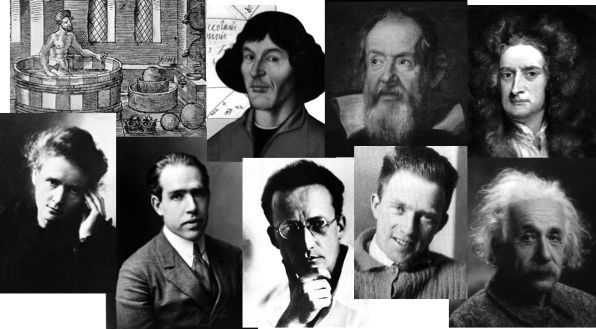
\includegraphics[width=1\textwidth]{imagenes/imagenes01/T01IM01.png}
	\caption{Arquímedes, Copérnico, Galileo, Newton, Marie Curie, Bohr, Schrödinger, Heisenberg y Einstein. \scriptsize{(Imagen del prof. Augusto Beléndez Vázquez, Universidad de Alicante.)}}
	\end{figure}

\subsection{Ramas de la física} 
\begin{itemize}
	\item Mecánica Clásica 
	\item Mecánica cuántica
	\item Teoría cuántica de campos 
	\item Teoría de la relatividad 
	\begin{itemize}
	\item Relatividad especial  
	\item Relatividad general 
     \end{itemize}
\item Mecánica Estadística 
\item Termodinámica
\item Mecánica de medios continuos 
\begin{itemize}
	\item Mecánica del sólido rígido, Mecánica de sólidos deformables, Elasticidad, Plasticidad.
	\item Mecánica de fluidos. 
\end{itemize}
Electromagnetismo 
\begin{itemize}
	\item Electricidad 
	\item Magnetismo 
\end{itemize}
\item Electrónica 
\item Astrofísica 
	\begin{itemize} \item Cosmología \end{itemize}
\item Geofísica (rama de la geología) 
\item Biofísica (rama de la biología) 
\item Óptica \footnote{Fuente: Wikipedia}
\end{itemize}


\subsection{La física según los físicos}


\begin{changemargin}{1cm}{1cm}

\textit{``La física es una ciencia cuyo objetivo es estudiar los componentes de la materia y sus interacciones mutuas. En función de estas interacciones la Física explica las propiedades de la materia en conjunto, así como los distintos fenómenos que observamos en la Naturaleza''.}  \small{(M. Alonso y E. J. Finn, ``Física. Vol. I: Mecánica'', Addison-Wesley Iberoamericana. México, 1986)}\normalsize{.} 


\vspace{2mm} \textit{``La historia de la física no puede entenderse como una mera yuxtaposición de descubrimientos y de observaciones experimentales a la cual se agregue su descripción matemática para dar lugar a teorías, sino que es también historia de los conceptos''}. \small{(Werner Heisenberg)}\normalsize{.} 


\textit{``La física se propone descubrir y dar forma matemática a las leyes universales que relacionan entre sí las magnitudes que intervienen en los fenómenos reales''.} \small{(Julio Palacios)}\normalsize{.} 

\textit{``La física es una creación del intelecto humano en su intento por comprender el mundo físico''. ``No es una mera colección de leyes, un catálogo de hechos sin relación mutua, sino que es una creación de la mente humana, con sus ideas y conceptos libremente inventados. Las teorías físicas tratan de dar una imagen de la realidad y de establecer su conexión con el amplio mundo de las impresiones sensoriales. La única justificación de nuestras estructuras mentales es si esa conexión se logra y de qué modo se hace'' }. \small{(Albert Einstein)}\normalsize{.} 

\textit{``Es equivocado pensar que la tarea de la física es averiguar cómo es la naturaleza. La física se refiere a lo que nosotros podemos decir de ella''}. (\small{Niels Bohr)}\normalsize{.} 

\textit{``La física es la ciencia de lo exótico, pero también es la ciencia de la vida cotidiana.''}  \small{(P. A. Tipler, ``Física para la ciencia y la tecnología'', Vol. 1 -Ed. Reverté. Barcelona, 1999)}\normalsize{.} 

\textit{``El cosmos también está dentro de nosotros: estamos hechos de materia estelar, y somos el medio para que el cosmos se conozca a sí mismo''.}\small{(Carl Sagan)}\normalsize{.}

\textit{``El milagro de la adecuación del lenguaje de las matemáticas para la formulación de las leyes físicas es un regalo maravilloso que ni entendemos ni merecemos''.}\small{(Eugene Wigner)}\normalsize{.}

\textit{``La ciencia es física. Todo lo demás es filatelia''.}\small{(Ernest Rutherford)}\normalsize{.}

\textit{``La ciencia será siempre una búsqueda, jamás un descubrimiento real. Es un viaje, nunca una llegada''.}\small{(Karl Popper)}\normalsize{.}

\textbf{\textit{``La física es lo ocupa a los físicos hasta avanzadas horas de la madrugada''.}} \small{(Richard Feynman)}\normalsize{.} Tal vez, la mejor definición de física.

\end{changemargin}

\textit{``La Física es como el sexo''}, dijo en cierta ocasión Richard Feynman.  \textit{``Está claro que puede tener algunos resultados prácticos, pero no lo hacemos por eso.''} La célebre cita de Feynman es perfectamente aplicable a toda la investigación científica básica.	
	

En conclusión, la física es mejor definirla en función de lo que se ocupa. Así, física es la ciencia que se ocupa de estudiar la mecánica clásica, la teoría cinética de gases, la teoría de campos, $\cdots$

\section{Conocimiento científico vs conocimiento ordinario}


Es \emph{conocimiento científico} es el que  adquiere el ser humano mediante los instrumentos de la metodología científica. El \emph{conocimiento ordinario} es el que adquiere por la experiencia y el sentido común.

Entre ambos tipos de conocimiento hay una estrecha relación: \emph{lo que hoy es conocimiento científico, mañana puede ser conocimiento ordinario}. Un claro ejemplo lo tenemos en la visión heliocentrista frente a la geocentrista, lo que hoy es conocimiento ordinario --la tierra gira entorno al sol-- hace unos siglos era considerado conocimiento científico.

\vspace{2mm}\centerline{\colorbox{LightYellow}{Experiencia + sentido común $\to$ conocimiento ordinario.}}\justify

 El objetivo de ambos tipos de conocimiento es objetivizar el mundo y racionalizarlo. 

\colorbox{LightYellow}{Conocimiento científico:} empieza donde acaba el conocimiento ordinario y para adquirirlo se precisa hacer uso del \colorbox{LightYellow}{\textit{`método científico'.}}

\section{El método científico}

Un `sistema científico' es una porción de universo que va a ser objeto de nuestro estudio.

El método científico es la sistemática formal de investigación que permite al físico interpretar los distintos problemas o fenómenos que se dan en ese sistema científico.

Pero ese método no es algo rígido, no hay un sistema fijo de reglas que nos permitan interpretar de una manera unívoca los fenómenos de ese sistema científico. El método científico no es un sistema inmutable. Ahora es válido, pues no contamos con otro, pero pueden inventarse otras leyes que se puedan aplicar a ese sistema científico.

El método científico se basa en:

\vspace{-2mm}\begin{itemize}
\item Tenemos un determinado sistema científico.
\vspace{-2mm} \item En él se dan una serie de fenómenos.
\vspace{-2mm} \item Nuestro objeto será interpretar esos fenómenos.	
\end{itemize}


\emph{Pasos a seguir para estudiar los fenómenos de cualquier sistema científico:}

\begin{enumerate}[a) ]
	\vspace{-2mm}\item Se formula el fenómeno $A$ \emph{con precisión y específicamente}.
	\vspace{-2mm}\item Observación de los \emph{hechos significativos} del fenómeno (los que nos ayuda a afirmar o refutar una ley).
	\vspace{-2mm}\item Proposición de \emph{hipótesis}, para explicar esos hechos significativos.
	\vspace{-2mm}\item Si las proposiciones formuladas en b) son correctas ascienden a la categoría de \emph{ley particular científica} (particular al fenómeno $A$).
	
	Si es correcta esta ley científica, nos explicará los hechos significativos y nos esclarecerá otros que aún no habíamos observado.
\end{enumerate}


Luego se repite esta operación con los fenómenos $B$, $C$, etc.

Finalmente, por \emph{inducción} de los fenómenos $A$, $B$, $C$, $\cdots$, es posible que se obtenga una \emph{ley general}. Si es válida, podremos llegar a descubrir nuevos fenómenos en nuestro sistema físico.

La ciencia que más se aproxima a este método es la \emph{física}.

\begin{ejem}{Galileo. Fenómeno $A$: `Caída libre de graves'}

Hechos significativos:
\vspace{-2mm}\begin{itemize}
	\item Observa que no influye la masa.
	\vspace{-2mm}\item Observa que \emph{casi} no influye el rozamiento con el aire.
	\vspace{-2mm}\item Observa que sí influye el tiempo: hay variación de la velocidad. Empieza a a caer lentamente y la velocidad va aumentando con el tiempo (aceleración).
\end{itemize}

Hipótesis: La aceleración es constante (de aquí se deduce una ley científica).
\end{ejem}

\begin{ejem}{Keppler. Fenómeno B: ¿De qué forma orbitan los planetas al sol?}

Hechos significativos:
\begin{itemize}
\vspace{-2mm} \item $2^a$ ley de Keppler: ``Las áreas barridas por unidad de tiempo es una constante'' (la velocidad areolar -- de áreas -- es constante).	
\end{itemize}

Hipótesis: Las órbitas son elípticas (esta hipótesis está de acuerdo con los hechos significativos).

De aquí se deducen sus tres leyes:
\vspace{-2mm}\begin{itemize} 
\vspace{-2mm}\item [-] Vueltas elípticas.
\vspace{-2mm}\item [-] Velocidad areolar constante.
\vspace{-2mm}\item [-] Los cuadrados de los tiempos de revolución coinciden con los cubos de los semi-ejes mayores de las elipses.
\end{itemize}	
\end{ejem}

\begin{ejem}{Newton: Ley de Gravitación Universal}

Intuye la ley de inercia a partir de la ley de caída de graves.

Con sus leyes construye el edificio de la mecánica clásica.	

Aplica a las observaciones de Keppler la mecánica y así obtiene la ``ley de gravitación universal''. Se trata de una `ley general', obtenida por inducción de las leyes de Galileo (Fenómeno $A$) y Keppler (fenómeno $B$). Explica estas leyes y las critica, ve sus fallos:

\begin{itemize}
\item [---] A Galileo: la aceleración no es constante, solo es aproximadamente constante.
\item [---] A Keppler: 
	\begin{itemize}
	\item [-] La órbitas no son totalmente elípticas. 	
	\item [-] La velocidad areolar es aproximadamente constante.
	\item [-] Los tiempos de revolución al cuadrado son aproximadamente igual a los cubos de los semiejes mayores.
	\end{itemize}
\end{itemize}
\end{ejem}

\begin{multicols}{2}
Más tarde se observa que Mercurio no describe una elipse, su eje se desvía, describe una `roseta'.

La segunda ley de Newton ya no es válida.

Aparece una ley mejor que la anterior: ``Teoría de la Relatividad General'', de Albert Einstein.
\begin{figure}[H]
	\centering
	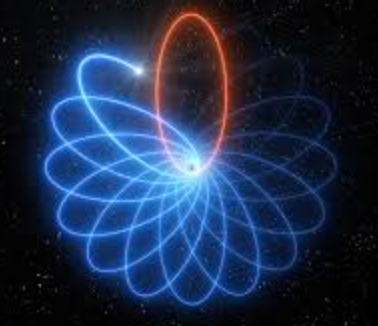
\includegraphics[width=.4\textwidth]{imagenes/imagenes01/T01IM02.png}
	\end{figure}
\end{multicols}

\begin{multicols}{2}
$\quad$

Los rayos de luz se comportan como si tuviesen `masa': cuando un rayo de luz pasa por el lado de un cuerpo pesado siente la acción de la gravedad de éste y el haz se curva.

\begin{figure}[H]
	\centering
	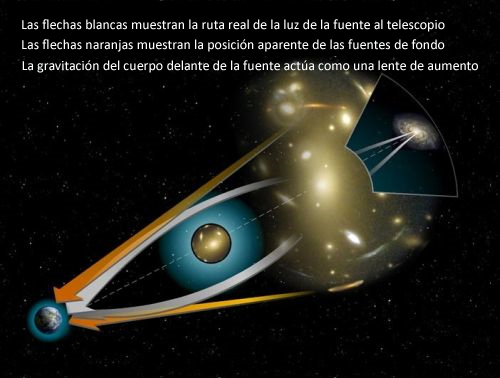
\includegraphics[width=.4\textwidth]{imagenes/imagenes01/T01IM03.png}
	\end{figure}
\end{multicols}	
	

\section{Modelo matemático de un sistema físico}
	
En un sistema físico, por ejemplo el conjunto `Tierra-Sol' hay multitud de fenómenos que observar. Centrémonos en el estudio del periodo de revolución de la Tierra alrededor del Sol. Ahora es cuando aparece el \emph{modelo matemático} del sistema físico.

\begin{figure}[H]
	\centering
	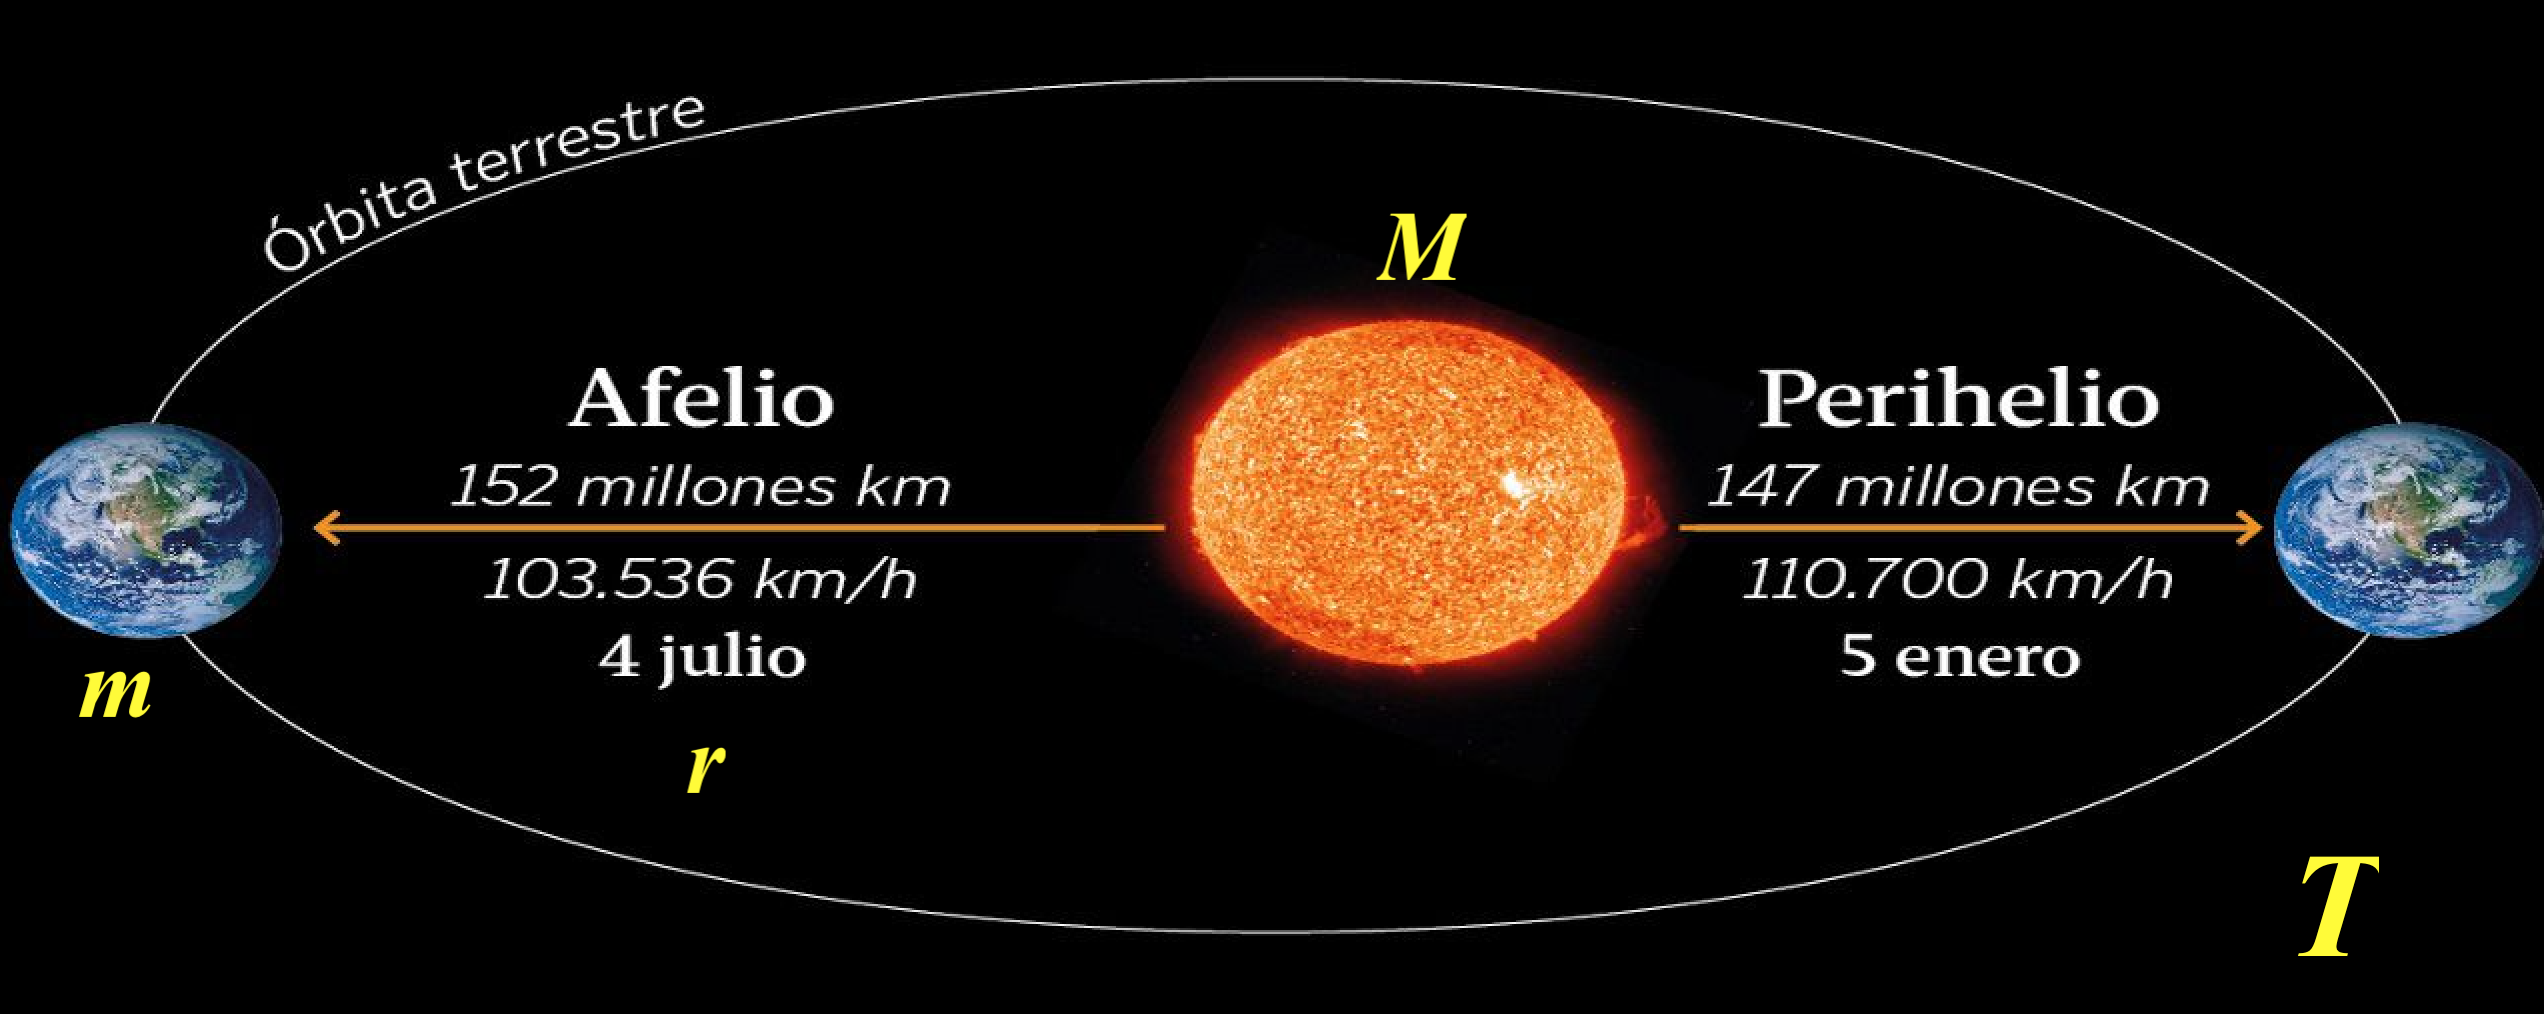
\includegraphics[width=.9\textwidth]{imagenes/imagenes01/T01IM04.png}
	\end{figure}
	
Aplicando las leyes de la mecánica a este modelo matemático encontraremos el periodo de revolución, $T$. Si el modelo es bueno, está de acuerdo con la experiencia, usaremos esta fórmula para, por ejemplo, la rotación del electrón alrededor del núcleo de Hidrógeno.

\vspace{10mm} %****************************
¿Cuántos modelos matemáticos puede tener un sistema físico? Respuesta: ``Un sistema físico puede tener tantos modelos matemáticos como fenómenos haya que estudiar en él''.
	
\newpage %**********************************************
\begin{myblock}{Feynman y la física.}
\begin{small}	
Entre 1961 y 1963, el famoso científico Richard Feynman dio una serie de conferencias de física en Caltech. Las notas de esas clases fueron luego compiladas y presentadas como \textbf{The Feynman Lectures}, y son considerados los libros de física más exitosos de la historia, con más de 1.5 millones de copias vendidas. 
 
\vspace{2mm} ``Uno podría preguntar, porqué es que no podemos enseñar física mostrando primero las leyes básicas y luego demostrando cómo funcionan en todas las circunstancias posibles, de la misma forma en que lo hacemos con la geometría euclidiana, donde enunciamos los axiomas y luego hacemos todo tipo de deducciones. No lo podemos hacer de esta manera por dos razones: en primera, porque aún no conocemos todas las leyes básicas, de hecho existe una ‘frontera creciente’ de ignorancia. Y en segunda, la correcta enunciación de las leyes físicas involucra ideas poco familiares que requieren de matemáticas avanzadas para su descripción. Por lo tanto, requerimos de una cantidad considerable de preparación tan sólo para saber lo que significan las palabras que estamos usando en estas leyes. Siendo así, no podemos enunciarlas en general, sino sólo de parte en parte.
Ahora bien, cada parte del total de la naturaleza es una aproximación a la verdad completa, o bien la verdad completa tal y como la podemos concebir. De hecho, todo lo que sabemos no es más que un tipo de aproximación, porque sabemos que no conocemos todas las leyes. Por lo tanto, las cosas que aprendemos deben ser desaprendidas más tarde, o por lo menos corregidas.''

\vspace{2mm} ``El principio de la ciencia, o más bien casi su definición, es ésta: La prueba de todo conocimiento es el experimento. El experimento es el único juez de una verdad científica.''

\vspace{2mm} ``Finalmente, y lo más interesante, es que filosóficamente estamos diciendo que esta ley de aproximación hace que siempre estemos equivocados: aún un efecto muy pequeño en nuestro conocimiento puede tener implicaciones muy profundas en nuestras ideas acerca del mundo.''
\end{small}
\hspace{20mm} \rightline{\textit{\normalsize{Por Alfonso Araujo, el 6 agosto, 2019. }}NAUKAS.}
\end{myblock}


\part{I Mecánica clásica}


\begin{myalertblock}{Mecánica cásica}

La Mecánica es la parte de la física que tiene por objeto el estudio de los movimientos de los cuerpos materiales.

Sus partes principales son

\begin{itemize}
\item \emph{Cinemática}: Parte de la Mecánica que estudia el movimiento de los cuerpos materiales sin atender al por qué lo hacen.
\item \emph{Dinámica}: Parte de la Mecánica	 que estudia bajo qué condiciones se mueven los cuerpos materiales.
\item \emph{Estática}:  Parte de la Mecánica que estudia las condiciones de equilibrio de los cuerpos materiales (respecto de un determinado observador).
\end{itemize}

\end{myalertblock}
 
\chapter{Cinemática de la partícula}


\setlength{\parindent}{0cm}


\section{Sistema de referencia}

\begin{multicols}{2}
Supongamos dos observadores distintos, uno situado en la Tierra y el otro en el Sol, observando el movimiento de la Luna.

Ambos describen el movimiento de la Luna de dos modos completamente distintos. ¿Cuál de los dos tienen razón?

Ambos, evidentemente, la descripción del movimiento depende de donde de observe éste. Es necesario un \colorbox{LightYellow}{\emph{Sistema de Referencia}}, es decir,  \colorbox{LightYellow}{un origen} (un punto),  \colorbox{LightYellow}{unos ejes} (base de vectores ortonormal)  \colorbox{LightYellow}{y un reloj} (origen de tiempos) sobre el cual referir el movimiento del cuerpo observado.
\begin{figure}[H]
		\centering
		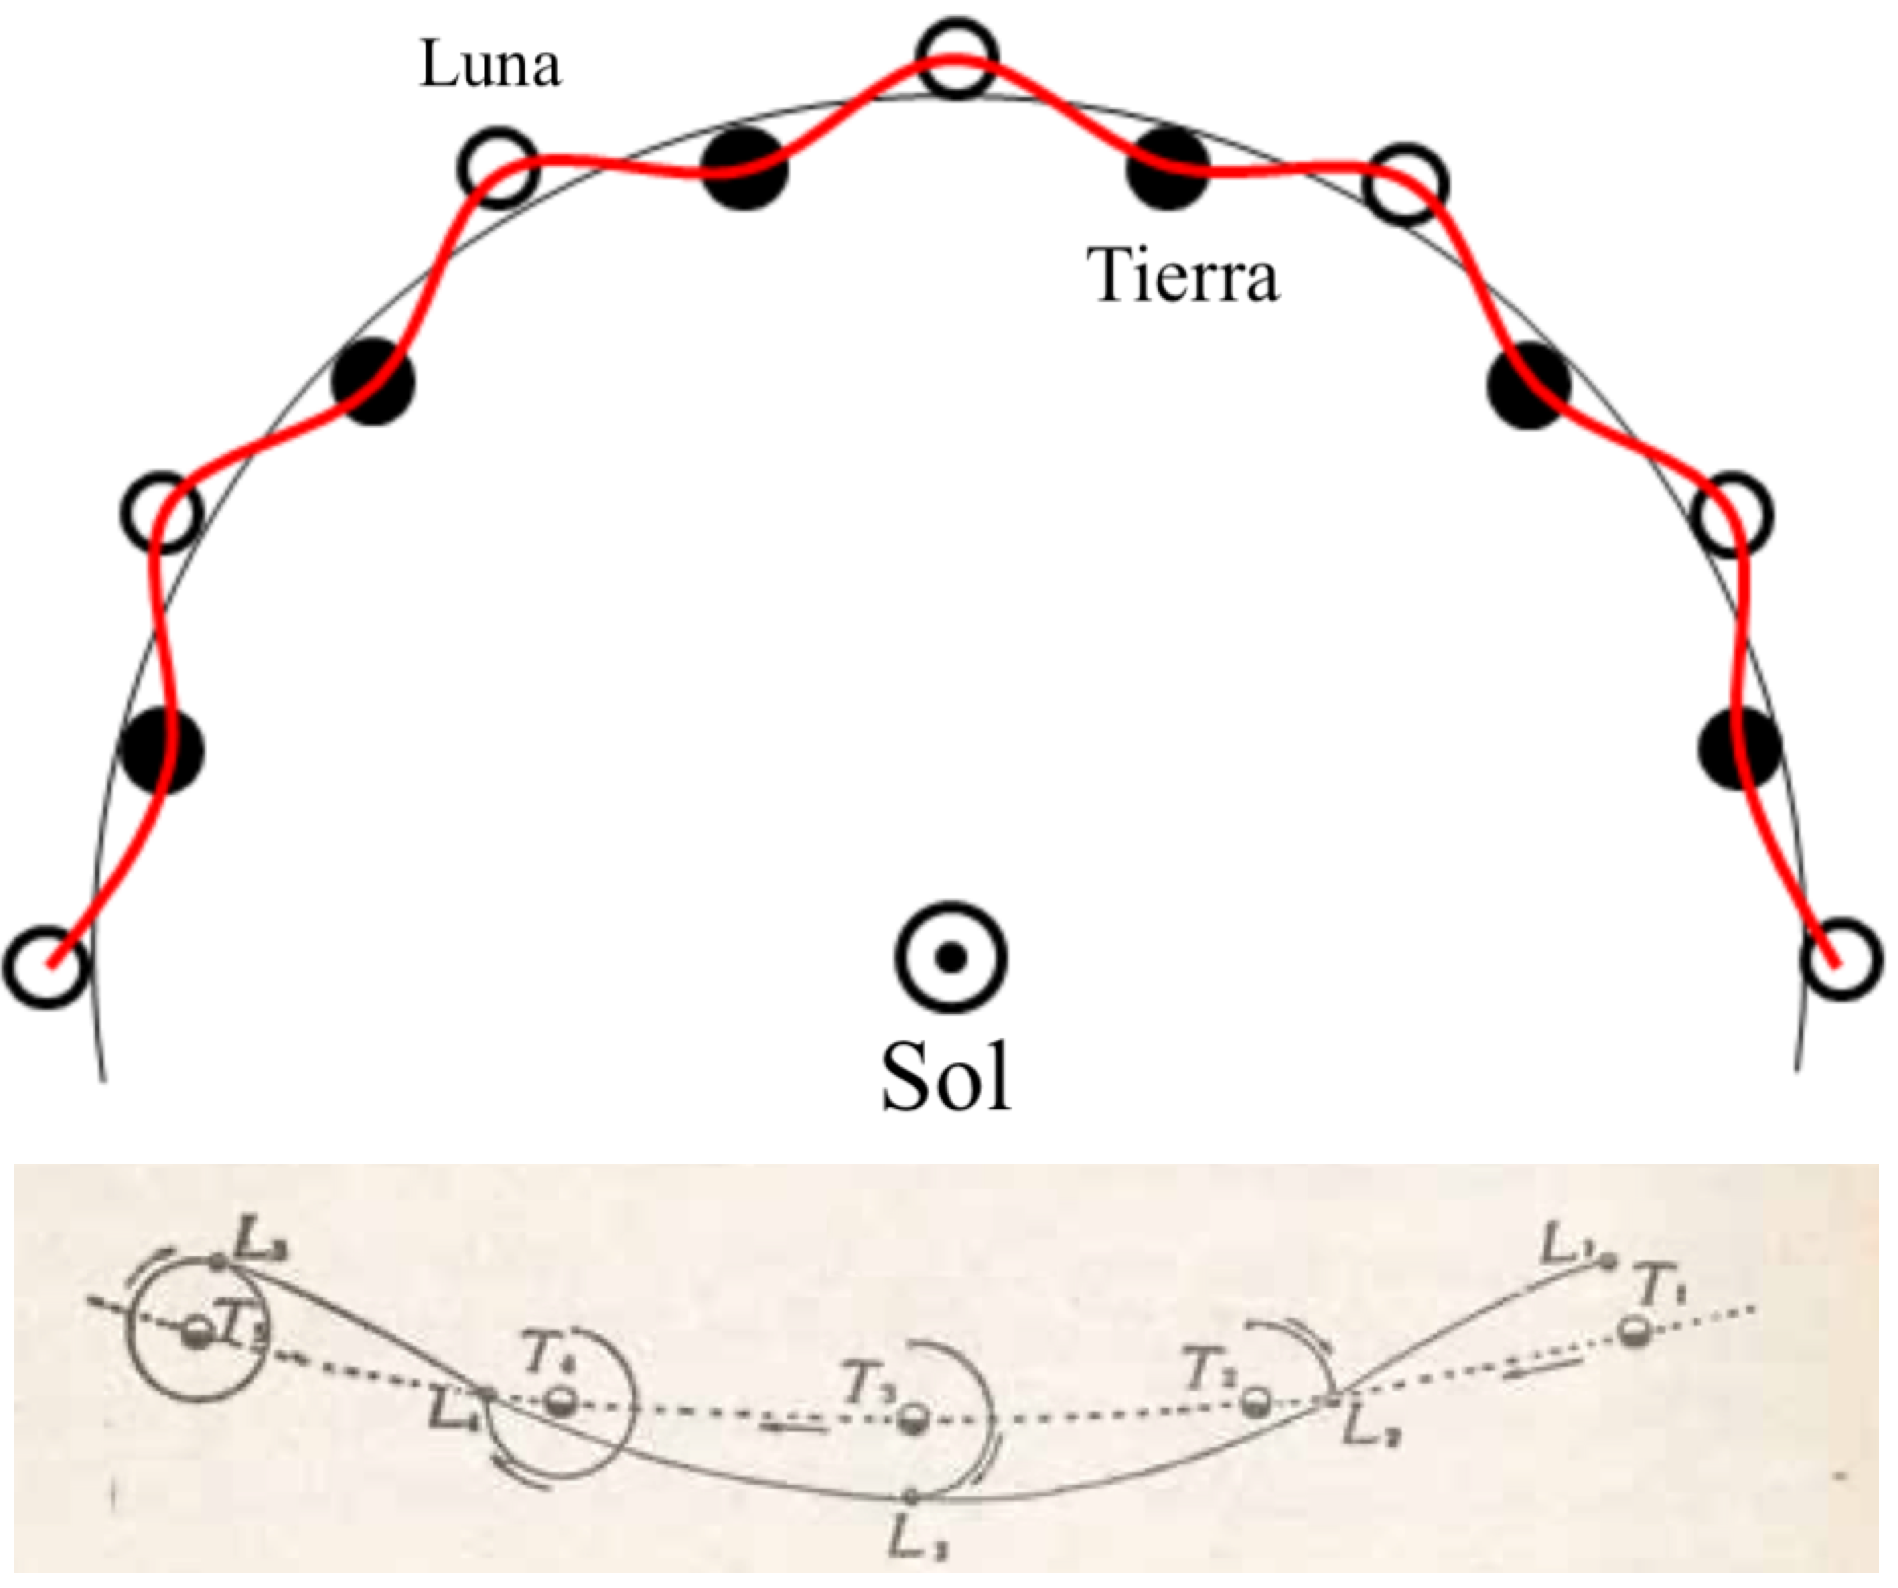
\includegraphics[width=.5\textwidth]{imagenes/imagenes02/T02IM01.png}
	\end{figure}
\end{multicols}

Un sistema de referencia es un conjunto de convenciones usado por un observador para poder medir la posición y otras magnitudes de un sistema físico. Las trayectorias medidas y el valor numérico de muchas magnitudes son relativas al sistema de referencia que se considere, por esa razón, se dice que el movimiento es relativo.

\begin{multicols}{2}
En mecánica clásica un sistema de referencia consta de un punto espacial fijo llamado origen $\mathcal O$, una base de vectores ortonormal orientada $\vec i,\; \vec j,\; \vec k$ \footnote{En el Apéndice \ref{Vectores} se recuerda el concepto de `Base OrtoNormal'.}  y un reloj para el origen de tiempos (dados dos sistemas de coordenadas de ese tipo, existe un giro y una traslación que relacionan las medidas de esos dos sistemas de coordenadas).
\begin{figure}[H]
		\centering
		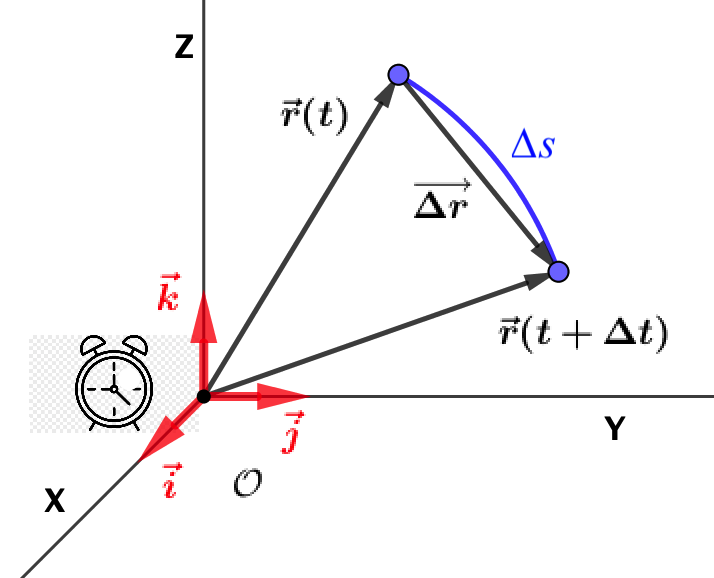
\includegraphics[width=.5\textwidth]{imagenes/imagenes02/T02IM02.png}
	\end{figure}
\end{multicols}

Cuando $\Delta t \to 0$, $\Delta \vec r$ es tangente a la trayectoria y $\abs{\Delta \vec r} \approx \Delta s$.

Por definición, la velocidad es:

\begin{equation}
\label{velocidad}
\subrayado{
 \vec v= \lim_{\Delta t\rightarrow 0 } \dfrac {\Delta \vec r}{\Delta t}	= \dv{\vec r}{t}
 }
\end{equation}


$\displaystyle \vec v= \lim_{\Delta t\rightarrow 0} \dfrac{\Delta \vec r}{\Delta s}\cdot \dfrac {\Delta s}{\Delta t} =\lim_{\Delta s\rightarrow 0} \dfrac{\Delta \vec r}{\Delta s}\cdot \lim_{\Delta t\rightarrow 0} \dfrac {\Delta s}{\Delta t}= \vec u_T \cdot v$

$\displaystyle \vec u_T=\lim_{t\rightarrow 0} \dfrac{\Delta \vec r}{\Delta s}$: dirección de la recta tangente a la trayectoria y módulo unidad.

$\displaystyle v=\lim_{t\rightarrow 0} \dfrac {\Delta s}{\Delta t}$: un escalar (número real).

\begin{equation}
\vec v=v\cdot \vec u_T
\end{equation}

El \colorbox{LightYellow}{vector velocidad} es, en todo momento, \colorbox{LightYellow}{tangente a la trayectoria} siendo $v$ su módulo (celeridad)\footnote{Celeridad = módulo del vector velocidad.}:
$\quad v=\abs{\vec v}=\sqrt{v_x^2+v_y^2+v_z^2}$

En el SI \emph{(Sistema Internacional de Unidades)}, la velocidad se mide en $\mathrm{m/s} = \mathrm{m\cdot s}^{-1}$

\section{Componentes cartesianas del vector velocidad}
Puesto que el vector de posición de la partícula que se mueve, $\vec r$, se puede expresar en coordenadas cartesianas en nuestro sistema de referencia como: $\;\;\vec r=x\cdot \vec i+y\cdot \vec j+z\cdot \vec k$, para el vector velocidad tendremos:

$\displaystyle \boldsymbol{\vec v}=\dv{\vec r}{t}= \dv{x}{t}\cdot \vec i+\dv{y}{t} \cdot \vec j+\dv{z}{t} \cdot \vec k  \boldsymbol{=v_x\cdot \vec i+v_y\cdot \vec j+v_z\cdot \vec k}$


\section{Movimiento de una partícula en un plano. Componentes polares de la velocidad} \label{velocidad-polares}

\begin{multicols}{2}
$\displaystyle \vec v= \dv{t} \vec 
r = \dv{t} (r\cdot \vec u_r)= $

$\displaystyle=\dv{r}{t} \cdot \vec u_r + r \cdot \dv{\vec u_r}{t}$

$\displaystyle  \dv{\vec u_r}{t}  \; \parallel \;\vec u_\theta$

Con $\quad \vec u_\theta \; \bot \; \vec u_r \quad (*)$ 
\begin{figure}[H]
		\centering
		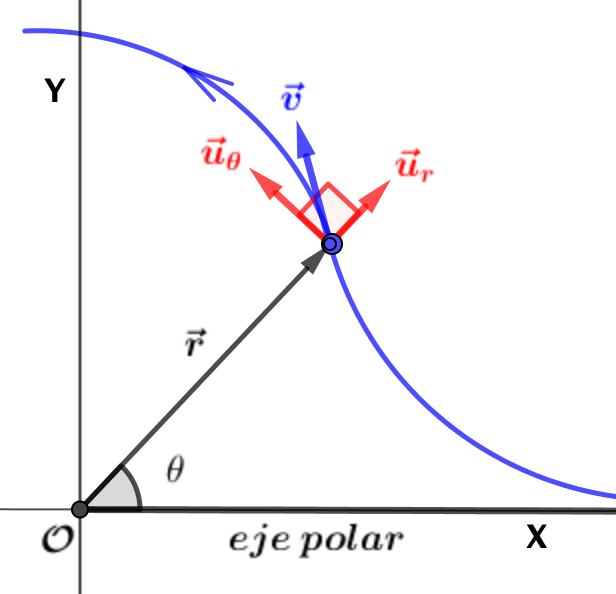
\includegraphics[width=.3\textwidth]{imagenes/imagenes02/T02IM03.png}
		\end{figure}
\end{multicols}

\begin{footnotesize}
\textcolor{gris}{$\displaystyle (*) \quad \dv{t} (\vec u_r \cdot \vec u_r)=\dv{t} 1=0$}

\textcolor{gris}{Por otra parte: $\displaystyle \dv{t} (\vec u_r \cdot \vec u_r)=\dv{\vec u_r}{t}\cdot \vec u_r+\vec u_r \cdot \dv{\vec u_r}{t}=2\vec u_r \dv{\vec u_r}{t}$}

\textcolor{gris}{Luego $\displaystyle \vec u_r \dv{\vec u_r}{t}=0 \Rightarrow \vec u_r \;\bot\; \dv{\vec u_r}{t}\;\ \parallel ;\vec u_\theta \qquad \Box$}

\textcolor{gris}{Hemos usado que $\vec u \cdot \vec v=\abs{\vec u} \;\abs{\vec v}\; \cos (\varphi_{\vec u, \vec v})$, por lo que $\vec u \cdot \vec v=0 \leftrightarrow \vec u \bot \vec v$ y que $\abs{\vec u_r}=\abs{\vec u_\theta}=1$. También que $\vec r=r\; \vec u_r$}
\end{footnotesize}

Transportando estos vectores al origen: \textcolor{gris}{$\alpha=90^o-\theta$}
\begin{multicols}{2}
$\begin{cases} \;\;\vec u_r=\;\;\cos \theta\; \vec i + \sin \theta\; \vec j \\ \\ \;\;\vec u_\theta = -\sin \theta \; \vec i + \cos \theta \;\vec j \end{cases}$
\begin{figure}[H]
		\centering
		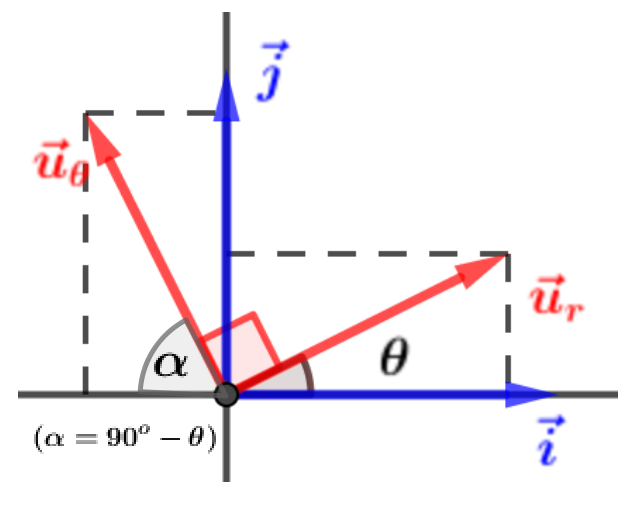
\includegraphics[width=.25\textwidth]{imagenes/imagenes02/T02IM04.png}
		\end{figure}
\end{multicols}

Derivando: $\quad \displaystyle \dv{\vec u_r}{t}=\dv{t} (\cos \theta\; \vec i + \sin \theta\; \vec j)=-\sin \theta \dv{\theta}{t} \; \vec i + \sin \theta \dv{\theta}{t} \; \vec j=(-sin \theta \;\vec i+ \cos \theta \; \vec j)\; \dv{\theta}{t} \quad \Rightarrow \qquad 	\boldsymbol{\dv{\vec u_r}{t}=\vec u_\theta \cdot \dv{\theta}{t}}\quad$ que es la relación matemática que buscábamos.

\begin{equation}
\label{veloc-polares}
\subrayado{
\vec v=\vec u_r \cdot \dv{r}{t} + \vec u_\theta \cdot r\cdot \dv{\theta}{t} 
}
\end{equation}

El primer de término es la `velocidad radial' y el segundo la `velocidad transversal'. Conclusión: \emph{La velocidad radial es perpendicular a la velocidad transversal}.

\section{Movimiento rectilíneo}

Movimiento rectilíneo es el que se realiza a lo largo de una línea recta. Llamamos eje $OX$ a la recta que describe esta trayectoria y fijamos un punto $\mathcal O$ como origen. La posición del objeto al cabo de de un tiempo $T$ viene dada por el escalar, en este caso, $r(t)$ que mide la distancia del móvil al origen $\mathcal O$. En estas condiciones:

$\displaystyle \vec v= \dv{\vec r}{t} \to \int_{r_0}^{r} \dd r=\int_{t_0}^{t}v\; \dd t \quad \Rightarrow \qquad  \quad r-r_0=\int_{t_0}^{t}v\; \dd t $

En el caso particular de que $ \; v=cte	\;$, independiente del tiempo, la expresión anterior queda como: $ \;\; r-r_0=v\; ( t-t_0 ) $

Consideremos ahora que el observador no está situado sobre la recta de la trayectoria o eje de movimiento:


\begin{multicols}{2}
$\displaystyle \vec v=\dv {\vec r}{t}\to \int_{\vec r_0}^{\vec r} \dd r = \int_{t_0}^{t} \vec v \ \dd t$ 

de donde: $\vec r-\vec r_0=\displaystyle \int_{t_0}^{t} \vec v \ \dd t$

\begin{figure}[H]
		\centering
		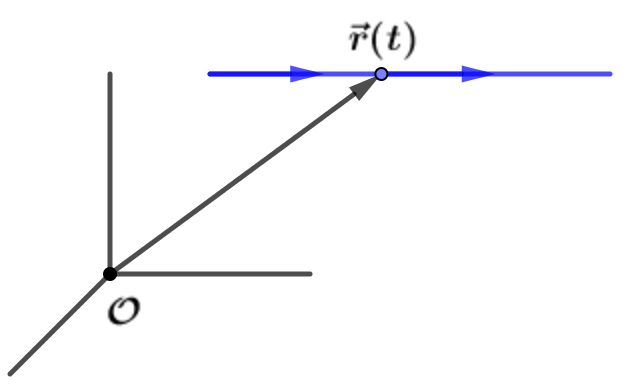
\includegraphics[width=.25\textwidth]{imagenes/imagenes02/T02IM05.png}
		\end{figure}
\end{multicols}
En el caso particular de que $\boldsymbol{ \;\vec v= \overrightarrow{cte}\; }$, se tiene:

\begin{equation}
\label{MRU}
	 \vec r-\vec r_0=\vec v\; (t-t_0) 
\end{equation}

que es la ecuación del \textbf{MRU} (movimiento rectilíneo uniforme, $\vec v = \overrightarrow{cte}$) en tres dimensiones.

\vspace{-4mm}\section{Movimiento circular. Velocidad angular.}

Llamamos movimiento circular a aquel que describe una circunferencia, por tanto, tiene lugar en un plano. Usaremos coordenadas polares que son más útiles en este caso.

Al ser la trayectoria una circunferencia, $R=\abs{\vec R}=cte$, por lo que:

\begin{multicols}{2}

$\displaystyle \vec v=\dv{\vec R}{t}=\dv{(R\;\vec u_R)}{t}=$

$\displaystyle =\cancelto{0}{\dv{R}{t}}\;\vec u_R+R\; \dv{\vec u_R}{t}$
\begin{figure}[H]
		\centering
		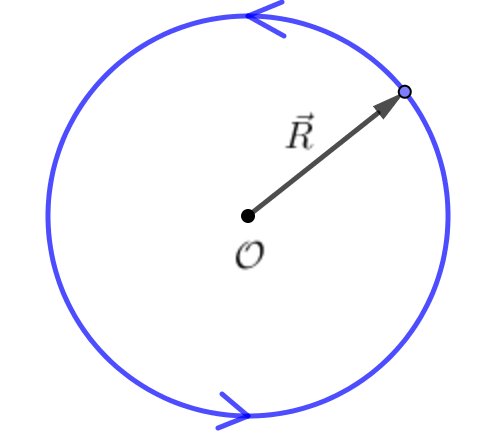
\includegraphics[width=.2\textwidth]{imagenes/imagenes02/T02IM06.png}
		\end{figure}
\end{multicols}

Recordando la ecuación \ref{veloc-polares}:
$\qquad \displaystyle \vec v=R\cdot \dv{\theta}{t}\;\vec u_\theta=R\cdot \omega \; \vec u_\theta$,

Siendo $\displaystyle \omega=\dv{\theta}{t}$ el módulo de la velocidad angular (ángulo barrido en la unidad de tiempo), que en el $SI\;$\footnote{ SI= Sistema Internacional de unidades.} se mide en $\mathrm{s}^{-1}$. Es usual expresarla en $\text{rad}\cdot \mathrm{s}^{-1}$ o $\text{rpm}$.\footnote{ rpm=revoluciones por minuto.}

Supongamos ahora que el observador no se encuentra situado en el centro de la circunferencia que describe la partícula que se mueve sino en una recta perpendicular a ella que pasa por su centro.

\begin{multicols}{2}
Respecto de $\mathcal O'$

$\displaystyle \vec v = \textcolor{gris}{\vec v_{\mathcal O'}}=\dv{\overrightarrow{ r }}{t} = \dv{t}(\overrightarrow{\mathcal O \mathcal O'}+\vec R )=$

$\displaystyle =\dv {\vec R} {t}=R\cdot \omega\; \vec u_\theta\; ; \qquad \textcolor{gris}{\overrightarrow{\mathcal O \mathcal O'}=\overrightarrow{cte}}$

\begin{figure}[H]
		\centering
		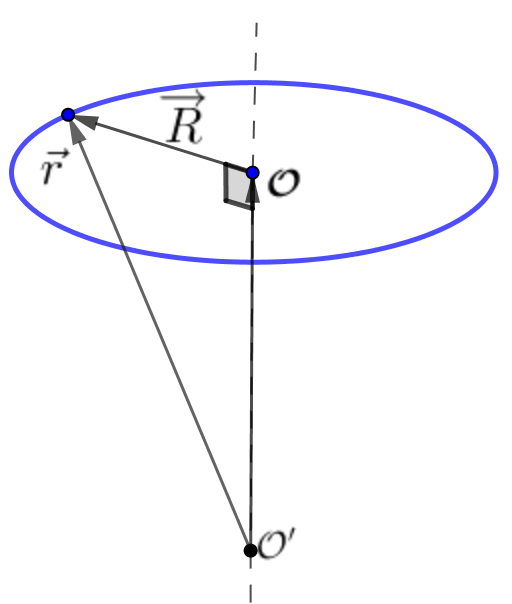
\includegraphics[width=.25\textwidth]{imagenes/imagenes02/T02IM07.png}
		\end{figure}
\end{multicols}

\begin{multicols}{2}
Sea $\mathcal O'$ un punto cualquiera de la recta perpendicular a la trayectoria que pasa por el centro, $(\mathcal O)$, de la figura:
$\quad R=r\cdot \sin \alpha$

Luego $\quad \vec v= \omega \cdot r \cdot \sin \alpha \;\; \vec u_\theta$

Recordando la definición de `producto vectorial' de dos vectores (y la regla del sacacorchos para determinar su sentido),

\begin{figure}[H]
		\centering
		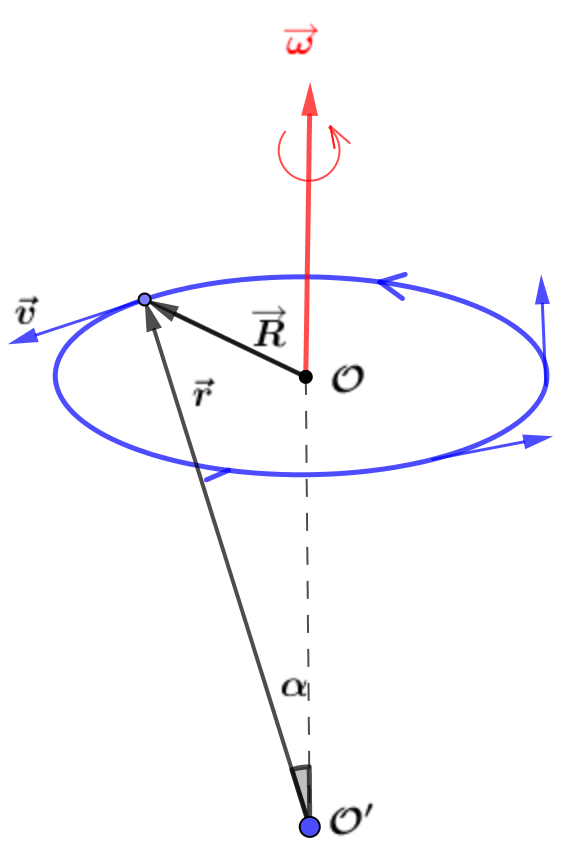
\includegraphics[width=.3\textwidth]{imagenes/imagenes02/T02IM08.png}
		\end{figure}
\end{multicols}

\begin{equation}
\label{v-angular}
\subrayado{
\vec v=\vec \omega \times \vec r
}
\end{equation}
donde $\vec \omega$ es el vector velocidad angular.

El vector velocidad angular es perpendicular al plano del movimiento en es sentido de avance de un sacacorchos que gira en el mismo sentido en que lo hace la partícula, en módulo se tiene que $ v=\omega\; r\; \sin \alpha$. 

\begin{multicols}{2}
$\quad$

\emph{Nótese que esto solo es válido para movimientos circulares con el observador situado perpendicularmente al centro de la trayectoria, es decir, siempre que $R=cte \; \wedge \; alpha=cte$.}  
\begin{figure}[H]
		\centering
		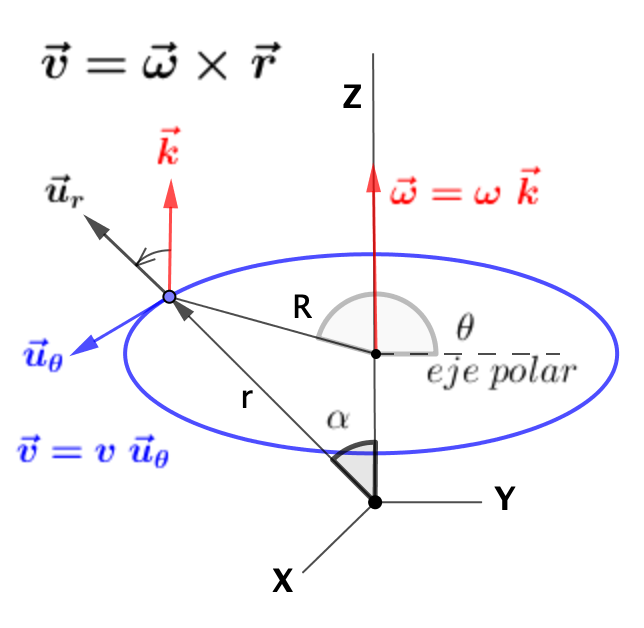
\includegraphics[width=.4\textwidth]{imagenes/imagenes02/T02IM09.png}
		\end{figure}
\end{multicols}

Como $\displaystyle \omega=\dv{\theta}{t}\to  \int_{\theta_0}^{\theta}\dd \theta = \int_{t_0}^t \omega \;\dd t \Rightarrow \;\; \;\theta-\theta_0=\int_{t_0}^t \omega \;\dd t\;$

En el caso particular en que $\; \theta = cte$, tendremos: $\;\theta-\theta_0= \omega \;(t-t_0)\;$

Un movimiento es \textbf{periódico} si al pasar un determinado tiempo $\boldsymbol{T}$ llamado \textit{\textbf{periodo}},  todas las variables que describen el movimiento vuelven a tomar el mismo valor. \textit{El movimiento circular uniforme, en que $\omega=cte$, es periódico.}

\textbf{Relación entre $\boldsymbol{T}$ y $\boldsymbol{\omega}$}


\begin{multicols}{2}
Empezamos a contar el tiempo (\emph{origen de tiempos}) cuando la partícula está en el punto A en que el ángulo, medido desde el eje polar, es $\theta_0$. Las variables que describan el movimiento volverán a tomar el mismo valor al cabo de una vuelta:

\begin{figure}[H]
		\centering
		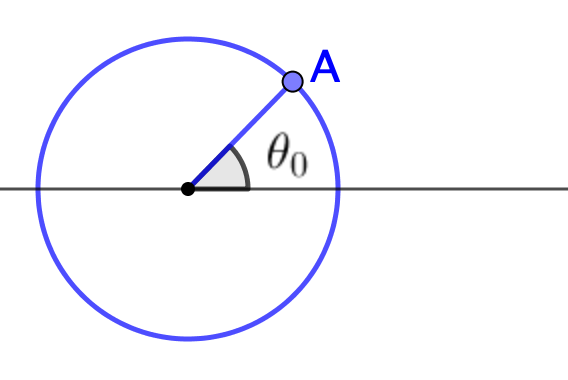
\includegraphics[width=.45\textwidth]{imagenes/imagenes02/T02IM10.png}
		\end{figure}
\end{multicols}

$\theta=\theta_0+\omega \; T \to $, al cabo de una vuelta $\theta=\cancel{\theta_0}+2\pi=\cancel{\theta_0}+\omega \; T \to 2\pi=\omega \; T$

de donde:

\begin{equation}
\label{periodo-vel-angular}
T = \dfrac {2\pi}{\omega} \qquad \vee \qquad \subrayado{\omega=\dfrac{2\pi}{T}}	
\end{equation}

$T$ en $s$. Se llama \textbf{\emph{frecuencia, $\nu$}} a la inversa del periodo y se expresa en $s^{-1}\;(=Hz=rps)$\footnote{rps: revoluciones por segundo}.

\begin{equation}
T=\dfrac 1 \nu	 \qquad \qquad \omega=2\pi\; \nu
\end{equation}

La velocidad angular se usa para movimientos angulares (para movimientos aproximadamente circulares se usa la velocidad angular media).

\section{Aceleración}

La \emph{aceleración} es una magnitud vectorial íntimamente ligada con la \emph{fuerza}. Por definición, la aceleración es: 

\begin{multicols}{2}

\begin{figure}[H]
		\centering
		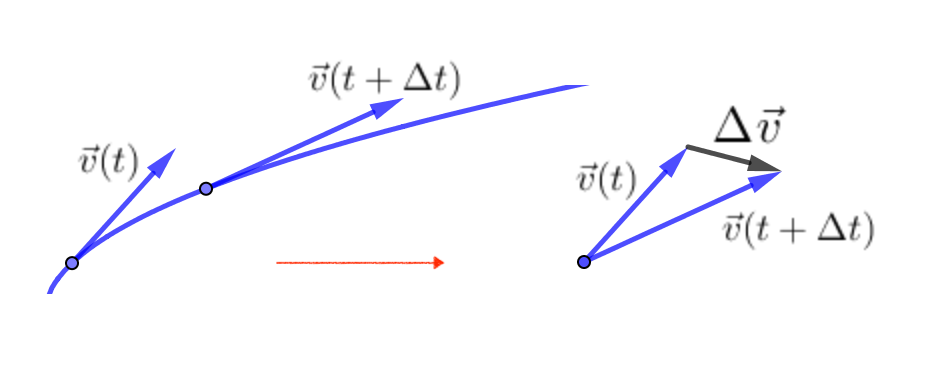
\includegraphics[width=.6\textwidth]{imagenes/imagenes02/T02IM11.png}
		\end{figure}
\vspace{3mm}
\begin{equation}
\label{aceleracion}
\subrayado{
\vec a= \lim_{\Delta t\rightarrow 0 } \dfrac{\Delta \vec v}{\Delta t}=\dv{\vec v}{t}	
}
\end{equation}
\end{multicols}

\begin{multicols}{2}
Características de $\vec a$:

$\quad$

Mira siempre hacia el interior de la concavidad de la trayectoria.
\begin{figure}[H]
		\centering
		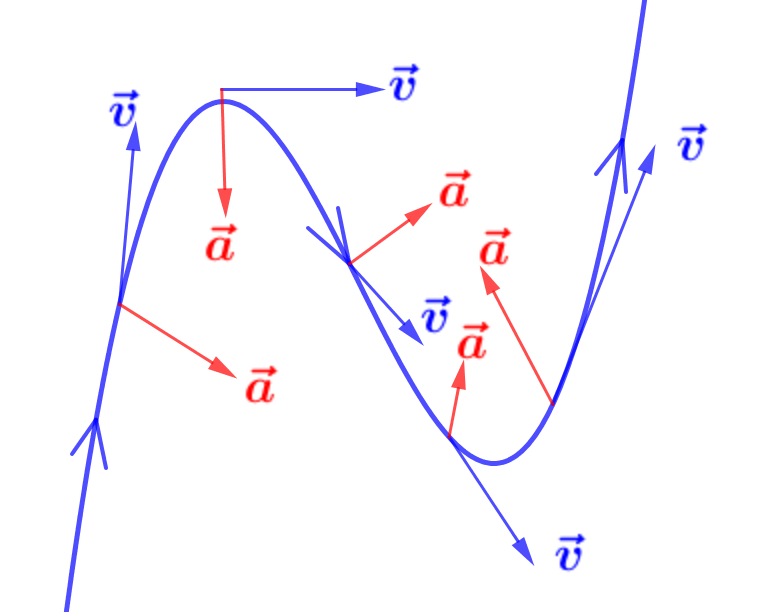
\includegraphics[width=.3\textwidth]{imagenes/imagenes02/T02IM12.png}
		\end{figure}
\end{multicols}

\begin{figure}[H]
		\centering
		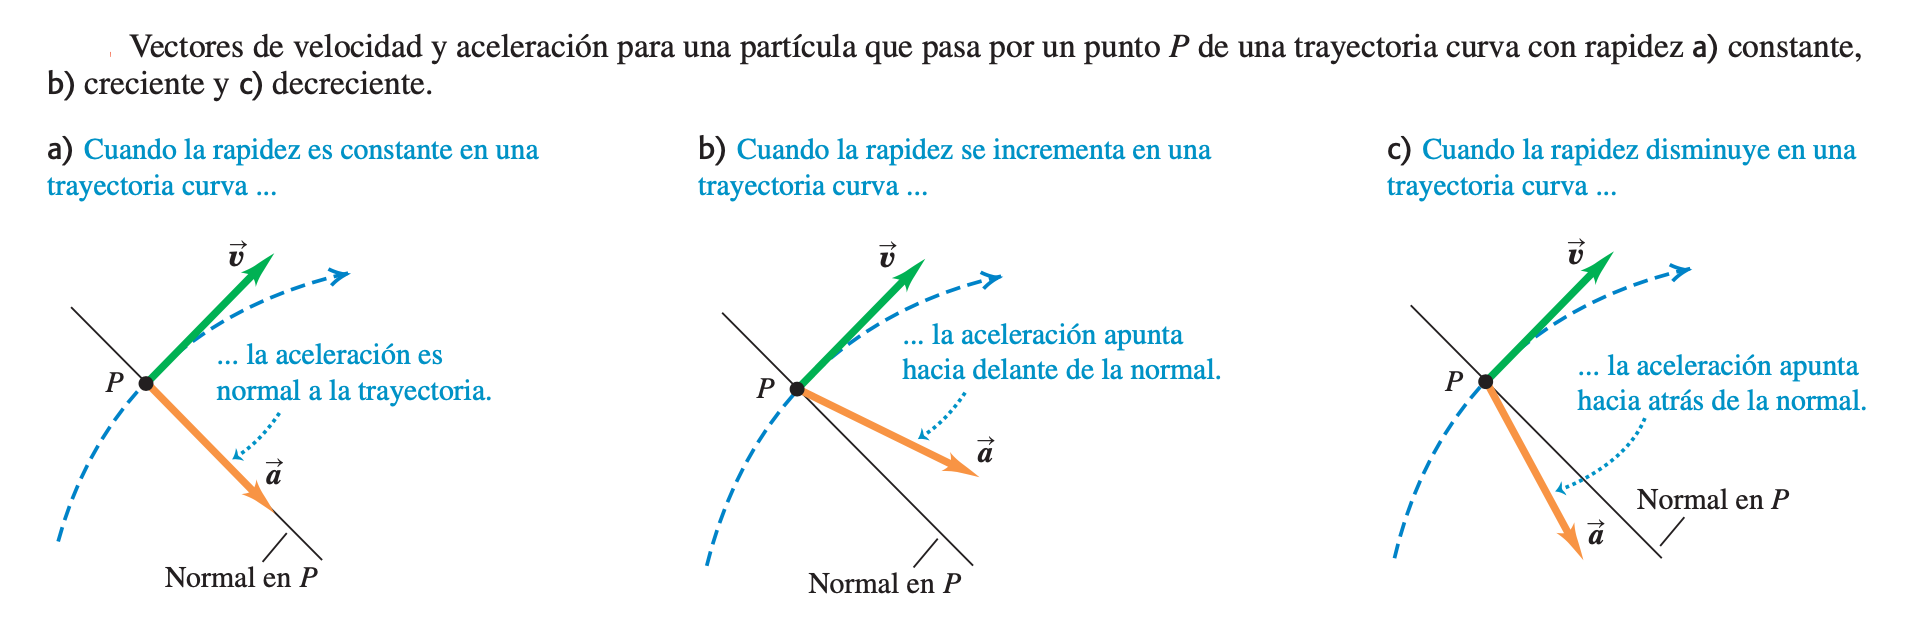
\includegraphics[width=1\textwidth]{imagenes/imagenes02/T02IM15.png}
		\end{figure}

Resolvamos el problema de determinar $\vec v$ y $\vec r$ conocido el vector $\vec a$ y las condiciones iniciales $\vec v_0$ y $\vec r_0$:

De la definición de aceleración, ecuación \ref{aceleracion}: $\;\;\dd \vec v= \vec a\; \dd t\;$ . Integrando entre $t_o$ y $t$, intervalo en que las velocidades son $\vec v_0$ y $\vec v$ respectivamente:

$\displaystyle \int_{\vec v_0}^{\vec v}\dd \vec v= \int_{t_0}^{t} \vec a\; \dd t \quad \to \qquad \vec v=\vec v_0+\int_{t_0}^{t} \vec a\; \dd t$

\subsection{Movimiento rectilíneo uniformemente acelerado}

Particularizemos para el caso en que $\boldsymbol{ \vec a=\overrightarrow{cte} }$, \textbf{MRUA} \emph{(Movimiento rectilíneo uniformemente acelerado --$\vec a=\overrightarrow{cte}$--):}

En estas condiciones, $\vec a=\overrightarrow{cte}$, se tiene que:

\begin{equation}
\label{MRUAv}
	\vec v=\vec v_0+\vec a\; (t-t_0)
\end{equation}

$\displaystyle \vec v=\dv{\vec r}{t} \to \dd \vec r=\vec v\dd t : \quad \int_{\vec r_0}^{\vec r}\dd \vec r=\int_{t_0}^t \vec v\;\dd t \to$, teniendo en cuenta \ref{MRUAv}:

$\displaystyle \vec r-\vec r_0=\int_{t_0}^t 
\qty(\; \vec v_0+\vec a\; (t-t_0) \;)
\; \dd t;\; \qquad \vec a=\overrightarrow{cte} \; \wedge \; \vec v_0=\overrightarrow{cte'} \Rightarrow\;:$

\begin{equation}
\label{MRUAr}
	\vec r=\vec r_0+ \vec v_0\; (t-t_0)+\dfrac 1 2 \vec a\; (t-t_0)^2
\end{equation}

Las ecuaciones del MURA en una dimensión (observador situado en la recta de la trayectoria) las ecuaciones son:
$$v=v_0+a\;(t-t_o) \qquad \wedge \qquad r=r_0+v_0\;(t-t_0)+\dfrac 1 2 \; a \; (t-t_0)^2$$

\emph{Cuando la aceleración es constante, la trayectoria es una parábola} ($r \propto t^2$).


\subsection{Componentes cartesianas de la aceleración}

$\displaystyle \vec a=\dv{\vec v}{t}=\textcolor{gris}{
\dv{t}\left( \dv{\vec r}{t}  \right)
}=\dv[2]{\vec r}{t}$

$\displaystyle 
\vec a=\dv{v_x}{t}\;\vec i+\dv{v_y}{t}\;\vec j+\dv{v_z}{t}\;\vec k
\qquad \qquad
\vec a= \dv[2]{x}{t}\;\vec i+\dv[2]{y}{t}\;\vec j+\dv[2]{z}{t}\;\vec k$

$\displaystyle \vec a=a_x\;\vec i+a_y\;\vec j+a_z\;\vec k \quad \qquad \to \qquad \abs{\vec a}=\sqrt{a_x^2+a_y^2+a_z^2}$

 \subsection{Movimiento en un plano.  Aceleración en coordenadas polares}

$\displaystyle \vec a=\dv{\vec v}{t}\;,\qquad$
por \ref{veloc-polares}: $\quad \vec v=\vec u_r \cdot \dv{r}{t} + \vec u_\theta \cdot r\cdot \dv{\theta}{t} $

$\begin{cases} \;\;\vec u_r=\;\;\cos \theta\; \vec i + \sin \theta\; \vec j \\  \;\;\vec u_\theta = -\sin \theta \; \vec i + \cos \theta \;\vec j \end{cases}  \hspace{-3mm} \to \;\;
\displaystyle \dv{\vec u_r}{t}=\vec u_\theta\; \dv{\theta}{t}\;;  \qquad 
\displaystyle \dv{\vec u_\theta}{t}=-\vec u_r \dv{\theta}{t}\; (*)$




$\displaystyle \vec a =\dv{\vec u_r}{t}\; \dv{r}{t} 
+ \vec u_r\; \dv[2]{r}{t} 
+ \dv{\vec u_\theta}{t}\;r\;\dv{\theta}{t}
+\vec u_\theta\;\dv{r}{t}\;\dv{\theta}{t}
+\vec u_\theta\;r\;\dv[2]{\theta}{t}= \quad (\overleftarrow{*}) \; \Rightarrow$

\begin{equation}
\label{aceleracionpolares}	
\displaystyle \vec a\;=\;\vec u_r\;\left[ \dv[2]{r}{t}-r\left(\dv{\theta}{t} \right)^2 \right] + \vec u_\theta \; \left[ 2\;\dv{r}{t}\;\dv{\theta}{t}+r\;\dv[2]{\theta}{t} \right]
\end{equation}

Estas son las componentes polares del vector aceleración y son muy útiles para trabajar en el plano. El primer término es la `componente radial' de la aceleración (responde de la aceleración de la aceleración). El segundo término es la `componente transversal' de la aceleración. Ambos términos son perpendiculares ($\;\vec u_r\;\bot\;\vec u_\theta$). 

\subsection{Componentes intrínsecas de la aceleración}

Supongamos que una partícula $P$ describe la trayectoria que aparece el la siguiente figura. La dirección normal es perpendicular a la tangente y en estas direcciones representamos las componentes normal y tangencial del vector aceleración. A estas componentes, $\vec a_T$ y $\vec a_N$ se les llama \emph{componentes intrínsecas de la aceleración.}

\begin{multicols}{2}
$\displaystyle \vec a=\dv{\vec v}{t}=\dv{t}(v\cdot \vec u_T)=$

$\displaystyle =\vec u_T\; \dv{v}{t}+v\;\dv{\vec u_T}{t}$

$\begin{cases} \;\;\vec u_T=\;\;\cos \theta\; \vec i + \sin \theta\; \vec j \\  \;\;\vec u_N = -\sin \theta \; \vec i + \cos \theta \;\vec j \end{cases} \cdots \to $

$\displaystyle \dv{\vec u_T}{t}=\vec u_N\; \dv{\theta}{t}\;;  \;\; 
\displaystyle \dv{\vec u_N}{t}=-\vec u_T \dv{\theta}{t}$

\begin{figure}[H]
		\centering
		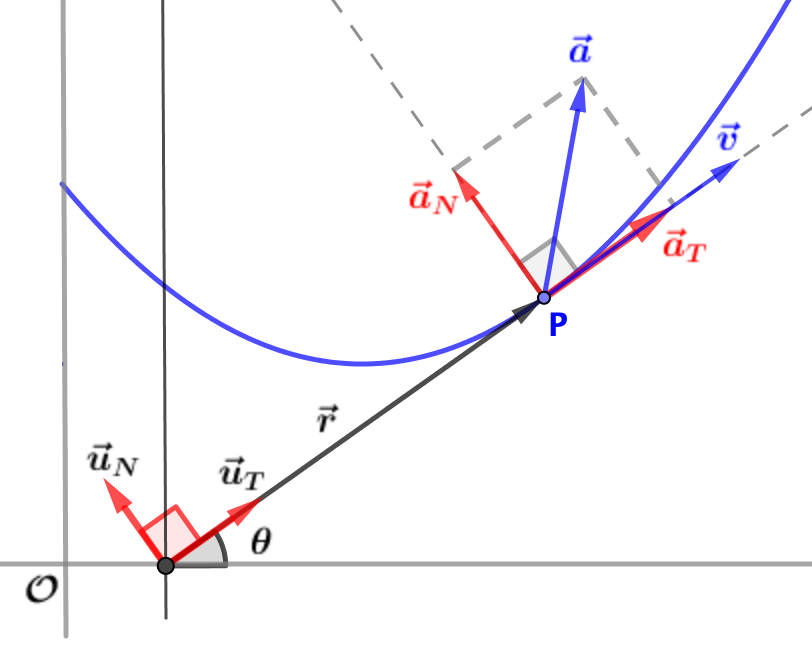
\includegraphics[width=.45\textwidth]{imagenes/imagenes02/T02IM13.png}
		\end{figure}
\end{multicols}


Al pasar de $\;t\;$ a $\;t+dt\;$, el ángulo polar cambia $\;\dd \theta=\theta(t+dt)-\theta(t)$.

Por otro lado, de la relación \emph{arco=ángulo por radio} (cuando el ángulo se expresa en radianes) tenemos:

$\dd s=\dd \theta \cdot \rho\;$ Donde $\rho$ es el llamado \emph{radio de curvatura}.

Como $\; \displaystyle \dv{\theta}{t}=\dv{\theta}{s}\cdot \dv{s}{t}=\dfrac 1 \rho \; v$ 

\begin{figure}[H]
		\centering
		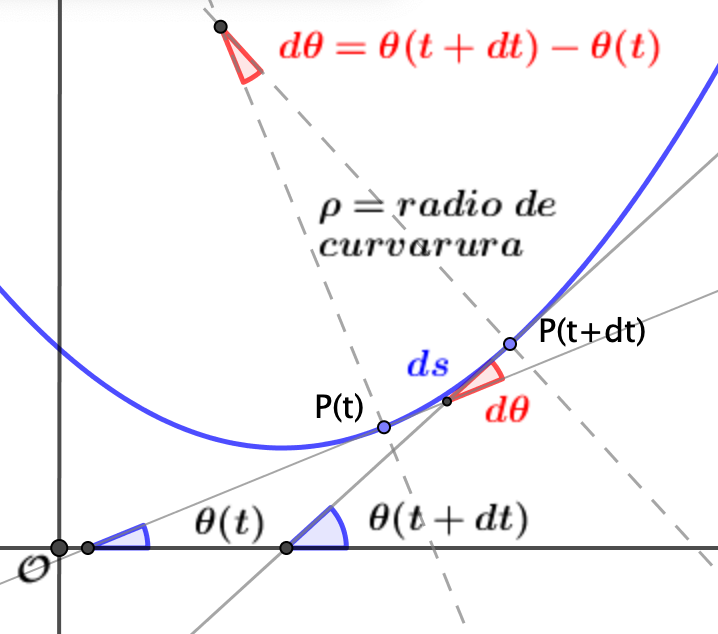
\includegraphics[width=.6\textwidth]{imagenes/imagenes02/T02IM14.png}
		\end{figure}


Se tiene que:

\begin{equation}
\subrayado{
\label{intrinsecas}
\vec a\;=\;\vec u_T\; \dv{v}{t} \;+\; \vec u_N	\; \dfrac {v^2}{\rho}
}
\end{equation}

\begin{miparrafo}

\noindent \textbf{---} La aceleración tangencial, $a_T$, mide el cambio del módulo del vector velocidad (si la partícula viaja más deprisa o más despacio) y es tangente, en todo momento, a la trayectoria.

\vspace{3mm}
\noindent \textbf{---}  La aceleración normal, $a_N$, mide el cambio de la dirección del vector velocidad y es perpendicular (normal) a la trayectoria en todo momento.

\end{miparrafo}

En coordenadas polares, el módulo del vector aceleración se mide por:
$$\displaystyle \abs{\vec a}=\sqrt{\left(\dv{v}{t} \right)^2+\dfrac {v^4}{\rho^2}}$$

-- Para MR, aquellos en los que que no cambia la dirección del vector velocidad, $a_n=0 \to \; \rho = \infty $ (recta).

-- Pra MRU, $\vec v=\overrightarrow{cte}$, tenemos $\abs{\vec v}=cte \to \displaystyle \dv{v}{t}=0 \to a_T=0$

OJO: $\displaystyle \dv{v}{t}= \dv{\abs{\vec v}}{t} \; \neq \; \abs{\dv{\vec v}{t}}$.

\begin{figure}[H]
		\centering
		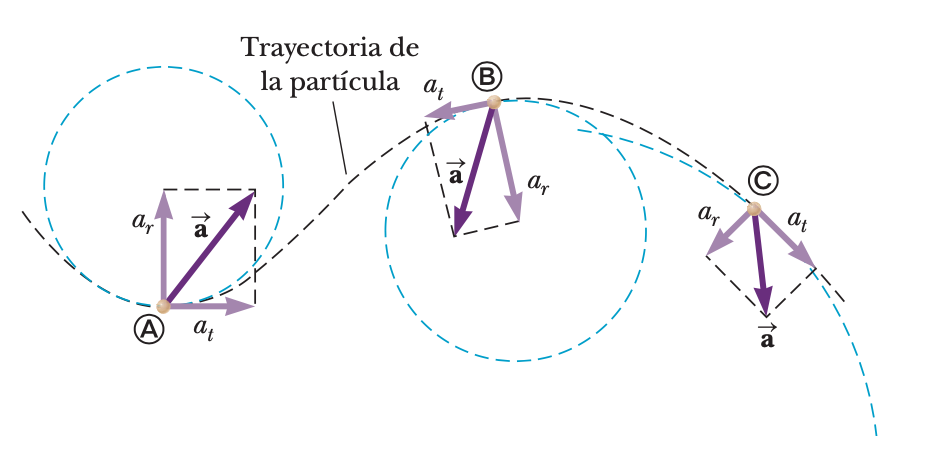
\includegraphics[width=.8\textwidth]{imagenes/imagenes02/T02IM39.png}
		\end{figure}
\vspace{-10mm} %************
\rule{150pt}{0.4pt}

\begin{multicols}{2}
ATENCIÓN: 

No confundir las componentes polares de la aceleración, en las direcciones $\vec u_r$ y $\vec u_\theta$ con las componentes intrínsecas, en las direcciones tangencial $\vec u_T$ y normal $\vec u_n$.
\begin{figure}[H]
		\centering
		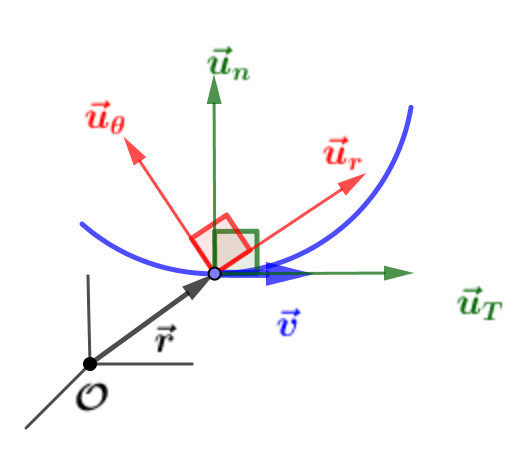
\includegraphics[width=.4\textwidth]{imagenes/imagenes02/T02IM35.png}
		\end{figure}
\end{multicols}
\vspace{-10mm} %**************************************
\rule{150pt}{0.4pt}

\textbf{Los movimientos se pueden clasificar según las componentes intrínsecas de su aceleración. }
\vspace{-2mm}\begin{enumerate}
\vspace{-2mm}\item $a_T=0$ 
	\vspace{-2mm}\begin{enumerate}
	\vspace{-2mm}\item $a_N=0$. Movimiento rectilíneo a velocidad constante. 
	\vspace{-2mm}\item $a_N=cte$. Movimiento circular uniforme. 
	\vspace{-2mm}\item $a_N\neq cte$. Movimiento circular acelerado. 
	\vspace{-2mm}\end{enumerate}
\vspace{-2mm}\item $a_N=0$ 
	\vspace{-2mm}\begin{enumerate}
	\vspace{-2mm}\item $a_T=0$.   Movimiento rectilíneo a velocidad constante. 
	\vspace{-2mm}\item $a_T=cte$. Movimiento rectilíneo uniformemente acelerado. 
	\vspace{-2mm}\item $a_T\neq cte$. Movimiento rectilíneo acelerado. 
	\end{enumerate}
\vspace{-2mm}\item  $a_N=0;\; a_T=0$.  Movimiento curvilíneo.
\end{enumerate}

\vspace{25mm} %***********************************
\begin{figure}[H]
		\centering
		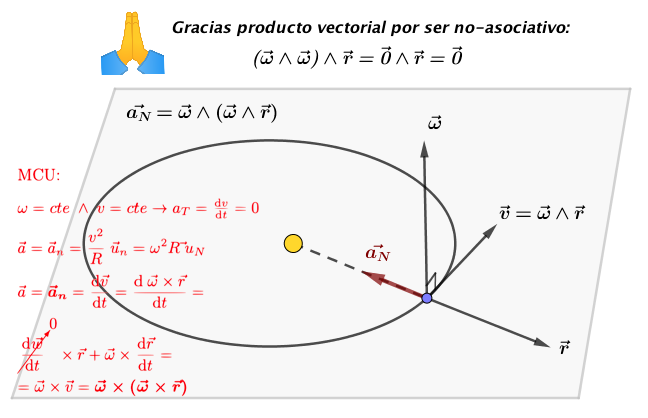
\includegraphics[width=1.1\textwidth]{imagenes/imagenes02/T02IM34.png}
		\end{figure}

\newpage %**********************
\begin{figure}[H]
		\centering
		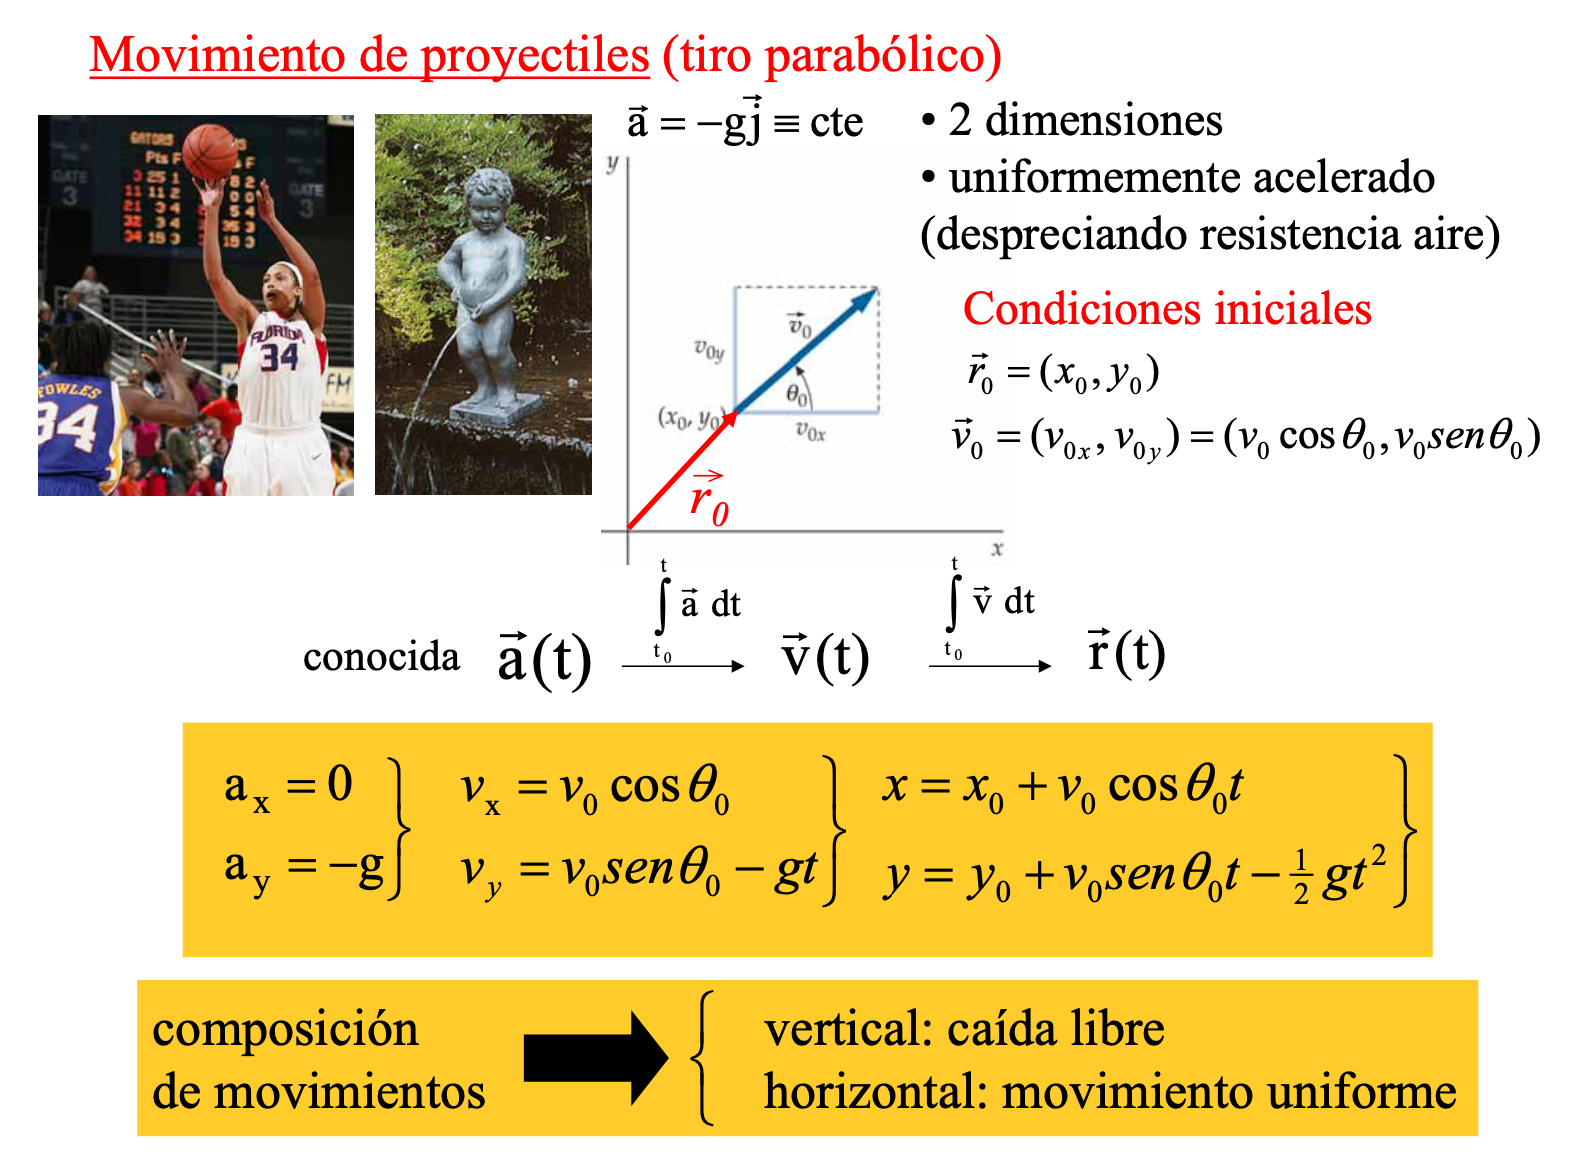
\includegraphics[width=1\textwidth]{imagenes/imagenes02/T02IM22.png}
		\end{figure}
		
\begin{figure}[H]
		\centering
		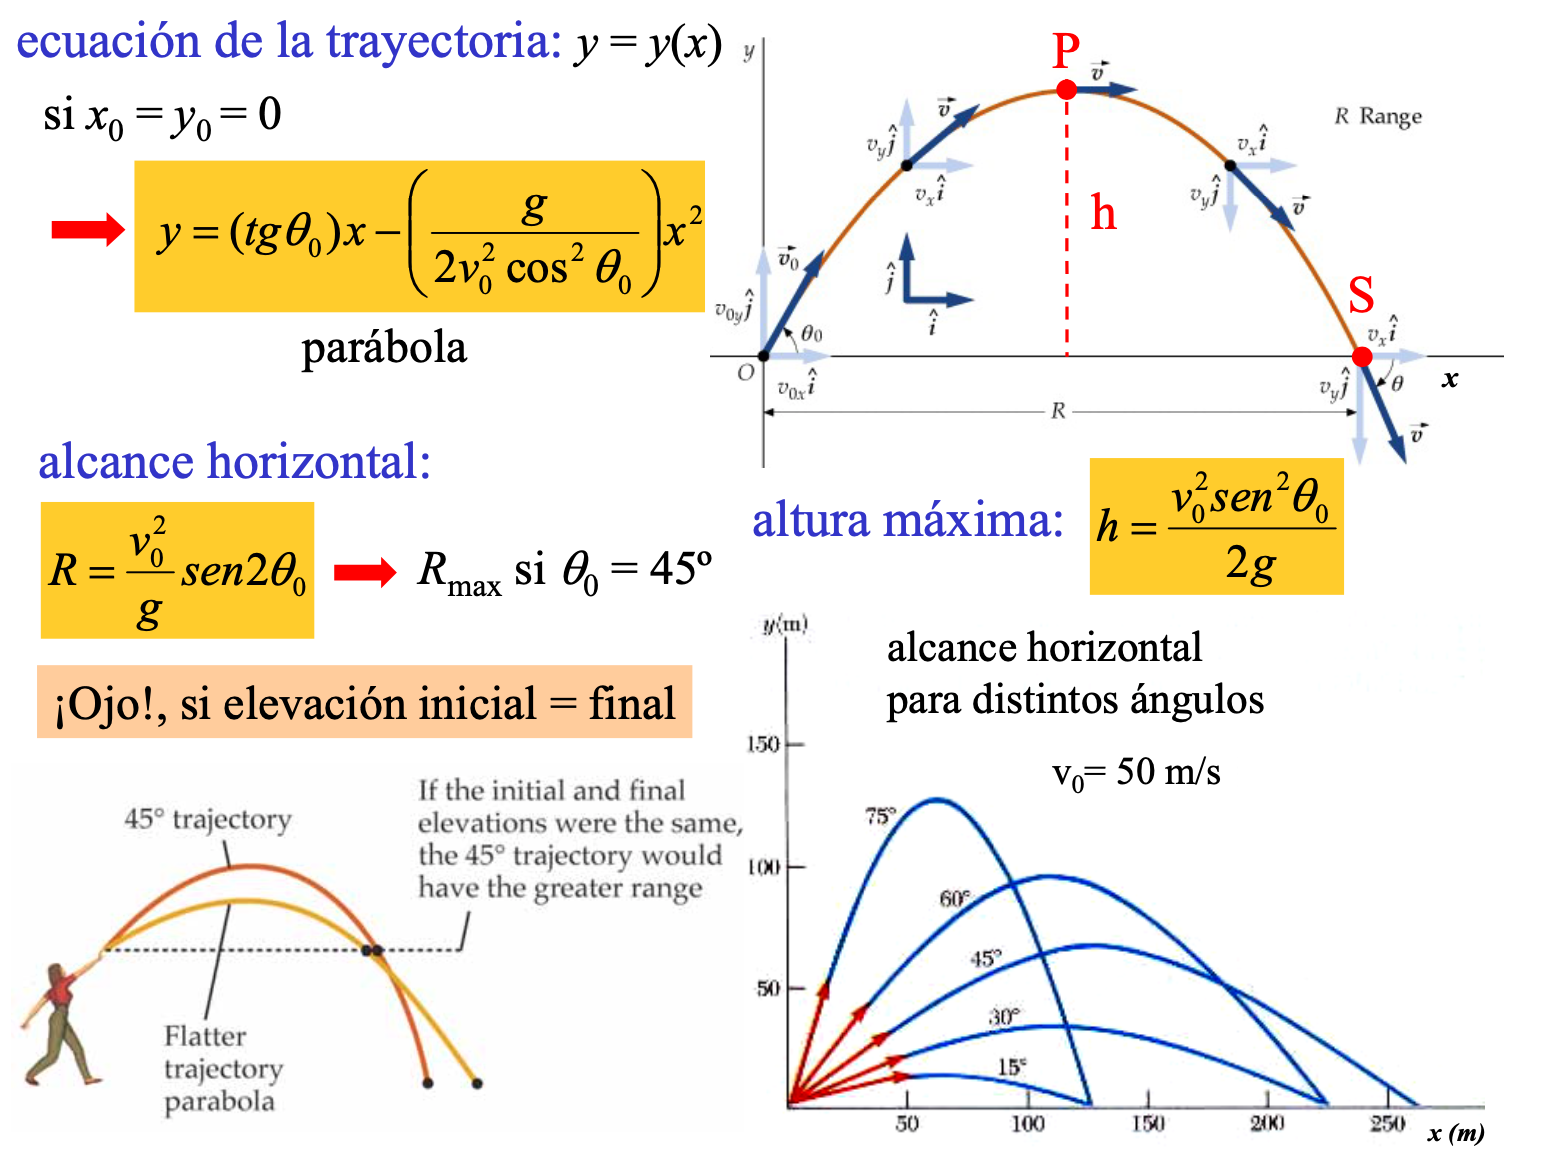
\includegraphics[width=1\textwidth]{imagenes/imagenes02/T02IM23.png}
		\end{figure}


	\begin{figure}[H]
		\centering
		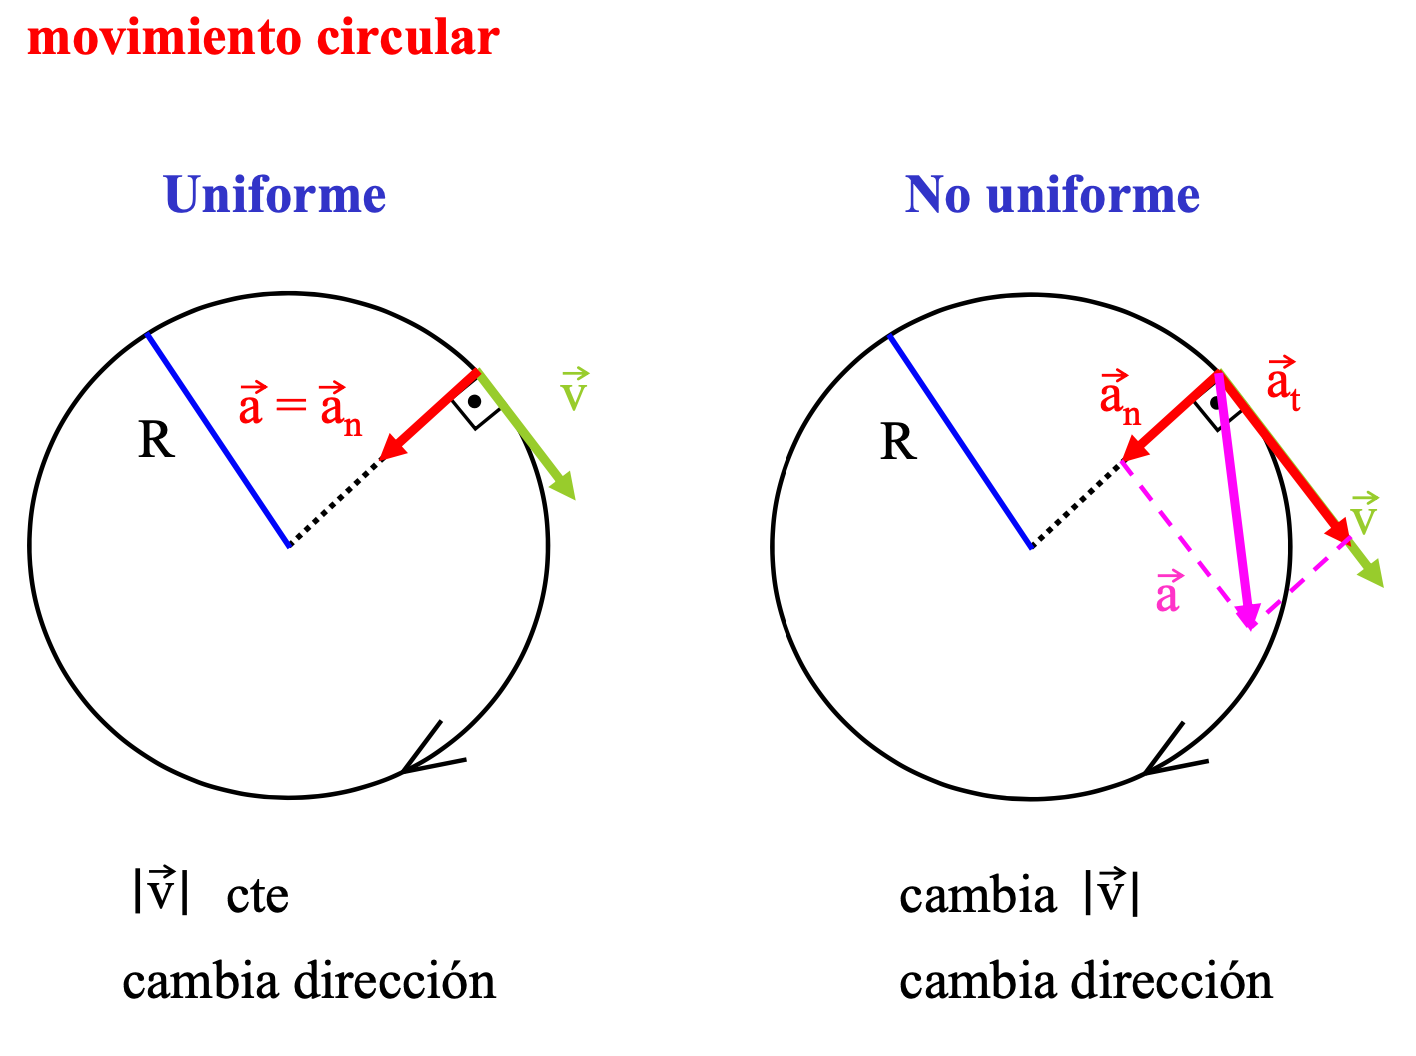
\includegraphics[width=.6\textwidth]{imagenes/imagenes02/T02IM29.png}
		\end{figure}
	\vspace{-4mm}\begin{figure}[H]
		\centering
		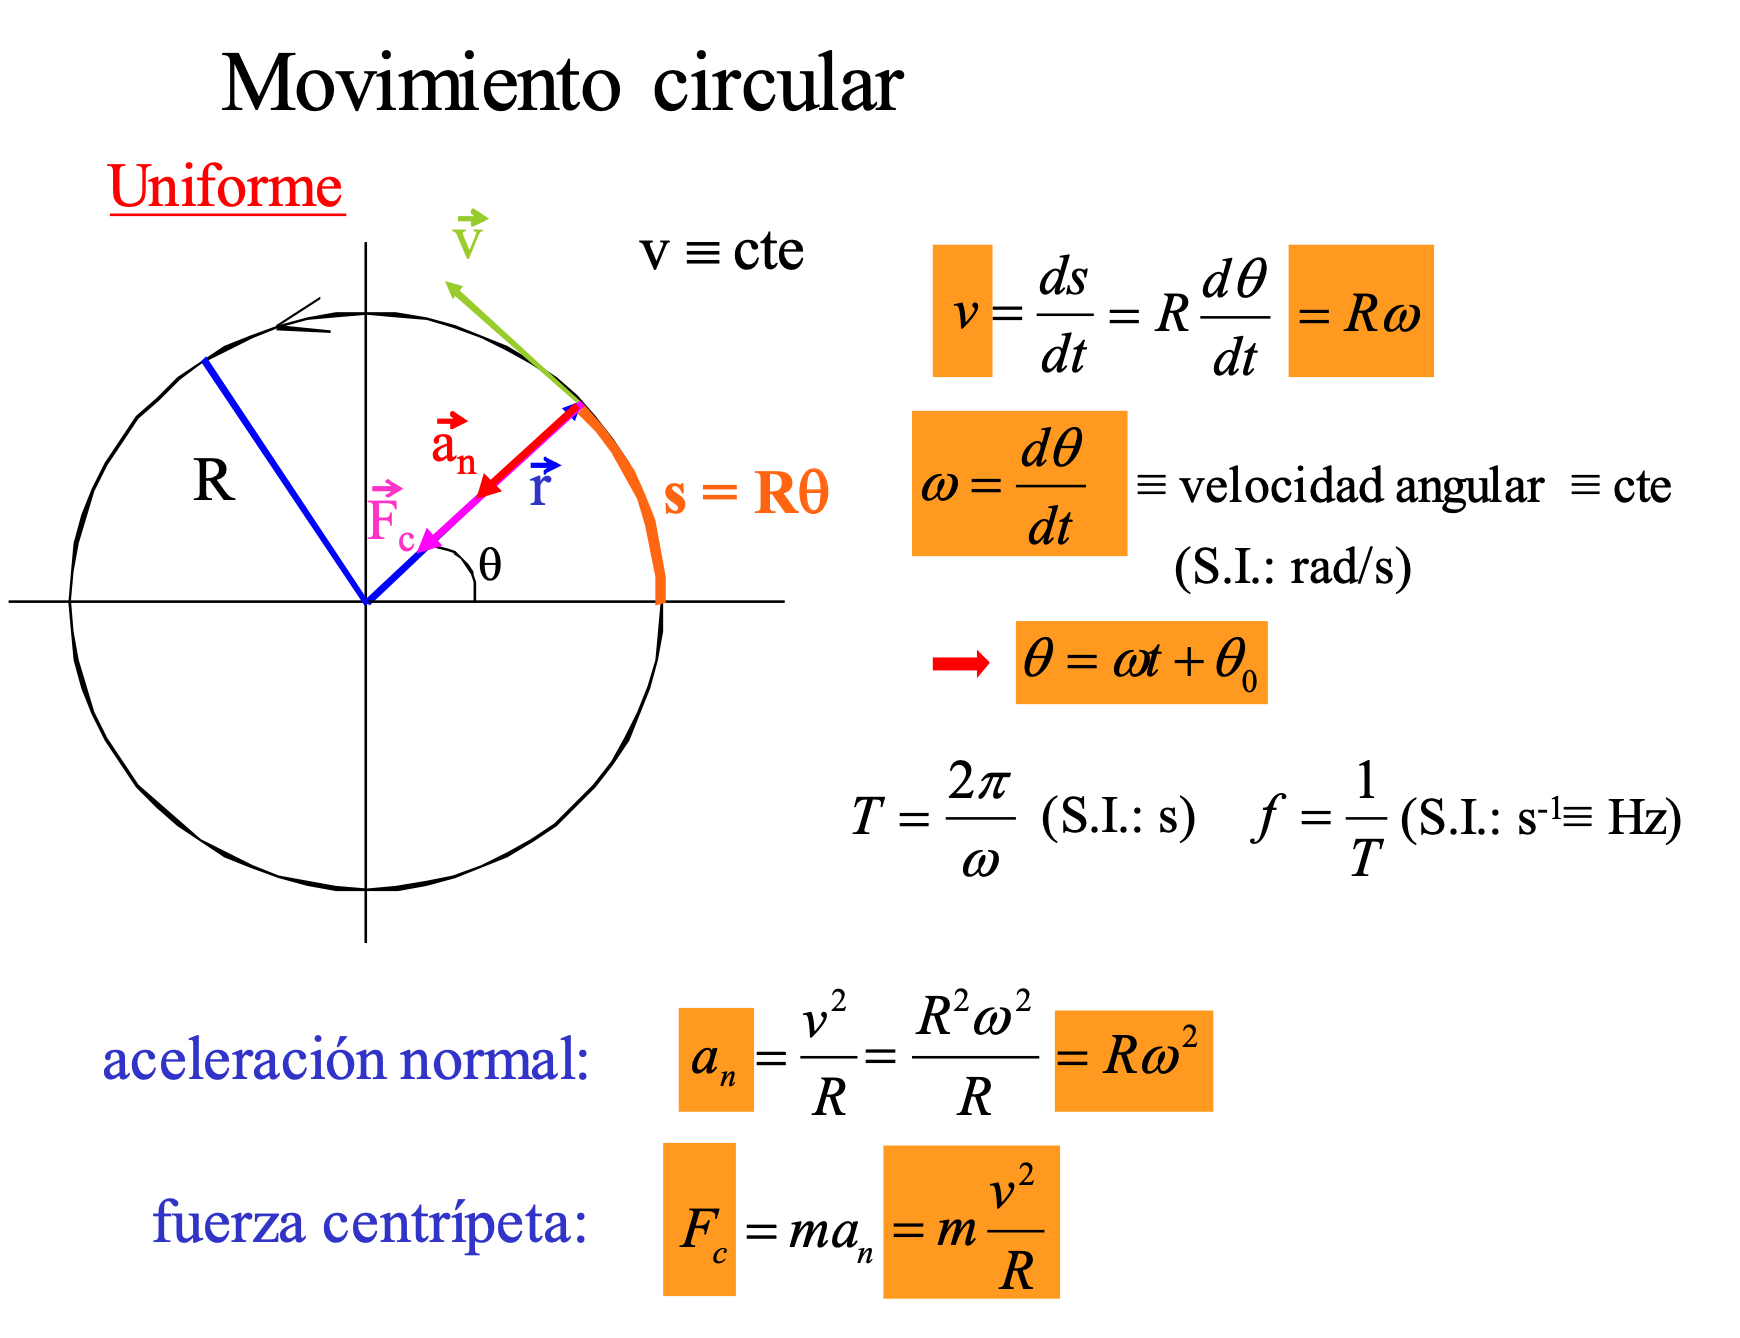
\includegraphics[width=.7\textwidth]{imagenes/imagenes02/T02IM31.png}
		\end{figure}
	\vspace{-5mm}\begin{figure}[H]
		\centering
		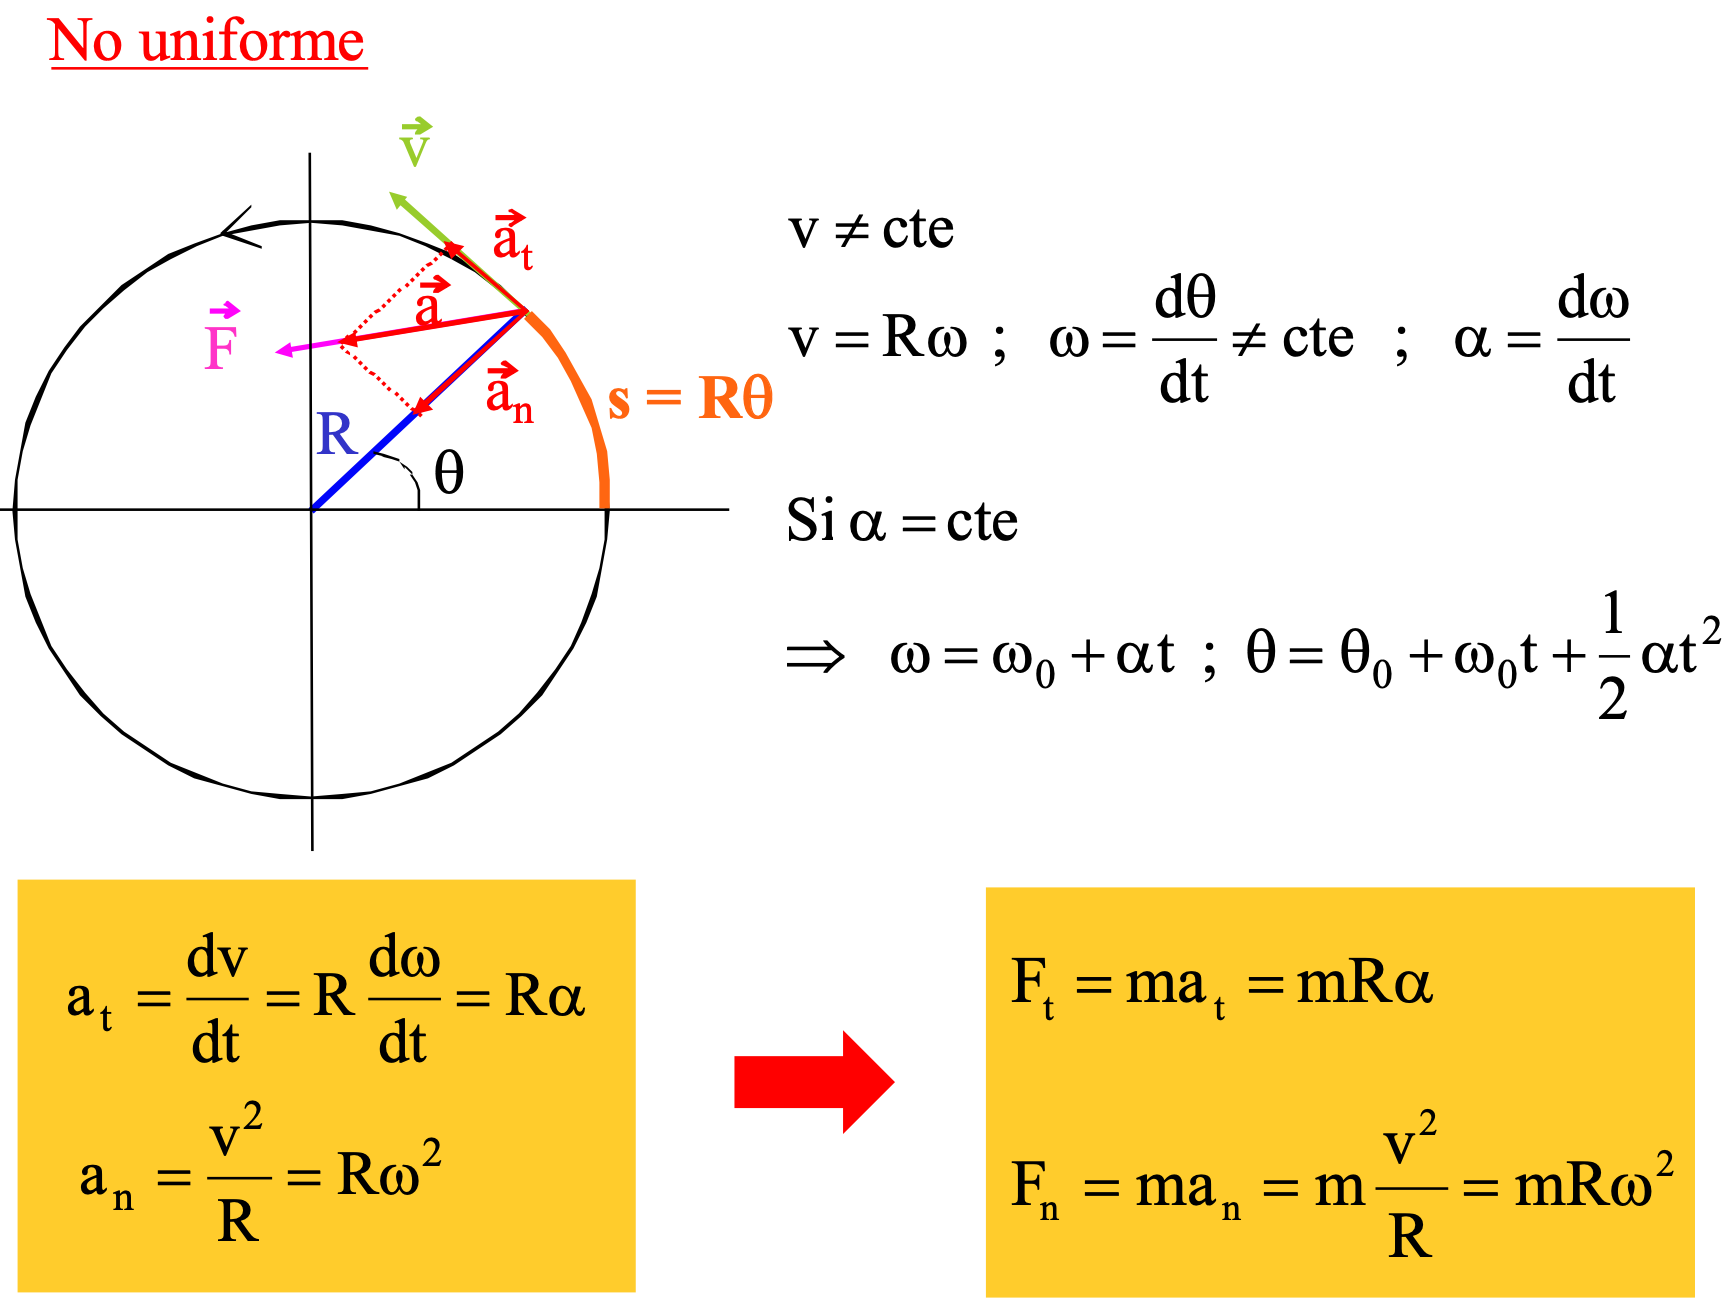
\includegraphics[width=.7\textwidth]{imagenes/imagenes02/T02IM32.png}
		\end{figure}


\section{Problemas}

\begin{prob}
Se está usando un vehículo robot para explorar la superficie de Marte. El módulo de descenso es el origen de coordenadas; en tanto que la superficie marciana circundante está en el plano $XY$. El vehículo, que representamos como un punto, tiene coordenadas x y y que varían con el tiempo según: $x=2-0.25t^2$, $y=t+0.025t^3$, estando $t$ en $\mathrm{s}$ y $x$ e $y$ en $\mathrm{m}$ 
\begin{quote}
\begin{enumerate}[a) ]
\item Obtenga las coordenadas del vehículo y su distancia con respecto al módulo en $t=2\;\mathrm{s}$ . 
\item Obtenga los vectores de desplazamiento y velocidad media del vehículo entre $t=2\;\mathrm{s}$ y $t=4\;\mathrm{s}$
\item Deduzca una expresión general para el vector de velocidad instantánea del vehículo. 
\item Exprese la velocidad instantánea en $t=2\; \mathrm{s}$ en forma de componentes y además en términos de magnitud y dirección.  
\item Obtenga el vector aceleración en cualquier instante $t$.
\item Obtenga las componentes de la aceleración en el instantes $t=2\; \mathrm{s}$. 
\item Obtenga las componentes paralela y perpendicular de la aceleración en $t = \;2 \mathrm{s}$. 
\end{enumerate}
\end{quote}	
\end{prob}
 $x=2-0.25t^2\qquad y=t+0.025t^3 \qquad t(\mathrm{s});\;\; x(\mathrm{m}),\; y(\mathrm{m})$
 
 --- a) $t=2\to x=1\;\mathrm{m};\quad y=8.2\; \mathrm{m}\; \quad \vec r=\vec i+8.2\vec j; \quad \abs{\vec r}=8.26\; \mathrm{m}$
 
 --- b) $\displaystyle \overline{\;\vec v\; }=\dfrac{\Delta \vec r}{\Delta t}=\dfrac{\vec r(4)-\vec r(2)}{4-2}$
 
$ \begin{cases}
 \vec r(4)=x(4)\; \vec i+ y(4)\vec j=-2 \vec i +9.6 \vec j
 \\
 \Delta r=(-2,9.6)-(1,8.2)=3\vec i+1.4\vec j 
\end{cases}
\displaystyle \overline{\;\vec v\; }=\dfrac {(3,1,4)}{4-2}=(\;1.5\vec i+0.7\vec j\;)\; \mathrm{ms}^{-1}$

$\abs{\displaystyle \overline{\;\vec v\; }}=\sqrt{1.5^2+0.7^2}=1.66\; \mathrm{ms}^{-1}$

--- c) $\vec v=\displaystyle\dv{\vec r}{t}= \dv{x}{t}\vec i+\dv{y}{t} \vec j= -0.5t\;\vec i + (1+0.075t^2)\;\vec j $

--- d) $t=2s \to \vec v(2)=-\vec i+1.3\; \vec j \to \abs{\vec v(2)}= 1.64\; \mathrm{ms}^{-1};\; \theta_{\vec v(2)}=\arctan \dfrac {v_y} {v_x}=127.6^o$, siendo $\theta_{\vec v(2)}$ el ángulo que forma el vector velocidad con semieje $OX+$ en el instante $t=2\; \mathrm{s}$.

--- e) $\displaystyle \vec a= \dv{\vec v}{t}=-0.5\;\vec i+ 0.15t\; \vec j$

--- f) $\vec a(2)=-0.5\;\vec i+0.3\vec j \quad \to \quad a_x=-0.5 \; ms^{-1}; \; \; a_y(2)=0.3\;\mathrm{ms}^{-2};$

$\displaystyle   \abs{\vec a(2)}= 0.58\; \mathrm{ms}^{-2};\quad \theta_{\vec a_2}=\arctan \dfrac {a_y} {a_x}=149.0^o$


--- g) A partir de los ángulos que forman los vectores $\vec v$ y $\vec a$ con el semieje $OX+$, $\theta_{\vec v}$ y $\theta_{\vec a}$ a los $t=2\; \mathrm{s}$, deducimos que el ángulo que forma el vector aceleración con la recta tangente a la trayectoria (dirección del vector velocidad) es $\theta=\theta_{\vec a(2)}-\theta_{\vec a(1)}=149.0-127.6=21.4^o$, en ese mismo instante, por lo que las componentes tangencial y normal de la aceleración son:




$a_T(2)=\abs{\vec a(2)}\; \cos \theta=0.54\; \mathrm{ms}^{-2}$
$;\quad$
$a_N(2)=\abs{\vec a(2)}\; \sin \theta=0.21\; \mathrm{ms}^{-2}$

\begin{figure}[H]
		\centering
		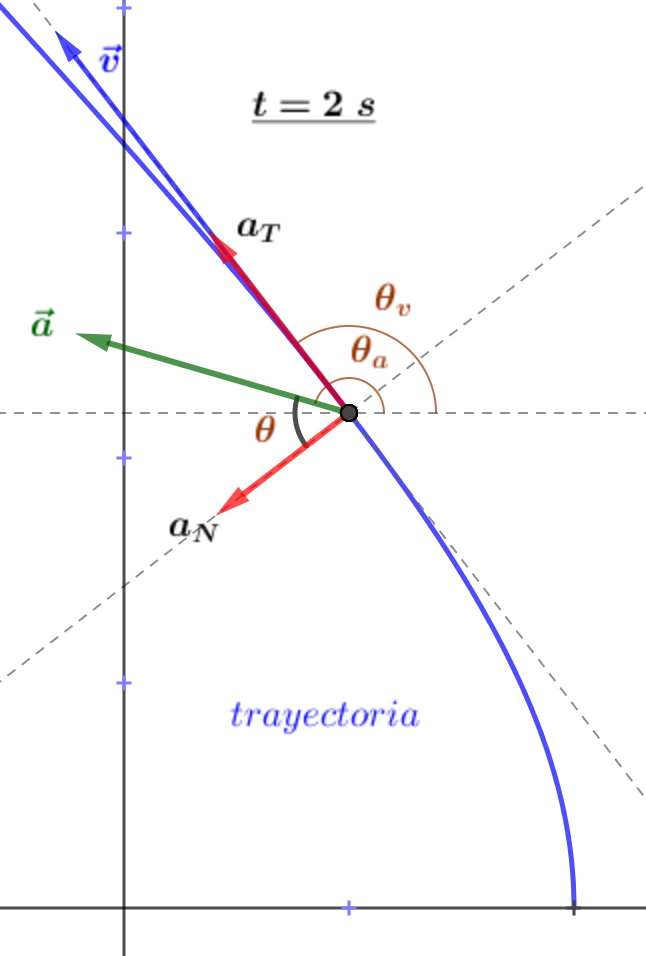
\includegraphics[width=.5\textwidth]{imagenes/imagenes02/T02IM19.png}
		\end{figure}


\begin{prob}
Una partícula se mueve en línea recta con una aceleración $a=-4v$, siendo $v$ su velocidad. Calcular la distancia que debe recorrer para que su velocidad se reduzca a $8\ \mathrm{ms}^{-1}$ y el tiempo necesario para ello si empezamos a contar cuando la velocidad de la partícula es de $80\ \mathrm{ms}^{-1}$.	
\end{prob}

$\displaystyle a=\dv{v}{t}=-4v \to \int_{v_0}^v \dfrac{\dd v}{v}=-\int_0^t 4 \dd t \to \ln \dfrac {v_0}{v}=4t \Rightarrow $ 

$\displaystyle t=\dfrac 1 4 \ln \dfrac {v_0}{v}=\dfrac 1 4 \ln \dfrac {80}{8}=0.58\ \mathrm{s}$

$\displaystyle a=\dv{v}{t}=\dv{v}{s}\ \dv{s}{t}=\dv{v}{s} \ v=-4v \to \dd v=-4 \ \dd s \to $

$\displaystyle \int_{v_0}^v
 \dd v=-4\int_0^s \dd s \to v-v_0=-4s \Rightarrow s=\dfrac 1 4 (v_0-v)=\dfrac 1 4 (80-8)=18\ \mathrm{m}$

\vspace{10mm} %********************************************
\begin{prob}
La velocidad angular de una rueda viene dada por la ecuación $\omega=2\ \theta^{1/2}$. Calcular el tiempo necesario para dar una vuelta completa así como la aceleración angular en cada instante. ?`Cómo es ese tipo de movimiento?	
\end{prob}
$\omega=\displaystyle \dv{\theta}{t}=2\ \theta^{1/2} \to \dd t=\dfrac{\dd \theta}{2\ \theta^{1/2}}=\dfrac{\dd \theta}{2\sqrt{\theta}}$

El tiempo en dar una vuelta completa, en barrer $2 \pi$ radianes, es el periodo T:

$\displaystyle T=\int_0^T \dd t=\int_0^{2 \pi} \dfrac{\dd \theta}{2\sqrt{\theta}}=\eval{\sqrt{\theta}}_0^{2 \pi}=\sqrt{2 \pi}$

Aceleración angular:

$\displaystyle \alpha= \dv{\omega}{t}=2 \frac 1 2 \theta^{-1/2} \dv{\theta}{t}=\theta^{-1/2} \ \omega =\theta^{-1/2}\ 2 \theta^{1/2}=2=cte.$ 

Como $\alpha=cte$, se trata de un MCUA (movimiento circular uniformemente acelerado).

\vspace{30mm} %********************************************

\begin{prob}
Calcúlese la velocidad angular de la tierra	
\end{prob}

\begin{multicols}{2}
Si utilizamos la relación \ref{periodo-vel-angular} $\;\omega=\dfrac {2\pi}T$ y consideramos $T=24\mathrm{h}=86400 \mathrm{s}$, cometemos un error debido al efecto que tiene la traslación de la tierra, pues al dar una vuelta completa en torno a su eje, el punto $P$ estaría en la posición $P'$ y deseamos que para definir el día vuelva a apuntar al sol, $P''$. Nos hemos pasado un ángulo $\gamma$. Como la traslación es de $365$ días aprox., $\gamma=360/365 =0.986^o\approx 0.017 \text{rad}$
\begin{figure}[H]
		\centering
		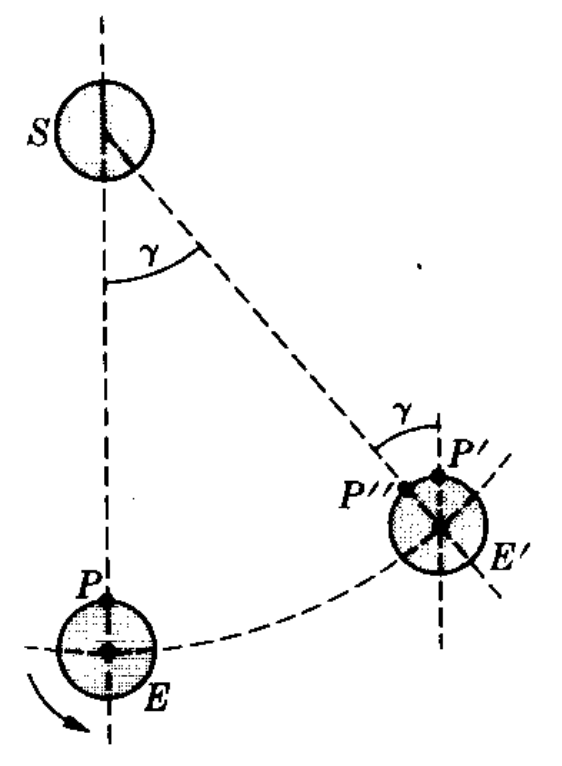
\includegraphics[width=.4\textwidth]{imagenes/imagenes02/T02IM18.png}
		\end{figure}
\end{multicols}

El tiempo $t$ aproximado para realizar ese giro por la rotación de la tierra sea corregido a  $t=\theta / \omega= 0.017 / (7.27\times 10^{-5}) \approx 234 \mathrm{s}$, donde hemos tomado como aproximación de $\omega_{rotac.}=2\pi / (24 \text{ días})=7.27\times 10^{-5}\; \mathrm{s}^{-1}$.

Esto hace que el periodo de rotación de la tierra sea $T=24horas - 234 s= 86400-234=86166\; \mathrm{s}$, con lo que:
$$\omega=\displaystyle \dfrac {2\pi}T=7.29\; \mathrm{s}^{-1}$$

\begin{prob}.

	\begin{multicols}{2}
La Tierra rota uniformemente respecto a su eje con una velocidad angular $\;\omega=7.3 \times 10^{-5}\;\mathrm{s}^{-1}\;$ (1 vuelta cada día). Encontrar, en función de la latitud, la velocidad y la aceleración de un punto situado en la superficie terrestre.
\begin{figure}[H]
		\centering
		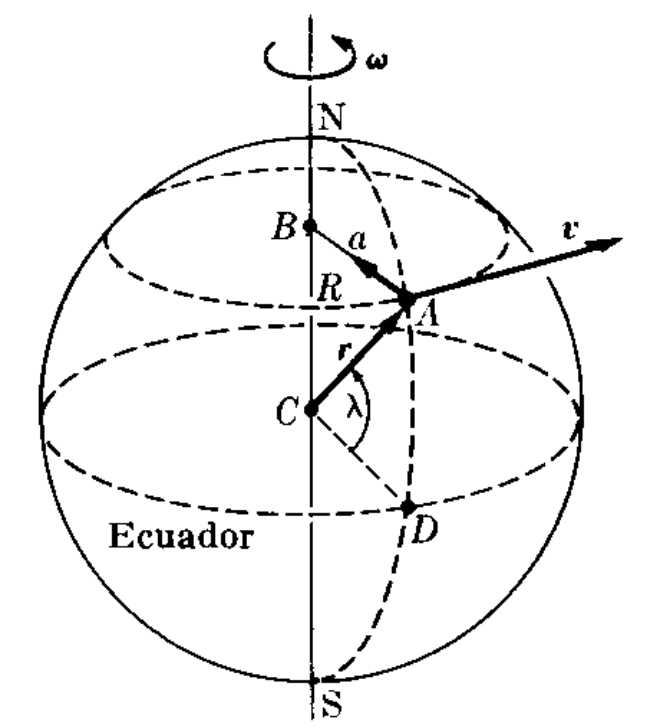
\includegraphics[width=.35\textwidth]{imagenes/imagenes02/T02IM17.png}
		\end{figure}
\end{multicols}
\end{prob}

Todos los puntos de la tierra se mueven con MRU, movimiento rectilíneo y uniforme ($\vec \omega =\overrightarrow{cte}$), luego $a_T=0$, solo hay $a_N$.

En la figura se observa que un punto A, situado a una latitud $\lambda$, describe una circunferencia paralela al ecuador de radio $r=R\; \cos \lambda$, con $R=\text{radio tierra}=6.4\times 10^6\; \mathrm{m}$.
El vector velocidad es tangente al paralelo $\lambda$, por tanto, paralelo al plano ecuatorial.

De  \ref{v-angular}: $\;\;\;v=\omega \cdot r =\omega\cdot R\cdot \cos \lambda$

De \ref{intrinsecas}: $\;\;a=a_N=\displaystyle \dfrac {v^2}r=\dfrac {\omega^2 \cdot r^2}r=\omega^2\cdot r=\omega\cdot R \cdot \cos \lambda$

Ambos valores máximos se alcanzan en el ecuador, $\lambda=0$:
$v_{max}(\lambda=0)=467 \;\mathrm{ms}^{-1}=1681.2\; \mathrm{kmh}^{-1}; \qquad a=3.4\times 10^{-2} \; \mathrm{ms}^{-2} \sim 0.3\%\; g$

\vspace{10mm} %*************************************
\begin{prob}.
	\begin{figure}[H]
		\centering
		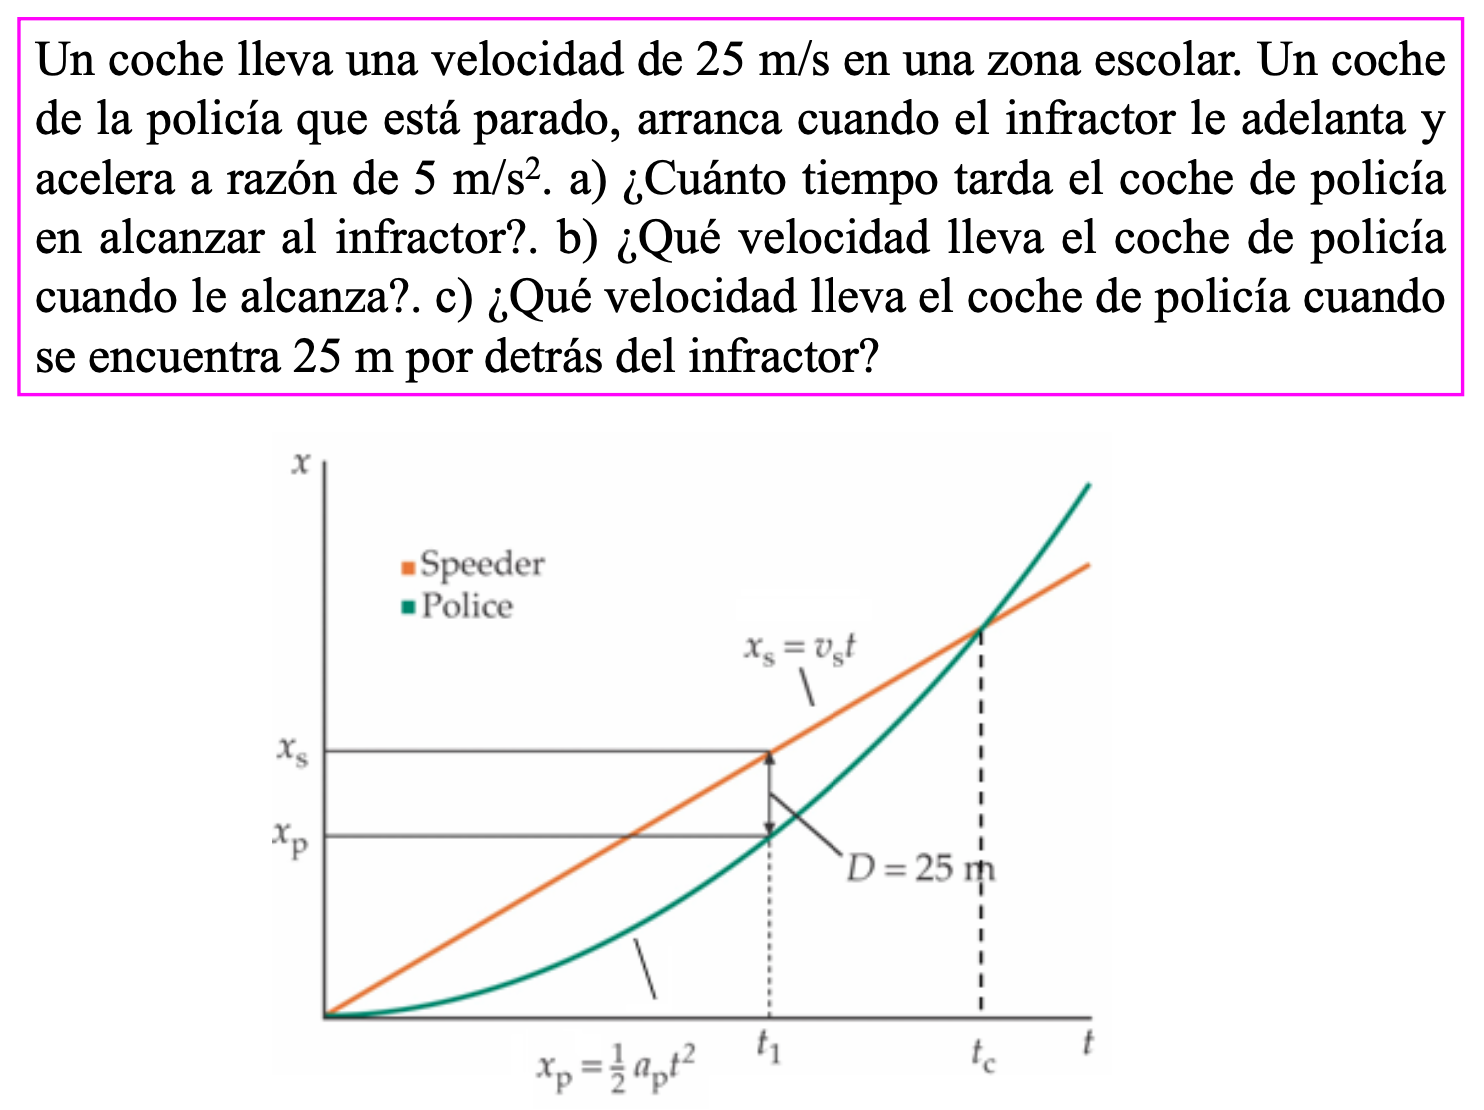
\includegraphics[width=1\textwidth]{imagenes/imagenes02/T02IM25.png}
		\end{figure}
\end{prob}

\vspace{10mm} %*************************************
\begin{prob}
Una esquiadora se mueve sobre una rampa de salto, como se muestra en la figura. La rampa es recta entre A y C, y es curva a partir de C. La rapidez de la esquiadora aumenta al moverse pendiente abajo de A a E, donde su rapidez es máxima, disminuyendo a partir de ahí. Dibuje la dirección del vector de aceleración en los puntos B, D, E y F	
\end{prob}
\begin{figure}[H]
		\centering
		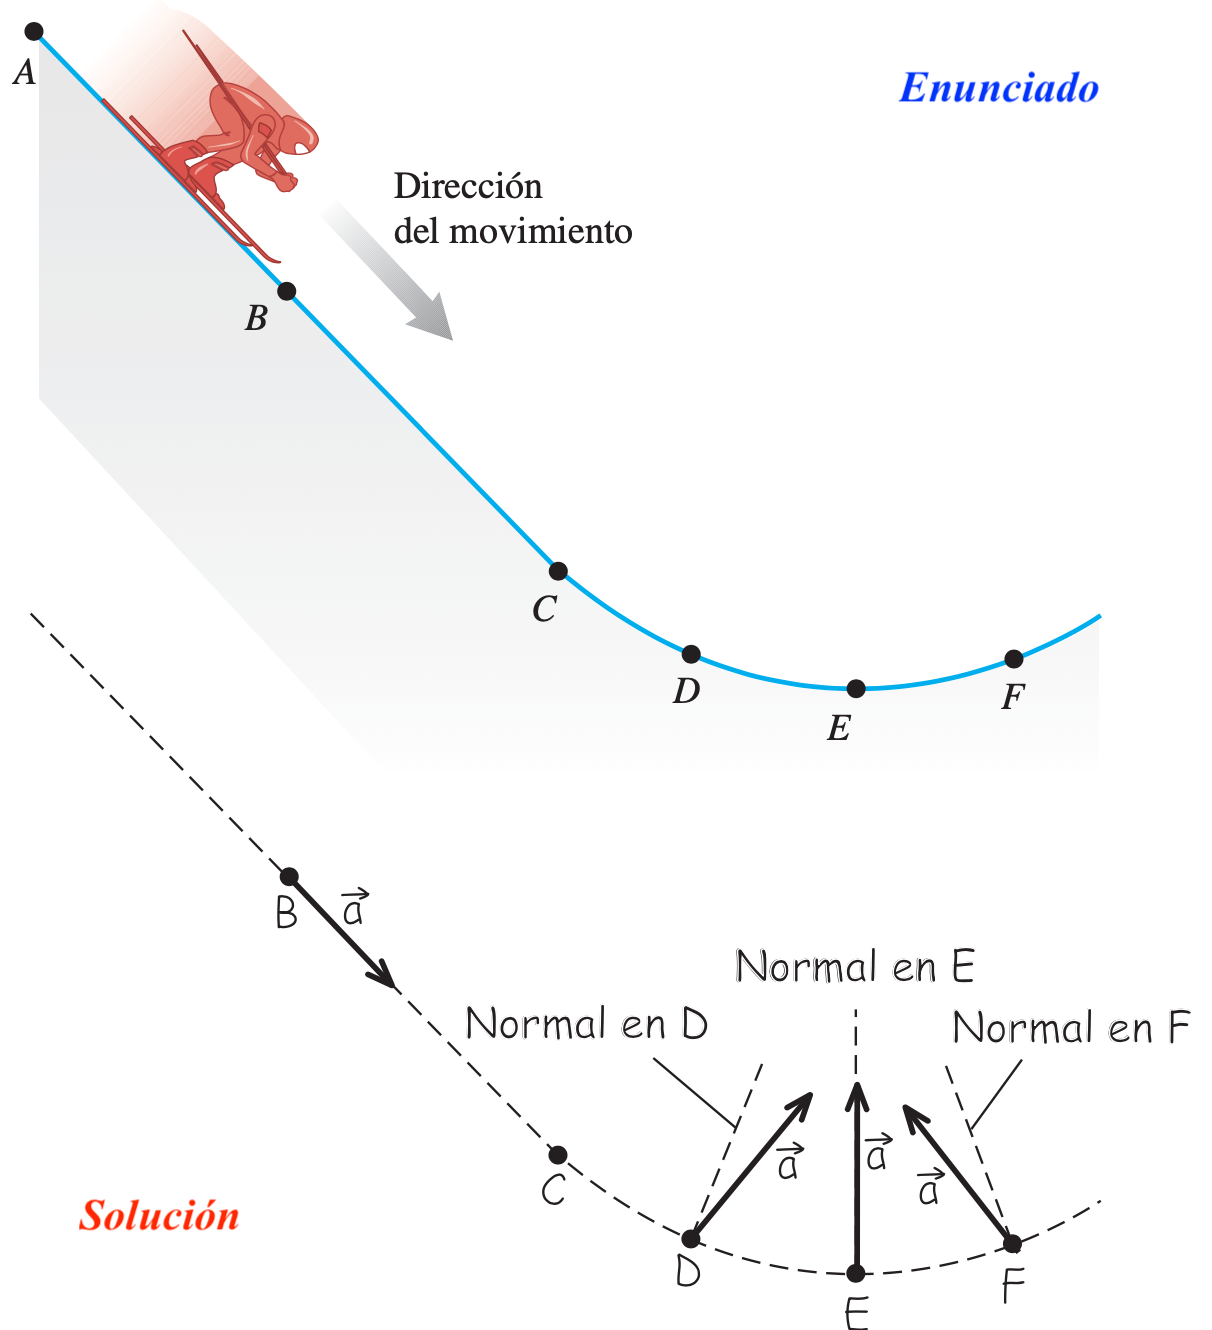
\includegraphics[width=1\textwidth]{imagenes/imagenes02/T02IM16.png}
		\end{figure}

\vspace{30mm} %*************************************

\begin{prob}.
	\begin{figure}[H]
		\centering
		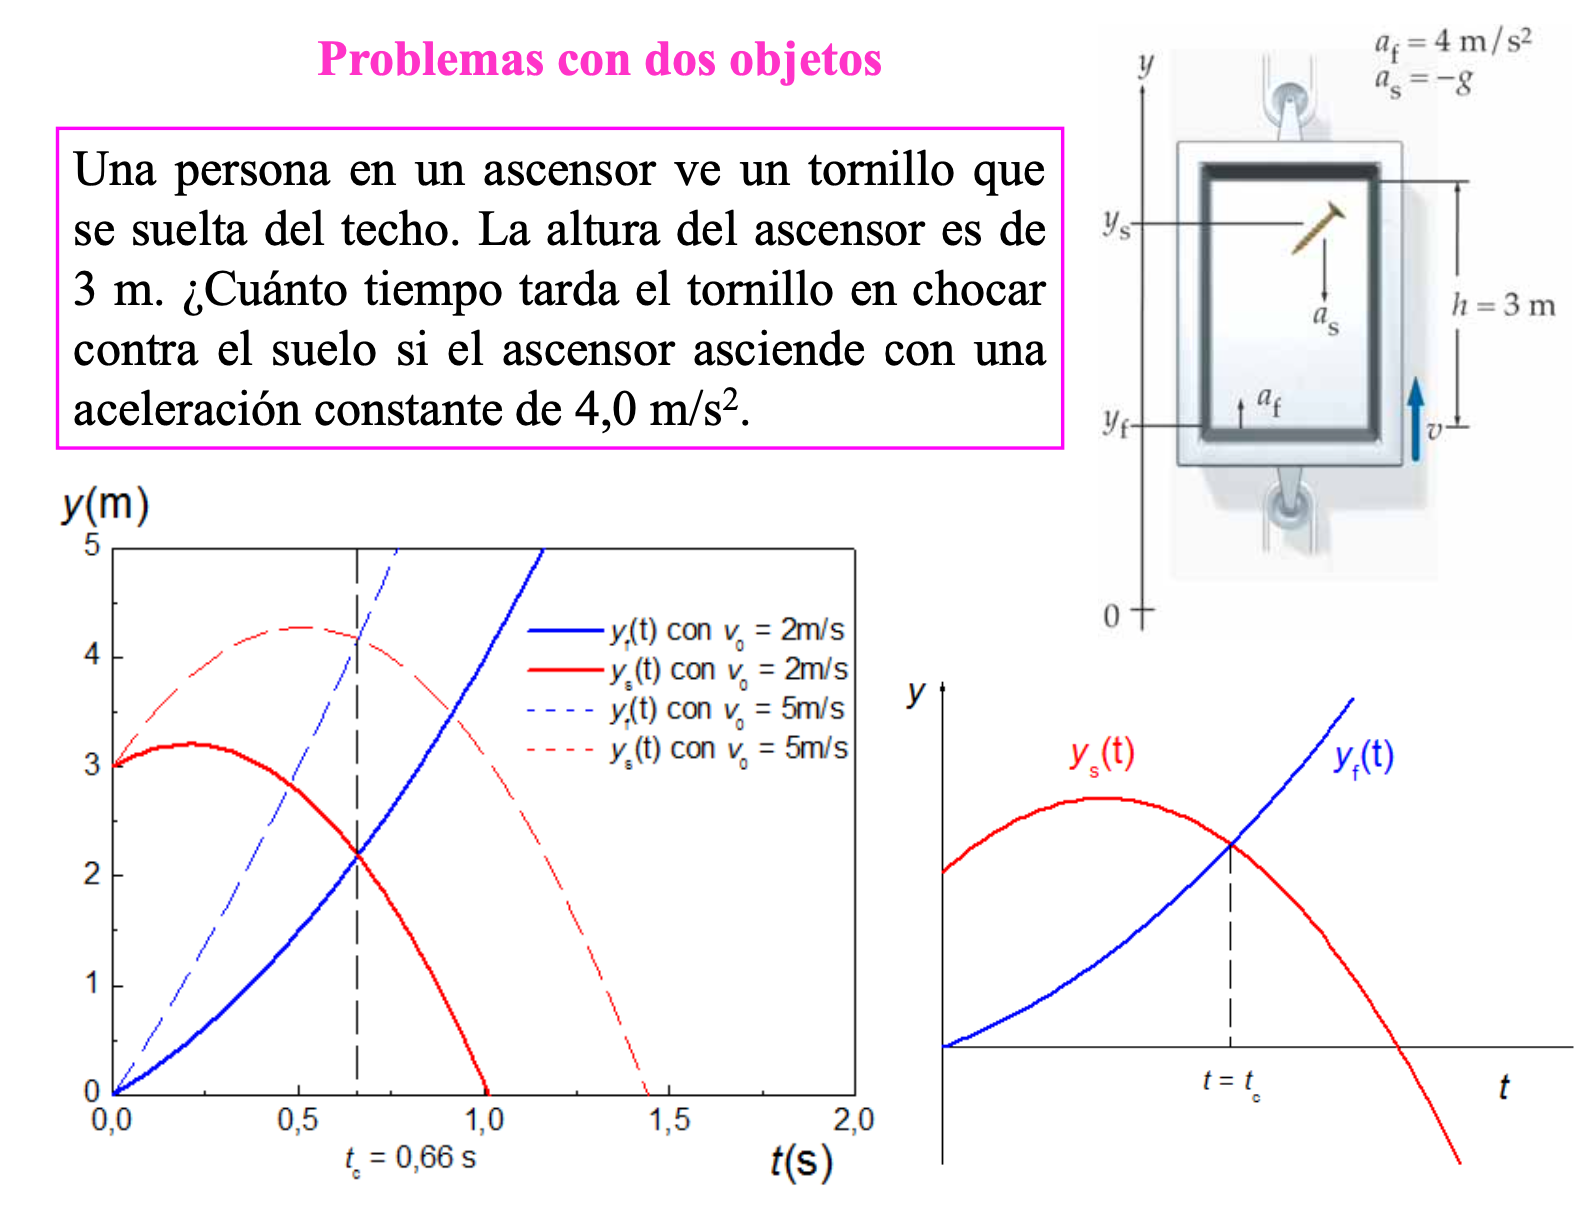
\includegraphics[width=.9\textwidth]{imagenes/imagenes02/T02IM26.png}
		\end{figure}
\end{prob}

\begin{prob}.
	\begin{figure}[H]
		\centering
		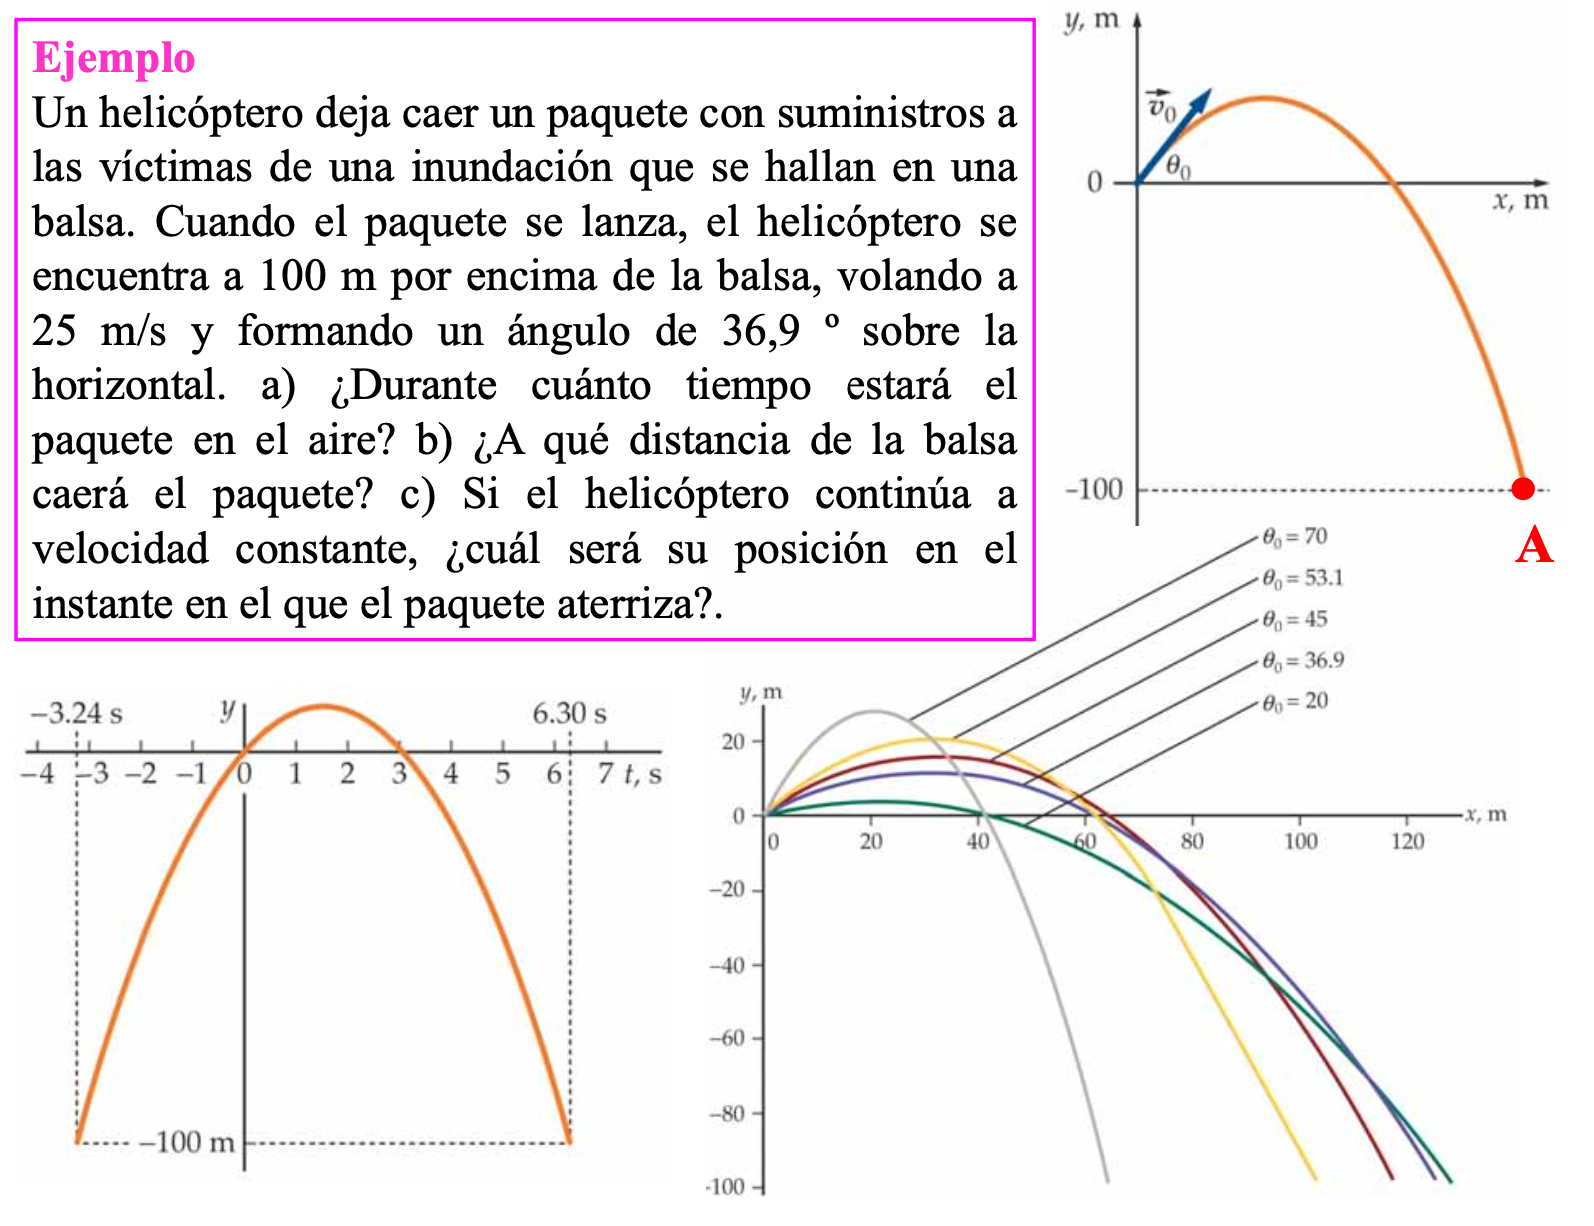
\includegraphics[width=.85\textwidth]{imagenes/imagenes02/T02IM27.png}
		\end{figure}
\end{prob}



\begin{prob} Tiro oblicuo.
\end{prob}	

\vspace{-5mm} \begin{figure}[H]
		\centering
		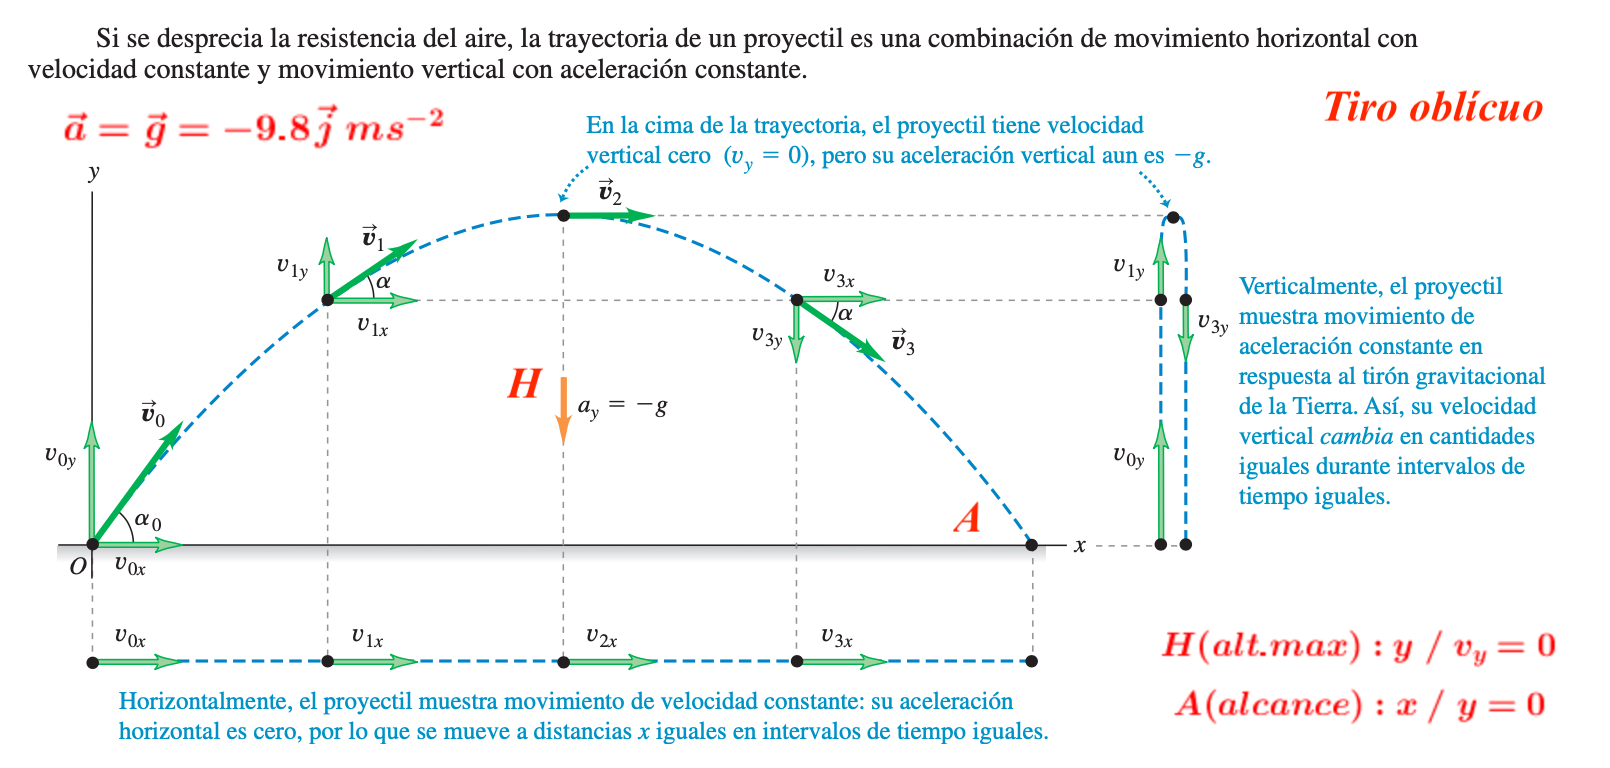
\includegraphics[width=1.1\textwidth]{imagenes/imagenes02/T02IM20.png}
		\end{figure}
		
\begin{prob} Un cazador dispara a un mono colgado de una rama. Demostrar que si el mono quiere vivir, no debe soltarse de la rama en el momento del disparo.
\end{prob}	
\begin{figure}[H]
		\centering
		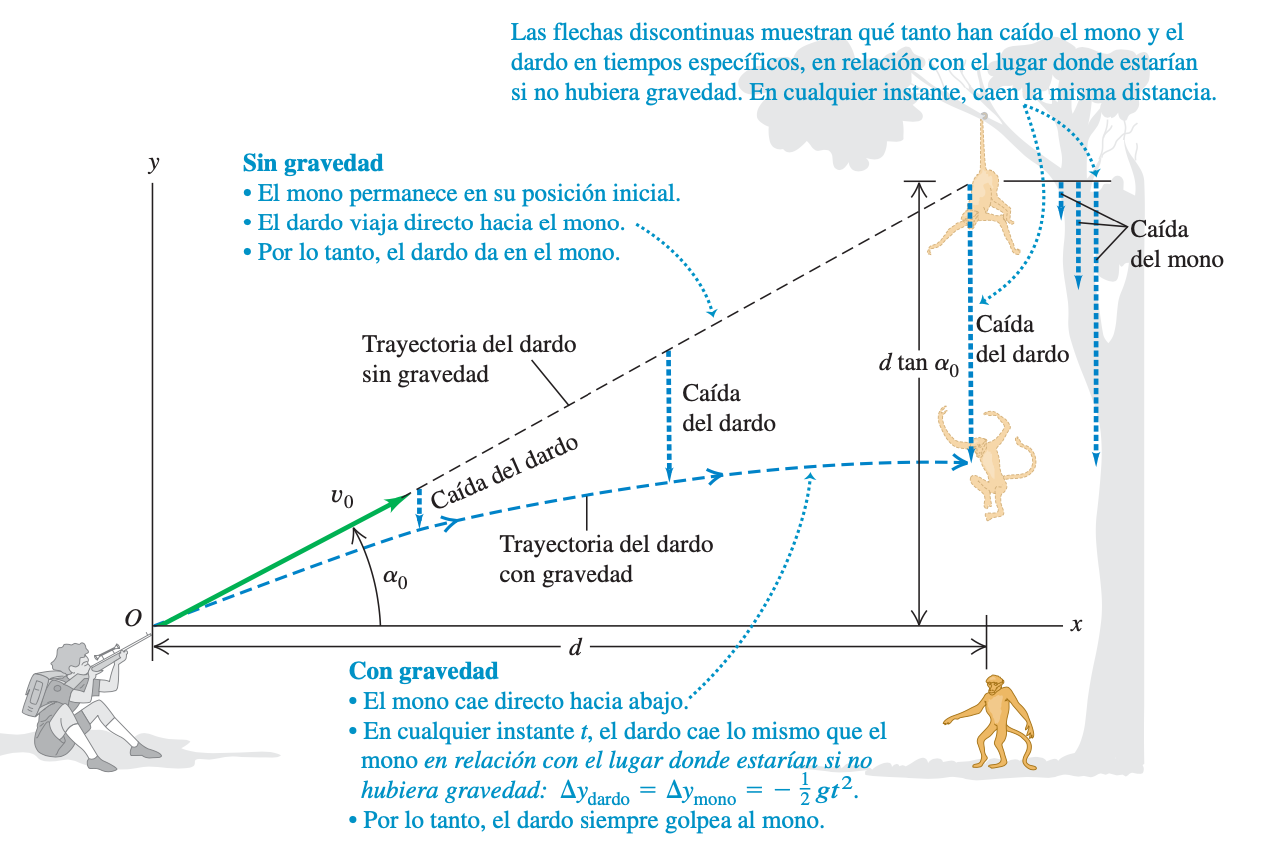
\includegraphics[width=1\textwidth]{imagenes/imagenes02/T02IM21.png}
		\end{figure}		





\begin{prob}
Una muchacha que está a $4\;\mathrm{m}$ de una pared vertical lanza contra ella una pelota que sale de su mano que está a $2 \; \mathrm{m}$ del suelo a una velocidad de $10\;\mathrm{ms}^{-1}$ y formando un ángulo de $45^o$ con la horizontal. Cuando la pelota choca contra la pared, se invierte la componente horizontal de la velocidad (rebote) mientras	 que su componente vertical continua sin variar. ¿Dónde caerá la pelota al suelo?

Comprobar que se puede considerar que la pared actúa como un espejo por lo que se puede resolver el problema como si no estuviese, calcular el alcance y, luego, considerar la reflexión especular de este punto respecto de la pared.
\end{prob}
\begin{figure}[H]
		\centering
		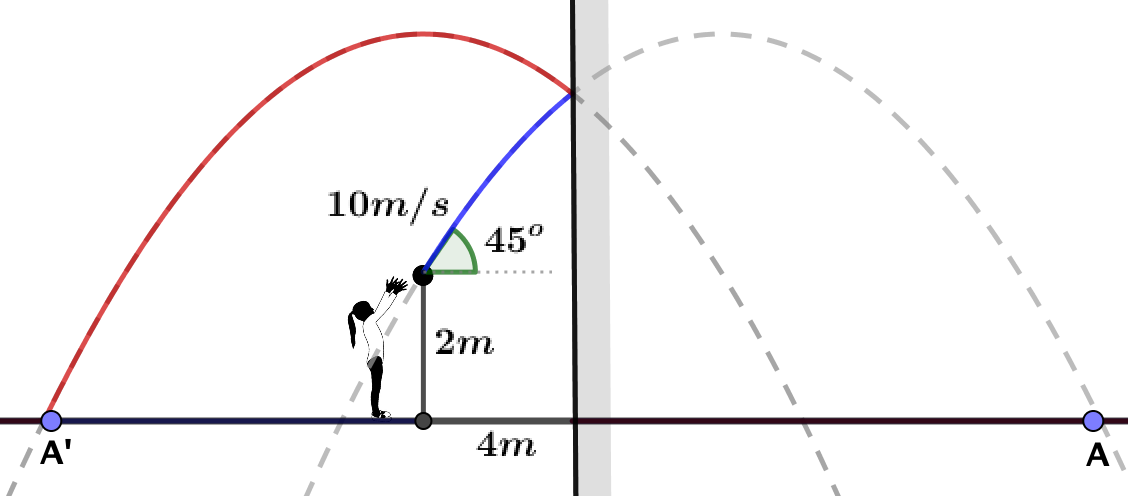
\includegraphics[width=.9\textwidth]{imagenes/imagenes02/T02IM24.png}
		\end{figure}
Dividimos el problema en dos: I- Desde el momento del tiro hasta que llega a la pared, y II- desde el rebote en la pared hasta que la pelota llega al suelo.

--- Parte I:  Colocamos el sistema de referencia en los pies de la niña u empezamos a contar el tiempo en el momento del lanzamiento, por tanto: $t_0=0\;\; x_0=0;\; y_0=2;\; v_{0_x}=v_x=v\cos \theta=10\cos 45^o=7.07;\; v_{0_y}=v\sin \theta=10\sin 45^o=7.07;\; a=g=-9.8\vec j\;$ Todo el el SI de unidades.

Cuando la pelota llega a la pared la distancia recorrida en el eje $X$ es de $4\;m$, el tiempo empleado es: $x=x_0+v_x\;t \to 4=0+7.07t \Rightarrow t=0.57\; \mathrm{s}$

Con el paso de este tiempo, calculamos la altura que ha alcanzado la pelota: $y=y_0+v_{0_y}\;t+\frac 1 2 \;a\;t^2 \to y=2+7.07\cdot 0.57-4.9\cdot 0.57^2 \Rightarrow y=4.44\; \mathrm{m}$

Calculemos, finalmente, la velocidad que lleva en su componente $y$ en ese momento: $v_y=v_{0_y}+a\; t \to v_y=7.07-9.8\cdot 0.57=1.48\; \mathrm{ms}^{-1}$

--- Parte II: Dejamos el sistema de referencia espacial a los pies de la niña pero vamos a cambiar, para facilitar el cálculo, el sistema de referencia temporal. Ahora empezamos a contar el tiempo en el momento del rebote en que se invierte el sentido de la componente $x$ del vector velocidad. Tendremos, pues: $t_0=0;\; x_0=4;\; y_0=4.44;\; v_{0_x}=v_x=-7.07;\; v_{0_y}=1.48;\; a=g=-9.8\vec j\;$, como antes, todo en el SI de unidades.

Calculemos el tiempo en que la pelota cae al suelo (desde el rebote). Eso ocurrirá cuando $y=0\to 0=4.44+1.48t-4.9t^2\Rightarrow t=1.11\; \mathrm{s}$.

Calculemos ahora la distancia recorrida durante ese tiempo por la pelota a lo largo del eje $x$: $\;x=4-7.07\cdot 1.11\approx -3.9\;\mathrm{m}$

CONCLUSIÓN: La pelota cae a $3.9\;\mathrm{m}$ a la izquierda de los pies de la niña.

\rule{150pt}{0.4pt} 

Resolvamos el problema suponiendo que la pared es un espejo. Inicialmente actuaremos como si no estuviese y, luego, calcularemos el punto simétrico del de impacto respecto de la pared-espejo.

De nuevo, colocamos el sistema de referencia en los pies de la niña u empezamos a contar el tiempo en el momento del lanzamiento, por tanto: $t_0=0\;\; x_0=0;\; y_0=2;\; v_{0_x}=v_x=v\cos \theta=10\cos 45^o=7.07;\; v_{0_y}=v\sin \theta=10\sin 45^o=7.07;\; a=g=-9.8\vec j\;$ Todo el el SI de unidades.

El tiempo de vuelo del proyectil lo encontraremos exigiendo que $y=0 \to y=y_0+v_{0_y}t+\frac 1 2 a t^2 \to 0=2+7.07t-4.9t^2 \Rightarrow t=1.69\;\mathrm{s}$

Con este tiempo, vamos a calcular el alcance de la pelota, la distancia recorrida en el eje $x$: $\; x=x_0+v_xt\to x=0+7.07\cdot 1.69=11.9\;\mathrm{m}$

Es decir, si no hay pared-espejo, la pelota cea a $11.9\;\mathrm{m}$ de los pies de la niña, es decir, a $11.9-4=7.9\;\mathrm{m}$ de la pared.  El simétrico de $+7.9\;\mathrm{m}$ de la pared es $-7,9\;\mathrm{m}$ de la misma, es decir, a su izquierda. Como la niña está a $4\:\mathrm{m}$ a la izquierda de la pared, la pelota caerá, pues, a $7.9-4=3.9\;\mathrm{m}$ a la izquierda de la niña.

\begin{prob}
Conduces un automóvil por una autopista recta. En el instante $t = 0$, cuando avanzas a $10 \ \mathrm{ms}^{-1}$ en la dirección $+x$, pasas un letrero que está en $x= 50 \ \mathrm{m}$. Tu aceleración es una función del tiempo: $_x = (2.0 - 0.10 t)\ \mathrm{ms}^{-2}$. 

a) Deduce las expresiones para tu velocidad y posición en función del tiempo.  

b) ¿En qué momento es máxima tu velocidad?  

c) ¿Cuál es esa velocidad máxima?  
\end{prob}
$v=10+2t-0.05t^2$ 

$x=50+10t+t^2-0.017t^3$

$a=0$ si $t=20 \to v_{max}=30\ \mathrm{ms}^{-1}$	

\begin{prob}
Sabemos demostrar que, en ausencia de rozamiento con el aire, el alcance máximo de un cuerpo que sigue un movimiento parabólico se consigue para un lanzamiento a $45^o$ sobre la horizontal (siempre que el punto de lanzamiento y el de impacto se encuentren a la misma altura). ¿Es también cierto cuando el suelo está inclinado? 
\end{prob}
\begin{multicols}{2}
Datos: $\vec v_0,\;\; \theta,\;\; \phi$

A encontrar $d=d(\vec v_0,\theta,\phi)$

Para $v_0, \ \theta \ { y }\  \phi$ dados $\to d_{max}(\phi)$
\begin{figure}[H]
		\centering
		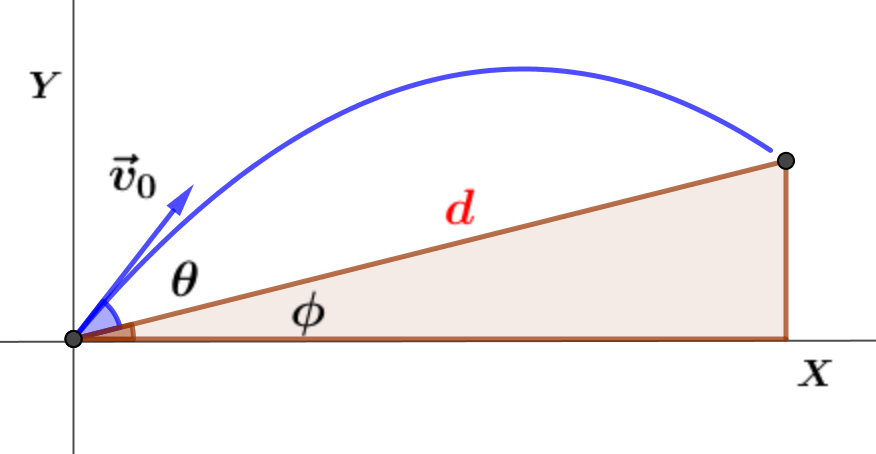
\includegraphics[width=.5\textwidth]{imagenes/imagenes02/T02IM36.png}
		\end{figure}
\end{multicols}

Sistema de referencia en punto de lanzamiento y empezamos a contar el tiempo en el momento del mismo: $x_0=y_0=t=0$.

Buscamos la ecuación de la trayectoria parabólica que describe el proyectil. Partimos de las ecuaciones de las posiciones:

$\begin{cases} x=v_0 \cos (\theta+\phi) \ t \\ y=v_0 \sin (\theta+\phi) \ t - \frac g 2 t^2 \end{cases}  \to t=\dfrac x{v_0 \cos (\theta+\phi)} $

$\Rightarrow y=\cancel{v_0} \sin (\theta+\phi) \dfrac x{\cancel{v_0} \cos (\theta+\phi)} - \dfrac g 2 \left( \dfrac x{v_0 \cos (\theta+\phi)}  \right)^2$

La ecuación de la trayectoria (parábola) es:

$\textcolor{blue}{y=\tan(\theta+\phi) \ x - \dfrac {g}{2 v_0^2 \cos^2 (\theta+\phi)}\ x^2}$

Por otra parte, la ecuación del plano inclinado es:

$\textcolor{red}{y}=mx\textcolor{red}{=\tan \phi \ x}$

El punto de impacto del \textcolor{blue}{proyectil} contra el \textcolor{red}{suelo} se producirá en la \textbf{intersección} de la \textcolor{blue}{parábola (trayectoria)} con la \textcolor{red}{recta (plano inclinado)}. Igualando ambas expresiones:

$\tan(\theta+\phi) \ x - \dfrac {g}{2 v_0^2 \cos^2 (\theta+\phi)}\ x^2=\tan \phi \ x$

$x\cdot \left[ 
\tan(\theta+\phi) \ x - \dfrac {g}{2 v_0^2 \cos^2 (\theta+\phi)}\ x^2=\tan \phi \ x
 \right]=0 \to  \begin{cases} x=0 \,(inicio) \\ [ \; ]=0 \to \end{cases}$


$[\;]\to x=\left[\tan (\theta+\phi)-\tan \phi  \right] \  \dfrac{2v_0^2 \cos^2(\theta+\phi)}{g} =$

$=\dfrac {\sin(\theta+\phi) \cos \phi-\sin \phi \cos(\theta+\phi)}{\cos(\theta+\phi) \cos \phi} \  \dfrac{2v_0^2 \cos^2(\theta+\phi)}{g} =$

$=\dfrac {\sin [(\theta+\phi)-\phi]}{\cos(\theta+\phi) \cos \phi} \ \dfrac{2v_0^2 \cos^2(\theta+\phi)}{g} $
$=\dfrac {\sin \theta}{\cancel{\cos(\theta+\phi)} \cos \phi} \ \dfrac{2v_0^2 \cos^{\cancel{2}}(\theta+\phi)}{g} =$


Luego, las coordenadas del punto de impacto son:

$x=\dfrac{2v_0^2}{g}\ \dfrac {\sin \theta \ \cos (\theta+\phi)}{\cos \phi}; \qquad y\ \textcolor{gris}{=\tan \phi \ x }= \tan \phi \ \dfrac{2v_0^2}{g}\ \dfrac {\sin \theta \ \cos (\theta+\phi)}{\cos \phi}$

La longitud $d$ del plano inclinado a que el proyectil impacta sobre el plano inclinado, la podemos calcular por trigonometría:

$\cos \phi = \dfrac x d \to \quad \boldsymbol{d= \dfrac{2v_0^2}{g}\ \dfrac {\sin \theta \ \cos (\theta+\phi)}{\cos^2 \phi} }$ 


Para encontrar el ángulo de tiro $\theta$ que para una velocidad inicial dada $v_0=cte$ y una inclinación del plano dada $\phi=cte$, lo obtendremos sin más que derivar $d=d(\theta)$, con $v_0$ y $\phi$ constantes. 

$d'=\dfrac {2 v_0^2}{g  \cos^2 \phi}\ \left[ \cos \theta \cos (\theta+\phi) - \sin \theta \sin(\theta+\phi) \right]=0 \to $

$ \to \quad \tan (\theta + \phi)=\cot \theta \to \dfrac {\tan \theta + \tan \phi}{1-\tan\theta \tan \phi}=\dfrac {1}{\tan \theta} \to $

$\tan^2 \theta +2\tan\phi \tan \theta -1 =0 \Rightarrow \tan \theta= \dfrac {-2\tan \phi \pm \sqrt{4\tan^4 \phi+4}}{2}=-\tan \phi \pm \sqrt{\tan^2 \phi + 1}=-\tan \phi + \dfrac{1}{\cos \phi} \to \quad \boldsymbol { \tan \theta = \dfrac {1-\sin \phi}{\cos \phi} }$


Llevemos estos resultado a la ecuación que da $d$ para obtener el $d_{max}$

como $\cos \theta \textcolor{gris}{= \dfrac 1 {\sqrt{\tan^2}}} =\dfrac {\cos \phi}{\sqrt{2} \sqrt{1-\sin \phi}}; \qquad \sin \theta \textcolor{gris}{=\cos \theta \tan \theta}=\dfrac{\sqrt{1-\sin \phi}}{\sqrt{2}}$

$ d_{max}  =\dfrac {2 v_0^2}{g \cos^2 \phi} \dfrac {\sqrt{1-\sin \phi}}{\sqrt{2}} \left[
\dfrac {\cos \phi}{\sqrt{2}\sqrt{1-\sin \phi}}\cos \phi - \dfrac{\sqrt{1-\sin \phi}}{\sqrt{2}}\sin \phi
\right] $ 

$\boldsymbol{d_{max}} =\dfrac{\cancel{2} v_0^2}{g \cos^2 \phi \ \cancel{2}}[ \ \cos^2 \phi - (1-\sin \phi)\ \sin \phi  \ ]  = \boldsymbol{\dfrac {v_0^2 \ (1-\sin \phi)}{g \ \cos^2 \phi}}$

\vspace{4mm} \textbf{Análisis de dimensiones:} Las razones trigonométricas carecen de dimensiones. $[d]=\dfrac{[(LT^{-1})^2]}{[LT^-{-2}]}=[L]$

\vspace{4mm} \textbf{Análisis de casos extremos:}
\begin{itemize}
\item $\phi=0 \to d=\dfrac {v_0^2} {g}$, que coincide con lo previsto en tiro horizontal para $\theta=45^o$
\item$\phi=90^o \to d= \dfrac {v_0^2}{g}\ \eval{\dfrac {1-\sin \phi}{\cos^2 \phi}}_{\phi\to \pi/2}= [ \widetilde{\phi} =\pi/2 - \phi]=$ 

$= \dfrac {v_0^2}{g}\ \eval{\dfrac {1-\cos \widetilde{\phi}}{\sin^2 \widetilde{\phi}}}_{\widetilde{\phi}\to 0}=[McLauirin]= \dfrac {v_0^2} {g} \eval{\ \dfrac {1-\left( 1-\dfrac {1}{\widetilde{\phi^2}} \right)} {\widetilde{\phi^2}}}_{\widetilde{\phi}\to 0} =\dfrac {v_0^2}{2g}$, que coincide con la altura máxima alcanzada por un proyectil en tiro vertical.
\end{itemize}

\begin{prob}
Un esquiador deja una rampa de salto con una velocidad d $10 \ \mathrm{ms}^{-1}$	formando un ángulo de $15^o$ con la horizontal. La inclinación de la pista de salto es de $50^o$ y la resistencia del aire se considera despreciable. Encuéntrese la distancia $d$ a la que cae el esquiador a lo largo de la pista.
\end{prob}

\begin{multicols}{2}

\begin{figure}[H]
		\centering
		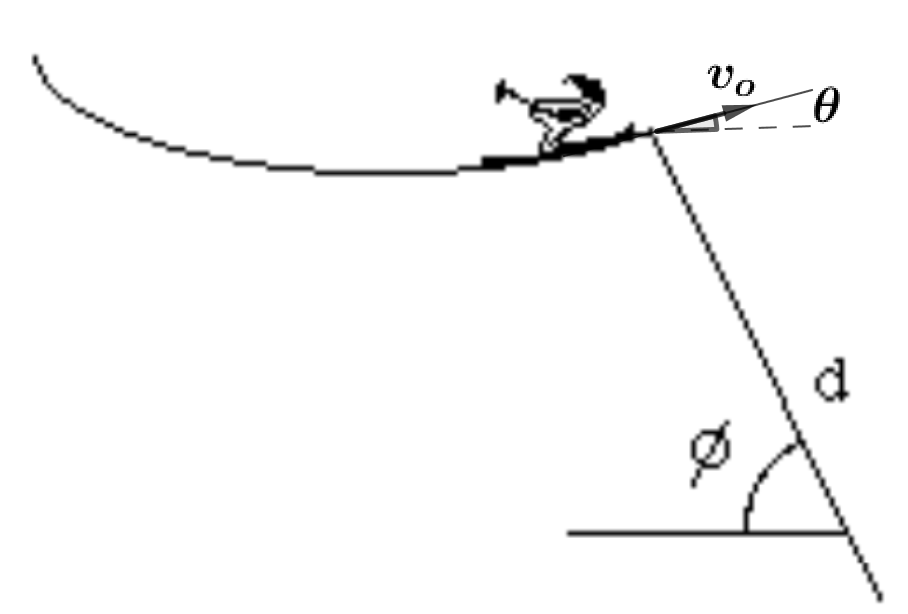
\includegraphics[width=.5\textwidth]{imagenes/imagenes02/T02IM37.png}
		\end{figure}
El problema es similar al anterior pero para $\phi>90^o$. 
Llamando al ángulo del plano inclinado $-\phi$, podremos usar las fórmulas anteriores.

\begin{figure}[H]
		\centering
		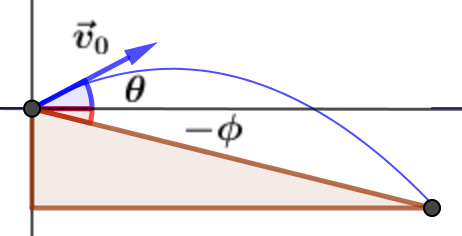
\includegraphics[width=.3\textwidth]{imagenes/imagenes02/T02IM38.png}
		\end{figure}

\end{multicols}


\vspace{-3mm}\begin{figure}[H]
		\centering
		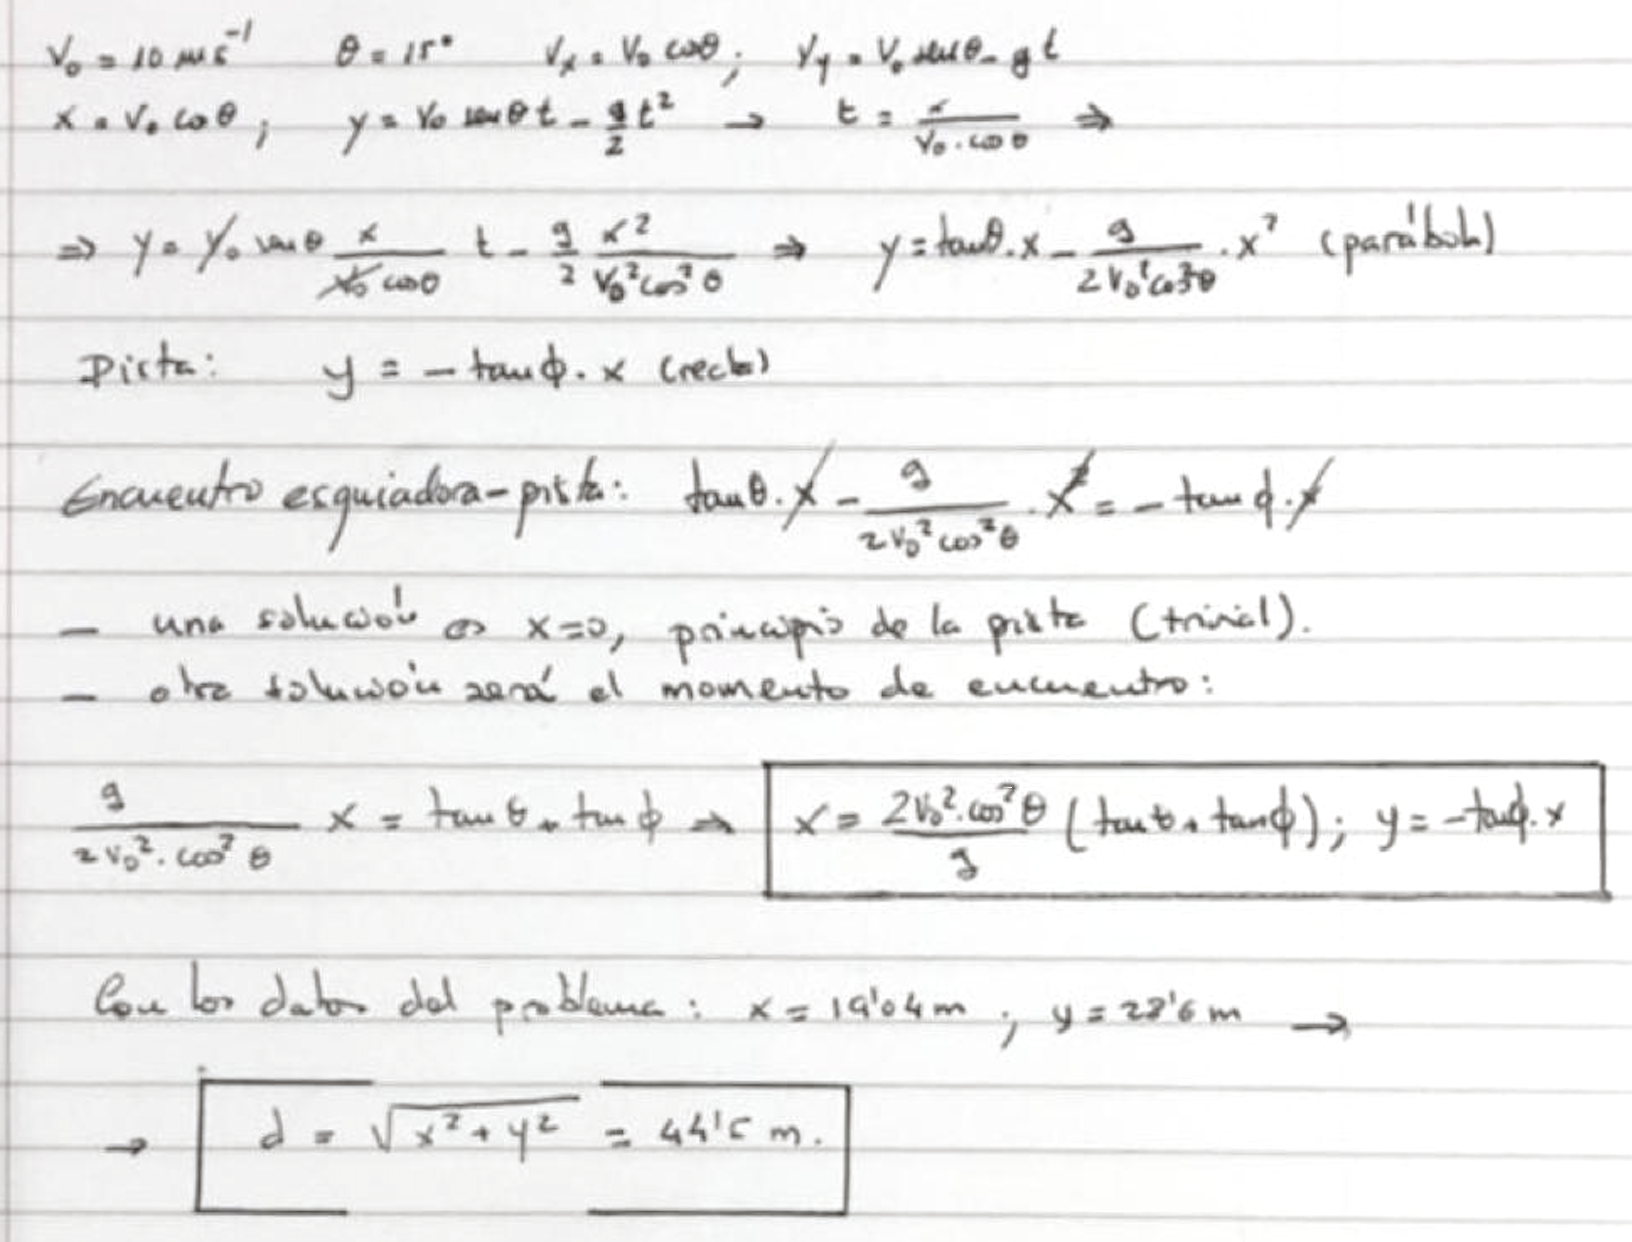
\includegraphics[width=1\textwidth]{imagenes/imagenes02/T02IM40.png}
		\end{figure}
		
	
		
\vspace{-3mm}\textbf{Análisis de casos límites:} 

Si en la expresión encontrada, $x=\dfrac{2v_0 \cos^2 \theta}{g}(\tan \theta+\tan \phi)$, hacemos $\phi=0$, se obtiene $x=\dfrac{v_0^2}{g} \sin 2\theta=x_{max}$, alcance máximo de un proyectil en superficie horizontal.



\begin{myblock}{Cinemática}
	
\begin{small}
El nacimiento de la cinemática moderna tiene lugar con la alocución de Pierre Varignon el 20 de enero de 1700, ante la Academia Real de las Ciencias de París. Fue allí cuando definió la noción de aceleración y mostró cómo es posible deducirla de la velocidad instantánea utilizando un simple procedimiento de cálculo diferencial.

\vspace{2mm} En la segunda mitad del siglo XVIII se produjeron más contribuciones por Jean Le Rond d'Alembert, Leonhard Euler y André-Marie Ampère y continuaron con el enunciado de la ley fundamental del centro instantáneo de rotación en el movimiento plano, de Daniel Bernoulli.

\vspace{2mm} El vocablo cinemática fue creado por André-Marie Ampère, quien delimitó el contenido de esta disciplina y aclaró su posición dentro del campo de la mecánica. Desde entonces, la cinemática ha continuado su desarrollo hasta adquirir una estructura propia.

\vspace{2mm} Con la teoría de la relatividad especial de Albert Einstein en 1905, se inició una nueva etapa, la cinemática relativista, donde el tiempo y el espacio no son absolutos, y sí lo es la velocidad de la luz.

\vspace{2mm} Los elementos básicos de la cinemática son el espacio, el tiempo y un móvil.

\vspace{2mm} La cinemática trata del estudio del movimiento de los cuerpos en general y, en particular, el caso simplificado del movimiento de un punto material, mas no estudia por qué se mueven los cuerpos sino que se limita a describir sus trayectorias y modo de reorientarse en su avance.

\vspace{2mm} El movimiento trazado por una partícula lo mide un observador respecto a un sistema de referencia. Desde el punto de vista matemático, la cinemática expresa cómo varían las coordenadas de posición de la partícula (o partículas) en función del tiempo. La función matemática que describe la trayectoria recorrida por el cuerpo (o partícula) depende de la velocidad (la rapidez con la que cambia de posición un móvil) y de la aceleración (variación de la velocidad respecto del tiempo).

\vspace{2mm} \textbf{Tipos de movimientos}:

--- Si la aceleración es nula, da lugar a un movimiento rectilíneo uniforme y la velocidad permanece constante a lo largo del tiempo.

--- Si la aceleración es constante con igual dirección que la velocidad, da lugar al movimiento rectilíneo uniformemente acelerado y la velocidad variará a lo largo del tiempo.

--- Si la aceleración es constante con dirección perpendicular a la velocidad, da lugar al movimiento circular uniforme, donde el módulo de la velocidad es constante, cambiando su dirección con el tiempo.

--- Cuando la aceleración es constante y está en el mismo plano que la velocidad y la trayectoria, tiene lugar el movimiento parabólico, donde la componente de la velocidad en la dirección de la aceleración se comporta como un movimiento rectilíneo uniformemente acelerado, y la componente perpendicular se comporta como un movimiento rectilíneo uniforme, y se genera una trayectoria parabólica al componer ambas.

--- Cuando la aceleración es constante pero no está en el mismo plano que la velocidad y la trayectoria, se observa el efecto de Coriolis.

--- En el movimiento armónico simple se tiene un movimiento periódico de vaivén, como el del péndulo, en el cual un cuerpo oscila a un lado y a otro desde la posición de equilibrio en una dirección determinada y en intervalos iguales de tiempo. La aceleración y la velocidad son funciones, en este caso, sinusoidales del tiempo.


\vspace{2mm} Un movimiento interesante es el de una peonza, que al girar puede tener un movimiento de precesión y de nutación. Cuando un cuerpo posee varios movimientos simultáneamente, como por ejemplo uno de traslación y otro de rotación, se puede estudiar cada uno por separado en el sistema de referencia que sea apropiado para cada uno, y luego, superponer los movimientos.

\vspace{2mm} \textbf{Movimiento sobre la Tierra}:

\vspace{2mm} Supongamos que un cañón situado en el ecuador lanza un proyectil hacia el norte a lo largo de un meridiano. Un observador situado al norte sobre el meridiano observa que el proyectil cae al este de lo predicho, desviándose a la derecha de la trayectoria. De forma análoga, si el proyectil se hubiera disparado a lo largo del meridiano hacia el sur, el proyectil también se habría desviado hacia el este, en este caso hacia la izquierda de la trayectoria seguida. La explicación de esta «desviación», provocada por el Efecto Coriolis, es debida a la rotación de la Tierra. El proyectil tiene una velocidad con tres componentes: las dos que afectan al tiro parabólico, hacia el norte (o el sur) y hacia arriba, respectivamente, más una tercera componente perpendicular a las anteriores debida a que el proyectil, antes de salir del cañón, tiene una velocidad igual a la velocidad de rotación de la Tierra en el ecuador. Esta última componente de velocidad es la causante de la desviación observada pues si bien la velocidad angular de rotación de la Tierra es constante sobre toda su superficie, no lo es la velocidad lineal de rotación, la cual es máxima en el ecuador y nula en el centro de los polos. Así, el proyectil conforme avanza hacia el norte (o el sur), se mueve más rápido hacia el este que la superficie de la Tierra, por lo que se observa la desviación mencionada. Lógicamente, si la Tierra no estuviese rotando sobre sí misma, no se daría esta desviación.

\vspace{2mm} Otro caso interesante de movimiento sobre la Tierra es el del péndulo de Foucault. El plano de oscilación del péndulo no permanece fijo, sino que lo observamos girar, girando en sentido horario en el hemisferio norte y en sentido antihorario en el hemisferio sur. Si el péndulo se pone a oscilar en el ecuador, el plano de oscilación no cambia. En cambio, en los polos, el giro del plano de oscilación toma un día. Para latitudes intermedias toma valores mayores, dependiendo de la latitud. La explicación de tal giro se basa en los mismos principios hechos anteriormente para el proyectil de artillería \end{small}\normalsize{.}
\end{myblock}




\chapter{Dinámica de la partícula. Campos de fuerza}	
\chaptermark{Dinámica de la partícula}

La dinámica es una parte de la mecánica en que, dadas unas condiciones, se estudia qué movimiento se va a producir.

Consideraciones: En mecánica clásica el \emph{espacio} es como un gran cajón donde está todo el universo físico. El \emph{tiempo} es absoluto: dados dos fenómenos, todos los relojes de todos los posibles observadores medirán lo mismo.

\rule{150pt}{0.4pt} 

Los fenómenos mecánicos se describen mediante sistemas de referencia basados en los conceptos de espacio y tiempo. Por su importancia conviene enunciar los postulados que asume la mecánica clásica para estos conceptos. 

El \emph{espacio}, y por tanto su métrica, tiene las propiedades siguientes. 
\begin{itemize}
\vspace{-2mm}\item Independencia de los objetos en él inmersos. (La métrica del espacio no se ve afectada por los mismos.) 
\vspace{-2mm}\item Constancia a lo largo del tiempo. 
\vspace{-2mm}\item \textbf{Homogeneidad: es igual en todos los puntos}, no existiendo puntos privilegiados. 
\vspace{-2mm}\item \textbf{Isotropía: es igual en todas las direcciones}, no existiendo direcciones privilegiadas. 
\end{itemize}
El espacio se caracteriza por una métrica euclídea:
 
$d(\;(x_1,y_1,z_1)\;(x_2,y_2,z_2)\;)=\sqrt{(x_2-x_1)^2+(y_2-y_1)^2+(z_2-z_1)^2}$ 

El \emph{tiempo} se caracteriza a su vez por las siguientes propiedades. 
\begin{itemize}
\vspace{-2mm}\item \textbf{Homogeneidad}, al no existir instantes privilegiados. 
\vspace{-2mm}\item Fluye constantemente en un sentido, por lo que no se puede retroceder ni volver al pasado. Asimismo, los fenómenos futuros no pueden condicionar los presentes. \textbf{No} se cumple por tanto la \textbf{isotropía}, existiendo un único sentido en el que puede discurrir el tiempo. 
\vspace{-2mm}\item \textbf{Simultaneidad absoluta}: Los fenómenos considerados simultáneos para dos observadores en sendos sistemas de referencia lo son asimismo para cualquier otro observador ligado a cualquier otro sistema de referencia. 
\end{itemize}

\setlength{\parindent}{0pt} %Aparecía sangrado en 1a linea, esto lo evita
En mecánica clásica, el tiempo se considera una variable de naturaleza distinta de las variables espaciales y la métrica euclídea no está influenciada por él. 

Algunos de estos postulados básicos no son aceptados por la mecánica relativista. La teoría de la relatividad restringida establece una referencia en cuatro dimensiones espacio-tiempo. La teoría de la relatividad general establece un espacio curvado, con métrica riemanniana no euclídea, debido a la presencia de masas que condicionan dicha métrica. De esta forma el espacio no sería independiente de los objetos en él inmersos 

\rule{150pt}{0.4pt} 

Una vía para abordar los problemas de la mecánica es averiguar las `causas del movimiento': ``el \emph{movimiento} es debido a la \emph{interacción} que se ejerce entre las diversas partes o cuerpos de universo''.


\section{Leyes del movimiento. Newton (3)}

\begin{cita}
``Si he visto más lejos que los demás es porque estoy sentado sobre los hombros de gigantes'' (Isaac Newton).
\end{cita} 

\vspace{-13mm}\scriptsize{Isaac Newton (1643-1727) escribió esa frase en una carta a Robert Hooke en la que hacía mención a sus predecesores Copérnico, Galileo y Kepler}\normalsize{.}

\vspace{4mm}A las entidades responsables de que los cuerpos varíen su posición en el espacio absoluto newtoniano les llamaremos \emph{interacciones} o \emph{fuerzas.}

En el siglo $XVIII$, Newton postula las tres leyes de la mecánica clásica.

\vspace{3mm}
\begin{miparrafo}

\textbf{1. } \emph{``Todo cuerpo permanece en reposo o en movimiento uniforme a menos que se obre sobre él alguna fuerza''.} Es la llamada \textsf{Ley de Inercia.}

\textbf{2. } \emph{``Todo cuerpo sobre el que actúa una fuerza se mueve de forma tal que la variación de su cantidad de movimiento por unidad de tiempo es igual a la fuerza''.} \textsf{Fuerza igual a masa por aceleración.}

\textbf{3. } \emph{``Cuando dos cuerpos ejercen entre sí fuerzas, éstas son de intensidades iguales y sentidos opuestos y están dirigidas a lo largo de la línea que une a los dos cuerpos considerados como partículas''.} 
\textsf{Ley de Acción y Reacción.}

\end{miparrafo}

En la primera ley se introduce la `fuerza' cualitativamente, en la segunda cuantitativamente.

Hemos introducido una nueva magnitud, la \emph{cantidad de movimiento}, 

\begin{equation}
\label{cant-mov}
\subrayado{\vec p=m\; \vec v} \qquad \qquad  \textcolor{gris}{[\vec p]=[\mathrm{MLT}^{-1}]\to \mathrm{kg\ m\ s}^{-1}}
\end{equation}

\begin{equation}
\label{Newton}
\subrayado{\vec F=\dv{\vec p}{t}} 	\qquad \qquad  \textcolor{gris}{[\vec F]=\dfrac{[\vec p]}{[t]}=[\mathrm{MLT}^{-2}]\to \mathrm{kg\ m\ s}^{-2}=\mathrm{N}}
\end{equation}


\emph{Primera hipótesis de la mecánica clásica:} La \emph{masa} es una característica especial de los cuerpos que interaccionan y no varía respecto al tiempo, es \emph{constante}.

\begin{equation}
\label{fma}
 \boldsymbol{ \vec F}=\dv{\vec p}{t}=\dv{(m\; \vec v)}{t}=m\; \dv{\vec v}{t}=\boldsymbol{ m\; \vec a}
\end{equation}


Supongamos dos cuerpos interactuando: $\vec F_1=m_1\ \vec a_1$ y  $\vec F_2=m_2\ \vec a_2$. Supongamos que forman un sistema aislado en el espacio, es decir, el resto de cuerpos del universo ejercen sobre ellos una interacción despreciable.

Por el tercer postulado (ley) de Newton, tenemos: $\vec F_1=-\vec F_2$, es decir, $m_1\; \vec a_1=-m_2\;\vec a_2\;:$
$$\displaystyle \dfrac {m_2}{m_1}=\dfrac {a_1}{a_2}$$
Tomamos un cuerpo cualquiera del universo de masa $m_1$ que no conocemos y, arbitrariamente, le damos el valor de `masa unidad', con lo que para otro cuerpo, $\displaystyle m_2=\dfrac {a_1}{a_2}\; m_1$ y así introducimos el concepto de masa.

\begin{figure}[]
		\centering
		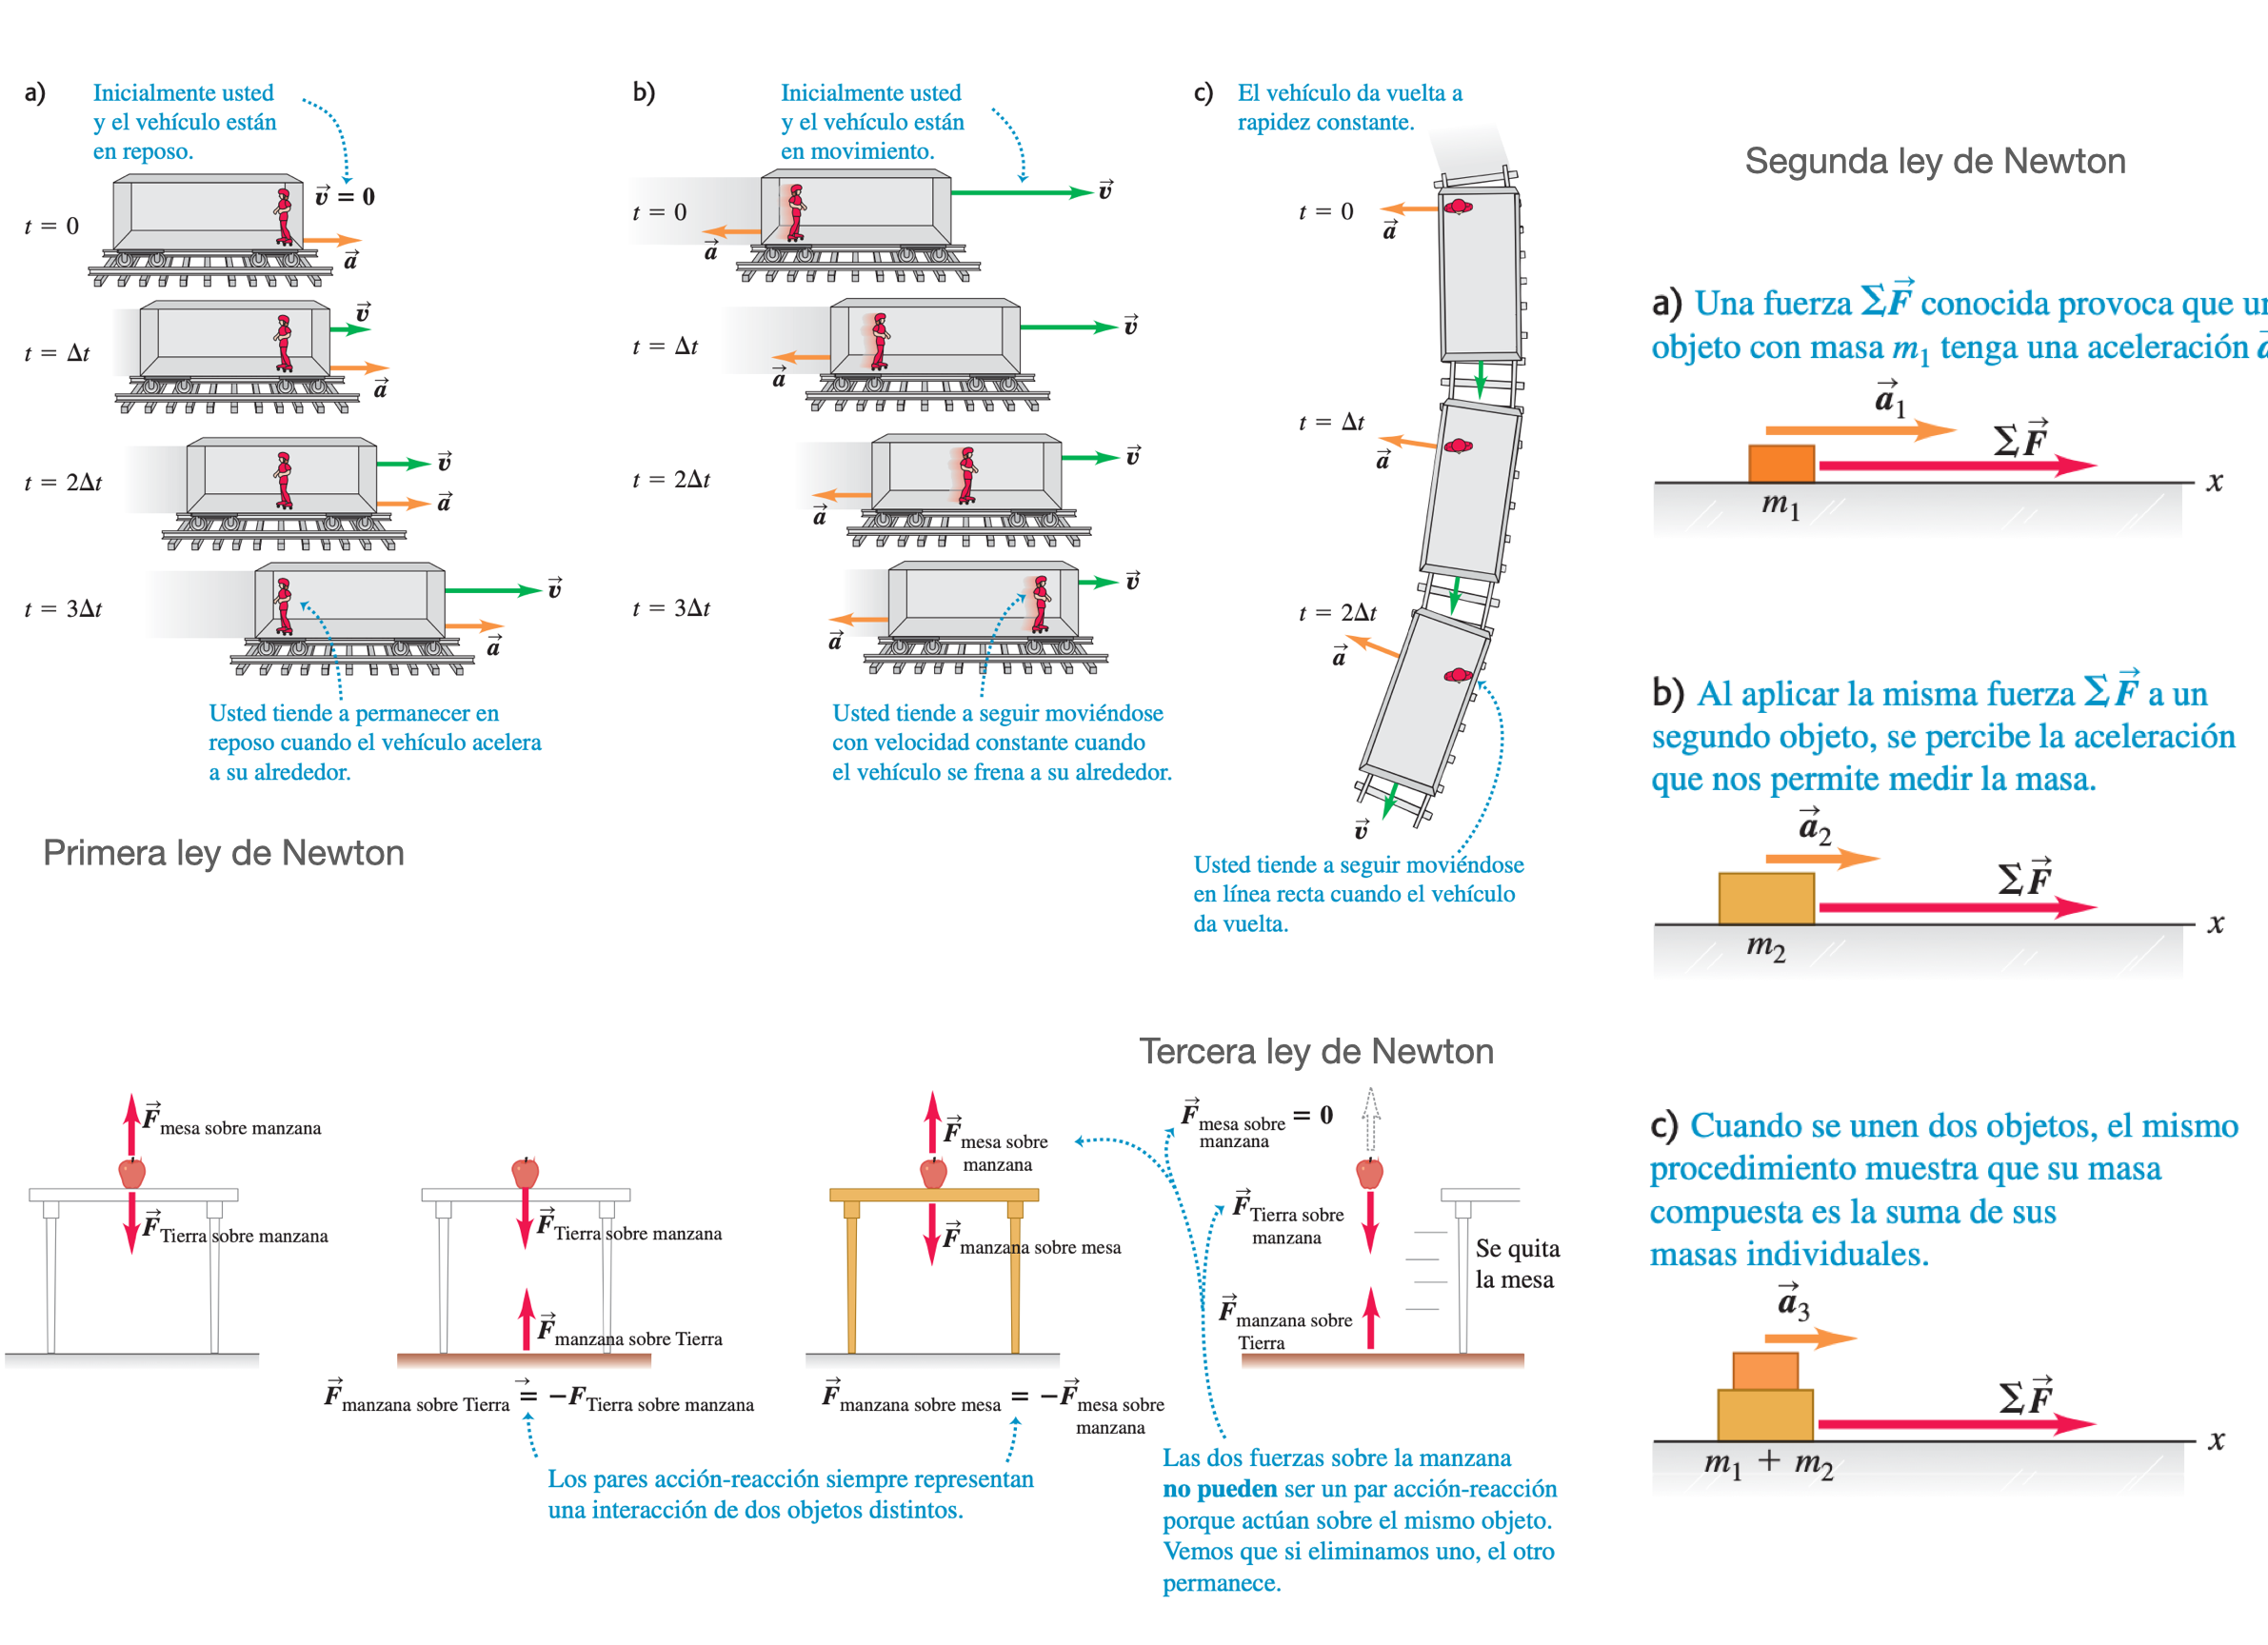
\includegraphics[width=1\textwidth]{imagenes/imagenes03/T03IM02.png}
		\end{figure}

Por extensión de la ley de Newton, tenemos: $Peso=m_G\; a \;\; \wedge\;\; F=m_I\; a$, donde $g$ es la aceleración de la gravedad, $m_G$ la masa gravitatoria y $m_I$ la masa inercial ($m$ es la constante de proporcionalidad entre $\vec F$ y $\vec a$).

\textbf{Igualdad entre masa inercial y masa gravitatoria: Otro enigma sin resolver.}

Fijémonos despacio en las fórmulas de Newton. Cuando aplicas una fuerza $\vec F$ a un cuerpo con cierta masa $m_I$, éste se acelera con cierta aceleración $\vec a\; / \vec F=m_I\; \vec a$. Hemos llamado $m_I$ a la masa para recordar que estamos hablando de la ``resistencia’’ que opone esa masa a acelerarse (su inercia; de ahí el subíndice `I’).

Pero sabemos que el mismo cuerpo ejerce una atracción gravitatoria sobre todos los demás. Por ejemplo, si pesamos ese cuerpo, lo que estamos haciendo es medir la fuerza gravitatoria entre él y la Tierra, que será $F=G \dfrac{M_T\; m_G}{{R_T}^2}$, donde $M_T$ es la masa de la Tierra, $R_T$ su radio y $m_G$ es la masa del cuerpo en cuestión (que ahora llamamos $m_G$ para remarcar que nos referimos a la masa que produce la atracción gravitatoria). 

Si ahora imaginamos un experimento fácil en el que queremos medir la aceleración que produce la fuerza de la gravedad, no tenemos más que igualar las dos fórmulas:
$$m_I\;a= G \dfrac{M_T\; m_G}{{R_T}^2} \to a= \dfrac{m_G}{m_I}\;G\dfrac{M_R}{{R_T}^2}$$
Midiendo la aceleración $a$ en muchos experimentos diferentes, con objetos de masas diferentes, se ve que es siempre igual (y por eso se le llama $g$, la aceleración de la gravedad en la superficie terrestre) y, por tanto,  $\boldsymbol {m_G/m_I=1}$, o sea encontramos que la masa gravitatoria es igual a la masa inercial en cualquier cuerpo. (Experimentos de EOTVOS-1891 y DICKE-1950)

La pregunta que ya se hizo Newton es: ?`por qué tienen que ser necesariamente iguales $m_I$ y $m_G$? Son conceptualmente diferentes: $m_I$ representa cómo una cantidad de materia se opone a que la aceleren mientras que $m_G$ representa cómo atrae esa cantidad de materia a cualquier otra.

Como hemos dicho, experimentalmente se mide que ambas son iguales. Pero tenemos que recordar que la precisión de los aparatos con los que medimos en los experimentos científicos no es infinita. Por tanto, no podemos estar absolutamente seguros de que sean exactamente iguales, lo más que podemos decir es que son iguales hasta una precisión muy elevada (una parte en diez billones). O sea, en una masa de un kilo, $m_I$ y $m_G$ podrían ser diferentes en una milmillonésima de miligramo, no más. Hecha esta aclaración, podemos asegurar que la masa inercial y la masa gravitatoria son iguales hasta donde alcanza la precisión de nuestras medidas.

Einstein también pensó en este enigma. No lo resolvió (es decir, no encontró una teoría que demostrara que las masas gravitacional e inercial tienen que ser iguales) pero, como estaba convencido de que dicha igualdad no era por casualidad, supuso que era un principio fundamental del universo (como el del límite de la velocidad de la luz) y lo llamo \textbf{\emph{``principio de equivalencia''}}. Este principio es fundamental en su teoría de la gravitación, la teoría general de la relatividad.

		
\section[Fuerzas de rozamiento. Rozamientos estático y dinámico]{Fuerzas de rozamiento. Rozamientos estático y dinámico \sectionmark{Fuerzas de rozamiento}}
\sectionmark{Fuerzas de rozamiento}

Al arrojar un cuerpo sobre una mesa observamos que	éste se desliza por ella y, al cabo de un tiempo	 $t$, se para. \emph{Las fuerzas de rozamiento son aquellas que actúan siempre oponiéndose al sentido del movimiento de los cuerpos.}

\begin{multicols}{2}
En un momento determinado en que hay un determinado número de pesas en la balanza, el cuerpo se pone en movimiento: $\ \boldsymbol{F\ge F_{RE}}$.

La fuerza de rozamiento estático depende de la naturaleza de los cuerpos que rozan.

La relación entre la fuerza máxima de rozamiento estático y la fuerza normal $(N)$ se llama \emph{coeficiente de rozamiento estático:} $\ F_{RE}=\mu_{RE}\ N$

En general,

$\vec F_{tot}=\vec F-\vec F_{RE}=m\ \vec a$

\begin{figure}[H]
		\centering
		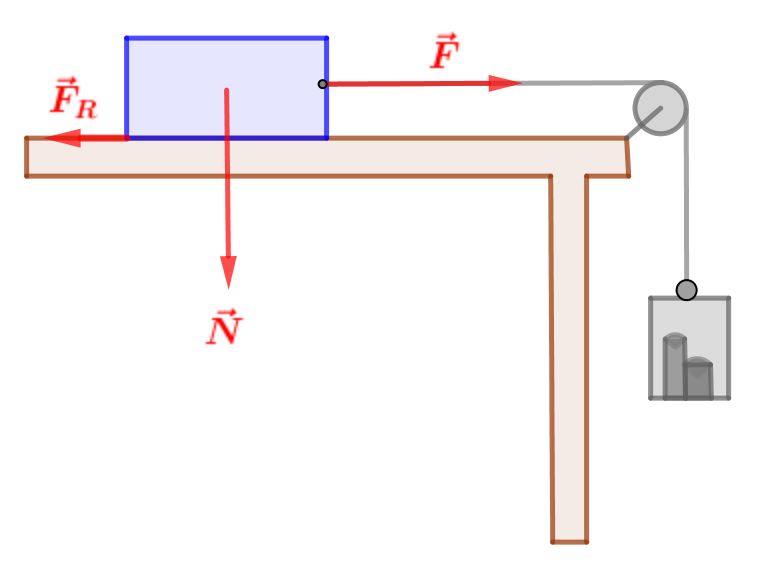
\includegraphics[width=.4\textwidth]{imagenes/imagenes03/T03IM48.png}
		\end{figure}		
\end{multicols}		
		
\textbf{Plano inclinado}
		
\begin{multicols}{2}
A medida que aumenta $\alpha$, aumenta la componente tangencial del peso, $\vec F_T$. En el momento en que el cuerpo empiece a deslizar,

\begin{figure}[H]
		\centering
		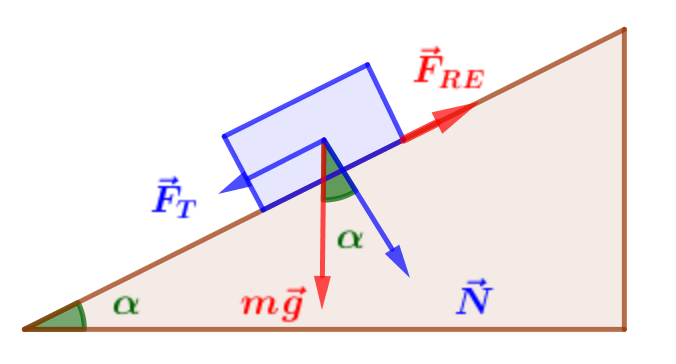
\includegraphics[width=.35\textwidth]{imagenes/imagenes03/T03IM49.png}
		\end{figure}		
\end{multicols}			
		
$F_T=F_{RE}=\mu_{RE}\vec N \quad \to \quad \mu_E=\dfrac {m g \sin \alpha}{m g \cos \alpha}=\tan \alpha$

El coeficiente de rozamiento estático se puede encontrar como la tangente del ángulo mínimo para el que el cuerpo empieza a deslizar por el plano inclinado.

Experimentalmente se comprueba que, una vez empieza el cuerpo a moverse, la fuerza de mantenimiento puede ser menor que $F_{RE}$. Se suele hablar de \emph{rozamiento dinámico.}

$F_{RE}=\mu_{RE}\ N; \quad F_{RD}=\mu_{RD}\ N \le F_{RE} \Rightarrow \boldsymbol{\mu_{RD} \le \mu_{RE}}$		
		
$F_{RD}$ es la fuerza que hay que aplicar para mantener el cuerpo en movimiento.			



\begin{figure}[H]
		\centering
		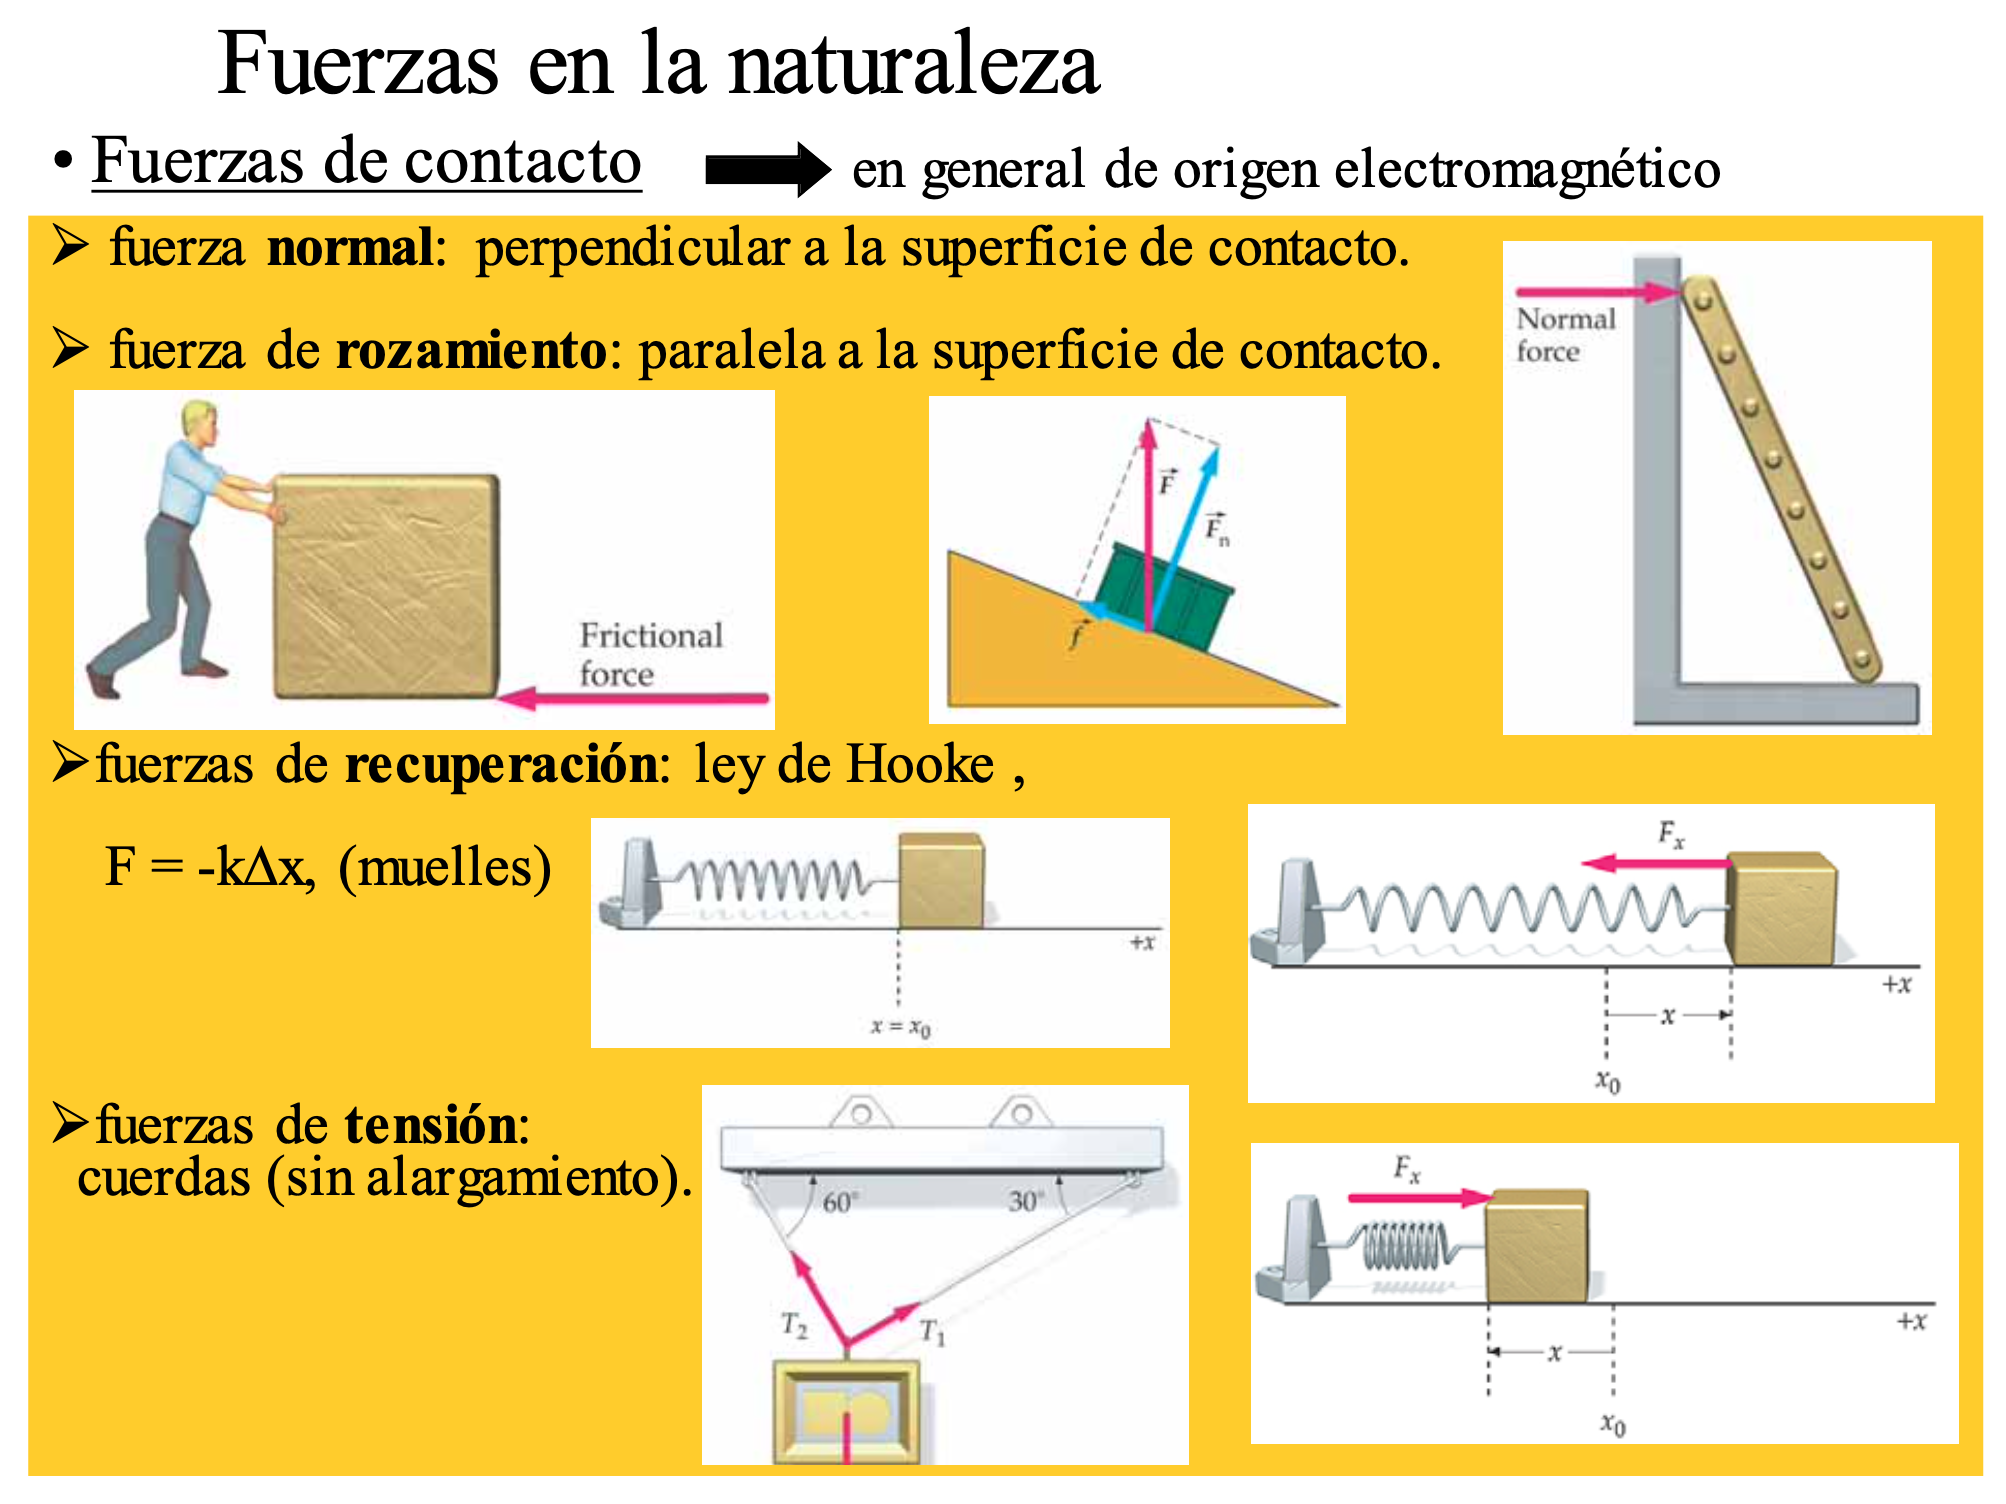
\includegraphics[width=.9\textwidth]{imagenes/imagenes03/T03IM06.png}
		\end{figure}
\begin{figure}[H]
		\centering
		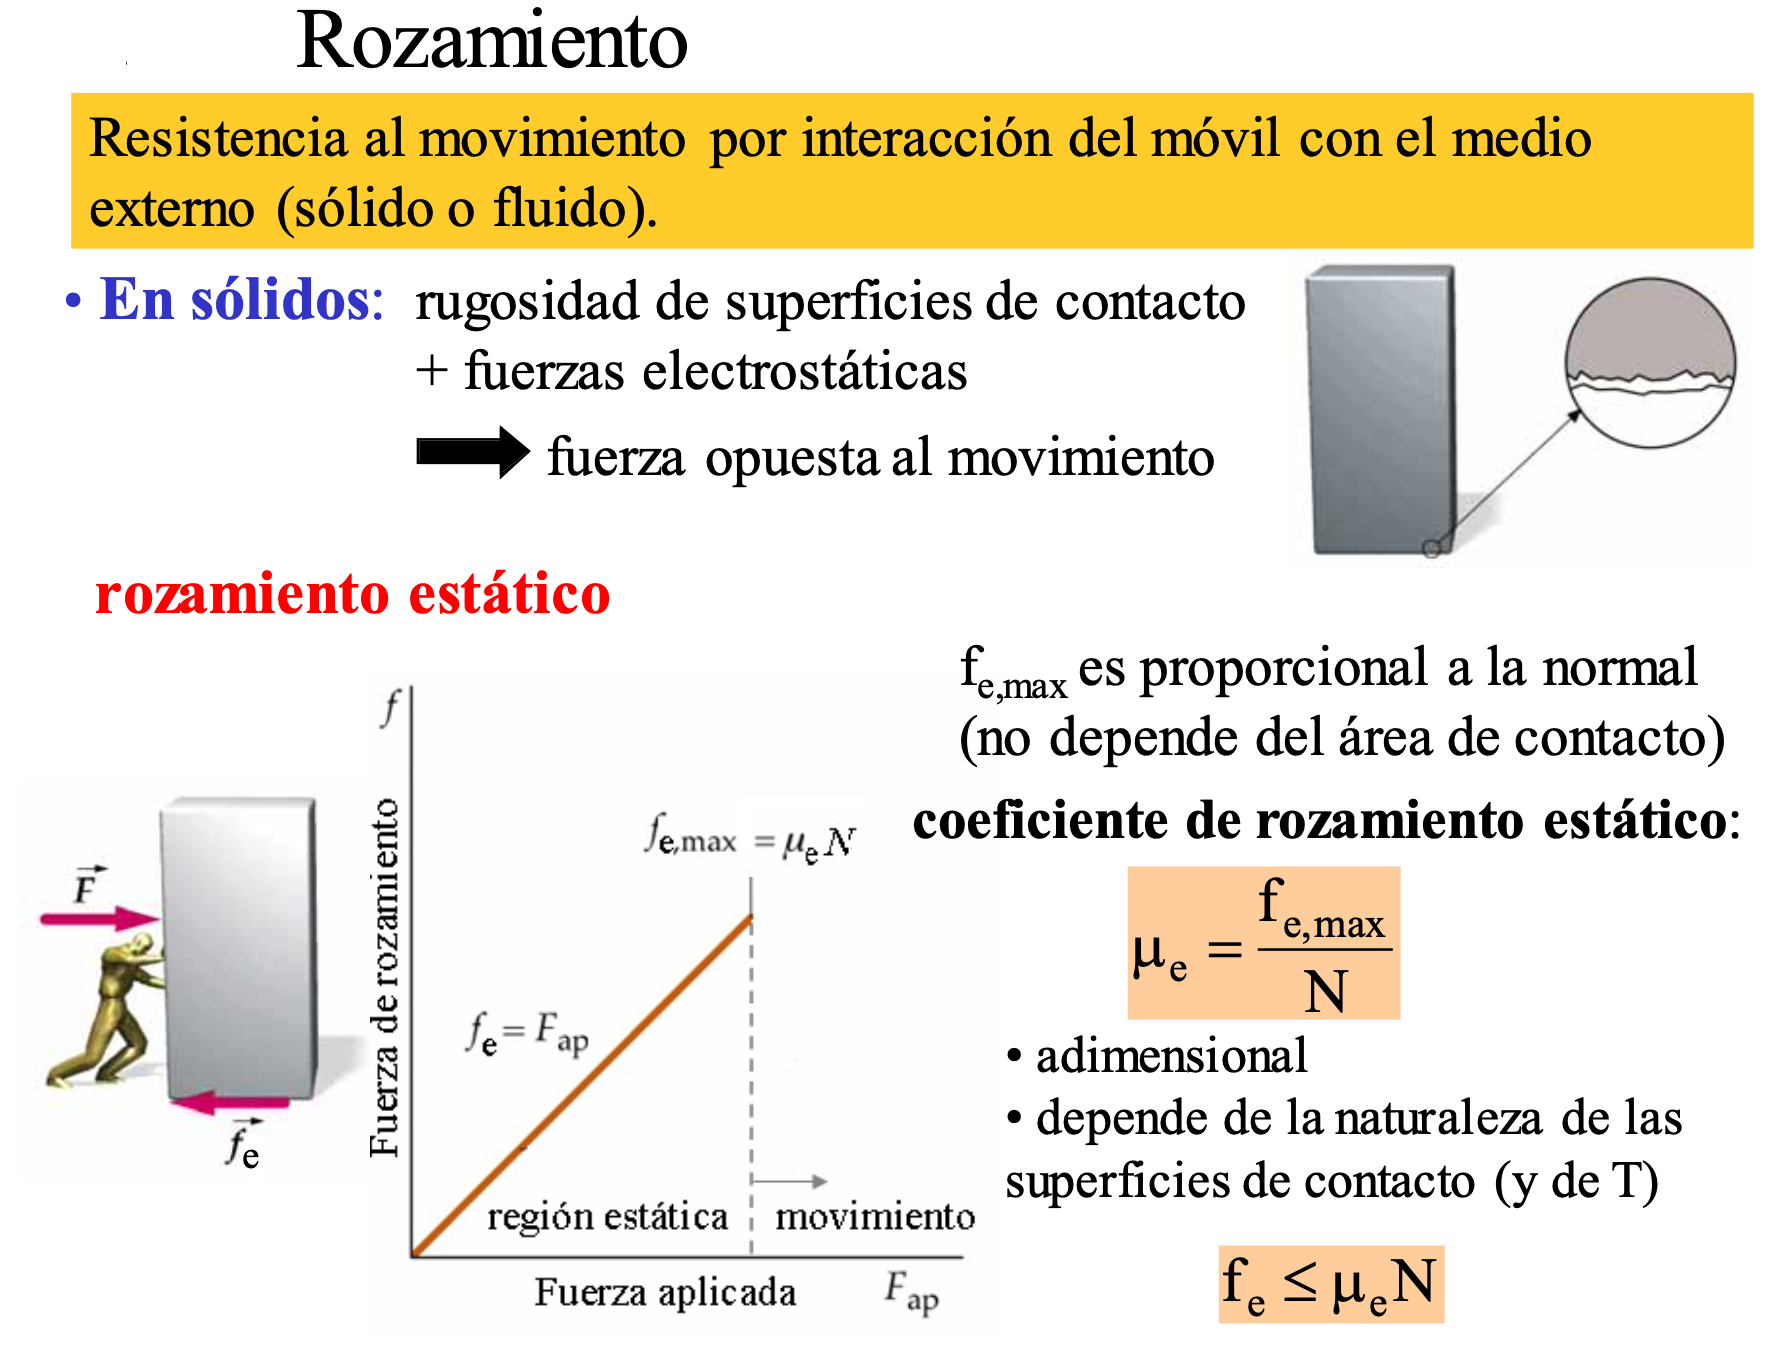
\includegraphics[width=1\textwidth]{imagenes/imagenes03/T03IM07.png}
		\end{figure}
\begin{figure}[H]
		\centering
		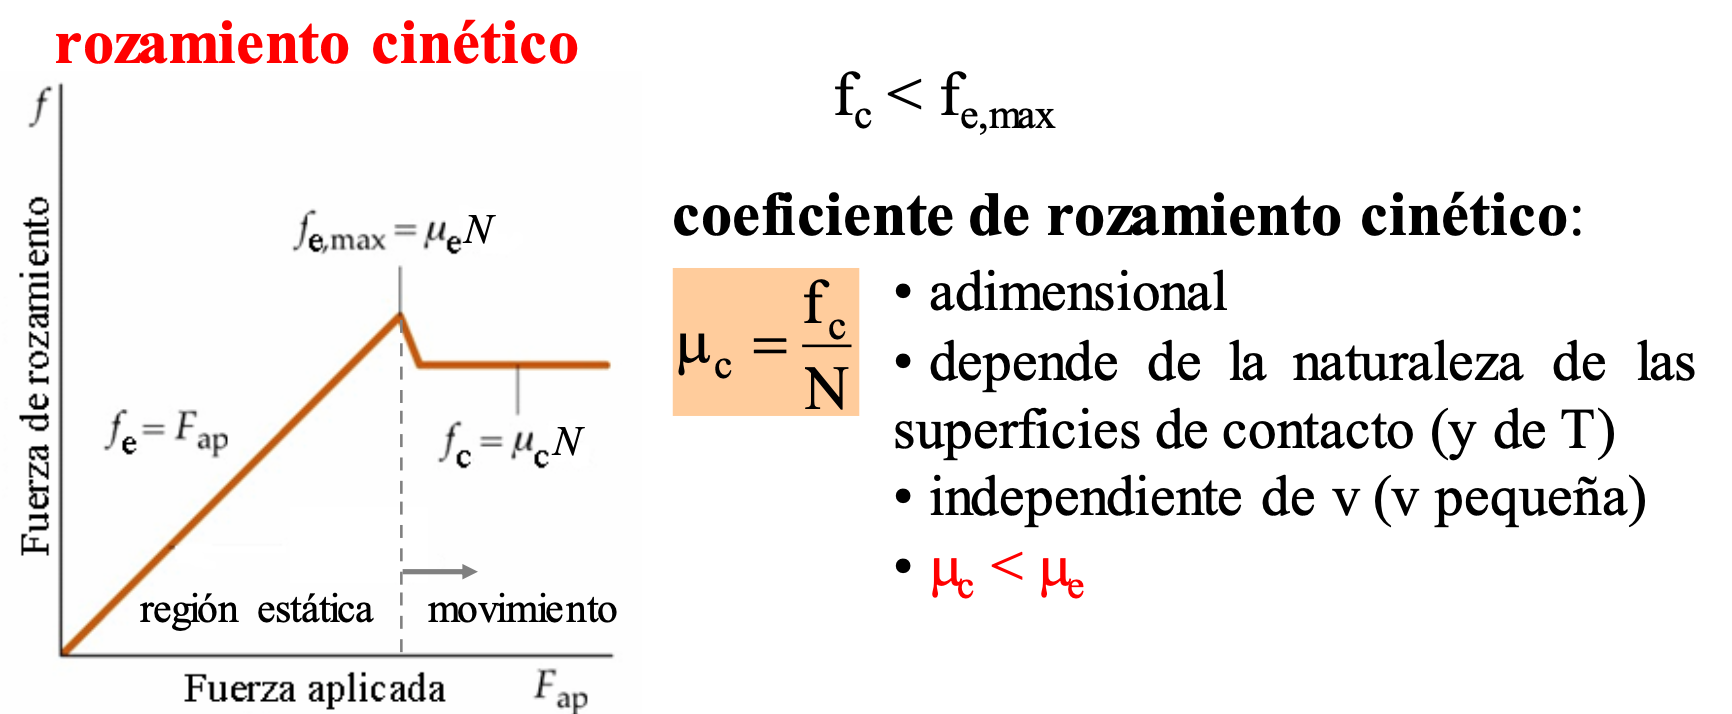
\includegraphics[width=1\textwidth]{imagenes/imagenes03/T03IM08.png}
		\end{figure}		

\newpage %*****************************************************

\begin{figure}[H]
		\centering
		\includegraphics[width=.95\textwidth]{imagenes/imagenes02/T02IM31.png}
		\end{figure}

\begin{figure}[H]
		\centering
		\includegraphics[width=.95\textwidth]{imagenes/imagenes02/T02IM32.png}
		\end{figure}

			
\section{Trabajo de una fuerza}

\begin{multicols}{2}
Por definición, diremos que el \emph{trabajo elemental} $\boldsymbol{\dd W}$ que realiza un cuerpo $m$  al pasar de una posición $\vec r$ a otra infinitamente próxima $\vec r+ \dd \vec r$ es: 

\begin{equation}
\label{def-trabajo}
\subrayado{\dd W= \vec F \cdot \dd \vec r}
\end{equation}

$ (\ \boldsymbol{\cdot} \ \equiv \text{producto\; escalar})$

\begin{figure}[H]
		\centering
		\includegraphics[width=.45\textwidth]{imagenes/imagenes03/T03IM01.png}
		\end{figure}
\end{multicols} 



El trabajo total para ir de un punto $A$ hasta otro $B$ es:

\begin{equation}
\label{trabajo}
W=\int_A^B\vec F \cdot \dd \vec r	
\end{equation}

En el caso particular en que $\vec F=\overrightarrow{cte}$, 
$W=\vec F \cdot \int_A^B \dd \vec r=\vec F\cdot (\vec r_B-\vec r_A)=\vec F \cdot \Delta \vec r$

\begin{multicols}{2}
Si además el desplazamiento es en línea recta, el trabajo es el producto del desplazamiento por la componente tangencial de la fuerza.º

\vspace{3mm} %**********************************************
$W=\vec F\cdot \Delta \vec r=F\; \Delta r\; 	\cos \theta= (F\; \cos \theta)\; \Delta r= F_T \;\Delta r$

\vspace{3mm} %**********************************************
Dimensionalmente, $[W]=[\mathrm{FL}]=[\mathrm{ML}^2\mathrm{T}^{-2}]$. Su unidad es el Joule, $\mathrm{J}=\mathrm{N} \cdot \mathrm{m}$. El trabajo es un escalar.
\begin{figure}[H]
		\centering
		\includegraphics[width=.4\textwidth]{imagenes/imagenes03/T03IM03.png}
		\end{figure}	
\end{multicols}





\begin{figure}[H]
		\centering
		\includegraphics[width=.8\textwidth]{imagenes/imagenes03/T03IM04.png}
		\end{figure}

\vspace{-4mm}\noindent \small{\textcolor{gris}{$dW=\vec F \cdot \dd \vec r:\begin{cases}  \vec r=x\vec i +y \vec j \\  \vec F=\vec F(x,y) \end{cases} \hspace{-2mm}\to  y=y(x) \Rightarrow  \begin{cases} \dd \vec r=\dd \vec r(x,y(x)) \\ \vec F=\vec F(x) \end{cases} \hspace{-2mm} \dd W= \dd W(x)$}\normalsize{.}}

\begin{figure}[H]
		\centering
		\includegraphics[width=.8\textwidth]{imagenes/imagenes03/T03IM13.png}
		\end{figure}

\section{Concepto de energía}

\normalsize{Un} \emph{fenómeno físico} es una variación en las condiciones que se dan en un sistema físico.

Podemos distinguir entre dos tipos de fueras:

\vspace{-2mm}\begin{itemize}
\vspace{-2mm}\item \emph{fuerzas exteriores} que actúan sobre un sistema físico y pueden modificarlo (al soltar un objeto de la mano cae al suelo por efecto de la fuerza externa de la gravedad que actúa sobre él).
\vspace{-2mm}\item \emph{fuerzas interiores} que actúan sobre un sistema físico y pueden modificarlo 	(un átomo de carbono 14 se convierte en nitrógeno 14 emitiendo un electrón --- desintegración $\beta:\; ^{14}_6C \to ^{14}_7N+^0_{-1}e$---).
\end{itemize}

Cuando se modifica el estado de un sistema físico se atribuye a las fuerzas y producen movimientos. \emph{Las fuerzas en movimiento son trabajo}, luego los sistemas físicos tienen \emph{energía}. 

Llamamos \emph{\colorbox{LightYellow}{energía}} a \emph{la \colorbox{LightYellow}{capacidad} que tienen los sistemas físicos para \colorbox{LightYellow}{realizar un trabajo}.}, es una propiedad que tienen los cuerpos y se va a medir con las mismas unidades y dimensiones que el trabajo. La energía es un escalar.

Podemos distinguir entre tres tipos de energia:

\begin{miparrafo}

\textbf{---} \emph{Energía cinética}: capacidad para realizar trabajo que tiene un cuerpo debido a su estado de movimiento (proyectil estrellado contra una pared).

\textbf{---} \emph{Energía potencial}: capacidad para realizar trabajo que tiene un cuerpo debido a la posición que ocupa en el espacio  (objeto que cae desde una determinada altura)

\textbf{---} \emph{Energía interna}: capacidad para realizar trabajo que tiene un cuerpo debido a su propia estructura interna (petardo de pólvora que explota por la temperatura).

\end{miparrafo}

La cantidad total de energía que tiene un sistema físico no es medible por la mecánica clásica, solo podemos medir variaciones de energía.


\section[Energía cinética. Teorema de las fuerzas vivas]{Energía cinética. Teorema de las fuerzas vivas\sectionmark{Energía cinética}}
\sectionmark{Energía cinética}

Definimos la energía cinética $\;\mathcal E_c\;$ como el trabajo necesario para que un cuerpo de masa $m$ cambie su celeridad (módulo de la velocidad) desde $v_0$ a $v_f$.
$$\subrayado{\Delta \mathcal E_c=W}=\displaystyle \int_1^2 \vec F \cdot \dd \vec r$$
desde el estado $1\to v_o$ hasta el estado $2\to v_f$. Por la segunda de Newton:

$\Delta \mathcal E_c=\displaystyle \int_1^2 \dv{\vec p}{t}\cdot \dd \vec r =\int_1^2 \dd \vec p \cdot \dv{\vec r}{t}
= \int_1^2 \vec v \cdot \dd \vec p=\dfrac 1 m\int_1^2 m\;\vec v \cdot \dd \vec p=
\dfrac 1 m \int_1^2 \vec p\cdot \dd \vec p$

$p^2=\vec p\cdot \vec p \to $ tomando diferenciales: $\cancel{2\;} p\;\dd  p= \cancel{2}\; \vec p \cdot \dd \vec p \to\;\; p\;\dd p=\vec p \cdot \dd \vec p$

$\Delta \mathcal E_c=\displaystyle \int_1^2 \dfrac 1 m \;p\; dp=\int_1^2 v\;\dd p =\int_1^2\; v  \dd (mv)=\int_1^2 m (m\dd v + v\dd m)$

\begin{equation}
	\Delta \mathcal E_c=\displaystyle\int_1^2 m\ v\;\dd v + \int_1^2 v^2 \ \dd m
\end{equation}

Ecuación que da la expresión exacta de la energía cinética entre deos estados $1$ y $2$


En el caso especial de partículas o cuerpos rígido, $ m=cte  \to  \Delta \mathcal E_c= \displaystyle m\ \int_1^2 v \ \dd v $:

\begin{equation}
\label{fuerzas-vivas}
\Delta \mathcal E_c= \frac 1 2 \ m \ v_2^2 - \frac 1 2 \ m \ v_1^2 = \mathcal E_{c_2}-\mathcal E_{c_1}
\end{equation}

Ecuación que recibe el nombre de \emph{\colorbox{LightYellow}{`Teorema de las fuerzas vivas'}.}
(Leibniz, en el $s.\ XVII$ llamó ``fuerza viva'' al producto $m \ v^2$).

\emph{El trabajo realizado por las fuerzas del campo al evolucionar el sistema dede un estado $1$ con $v_1$ a un estado $2$ con $v_2$ viene dado por la diferencia entre energías cinéticas ($\frac 1 2$ fuerza viva) entre el estado final $2$ y el estado inicial $1$.}


En el supuesto que:
\vspace{-2mm}\begin{itemize}
\vspace{-2mm}\item $v_1>v_2 \to \mathcal E_1 < \mathcal E_2 \to \Delta \mathcal E_c<0$ y el trabajo desarrollado se usa en frenar a la partícula.
\vspace{-2mm}\item $v_1<v_2 \to \mathcal E1 < \mathcal E_2 \to \Delta \mathcal E_c>0$ y el trabajo desarrollado se invierte en acelerar a la partícula.
\vspace{-2mm}\item $v_1=v_2 \to \mathcal E_1 = \mathcal E_2 \to \Delta \mathcal E_c=0$ y no se realiza trabajo. 	
\end{itemize}

\begin{figure}[H]
		\centering
		\includegraphics[width=1\textwidth]{imagenes/imagenes03/T03IM05.png}
		\end{figure}


\begin{multicols}{2}
	$W=\Delta \mathcal E_c==\frac 1 2 m v_f^2-\frac 1 2 m v_i^2$
	
	$\vec F=\vec N+\vec T$
	
	$\dd W _M=\vec N \cdot \dd \vec s=$
	
	$=(mg\sin \theta) \dd s \cos 90^o=0\to $ 
	
	$\to \quad W_N=0$
	\begin{figure}[H]
		\centering
		\includegraphics[width=.55\textwidth]{imagenes/imagenes03/T03IM47.png}
		\end{figure}
\end{multicols}
\vspace{-5mm}$\dd W_T= \vec T \cdot \dd \vec s=(mg \sin \theta) \dd s \cos 0^o \to W_T=mg\sin \theta \int_1^2 ds
=ms \sin \theta L=mgh$

$W=0+mgh=mgh=\mathcal E_c=\frac 1 2 m v_f^2$, parten del reposo: $v_i=0$

Luego $v_f=\sqrt{2gh}$. Ambas patinadoras llegan a meta con la misma velocidad y la menos experta gana la apuesta.

\textcolor{gris}{La patinadora que baja por la pista para expertos invierte menos tiempo en la bajada, pero esa no era la apuesta.}

\section{Potencia}

Se llama \emph{potencia} suministrada por una fuerza al trabajo por unidad de tiempo que realiza dicha fuerza. 

Potencia media: $\quad P=\dfrac{\Delta W}{\Delta t}$

Potencia instantánea: $\;\; P=\dfrac {\dd W}{\dd t}=\dfrac {\vec F \cdot \dd \vec r}{\dd t}=\vec F \cdot \vec v$

En general, para cualquier transferencia de energia, la potencia es: $\quad P=\dfrac{\dd E}{\dd t}$

Unidades: En el $SI:\;\; P\to  \ \mathrm{J s}^{-1} = \mathrm{W}$, wat. Una unidad de energía muy usada en ingeniería es el $\mathrm{kWh}=(10^3\ \mathrm{W})\ (3600\ \mathrm{s})=3.6\ 10^6 \ \mathrm{J}$.

\begin{ejem}
Un ascensor de $1000\ \mathrm{kg}$ soporta una carga máxima de $800 \ \mathrm{kg}$. Una fuerza de rozamiento constante de $400 \ \mathrm{N}$ retarda su movimiento hacia arriba haciendo que la subida sea a velocidad constante de $3 \ \mathrm{ms}^{-1}$. ?`Qué potencia suministra el motor?	
\end{ejem}
$F-F_R-(M+m)g=0 \to F=(1000+800)\ 9.8-4000=13640\ \mathrm{N}$

$P=F\ v=13640 \cdot 3 = 40920 \ \mathrm{W}= 40.920 \ \mathrm{KW}$

\textbf{Potencia y energía cinética.}

En una dimensión: $\displaystyle P=Fv=mav = m \dv{v}{t} v =\dv{t}(\dfrac 1 2 mv^2)\Rightarrow P=\dv{\mathcal E_c}{t}$.

Si $P=cte \to \quad P=\dfrac{\Delta \mathcal E_c}{\Delta t} $

\begin{ejem}
\normalsize{Un} móvil acelera desde el reposo hasta $100	\ \mathrm{ms}^{-1}$ en $10 \mathrm{s}$. Su masa es de $2\ \mathrm{Kg}$. Suponiendo que esta aceleración se alcance a potencia constante, ?`cuál es la potencia desarrollada por el motor? ?`Cuánto tiempo necesitará para, en las mismas condiciones, doblar su velocidad?
\end{ejem}

$P=\dfrac{\Delta \mathcal E_c}{\Delta t}=\dfrac{\frac 1 2 \ 2 \ 100^2 - 0}{10}=1000 \mathrm{W}$

$P=\dfrac{\Delta \mathcal E_c}{\Delta t} \to 1000=\dfrac{\frac 1 2 \ 2 \ 200^2 - \frac 1 \ 2 \ 2 100^2}{\Delta t} \to \quad \Delta t=30\ \mathrm{s}$


\section{Campos de fuerza}

En una determinada región del espacio existe un \emph{campo de fuerza} cuando por el hecho de situar en cualquier parte de esta región un cuerpo, \emph{instantáneamente} aparece sometido a una fuerza.

En `teoría clásica de campos' la interacción entre cuerpos del universo es \emph{instantánea}. La `teoría relativista de campos'  no permite la interacción instantánea, ninguna interacción se propaga a velocidad superior a la de la luz en el vacío, $c$. \footnote{Ver en Apéndice \ref{concepto-campo} el artículo ``Los conceptos de campo''.}

Llamamos \emph{magnitud activa de campo, $A$}, a la propiedad que tienen los cuerpos al interaccionar con los campos: $m$ en la interacción gravitatoria, $q$ en la eléctrica, .... Si $\vec E$ es la intensidad del campo en cuestión, $\vec F=A\ \vec E$.

\subsection{Campos conservativos. Campo central}

\begin{multicols}{2}
Propiedad de los campos de fuerza \textbf{conservativos}: \emph{``El \underline{trabajo} realizado por un campo de fuerza (conservativo) para que la magnitud activa del campo se desplace desde un punto $A$ hasta otro $B$ es \underline{independiente del camino recorrido}, depende solo de los instantes inicial y final.''}
\begin{figure}[H]
		\centering
		\includegraphics[width=.3\textwidth]{imagenes/imagenes03/T03IM09.png}
		\caption*{\footnotesize{Campo conservativo: W depende solo de $A$ y $B$}\normalsize{.}}
		\end{figure}
\end{multicols}

\begin{multicols}{2}
Un caso particular de campo conservativo muy importante es el \emph{campo central:} cuando se deposita una magnitud activa en el campo aparecen sobre ella las fuerzas del campo que están dirigidas hacia el \emph{centro de fuerzas} y suelen ser \emph{inversamente proporcionales al cuadrado de la distancia} de la posición que ocupa la magnitud activa al el centro de fuerzas.
\begin{figure}[H]
		\centering
		\includegraphics[width=.4\textwidth]{imagenes/imagenes03/T03IM10.png}
		\caption*{\footnotesize{Campo central}\normalsize{.}}
		\end{figure}
\end{multicols}

\emph{Un campo de fuerzas central es necesariamente conservativo.} Al ser central solo depende de la posición del centro de fuerzas y varía con la distancia (no necesariamente como $1/r^2$), veamos que es conservativo:

Sea $\mathcal A$, la magnitud activa del campo central $\vec E$,

$\Vec F=\mathcal A \; \vec E= \mathcal A \; \vec u_r \; \varphi(r)$, donde $\vec u_r=\dfrac {\vec r}{r}$ es un vector unitario que apunta al centro de fuerzas desde la posición que ocupe la magnitud activa y $\varphi(r)$ es la forma en que varía $\vec E$ con la distancia al centro de fuerzas.

 Calculemos el trabajo necesario para desplazar la magnitud activa $\mathcal A$ bajo la acción del campo central $\vec E$ desde un punto $A$ hasta otro $B$.
 
 $\displaystyle W=-\int_A^B \mathcal A\; \varphi(r) \;\vec u_r \cdot \dd r= -\int_A^B \mathcal A\; \varphi(r) \; \dfrac {\vec r}{r} \cdot \dd r =(*) -\int_A^B \mathcal A\; \varphi(r) \; \dfrac {\cancel{r}\;\dd r}{\cancel{r}}=-\int_A^B \mathcal A\; \varphi(r)\; \dd r=(**)-\eval{\Phi(r)}_{A}^B=-[\Phi(B)-\Phi(A)]$
 
 \vspace{2mm}
 \textcolor{gris}{
 $(*)\quad \vec r\cdot \dd \vec r=r\;\dd r \cos 0^o=r\; \dd r $}
 
  \textcolor{gris}{
 $(**)\quad \mathcal A\; \varphi(r)$ depende solo de $r$ y su primitiva será de la forma $\Phi(r)$ }

Luego \colorbox{LightYellow}{``todo campo central es conservativo''} ya que el $W$ depende solo de las posiciones inicial $A$ y final $B$ y no del camino seguido.

\section{Energia Potencial. Concepto de gradiente}

 
\begin{miparrafo}
Definición de energía potencial: \emph{El trabajo que realiza un campo de fuerza \underline{conservativo} al desplazar un cuerpo desde un punto $A$ hasta un punto $B$ es igual a la diferencia de energías potenciales existentes en los puntos $A$ y $B$.}
\end{miparrafo}

\begin{equation}
\label{Ener-poten}
\int_A^B \vec F \cdot \dd \vec r = \mathcal E_p(A)- \mathcal E_p(B)\; \qquad \textcolor{gris}{(\vec F\; \text{conservativa})}	
\end{equation}

Esto que llamamos energía potencial $ \mathcal E_p$ es una función escalar característica del campo conservativo.

\rule{150pt}{0.4pt} 

\textbf{Otra definición de `campo conservativo':} 

\begin{multicols}{2}
\emph{En un campo conservativo, el trabajo a lo largo de una trayectoria cerrada es cero.}
\begin{figure}[H]
		\centering
		\includegraphics[width=.3\textwidth]{imagenes/imagenes03/T03IM11.png}
		\end{figure}
\end{multicols}

$W_{A\to A}=W_{A\to B}+W_{B \to A}=\mathcal E_p(A)-\mathcal E_p(B) \;+ \; \mathcal E_p(B)-\mathcal E_p(A)=0$

$$ \text{Campo conservativo:}\qquad \oint \vec F \cdot \dd \vec r =0$$

\textcolor{gris}{$\oint$ representa a la integral curvilínea cerrada.}

\rule{150pt}{0.4pt} 

\begin{equation}
\int_A^B \vec F \cdot \dd \vec r = \mathcal E_p(A)- \mathcal E_p(B)=-\int_A^B\dd \mathcal E_p	
\end{equation}

\begin{multicols}{2}
$\dd r = \dd l$, en la dirección de movimiento

$\vec F\cdot \dd \vec r=F\; \dd l\; \cos \theta =-\dd \mathcal E_p $
\begin{figure}[H]
		\centering
		\includegraphics[width=.4\textwidth]{imagenes/imagenes03/T03IM12.png}
		\end{figure}
\end{multicols}

$F \cos \theta=- \dfrac{\dd \mathcal E_p}{\dd l} \; \to \;\; \vec u_r\;F \cos \theta=-\vec u_r\; \dfrac{\dd \mathcal E_p}{\dd l}$

En matemáticas sabemos que un vector $\vec F$ tal que sus componentes, según una dirección determinada del espacio se obtengan a partir de la derivada direccional de una función escalar $\mathcal E_p$, tal vector es el \textbf{\emph{gradiente}} de la función escalar $\mathcal E_p$. (El signo negativo es por convenio).
$$\vec F=-grad\;( \mathcal E_p)$$


$\displaystyle F=\vec i\; F_x +\vec j\; F_y +\vec k\; F_z; \qquad F_x=- \pdv{\mathcal E_p}{x};\; F_y=- \pdv{\mathcal E_p}{y};\; F_z=- \pdv{\mathcal E_p}{z}$


$\displaystyle \vec F=-\left[\;\vec i\;\;\pdv{\mathcal E_p}{x} + \vec j\;\;\pdv{\mathcal E_p}{y} + \vec k\;\;\pdv{\mathcal E_p}{z}\; \right] =$

\begin{equation}
\displaystyle \vec F=- \left( \;\vec i\;\;\pdv{x} + \vec j\;\;\pdv{y} + \vec k\;\;\pdv{z}\; \right)\; \mathcal E_p
\end{equation}

Si llamamos `gradiente' al operador \emph{nabla}: $\displaystyle \grad= \vec i\;\;\pdv{x} + \vec j\;\;\pdv{y} + \vec k\;\;\pdv{z}$

\begin{equation}
\label{Ep-gradiente}
\subrayado{\vec F=-\overrightarrow{ \grad } \mathcal E_p	}
\end{equation}

\emph{\colorbox{LightYellow}{La energía potencial es característica de los campos conservativos.}} 

\emph{En campos no conservativos no tiene sentido hablar de energía potencial.}

$\displaystyle \pdv{F_x}{y}=-\pdv{\mathcal E_p}{y}{x} \quad = \quad -\pdv{\mathcal E_p}{x}{y}=\pdv{F_y}{x} \quad \to \quad \pdv{F_x}{y}-\pdv{F_y}{x}=0$ 

Esto se cumple, por analogía, para las tres componentes:

$\displaystyle \pdv{F_z}{y}-\pdv{F_y}{z}=0 \; \textcolor{gris}{\to\;  \vec i}\;;\quad \pdv{F_z}{x}-\pdv{F_x}{z}=0 \;\textcolor{gris}{\to\;  \vec j}\;;\quad \pdv{F_y}{x}-\pdv{F_x}{y}=0 \;\textcolor{gris}{\to\;  \vec k}$

Y estas son las 3 condiciones que permiten definir matemáticamente a un campo conservativo: \emph{Un campo $\vec F$ es conservativo sus componentes satisfacen simultáneamente las tres ecuaciones anteriores.}

\normalsize{Si} lo escribimos vectorialmente:

$\displaystyle \left( \pdv{F_z}{y}-\pdv{F_y}{z} \right) \;  \vec i+
\left( \pdv{F_z}{x}-\pdv{F_x}{z} \right) \;  \vec j+
\left( \pdv{F_y}{x}-\pdv{F_x}{y} \right) \;  \vec k\;$,

que podemos escribir como:

$\displaystyle \left| \begin{matrix} \vec i&\vec j&\vec k \\ \pdv{x}&\pdv{y}&\pdv{z} \\ F_x&F_y&F_z  \end{matrix} \right|=0 \to \overrightarrow{\grad } \times \vec F = 0$, si hacemos uso del operador nabla.

Cuando el operador nabla actúa como producto vectorial sobre un vector se le llama \textbf{\emph{rotacional}}.


$$\vec F \text{ es conservativo } \leftrightarrow \overrightarrow{\grad } \times \vec F = 0$$ 

\emph{Un campo de fuerzas es conservativo si su rotacional es cero en todos los puntos.}

\textcolor{gris}{Por ejemplo, el campo $\vec F=3x\vec i+5\vec j+7\vec k \to \overrightarrow{\grad } \times \vec F = \left| \begin{matrix} \vec i&\vec j&\vec k \\ \pdv{x}&\pdv{y}&\pdv{z} \\ 3x&5&7  \end{matrix} \right|=0$ y el campo es conservativo}.

\textbf{Teorema de Stookes}: Un campo es conservativo si el trabajo para desplazar la masa activa de un punto $A$ a otro $B$ es independiente del camino elegido.

\begin{equation}
\label{Th-Stookes}
	\vec F \text{\;conservativo} \quad \leftrightarrow \quad  \overrightarrow{\grad } \times \vec F = 0 \quad \leftrightarrow \quad \oint \vec F \cdot \dd \vec r =0
\end{equation}

-- La integral de curvilínea cerrada de $\vec F$ escalarmente por $\dd \vec r$ es cero.

-- El rotacional del campo de fuerzas $\vec F$ es cero en todos los puntos del campo.

Al ser $\vec F=- \overrightarrow{\grad} \mathcal E_p = - \overrightarrow{\grad} \mathcal (E_p+ Cte)$, pues $(Cte)'=0$, tenemos que \emph{la energía potencial es un valor funcional definida salvo una constante arbitraria (origen de energía potencial).} Esa constante no influye en los cálculos pues, al calcular la fuerza la constante desparecen al derivar y al calcular el trabajo, diferencia de energías potenciales, la constante desaparece al restar. Es usual, para campos eléctricos y gravitatorios, escoger esa constante de modo que se anule para puntos alejados de la partícula que crea en campo ($\mathcal E_p \to 0$ cuando $r\to \infty$).
 
 
 \emph{Tanto la energía cinética como la potencial dependen del sistema de referencia elegido.}

\rule{150pt}{0.4pt} 

En el ejemplo anterior, $\vec F = 3x\vec i + 5 \vec j+7\vec k=\displaystyle - \overrightarrow{\grad} \mathcal E_p$, es fácil obtener que el funcional energía potencial es $\mathcal E_p=3\frac{x^2}2+5y+7j+\mathcal K$, con $\mathcal K$ la constante arbitraria.

$\mathcal E_p(2,-3,1)=6-15+7=-2$, si deseamos que el origen de potencial este en el punto $(2,-3,1)$, definiremos la energía potencial como: $E_p=3\frac{x^2}2+5y+7j-2$.

\rule{150pt}{0.4pt} 



\subsection{Energía potencial gravitacional}

La energía potencia gravitacional es la asociada al peso de un cuerpo y a su altura sobre el suelo. Consideraremos que la altura sobre la superficie de la tierra es tal que puede considerarse la fuerza peso constante [$g=g(r)$].

\begin{multicols}{2}
Calculemos el trabajo que efectúa la fuerza peso (única presente) para bajar un cuerpo de masa $m$ desde la posición $y_1$ hasta la $y_2$ a $v=cte$ (proceso \textit{a)} en la figura adjunta). La fuerza es paralela al desplazamiento $\dd W=\vec F\cdot \dd \vec r$. Como la fuerza y es desplazamiento son paralelos y del mismo sentido ($+\vec j$):

\begin{figure}[H]
		\centering
		\includegraphics[width=.4\textwidth]{imagenes/imagenes03/T03IM54.png}
		\end{figure}
\end{multicols}

 $W=F\cdot \Delta y=mg(y_1-y_2)>0$ (movimiento en eje $Y$).
 
 El trabajo es positivo, lo realizan las fuerzas del campo y el movimiento es espontáneo.
 
 Llamamos \emph{energía potencial (gravitacional)} de una partícula, de masa $m$ a una altura $y$ sobre el origen de energías potenciales que se tome, como:

\begin{equation}
	\label{EP-gravitacional}
	\subrayado{\mathcal E_p=mgy}
\end{equation}

Lueqo: $W_{1\to 2}=mgy_1-mgy_2=\mathcal E_{p_1}-\mathcal E_{p_2}=-(\mathcal E_{p_2}-\mathcal E_{p_1})=-\Delta \mathcal E_p$

En el caso \textit{b)} de la figura, subir el cuerpo de la posición $2$ a la $1$, tenemos:
$\ W_{2\to 1}=-\Delta \mathcal E_p (2 \to 1)=-(\mathcal E_{p_1}-\mathcal E_{p_2})=-(mgy_1-mgy_2)=mh(y_2-y_1)<0$

Ahora, el $W<0$, debe existir una $\vec F$ externa que realice el trabajo contra las fuerzas del campo (gravitatorio).

\subsection{Energía potencial elástica} \label{Hooke}
Supongamos un muelle en el que llamamos $0$ a su posición de equilibrio y lo desplazamos una pequeña distancia $x \vec i$ de ésta (pequeña para que se verifique la Ley de Hooke). 
\begin{multicols}{2}
Actúa sobre él una fuerza que trata de devolverlo a su posición inicial: $\vec F=-K x \vec i$, con $k$ la constante de elasticidad del muelle y el signo menos denota que tiende a devolver al muelle a su posición inicial.
\begin{figure}[H]
		\centering
		\includegraphics[width=.5\textwidth]{imagenes/imagenes03/T03IM55.png}
		\end{figure}
\end{multicols}
Sabemos que $F=-\dv{\mathcal E_p}{x}=-k x \to \dd \mathcal E_p= kx \dd x$

Tomamos el origen de energía potencial en la posición $0$ de equilibrio del muelle, integrando:

$\displaystyle \int_0^{\mathcal E_p} \dd \mathcal E_p=\mathcal E_p=\int_0^x k x \dd x= \dfrac 1 2 k x^2$

Para un muelle de constante $K$ alejado una distancia $x$ de su posición de equilibrio, \emph{llamamos energía potencial elástica} a la expresión:

\begin{equation}
	\label{EP-gravitacional}
	\subrayado{\mathcal E_p=\dfrac 1 2 k x^2}
\end{equation}

Analicemos los casos posibles:

El muelle vuelve desde su posición $x_2$ más alejada a la posición $x_1$ más próxima a la posición de equilibrio:

$W_{2 \to 1}=-\Delta \mathcal E=-(\mathcal E_{p_1}-\mathcal E_{p_2}=\mathcal E_{p_2}-\mathcal E_{p_1}=\dfrac 1 2 k x_2^2- \dfrac 1 2 k x_1^2=\dfrac 12 k (x_2^2-x_1^2)>0 \quad (x_2>x_1>0)$, por lo que el sistema evoluciona libremente desde $x_2$ hasta $x_1$.

El trabajo necesario para estirar al muelle desde $x_1$ hasta $x_2$ será:

$W_{1 \to 2}=-\Delta \mathcal E_p (1 \to 2)=-(\mathcal E_{p_2}-\mathcal E_{p_1}=\mathcal E_{p_1}-\mathcal E_{p_2}=\dfrac 1 2 k (x_1^2-x_2^2)<0$. Una fuerza externa debe actuar para desarrollar este trabajo contra las fuerzas del campo elástico.

\vspace{10mm} %********************************* 
\begin{figure}[H]
	\centering
	\includegraphics[width=.95\textwidth]{imagenes/imagenes03/T03IM50.png}
	\end{figure}
	
\begin{figure}[H]
	\centering
	\includegraphics[width=.95\textwidth]{imagenes/imagenes03/T03IM51.png}
	\end{figure}


\subsection{Significado físico-matemático del gradiente}
\label{potenciales-decrecientes}
\begin{multicols}{2}
Supongamos una región del campo en que $\mathcal E_p(x,y,z)=cte$, matemáticamente esto es una \emph{superficie}.
\begin{figure}[H]
		\centering
		\includegraphics[width=.5\textwidth]{imagenes/imagenes03/T03IM14.png}
		\end{figure}
\end{multicols}

$\mathcal E_p(x,y,z)=cte \to - \overrightarrow{\grad} \mathcal E_p = 0 = \vec F \cdot \dd \vec r \to \left( \; \vec F \;\parallel \; \overrightarrow{\grad}  \mathcal E_p \; \right) \; \; \bot \; \; \dd \vec r$

El vector $\vec F$ o el vector gradiente es \emph{perpendicular} a la superficie equipotencial.

Sea $\vec u_R$ un vector unitario en la dirección en que actúa la fuerza sobre la magnitud activa. Como
$\vec F = \vec u_R \; F=- \vec u_R \; \dv{\mathcal E_p}{R}\;$
para que $F>0$, $\dv{\mathcal E_p}{R} <0$. La fuerza está orientada em el sentido de potenciales decrecientes: $\mathcal E_{p_2} < \mathcal E_{p_1} \to \dd \mathcal E_p < 0$

El vector fuerza (y el vector gradiente de energía potencial) es perpendicular a las superficies equipotenciales en cada punto y está orientado hacia los potenciales decrecientes.
\vspace{-5mm}\begin{figure}[H]
		\centering
		\includegraphics[width=.4\textwidth]{imagenes/imagenes03/T03IM15.png}
		\end{figure}


\section{Problemas}

\begin{prob}
Una partícula de $100 \ \mathrm{g}$ se lanza con una velocidad inicial de $100 \ \mathrm{ms}^{-1}$ en una región del espacio que le ofrece una resistencia  $F=0.25\ v^2\ \mathrm{N}$, si $v$, velocidad instantánea de la partícula, se expresa en $\mathrm{ms}^{-1}$. Considerando el movimiento unidimensional, averiguar la velocidad que lleva la partícula cuando ha recorrido $1\ \mathrm{m}$, así como el tiempo empleado en recorrerlo.
\end{prob}

$F$ ofrece resistencia al movimiento, se opone a él: 

$F=-0.25 v^2=-Av^2$; $\quad A=0.25\ \dfrac{\mathrm{N}}{\mathrm{m}^2\mathrm{s}^2}=0.25 \dfrac{\mathrm{kg}}{\mathrm{m}}$

$F=ma\ \to \ a=\dfrac F m = \dfrac {-A} m v^2 =\displaystyle \dv{v}{t}$

$\displaystyle \int_{v_0}^v \dfrac{\dd v}{v^2}=-\dfrac A m  \int_0^t \dd t \to \ \dfrac 1 {v_0}-\dfrac 1 v =-\dfrac A m \ t $

$\boldsymbol{v(t)=\left(\dfrac 1 {v_0}+\dfrac A m\ t \right)^{-1}}$

$v(t)=\displaystyle \dv{r}{t}\to \ \int_0^r \dd r = \int_0^t \left(\dfrac 1 {v_0}+\dfrac A m\ t \right)^{-1}\dd t$

$r=\displaystyle \int_0^t \dfrac{mv_0}{m+At}\dd t= \dfrac{mv_0}{\boldsymbol {A} }\int_0^t \dfrac{\boldsymbol{ A}}{m+At} \dd t= \dfrac{mv_0}{A} \eval {\ln(m+At)}_0^t \to $

$\boldsymbol{r= \dfrac {mv_0}{A} \ln \dfrac {m+At}{m}}$


Despejando: $\displaystyle \dfrac {rA} {mv_0} =\ln \dfrac {m+At}{m}; \quad \dfrac {m+At}{m} = e^{ \dfrac {rA} {mv_0} } $

Por último: $\quad \boxed{ \displaystyle t=\dfrac {m}{A}\ \left[ e^{\dfrac{rA}{mv_0}} - 1 \right] }$

De ahí, $\quad \boxed{ v=}\left(
\dfrac 1 {v_0}+\dfrac A m \dfrac {m}{A} 
 \left[ e^{ \dfrac{rA}{mv_0} } - 1  \right] 
\right)$
$=\boxed{ \left(  \dfrac 1 {v_0} + e^{\dfrac{rA}{mv_0}} - 1 \right)^{-1} }$

Solo queda sustituir valores para obtener $\quad t=0.011\ \mathrm{s};\quad v=97.53\ \mathrm{ms}^{-1}$

\textcolor{gris}{$0.25 \mathrm{kgm}{-1}; \quad v_0=100\ \mathrm{ms}^{-1};\quad m=0.1\ \mathrm{kg};\quad r=1\ \mathrm{m}$}

%\rightline{\textsf{\textcolor{DarkBlue}{--- Inacabado ---}}}


\begin{prob}
Una cadena está sobre una mesa sin fricción con la quinta parte de su longitud colgando de un borde. La cadena tiene una masa $M$ y una longitud $L$, ?`cuánto trabajo se requiere para subir la cadena a la mesa?	
\end{prob}

\begin{multicols}{2}
La única fuerza que actúa es la de la gravedad que es una fuerza central y, por ello, conservativa $\to W= \int_A^B \dd \mathcal E_p$.

Suponemos la cadena homogénea: $\lambda=\frac M L$, con $\lambda$ la densidad lineal.
\begin{figure}[H]
	\centering
	\includegraphics[width=.5\textwidth]{imagenes/imagenes03/T03IM33.png}
	\end{figure}
\end{multicols}
Una porción infinitesimal de cadena colgante es $\dd m$ y está a una altura $y$ del borde de la mesa, con $y\in [0,l]$ (en nuestro caso $l=L/5$).

Tenemos que $\dd m=\lambda \; \dd y =\frac M L \; \dd y$. La energía potencial de este elemento de cadena es: $\dd \mathcal E_p=\dd m \; g \; y=\frac M L \ g \ y \ \dd y$.

El trabajo para subir el trozo de cadena a la mesa lo obtendremos sumando (integrando) para todos los elementos de cadena desde la posición $l$ hasta la posición $0$:

$W=\displaystyle \int_l^0 \dd \mathcal E_p=\int_l^0 \frac M L \ g \ y \ \dd y=\frac M L \ g \ \eval{y\ \dd y}_l^0=- \frac M L \ g\ \frac {l^2}{2}$

En nuestro caso, $l=L/5 \to  W=-\displaystyle \dfrac{M\ g\ L }{50}$

El sentido negativo indica que el trabajo se efectúa contra las fuerzas del campo. Hay que realizar este trabajo externo para que la cadena suba a la mesa.

\textcolor{gris}{Comprobación dimensional: $-\dfrac{M\ g\ L }{50} \to 
[\mathrm{M}][\mathrm{LT}^-{2}][\mathrm{L}]=[\mathrm{ML}^2\mathrm{T}^{-2}]\to \mathrm{W}$}


\textcolor{gris}{\textsf{Hubiésemos podido resolver el problema imaginando el trozo $L/5$ de cadena, de peso $M/5$ como una partícula de masa $M/5$ a una distancia $-\frac 1 2 \ \frac L 5=-\frac {L}{10}$ por debajo de la superficie de la mesa (toda la masa del extremo colgante de la cadena concentrada en su centro de gravedad, a la mitad de su longitud). En estas condiciones, $\mathcal E_p=m \ g \ h=\frac M 5 \ g \ \left( -\frac L {10} \right) = -\dfrac{M\ g\ L }{50}$.}}

\textbf{análisis de caso límites.} $W=-\dfrac M L g \dfrac {l^2}2$
\begin{itemize}
\item $l=L \to W=-\dfrac M L g \dfrac {L^2}2=-Mg\dfrac L 2$. Es como si toda la cadena estuviese colgando a distancia $L/2$ del borde de la mesa (lo que concuerda si la usamos la aproximación de considerarla como una partícula centrada en su c.d.g\footnote{centro de gravedad.})
\item $l=0 \to W=0$, toda la cadena está sobre la mesa y no hay que realizar ningún trabajo para subirla.
\end{itemize}


\begin{prob}
Una ametralladora dispara balas de $50\ \mathrm{g}$ con una velocidad de $10^3\ \mathrm{ms}^{-1}$. El soldado que sostiene la ametralladora en sus manos puede ejercer una fuerza meia de $180\ \mathrm{N}$ contra el arma. Determínese el número máximo de balas que puede disparar en $1 \mathrm{min}$.	
\end{prob}

$F=\displaystyle \dv{t} (mv)=\dv{m}{t} v + m \cancelto{0}{\dv{v}{t}}=\dv{m}{t} v$, la velocidad no varía al salir del  arma.

$\overline{F} \displaystyle =\dfrac 1 T \int_0^T F \dd t=\dfrac 1 T \int_0^T \dv{m}{t} \ v\  \dd t=\dfrac 1 T \int_0^T v\  \dd m= \dfrac 1 T\  v \int_0^T \dd t = \dfrac v m T$

$T=60 \ \mathrm{s}; \quad \overline{F}=180\ \mathrm{N}; \quad M=n\ m \to \ \overline{F}=\dfrac v T \ n \ m$

Luego $\ \ n=\dfrac {\overline{F} \ T}{m \ v}= \dfrac{180 \cdot 60}{10^3 \cdot 5\ 10^{-2}}=216\ $balas en un minuto.


\begin{prob}
Una partícula de masa $m$ se mueve	en línea recta sometida a una fuerza constante de módulo $F$ y a una resistencia $kv^2$, donde $v$ es la velocidad. Si en el instante inicial la partícula tiene velocidad $v_0$, ?`qué distancia habrá recorrido cuando lleve velocidad $v$? ?`Cuál es la velocidad límite de la partícula? 
\end{prob}

$2^a$ de Newton: $\displaystyle \ \ F-kv^2=ma=m \dv{v}{t}=m\dv{v}{s} \dv{s}{t}=mv\dv{v}{s}$

$(F-kv^2)\ \dd s= mv\ \dd v \to \ \ \dd s=\dfrac{mv}{F-kv^2}\dd v$, integrando:

$s=\displaystyle \int_0^s \dd s= -\dfrac m{2k} \int_{v_0}^v \dfrac{-2k\ v\ \dd v}{F-kv^2} =-\dfrac m{2k} \eval{\ln (F-kv_2)}_{v_0}^v  \to$

$\displaystyle s=\dfrac m{2k} \ \ln \dfrac{F-kv_0^2}{F-kv^2}$

La velocidad límite se alcanzará cuando: 

$\ a=cte \to F_{total}=0 \to F-kv^2=0 \Rightarrow v_L=\sqrt{\dfrac{F}{K}}$

\textcolor{gris}{De otro modo: $\ v_L \ $ se alcanzará cuando $\ s\to +\infty \ $ es decir, cuando  $\ \dfrac m{2k} \ \ln \dfrac{F-kv_0^2}{F-kv} \to + \infty$ ; lo que ocurrirá cuando el denominador tienda a cero: $F-kv^2 \to 0$, luego: $v_L=\sqrt{\dfrac{F}{K}}$}.

\begin{prob}
Un vagón cargado de arena tiene un agujero en el fondo por el que ésta sale con una rapidez constante $w=-\dd m / \dd t$. Una fuerza constante actúa sobre el vagón en la dirección de su movimiento. Determínese la ecuación del movimiento y la velocidad instantánea del vagón.	
\end{prob}

$\displaystyle w=-\dv{m}{t} \to \dd m = -w \dd t ;\ \ \int_{m_0}^m \dd m=-w \int_0^t \dd t \Rightarrow \quad m=m_0-wt$

$\displaystyle F=cte=\dv{p}{t}=\dv{mv}{t}=\dv{m}{t}v+m\dv{v}{t}=-wv+m\dv{v}{t}$

Multiplicando por $\dd t$ 

$\displaystyle F\dd t=-wv\dd t + m \dd v \to (F+wv)\dd t=(m_o-wt)\dd v$

Separando variables e integrando: 

$\displaystyle - \dfrac 1 w \int_0^t (-w)\ \dfrac{\dd t}{m_0-wt}=\dfrac 1 w \int_{v_0}^v (w) \ \dfrac{\dd v}{F+mv}$

$\displaystyle -\ln \eval{(m_0-wt)}_0^t=\ln \eval{(F+wv)}_{v_0}^v \to
\dfrac{F+wv}{F+wv_0}=\dfrac{m_0}{m_0-wt}$, 

despejando:
$\displaystyle v=\dfrac{m_0v_0+F}{m_o-wt}=\quad \dv{s}{t}$

luego: $\displaystyle \dd s= \dfrac{m_ov_0+F}{m_0-wt} \ \dd t$, integrando:

$\displaystyle s=\int_0^s \dd s= -\dfrac 1 w \int_0^t (-w) \dfrac{m_0v_0+F}{m_0-wt} \dd t \Rightarrow \quad s=\dfrac 1 w \ln \dfrac {m_0}{m_0-wt}$

\vspace{10mm} %*****************************************
\begin{prob}
	\begin{multicols}{2}
$\quad$

$\quad$

Calcúlese las fuerzas normal y tangencial que actúan sobre un proyectil lanzado horizontalmente desde una altura $h$	.
\begin{figure}[H]
		\centering
		\includegraphics[width=.45\textwidth]{imagenes/imagenes03/T03IM57.png}
		\end{figure}
	\end{multicols}
\end{prob}


$MRUA:\quad \left| \begin{matrix}\ a_x=0 \quad \  \\ \ a_y=-g \     \end{matrix} \right|
\left. \begin{matrix}  v_x=v_0 \quad \ \\ v_y=-gt  \   \end{matrix} \right|
\left. \begin{matrix} x=v_0t  \quad \quad \quad \quad \ \\ y=h-gt-\frac 1 2 g t^2     \end{matrix} \right.$

De las ecuaciones de velocidades: $v=\sqrt{v_x^2+v_y^2}=\sqrt{v_0^2+g^2t^2}$

Fuerza tangencial: $\ F_T=\displaystyle m \dv{v}{t}=\dfrac{mg^2t}{\sqrt{v_0^2+g^2t^2}}$

Para encontrar la fuerza normal usando la ecuación $\ F_N=\displaystyle m\dfrac{v^2}{\rho}$, necesitaríamos conocer el radio de curvatura en $\rho$ en cualquier instante; la partícula describe una parábola. De otro modo, podemos hacer:

$F=\sqrt{F_T^2+F_N^2}=mg \to F_N=\sqrt{mg-F_T^2}=\dfrac{mgv_0}{\sqrt{v_o^2+g^2t^2}}$

\begin{prob}
Un astronauta que construye una estación espacial empuja un bloque de masa $m_1$ con una fuerza constante $F$. Este bloque está en contacto directo con un segundo bloque de masa $m_2$. Determina la aceleración en los bloques así como el módulo de la fuerza que ejerce cada bloque sobre el otro.	
\end{prob}
\begin{multicols}{2}
\begin{figure}[H]
	\centering
	\includegraphics[width=.5\textwidth]{imagenes/imagenes03/T03IM59.png}
	\end{figure}
$\quad$
\begin{figure}[H]
	\centering
	\includegraphics[width=.5\textwidth]{imagenes/imagenes03/T03IM60.png}
	\end{figure}
\end{multicols}	

A la derecha del astronauta hemos representado los diagramas de fuerzas de cuerpo libre de los dos bloques.

Llamamos $R$, de fuerza de reacción, a $R=|\vec F_{1,2}|=|\vec F_{2,1}|$

$m_1: \quad F-R=m_1 a; \qquad \qquad m_2: \quad R=m_2 a$

De donde: $\quad a=\dfrac{F}{m_1+m_2};\qquad R=\dfrac{m_2}{m_1+m_2}F$



\begin{prob}
Analizar el efecto de la rotación de la tierra sobre un cuerpo.
\end{prob}

Llamamos $W_G$ a la fuerza gravitacional ejercida a la atracción de la tierra. Si la tierra no rotara, la aceleración que sentiría un cuerpo cerca de la superficie terrestre sería $a=W_G/m$, pero debido a la rotación, parte de de esta fuerza se ha de dedicar la fuerza normal necesaria para que el punto $A$ describa una trayectoria circular de radio $\overline{CA}=r\cos \lambda$ con velocidad angular $\omega$, $\ F_N=m\omega^2 r$. 
\begin{multicols}{2}
La diferencia $W_G-F_N$ nos da la fuerza total $W$ que actúa hacia abajo sobre la partícula de modo que la \emph{aceleración efectiva} de la gravedad que siente ésta es $g=W/m$.

Si la partícula $A$ estuviese suspendida de un hilo como una plomada, la cuerda tendría la dirección de $W$. Este es el motivo por el que las plomadas no apuntan al centro de la tierra, si ésta parase de rotar veríamos a todos los edificios inclinados. Solo en el ecuador y en los polos $W$ y $W_G$ tienen la misma dirección y solamente allí la dirección de la plomada es radial.
\begin{figure}[H]
	\centering
	\includegraphics[width=.5\textwidth]{imagenes/imagenes03/T03IM58.png}
	\end{figure}
\end{multicols}




\begin{prob}.
\begin{multicols}{2}
Una persona de $80 \ \mathrm{kg}$ está de pie sobre una balanza, sujeta al suelo de un ascensor. La balanza está calibrada en $\mathrm{N}$. ?`Qué peso indicará la balanza cuando a) el ascensor se mueva con aceleración $a$ hacia arriba; b) el ascensor se mueva con aceleración $a'$ hacia abajo; c) el ascensor se mueva hacia arriba a $20\ \mathrm{ms}^{-1}$, mientras su velocidad decrece a razón de $8\ \mathrm{ms}^{-2}$; d) si se rompe el cable del ascensor.
	\begin{figure}[H]
	\centering
	\includegraphics[width=.6\textwidth]{imagenes/imagenes03/T03IM21.png}
	\end{figure}
\end{multicols}
\end{prob}
Lo que mide la bascula es la reacción normal a la fuerza que soporta. En el dibujo aparece el peso como $\omega=mg$.

--- a) $\quad \uparrow a \to \Sigma F= N-mg = ma \to N=mg+ma=m(g+a)$

--- b) $\quad \downarrow a \to \Sigma F= N-mg = -ma \to N=mg-ma=m(g-a)$

--- c) $\quad \uparrow a:\quad \Sigma F=m(g-a)=80(9.8-8)=144\; \mathrm{N}$

--- d) $\quad \downarrow a=g \to \Sigma F= N-mg = -mg \to N=0$

El peso que mide la báscula es la reacción de soporte que ofrece al hombre. En caída libre, tanto hombre como báscula notan la sensación de ingravidez. 


\footnotesize{\textsf{Peso aparente e ingravidez aparente.}}
 
\footnotesize{\textsf{Generalicemos los resultados . Cuando un pasajero de masa $m$  viaja en un elevador con aceleración $a_y$  una báscula da como peso aparente del pasajero $N=m(g+a_y)$.}}

\footnotesize{\textsf{Cuando el elevador está acelerando hacia arriba, $a_y$   es positiva y $N$ es mayor que el peso del pasajero $ \textit{w} = mg$. Si el elevador acelera hacia abajo, $a_y$   es negativa y $N$ es menor que el peso. Si el pasajero no sabe que el elevador está acelerando, sentirá que su peso cambia y, de hecho, la báscula asá lo indica.}} 

\footnotesize{\textsf{El caso extremo sucede cuando el elevador tiene una aceleración hacia abajo  $a_y=-g$, es decir, cuando está en caída libre. En este caso, $N=0$  y el pasajero siente que no tiene peso. Asimismo, un astronauta en órbita alrededor de la Tierra experimenta ingravidez aparente. En ambos casos, la persona aún tiene peso, porque actúa sobre ella una fuerza gravitacional; sin embargo, el efecto de esta condición de caída libre es el mismo que si el cuerpo estuviera en el espacio exterior sin experimentar gravedad. En ambos casos, la persona y su vehículo (elevador o nave) están cayendo juntos con la misma aceleración $g$, así que nada empuja a la persona contra el piso o las paredes del vehículo}}\normalsize{.}

\begin{prob}
Cuando una avión acelera en la pista de una aeropuerto para despegar, un viajero decide determinar la aceleración mediante un yo-yo comprobado que éste se separa de la vertical un ángulo de $22^o$. ¿Cuál es la aceleración del avión?. Si la masa del yo-yo es de $40\ \mathrm{g}$, ?`cuál es la tensión en el hilo?	
\end{prob}

\begin{multicols}{2}
La fuerza neta sobre el yo-yo es en la dirección de la aceleración y la suministra la componente horizontal de la tensión. La componente vertical equilibra el peso.

$\Sigma F_x: \ \ T \cos \theta-mg=0$

$\Sigma F_y: \ \ T \sin \theta = m a$

Despejando:  
$a=g \tan \theta; \quad T=\dfrac{mg}{\cos \theta}$

Para los datos del problema:  $\ \ a=3.96\ \mathrm{ms}^{-2}; \quad T=0.423\ \mathrm{N}$

\begin{figure}[H]
	\centering
	\includegraphics[width=.55\textwidth]{imagenes/imagenes03/T03IM64.png}
	\end{figure}
\end{multicols}	
	
\begin{prob}
\begin{multicols}{2}
Un elevador y su carga tienen masa total de $800 \mathrm{kg}$  y originalmente está bajando a $10.0 \ \mathrm{ms}^{-1}$; se le detiene con aceleración constante en una distancia de $25.0 \mathrm{m}$. Calcule la tensión T en el cable de soporte mientras el elevador se está deteniendo.	
\begin{figure}[H]
	\centering
	\includegraphics[width=.55\textwidth]{imagenes/imagenes03/T03IM39.png}
	\end{figure}
\end{multicols}
\end{prob}
$\Sigma F_y=t-mg=ma_y \to T=m(g+a_y)$

$\begin{cases} v=v_0+at \\ x=x_0+v_0 t + \frac 1 2 a t^2  \end{cases} \to a=2\ \mathrm{m s}^{-2}$ $\qquad T=9440\ \mathrm{N}$


\vspace{10mm} %************************************
\begin{prob}
En la figura, un deslizador de masa $m_1$ se mueve sobre un riel de aire horizontal, sin fricción, en el laboratorio de física. El deslizador está conectado a una pesa de masa $m_2$ mediante un cordón ligero, flexible e inelástico que pasa por una pequeña polea sin fricción. Calcule la aceleración de cada cuerpo y la tensión en el cordón.	
\begin{figure}[H]
	\centering
	\includegraphics[width=.85\textwidth]{imagenes/imagenes03/T03IM40.png}
	\end{figure}
\end{prob}
\vspace{-4mm} \small{Los dos cuerpos tienen diferente movimiento, uno horizontal y el otro vertical.}

\small{Si bien las direcciones de las dos aceleraciones son distintas, sus magnitudes son iguales. Ello se debe a que el cordón no se estira; por lo tanto, los dos cuerpos deberán avanzar distancias iguales en tiempos iguales, y así sus rapideces en cualquier instante dado deberán ser iguales. Cuando las rapideces cambian, lo hacen en la misma cantidad en un tiempo dado, de manera que las aceleraciones de los dos cuerpos deben tener la misma magnitud a. Podemos expresar esta relación así $a_{1_x}=a_{2_y}=a$}

\small{Gracias a esta relación, en realidad sólo tenemos dos incógnitas: $a$ y la tensión $T$}\normalsize{.}

Deslizador: $\begin{cases} \Sigma F_x=T=m_1 a \\ \Sigma F_y=N-m_1g=0 \end{cases}$ peas: $\Sigma F_y=m_2 g-T=m_2 a$

$a=\dfrac {m_2}{m_1+m_2}g;\qquad \qquad T=\dfrac {m_1 m_2}{m_1+m_2}g$


\vspace{4mm}\textbf{Análisis de casos extremos:}
\begin{itemize}
\item $m_1=m_2 \to a=\dfrac g 2 \quad (T=mg/2)\ $.
\item $m_1=0 \to a=g \quad (T=0)\ $, $m_2$ cuerpo libre.
\item $m_2=0 \to a=0 \quad (T=0)\ $, cuerpo $m_1$ en reposo.	
\end{itemize}


\begin{prob}.
	\begin{figure}[H]
	\centering
	\includegraphics[width=1\textwidth]{imagenes/imagenes03/T03IM22.png}
	\end{figure}
\end{prob}

\vspace{6mm} %*****************************************
\small{\textsf{Se conoce como fuerza de tensión a la fuerza que, aplicada a un cuerpo elástico, tiende a producirle una tensión.}}

\small{\textsf{Las cuerdas, por ejemplo, permiten transmitir fuerzas de un cuerpo a otro. Cuando en los extremos de una cuerda se aplican dos fuerzas iguales y contrarias, la cuerda se pone tensa. Las fuerzas de tensión son, en definitiva, cada una de estas fuerzas que soporta la cuerda sin romperse}}\normalsize{.}

\begin{multicols}{2}
Observado cada cuerpo por separado (diagrama de cuerpo libre).

Elegimos el sentido de giro hacia la masa mayor $m_1$. En principio es arbitrario, si nos equivocamos saldrá $a<0$ lo que indicará que el giro es en el sentido contrario:

\noindent \small{$y \downarrow >0 \to a \downarrow > 0;\; \; y \uparrow < 0 \to a \uparrow < 0$}\normalsize{.}
\begin{figure}[H]
	\centering
	\includegraphics[width=.4\textwidth]{imagenes/imagenes03/T03IM34.png}
	\end{figure}
\end{multicols}

\vspace{20mm} %****************************************
Aplicamos a ambos cuerpos que $\Sigma F=m \ a$:

$\left.
\begin{matrix} 
 m_1 \ g -T =m_1 \ a \\ T - m_2 \ g =m_2 \ a	
\end{matrix}
\right\} \displaystyle \to a=\dfrac{m_2 - m_1}{m_1+,_2} \ g;  \qquad T=\dfrac {2m_1m_2}{m_1+m_2}\ g $

\vspace{6mm} \textbf{Caso particular:} $m_1=m_2 \to a=0 \quad (T=mg)$, ambos cuerpos estarían en reposo.

\vspace{10mm} %**************************************
\begin{prob}
	En la figura, el motor de peso \textit{w} cuelga de una cadena unida mediante un anillo \textit{O} a otras dos cadenas, una sujeta al techo y la otra a la pared. Calcule las tensiones en las tres cadenas en términos de \textit{w}. Los pesos de las cadenas y el anillo son despreciables.
\end{prob}
	\begin{figure}[H]
	\centering
	\includegraphics[width=1\textwidth]{imagenes/imagenes03/T03IM38.png}
	\end{figure}

motor: $\Sigma F_y=T_1+\textit{w}=0 \to T_1=\textit{w}$

anillo \textit{O}: $\begin{cases}
\Sigma F_x=T_3 \cos 60^o-T_2=0 \\ \Sigma F_y=T_3 \sin 60^o-T_1=0	
\end{cases} \hspace{-4mm} \to  \begin{cases}
 T_2=0.58 \textit{w} \\ T_3=1.16 \textit{w}	
\end{cases}$

\newpage %**************************************
\begin{prob}.
\begin{multicols}{2}
Un escalador de masa $m_2$ cae por el borde de un glaciar. Afortunadamente está sujeto mediante una cuerda a su compañero, de masa $m_1$ que lleva un piolet. Antes de que éste clave su piolet para detener el movimiento, desliza por la superficie sin rozamiento del glaciar que está inclinada un ángulo $\theta$ respecto de la horizontal. Determinar la aceleración con que cae cada persona y la tensión de la cuerda. El coeficiente de rozamiento entre el escalador del piolet y el bloque de hielo es $\mu$.
	\begin{figure}[H]
	\centering
	\includegraphics[width=.55\textwidth]{imagenes/imagenes03/T03IM61.png}
	\end{figure}
\end{multicols}
\end{prob}

\begin{multicols}{2}
\begin{figure}[H]
	\centering
	\includegraphics[width=.4\textwidth]{imagenes/imagenes03/T03IM62.png}
	\end{figure}
	
\begin{figure}[H]
	\centering
	\includegraphics[width=.4\textwidth]{imagenes/imagenes03/T03IM63.png}
	\end{figure}
La cuerda, de masa despreciable, ni se alarga ni se encoge por lo que ambos escaladores se mueven con la misma aceleración
\end{multicols}	

La dirección de movimiento es en los ejes $y'$ e $y$.

$m_1:\quad \begin{cases} \ (reposo) \quad  \Sigma F_{x'}: \quad N-m_1g\cos \theta =0 \\ \ (movto.) \quad \Sigma F_{y'}: \quad T-N\mu+m_1g\sin \theta=m_1 a \end{cases}$

$m_2: \quad \begin{cases} \ (movto.) \quad \Sigma F_y: \quad m_2g-T=m_2 a \end{cases} $

Despejando, se obtiene:

$a=\dfrac{m_1(sin \theta - \mu \cos \theta)+m_2}{m_1+m_2}\ g; \qquad  T=\dfrac {m_1m_2(1-\sin \theta+\mu \cos \theta)}{m_1+m_2}\ g$

\vspace{15mm} %********************************
\begin{prob}
Una camarera empuja una botella de salsa de tomate con masa de $0.45 \mathrm{kg}$ a la derecha sobre un mostrador horizontal liso. Al soltarla, la botella tiene una rapidez de $2.8 \mathrm{ms}{-1}$, pero se frena por la fuerza de fricción horizontal constante ejercida por el mostrador. La botella se desliza 1.0 m antes de detenerse. ?`Qué magnitud y dirección tiene la fuerza de fricción que actúa sobre la botella?
\end{prob}

\vspace{8mm} %********************************
\begin{figure}[H]
	\centering
	\includegraphics[width=.75\textwidth]{imagenes/imagenes03/T03IM37.png}
	\end{figure}
	
\vspace{-4mm} Del diagrama de fuerzas observamos que la fuerza peso $\mathcal W$ se cancela con la reacción normal del suelo $N$ en el eje y pues no hay movimiento $(a_y=0)$. En el eje $X$, la $a_x$ la encontraremos por cinemática y la única fuerza que actúa es la de rozamiento de la botella con la barra, $F$. Elegimos sentido positivo del eje $X$ el del movimiento de la botella:

$x=x_0+ v_= t + \frac 1 2 a t^2 \; \wedge \; v=v_0+a t$

$x_0=0$, $v_0=2.8\ \mathrm{m s}^{-1}$, $x=1\ \mathrm{m}$ $\quad \to a=-3.9 \mathrm{ms}^{-2}$, negativa, es un movimiento de frenado.

$\Sigma F_x=m a_x \to -F=ma $ $\quad m=0.35\ \mathrm{Kg}$ $\quad F=1.8 \mathrm{N}$

\emph{Las fuerzas de rozamiento siempre se oponen al movimiento.}


\newpage %********************************
\begin{prob}.
\begin{multicols}{2}
Problema del mono y los plátanos. Un mono de $20 \mathrm{kg}$ sujeta firmemente una cuerda ligera que pasa por una polea sin fricción y está atada a un racimo de plátanos de $20 \mathrm{kg}$. El mono ve los plátanos y comienza a trepar por la cuerda para alcanzarlos. a) Al subir el mono, ¿los plátanos suben, bajan o no se mueven? b) Al subir el mono, ¿la distancia entre él y los plátanos disminuye, aumenta o no cambia? c) El mono suelta la cuerda. ¿Qué pasa con la distancia entre él y los plátanos mientras él cae? d) Antes de tocar el suelo, el mono sujeta la cuerda para detener su caída. ¿Qué sucede con los plátanos?
\begin{figure}[H]
	\centering
	\includegraphics[width=.35\textwidth]{imagenes/imagenes03/T03IM36.png}
	\end{figure}	
\end{multicols}	
\end{prob}

\vspace{10mm} %**************************************
El mono y los plátanos tienen la misma masa y la tensión en la cuerda es la misma. Por tanto, el mono y los plátanos tendrán la misma fuerza neta y, por ello, la misma aceleración, tanto en magnitud como en dirección.

(a) Para que el mono suba, $T> mg$. Los plátanos también suben.

(b) Los plátanos y el mono se mueven con la misma aceleración y la distancia entre ellos permanece constante. 

 (c) Tanto el mono como los plátanos están en caída libre. Tienen la misma velocidad inicial y, a medida que caen, la distancia entre ellos no cambia.

(d) Los plátanos se ralentizarán al mismo ritmo que el mono. Si el mono se detiene, también lo harán los plátanos.

Conclusión: ninguna de estas acciones acerca al mono a los plátanos.
 

\begin{prob}.
	\begin{figure}[H]
	\centering
	\includegraphics[width=.8\textwidth]{imagenes/imagenes03/T03IM28.png}
	\end{figure}
\end{prob}

\vspace{-4mm} $v=cte \to MCU: \;\; a_x=a_N= {v^2} / r$

$\Sigma F_y=m a_y \to N \cos \theta - mg =0 \to N=\dfrac {mg}{\cos \theta}$

$\Sigma F_x=m a_x\to N \sin \theta = m \dfrac {v^2} r \downarrow \to \;\tan \theta =\dfrac{v^2}{rg}$

Con los datos del problema: $\theta = 22.8^o$






\begin{prob}.
	\begin{figure}[H]
	\centering
	\includegraphics[width=.8\textwidth]{imagenes/imagenes03/T03IM32.png}
	\end{figure}
\end{prob}

El trabajo que realiza el muelle (de masa despreciable) para recuperar su posición original se invierte en aumentar la velocidad del bloque (que desliza sobre el plano sin rozamiento):

$W=\displaystyle \int_0^{x_0} F \dd x=\int_0^{x_0} K x \dd x= \frac 1 2 k x_0^2$

$\Delta \mathcal E_c=\frac 1 2 m v^2 - 0$

$W=\Delta \mathcal E_c \to v=\displaystyle \sqrt{\dfrac k m }\ x_0$


\rule{150 pt}{0.4 pt}

\textbf{Fuerza centrípeta}

!`CUIDADO!: Evite usar ``fuerza centrífuga’’. La figura muestra tanto un diagrama de cuerpo libre correcto para el movimiento circular uniforme (figura a) como un diagrama común incorrecto (figura b). La figura b es incorrecta porque incluye una fuerza adicional hacia afuera de magnitud $m(v^2/R)$ para ``mantener el cuerpo en equilibrio’’. Hay tres razones para no incluir tal fuerza hacia fuera, que solemos llamar \textit{ fuerza centrífuga} (`centrífuga’ significa `que se aleja del centro’). 

\begin{multicols}{2}
En primer lugar, el cuerpo no está en equilibrio; está en movimiento constante con trayectoria circular. Puesto que su velocidad está cambiando constantemente de dirección, el cuerpo está acelerado. 

En segundo lugar, si hubiera una fuerza adicional hacia afuera para equilibrar la fuerza hacia adentro, no habría fuerza neta y el cuerpo se movería en línea recta, no en un círculo.

Y, en tercer lugar, la cantidad $m(v^2/R)$ no es una fuerza real, no aparece en la (figura a). 

\begin{figure}[H]
	\centering
	\includegraphics[width=.45\textwidth]{imagenes/imagenes03/T03IM41.png}
	\end{figure}
\end{multicols}
Es cierto que un pasajero en un automóvil que sigue una curva en un camino horizontal tiende a deslizarse hacia fuera de la curva, como si respondiera a una “fuerza centrífuga” pero, lo que realmente sucede es que el pasajero tiende a seguir moviéndose en línea recta (principio de inercia), y el lado del coche `choca’ contra el pasajero cuando el auto da vuelta. En un marco de referencia inercial no existe ninguna ``fuerza centrífuga’’. No volveremos a mencionar este término, y le recomendamos no usarlo nunca. 

\rule{150 pt}{0.4 pt}

\begin{prob}
Un trineo con masa de $25.0\ \mathrm{kg}$ descansa en una plataforma horizontal de hielo prácticamente sin fricción. Está unido con una cuerda de $5.00\ \mathrm{m}$ a un poste clavado en el hielo. Una vez que se le da un empujón, el trineo da vueltas uniformemente alrededor del poste. Si el trineo efectúa cinco revoluciones completas cada minuto, calcule la fuerza $F$ que la cuerda ejerce sobre él.	
\end{prob}
\begin{multicols}{2}
$MCU: $

$a=a_n=\dfrac {v^2}R=\omega^2 R = $

$=\left(\dfrac {2 \pi}{T}\right)^2 R $

$F=m \ a_N = 34.3 \ \mathrm{N}$
\begin{figure}[H]
	\centering
	\includegraphics[width=.45\textwidth]{imagenes/imagenes03/T03IM42.png}
	\end{figure}
\end{multicols}

\begin{prob}
	Un inventor propone fabricar un reloj de péndulo usando una lenteja de masa $m$ en el extremo de un alambre delgado de longitud $L$. En vez de oscilar, la lenteja se mueve en un círculo horizontal con rapidez constante $v$, con el alambre formando un ángulo constante $\beta$ con la vertical. Este sistema se llama \textit{péndulo cónico} porque el alambre suspendido forma un cono. Calcule la tensión $F_T$ en el alambre y el periodo $T$ (el tiempo de una revolución de la lenteja) en términos de $\beta$.
\end{prob}
\begin{figure}[H]
	\centering
	\includegraphics[width=.9\textwidth]{imagenes/imagenes03/T03IM43.png}
	\end{figure}

$a_{rad}=A_N=\omega^2 R=\left( \dfrac {2\pi}{T} \right)^2 R;\qquad L=R \sin \beta; \quad F_T=T$

$\left. \begin{array}{ll}
\Sigma F_x=F \sin \beta = m a_N \\ \Sigma F_y=F \cos \beta -mg=0
 \end{array}\right\} \quad F=\dfrac{mg}{\cos \beta}; \quad \tan \beta=\dfrac{a_N}{g} $

$ a_N=\dfrac{4 \pi L^2 \sin \beta}{T^2}; \quad \tan \beta =\dfrac{4 \pi L^2 \sin \beta}{gT^2}\; \to \;  \quad T=2\pi \ \sqrt{\dfrac{L \cos \beta}{g}}$

\textbf{caso particular:} $\beta=0^o \to T=2\pi \sqrt{\dfrac L g}$, periodo del péndulo simple. \\ %línea en blanco ****************

\begin{prob}
\begin{multicols}{2}
Un automóvil deportivo va por una curva sin `peralte' de radio $R$. Si el coeficiente de fricción estática entre los neumáticos y la carretera es $\mu_s$, ¿cuál es la rapidez máxima $v_{max}$ con que el conductor puede tomarse la curva sin derrapar?	
\begin{figure}[H]
	\centering
	\includegraphics[width=.5\textwidth]{imagenes/imagenes03/T03IM44.png}
	\end{figure}
\end{multicols}
\end{prob}

$\Sigma F_x= m a_N = m \dfrac {v^2}{R} \quad \quad  \Sigma F_y=N-mg=0
  $
 
 La primera ecuación muestra que la fuerza de fricción necesaria para mantener el auto en su trayectoria circular aumenta con la rapidez del auto. No obstante, la fuerza máxima de fricción disponible es
 $F_{max}=\mu_s N =\mu_s m g$, lo cual determinará la velocidad máxima del coche:
 
 $\mu_s m g= m \dfrac {v^2}{R} \to v_{max}=\sqrt{\mu_s g R}$
 
 \small{\textsf{Si la velocidad del coche es menor que $msgR$, la fuerza de fricción requerida es menor que el valor máximo $f_{max} = \mu_s m g$ y el coche puede tomar la curva fácilmente. Si tratamos de tomar la curva con una rapidez mayor que la máxima, el auto aún podrá describir un círculo sin derrapar, pero el radio será mayor y se saldrá de la carretera.}}
 
 \small{\textsf{Cabe señalar que la aceleración centrípeta (normal) máxima es $\mu_s g$. Si se reduce el coeficiente de fricción, la aceleración centrípeta máxima y $v_{max}$ también se reducen. Por ello, es mejor tomar las curvas a menor rapidez si el camino está mojado o cubierto de hielo (pues ambas cuestiones reducen el valor de $\mu_s$)}}\normalsize{.}
 
 \begin{prob}
 Para un automóvil que viaja a cierta rapidez, es posible ``peraltar'' una curva con un ángulo tal que los coches que viajan con cierta rapidez no necesiten fricción para mantener el radio con que dan vuelta. El auto podría tomar la curva aun sobre hielo húmedo. (Las carreras de trineos se basan en la misma idea). Un ingeniero propone reconstruir una curva de modo que un automóvil con rapidez $v$ pueda dar la vuelta sin peligro aunque no haya fricción. ?`Qué ángulo de peralte b debería tener la curva?	
 \end{prob}
 \vspace{-5mm}%*******************************************
\begin{figure}[H]
	\centering
	\includegraphics[width=.9\textwidth]{imagenes/imagenes03/T03IM45.png}
	\end{figure}
 
 
 $\left. \begin{array}{ll}
\Sigma F_x= N\sin \beta=m a_N = m \dfrac {v^2}{R} \\ \Sigma F_y=N\cos \beta-mg=0
 \end{array}\right\} \quad N=\dfrac{mg}{\cos \beta};\qquad \tan \beta=\dfrac{a_N}{g}$
 
 $a_N=\dfrac {v^2}{R} \to \quad \tan \beta = \dfrac {v^2}{gR};\qquad \beta=\beta(v,R)$
 

 \begin{prob}.
 \begin{figure}[H]
	\centering
	\includegraphics[width=1\textwidth]{imagenes/imagenes03/T03IM46.png}
	\end{figure}
 \end{prob}
 

\begin{prob}
Un disco de hockey se desliza sobre una mesa de aire, sin fricción; sus coordenadas son $(x,y)$ y sobre él actúa una fuerza conservativa descrita por la función de energía potencial	: $\mathcal E_p(x,y) )= \frac 1 2 k(x^2+y^2)$. Deduzca una expresión para la fuerza que actúa sobre el disco y obtenga una expresión para el módulo de la fuerza en función de la posición.
\end{prob}

En dos dimensione: $\ F_x=-\pdv{x}\mathcal E_p=-Kx; \quad F_y=-\pdv{y}\mathcal E_p=-Ky$

Luego: $\overrightarrow{F}=F_x \vec i + F_y \vec j = -k \ (x\vec i + y \vec j)=-k \ \overrightarrow{r}$

\textcolor{gris}{La fuerza es central, $\overrightarrow{F}=-K \vec r$, luego es conservativa.}

$F=\abs{\vec F}=\sqrt{F_x^2+F_y^2}=k\sqrt{x^2+y^2}=k\ r$, con $r$ la distancia del disco al origen.

\begin{prob}
En cierta región del espacio, la fuerza que actúa sobre un electrón es $\vec F=  Cx\vec j$, donde $C$ es una constante positiva. El electrón se mueve en sentido antihorario en un cuadrado sobre el plano $xy$ . Las esquinas del cuadrado están en $(x, y):\  (0, 0),\ (L, 0),\ (L, L) \text{ y } (0, L)$. Calcule el trabajo de $\vec F$ sobre el electrón durante una vuelta. ¿Esta fuerza es conservativa o no conservativa?	
\end{prob}

\begin{multicols}{2}
$W=\displaystyle \int_{cuadrado}\vec F \cdot \dd \vec l$. 

Calcularemos el trabajo tramo a tramo y sumaremos todos los resultados obtenidos.
De $(0,0)\ a \ (L,0)$, el $W=0$, pues $\vec F \bot \dd \vec l$, lo mismo ocurre para el trabajo desde $(L,L)$ hasta $(=,L)$.

Desde $(=,L)$ hasta $(0,0)$, también es $W=o$, pues $\vec F=0$
	\begin{figure}[H]
	\centering
	\includegraphics[width=.5\textwidth]{imagenes/imagenes03/T03IM53.png}
	\end{figure}
\end{multicols}
Trabajo desde $(L,O)$ hasta $(L,L)$. En este tramo la fuerza $\vec F$ es paralela al desplazamiento $\dd \vec l= \dd y\ \vec j$, luego $\vec F \cdot \dd \vec l = C\ L \ \dd y$

Así, $\ \displaystyle W_{(L,0) \to (L,L)} = \int_C \vec F \cdot \dd \vec l = \int_{y=0}^{y=L} C L \ \dd y= C L \ \left[ \eval{y}_0^L \right.=C L^2$

$W=0+CL^2+0+0=CL^2$

Como el trabajo desarrollado a lo largo de un camino cerrado (espira cuadrada) no ha resultado ser cero, entonces, la fuerza no es conservativa (no se deriva de una función escalar --potencial.) 


\begin{prob}
Curva peraltada con rozamiento.	
\end{prob}

Las fuerzas que aparecen son el peso $mg$, la reacción normal del plano $\vec N$

La aceleración normal $a_n$ no es paralelo al plano, es horizontal. Ver figura adjunta:

\begin{figure}[H]
	\centering
	\includegraphics[width=1\textwidth]{imagenes/imagenes03/T03IM56.png}
	\end{figure}

\noindent $\Sigma F_y:\;\; N\cos \theta-F_R \sin \theta -mg=0;\qquad \Sigma F_x:\;\; N\sin \theta+F_R \cos \theta =m \dfrac {v^2}{R}$

El vehículo deslizará en la dirección radial cuando su velocidad sea tal que $F_R=\mu N$:

$F_R=\mu N \ \to \ \begin{cases} \ N(\cos \theta-\mu \sin \theta)=mg \\ \ N(\sin \theta+\mu \cos \theta)=mv^2/R \end{cases} $


De donde, la velocidad máxima que puede llegar el vehículo es: 

$$ v=\sqrt{Rg \ \dfrac {\sin \theta + \mu \cos \theta} {\cos \theta - \mu \sin \theta}} $$

\textbf{Caso límite:} Si no hay rozamiento, $\mu=0 \to v= \sqrt{RG\tan \theta}$, ecuación que ya habíamos obtenido en un problema anterior al analizar una curva peraltada sin rozamiento.


\begin{prob}
Una partícula de $8 \ \mathrm{g}$  de masa se deja caer desde el reposo bajo la influencia de su propio peso	 en un medio en que existe una fuerza retardadora $\vec F=-9.8\times 10^{-3}\ \vec v\  \mathrm{N}$ , si $v$ se expresa en $\mathrm{ms}^{-1}$. Al cabo de $3\ \mathrm{s}$  toca el suelo. ?`A qué velocidad lo hace y desde qué altura se soltó?
\end{prob}

\begin{multicols}{2}
$v_0=0;\ t=3 \ \mathrm{s};\ m=8\times 10^{-3}\ \textrm{Kg}$

$\overrightarrow{F_R}=9.8\times 10^{-3}\ \vec v=Av\ \vec j$

$ A=9.8\times 10^{-3} \dfrac{\mathrm{N}}{\mathrm{ms}^{-1}}=$

$=9.8\times 10^{-3}\ \mathrm{kgs}^{-1}$
\begin{figure}[H]
	\centering
	\includegraphics[width=.3\textwidth]{imagenes/imagenes09/T09IM11.png}
\end{figure}		
\end{multicols}
$F_T=F_R-mg=Av-mg=ma \to a=\dfrac Am v - g =\displaystyle \dv{v}{t}$

$\boldsymbol{\frac m A} \displaystyle  \ \int_{v_0=0}^{v} {\dfrac{\boldsymbol{\frac A m} \dd v}{\frac A m v - g}}=\int_0^t \dd t \to $ 
$\quad \frac m A  \displaystyle \eval{ \ln(\frac A m v - g) }_0^v=t$

$\dfrac m A \ln \left( 1-\dfrac{Av}{mg} \right)=t \ \to \quad \boxed{\boldsymbol{v=\dfrac{mg}{A} \left( e\ ^{\dfrac {At}{m} }-1 \right)}}$

$v=\displaystyle \dv{y}{t} \to \dd y= v\ \dd t; \qquad t=0 \to y(0)=0;\quad t\to y=0$

$-H=\displaystyle \int_{H}^0 \dd y = \int_0^t \dfrac{mg}{A} \left( e\ ^{\dfrac {At}{m} }-1 \right) \dd t =
   \boldsymbol{\dfrac m A} \dfrac{mg}{A}  \int_0^t  \boldsymbol{\dfrac A m} e\ ^{\dfrac {At}{m} } \dd t  \ -
   \dfrac{mg}{A} \int_0^t  \dd t 
$

$\boxed{ \boldsymbol{ H= \dfrac{mg}{A} \left[ t - \dfrac m A \left( e^{\dfrac{At}{m}}-1 \right) \right] } }$

Sustituyendo los datos del problema, obtenemos: 

$v= \cdots \ \mathrm{ms}^{-1}; \qquad H= \cdots \ \mathrm{m}$

\rightline{\textsf{\textcolor{DarkBlue}{--- Inacabado --- \small{comprobar soluciones}\normalsize{.}}}}



\newpage %********************************

 \begin{myblock}{Fuerzas fundamentales de la naturaleza}
 
 \begin{small}
 Hemos visto fuerzas de varios tipos ---peso, tensión, fricción, resistencia de fluidos y la fuerza normal--- y veremos otras más al seguir estudiando física. Pero, ?`cuántas clases distintas de fuerzas hay? Actualmente, se considera que todas las fuerzas son expresiones de tan solo cuatro clases de fuerzas o interacciones fundamentales entre las partículas. Dos de ellas las conocemos por la experiencia cotidiana; las otras dos implican interacciones entre partículas subatómicas que no podemos observar directamente con nuestros sentidos. 

\vspace{2mm} Las \textbf{interacciones gravitacionales} incluyen la fuerza familiar del peso, que se debe a la acción de la atracción gravitacional terrestre sobre un cuerpo. La mutua atracción gravitacional entre las diferentes partes de la Tierra mantienen a nuestro planeta unido. Newton demostró que la atracción gravitacional del Sol mantiene a la Tierra en su órbita casi circular en torno al Sol. 

\vspace{2mm} La otra clase cotidiana de fuerzas, las \textbf{interacciones electromagnéticas}, incluye las fuerzas eléctricas y magnéticas. Si nos frotamos un peine por el cabello, al final el peine tendrá una carga eléctrica; es posible usar la fuerza eléctrica para atraer trocitos de papel. Todos los átomos contienen carga eléctrica positiva y negativa, así que átomos y moléculas pueden ejercer fuerzas eléctricas unos sobre otros.  Las fuerzas de contacto, incluidas la normal, la de fricción y la de resistencia de fluidos, son la combinación de todas estas fuerzas ejercidas sobre los átomos de un cuerpo por los átomos de su entorno. Las fuerzas magnéticas, como las que se dan entre imanes o entre un imán y un trozo de hierro, son realmente el resultado de cargas eléctricas en movimiento. Por ejemplo, un electroimán causa interacciones magnéticas porque las cargas eléctricas se mueven por sus alambres. 

\vspace{2mm} En el nivel atómico o molecular, las fuerzas gravitacionales no son importantes porque las fuerzas eléctricas son muchísimo más intensas: la repulsión eléctrica entre dos protones a cierta distancia es $10^{35}$ veces más fuerte que su atracción gravitacional. Sin embargo, en cuerpos de tamaño astronómico las cargas positivas y negativas suelen estar presentes en cantidades casi idénticas, y las interacciones eléctricas resultantes casi se anulan. Por ello, las interacciones gravitacionales son la influencia dominante en el movimiento de los planetas y en la estructura interna de las estrellas. 

\vspace{2mm} Las otras dos clases de interacciones son menos conocidas. La \textbf{interacción fuerte} mantiene unido el núcleo de un átomo. Los núcleos contienen neutrones (eléctricamente neutros) y protones (con carga positiva). La fuerza eléctrica entre protones hace que se repelan mutuamente; la enorme fuerza de atracción entre las partículas nucleares contrarresta esta repulsión y mantiene el núcleo estable. En este contexto, la interacción fuerte también se denomina fuerza nuclear fuerte; tiene un alcance mucho menor que las interacciones eléctricas, pero es mucho más fuerte dentro de ese alcance. La interacción fuerte juega un papel fundamental en las reacciones termonucleares que ocurren en el núcleo del Sol, y que generan el calor y su luz. 

\vspace{2mm} Por ultimo, tenemos la \textbf{interacción débil} cuyo alcance es tan pequeño que es relevante sólo a una escala de núcleo o menor. La interacción débil causa una forma común de radioactividad, llamada desintegración beta, en la que un neutrón de un núcleo radioactivo se transforma en protón al tiempo que expulsa un electrón y una partícula casi sin masa llamada antineutrino electrónico. La interacción débil entre un antineutrino y la materia ordinaria es tan tenue que el antineutrino fácilmente podría atravesar una pared de plomo ¡`de un millón de kilómetros de espesor! 

\vspace{2mm} En la década de 1960 los físicos elaboraron una teoría que describe las interacciones electromagnética y débil, como aspectos de una sola interacción electrodébil. Esta teoría ha superado todas las pruebas experimentales a las que se ha sometido, lo cual motivó a los físicos a realizar intentos similares que describan las interacciones fuerte, electromagnética y débil dentro de una sola gran teoría unificada (GUT), y se han dado ciertos pasos hacia una posible unificación de todas las interacciones en una teoría de todo (TOE). Tales teorías aún son especulativas, y hay muchas preguntas sin respuesta en este campo de investigación tan activo. 
	
 \end{small}

\end{myblock}
 
 
 
 
 

\chapter{Teoremas de conservación para el caso de una partícula}	
\chaptermark{Teoremas de conservación}


\section{Conservación de la energía mecánica}

Supongamos un partícula sometida a la acción de un campo de fuerzas $\vec F$.

$\left. \begin{array}{ll}
\vec F\cdot \dd \vec r =W = \dd \mathcal E_c\\
\vec F\cdot \dd \vec r= - \dd \mathcal E_p \; (*)\end{array} \right\}
\qquad \boldsymbol{\dd \subrayado{\mathcal E_c=-\dd \mathcal E_p}}$

\begin{multicols}{2}
Siempre que $\vec F$ sea un \emph{\colorbox{LightYellow}{campo conservativo}}.

Si $\dd \mathcal E_c=-\dd \mathcal E_p \to \dd \mathcal E_c+\dd \mathcal E_p=0 \to \dd (\mathcal E_c +\mathcal E_p)=0 \Rightarrow$

\begin{equation}
\label{conserva-E}
	\subrayado{\boxed{\;\boldsymbol{ \mathcal Ec +\mathcal E_p=cte }\;}} 
\end{equation}
en campos conservativos.
\begin{figure}[H]
	\centering
	\includegraphics[width=0.2\textwidth]{imagenes/imagenes04/T04IM01.png}
	\caption*{Cuna de Newton}
\end{figure}
\end{multicols}


Se llama \emph{energía mecánica} a la suma de las energías cinética y potencial $\to$ en presencia de campos conservativos, la energía mecánica es constante, se conserva.

$$\boxed{\;\mathcal E_{c_1} +\mathcal E_{p_1}=\mathcal E_{c_2} +\mathcal E_{p_2}\;} \qquad \text{(en campos conservativos)} $$


\section{Conservación de la cantidad de movimiento.}

\begin{multicols}{2}
$\displaystyle \vec F=\dv{\vec p}{t}$, 

en el caso en que $\vec F=\vec 0$,
\begin{equation}
\label{conserva-p}
\subrayado{\boxed{ \;\boldsymbol{ \overrightarrow{ p} = \overrightarrow{cte}}\;} \qquad \text{ (si } \vec F=\vec 0	)}
\end{equation}
\\
\begin{figure}[H]
	\centering
	\includegraphics[width=0.3\textwidth]{imagenes/imagenes04/T04IM02.png}
	\caption*{Choque elástico}
\end{figure}
\end{multicols}

\section[Momento angular. Conservación del momento angular]{Momento angular. Conservación del momento angular\sectionmark{Conservación del momento angular}}
\sectionmark{Conservación del momento angular}

\begin{multicols}{2}
El momento angular o momento cinético es una magnitud física que representa la cantidad de movimiento de rotación de un objeto. Desempeña, en rotaciones, un papel análogo al momento lineal en las traslaciones. Sus unidades en el $SI$ son $\ \mathrm{kg\ m\ s}^{-1}$
\begin{figure}[H]
	\centering
	\includegraphics[width=0.4\textwidth]{imagenes/imagenes04/T04IM03.png}
\end{figure}
\end{multicols}

\colorbox{LightYellow}{Momento angular} respecto de un punto $\mathcal O$: 
$\quad \boldsymbol{ \subrayado{ \overrightarrow{L}=\vec r \times \vec p } } \quad$ es perpendicular al plano $\{\vec r  ,  \vec p\}$.

$\vec L=\vec r \times \vec p$
$\qquad \vec L \bot \vec r;\quad \vec L \bot \vec p$

Si la partícula considerada se mueve en un plano, la dirección de $\vec L$ permanecerá invariante ($\bot \vec r;\ \bot \vec v; \ \bot \text{ plano } \{ \vec r,\vec v \}$), con $\vec v \bot \vec r$ y $v=\omega r \ \to \ L=mrv \sin 90^o=mrw=mr^2 \omega $

$\vec L \ \parallel \ \vec \omega \ \Rightarrow \  \boldsymbol{\vec L =mr^2 \vec \omega}$
\begin{figure}[H]
	\centering
	\includegraphics[width=1\textwidth]{imagenes/imagenes04/T04IM18.png}
\end{figure}

Si el movimiento en el plano no es circular sino curvilíneo, usaremos las componentes polares del vector velocidad (ver sección \ref{veloc-polares}).

\begin{multicols}{2}
	$\vec v=\vec v_r+\vec v_\theta \to \vec L=m\vec r \times (\vec v_r+\vec v_\theta)=m\vec r \times \vec v_\theta$ 
\textcolor{gris}{$\quad \vec r \times \vec v_r=\vec 0, \text{ paralelos}$}

Por definición, $\vec v_{\theta} \bot \vec r$, luego, en módulo:

$L=mrv_\theta \sin 90^o = mrv_\theta$. 

Como $\displaystyle v_\theta =r \dv{\theta}{t}  \to L=m r^2 \dv{\theta}{t}$
\begin{figure}[H]
	\centering
	\includegraphics[width=.5\textwidth]{imagenes/imagenes04/T04IM19.png}
\end{figure}	
\end{multicols}

$\vec L=\vec r \times \vec p=
\left| \begin{matrix}
 \vec i&\vec j&\vec k \\ x&y&z \\ p_x&p_y&p_z
\end{matrix} \right| $

Si el movimiento es en el plano $XY$, $\ z=0,\ p_z=0 \to L_x=L_y=0$. Solo queda componente $L_z$: 
\emph{\textbf{\colorbox{LightYellow}{el momento angular es perpendicular}}} 
\emph{\textbf{\colorbox{LightYellow}{al plano de movimiento}}} 
$XY$.

Derivando respecto del tiempo: $\displaystyle \ \dv{\vec L}{t}=\dv{\vec r}{t}\times \vec p + \vec r \times \dv{\vec p}{t}$

$\displaystyle \vec v \; ||\; \vec p  \to \dv{\vec r}{t} \times \vec p=\vec v \times \vec p = \vec 0; \qquad \dv{\vec p}{t}=\vec F$

Por lo que: $\displaystyle \boldsymbol{\dv{\vec L}{t}=\vec M}$, donde $\vec M$ es el \emph{momento de la fuerza}\footnote{En mecánica newtoniana se llama momento de una fuerza a una magnitud vectorial obtenida como producto vectorial del vector de posición del punto de aplicación de la fuerza por el vector fuerza, en ese orden. También se le llama momento dinámico o simplemente momento. Ocasionalmente recibe el nombre de torque (del inglés), derivado del latín \textit{torquere}, retorcer.}. !`Hay que evaluar $\vec L$ y $\vec M$ respecto del mismo punto $\mathcal O$!

\begin{equation}
\label{ec-movto-rotacion}	
\subrayado{\boldsymbol{\dv{\overrightarrow{L}}{t} \ = \ \overrightarrow{M}}}
\end{equation}

Ecuación de movimiento de rotación, que guarda relación con la ecuación del movimiento de traslación, $\displaystyle \dv{\vec p}{t}=\overrightarrow{F}$ y viene a decir que:

\emph{``El cambio respecto del tiempo del momento angular de una partícula es igual al momento de la fuerza que se le aplica.''}

$\dd \overrightarrow{L} = \overrightarrow{M} \ \dd t \ \to \ \dd \overrightarrow{L} \; || \; \overrightarrow{M}$, el momento angular es, en todo instante, paralelo al momento de la fuerza aplicada.

\vspace{5mm} %**************************************
\textbf{Aplicación: Momento angular bajo la acción de fuerzas centrales}.


$$\text{Si } \ \ \overrightarrow{L}=\vec r \times \vec F = \vec 0 \ \to \ \displaystyle \dv{\overrightarrow{L}}{t}=0 \ \to \ \overrightarrow{L}=\overrightarrow{cte}$$ 


\begin{figure}[H]
	\centering
	\includegraphics[width=1\textwidth]{imagenes/imagenes04/T04IM20.png}
\end{figure}


\begin{miparrafo}
	
	\textbf{---} $\overrightarrow{M}=\vec 0 \text { si } \vec F=\vec 0$. \emph{Partícula libre}, $L=mvr\sin \theta =mvd=cte \to v=cte \ : \ $ \emph{movimiento rectilíneo}.
	
	\textbf{---} $\overrightarrow{M}=\vec 0 \text { si } \vec F \;||\; \vec r,\ \text{ si } \vec F \text{ pasa por } \mathcal O \to \vec F \ $ \emph{es fuerza central}.

	\emph{Si un cuerpo se mueve bajo la acción de una fuerza central, su momento angular es un vector constante, $\overrightarrow{L}=\overrightarrow{cte}$ (y viceversa).} \textsf{Resultado importante, muchas fuerzas de la naturaleza son centrales.}

\end{miparrafo}	


\begin{ejem} Como hemos visto antes, $L=\displaystyle m r^2 \dv{\theta}{t}$. En fuerzas centrales (gravitación) $\displaystyle L=cte \to r^2 \dv{\theta}{t}=cte$

\begin{multicols}{2}
En radianes, \emph{arco=ángulo x radio}, $\dd s = r \dd \theta$.

El área de un sector circular de ángulo $\dd \theta$ es $\ \dd A= \frac 1 2 r^2 \dd \theta$. 

$\displaystyle \dv{A}{t}=\frac 1 2 r^2 \dv{\theta}{t}=cte$, luego,

 \textbf{``en movimientos bajo fuerzas centrales, el radio-vector de la partícula barre áreas iguales en tiempos iguales.\footnote{Histórica ley de Keppler.}}
\begin{figure}[H]
	\centering
	\includegraphics[width=0.5\textwidth]{imagenes/imagenes04/T04IM21.png}
\end{figure}
\end{multicols}
\end{ejem}



\begin{ejem}{Movimiento unidimensional en un campo conservativo}
	
$\mathcal E=\mathcal E_c+\mathcal E_p=\dfrac 1 2 m v^2 + \mathcal E_p=cte$

$\dfrac 1 2 m \displaystyle \left( \dv{x}{t} \right)^2 = \mathcal E-\mathcal E_p \to \dv{x}{t}=\sqrt{\dfrac 2 m} \ \sqrt{\mathcal E-\mathcal E_p}$

$\displaystyle \dfrac {\dd x}{\sqrt{\mathcal E-\mathcal E_p}}=\sqrt{\dfrac 2 m} \ \dd t$

 $\displaystyle \vec F=-\overrightarrow{ \grad{\mathcal E_p}}\to F=-\dv{\mathcal E_p}{x}=0 \Rightarrow \mathcal E_p=cte $. Movimiento uniforme.
 
 Integrando y teniendo en cuenta que $\mathcal E-\mathcal E_p=\mathcal E_c$
 
 $\displaystyle \boldsymbol{ x}=x_0+ \sqrt{\dfrac 2 m}\ \mathcal E_c^{1/2} \ t=
 x_0 + \sqrt{\dfrac {\cancel{2}}{\bcancel{m}}} \ \sqrt{\dfrac 1 {\cancel{2}} \ \bcancel{m} \ v_0^2} \ t \boldsymbol{ = x_0+v_0\ t}$
 
 \textbf{Ejercicio:} Determinar la ley de movimiento unidimensional en que $F=cte$, Ha de salir la ley del MRUA.	
 \end{ejem}
\footnotesize{\textcolor{gris}{$F=cte \to a=F/m=cte \to \dv{v}{t}=a=cte \to v=v(t)=\dv{x}{t}\to  x=x(t)$; MRUA}}\normalsize{.}



\section{Campos de fuerza no conservativos}


En campos conservativos: $\Delta \mathcal E=\Delta (\mathcal E_c + \mathcal E_p)= 0$

Pero también existen campos de fuerza no conservativo, en este caso:

$\vec F_{total}=\vec F_{conservativa}+\vec F_{no\ conservativa}=\vec F_c+ \vec F_{NC}$

En estas condiciones, el trabajo elemental para trasladar a un cuerpo desde un punto a uno infinitamente próximo será:

$\vec F_{total} \cdot \dd \vec r=\dd \mathcal E_c$

$\dd \mathcal E_c=(\vec F_C+\vec F_{NC})\cdot \dd \vec r=\vec F_C\cdot \dd \vec r+\vec F_{NC} \cdot \dd \vec r=-\dd \mathcal E_p + \vec F_{NC}\cdot \dd \vec r$

$\dd \mathcal E_c+\dd \mathcal E_p=\boldsymbol{ \dd (\mathcal E_c+\mathcal E_p)=\dd \mathcal E=\vec F_{NC}\cdot \dd \vec r }$

Integrando:

\begin{equation}
\subrayado{\Delta (\mathcal E_c+\mathcal E_p)=W_{NC}	}
\end{equation}

En el caso de comparar dos estados:

\begin{equation}
{(\mathcal E_c+\mathcal E_p)}_2-{(\mathcal E_c+\mathcal E_P)}_1=W_{NC}	
\end{equation}

Vamos a restringir el problema al caso de que el $W_{NC}$ sea debido a las fuerzas de fricción (rozamiento).

\begin{multicols}{2}
La fuerza de rozamiento $\vec F_R$ y el desplazamiento $\dd \vec r$ forman un ángulo de $180^o$ (\textit{la fuerza de rozamiento siempre es opuesta al movimiento}).
\begin{figure}[H]
	\centering
	\includegraphics[width=0.4\textwidth]{imagenes/imagenes04/T04IM04.png}
\end{figure}
\end{multicols}
$W_{NC}=\displaystyle \int_1^2 \vec F_R\cdot \dd \vec r=-\int_1^2 F_R\ \dd r=-F_R\ (r_2-r_1) \Rightarrow W_{NC}<0$

$\Delta (\mathcal E_c+\mathcal E_p)=W_{NC} \to {(\mathcal E_c+ \mathcal E_p)}_2<{(\mathcal E_c+\mathcal E_p)}_1 \Rightarrow \mathcal E_2 < \mathcal E_1$

\textbf{?`Dónde está la energía que falta? $\longrightarrow $ CALOR }

Para este caso particular de trabajo no conservativo debido a fuerzas de fricción:  $W_{NC}=-\mathcal Q \rightarrow \boldsymbol{ \Delta \mathcal E+\mathcal Q=0 }$

\emph{En campos no conservativos debido a fuerzas de fricción, la energía mecánica no se conserva, parte de ella se disipa en forma de calor.}

\vspace{-4mm}\section{Conservación de la energía}

\vspace{-4mm}$$\mathcal E=\mathcal E_c+\mathcal E_p;\qquad \Delta \mathcal E=W_{NC}$$
$$\subrayado{\Delta \mathcal E_c + \Sigma \Delta \mathcal E_p=W_{NC}}$$,

donde con $\Sigma \Delta \mathcal E_p$ queremos indicar la contribución al trabajo de \emph{todas} las fuerzas conservativas presentes (gravitatoria, eléctrica, elástica, electromagnética, nuclear, ...)

\begin{equation}
	\Delta \mathcal E_c + \Sigma \Delta \mathcal E_p + \mathcal Q+\text{ \small{(el  cambio  en  otras  formas  de  energía)} }= 0
\end{equation}

\vspace{-4mm}Principio de conservación de la energía: \emph{La energía total de un sistema físico se conserva. La $\mathcal E_{total}$ es constante. La energía puede transformarse de una clase a otras, pero no puede ser creada ni destruida.}

\begin{figure}[H]
	\centering
	\includegraphics[width=1\textwidth]{imagenes/imagenes04/T04IM05.png}
\end{figure}

\begin{figure}[H]
	\centering
	\includegraphics[width=1\textwidth]{imagenes/imagenes04/T04IM11.png}
\end{figure}


\newpage %***************************
\section{Problemas}

\begin{prob}
Una partícula se mueve bajo la acción de una fuerza atractiva que varía inversamente al cuadrado de la distancia, $F=-K/r^2$. La trayectoria de la partícula en una circunferencia de radio $r$. Calcúlese, en función de $k$ y $r$, la energía total, la velocidad y el momento angular de la partícula en cada instante.	
\end{prob}

$\vec F=-\dfrac k {r^2}\ \vec u_r ; \qquad \vec F \cdot \dd \vec r=-\dd \mathcal E_p \to --\dfrac k {r^2} \vec u_r \cdot \dd \vec r=-\dd \mathcal E_p \to$

Tomamos el origen de energía potencial en el infinito:

$\displaystyle \int_{\infty}^r \dfrac k {r^2} \dd r = \int_0^{\mathcal E_p} \dd \mathcal E_p \to -\dfrac k r =\mathcal E_p \Rightarrow \quad \mathcal E_p(r)=-\dfrac k r$


$\mathcal E_c=\dfrac 1 2 m v^2=\dfrac 1 2  \left( m \dfrac {v^2} r \right)  r \to \ $ el movimiento es en una circunferencia, luego $F=m\dfrac {v^2}r$, además, como \textbf{la $\boldsymbol{\mathcal E_c}$ es siempre positiva}, tenemos que:

$\displaystyle \mathcal E_c=\dfrac 1 2 \ (F) \ r=\dfrac 1 2 \dfrac k {r^2} r=\dfrac 1 2 \dfrac k r$

Por lo que $\ \mathcal E=\mathcal E_c+\mathcal E_p=\dfrac 1 2 \dfrac k r - \dfrac k r = - \dfrac 1 2 \dfrac k r$, constante en cada órbita.

Calculemos la velocidad de la partícula: $\dfrac 1 2 m v^2 = \textcolor{gris}{\mathcal E_c}=\dfrac 1 2 \dfrac k r \to $

$\displaystyle mv^2=\dfrac k r \Rightarrow v=\sqrt{\dfrac k {rm}}$, constante en cada órbita.

Momento angular: $\vec L=\vec r \times \vec p=\vec r \times m \vec v \to L=mrv \sin 90^0=mrv \Rightarrow$

$L=mr\sqrt{\dfrac k{rm}}=\sqrt{krm}$, constante en cada órbita.

\begin{prob}
Una partícula de masa $m$ se encuentra en un campo central de valor $\vec F=-3x^3\vec i \ \mathrm{N}$, si $x$ se expresa en $\mathrm{m}$. Sabiendo que la energía total es de $8\ \mathrm{J}$, determinar la región del espacio unidimensional en la que puede moverse la partícula de acuerdo con la ley de conservación de la energía.	
\end{prob}
$\displaystyle \vec F=-3x^3\vec i =-\overrightarrow{\nabla} \mathcal E_p=-i\ \dv{\mathcal E_p}{x} \to$ tomando el origen de energía potencial en el centro del campo, $x=0 \to \displaystyle \mathcal E_p=\int_0^{\mathcal E_p} \dd \mathcal E_p=\int_0^x 3x^3 \dd x=\dfrac 3 4 x^4$

$\mathcal E=\mathcal E_c+\mathcal E_p \to \mathcal E\mathcal {E_p}_{max} \to 8=\dfrac 3 4 x_{max}^4 \to x_{max}=\pm 1.807\ \mathrm{m}$

La partícula se puede mover de modo que  $-1.807 < x (\mathrm{m}) < 1.807$, la región de movimiento de la partícula es el intervalo $[-1,807,1.807]\ \mathrm{m}$. 



\begin{prob}
Un skater baja en monopatín por una rampa curva en un parque. Tratado puntualmente como una partícula, describe un círculo de radio $R=3\ \mathrm{m}$. La masa total de joven skater y su monopatín es de $25\ \mathrm{kg}$. El movimiento parte del reposo y no hay fricción. Calcúlese la velocidad en la base de la rampa así como la fuerza normal que actúa sobre él en ese momento.	
\end{prob}
\vspace{-4mm}\begin{figure}[H]
	\centering
	\includegraphics[width=1\textwidth]{imagenes/imagenes04/T04IM14.png}
\end{figure}
 $  \nexists F_R \to \mathcal E \ $ se conserva, $\ \mathcal E_1=\mathcal E_2$
 
 $\mathcal E_{c_1}+\mathcal E_{p_1}=\mathcal E_{c_2}\mathcal E_{p_2} \to 0+mgR=\frac 1 2 m v^2 +0 \to v=\sqrt{2gR}=7.67\ \mathrm{ms}^{-1}$
 
 $\Sigma F_y=ma_y$; $\quad a_y=a_n=\dfrac {v^2}{R}=\dfrac{2gR}{R}=2g; \quad \Sigma F_y=N-mg$, donde hemos asignado sentido positivo el que va hacia arriba en el eje $Y$.
 
 $N-mg=2mg \to \quad N=3mg=735\ \mathrm{N}$
 
 \begin{prob}
 	Si el niño skater tan solo alcanza los $6.00 \ \mathrm{ms}^{-1}$ en la base de la rampa debido a fuerzas de fricción, ?`cuál es el trabajo desarrollado por éstas?
 \end{prob}
 

 \vspace{-3mm}$\Delta \mathcal E_p=0-mgh=-735\ \mathrm{J}; \qquad \Delta \mathcal E_c=\frac 1 2 m v^2-0=450\ \mathrm{J}$
 
  $ W_{NC}=\Delta \mathcal E = \Delta \mathcal E_p+\Delta \mathcal E_p\textcolor{gris}{=-735+450}=-285\ \mathrm{J}$
  
  El rozamiento ha causado una disminución de $285\ \mathrm{J}$ en la energía mecánica.
 
 
 
 \begin{prob}.
	\begin{figure}[H]
	\centering
	\includegraphics[width=1\textwidth]{imagenes/imagenes04/T04IM06.png}
\end{figure}
\end{prob}

 $  \nexists F_R \to \mathcal E \ $ se conserva, $\ \mathcal E_1=\mathcal E_2$
 
 $1)\quad \mathcal E_c=\frac 1 2 m v_i^2; \quad  \mathcal E_p=mgh_0 $
 
 $2)\quad \mathcal E_c=0; \quad  \mathcal E_p=mg(h_0+h)$
 
 $ \mathcal E_1= \mathcal E_2 \to h=\dfrac {v_0^2}{2g}$
 
 $3) \mathcal E_c=\frac 1 2 m v^2; \quad  \mathcal E_p=0$
 
 $  \mathcal E_1= \mathcal E_3 \to v=\sqrt{v_o^2+2gh_o}$
 
 \textbf{análisis de casos límites:} si $h_0=0 \to v=v_0$ y $h$ son la velocidad de llegada y la altura máxima de tiro parabólico en superficie horizontal desde el suelo.



\begin{prob}
Un cuerpo de masa $m$ cuelga de un hilo de longitud $L$ y masa despreciable. La partícula se deslaza un ángulo $\theta_0$ de la vertical y se suelta. Encontrar la velocidad en el punto más bajo, en un punto intermedio, en su simétrico, la tensión del cable cuando la partícula está en el punto más bajo y el ángulo para el cual la velocidad es la mitad de la velocidad máxima.
\end{prob}

Las únicas fuerzas que actúan son el peso y la tensión en la cuerda. La variación de energía cinética es el trabajo realizado, la tensión siempre es perpendicular al desplazamiento por lo que no efectúa trabajo. La fuerza peso es conservativa por lo que el trabajo que desarrolla es igual a menos la variación de la energía potencial. Luego $\Delta \mathcal E_c=W=-\Delta \mathcal E_p \to \Delta \mathcal E=0$, la energía se conserva, $\mathcal E_i=\mathcal E_f$.


Al soltar la partícula la masa bajo la acción del peso y la tensión de la cuerda, describirá un arco de círculo de radio $L$ pasando por la vertical (su punto más bajo, $2$) y sigue moviéndose hacia la izquierda hasta llegar a una posición simétrica a la inicial (ángulo $-\theta$). A partir de ahí el movimiento se repite de un lado a otro resultando las \emph{oscilaciones de un \textbf{péndulo}}.


%\newpage %*************************************************
\begin{multicols}{2}

Balance energético en los puntos $1$, un punto intermedio y $2$:

$\begin{cases}
\mathcal E_{c_1}=0 & \mathcal E_{p_1}=mgL(1-\cos \theta_0) \\
\mathcal E_{c}=\frac 1 2 m v^2 & \mathcal E_{p}=mgL(1-\cos \theta) \\
\mathcal E_{c_2}=\frac 1 2 m v_{max}^2 & \mathcal E_{p_1}=0
\end{cases}$

$\mathcal E = \mathcal E_c+\mathcal E_p$
	\begin{figure}[H]
	\centering
	\includegraphics[width=.4\textwidth]{imagenes/imagenes04/T04IM15.png}
\end{figure}
\end{multicols}
--- Velocidad en el punto más bajo, $2$: $\mathcal E_1=\mathcal E_2 \to mgL(1-\cos \theta_0)=\frac 1 2 m v_{max}^2 \quad \to \qquad v_{max}=\sqrt{2gl(1-\cos \theta_0)}$

--- Velocidad en un punto intermedio: $\mathcal E=\mathcal E_1 \to \frac 1 2 m v^2+mgL(1-\cos \theta= mgL(1-\cos \theta_0) \quad \to \qquad v=\sqrt{2gl(\cos \theta-\cos \theta_0)}$

--- Velocidad en el punto simétrico: el ángulo será $\theta$, como $\cos (-\theta)=\cos \theta \to $ la velocidad es la misma que la calculada en el punto anterior.

--- Tensión en el punto más bajo de la trayectoria: $T-mg=ma=ma_N=m\dfrac {v^2}{L}=m\dfrac{v_{max}^2}{L}=m\dfrac{2gL(1-\cos \theta_0)}{L} \quad \to \qquad T=mg\left[ 3-2-\cos \theta_0 \right]$

--- Ángulo con la vertical cuando $v=\frac {1}{2}v_{max} \to  \sqrt{2gl(\cos \theta-\cos \theta_0)}=\sqrt{2gl(1-\cos \theta_0)}$, despejando: 

$ cos \theta=\dfrac {1-4\cos \theta_0}{5} \to  \theta= \arccos \left( \dfrac {1-4\cos \theta_0}{5}\right)$


\begin{prob}
\begin{multicols}{2}
Determinar la altura mínima desde la cual una bola se debería soltar para que pueda \emph{``rizar el rizo''}, completar el movimiento mostrado en la figura adjunta. Se supone que la bola se desliza sin rodar y que no hay rozamiento.	
\begin{figure}[H]
	\centering
	\includegraphics[width=.55\textwidth]{imagenes/imagenes04/T04IM16.png}
\end{figure}
\end{multicols}
\end{prob}
Supongamos que la bola se suelta en $A$, a una altura $h$ sobre la base de la circunferencia (\emph{rizo}). La bola baja ganando velocidad y empieza a perderla cuando sube por el rizo. Las fuerzas que actúan son el peso y la reacción normal del riel $F$, que siempre apunta hacia el centro del rizo cuando la bola se encuentra dentro de este. 

Se conserva la energía pues no hay rozamiento y la única fuerza que produce trabajo es el peso $mg$.

En el punto más alto del rizo, $B$, tenemos:

$\Sigma F_y=mg+F=ma_y=ma_N=m\dfrac {v^2}R$

La velocidad mínima en $B$ para `rizar el rizo' ocurrirá cuando $F=0   \to mg=m\dfrac {v^2}R \to \ v=\sqrt{gR}$

Si $v < \sqrt{gR} \to mg>F_N $ y la bola se separa del riel y cae describiendo una parábola.

Para calcular la altura $h$ correspondiente establecemos un balance energético en tos puntos $A$ y $B$, es decir, usamos que al conservarse la energía, $\mathcal E_A=\mathcal E_B$

$\mathcal E_A=\mathcal E_{c_A}+\mathcal E_{p_A}=0+mgh=mgh$

En $B,\quad y=2R; \; v^2=gR$, luego:

$\mathcal E_B=\mathcal E_{c_B}+\mathcal E_{p_B}=\frac 1 2 m (gR) + mg(2R)=\frac 5 2 mgR$

Igualando: $h= 5 / 2 R$, es la mínima altura para `rizar el rizo'. Esto es así si no hay fuerzas de rozamiento y si la bola se desliza sin rodar (como una partícula). Si la bola rueda hay que considerarla como un sólido rígido y se estudiará en un tema más adelante.



\begin{prob}
	Un bloque de $4 \ \mathrm{kg}$ cuelga de una cuerda ligera a través de una polea sin rozamiento y de masa despreciable que está conectada a un bloque de $ 6 \ \mathrm{kg}$ que descansa sobre una plataforma horizontal. El coeficiente de rozamiento es $\mu=0.2$. El bloque de $6 \ \mathrm{kg}$ se empuja contra un muelle de constante $k=180\ \mathrm{Nm}^{-1}$ que se comprime $30 \ \mathrm{cm}$. Determinar la velocidad de los bloques cuando el muelle se libera y el bloque de $4 \ \mathrm{kg}$ cae una distancia de $40 \ \mathrm{cm}$.
\end{prob}

Al haber fuerzas de fricción, se cumplirá que $\Delta \mathcal E=W_{NC}$.
\begin{multicols}{2}

Intervienen tres tipos de energia cinética, potencial gravitatoria y potencial elástica.

Compararemos las energías mecánicas en dos puntos: 1, cuando comprimimos el muelle y 2, cuando el cuerpo de $4 \ \mathrm{kg}$ pende $40\ \mathrm{cm}$.
\begin{figure}[H]
	\centering
	\includegraphics[width=.55\textwidth]{imagenes/imagenes04/T04IM25.png}
\end{figure}
\end{multicols}

Llamamos $\Delta x=-0.3\ \mathrm{m}$ a la compresión inicial del muelle. $h=0.4\ \mathrm{m}$ al descenso que sufre la masa $m_2$ al soltar el muelle y $\Delta s$ al desplazamiento a que se ve sometida  la masa $m_1$ al soltar el muelle. Consideramos la cuerda rígida (inelástica) por lo que ocurrirá que $\Delta s=h=0.4\ \mathrm{m}$.

Tomaremos el origen de energía potencial al nivel de la mas $m_2$ cuando el muelle está comprimido, por lo que $h$ será negativo y su energía potencial cuando haya descendido $h$ metros será $\mathcal E_p=-mgh$

Balance energético:

$\mathcal E_1=\mathcal E_{c_1}+\mathcal E_{pG_1}+\mathcal E_{pE_1}=0+0+\dfrac 1 2 k (\Delta x)^2$

$\mathcal E_1=\mathcal E_{c_1}+\mathcal E_{pG_1}+\mathcal E_{pE_1}=\dfrac 1 2 (m_1+m_2)v^2-m_2gh+0$

$\Delta \mathcal E=\dfrac 1 2 (m_1+m_2)v_2-m_2gh-\dfrac 1 2 k (\Delta x)^2$

Trabajo de la fuerza de rozamiento:

$W_{NC}=\vec F_R \cdot \overrightarrow{\Delta s}=F_R \Delta s \cos 180^o =-\mu N_1 \Delta s=-\mu m_1 g h$

 $\Delta \mathcal E=W_{NC} \to v=\sqrt{2 \dfrac{k(\Delta x)^2+(2m_2-2\mu m_1) gh}{m_1+m_2}}$
 
 Con los datos del problema, $\quad v=1.95\ \mathrm{ms}^{-1}$

\vspace{15mm} %**********************************
\begin{prob}
Se le pide diseñar un aparato para sostener a un actor de $65 \ \mathrm{kg}$ de masa que ``volará'' hacia el escenario durante la representación de una obra. Usted sujeta el arnés del actor a un saco de arena de $130 \ \mathrm{kg}$ mediante un cable de acero ligero que corre de manera uniforme en dos poleas sin fricción. Necesita $3.0 \ \mathrm{m}$ de cable entre el arnés y la polea más cercana, de modo que quede oculta detrás de una cortina. Para que el aparato funcione, el saco de arena nunca debe levantarse arriba del suelo mientras el actor se balancea desde arriba del escenario hacia el suelo. Llame $\theta$ al ángulo inicial que el cable del actor forma con la vertical. ¿Cuál es el valor máximo que tiene $\theta$ antes de que el saco de arena se levante del suelo?	
\end{prob}

\newpage %**********************************

\begin{figure}[H]
	\centering
	\includegraphics[width=1\textwidth]{imagenes/imagenes04/T04IM24.png}
\end{figure}

En la parte baja del movimiento circular del actor el cable es vertical y debe soportar su peso y, además, proporcionar la aceleración normal necesaria para el giro que es en dirección hacia arriba, opuesta al peso. En este punto, la tensión del cable es la más alta y es cuando el saco de arena tiene más probabilidades de levantarse del suelo, motivo por el que estableceremos ahí las consideraciones dinámicas.

En cuanto a las consideraciones energéticas, la tensión $T$ de la cuerda no realiza trabajo ya que siempre va a ser perpendicular al desplazamiento, motivo por el cual la energía se conserva. 

--- Aplicamos la conservación de la energía a los puntos $1$ cuando el actor está separado un ángulo $\theta$ respecto de la vertical y $2$ cuando baja a la posición vertical:

$\mathcal E_1=\cancelto{0}{\mathcal E_{c_1}}+\mathcal E_{p_1}=mgy_i$

$\mathcal E_2=\mathcal E_{c_2}+\mathcal E_{p_2}=\frac 1 2 m v^2+ mgy_f$

$\Delta \mathcal E=0 \to \quad v=\sqrt{2g(y_i-y_f}$

$y_f=R; \quad y_i=R\cos \theta \quad \to \qquad  v=\sqrt{2Rg(1-\cos \theta)} \ \ (1*)$

--- Dinámica de cuerpos libres a  actor y saco de arena cuando actor está en la posición vertical:

$\Sigma F_{actor}: \quad T-mg=ma_n=m\dfrac{v^2}R
\to (1*) \to \qquad T=mg(3-2\cos \theta)$


$\Sigma F_{saco}: \quad m_sg=T \to m_g=mg(3-2\cos \theta) \Rightarrow \cos \theta=\dfrac{3m-m_s}{2m}$

Con los datos del problema, $\theta=60^o$.


\begin{prob}

Queremos subir una caja de $12 \ \mathrm{kg}$ a un camión deslizándola por una rampa de $2.5 \ \mathrm{m}$ inclinada $30^o$. Un obrero, sin considerar la fricción, calcula que puede subir la caja por la rampa dándole una rapidez inicial de $5.0 \ \mathrm{ms}^{-1}$ con un empujón en la base. Sin embargo, la fricción no es despreciable; la caja sube $1.6 \ \mathrm{m}$ por la rampa, se para y se desliza de regreso. a) Suponiendo que la fuerza de fricción que actúa sobre la caja es constante, calcule su magnitud. b) ?`Qué rapidez tiene la caja al volver a la base de la rampa? c) ?`Qué velocidad debería darle el obrero a la caja si desea que suba al camión?
	
\end{prob}

\begin{figure}[H]
	\centering
	\includegraphics[width=.85\textwidth]{imagenes/imagenes04/T04IM17.png}
\end{figure}
	
$m=12\ {kg}; \ v_0=5 \ {ms}^{-1}; \; L=2.5\ {m};\; \theta=30^o;\; s=1.6\ {m};\; h=s \sin \theta;\; H=L\sin \theta$

\vspace{7mm} %**********************************
--- Balance energético puntos 1 y 2:

$\mathcal E_{c_1}=\frac 1 2 m v_o^2;\quad \mathcal E_{p_1}=0 \quad \to \quad \mathcal E_1=\frac 1 2 m v_0^2$

$\mathcal E_{c_2}=0;\quad \mathcal E_{p_2}=mgh=mgs \sin \theta \quad \to \quad \mathcal E_2=mgs \sin \theta$

$W_{NC}=-F_R  \ s \ \text{(sentido opuesto desplazamiento)}$

$\Delta \mathcal E=W_{NC} \quad \to \quad mgs \sin \theta - \frac 1 2 m v_0^2=-F_R \ s $

$F_R= \dfrac{mgs \sin \theta - \frac 1 2 m v_0^2}{s}=-35 \ \mathrm{N}$, se opone al movimiento.


\vspace{7mm} %**********************************
--- Balance energético puntos 1 y 3:

$\mathcal E_1=\frac 1 2 m v_0^2; \qquad \mathcal E_{c_3}=\frac 1 2 m v_f^2; \quad \mathcal E_{p_3}=0  \quad \to \quad \mathcal E_3=\frac 1 2 m v_f^2 $

$W_{NC}=-F_R\ (2s)$

$\Delta \mathcal E=W_{NC} \quad \to \quad \frac 1 2 m v_f^2-\frac 1 2 m v_0^2=-2F_R \ s$

$v_f=\sqrt{\dfrac{\frac 1 2 m v_0^2-2F_R\ s}{\frac 1 2 m}}=2.5\ \mathrm{ms}^{-1}$

$v_o=5\ \mathrm{ms}^{-1} \uparrow; \quad v_f=2.5\ \mathrm{ms}^{-1} \downarrow \ $, se pierde energía por la fricción.

\vspace{7mm} %**********************************
--- Balance energético puntos 1 y 4:

Deseamos que la caja llegue justo al camión, $H=L\sin \theta; v_4=0$ y nos preguntamos con que velocidad $v_i$ abría que lanzarla en este caso. Ahora la fricción es en todo el recorrido de la caja por la rampa, $L$

$\mathcal E_1=\frac 1 2 m v_i^2; \qquad \mathcal E_{c_4}=0;\;\; \mathcal E_{p_4}=mgH=mgL\sin \theta;\;\; \mathcal E_4=mgL\sin \theta$

$W_{NC}=-F_R\ L \quad \Delta \mathcal E=W_{NC} \to mgL\sin theta -\frac 1 2 m v_i^2=-F_R\ L$

$v_i=\sqrt{\frac{mgL\sin \theta + F_R\ L}{\frac 1 2 m}}\approx 6.25 \ \mathrm{m s}^{-1}$

\vspace{15mm} %**********************************
\begin{prob}.
\begin{multicols}{2}
Una niña de masa $40\ \mathrm{kg}$ se desliza hacia abajo por un tobogán inclinado $30^o$. El coeficiente de rozamiento es $\mu=0.35$. Si la niña parte del reposo desde el punto más alto del tobogán, a una altura de $4 \ \mathrm{m} $ sobre el suelo, ?`qué velocidad llevará al llegar al suelo?
	\begin{figure}[H]
	\centering
	\includegraphics[width=.55\textwidth]{imagenes/imagenes04/T04IM12.png}
\end{figure}
\end{multicols}
\end{prob}

$F_R=\mu N=\mu m g \to W_{NC}=-F_R \Delta s=-\mu m g \dfrac {h}{\sin \theta}$

$\mathcal E_1=\mathcal E_{p_1}=mgh;\quad \mathcal E_2=\mathcal E_{c_2}=\frac 1 2 m v_2 \quad \to \quad \Delta \mathcal E=\frac 1 2 m v_2 - mgh$

$\Delta \mathcal E=W_{NC} \quad \to \quad \frac 1 2 m v^2-mgh=-\mu m g \dfrac {h}{\sin \theta}$

$v=\sqrt{2gh\left(1-\dfrac {\mu}{\sin \theta}  \right)}\approx 4.85\ \mathrm{ms}^{-1}$

\begin{prob}
	Una partícula de masa $m$ desliza, sin rozamiento, por una cúpula hemiesférica de radio $R$. Determinar el ángulo para el cual la partícula deja de tener contacto con la cúpula.
	
	Estudiar también el movimiento de la partícula al abandonar la cúpula hasta llegar al suelo. 
\end{prob}
\begin{multicols}{2}
--- Conservación de la energía:

$\mathcal E_1 =\mathcal E_{c_1}+\mathcal E_{p_1}=0+mgR=mgR$

$\mathcal E_2=\mathcal E_{c_2}+\mathcal E_{p_2}=\frac 1 2 m v^2+mgR\cos \theta$

$\mathcal E_1=\mathcal E_2 \to $

$v=\sqrt{2gR(1-cos \theta)}\quad (1*)$

\begin{figure}[H]
	\centering
	\includegraphics[width=.5\textwidth]{imagenes/imagenes04/T04IM22.png}
\end{figure}
\end{multicols}

--- Dinámica: $\begin{cases} \Sigma F_T: \quad mg\sin \theta=ma_T \\ \Sigma F_N:\quad mg\cos \theta-N=ma_N=m\dfrac {v^2}R \end{cases}$

$ \quad  N=mg\cos \theta-m\dfrac {v^2}R \quad (1*) \to \quad N=mg[3\cos \theta - 2]$

La pelota abandona la esfera cuando $\ N=0\to \cos \theta =2/3 \to \ \theta =48.19^o$

--- Ecuaciones del movimiento al abandonar la esfera: MRUA, describirá una parábola.

$\left. \begin{matrix}
x_0=R\sin \theta \quad \\ y_0=R \cos \theta \quad 	
 \end{matrix} \right|
 \left. \begin{matrix}
 v_{0_x}=v_0 \cos \theta \quad \\ v_{0_y}=v_0 \sin \theta \quad 	
 \end{matrix} \right|
 \left. \begin{matrix}
 a_x=0 \ \ \\ a_y=-g	
 \end{matrix} \right.
 \to 
 \left. \begin{matrix}
 	x=R \sin \theta + v_0 \cos \theta t \quad \quad \quad \\
 	y=R \cos \theta +  v_0 \sin \theta t - \frac 1 2 g t^2 \ 
 \end{matrix} \right.$

Haciendo $y=0 \to t=t_v$, tiempo de vuelo. $t_v \to x=x(t_v)=A$ y determinamos el alcance del tiro, la distancia a la que cae la partícula al abandonar la superficie hemiesférica.

\begin{multicols}{2}
$\quad$

$\quad$

Nota: si en vez de una semiesfera se trata de una esfera, para calcular el alcance habría que hacer $y=-R$, con el mismo sistema de referencia.

\begin{figure}[H]
	\centering
	\includegraphics[width=.4\textwidth]{imagenes/imagenes04/T04IM23.png}
\end{figure}
\end{multicols}


\newpage %****************************************

\begin{myblock}{Leyes de conservación}
\begin{small}
Las leyes de conservación son las leyes físicas que postulan que durante la evolución temporal de un sistema aislado, ciertas magnitudes tienen un valor constante. Puesto que el universo entero constituye un sistema aislado, se le pueden aplicar diversas leyes de conservación.

Las leyes de conservación más importantes en física clásica son:
\begin{itemize}
\vspace{-2mm}\item Conservación del momento lineal
\vspace{-2mm} \item Conservación del momento angular
\vspace{-2mm}\item Conservación de la carga eléctrica
\vspace{-2mm}\item Conservación de la masa
\vspace{-2mm}\item Conservación de la energía
\end{itemize}

\textbf{Cantidad de movimiento}

La cantidad de movimiento, momento lineal, ímpetu o momentum es una magnitud física derivada de tipo vectorial que describe el movimiento de un cuerpo en cualquier teoría mecánica. En mecánica clásica, la cantidad de movimiento se define como el producto de la masa del cuerpo y su velocidad en un instante determinado. 

La cantidad de movimiento obedece a una ley de conservación, lo cual significa que la cantidad de movimiento total de todo sistema cerrado (o sea uno que no es afectado por fuerzas exteriores, y cuyas fuerzas internas no son disipadoras) no puede ser cambiada y permanece constante en el tiempo. 

\textbf{Conservación de la energía}

La ley de la conservación de la energía afirma que la cantidad total de energía en cualquier sistema físico aislado (sin interacción con ningún otro sistema) permanece invariable con el tiempo, aunque dicha energía puede transformarse en otra forma de energía. En resumen, la ley de la conservación de la energía afirma que la energía no se crea ni se destruye solo se transforma. En termodinámica, constituye el \emph{primer principio de la termodinámica} (la primera ley de la termodinámica).


\textbf{Momento angular}

El momento angular o momento cinético es una magnitud física, equivalente rotacional del momento lineal y representa la cantidad de movimiento de rotación de un objeto. Es una cantidad vectorial que caracteriza las propiedades de inercia de un cuerpo, que gira en relación con cierto punto. Esta magnitud desempeña respecto a las rotaciones un papel análogo al momento lineal en las traslaciones.

El nombre tradicional en español es momento cinético, pero por influencia del inglés \emph{angular momentum} hoy son frecuentes momento angular y otras variantes como cantidad de movimiento angular o ímpetu angular.

Bajo ciertas condiciones de simetría rotacional de los sistemas es una magnitud física que se mantiene constante con el tiempo a medida que el sistema va cambiando, lo cual da lugar a la llamada ley de conservación del momento angular. El momento angular para un cuerpo rígido que rota respecto a un eje es la resistencia que ofrece dicho cuerpo a la variación de la velocidad angular. Sin embargo, eso no implica que sea una magnitud exclusiva de las rotaciones; por ejemplo, el momento angular de una partícula que se mueve libremente con velocidad constante (en módulo y dirección) también se conserva.
\end{small}	
\end{myblock}



	
\chapter{Estática de la partícula libre}	


\begin{miparrafo}
La estática es la parte de la mecánica que estudia el punto material sobre el que actúan fuerzas y momentos totales  cuyas resultantes son nulas, de forma que permanece en reposo o en movimiento rectilíneo y uniforme ($\vec v=\overrightarrow{cte}$), en equilibrio.	
\end{miparrafo}


\section{Estática del punto material. Ligaduras}

Si un \textbf{punto material, masa puntual o partícula} no tiene su movimiento impedido por ninguna restricción, decimos que es un \textbf{punto libre}. Para definir su posición en un espacio tridimensional se requiere el conocimiento de tres coordenadas, diremos que tiene tres grados de libertad, pues tiene la posibilidad de desplazarse en las tres direcciones de los ejes $X$, $Y$ y $Z$. 

Si el punto material tiene alguna limitación en su movilidad, se dice que es un \emph{punto ligado o vinculado}, y a la causa de esa limitación, se la denomina ligadura, vínculo, o \emph{enlace}.

Un punto obligado a permanecer en una línea está ligado a la misma. Su posición puede ser definida ahora por un único parámetro. Ahora el punto sólo tiene un grado de libertad, esto es, únicamente tiene la posibilidad de desplazarse en la dirección tangencial de la línea. 

Otro ejemplo: un punto obligado a permanecer en una superficie. Su posición se puede definir con dos parámetros, y tendrá dos grados de libertad. 


\colorbox{LightYellow}{\textbf{Ligadura}} de un punto material (o de un cuerpo) es cada una de las \colorbox{LightYellow}{condiciones} que se le imponen que \colorbox{LightYellow}{limitan su de movimiento}.

\vspace{4mm} %**************************
Las ligaduras pueden ser:

\vspace{-2mm} %**************************
\begin{itemize}

\item \emph{Ligaduras bilaterales o completas}:	 se pueden expresar por una \emph{igualdad matemática}.

Ejemplo: $x^2+y^2+z^2=r^2 \to $ la partícula se puede mover por una superficie esférica de radio $r$.

\item \emph{Ligaduras unilaterales o incompleta}s: se pueden expresar por medio de \emph{desigualdades matemáticas}.

Ejemplo: $x^2+y^2+z^2 \le r^2 \to $ la partícula se puede mover por el interior de una esfera de radio $r$.

\end{itemize}

\vspace{-4mm} %**************************
\begin{figure}[H]
	\centering
	\includegraphics[width=.7\textwidth]{imagenes/imagenes05/T05IM01.png}
	\caption*{Tipos de ligaturas.}
\end{figure}

\section{Principio de las fuerzas de ligadura}

Consideremos un cierto punto material, sometido a una cierta ligadura o enlace y sobre el que actúan una serie de fuerzas, cuya resultante es $\overrightarrow{F}$ . 

Si dicho punto está  ligado y por lo tanto tiene su movilidad impedida de algún  modo, no asumirá por efecto de la fuerza  $\overrightarrow{F}$ el mismo movimiento que si dicho punto estuviese libre, por lo que las ligaduras que actúan sobre los puntos materiales, pueden ser equiparables a fuerzas.
 
 De este planteamiento se deriva el principio de las fuerzas de ligadura: 

\emph{En un punto material ligado, la acción de las ligaduras,  se puede sustituir por la de una fuerza que llamaremos fuerza reactiva o de ligadura}. 

\begin{itemize}
\item Estas fuerzas reactivas o de ligadura tienen unas características propias que las diferencian de las fuerzas aplicadas: 
\item Las fuerzas de ligadura dependen de las fuerzas aplicadas. 
\item Si las fuerzas aplicadas se anulan, las fuerzas de ligadura también se anulan, incapaces por sí mismas de producir movimiento. 
\end{itemize}

\vspace{-5mm} %*******************************
$$\text{fuerza de ligadura } + \text{ fuerza aplicada }\to \text{ trayectoria de la partícula}$$



\section[Ecuaciones de equilibrio de la partícula libre]{Ecuaciones de equilibrio de la partícula libre\sectionmark{Ecuaciones de equilibrio de la partícula libre}}
\sectionmark{Equilibrio de la partícula libre}

Desde el punto de vista de la estática, un cuerpo libre es aquel que puede moverse en cualquier dirección y sentido, el que no está sujeto a ligaduras. (Dinámicamente, dos cuerpos son libres cuando la distancia que les separa es infinita, cuando no interaccionan.)

Un cuerpo se encuentra en equilibrio si las fuerzas que actúan sobre él lo mantienen inmóvil o en movimiento rectilíneo y uniforme. Las condiciones de equilibrio se deben dar respecto de un determinado observador.

Condiciones de equilibrio:
\begin{enumerate}
\item $\vec v_{observador}=\vec 0$
\item $\displaystyle \overrightarrow{F}_{total}=\vec 0=\sum_{i=1}^N \vec F_i$	

Lo que implica: $\displaystyle \sum_{i=1}^N \vec F_{x_i}=0;\quad \sum_{i=1}^N \vec F_{y_i}=0;\quad \sum_{i=1}^N \vec F_{z_i}=0$
\end{enumerate}


Como caso particular vamos a estudiar las condiciones de equilibrio de un punto material (partícula) en una región del espacio en que hay un \textbf{campo conservativo.}


Es trivial que $\vec v=\vec 0$. Vamos con la fuerza: $\overrightarrow{F}=0=-\overrightarrow{\grad}{\mathcal E_p} \to $

$$\displaystyle \pdv{\mathcal E_p}{x}=0;\quad \pdv{\mathcal E_p}{x}=0;\quad \pdv{\mathcal E_p}{z}=0;\qquad \mathcal E_p=\mathcal E_p(x,y,z)$$


\emph{En un \colorbox{LightYellow}{campo conservativo}, una partícula está en \colorbox{LightYellow}{equilibrio} cuando ocupa un \colorbox{LightYellow}{máximo o un mínimo de energía potencial}.}\footnote{Si en un punto hay un máximo o mínimo, la derivada en él es cero.}

\begin{figure}[H]
	\centering
	\includegraphics[width=.75\textwidth]{imagenes/imagenes05/T05IM02.png}
\end{figure}

\section{Teorema de Lejeune Dirichlet}
\label{Lejeune-Dirichlet}

\emph{Siempre que el campo que actúe sobre una partícula derive de un potencial (esto es, que sea un\colorbox{LightYellow}{ campo conservativo}) la condición necesaria y suficiente para que el la partícula esté en \colorbox{LightYellow}{equilibrio} es que en dicho punto exista un \colorbox{LightYellow}{máximo o mínimo para la energía potencial}; siendo el equilibrio \colorbox{LightYellow}{inestable} en el primer caso y \colorbox{LightYellow}{estable} en el segundo.}

Se dice que un cuerpo está en \emph{equilibrio estable} cuando al separarlo de esa posición una distancia infinitesimal, aparece aplicada sobre él una fuerza que tiende a restablecer el equilibrio, a devolver a la partícula a su posición inicial.

Una partícula ocupa una posición de \emph{equilibrio inestable} cuando al separarla una cantidad infinitesimal de esa posición aparece una fuerza que tiende a alejarla de ella infinitamente.

El \emph{equilibrio} es \emph{indiferente} cuando no depende de la posición de la partícula.

Vamos a demostrar que:
\vspace{-3mm}
\begin{quotation} % SANGRADO ************************
	$\begin{array}{lcl}
\text{energía potencial es máxima }&\to&\text{ equilibrio es INESTABLE}	
\\
\text{energía potencial es mínima }&\to&\text{ equilibrio es ESTABLE}		
\end{array}$
\end{quotation}

\begin{figure}[H]
	\centering
	\includegraphics[width=.9\textwidth]{imagenes/imagenes05/T05IM03.png}
\end{figure}

Como vimos en la sección \ref{potenciales-decrecientes}, al ser la fuerza el \emph{menos} gradiente de la energía potencial, estará orientada hacia potenciales decrecientes (y es perpendicular a las superficies equipotenciales), por ello:

--- $\mathcal E_{p_1}>\mathcal E_{p_2}$, aparece una fuerza, orientada hacia potenciales decrecientes, que tiende a alejar a la partícula de la posición que ocupa.

--- $\mathcal E_{p_1}<\mathcal E_{p_2}$, aparece una fuerza, orientada hacia potenciales decrecientes, que tiende a aproxima a la partícula de la posición que ocupaba.

\section[Equilibrio de la partícula libre sometida a ligaduras]{Equilibrio sometido a ligaduras\sectionmark{Equilibrio sometido a ligaduras}}
\sectionmark{Equilibrio sometido a ligaduras}
Las ligaduras se pueden representar por \emph{fuerzas de ligaduras}.

\vspace{-3mm}$$F_{resultante}=F_{\text{aplicada, solicitante o externa}}+F_{ligaduras}$$

\vspace{-3mm}\emph{Para que una partícula ligada se encuentre en equilibrio, basta con que sean nulas las componentes de la fuerza que, de existir, darían lugar a movimientos compatibles con las condiciones de ligadura}.

\vspace{-3mm}$$\displaystyle \sum_{i=1}^N (\overrightarrow{F}_{aplicadas}+\overrightarrow{F}_{ligaduras})_i=0$$

\vspace{-3mm}Veamos dos casos particulares a modo de ejemplos:

\begin{ejem}
\textbf{Equilibrio de un punto ligado a una superficie fija}.	
\end{ejem}
\begin{figure}[H]
	\centering
	\includegraphics[width=.75\textwidth]{imagenes/imagenes05/T05IM04.png}
\end{figure}
Vamos a por las ecuaciones matemáticas que proporcionan el equilibrio:

$\overrightarrow{F}_{Resultante}= \overrightarrow{F}+\overrightarrow{N}=\vec 0 \Rightarrow \begin{cases} F_x+N_x=0\\F_y+N_y=0\\F_z+N_z=0\end{cases}$. Suponemos $\overrightarrow{F}_R=\overrightarrow{cte}$.

$f$ es la ecuación de la superficie, $f=cte \to \dd f=0 \quad \textcolor{gris}{(1*)}$:

$\displaystyle \dd f=\pdv{f}{x} \dd x+\pdv{f}{y} \dd y+\pdv{f}{z} \dd z=0\quad \textcolor{gris}{\leftarrow (1*)}$

Ecuación que vectorialmente se escribe así:

$\displaystyle \left( \vec i \ \pdv{f}{x} + \vec j \ \pdv{f}{y} +\vec k \ \pdv{f}{z} \right) \cdot \left( \vec i \ \dd x+ \vec j \ \dd y + \vec k \ \dd z \right)=0$


El primer vector le llamaremos $\overrightarrow{\lambda}=\overrightarrow{\grad}f$ y, al ser el gradiente de la función escalar que da la superficie, es perpendicular a ésta, paralelo a su vector normal: $\overrightarrow{\lambda}\ \parallel \ \overrightarrow{N}$. 

Un vector unitario en la dirección de la normal lo podemos obtener como $\vec u_N=\dfrac{\overrightarrow{\lambda}}{\lambda}$. Con esto: $\quad \overrightarrow{\lambda}=\lambda \ \vec u_N$

El segundo vector es $\dd \vec r$ y coincide con la dirección tangente del movimiento de la partícula por la superficie $S$ debido a la acción de la fuerza $F_T$.

$\vec u_N=\displaystyle \dfrac { \vec i \ \pdv{f}{x} + \vec j \ \pdv{f}{y} +\vec k \ \pdv{f}{z} }{\sqrt{ \left(\pdv{f}{x} \right)^2 + \left(\pdv{f}{y} \right)^2 + \left(\pdv{f}{z} \right)^2 }} =  \dfrac{\overrightarrow{\lambda}}{\lambda}= \vec i \ \dfrac 1 \lambda \ \pdv{f}{x} + \vec j \ \dfrac 1 \lambda \ \pdv{f}{y} +\vec k \ \dfrac 1 \lambda \ \pdv{f}{z}$


$\displaystyle \overrightarrow{N}=N\ \vec u_N=\vec i \ N_x+\vec j \ N_y+\vec k \ N_z= \dfrac N \lambda \ \pdv{f}{x} \ \vec i +  \dfrac N \lambda \ \pdv{f}{y} \ \vec j + \dfrac N \lambda \ \pdv{f}{z} \ \vec k$

$\ \displaystyle N_x=\dfrac N \lambda \pdv{f}{x} = n\ \pdv{f}{x}; \quad \displaystyle N_y=\dfrac N \lambda \pdv{f}{y} = n\ \pdv{f}{y}; \quad \displaystyle N_z=\dfrac N \lambda \pdv{f}{z} = n\ \pdv{f}{z}$, donde $\dfrac N \lambda = cte = n$

\vspace{30mm} %******************************************

\begin{multicols}{2}
$\quad$

$\quad$

Las ecuaciones de equilibrio son: 

$\quad$

(4 ecuaciones con 4 incógnitas $x,y,x$ del punto de equilibrio y $n$)

$$\displaystyle
\begin{cases}
\displaystyle \ F_x+n\ \pdv{f}{x}=0 \\ \\ \displaystyle \ F_y+n\ \pdv{f}{y}=0 \\  \\ \displaystyle \ F_z+n\ \pdv{f}{z}=0 \\ \\ \ f(x,y,z)=cte
\end{cases}$$
\end{multicols}


\begin{ejem}
\textbf{Equilibrio de un punto ligado a una curva fija}.	
\end{ejem}
\begin{multicols}{2}
	
Una curva es la intersección de dos superficies:

$Curva: \begin{cases} \ f_1(x,y,z)=\mathcal C_1 \\ \ f_2(x,y,z)=\mathcal C_2 \end{cases}$

$Equilibrio \ \leftrightarrow \ \overrightarrow{F}_{resultante}=\vec 0$

$\overrightarrow{F}+\overrightarrow{N}_1 + \overrightarrow{N}_2=\vec 0$

$\begin{cases}\ F_x+N_{1_x}+N_{2_x}=0  \\  \ F_y+N_{1_y}+N_{2_y}=0 \\ \ F_z+N_{1_z}+N_{2_z}=0 \end{cases}$
 
\begin{figure}[H]
	\centering
	\includegraphics[width=.55\textwidth]{imagenes/imagenes05/T05IM05.png}
\end{figure}
\end{multicols}

Por un razonamiento matemático similar al anterior, las ecuaciones de equilibrio en este caso están formadas por 5 ecuaciones con 5 incógintas, $x,y,z,n_1,n_2$.

$$\displaystyle
\begin{cases}
\displaystyle \ F_x+n_1 \ \pdv{f_1}{x} + \ n_2\ \pdv{f_2}{x}=0 \\ \\ \displaystyle \ F_y+n_1\ \pdv{f_1}{y} + \ n_2\ \pdv{f_2}{y}=0  \\  \\ \displaystyle \ F_z+n_2\ \pdv{f_1}{z} + \ n_2\ \pdv{f_2}{z}=0  \\ \\ \ f_1(x,y,z)=\mathcal C_1 \\ \\f_2(x,y,z)=\mathcal C_2
\end{cases}$$

\section{Problemas}
\begin{prob}
Expresar matemáticamente el hecho de que una partícula se encuentre limitada a moverse en la región interna de un paralelepípedo de aristas $a$, $b$ y $c$. ?`A qué tipo de ligadura está sometida?	
\end{prob}
\begin{multicols}{2}
Colocamos el origen de nuestro sistema de referencia en uno de los vértices del paralelepípedo.

Ligadura: $\ \ \begin{cases} \ x<a \\ \ y<b \\ \ z < c \end{cases}$

La ligadura es incompleta o bilateral.
\begin{figure}[H]
	\centering
	\includegraphics[width=.4\textwidth]{imagenes/imagenes05/T05IM06.png}
\end{figure}
\end{multicols}

\begin{prob}
Determínense las posiciones de equilibrios de una partícula libre atraída por $n$ centros fijos $\mathcal O_1,\mathcal O_2, \cdots , \mathcal O_n$, en razón inversa de la distancia.
\end{prob}
\begin{multicols}{2}
Tenemos campos centrales $\vec F=\dfrac k r \ \vec u_r$, luego son conservativas, se pueden obtener como el menos gradiente de la energía potencial.

Buscamos las coordenadas $(x,y,z)$ del punto de equilibrio.

\begin{figure}[H]
	\centering
	\includegraphics[width=.4\textwidth]{imagenes/imagenes05/T05IM07.png}
\end{figure}
\end{multicols}

$\vec F_{res}=\vec 0=-\vec {\grad} \mathcal E_p= $

$=\displaystyle \pdv{\mathcal E_p}{x} \ \vec i + \pdv{\mathcal E_p}{y} \ \vec j + \pdv{\mathcal E_p}{z} \ \vec k $

Fuerza que ejerce sobre la partícula $m$ el centro atractivo $\mathcal O_i$

$\vec F_i=\dfrac K r_i \vec u_i = \dfrac k {\sqrt{(x-x_i)^2+(y-t_i)^2+(z-z_i)^2}} \ \vec u_i=$

$\vec u_i= \vec i \ \cos \alpha_i + \vec j \ \cos \beta_i + \vec k \ \cos \gamma_i$

Componentes de $\vec u_i$, cosenos directores de $\vec r_i$:

$\cos \alpha_i=\dfrac {x-x_i}{\sqrt{(x-x_i)^2+(y-t_i)^2+(z-z_i)^2}}; $ análogamente $\cos \beta_i$ y $\cos \gamma_i$.

\begin{comment}
Ecuación extralarga, la corto como más abajo, con 'eqnarray*'
$\vec F_i=k  
\vec i \ \dfrac {x-x_i}{\sqrt{(x-x_i)^2+(y-t_i)^2+(z-z_i)^2}} + 
\vec j \ \dfrac {y-y_i}{\sqrt{(x-x_i)^2+(y-t_i)^2+(z-z_i)^2}} + 
\vec k \ \dfrac {z-z_i}{\sqrt{(x-x_i)^2+(y-t_i)^2+(z-z_i)^2}}  
$	
\end{comment}


\begin{eqnarray*}
\vec F & = & \vec i \ \dfrac {x-x_i}{\sqrt{(x-x_i)^2+(y-t_i)^2+(z-z_i)^2}} \ +  \nonumber \\
    & & \vec j \ \dfrac {y-y_i}{\sqrt{(x-x_i)^2+(y-t_i)^2+(z-z_i)^2}} \ + \nonumber \\
  & & \vec k \ \dfrac {z-z_i}{\sqrt{(x-x_i)^2+(y-t_i)^2+(z-z_i)^2}}  \ = \ \nonumber \\
  -\vec{\grad} \mathcal E_p &= & -\vec i \ \pdv{\mathcal E_p}{x}+ \vec j \ \pdv{\mathcal E_p}{y}+ \vec k \ \pdv{\mathcal E_p}{z}
\end{eqnarray*}


Como $\displaystyle \pdv{\mathcal E_p}{x}=0 \to \sum_{i=1}^N 
\dfrac {x-x_i}{\sqrt{(x-x_i)^2+(y-t_i)^2+(z-z_i)^2}}=0$

$\displaystyle  \to \sum_{i=1}^N x-x_i=0=\sum_{i=1}^N x - \sum_{i=1}^N x_i \to \ \ Nx-\sum_{i=1}^N x_i=0$

$\displaystyle Nx=\sum_{i=1}^N x_i \to \quad x=\dfrac 1 N \sum_{i=1}^N x_i$ y análogamente para las otras coordenadas del punto de equilibrio.


Luego la posición de equilibrio de la partícula sometida a la acción de estos $N$ centros de atracción es:

$$ x= \dfrac 1 N \ \sum_{i=1}^N x_i; \quad y= \dfrac 1 N \ \sum_{i=1}^N y_i; \quad z= \dfrac 1 N \ \sum_{i=1}^N z_i$$




\vspace{20mm} %**************************************

\begin{myblock}{Estática en la ingeniería.}

Las aplicaciones prácticas de la estática en la ingeniería son muy numerosas, siendo quizás la parte de la mecánica más empleada. Esto es así especialmente en la ingeniería civil y en el análisis estructural: por lo general las estructuras se diseñan para estar y permanecer en reposo bajo las cargas de servicio estáticas, o para que su movimiento bajo cargas dinámicas sea pequeño y estable (vibraciones).
	
\end{myblock}




\chapter{Equilibrio del sólido rígido. Principio de los trabajos virtuales}	
\chaptermark{Equilibrio del sólido rígido}

\section{Equilibrio de los sistemas de partículas}

Las fuerzas externas que actúan son debidas al lugar que ocupa el sistema de partículas en el universo, son debidas a campos exteriores.

Las fuerzas interiores son las que se ejercen entre sí las partículas del sistema. Se supone que para estas fuerzas se cumple la tercera ley de Newton, la ley de acción y reacción:

$$ \overrightarrow{F}_{ij}=- \overrightarrow{F}_{ji} \ ; \qquad \sum_i \sum_j  \overrightarrow{F}_{ij}=0 $$

La condición de equilibrio es que la  $\overrightarrow{F}_{resultante}$ de todas las partículas del sistema sea cero. (Hemos llamado $\overrightarrow{F}_i' $ a las fuerzas de ligadura.)

$$\sum_j  \overrightarrow{F}_{ji} +  \overrightarrow{F}_i^{\ externas}+  \overrightarrow{F}_i'=\vec 0= \overrightarrow{F}_i+ \overrightarrow{F}_i'$$


Se han de satisfacer $N$ ecuaciones como la siguiente, una para cada una de las $N$ partículas que forman el sistema, con $\overrightarrow{F}_{ji} +  \overrightarrow{F}_i^{\ externas}=\overrightarrow{F}_i\ $. 

\section{Desplazamiento virtual}

Por \emph{desplazamiento virtual} infinitesimal de un sistema se entiende una variación de su configuración como resultado de cualquier cambio infinitesimal arbitrario $\ \boldsymbol{\var \vec r_i} \ $de las coordenadas de las partículas compatible con las fuerzas y ligaduras impuestas al sistema en un instante dado $ t $. Es un cambio infinitesimal del sistema de coordenadas que ocurre mientras el tiempo se mantiene fijo. Se le llama \emph{virtual} en vez de real dado que ningún desplazamiento real puede ocurrir sin que el tiempo avance.



En la mecánica analítica el concepto de desplazamiento virtual solo es significativo cuando se analiza un sistema físico sujeto a ligaduras que restringen su movimiento. El desplazamiento virtual $\var r$  es un caso especial de desplazamiento infinitesimal (normalmente denotado por $\dd r$) que se refiere a un cambio infinitesimal en las coordenadas de posición de un sistema de manera que las ligaduras se satisfacen.

\begin{multicols}{2}
Por ejemplo, una tiza sobre una mesa. En ambas posiciones hay equilibrio.

\begin{figure}[H]
	\centering
	\includegraphics[width=.4\textwidth]{imagenes/imagenes06/T06IM01.png}
\end{figure}
\end{multicols}

En \emph{estática} el tiempo no va a intervenir como una magnitud fundamental para el estudio.

La condición de equilibrio es independiente del tiempo real, es como si congelásemos el tiempo. Introduciremos como parámetro el \emph{tiempo virtual}.

\section{Ligaduras sin rozamiento}

Las ligaduras se llaman sin rozamiento si el trabajo realizado por esas fuerzas de ligadura es cero.  (Una fuerza de rozamiento no es una fuerza de ligadura de rozamiento.)


Si el sistema se encuentra sometido exclusivamente a enlaces ideales (sin rozamiento), las fuerzas de enlace son ortogonales al propio enlace material, y como los desplazamientos $\var r_i$ deben ser compatibles con los enlaces, serán vectores ortogonales a las fuerzas de ligadura, por lo que no realizarán trabajo.	

Fuerzas de ligadura sin rozamiento $\ \bot \ $ a los desplazamientos. (*)

\section{Principio de los trabajos virtuales}

Solo es aplicable a fuerzas aplicadas y fuerzas de ligadura sin rozamiento.

\begin{miparrafo}
\emph{Para que un sistema de puntos materiales sujeto a `enlaces sin rozamiento' esté en equilibrio bajo la acción de un conjunto de fuerzas solicitantes es necesario y suficiente que sea nula la suma de los trabajos virtuales elementales efectuados por las fuerzas solicitantes para cualquier desplazamiento de dicho sistema efectuado a partir de una posición de equilibrio.}
\end{miparrafo}

$\displaystyle \sum_i (\vec F_i+\vec F_i')\cdot \var \vec r_i=
\sum_i \vec F_i\cdot \var \vec r_i +
\cancelto{0,\ (*)}{\sum_i \vec F_i'\cdot \var \vec r_i} \to 
 $
 
 \begin{equation}
 \subrayado{\boxed{\ \boldsymbol{\sum_i \vec F_i\cdot \var \vec r_i}=0 \ }}	
 \end{equation}


El trabajo total efectuado por las fuerzas aplicadas o solicitantes es nulo.

$ \displaystyle \sum_i  (\ F_{x_i}\cdot \var  x_i + F_{y_i}\cdot \var  y_i +F_{z_i}\cdot \var  z_i \ )=0 $

\begin{multicols}{2}
La figura muestra una aplicación sencilla de este principio a un sistema de una sola partícula y una sola fuerza aplicada, el peso.
El punto $B$ no es un punto de equilibrio, pues en el desplazamiento virtual indicado en la figura el peso realiza trabajo. El punto $A$ si es de equilibrio, pues cualquier desplazamiento virtual es perpendicular al peso y, por tanto, el peso no realiza trabajo.
\begin{figure}[H]
	\centering
	\includegraphics[width=.4\textwidth]{imagenes/imagenes06/T06IM02.png}
\end{figure}
\end{multicols}

\section{Sólido rígido}
Un cuerpo \emph{sólido rígido} es aquel cuerpo que está constituido por un sistema de partículas tal que las distancias entre las distintas partículas permanecen inalteradas y constantes en el tiempo.

En la naturaleza no existen sólidos rígidos, los cuerpos están formados por átomos y moléculas que vibran en sus posiciones de equilibrio. El sólido rígido es una idealización (abstracción de la realidad), es un conjunto de puntos del espacio que se mueven de tal manera que no se alteran las distancias entre ellos, sea cual sea la fuerza actuante.

\begin{figure}[H]
	\centering
	\includegraphics[width=1\textwidth]{imagenes/imagenes06/T06IM03.png}
\end{figure}

La mecánica de un cuerpo rígido es aquella que estudia el movimiento y equilibrio de sólidos materiales ignorando sus deformaciones. Se trata, por tanto, de un modelo matemático útil para estudiar una parte de la mecánica de sólidos, ya que todos los sólidos reales son deformables. 

\section{Equilibrio del solido rígido libre}

\begin{multicols}{2}
Para determinar la posición de un cuerpo rígido debemos dar las coordenadas de un punto, su centro de masas o centro de gravedad por ejemplo y de un eje del cuerpo. La posición del eje puede determinarse dando tres ángulos, los ángulos directores.

\begin{figure}[H]
	\centering
	\includegraphics[width=.4\textwidth]{imagenes/imagenes06/T06IM04.png}
\end{figure}
\end{multicols}

La posición de un cuerpo rígido depende de $6$ parámetros, tiene $6$  grados de libertad: $3$ coordenadas del punto y $3$ ángulos directores del eje. De estos $6$ parámetros o grados de libertad, $3$ corresponden al movimiento y otros $3$ a la rotación.

Utilizaremos el método o principio de los trabajos virtuales: $\displaystyle \sum_i \vec F_i \cdot \var \vec r_i=0$

Non inventamos un tiempo virtual: $\displaystyle \vec v_i=\dv{\vec r_i}{t} \ \to \ \fdv{\vec r_i}{t}=\vec v_i$

Dividienndo por el tiempo virtual (sin existencia real) la ecuación de los trabajos virtuales:

\begin{equation}
 \sum_i\vec F_i\cdot \vec v_i=0	
\end{equation}

Ecuación que recibe el nombre de \emph{principio de las potencias virtuales.}

Particularizando al sólido rígido, se verifica que dadas 2 partículas $i$, $j$ de éste se cumple que (la demostración se verá en capítulos futuros):

$\vec v_i=\vec v+\vec w \times \vec r_i\ , \quad$
con $\vec v$ y $\vec w$, en principio, dos velocidades arbitrarias.
Sustituyendo en la ecuación de las potencias virtuales:

$\displaystyle \sum_i \vec F_i \cdot (\vec v+\vec w \times \vec r_i)=0 \ \to \ \vec v \cdot \sum_i \vec F_i + \sum_i \vec F_i \cdot (\vec \omega \times \vec r_i)=0 \quad (**)$

Como aparece un \emph{producto mixto} en el segundo término de la ecuación anterior y recordando sus propiedades (al cambiar dos filas de un determinante, éste no varía):

$\left| \begin{matrix} F_{i_x}&F_{i_y}&F_{i_z} \\ \omega_x&\omega_y&\omega_z \\ x_i&y_i&z_i \end{matrix} \right| \ = \ \left| \begin{matrix}\omega_x&\omega_y&\omega_z \\ x_i&y_i&z_i \\ F_{i_x}&F_{i_y}&F_{i_z} \end{matrix} \right|$

Por lo que: $\displaystyle \sum \vec F_i \cdot (\vec \omega \times \vec r_i) = \sum_i \vec \omega \cdot (\vec r_i \times \vec F_i) = \vec \omega \cdot \sum_i (\vec r_i \times \vec F_i) $

Por lo que la ecuación $(**)$ queda como:$\quad \vec v \cdot \sum_i \vec F_i +\vec \omega \cdot \sum_i (\vec r_i \times \vec F_i)=0$

Puesto que, como hemos dicho anteriormente, $\vec v$ y $\vec w$ son dos velocidades arbitrarias, necesariamente los coeficientes que las multiplican en la ecuación anterior deben ser cero:

\begin{eqnarray}
\sum_i \vec F_i&=&\vec 0 \\
\sum \vec r_i \times \vec F_i&=&\vec 0
\end{eqnarray} 

La \emph{suma de fuerzas solicitantes igual a cero} y la \emph{suma de los momentos de las fuerzas solicitantes igual a cero} son las dos ecuaciones vectoriales ($3+3$ ecuaciones escalares) del equilibrio del sólido rígido.

Las $6$ ecuaciones escalares del equilibrio del sólido rígido son:

\begin{eqnarray*}
\sum_i F_{i_x}=0 &\quad \quad \quad & \sum_i (y_i F_{z_i}-F_{y_i}z_i)=0 \nonumber \\
\sum_i F_{i_y}=0 &\quad \quad \quad & \sum_i (z_i F_{x_i}-F_{z_i}x_i)=0 \nonumber \\
\sum_i F_{i_z}=0 &\quad \quad \quad & \sum_i (x_i F_{y_i}-F_{x_i}y_i)=0 \nonumber  	
\end{eqnarray*}

Como ejemplo veremos el equilibrio del \emph{sólido plano}, que no existe en la realidad pero con ello queremos decir que el movimiento transcurre en un plano, supongamos el $XY$ 

Harán falta tres ecuaciones: 

\hspace{2cm} $\displaystyle \sum_i F_{x_i}=0;\ \ \sum_i F_{i_y}=0; \ \ \sum_i (x_iF_{y_i}-F_{x_i}y_i)=0$
 

\section{Equilibrio del sólido plano}


Supongamos una varilla rígida de masa $m$ unida a dos puntos $\mathcal O$ y $C$ por dos resortes  con una fuerza atractiva proporcional a la distancia. Tenemos que averiguar la posición de equilibrio, que sabemos quedará determinada por 3 parámetros. La longitud $2L$ de la barra es un dato.

Plano de movimiento $XY \quad \to \quad \begin{cases}
 \sum_i F_{x_i}=0 \\ \sum_i F_{i_y}=0 \\ \sum_i (x_iF_{y_i}-F_{x_i}y_i)=0	 \end{cases}$
 
 La única componente del momento de las fuerzas aplicadas o solicitantes que es perpendicular al plano $XY$ de movimiento es $M_z$, en la dirección $\vec k$.
 
 \begin{figure}[H]
	\centering
	\includegraphics[width=.7\textwidth]{imagenes/imagenes06/T06IM05.png}
\end{figure}
 
 
 $\vec F_A=K\ \overrightarrow{AO}=K\ (-\vec i x_A-\vec j y_A)$
 
 $\vec F_B=K\ \overrightarrow{BC}=k\ (\vec i (x_C-x_B)+\vec j (y_C-y_B))$
 
 $\vec F_G=-\vec j\ mg$
 
 $x_A=\overline x-L\cos \alpha \qquad x_B=\overline x+L\cos \alpha$
 
  $y_A=\overline y-L\cos \alpha \qquad y_B=\overline y+L\cos \alpha$
 
  
$ \sum_i F_{x_i}=0 \ \to$ 
 
$\qquad k(-x_A+x_c-x_B)=0 $ 
    
$\sum_i F_{y_i}=0 \ \to$
 
$\qquad k(-y_A+y_c-y_B)-mg=0$
  
$ \sum_i(x_iF_{y_i}-y_iF_{x_i})=0 \ \to$

$\qquad  -x_AKy_A+y_Akx_A+x_Bk(y_C-y_B)-y_Bk(x_c-x_B)-\overline x mg=0 $
  
 Sustituyendo los valores de $x_A,\ x_B,\ y_A,\ y_B$ en función de $\overline x,\ \overline y,\ \alpha$ se obtiene un sistema de tres ecuaciones con las tres incógnitas, $\overline x,\ \overline y,\ \alpha$ , que determinan la posición de equilibrio del sólido plano.
 
 \section{Equilibrio del sólido rígido sometido a enlaces}
 \subsection{Equilibrio del sólido rígido que tiene un punto fijo}

\vspace{-5mm} %*********************************** 
  \begin{figure}[H]
	\centering
	\includegraphics[width=.6\textwidth]{imagenes/imagenes06/T06IM06.png}
\end{figure}
 
 $$\vec v \cdot \displaystyle \sum_i \vec F_i + \vec w\cdot \sum_i(\vec r_i \times \vec F_i)=0$$
 
 Elegimos como velocidad $\vec v$ la que tiene el punto ligado $\mathcal O \ \to \ \vec v=0;\ \ \vec v_i=\vec \omega \times \vec r_i \to $ condiciones de equilibrio: $\displaystyle \sum_i (\vec r_i \times \vec F_i)=\vec 0$
 
 Luego, $\quad \begin{cases} 
 \ \displaystyle \sum_i (y_iF_{z_i}-z_iF_{y_i}=0\\
  \ \displaystyle \sum_i (z_iF_{x_i}-x_iF_{z_i}=0\\
   \ \displaystyle \sum_i (x_iF_{y_i}-y_iF_{x_i}=0\\	
 \end{cases}$


  \subsection{Equilibrio del sólido rígido que tiene dos puntos fijos}
 
\vspace{-5mm} %***********************************  
   \begin{figure}[H]
	\centering
	\includegraphics[width=.6\textwidth]{imagenes/imagenes06/T06IM07.png}
\end{figure}

Por el mismo razonamiento que en el caso anterior, la condición de equilibrio es $\displaystyle \sum_i \vec r_i \times \vec F_i=\vec 0$. En el plano $X-Y$ queda la tercera componente por ser perpendicular al eje giro  $\mathcal O A$:

$$\displaystyle \sum_i (x_iF_{y_i}-y_iF_{x_i})=0$$
 
 
 \section{Problemas}
 
 \begin{prob}
 	Usando el principio de los trabajos virtuales, determinar la posición de equilibrio de una partícula de masa $m$, móvil sobre la circunferencia $x^2+y^2=r^2$ y repelida por un punto fijo $C$, de coordenadas $(r/2,r/2)$, proporcionalmente a la distancia.
 \end{prob}

\begin{multicols}{2}
Principio trabajos virtuales:

$\displaystyle \sum_i \ \vec F_i \cdot \var \vec r_i = 0 \to$

$\displaystyle F_x \var x + F_y \var y =0$

$F_C=kd=$

$=k[(x-r/2)^2+(y-r_2)^2]^{1/2}$
\begin{figure}[H]
	\centering
	\includegraphics[width=.35\textwidth]{imagenes/imagenes06/T06IM08.png}
\end{figure}	
\end{multicols}

\vspace{-5mm} %*******************************************
$F_{C_x}=k(x-r/2)\ \vec i;\ \ F_{C_y}=k(y-r/2)\ \vec j;$
$\quad m\vec g=mg\ \vec j$ 

$F_x=k(x-r/2);\quad F_y=k(y-r/2)-mg$

Ppio. trabajos virtuales: $k(x-r/2)\ \var v+[k(y-r(2)-mg]\ \var y$

Ligadura: $x^2+y^2=r^2 \to \begin{cases} \ y=(r^2-x^2)^{1/2} \\ 2x\var x+2y \var  y=0 \to \var y=-\dfrac x{(x^2-r^2)^{1/2}} \var x \end{cases}$

Llevando estas relaciones al principio de los trabajos virtuales se obtiene: $f(x)\var x=0$, como $\var x \neq 0$ (el principio se enuncia para desplazamientos virtuales arbitrarios) $\to$ necesariamente, ha de ser $f(x)=0 \to x=x_{eq} \to (x^2+y^2=r^2) \to y=y_{eq}$.

\rightline{\textsf{\textcolor{DarkBlue}{--- Inacabado ---}}}

\begin{prob}
\begin{multicols}{2}
En la figura se observa una barra de peso $P$ y longitud $L$ que está oblgada a deslizar sus extremos entre dos rectas verticales entre sí. Hallar los puntos de equilibrio si es el peso que pende de la polea $\mathcal O$.
\begin{figure}[H]
	\centering
	\includegraphics[width=.4\textwidth]{imagenes/imagenes06/T06IM09.png}
\end{figure}
\end{multicols}	
\end{prob}

$\vec F_A=-Q \vec i; \ \ \vec F_C=-P \vec j; \qquad \vec r_A=x_A \vec i = L\cos \theta \vec i; \ \  \vec r_C=\frac L 2 \cos \theta \vec i + \frac L 2 \sin \theta \vec j$

$\var r_A=-L\sin \theta \ \var \theta \ \vec i; \qquad \var r_C= \frac L 2 \ (-\sin \theta \ \vec i + \cos \theta \ \vec j)\ \var \theta$


Trabajos virtuales: $\vec F_C \cdot \var \vec r_C+\vec F_A \cdot \var \vec r_A=0$

$-P\ \vec j \ \ [\frac L 2\ (\-sin \theta \ \vec i + \cos \theta \ \vec j) \ \var \theta] - Q\ \vec i \ (-L \sin \theta \ \vec i) \ \var \theta =0$

$(-P \frac L 2 \cos \theta + Q L \sin \theta ) \cancelto{\neq 0}{\var \theta}=0 \to \ QL\sin \theta=P\frac L 2 \cos \theta$

Posición de equilibrio: $\quad \tan \theta=\dfrac P{2Q} \quad \to \qquad \theta=\arctan \dfrac{P}{2Q}$


\begin{prob}
Suponiendo que la barra $\overline{AB}$ de longitud $L$ está obligada a deslizar sus extremos por una recta y una circunferencia como muestra la figura, determinar la relación que debe existir entre la fuerza $F$ que actúa en el eje $X$ y la fuerza $T$, tangencial en el punto de contacto con la circunferencia, para que la barra quede en equilibrio para el ángulo $\theta=\pi/6$.	
\end{prob}
\begin{figure}[H]
	\centering
	\includegraphics[width=.75\textwidth]{imagenes/imagenes06/T06IM10.png}
\end{figure}

$\vec F_A=F\ \vec i;\quad \vec F_B=-T\sin \theta \ \vec i + T\cos \theta \vec j$

$\vec r_A=[a\cos \theta +(L^2-a^2\sin^2 \theta)^{1/2}]\ \vec i; \quad \vec r_B=a\cos \theta \ \vec i + a \sin \theta \vec j$

$\var \vec r_A=[-a \sin \theta + \frac 1 2 (L^2-a^2 \sin^2 \theta)^{-1/2}\ 2 a^2 \sin\theta \cos \theta] \ \var \theta \ \vec i$

$\var \vec r_B=(-a \sin \theta \ \vec i+a\cos \theta \ \vec j)\ \var \theta$


Trabajos virtuales:  $\vec F_A \cdot \var \vec r_A+\vec F_B \cdot \var \vec r_B=0$


\small{$[-F a \sin \theta -F a^2 \sin \theta \cos \theta \ (L^2-a^2\sin^2 \theta)^{-1/2}\ + T a \sin^2 \theta + T a \cos^2 \theta]\ \cancelto{\neq 0}{\var \theta}=0 \to$}

\normalsize{$T=F\sin \theta \left( 1 + \dfrac{a \cos \theta}{(L^2-a^2\sin^2 \theta)^{1/2}} \right) \Rightarrow$}

$\dfrac T F = \sin \theta \left( 1+\dfrac {a \cos \theta}{(L^2-a^2\sin^2 \theta)^{1/2}}  \right) \ \to \ \ \ \theta=\pi/6 \ \Rightarrow \ \cdots$

\rightline{\textsf{\textcolor{DarkBlue}{--- Inacabado ---}}}




\begin{prob}
Un anillo está obligado a moverse en una elipse de 	semiejes $a$ y $b$. Sabiendo que el anillo pesa $P$ y que es solicitado por el eje $Y$ con una fuerza proporcional a la distancia a eje eje, determinar la posición de equilibrio.
\end{prob}
\begin{multicols}{2}
$\quad$

$ F_x=-Kx;\quad F_y=0 $

$P_x=0;\quad \quad \ \ P_y=-P$

$\quad$

$f : \ \dfrac{x^2}{a^2}+\dfrac{y^2}{b^2}=1$
\begin{figure}[H]
	\centering
	\includegraphics[width=.5\textwidth]{imagenes/imagenes06/T06IM11.png}
\end{figure}
\end{multicols}

$\left. \begin{matrix}  
 	\displaystyle N_x=\lambda \ \fdv{f}{x} \ \quad \\ \\ \displaystyle N_y=\lambda\  \fdv{f}{y} \ \quad 
 \end{matrix} \right|
 \left. \begin{matrix}  
 	\quad \lambda \ \displaystyle \fdv{f}{x}-Kx=0 \ \quad \\ \\ \quad \displaystyle \lambda \ \fdv{f}{y}-P=0 \quad 
 \end{matrix} \right|
\left. \begin{matrix}  
 	\quad \lambda \dfrac{2x}{a^2}-kx=0\ \quad (1*)\\ \\ \quad \lambda \dfrac{2y}{b^2}-P=0\  \quad (2*)
 \end{matrix} \right.$

$(1*)\ \to \ x\left(\dfrac{2\lambda}{a^2}-k \right)=0 \begin{cases}\ x=0 \to (f\to) \ y=\pm b \\ \ 2\lambda
=ka^2 \quad (3*) \end{cases}$

$(2*) \ \wedge \ (3*)\ \to \ y=\dfrac{Pb^2}{2\lambda}=\dfrac{Pb^2}{ka^2} \ \to f: \ x=\pm \dfrac 1{ka}\sqrt{k^2a^2-P^2b^2}$

Hay cuatro soluciones:

$(0,b);\ (0,-b);\ \left(\dfrac 1{ka}\sqrt{k^2a^2-P^2b^2},\dfrac{p^2b^2}{ka^2} \right);\ \left(-\dfrac 1{ka}\sqrt{k^2a^2-P^2b^2},\dfrac{p^2b^2}{ka^2} \right) $

\begin{prob}
	Una partícula de masa m se puede desplazar sin rozamiento siguiendo una parábola vertical $y=ax^2$, con a>0.
	
	Si en el punto $(0,H)$, con $H>0$, hay un centro de fuerzas que atrae a la partícula con una fuerza directamente proporcional a la distancia, ?`cuáles serán las posiciones de equilibrio de la partícula a lo largo de la parábola?
\end{prob}

\begin{multicols}{2}
$\sum F_x:\quad -Kx\ \vec i$

$\sum F_y:\quad -mg-k(y-H)\ \vec j$

$f:\quad y=ax^2 \quad (\var y= 2ax\ \var x)$

$\var \vec r_x=\var x\ \vec i;\quad \var \vec r_y=2ax\ \var x \ \vec j$

Trabajos virtuales:

$\vec F_x \cdot \var \vec r_x + \vec F_y \cdot \var \vec r_y=0$
\begin{figure}[H]
	\centering
	\includegraphics[width=.4\textwidth]{imagenes/imagenes06/T06IM12.png}
\end{figure}
\end{multicols}
$-kx \var x+ [-mg-k(y-H)]\ 2ax)\ \var v=0 \to \ (\var x \neq o)$

Despejando y teniendo en cuenta la relación entre $x$ e $y$ ($f:\ y=ax^2$), se obtienen las posiciones de equilibrio.

\rightline{\textsf{\textcolor{DarkBlue}{--- Inacabado ---}}}



\begin{comment}

% *******************************************************
% *** Dos problemas exámenes NO SEGURO e inacabados *****
% *******************************************************


\begin{multicols}{2}
\textbf{P.I. 4. } 

\textit{Una varilla de $6 \ \mathrm{kg}$ y longitud $0.8\ \mathrm{m}$ está colocada sobre un ángulo recto liso como muestra la figura adjunta. Determinar la posición de equilibrio y las fuerzas de reacción en función del ángulo $\theta$}.
\begin{figure}[H]
	\centering
	\includegraphics[width=.45\textwidth]{imagenes/imagenes09/T09IM13.png}
\end{figure}
\end{multicols}

$m=6 \ \mathrm{kg};\quad l=0.8\ \mathrm{m}; \qquad \to \qquad \boldsymbol{ N_1 (\theta), \ N_2 (\theta) , \ \varphi (\theta) }$

\begin{figure}[H]
	\centering
	\includegraphics[width=1\textwidth]{imagenes/imagenes09/T09IM12.png}
\end{figure}

$\displaystyle \sum F_x=0: \qquad \boldsymbol{N_2 \cos \theta-N_1 \sin \theta = 0}$


$\displaystyle \sum F_y=0: \qquad  \boldsymbol{N_2 \sin \theta + N_1 \cos \theta - m g=0}$

Tomamos el origen de momentos en el punto $C$, centro de gravedad de la barra.

$\displaystyle \sum M_z=0: \ mg\cdot 0+ N_1 \dfrac L 2 \sin(90^ o-\theta-\varphi)-N_2\dfrac L 2 \sin(90^ o-\theta-\varphi)=0 \to $

$\displaystyle \boldsymbol{\dfrac {N_1L} 2 \cos (\theta-\varphi) - \dfrac {N_2L} 2 \cos (\theta-\varphi)=0}$

Incógnitas $N_1,\ N_2, \ \varphi; \qquad \text{datos: }\ m,\ l,\theta $

\rightline{\textsf{\textcolor{DarkBlue}{--- Inacabado ---}}}


\begin{multicols}{2}
\textbf{P.I. 5. } \textit{Dos partículas de masas $m_1$ y $m_2$ están situadas una sobre un plano inclinado de ángulo $\alpha$ y longitud $L$ y la otra sobre un punto de cuarto de aro de radior $R$ y unidas entre sí por un hilo inextensible de longitul $l$ y masa despreciable.}
\begin{figure}[H]
	\centering
	\includegraphics[width=.5\textwidth]{imagenes/imagenes09/T09IM14.png}
\end{figure}
\end{multicols}

\textit{Si tanto la superficie del aro como la del plano son lisas, determinar cuál es la posición de equilibrio. Como particularización, calcular la posición de equilibrio para $m_1=m_2=1\ \mathrm{kg},\ \alpha=30^o \text{ y } L=l=1\ \mathrm{m}$}


Datos: $\quad m_1=m_2=1\ \mathrm{kg},\ \alpha=30^o \text{ y } L=l=1\ \mathrm{m}$

Incógnitas: $\quad \boldsymbol{N_1, \ N_2,\; x \text{ ó } \varphi}$

\begin{figure}[H]
	\centering
	\includegraphics[width=.75\textwidth]{imagenes/imagenes09/T09IM15.png}
\end{figure}

arco=ángulo (rad) x radio $\ \to x=\varphi R \ \to \boldsymbol{\varphi=\dfrac x R }$

$\displaystyle \sum F_y:\quad (m_1+m_2)g-N_1\cos \theta-N_2 \cos \phi$

$\displaystyle \sum F_x:\quad -N_1\sin \theta + N_2 \sin \varphi=0$

Tomamos como centro de momentos el punto $\ \mathcal O$:

$\displaystyle \sum M:\ \  -N_1 (l-x)+m_1g(l-x)\sin(\frac \pi 2 - \theta)+N_2x-m_2gx \sin (\dfrac \pi 2 - \varphi)=0$

$\boxed{ \  \begin{cases}
\ N_1\sin \theta-N_2\sin \varphi=0 \\
\ N_1\cos \theta+N_2\cos \varphi=(m_1+m_2)g \\
\ (m_1g\cos \theta - N_1)\ (l-x)=(m_2g\cos \varphi-N_2)\ x
\end{cases} \ }$

Incógnitas $N_1, \ N_2, \ \varphi$; datos: $m_1,\ m_2,\ \theta, R, l$

Relación $x,\ l:\quad \varphi=x R;\quad \sin \theta=\dfrac R L$

\rightline{\textsf{\textcolor{DarkBlue}{--- Inacabado ---\textit{\footnotesize{principio trabajos virtuales???}\normalsize{---}}}}}

$N_1,\ N_2\ \bot \ \var r \to W=m_1g\cos (\frac \pi 2 - \theta)-m_2g \cos (\frac \pi 2 - \varphi) \ \var r=0 \to $

$m_1g\sin \theta =m_2g\sin \varphi \to \sin \varphi =\dfrac {m_1}{m_2}\sin \theta $

\rightline{\textsf{\textcolor{DarkBlue}{--- Tan fácil ???? ---}}}


Y si pruebo a calcular la energía potencial y exijo que sea mínima

\rightline{\textsf{\textcolor{DarkBlue}{--- Probarlo!!!!!! ---}}}

\begin{figure}[H]
	\centering
	\includegraphics[width=.75\textwidth]{imagenes/imagenes09/T09IM16.png}
\end{figure}

$E_p=m_1gh_1+m_2gh_2$

$h_1=(l-x) \sin \theta; \qquad x=\varphi L \sin \theta:\quad \varphi=\dfrac{x}{L\sin \theta}$

$h=2=R\cos \varphi=L \sin \theta \cos \varphi = L \sin \theta \cos \left( \dfrac{x}{L\sin \theta} \right)=E_p(x)$

$\displaystyle \dv{E_p}{x}=0 \to -m_1g\sin \theta \textcolor{red}{+} m_2gL\sin \theta \dfrac {1}{L \sin \theta} \sin \left( \dfrac{x}{L\sin \theta} \right)=0$

$\sin \left( \dfrac{x}{L\sin \theta} \right)= \dfrac{m_1}{m_2}\tan \theta$

Datos: $ \dfrac{x}{1/2}=\arcsin \left( \dfrac{\sqrt{3}}{3} \right) \to x=0.308\ \mathrm{m};\quad l-x=0.616\ \mathrm{m};\quad \varphi=0.161 \ \mathrm{rad}=35.29^o$
 
\textcolor{red}{Debería ser un MENOS}

\rightline{\textsf{\textcolor{DarkBlue}{--- Probar dos cuerpos separados, T, ....!!!!!! ---}}}

	
\end{comment}



\begin{prob}
\begin{multicols}{2}.
Una varilla de longitud $2L$ y peso $P$ está en equilibrios en el borde y en la superficie de una cápsula hemiesférica de radio $R<L$, sin rozamiento. 

Determinar la posición de equilibrio.	
\begin{figure}[H]
	\centering
	\includegraphics[width=.55\textwidth]{imagenes/imagenes06/T06IM13.png}
\end{figure}
\end{multicols}	
\end{prob} 

La posición de equilibrio viene determinada por el ángulo $\boldsymbol{\theta}$, como se muestra en la siguiente figura en que se han dibujado las fuerzas que actúan y se han elegido los ejes $x$ e $y$ como allí se indica. Exigiremos que $\sum F_x=0$, $\sum F_y=0$ y $\sum M_z=0$. Escogemos como centro de momentos el punto $A$, con lo anulamos el de la reacción $R_A$.

\begin{figure}[H]
	\centering
	\includegraphics[width=1.1\textwidth]{imagenes/imagenes06/T06IM14.png}
\end{figure}

$\sum F_x=0 \ \to \ -R_A \cos \theta + P \sin \theta =0 \quad \textcolor{gris}{(1*)}$

$\sum F_y=0 \ \to \ R_C-P\cos \theta+R_A \sin \theta=0 \quad \textcolor{gris}{(2*)}$

$\sum M_z=0 \ \to \ -R_C \overline{AC} + PL \cancelto{\cos \theta}{\sin(90^o-\theta)}=0 \quad \textcolor{gris}{(3*)}$

De la figura, $\ \dfrac{\overline{AC}}{2}=R \cos \theta \ \to \ \overline{AC}=2R\cos \theta \quad \textcolor{gris}{(4*)}$

De $\textcolor{gris}{(1*)} \ \to \ -R_a+P\tan \theta = 0;\qquad \boldsymbol{R_A=P \tan \theta}$

De $\textcolor{gris}{(3) \text{ y } (4*)} \ \to \ -R_c 2R \cos \theta + PL \cos \theta = 0;$

$ \cos \theta \cdot \left( -2R_cR+PL \right) =0; \quad \cos \theta \neq 0 \quad  \to \ \boldsymbol{R_C=\dfrac{PL}{2R}}$

Llevándolo a $\textcolor{gris}{(2*)} \ \to \ \dfrac {PL}{2R} - P \cos \theta + P \tan \theta \sin \theta = 0$

$P\cdot \left( \dfrac {PL}{2R} - \cos \theta +  \tan \theta \sin \theta \right) = 0; \quad  P\neq 0 \ \to$

$\dfrac {L}{2R} - \cos \theta +  \tan \theta \sin \theta = 0 $

$ \tan \theta \sin \theta = \dfrac{\sin^2 \theta}{\cos \theta}$, multiplicando por $\cos \theta$ la ecuación anterior,

 $\dfrac {L}{2R} \cos \theta - \cos^2 \theta + 1- \sin^2 \theta =0 \ \to \ -2\cos^2 \theta + \dfrac L{2R} \cos \theta + 1 = 0$
 
 $\boldsymbol{\cos \theta=} \dfrac{-\dfrac{l}{2R} \pm \sqrt{\left(\dfrac{L}{2R}\right)^2 + 8} }{-4}=\cdots =\boldsymbol{
 \dfrac L {8R} + \sqrt{\left( \dfrac{l}{8R} \right)^2 + \dfrac 1 2} }$


\begin{prob}.
	Una barra uniforme de masa $M$ y longitud $L$ se sos	tiene es sus extremos por medio de una cuña como se muestra en la figura. Encontrar las reacciones normales en los puntos de apoyo y el ángulo de equilibrio.
\end{prob}

\begin{figure}[H]
	\centering
	\includegraphics[width=1\textwidth]{imagenes/imagenes06/T06IM17.png}
\end{figure}

$\sum F_x=0:\quad N_A\sin30^o-N_B\sin 60^0=0 \quad \to \quad N_B=N_A\tan 30^o \ \textcolor{gris}{(*)}$

$\sum F_y=0:\quad N_A \cos 30^o+ N_B \cos 60^o - mg = 0 \quad \to $

$N_A \cos 30^0 + N_A \tan 30^0 \sin 30^0 =mg;\quad N_A(\cos^2 30ô + \sin^2 30^o)=mg \cos 30^0$

$ \boldsymbol{N_A=mg\cos 30^0}$

$\textcolor{gris}{(*)}\ \to \quad \boldsymbol{N_B=}mg\cos 30^o \tan 30^o =\boldsymbol{mg \sin 30^o}$

Tomamos el origen de momentos es $A$, así anulamos uno de ellos (el de $N_A$).

$\sum M_z=0:\quad N_a\cdot 0 +mgr_C-NB\sin \theta r_B=0;\quad mg\dfrac L 2 \cos(\theta-30^o)-mg \cancelto{1/2}{\sin 30^o} \sin \theta L = 0$

$mg\dfrac L 2 \cos (\theta-30^o)=mgL \dfrac 1 2 \sin \theta \quad \to \quad \cos(\theta-30^o) = \sin \theta$

Como $\cos \alpha=\sin (90-\alpha) \quad \to \quad \cos(\theta-30^o)=\cos(90^o-\theta)$,

por lo que: $\ \theta-30^o=90^o - \theta \quad \to \quad \boldsymbol{\theta= 60^o}$



\newpage %*******************************

\begin{myblock}{El Principio de los Trabajos Virtuales.}
Principio de los trabajos virtuales.

\vspace{2mm} El Principio de Trabajos Virtuales fue utilizado por Galileo (1564-1642) para el diseño y c cálculo de mecanismos y desarrollado teóricamente con un enunciado más matemático y formal por Lagrange (1736-1813. 

\vspace{2mm} El núcleo teórico del Pincipio  de los Trabajos Virtuales fue enunciado por Santiago Bernouilli (1654-1705) y por Daniel Bernouilli (1700-1782): “Si una estructura, estando en equilibrio, sufre una deformación virtual debido a la acción de una carga adicional , el trabajo virtual externo de la carga en cuestión, es igual al trabajo virtual interno, desarrollado por las tensiones causadas por la carga”. 

\vspace{2mm} En cuanto a lo que concierne a la mecánica de cuerpos rígidos, dado que por definición estos cuerpos no sufren deformación sino desplazamientos, el Pincipio  de los Trabajos Virtuales debe ser reformulado. El mismo fue enunciado por Johann Bernouilli en el año 1717 de la siguiente manera: “Dado un cuerpo rígido mantenido en equilibrio por un sistema de fuerzas, el trabajo virtual efectuado por este sistema, durante un desplazamiento virtual, es nulo”. 
\end{myblock}



\chapter{Estática de fluidos}	\label{hidrostatica}

\begin{miparrafo}
La materia ordinaria se presenta en alguno de los tres estados siguientes: sólido, líquido o gaseoso. Existe un cuarto estado de la materia denominado plasma que es esencialmente un gas ionizado.

Un sólido cristalino es aquél que tiene una estructura periódica y ordenada, como consecuencia, tiene una forma que no cambia, salvo por la acción de fuerzas externas. Cuando se aumenta la temperatura, los sólidos se funden y cambian al estado líquido. Las moléculas ya no permanecen en posiciones fijas, aunque las interacciones entre ellas sigue siendo suficientemente grande para que el líquido pueda cambiar de forma sin cambiar apreciablemente de volumen, adaptándose al recipiente que lo contiene.

En el estado gaseoso, las moléculas están en continuo movimiento y la interacción entre ellas es muy débil. Las interacciones tienen lugar, cuando las moléculas chocan entre sí. Un gas se adapta al recipiente que lo contiene pero trata de ocupar todo el espacio disponible.

En este capítulo, se estudiarán los denominados fluidos ideales o perfectos, aquellos que se pueden desplazar sin que presenten resistencia alguna	y que son incompresibles.
\end{miparrafo}

La \emph{hidrostática} es una parte de la \emph{hidrodinámica} que se encarga del estudio de los fluidos en reposo.

Fluido es aquella sustancia que es capaz de fluir: líquidos y gases. Los líquidos son mucho menos \emph{compresibles} que los gases, pero $\cdots$

\textbf{Primera hipótesis:} Supondremos que los fluidos son muy poco compresibles o no tienen compresibilidad.

Al rozamiento de los líquidos con los recipientes que los contienen se le llama \emph{viscosidad}, pero $\cdots$

\textbf{Segunda hipótesis:} Consideraremos que trabajamos con líquidos no viscosos, no rozan y por tanto no producen trabajo de rozamiento con las paredes de los recipientes que los contienen.

\section{Presión y densidad de un fluido}

Si en un sólido rígido aplicamos una fuerza, ésta se distribuye sobre toda su masa. En un gas libre no ocurre absolutamente nada. En la superficie libre y alejada de un líquido apenas se nota.

La solución a esto es la siguiente: si tenemos un fluido encerrado en un recipiente de modo que sus paredes o algunas de ellas pueden ser movidas por una fuerza exterior es la manera en que sí podemos notar la acción de la fuerza ejercida sobre el fluido.

\begin{multicols}{2}
Las fuerzas tangenciales provocan acciones tangenciales, esto es, acciones sobre las primeras moléculas más próximas a la superficie (tangentes). Como nuestros fluidos ideales son no viscosos, las acciones de las $\overrightarrow{F}_T$ no se transmitirán a todo el fluido.
\begin{figure}[H]
	\centering
	\includegraphics[width=.4\textwidth]{imagenes/imagenes07/T07IM01.png}
\end{figure}
\end{multicols}
La fuerza normal, $\overrightarrow{F}_N$, sí se transmite a toda la masa del fluido. Las fuerzas tangenciales no tendrán efecto, solo van a intervenir las fuerzas normales que nos van a introducir el concepto de \emph{presión}.

\begin{equation}
P=\lim_{S\to 0} \dfrac {F_N}{S}	
\end{equation}

Donde $S$ es la superficie y sus unidades en SI son $\mathrm{Nm^{-2}}$, también llamados \emph{Pascales}, $\mathrm{Pa}$. Sus dimensiones: $\ [\mathrm{P}]=[\mathrm{ML}^{-1}\mathrm{T}^{-2}]$.



\begin{multicols}{2}
$\quad$

Es frecuente representar la superficie en física por un vector, $\dd \overrightarrow{S}$, perpendicular al plano tangente a la superficie.
\begin{figure}[H]
	\centering
	\includegraphics[width=.3\textwidth]{imagenes/imagenes07/T07IM02.png}
\end{figure}
\end{multicols}

Un elemento de superficie se puede representar por un vector $\dd \overrightarrow{S}$ que tiene por módulo es área geométrica de la superficie que representa y cuya dirección es normal a la superficie considerada y sentido hacia afuera de la misma.


Se define la densidad como:

\begin{equation}
\rho= \lim_{\Delta V \to 0}\dfrac{\Delta m}{\Delta V}=\dv{m}{V}	
\end{equation}

Unidades, $\ \mathrm{Kg\ m}^{-3}$ (en CGS\footnote{Sistema cegesimal de unidades: $\mathrm{cm,\ g,\ s}$}, se mide en $\mathrm{g \ cm}^{-3}$), dimensiones, $\ [\rho]=[\mathrm{ML}^{-3}]$.

\vspace{20mm} %**************************
\section{Variación de la presión en un fluido en reposo}
\begin{multicols}{2}
Un fluido está en reposo si, macroscópicamente, todas sus partículas están en reposo.

Consideremos un disco de fluido en reposo sometido a la acción del campo gravitatorio. Las fuerzas laterales a la misma altura $y$ del líquido en el disco de espesos $\dd y$ se conpensan (anulan) unas con otras.

Veamos que más fuerzas pueden intevenir.

\begin{figure}[H]
	\centering
	\includegraphics[width=.55\textwidth]{imagenes/imagenes07/T07IM03.png}
\end{figure}
\end{multicols}


Peso: $\ \dd W=g\ \dd m$

Por la parte de abajo del líquido la una presión es $P$, que dará lugar a una fuerza hacia arriba $P\cdot S$ \textcolor{gris}{(fuerza=presión x superficie)}.

Por encima del disco de fluido la presión es $P+\dd P$ cuya fuerza resultante hacia abajo es $(P+\dd P)\cdot S$ 

$\sum_i F_i=0 \to \quad g \ \dd m + (P+\dd P)\ S-P\ S=0 \to g\ \dd m +\dd P \ S=0$

$\dd m=\rho S\ \dd y \to \quad 0=g\ \rho \ \cancel{S} \ 
\dd y \ +\  \dd P \ \cancel{S} \to$

\begin{equation}
\label{ec.fdtal.hidrostatica}
\colorbox{LightYellow}{ \boxed{\boldsymbol{\ \dfrac{\dd P}{\dd y}=-\rho\ g\ }}}
\end{equation}
\emph{\textbf{Ecuación fundamental de la hidrostática}, da la variación de la presión con la altura.} La presión decrece al aumentar la altura (aumenta con la profundidad.)

Integrando:
$\quad \displaystyle \int_{P_1}^{P_2} \dd P=-\int_{y_1}^{y_2} \rho \ g\ \dd y \quad \to $


\begin{multicols}{2}
Integrando:

$\quad \displaystyle \int_{P_1}^{P_2} \dd P=-\int_{y_1}^{y_2} \rho \ g\ \dd y \quad \to $
\begin{equation}
P_2-P_1=-	 \int_{y_1}^{y_2} \rho \ g\ \dd y
\end{equation}
En los casos en que $\boldsymbol{ \rho, \ g}$ sean \textbf{constantes} ($\Delta y$ no demasiado grandes), con un cambio de notación:  

$P_2-P_1=\rho\ g \ (y_2-y_1)$

$y_2=y_1+h$

$P_1=P_0; \quad P_2=P  \Rightarrow$
\begin{equation}
\boxed{ \boldsymbol{ \ P=P_0+\rho \ g \ h \ }} 	
\end{equation}

\begin{figure}[H]
	\centering
	\includegraphics[width=.55\textwidth]{imagenes/imagenes07/T07IM14.png}
\end{figure}
\end{multicols}
\section{Ecuación barométrica}

\emph{Primera hipótesis: ``La atmósfera se comporta como un gas ideal''.} 

$PV=n R T=\dfrac m M T \to P= \dfrac m V \dfrac {RT}{M}=\rho \ \dfrac {RT}M \to \quad \rho=\dfrac M {RT}\ P$

De la ecuación fundamental de la hidrostática, tenemos que 

$\displaystyle \dfrac{\dd P}{\dd y}=-\rho\ g \to \quad \dfrac {\dd P}{\rho}=-g \ \dd y$, luego

$\dfrac{\dd P}{\dfrac {M}{RT} P}=-g \ \dd y \to \quad \dfrac {RT}M \ \dfrac {\dd P}P=-g\ \dd y \to \quad \displaystyle \int_{P_0}^P \dfrac {\dd P}P=-\dfrac {gM}{R} \int_0^y \dfrac{\dd y}{T}$

\emph{Segunda hipótesis: ``La temperatura no varía con la altura''.}

$\displaystyle \int_{P_0}^P \dfrac {\dd P}P=-\dfrac {gM}{RT} \int_0^y \dd y \to \quad \ln \dfrac P {P_0}=-\dfrac{gM}{RT}\ y$, despejando:

\begin{equation}
P=P_0\cdot e^{- \dfrac{gM}{RT}\ y}	
\end{equation}

\emph{Ecuación barométrica.} Indica como varía la presión con la altura a partir del nivel $0\ m$.

\underline{Inconvenientes}: el aire ni por aproximación es un gas ideal y la temperatura, incluso a pequeñas alturas, deja de ser constante con un poco de viento que sople.

\section{Manómetro y barómetro de Hg} 

\subsection{Manómetro}

En la base del tubo en U, la Presión a la izquierda ($P'\rho g x$)es igual a la presión en la parte derecha del tubo ($P_0+\rho g (x+h)$): 

La presión $P$ del recinto que queremos medir es

$P+\rho g x=P_o+\rho g (x+h) \qquad $
$\boldsymbol{P=P_0+\rho g h}$



\begin{figure}[H]
	\centering
	\includegraphics[width=1\textwidth]{imagenes/imagenes07/T07IM17.png}
\end{figure}



\subsection{Barómetro}

Se usa para determinar la presión atmosférica.

Por la forma de llenado, en la parte superior del tuvo se ha hecho el vacío, la presión en este punto es cero.

De nuevo igualamos la presión en la base a la parte izquierda del tubo, $P_0+\rho g x$, con la que hay en la parte derecha del mismo (estamos con la hipótesis de que nuestros fluidos son incompresibles):

$P_0+\rho g x=\rho g (x+h) \qquad \to \qquad $
$\boldsymbol{P_0=\rho g h}$

En el barómetro, la diferencia de alturas de las columnas de Hg nos da la medida de la presión atmosférica.


\begin{miparrafo}
El \textbf{experimento de Torricelli}  fue un proyecto realizado en 1643 por el físico y químico italiano Evangelista Torricelli en un laboratorio en el que logró medir la presión atmosférica por primera vez.

Torricelli, llenó con mercurio un tubo de 1 metro (100 cm) de largo, cerrado por uno de los extremos y lo invirtió sobre una cubeta llena de mercurio, de inmediato la columna de mercurio bajó varios centímetros, permaneciendo estática a unos 76 cm (760 mm) de altura. Este cambio en la altura de la columna de mercurio era causado por la atmosférica. Debido a que la presión es directamente proporcional a la altura de la columna de mercurio (Hg), así se adoptó como medida de la presión el mm (milímetro) de mercurio.

Torricelli llegó a la conclusión de que la columna de mercurio descendía debido a que la presión atmosférica ejercida sobre la superficie del mercurio era capaz de equilibrar la presión ejercida por ambos PESOS.

Otas unidades para la presión:

$\quad 760 \mathrm{mm}\ Hg = 1 \mathrm{atm}=1013.25 \ \mathrm{mbares}=101325 \ \mathrm{Pa}$ 

$\quad (1 \ \mathrm{bar}=10^3 \ \mathrm{mbares}=100 \ \mathrm{kPa})$
\end{miparrafo}

\section{Principio de Pascal}

En física, el principio de Pascal o ley de Pascal, es una ley 
enunciada por el físico-matemático francés Blaise Pascal (1623-1662) 
que se resume en la frase: \emph{``la presión ejercida sobre un fluido 
incompresible y en equilibrio dentro de un recipiente de paredes indeformables se 
transmite con igual intensidad en todas las direcciones y en todos los 
puntos del fluido''}.

En pocas palabras, se podría resumir afirmando que toda presión 
ejercida hacia un fluido, se propagará sobre toda la sustancia de 
manera uniforme. 
\begin{multicols}{2}
El principio de Pascal puede comprobarse utilizando una esfera hueca, perforada en diferentes lugares y provista de un émbolo. Al llenar la esfera con agua y ejercer presión sobre ella mediante el émbolo, se observa que el agua sale por todos los agujeros con la misma velocidad y por lo tanto con la misma presión.
\begin{figure}[H]
	\centering
	\includegraphics[width=.4\textwidth]{imagenes/imagenes07/T07IM06.png}
\end{figure}
\end{multicols}
También podemos observar aplicaciones del principio de Pascal en las prensas hidráulicas, en los elevadores hidráulicos, en los frenos hidráulicos, en los puentes hidráulicos y en los gatos hidráulicos.

\begin{figure}[H]
	\centering
	\includegraphics[width=1\textwidth]{imagenes/imagenes07/T07IM07.png}
\end{figure}

\begin{figure}[H]
	\centering
	\includegraphics[width=1\textwidth]{imagenes/imagenes07/T07IM15.png}
	\caption*{El `rompetoneles' de Pascal.}
\end{figure}

\section{Principio de Arquímedes}

\emph{``Todo cuerpo sumergido en un fluido experimenta un empuje (fuerza) vertical y hacia arriba igual al peso del volumen del líquido que desaloja.''}

$\quad$

Tenemos el cuerpo en reposo, las fuerzas laterales se anulan. 

Veamos las fuerzas que actúan.



\begin{multicols}{2}
\begin{figure}[H]
	\centering
	\includegraphics[width=.5\textwidth]{imagenes/imagenes07/T07IM09.png}
\end{figure}

$\quad$

$\quad$

\begin{figure}[H]
	\centering
	\includegraphics[width=.5\textwidth]{imagenes/imagenes07/T07IM08.png}
\end{figure}
\end{multicols}


$mg;\qquad F_1=(P_0+\rho_a g h)S; \qquad F_2=-[P_0+\rho_ag(x+h)]S$

$F_2-F_1=\rho_a g h S=g \rho_a V_{cuerpo}=g m_a$, esta es la fuerza hacia arriba que describe Arquímedes.
$F_{resultante}=mg-m_ag$, si 

$\begin{cases}\ F_R>0:\quad mg>m_ag \to \text{ haca abajo} \\ \ F_R<0:\quad mg<m_ag \to \text{ haca arriba} \end{cases}$


El principio de Arquímedes es, hoy, un teorema.


\begin{figure}[H]
	\centering
	\includegraphics[width=1\textwidth]{imagenes/imagenes07/T07IM12.png}
\end{figure}

\section{Fuerzas contra un dique}

\begin{multicols}{2}
A una profundidad $\ y:$ 

$P=P_0+\rho g y.\ $  

Sobre un elemento de superficie $\dd S$ del dique, la fuerza elemental resultantes será  $\dd F_R=P\dd S$.

$\begin{cases} P \ \dd S=(P_0+\rho g y)\ \dd S \\ P_0 \ \dd S \end{cases} \Rightarrow$ 

$\dd F_R= P \ \dd S=\rho g y \ \dd S =\rho g y L \ \dd y$

$\displaystyle \boldsymbol{F_R}=\int \dd F_R =\rho g L \int_0^h y \ \dd y= $ 

$=\boldsymbol{\dfrac 1 2 \rho \ g \ L \ h^2}$


\begin{figure}[H]
	\centering
	\includegraphics[width=.55\textwidth]{imagenes/imagenes07/T07IM13.png}
\end{figure}
\end{multicols}
Considerando ahora el dique como un cuerpo rígido. vamos a encontrar donde se aplica esta fuerza resultante.



$\dd \overrightarrow{M}=\vec r \times \dd \vec F_R;\quad$
$\dd M=r\  \dd F_R\  \sin \theta=$
$=(h-y) \ \dd F_r$

$M=\int (h-y)\ \dd F_R=$
$=\displaystyle \int_0^h (h-y)\ \dd r=$
$\displaystyle =\int_0^y (h-y) \rho g L y \dd y$

$\boldsymbol{M=}\displaystyle \int_0^h \rho g L h \ y \ \dd y -\int_0^h \rho g L \ y^2 \ \dd y=\dfrac{\rho g L h^3}2-\dfrac{\rho g L h^3}6 \boldsymbol{=\rho g L \dfrac {h^3}6}$

Por otra parte, $M=F_R\ H \to \quad H=\dfrac 1{F_R} \rho g L \dfrac{h^3}6=\dfrac{\rho g L h^3 / 6}{\rho g L h^2/2}=\dfrac h 3$

Luego: $\quad \boldsymbol{H=\dfrac h 3}$

\section{Problemas}
\begin{prob}	
\end{prob}
\begin{figure}[H]
	\centering
	\includegraphics[width=1\textwidth]{imagenes/imagenes07/T07IM18.png}
\end{figure}

\begin{prob}
Un tubo en U sencillo contiene $Hg$. Cuando se echan $13.6\ \mathrm{cm}$ de agua en su rama derecha, ¿cuánto se eleva el mercurio en su rama izquierda a partir de su nivel original?	
\end{prob}
\begin{multicols}{2}
$P_0+\rho_{Hg}g \ x+\rho_{Hg}g\ h=$

$=P_0 + \rho_{Hg} \ x + \rho_a g \ h_a \to$

$\to \quad h=\dfrac {\rho_a}{\rho_{Hg}}\ h_a $

Con los datos del problema (buscando $\rho_a=1 \mathrm{g}\ \mathrm{cm}^{-3}; \ \rho_{Hg}=13.6 \ \mathrm{g\ cm}^{-3}$),

$h=1\ \mathrm{cm}$
\begin{figure}[H]
	\centering
	\includegraphics[width=.5\textwidth]{imagenes/imagenes07/T07IM19.png}
\end{figure}	
\end{multicols}

\begin{prob}
	Una plataforma flotante de área $A$ y espesor $H$ y masa $M=600\ \mathrm{kg}$ flota en agua tranquila con una inmersión de $h_0=7\ \mathrm{cm}$. Cuando una persona sube a la plataforma, la inmersión es de $h_1=8.4\ \mathrm{cm}$. ?`Cuál es la masa $m$ de la persona?
\end{prob}

\begin{multicols}{2}
Arquímedes: Peso = Empuje

Sin hombre: $Mg=Ag \rho_l \ h_0$

Con hombre: $(M+m)g=Ag \rho_l \ h_1$

Dividiendo: $\dfrac {M+m}{M}=\dfrac {h_1}{h_0}$

Luego: $m=\left( \dfrac{h_1}{h_0}-1 \right)\ M$

Datos del problema $\to m=120\ \mathrm{kg}$.
\begin{figure}[H]
	\centering
	\includegraphics[width=.55\textwidth]{imagenes/imagenes07/T07IM20.png}
\end{figure}	
\end{multicols}
\begin{prob}
\begin{multicols}{2}.

Tenemos un vaso de agua en el que flota un trozo de hielo de forma que el nivel de agua llega justamente al borde del vaso. Cuando se funda el hielo, ?`aumentará el nivel de agua derramándose por el vaso, permanecerá igual, disminuirá?	
\begin{figure}[H]
	\centering
	\includegraphics[width=.3\textwidth]{imagenes/imagenes07/T07IM21.png}
\end{figure}
\end{multicols}
\end{prob}

--- Inicialmente: $\ V_1=V_{agua}+V_{hielo \ sumergido}=V_a+V_{HS}$

En equilibrio, Arquímedes:  $P=E \ \to \ m_{HT}\ \rho_H g=V_{HS} \ \rho_a g$

\textcolor{gris}{Subíndices: $a=agua;\ HT=hielo\ total;\ HS=hielo\ sumergido; \ h=hielo$}

Luego: $\ V_{HT} \ \rho_h \ g=V_{HS}\ \rho_a \ g \ to \to \dfrac{V_{HS}}{V_{HT}}=\dfrac{\rho_h}{\rho_a}$

Por lo que: $\ V_1=\dfrac {m_a}{\rho_a}+\dfrac{\rho_h}{\rho_a}V_{HT}= 
\dfrac {m_a}{\rho_a}+\dfrac{\rho_h}{\rho_a}\ \dfrac{m_{HT}}{\rho_h}=
\dfrac {m_a}{\rho_a}+\dfrac{m_{HT}}{\rho_a}$

$V_1=
\dfrac{1}{\rho_a}\ (m_a+m_{HT}) \quad (1*)$

--- Cuando todo el hielo funde: $\ V_2=V_a+V_{H\to a}=\dfrac{m_a}{\rho_a}+\dfrac{m_{HT}}{\rho_h}$

$V_2=
\dfrac{1}{\rho_a}\ (m_a+m_{HT}) \quad (2*)$

--- Conclusión: como $(1*)=(2*)\ \to \ V_1=V_2 \ $ el volumen queda igual.

\begin{prob}
Dos cuerpos, iguales en forma y tamaño pero uno más denso que el otro, se sueltan simultáneamente desde una misma altura. Suponiendo que la resistencia del aire es la misma en ambos, ¿cuál de los dos llegará antes al suelo?	
\end{prob}

\begin{multicols}{2}
$F_{Tot}=mg-E-R$

$V_1=V_2;\ \ R_1=R_2;\ \ aire:\ \rho_0$

$F_1=\rho_1Vg-\rho_aVg-R=m_1a_1$

$F_2=\rho_2Vg-\rho_aVg-R=m_2a_2$

El cuerpo que caerá más rápido será aquel que posea mayor aceleración.
\begin{figure}[H]
	\centering
	\includegraphics[width=.2\textwidth]{imagenes/imagenes07/T07IM22.png}
\end{figure}
\end{multicols}

$a_1=\dfrac{Vg(\rho_1-\rho_0)-R}{V\rho_1}=g \left( 1-\dfrac{\rho_0}{\rho_1} \right)-\dfrac{R}{V\rho_1}$

$a_2=\dfrac{Vg(\rho_2-\rho_0)-R}{V\rho_2}=g \left( 1-\dfrac{\rho_0}{\rho_2} \right)-\dfrac{R}{V\rho_2}$


--- Hipótesis: $\quad \rho_1>\rho_2\ \to \ \rho_1-\rho_2>0 $

Calculemos $\ a_1-a_2=g\left[ \dfrac{\rho_0}{\rho_2}-\dfrac{\rho_0}{\rho_1} \right]+\dfrac R V \left[ \dfrac{1}{\rho_2}-\dfrac{1}{\rho_1} \right]$

$a_1-a_2=
\dfrac{1}{\rho_1\ \rho_2} \left[ g\rho_0\ \cancelto{>0}{(\rho_1-\rho_2)}+\dfrac R V \ \cancelto{>0}{(\rho_1-\rho_2)} \right]>0$

Como $\ a_1-a_2>0 \  \to \ a_1>a_2$, por lo que la aceleración es mayor en el cuerpo más denso y cae más deprisa.


\begin{prob}
Una esfera hueca de radio interior $r_i=9\ \mathrm{cm}$ y radio exterior $r_e=10\ \mathrm{cm}$ flota en un líquido de densidad $\rho_l	= 0.8 \ \mathrm{g\ cm}^{-3}$ sumergido hasta el ecuador. 

$\ \ \ a)\quad$ ¿Cuál es la densidad de la esfera, $\rho_s$?

$\ \ \ b)\quad$ ¿Cuál debería ser la densidad del líquido para que el líquido flotase sumergido por entero?
\end{prob}

\begin{multicols}{2}
El volumen del material del que está hecha la esfera es:
$\ V_T=\frac 4 3 \pi (r_e^3-r_i^3)$

El volumen sumergido que ocupa media esfera es:
$\ V_S=\frac 1 2 \frac 4 3 \pi r_e^3$

--- a) Arquímedes: $\ V_T\rho_s g=V_S \rho_l g$
\begin{figure}[H]
	\centering
	\includegraphics[width=.5\textwidth]{imagenes/imagenes07/T07IM23.png}
\end{figure}
\end{multicols}
$\rho_s = \dfrac{V_S}{V_T}\rho_l \ =1.476\ \mathrm{g\ cm}^{-3}$ 

--- b) Esfera completamente sumergida, ahora $V_S'=\frac 4 3 \pi r_e^3$

Arquímedes: $\ V_T\rho_s g=V_S' \rho_l g$

$\rho_l=\dfrac{V_T}{V_S'}\rho_S=\dfrac{r_e^3-r_i^3}{r_e^3} \rho_S=\ 0.400 \ \mathrm{g\ cm}^{-3}$ 



\begin{prob}
\begin{multicols}{2}
Un cuerpo de densidad $\rho$ se posa suavemente sobre la superficie del agua \textcolor{gris}{($\rho_0=1\ \mathrm{gcm}^{-3}$)} contenida en un recipiente y se observa que tarda en llegar al fondo un tiempo $t$. Se repite la experiencia con un cuerpo de densidad $\rho'$ que tarda un tiempo $t'$ en llegar al fondo. Calcula la expresión de $\rho'$ y su valor numérico cuando $\rho=1.6 \ \mathrm{gcm}^{-3}$ y $t'=2t$.
\begin{figure}[H]
	\centering
	\includegraphics[width=.15\textwidth]{imagenes/imagenes09/T09IM10.png}
\end{figure}	
\end{multicols}
\end{prob}


$F_{Total}=mg-E=\rho g V-\rho_0gV=(\rho-\rho_0)Vg=ma=\rho V a \to $

$\boldsymbol{ a=\dfrac{\rho-\rho_0}{\rho}\ g}$; $\ a=cte:\ \ MRUA$

$H=0+0+\frac 1 2 a t^2=\frac 1 2 \dfrac{\rho-\rho_0}\rho g \ t^2 
\to$
$\quad \boldsymbol{ t=\sqrt{\dfrac {2H}{g}\ \dfrac{\rho}{\rho-\rho_0}} }$


Para el otro cuerpo: $\quad \boldsymbol{a=\dfrac{\rho'-\rho_0}{\rho'}\ g} ; \qquad \boldsymbol{t'=\sqrt{\dfrac {2H}{g}\ \dfrac{\rho'}{\rho'-\rho_0}}}$

Puesto que los dos cuerpos recorren la misma distancia $H$:

$\frac 1 2 \dfrac{\rho-\rho_0}\rho g \ {t}^2=
\frac 1 2 \dfrac{\rho'-\rho_0}\rho' g \ {t'}^2 \to $
$\ 1-\dfrac {\rho_0}{\rho'}=1-\left[\dfrac{\rho-\rho_0}{\rho} \ \left(\dfrac{t}{t'} \right)^2\right] \to \ $

$\boxed{\rho'=\dfrac{\rho}{1-\left[\dfrac{\rho-\rho_0}{\rho} \ \left(\dfrac{t}{t'} \right)^2\right]}}$

Con los datos del problema, $\rho=1.6;\ \rho_0=1;\ t'=2t \to \ \ \rho'=1.766\ \mathrm{gcm}^{-3}$


\newpage %************************************

\begin{myblock}{La paradoja hidrostática}
Fíjate en estos tres recipientes. Los tres tienen una base circular de $10\ \mathrm{cm}$ de diámetro y están llenos de agua hasta una altura de $20\ \mathrm{cm}$. El agua ejerce una presión, la presión hidrostática, sobre el fondo de cada recipiente.\footnote{https:semillasdelaciencia.weebly.com/la-paradoja-hidrostaacutetica.html}

\begin{figure}[H]
	\centering
	\includegraphics[width=.75\textwidth]{imagenes/imagenes07/T07IM24.png}
\end{figure}
	\emph{?`Cuál de los tres recipientes soporta una mayor fuerza en el fondo?}
	
	Parece razonable pensar que el tercer recipiente, que contiene más agua, será el que soporte más fuerza en el fondo, pero $\cdots$
	
	Calculemos la fuerza sobre el fondo de cada uno de los tres recipientes:

--- i) Calculamos la presión hidrostática $(P=\rho g h)$ en el fondo de cada recipiente.

--- ii) Calculamos el área del fondo de cada recipiente $(S=\pi r^2)$.

--- iii) Como la presión es fuerza entre superficie $(P=F/S)$, calculamos la fuerza multiplicando la presión por la superficie $(F=P\ S)$.
\begin{figure}[H]
	\centering
	\includegraphics[width=1\textwidth]{imagenes/imagenes07/T07IM25.png}
\end{figure}

\emph{!`La fuerza que ejerce el agua sobre el fondo es la misma en los tres recipientes, independientemente de la cantidad de agua que contienen!}

Como los tres recipientes están llenos del mismo líquido hasta la misma altura, la presión hidrostática en el fondo es igual para todos. En consecuencia, al tener todos la misma base, la fuerza sobre el fondo será idéntica, independientemente de la cantidad de líquido que contengan. Este hecho, que parece estar en contradicción con el sentido común, recibe el nombre de \emph{\textbf{paradoja hidrostática}}\footnote{Según la RAE, una \emph{paradoja} es una ``idea extraña u opuesta a la común opinión y al sentir de las persona.''}

\vspace{4mm}
 
 \rule{100pt}{0.2pt}

\vspace{4mm}
La fuerza debida a la presión que ejerce un fluido en la base de un recipiente puede ser mayor o menor que el peso del líquido que contiene el recipiente, esta es en esencia la paradoja hidrostática.

\vspace{4mm}
\textbf{Recipiente de forma cónica.}\footnote{http://www.sc.ehu.es/sbweb/fisica/fluidos/estatica/paradoja/paradoja.htm}

\vspace{2mm} Sea un recipiente en forma cónica, de altura $h$, cuya base tiene un radio $R$ y que está completamente lleno de líquido.

\begin{figure}[H]
	\centering
	\includegraphics[width=1\textwidth]{imagenes/imagenes07/T07IM26.png}
\end{figure}

\vspace{2mm} El peso del líquido de densidad $\rho$ es $mg=\rho V_{cono} g=\rho \frac 1 3 \pi R^2 h g$

\vspace{2mm} La fuerza hacia abajo que ejerce el líquido en su base debido a la presión es $F=P\ S=\rho g h \pi R^2$, que es el triple del peso del líquido contenido en el cono $(F=3mg)$.

\vspace{2mm} La solución de esta aparente paradoja está en considerar todas las fuerzas que ejerce el líquido debido a la presión en la superficie cónica y que son perpendiculares a la misma.



\vspace{2mm} La fuerza $\dd F$ que ejerce el líquido sobre el elemento de la superficie cónica comprendido entre $y$ e $ y+ \dd y$ es el producto de la presión del líquido a la profundidad $y$, multiplicado por el área de la superficie del tronco de cono de radio $x$ y altura $\dd y$. El área de esta superficie es equivalente a la de un rectángulo de longitud $2\pi x$  y anchura $\dd s=\dd y / \cos \theta$.

\vspace{2mm} La fuerza es $\dd F=\rho g y \cdot 2 \pi x \dd s$

\vspace{2mm} La componente vertical de dicha fuerza es $\dd F_y= \dd F \cdot \sin \theta= \rho g y \cdot 2 \pi x \dd y \cdot \tan \theta$, que apunta hacia arriba (signo menos, por convenio).

\vspace{2mm} Como la relación entre $x $ e $y$  y el ángulo $\theta$  es  $\tan \theta=R/h$, la componente vertical de la suma de todas las fuerzas que ejerce el líquido sobre los elementos de la superficie lateral del cono será:

\vspace{2mm} $F_y=\displaystyle \dfrac{2 \pi \rho g R^2}{h^2} \int_0^h y^2 \dd y = \dfrac 2 3 \pi \rho g r^3 h$

\vspace{2mm} Finalmente, la componente vertical de la resultante de las fuerzas que ejerce el líquido debido a la presión sobre superficie total del cono es


$F-F_y=\rho g \pi R^2 h-\dfrac 2 3 \rho g \pi R^2 h=\dfrac 1 3 \rho g \pi R^2 h$,
que está dirigida hacia abajo, y coincide con el peso del fluido.

\vspace{2mm} Como hemos comprobado, la paradoja hidrostática consiste en que la fuerza debida a la presión del líquido sobre la base del recipiente puede ser diferente del peso del líquido que lo contiene, paradoja que se resuelve en el momento en el que consideramos las componentes verticales de las fuerzas que ejerce el líquido sobre todas las paredes del recipiente originadas por la la presión.

\end{myblock}





\chapter{Fenómenos de superficie}	

\begin{miparrafo}
\begin{multicols}{2}
\small{Una diferencia fundamental entre gases y líquidos es la existencia de una superficie libre en éstos.}
\small{Gran variedad de fenómenos físicos están asociados a la existencia de esta superficie, y que se explican a partir de las propiedades contráctiles de ésta.}
\small{Este estado de tensión de la superficie libre del líquido tiende a reducir el área de ésta a un valor mínimo compatible con los vínculos y con las fuerzas externas. }
\begin{figure}[H]
	\centering
	\includegraphics[width=.5\textwidth]{imagenes/imagenes08/T08IM01.png}
\end{figure}
\end{multicols}
 \small{1. Las gotas de lluvia o las burbujas de aire en el interior de un líquido tienden a tomar la forma que ofrece una superficie mínima, esférica. }
 
 \small{2. Una aguja de coser (a pesar de que su densidad es mayor que la del agua) o un insecto pueden flotar en el agua.}
 
 \small{3. Cuando sumergimos parcialmente en agua un tubo de vidrio, limpio y de pequeño calibre, el agua asciende en su interior, pero si lo sumergimos en mercurio, el líquido desciende}\normalsize{.}

\end{miparrafo}
	
\section{Tensión superficial}
	
\normalsize{Para} realizar un estudio macroscópico del comportamiento de la superficie límite de un líquido vamos a ver el comportamiento microscópico de una molécula	 y después, sumando contribuciones de muchas moléculas, pasaremos al punto de vista macroscópico.

Experimentalmente sabemos que las fuerzas que mantienen unidas a las moléculas o átomos son de naturaleza eléctrica, atractivas, que se establecen entre las cortezas electrónicas de los átomos y los núcleos atómicos (positivos) de los átomos vecinos. Estas fuerzas se conocen con el nombre de \emph{fuerzas de Van der Waals}, su intensidad es muchísimo mayor a la de la interacción gravitatoria y son de \emph{corto alcance}, tienen gran intensidad para distancias cortas (del orden de unos cuantos diámetros atómicos) pero decaen rápidamente al aumentar la distancia.

Podemos distinguir dos tipos de \emph{fuerzas de Van der Waals:}
\begin{itemize}
\vspace{-2mm} \item \emph{Fuerzas de cohesión:} son fuerzas de Van der Waals que se ejercen entre moléculas de una misma sustancia (agua-agua).
\vspace{-2mm} \item \emph{Fuerzas de adhesión:} son fuerzas de Van der Waals que se ejercen entre moléculas de sustancias distintas (agua-vaso).	
\end{itemize}
Las moléculas en el líquido están sometidas a las fuerzas de Van der Waals de corto alcance.
\begin{multicols}{2}
En el interior del fluido, por simetría, estas fuerzas se anulan.

Sobres las moléculas situadas en la superficie (libre o límite) del líquido no ocurre lo mismo y existe una fuerza resultante que trata de meterlas hacia dentro.
\begin{figure}[H]
	\centering
	\includegraphics[width=.4\textwidth]{imagenes/imagenes08/T08IM02.png}
\end{figure}
\end{multicols}
Supongamos que sacamos a una de estas moléculas desde el interior a la superficie libre del líquido, tendremos que realizar un trabajo contra la resultante de la fuerza de la que hemos hablado anteriormente. Como los campos que generan las fuerzas de Van der Waals son conservativos, este trabajo vendrá de una diferencia de energías potenciales. Cuantas más moléculas subamos mayor será la superficie y más energía potencial tendremos: a mayor $\mathcal E_p$, mayor superficie $S$.

Teniendo en cuenta el teorema de Lejeune-Dirichlet, para que la molécula que subimos a la superficie ocupe una posición de equilibrios estable debe tener energía potencial mínima. Como la superficie mínima más estable es la esfera, ello explica por qué \emph{las gotas son esféricas}.

Cada vez que se modifica la superficie libre de un líquido una cantidad $\dd S$ hay que realizar un trabajo $\dd W$ que será proporcional ($\sigma=$constante de proporcionalidad)al cambio en la superficie:$ \subrayado{\ \boldsymbol{\dd W=\sigma \ \dd S\ }}$.

Esta constante de proporcionalidad, $\ \boldsymbol{\sigma} \ $, recibe el nombre de \emph{\textbf{coeficiente de tensión superficial}} y su valor depende de las propiedades físico-químicas del líquido del que se trate.


Unidades y dimensiones del coeficiente de tensión superficial:

$[\sigma]=\dfrac {[\mathrm{W}]}{[\mathrm{S}]}=\dfrac {[\mathrm{FL}]}{[\mathrm{S}]}=\mathrm{M}T^{-2}$; $\quad$ unidad SI: $\mathrm{J\ m}^{-2}$.


\emph{El coeficiente de tensión superficial es debido a fuerzas de cohesión}.
\begin{itemize}
\item No se manifiesta en los sólidos debido a la propia rigidez de éstos, a su incapacidad de movimiento.
\item No se manifiesta en los gases pues la moléculas del gas están a gran distancia unas de otras y las fuerzas de cohesión son de corto alcance.	
\end{itemize}

\subsection{Otra forma de introducir la tensión superficial}

Ésta, basada en la experiencia. 

En la figura, al tirar del alambre se observa cierta resistencia a la separación (fuerza), si se suelta vuelve a su posición inicial. Este fenómeno es debido a la tensión superficial.

Para cuantificar esta fuerza (de cohesión) consideremos una estructura de alambre con un lado deslizante, en la que se coloca una capa de líquido (solución jabonosa).
 
El líquido tratará de minimizar la superficie S ejerciendo una fuerza F sobre el lado deslizante, que S podemos medir. Se observa que: 
\begin{multicols}{2}

--- La tensión superficial $\sigma$ es la fuerza por unidad de longitud que ejerce la superficie de un líquido sobre una línea cualquiera situada sobre ella (borde de sujeción).

--- La fuerza debida a la tensión superficial es perpendicular a la línea y tangente a la superficie. 

\begin{figure}[H]
	\centering
	\includegraphics[width=.5\textwidth]{imagenes/imagenes08/T08IM03.png}
\end{figure}
\end{multicols}

\vspace{-3mm}La explicación física de este fenómeno es la siguiente:

Al estirar, aumentamos la superficie con lo que, según hemos visto, aumenta la energía potencial y se realiza un trabajo: $\ \dd W=F_T \dd x$, puesto que la película de solución jabonosa (fluido) se extiende por arriba y por abajo (un líquido en un vaso solo tiene una), el trabajo en deformar la superficie es: $\ \dd W=\sigma \dd S=\sigma 2L \dd x$, por lo que $F_T=2\sigma L=2F$, una para la superficie de arriba y otra para la de abajo. 

Se deduce: $\subrayado{\ \sigma=\dfrac F L \ }$, fuerza que actúa sobre la unidad de longitud sobre la superficie libre de un líquido. Esta es la causa por la que se llama \emph{tensión} superficial.
\begin{multicols}{2}
\footnotesize{El peso del insecto queda compensado por la resistencia de la superficie del agua a ser deformada. Esta fuerza sólo tiene componente vertical, pues la horizontal se anula.}
\footnotesize{$F_y=2\pi r \sigma \cos \theta \ n$, que compensará al peso del insecto. $\sigma$ es la tensión superficial, $r$ el radio de la depresión que producen las patas y $n$ el número de patas}\normalsize{.}
\begin{figure}[H]
	\centering
	\includegraphics[width=.5\textwidth]{imagenes/imagenes08/T08IM19.png}
\end{figure}
\end{multicols}

\section{Superficie de contacto. Meniscos}
Debido a la interacción que se ejerce entre el líquido y el recipiente que lo contiene (fuerzas de adhesión y cohesión de Van der Waals), la superficie libre del líquido deja de ser plana y adopta la forma que aparece en la figura. Este fenómeno recibe el nombre de \emph{menisco}.

Se llama \emph{ángulo de conjunción} o de contacto, $\theta$ al formado por la tangente a la superficie libre del líquido en el punto de contacto con el recipiente contenedor con la pared de éste último.
\vspace{-3mm} %***************************
\begin{figure}[H]
	\centering
	\includegraphics[width=.9\textwidth]{imagenes/imagenes08/T08IM04.png}
\end{figure}
\vspace{-3mm} %***************************
\begin{itemize}
\item Si el ángulo de conjunción es $\theta<90^0$ el menisco se llama \emph{cóncavo} y se dice que \emph{el líquido moja el vaso} (agua-vidrio).

\item Si el ángulo de conjunción es $\theta>90^0$ el menisco se llama \emph{convexo} y se dice que \emph{el líquido no moja el vaso} (mercurio-vidrio)
\end{itemize}

Veamos a que se debe que el líquido forme un menisco.
\vspace{-3mm} %***************************
\begin{figure}[H]
	\centering
	\includegraphics[width=1\textwidth]{imagenes/imagenes08/T08IM05.png}
\end{figure}

Suponemos la superficie del líquido horizontal y estudiamos las fuerzas que aparecen cuando se forma el menisco.

$(\overrightarrow{\sigma \dd l)})_1=\vec i\ \sigma \dd l \sin \varphi - \vec j \ \sigma \dd l \cos \varphi\, \quad$
$(\overrightarrow{\sigma \dd l)})_2=  - \vec j \ \sigma \dd l;$
$\quad (\overrightarrow{a \dd l)})_1=\vec i\ a \dd l$

La resultante, $\dd \vec R$ será: 
$\quad \dd \vec R=\vec i\ (\sigma \sin \varphi - a)\dd l -\vec j \ (1+\cos \varphi) \sigma \dd l$

Ángulo de conjunción: $\quad \tan \varphi=\dfrac {\dd R_y}{\dd R_x}=\dfrac{-\sigma(1+\cos \varphi)}{\sigma \sin \varphi - a}=\dfrac{\sin \varphi}{\cos \varphi}$

Multiplicando en cruz las dos últimas expresiones:

$\sigma \cos^2 \varphi+\sigma \cos \varphi=-\sigma \sin^2 \varphi + a \sin \varphi$

$\sigma=a\sin \varphi - \sigma \cos \varphi$, despejando \small{($\sin \varphi=\sqrt{1-\cos^2 \varphi}$)}\normalsize{:}

\begin{equation}
\cos \varphi=+ \dfrac{a^2-\sigma^2}{a^2+\sigma^2}	
\end{equation}

Expresión que nos da el ángulo de conjunción en función de las propiedades macroscópicas de los cuerpos que actúan.

$\boldsymbol{\sigma}$ es el coeficiente de tensión superficial, depende solo del del líquido. $\boldsymbol{a}$ es el coeficiente de adhesión y depende de la naturaleza del líquido y del recipiente que lo contiene. Un mismo líquido, en distintos recipientes, puede adoptar distintos tipos de meniscos.

Consecuencias:

\vspace{-2mm} \begin{itemize}
\vspace{-2mm} \item $a>\sigma \to \varphi<90^o$, adhesión mayor que cohesión, `el líquido moja el vaso'.	 \textsf{Menisco cóncavo}.
\vspace{-2mm} \item $a<\sigma \to \varphi<90^o$, adhesión menor que cohesión, `el líquido no moja el vaso'. \textsf{Menisco convexo}.	
\end{itemize}

\begin{figure}[H]
	\centering
	\includegraphics[width=.9\textwidth]{imagenes/imagenes08/T08IM13.png}
\end{figure}

\section{Presión de Laplace}

La existencia de los meniscos tiene como consecuencia el que aparezca una sobrepresión o una depresión sobre toda la masa del líquido, es la conocida como \emph{presión de Laplace.} Para superficies grandes (vaso de agua) es casi imperceptible pero no así para superficies pequeñas (capilar).

Supongamos un elemento de superficie, superficie infinitesimal, de un menisco.

\begin{multicols}{2}
\begin{figure}[H]
	\centering
	\includegraphics[width=.45\textwidth]{imagenes/imagenes08/T08IM06.png}
\end{figure}
$\quad \quad$ Corte transversal:

\begin{figure}[H]
	\centering
	\includegraphics[width=.5\textwidth]{imagenes/imagenes08/T08IM07.png}
\end{figure}
\end{multicols}
Las fuerzas $df_1$ tendrán una resultante $dF_1$ hacia abajo en la dirección normal y que va a influir en todo el líquido.

$\dd F_1=2 \dd f_1 \cos \alpha = 2 \dd f_1 \sin \dfrac{\dd \beta}{2};\ \ \  \qquad \alpha \text{ y } \beta\ $ complementarios.

De matemáticas sabemos que $\sin \dd \beta \approx \dd \beta \qquad  $ 
\textcolor{gris}{
\small{
$\sin x \text{ y } x \ $ son infinitésimos equivalentes: $\ x<1 \to \sin x \approx x$}
\normalsize{.}
} 

$\dd F_1=2\dd f_1 \dfrac {\dd \beta}{2}=\dd f_1\ \dd \beta=\sigma \ \dd l_1 \cdot \dfrac{\dd l_2}{r_2}=\dfrac{\sigma}{r_2}\cdot \dd S \quad $ 
\textcolor{gris}{\small{arco=ángulo x radio}\normalsize{.}}

Análogamente: $\quad \dd F_2= \dfrac{\sigma}{r_1} \cdot \dd S$


La fuerza total: $\quad \dd F=\dd F_1+\dd F_2= \left( \dfrac{\sigma}{r_1}+\dfrac{\sigma}{r_2} \right) \ \dd S$
Como $P=\dfrac {\dd P}{\dd S}$, finalmente tendremos que:

\begin{equation} 
\subrayado{ \ \boldsymbol{ P=	\left( \dfrac{\sigma}{r_1}+\dfrac{\sigma}{r_2} \right) } \ } \qquad \text{ Presión de Laplace.}
\end{equation}

En el caso en que la presión de Laplace no sea despreciable, la \emph{ecuación fundamental de la hidrostática} se escribirá como: $\subrayado{\boldsymbol{P=P_0+\rho g h+ P_L}}$, siendo $P_L$ la presión de Lapalace. Cuando el \textsf{menisco es cóncavo}, $P_L$ representa una \textsf{sobrepresión}; en \textsf{meniscos convexos}, cuando la presión del Laplace no sea despreciable, $P_L$ representará una \textsf{depresión} (la resultante $\dd F$ es hacia arriba, hacia fuera de la superficie del líquido).

Convenio de signos:	
\begin{multicols}{2}
Tomamos los radios como positivos cuando trazados desde el centro de curvatura apuntan al exterior del fluido (meniscos cóncavos - sobrepresión).

Tomamos los radios como negativos cuando trazados desde el centro de curvatura apuntan al interior del fluido (meniscos convexos - depresión).

\begin{figure}[H]
	\centering
	\includegraphics[width=.55\textwidth]{imagenes/imagenes08/T08IM08.png}
\end{figure}
\end{multicols}

\section{Gotas. Ley de Tate}

La forma que tienden a adoptar las masas de líquidos es esférica y se da solo en masas pequeñas debido a la acción del campo gravitatorio terrestre.

La fuerza gravitatoria es proporcional a la masa, es decir, a todo el volumen del cuerpo; la fuerza debida a la tensión superficial es proporcional a la superficie: $\quad F_G \propto V;\quad F_{\sigma} \propto S \ \ \to \quad$
$\dfrac{F_G} {F_{\sigma}}$
$=\dfrac{\frac 4 3 \pi r^3}{4 \pi r^2}=\dfrac 1 3 r$

Para valores grandes de $r$ \textcolor{gris}{los matemáticos dicen: $r>>1$}, la fuerza gravitatoria es mucho mayor que la de tensión superficial, $F_G>>F_\sigma$.  Sabemos, además, que las posiciones de equilibrio exigen una energía potencial mínima (Lejeune Dirichlet \textcolor{gris}{ válido en campos conservativos como el gravitatorio y el electromagnético --Van der Waals--}).

Imaginemos una gota muy grande, gota en posición 1 de la siguiente figura. La energía potencial de una partícula $\dd m$ situada a una altura $y$ es $\dd \mathcal E_p=gy\dd m$. Mientras no exista un mecanismo que lo impida, la gota pasará a la posición 2.

\begin{figure}[H]
	\centering
	\includegraphics[width=1\textwidth]{imagenes/imagenes08/T08IM09.png}
\end{figure}


Para gotas muy pequeñas, $r \to 0 \Rightarrow \dfrac {F_G}{F_\sigma} \to 0 \Rightarrow F_G<<F_\sigma$ y se adopta la forma esférica de energía potencial mínima.

\textbf{Caída de una gota en un cuentagotas:}


\begin{multicols}{2}
En el momento en que cae la gota, la tensión superficial tiene una resultante hacia arriba que sujeta la gota al cuentagotas hasta que aumentemos la presión en el chupón. Caerá cuando las fuerzas hacia abajo, positivas por convenio, sean mayores que las fuerzas hacia arriba (negativas). En el instante de caer la gota, ambas fuerzas son iguales.

Fuerzas que intervienen:

$+mg;\quad -2\pi r \sigma;\quad -P_0\pi r^2;\quad +P \pi r^2$
\begin{figure}[H]
	\centering
	\includegraphics[width=.2\textwidth]{imagenes/imagenes08/T08IM10.png}
\end{figure}	
\end{multicols}

En el instante que cae la gota, la suma total de fuerzas ha de ser cero:

$mg+P\pi r^2=2\pi r \sigma+ P_0\pi r^2$

Por Pascal (ecuación fundamental de la hidrostática): 

$\ P=P_0+\cancelto{0}{P_{\text{altura}}}+P_{Laplace}=P_0+0+\dfrac \sigma r$

\textcolor{gris}{Laplace: $r_1=r;\ \ r_2\to \infty$}

De donde: $\ mg+\pi r^{\cancel{2}} \dfrac{\sigma}{\cancel{r}}+\bcancel{P_0 \pi r^2}=2\pi r \sigma+\bcancel{P_0\pi r^2}$

Se obtiene:

\begin{equation}
\subrayado{\ \boldsymbol{ mg=\pi r \sigma }\ }	 \qquad \text{Ley de TATE}
\end{equation}

La gota se desprende en el mismo momento en que su peso, $mg$ es igual a $\pi r \sigma$ ($r\approx\ $ radio del capilar con el que trabajamos). \textcolor{gris}{Capilar: que tiene un tamaño similar al de una cabello, se dice del tubo muy delgado}.

La ley de Tate es útil para el cálculo de tensiones superficiales y, conocidas éstas y el tamaño del capilar, para el cálculo de la masa de un fluido sin más que contar gotas.

\vspace{3mm}\textbf{Consideraciones:}
\begin{itemize}
\vspace{-2mm}\item Cuando la gota se desprende adopta forma esférica. Para la ley de Laplace a una gota, $r_1=r_2=r\to P_L=2\sigma /r$. La presión $P$ en el interior de la gota es: $\ P=P_0+\dfrac{2\sigma}{r}.\ $ Si la gota es muy pequeña, $P$ es muy grande. Las moléculas que forman la gota están sometidas a una gran presión desde el interior hacia el exterior por lo que las gotas más pequeñas se evaporan más rápidamente.
\vspace{-2mm}\item La gota grande absorbe a la más pequeña:  en la gota grande la presión interna es menor que en la gota pequeña, ello trae como consecuencia que se establezca un \emph{gradiente de presiones} desde la mayor presión (gota pequeña) a la menor presión (gota grande) y ésta última acaba absorbiendo a la gota pequeña.
\end{itemize}

\begin{figure}[H]
	\centering
	\includegraphics[width=1\textwidth]{imagenes/imagenes08/T08IM18.png}
\end{figure}


\subsection{Pompa de jabón.}

En la superficie $a$, que es convexa respecto a la masa del líquido, la fuerza debida a la presión de Laplace apunta hacia afuera del líquido. La superficie $b$ es cóncava respecto de la masa de fluido y, según Laplace, la fuerza irá hacia el interior de la masa de líquido.
\begin{multicols}{2}
$P=P_0+2\pi \ \dfrac \sigma r+2\pi \ \dfrac \sigma r$

$\quad$

$P=P_0+2\pi \ \dfrac {4\sigma} r$

$\quad$

También explica esta fórmula el efecto de que la gota más grande \emph{chupe} a la más pequeña. A mayor radio, menor presión.
\begin{figure}[H]
	\centering
	\includegraphics[width=.3\textwidth]{imagenes/imagenes08/T08IM11.png}
\end{figure}
\end{multicols}

\section{Capilaridad. Ley de Jurin}

Supongamos que tenemos un fluido en reposo en un recipiente en el que introducimos un tubo estrecho y abierto.

\begin{multicols}{2}
$\quad$

Se observa el fenómeno que aparece en la figura. \textcolor{gris}{Imagen tomada de Wikipedia.}\footnote{\footnotesize{De MesserWoland - own work created in Inkscape, based on the graphics by Daniel Stiefelmaier, CC BY-SA 3.0, https://commons.wikimedia.org/w/index.php?curid=1353236}\normalsize{.}}

Cuando el tubo es los suficientemente estrecho, \emph{capilar}, el fluido asciende (desciende) por él respecto del nivel del fluido que hay fuera. 

\begin{figure}[H]
	\centering
	\includegraphics[width=.25\textwidth]{imagenes/imagenes08/T08IM12.png}
\end{figure}

\end{multicols}
En los líquidos que mojan el vaso (meniscos cóncavos), el líquido asciende; en los que no mojan el vaso 8meniscos convexos), el líquido desciende.

\begin{multicols}{2}
Condiciones de equilibrio del fluído en el capilar:

$P_0=P_0`\rho g h-2\dfrac {2\sigma}r$

La presión de la curvatura de Laplace, según el criterio de signos establecido, es negativa.

La presión a nivel del líquido externo en el interior del capilar también es $P_0$ por hidrostática, estamos s al misma altura ($h=0$) y la presión se reparte por igual.


\begin{figure}[H]
	\centering
	\includegraphics[width=.5\textwidth]{imagenes/imagenes08/T08IM14.png}
\end{figure}	
\end{multicols}

\begin{multicols}{2}
Luego: $\ \rho g h = \dfrac {2\sigma}r$

Como: $\ R=r\cos \phi $,

$\rho g h=\dfrac{2\sigma \cos \varphi}R$
	\begin{figure}[H]
	\centering
	\includegraphics[width=.3\textwidth]{imagenes/imagenes08/T08IM15.png}
\end{figure}
\end{multicols}

\begin{equation}
\subrayado{ \ \boldsymbol{h=\dfrac{2\sigma \cos \varphi}{\rho g R}}	\ } \quad \text{Ley de Jurin}
\end{equation}

Si $R\to 0 \  \rightarrow \ h\to \infty.\ $ Cuanto más pequeño es el capilar, mayor es la altura alcanzada.

Para un capilar $R$ dado, los ascensos y descensos capilares son directamente proporcionales a la tensión superficial del líquido y al coseno del ángulo de conjunción e inversamente proporcionales a la densidad del líquido.

\subsection{Capilaridad en láminas paralelas.}

\begin{multicols}{2}
La altura alcanzada por un líquido entre dos láminas paralelas es la mitad que la que alcanzaría en un tubo cuyo diámetro fuese la mitad de la distancia que separa las láminas.

La fuerza por unidad de longitud, $\sigma \cos \varphi$, actúa sobre los dos lados, $2l$. Esta fuerza se equilibra con el peso del paralelepípedo de fluído $2 r l \cdot h$.
	\begin{figure}[H]
	\centering
	\includegraphics[width=.55\textwidth]{imagenes/imagenes08/T08IM17.png}
\end{figure}
\end{multicols}

\vspace{-4mm} %************************
$$2l\ \sigma \cos \varphi=2rlh\ \rho g \quad \to \quad h=\dfrac{\sigma \cos \varphi}{r\rho g}$$ 

\subsection{Estalagmómetro.}
El estalagmómetro es un aparato de medida de la tensión superficial. Consta de un depósito conectado a un tubo capilar por el que se dejan caer gotas que se pesan. 

 Está ideado de manera que cuando el líquido salga al exterior lo haga en forma de gotas regulares. La zona ancha, tiene un volumen fijo, V, cuando el líquido está comprendido entre las marcas $A$ y $B$.

 
\begin{multicols}{2}
$M=\rho \ V$, para $n$ gotas:

Cada gota, $\ m=\dfrac {\rho\ V}{n}$

Con otro líquido:

$M'=\rho'\ V \to m'=\dfrac {\rho'\ V}{n'}$

Sus pesos:

$mg=\dfrac {\rho\ V}{n}g; \ m'g=\dfrac {\rho'\ V}{n'}g$

De la ley de Tate: 

$\ \dfrac {\rho\ V}{n} g=\pi r \sigma; \ \ \dfrac {\rho'\ V}{n'} g=\pi r \sigma'$ 

\begin{figure}[H]
	\centering
	\includegraphics[width=.4\textwidth]{imagenes/imagenes08/T08IM16.png}
\end{figure}	
\end{multicols}
Dividiendo ambas expresiones:$\quad \dfrac{\rho/n}{\rho'/n}=\dfrac \sigma {\sigma'}$

Suponiendo $\sigma'$ conocida, determinamos la tensión superficial del otro líquido $\sigma$ sin más que contar gotas:

$$\boldsymbol{ \sigma\ = \ \sigma' \ \dfrac{\rho'\ n'}{\rho\ n} }$$

\section{Problemas}
\begin{prob}
\begin{multicols}{2}
	Una masa de líquido está girando con velocidad angular $\omega$ constante alrededor del eje vertical que pasa por el centro del recipiente cilíndrico que la contiene. Demuéstrese que la variación de la presión en la dirección radial está dada por $\displaystyle \dv{P}{r}=\rho \omega^2 r$.
\begin{figure}[H]
	\centering
	\includegraphics[width=.35\textwidth]{imagenes/imagenes08/T08IM20.png}
\end{figure}
\end{multicols}

\vspace{-4mm} %*********************************
Llamando $P_c$ a la presión en el eje de rotación ($r=0$) y llamando $P$ a la presión a $r$ metros del eje, demuéstrese que: $\ P=P_C+\frac 1 2 \rho \omega^2 r^2$.
\end{prob}


La fuerza normal a que se encuentra sometido el elemento de masa $\dd m$, de espesor $\dd r$ y situado a $r$ metros del eje es:

$\dd F= \dd m a = \dd m \dfrac {v^2}{r}=\dd m \omega^2 r$

Dividiendo por $\dd V \to  \dfrac{\dd F}{\dd V}=\rho \omega^2 r$, con $\rho=\dd m / \dd V$.

Como $V=\pi r^2 h \to \dd V= 2 \pi r h \dd r=S_L \dd r$, con esto,

$\dfrac {\dd F}{\dd V}=\dfrac{\dd F}{S_L \ \dd r}=\dfrac{\dd P}{\dd r}$, con $\dd P=\dfrac{\dd F}{S_L}$

Por lo que, efectivamente: $\ \dfrac{\dd P}{\dd r}=\rho \omega^2 r$

Por ortra parte: $\ \displaystyle \dd P = \rho \omega^2 r \dd r \to \int_{P_c}^P=\int_{0}^r \rho \omega^2 r$, 

de donde: $\ P=P_c+\frac 1 2 \rho \omega^2 r^2$ 

\begin{prob}
Se tiene una suspensión de gotas esféricas de aceite en una mezcla hidroalcoholica de igual densidad ($0.92$). Calcúlese es trabajo realizado por $200$ de estas gotitas al juntarse para formar una sola gota. La tensión superficial del aceite es de $33 \ \mathrm{dinas/cm}$, en el sistema CGS y el diámetro de cada gotita es de $0.2\ \mathrm{mm}$.
\end{prob}

$\dd W = \sigma \dd S \to \ W=\sigma \Delta S=\sigma (4\pi R^2 -n\  4\pi r^2)$, siendo $r$ el radio de las gotitas, $R$ el de la gota grande y $n$ el número de gotitas que formarán la gota.

Falta averiguar $R$, el tamaño de la gota final. Como se conserva la masa de aceite:

$\rho \frac 4 3 \pi R^3= n\ \rho \frac 4 3 \pi r^3 \to \ R=r\ n^{1/3}$

Luego: $W=\sigma \ 4\pi [\ (rn^{1/3})^2-nr^2 \ ]$

$\sigma:\ \ 1 \ \mathrm{dina}=10^{-5}\ \mathrm{N};\ \ 1\ \mathrm{cm} = 10^{-2}\ \mathrm{m} \to \ 33 \ \mathrm{dinas/cm} = \dfrac {33\cdot 10^{-5}}{10^{-2}}=0.033 \ \mathrm{N/m}; \quad r=10^{-4} \ \mathrm{m}; \quad n=200$

Con los datos del problema: $\ \ W=-0.161 \mathrm{J}$, negativo, el campo de fuerza de la tensión superficial realiza el trabajo, la formación de la gota grande es espontánea, no requiere que se realice trabajo exterior.

\begin{prob}
Una gota esférica de radio $3\ \mathrm{mm}$ se divide en dos gotas iguales. Calcula el tamaño de las gotas resultantes y el trabajo que hay que realizar contra la fuerza de la tensión superficial	para dividir la gota grande. La tensión superficie¡al del aceite es $0.47\ \mathrm{J\ m}^{-2}$.
\end{prob}

Como en el problema anterior, $\rho \frac 4 3 \pi R^3 = 2\cdot \frac 4 3 \pi r^3 \to \ r=R\ 2^{-1/3}=2.4\ \mathrm{mm}$

$W=\sigma \Delta S = 4 \pi \sigma (2\cdot r^2-R^2)=14\ \mu \mathrm{J}$


\begin{prob}
\small{Se introduce un capilar de vidrio de $1,0 \ \mathrm{mm}$ de diámetro hasta el fondo de un vaso de agua de $15 \ \mathrm{cm}$ de profundidad y se sopla hasta formar burbujas de aire. a) Determina el exceso de presión del aire respecto a la presión atmosférica en el interior de las burbujas, suponiendo que éstas tienen el mismo diámetro que el capilar. b) Calcula lo que asciende o desciende el agua por el capilar respecto a la superficie del agua cuando se deja de soplar. Supón que el ángulo de contacto del agua con la superficie de vidrio es aproximadamente $0^o$. c) Si se sustituye el agua por glicerina, ?`habrá que soplar con mayor o menor fuerza para formar las burbujas? d) ?es mayor o menor el nivel de la glicerina respecto al agua en el capilar cuando se deja de soplar? Supón que el ángulo de contacto de la glicerina con la superficie de vidrio también es aproximadamente $0^o$. Datos: $\sigma_{agua}=72.8 \ \mathrm{m\ N/m}$, $\sigma_{glicerina}=63.1 \ \mathrm{m\ N/m}$, $\rho_{glicerina}=1.26  \times 10^3 \ \mathrm{kg}/\mathrm{m}^3$	}\normalsize{.}
\end{prob}


---a) El exceso de presión en el interior de las burbujas será:

$P=P_0+\rho g h + \dfrac {2\sigma}{R} \to P-P_0=\rho g h + \dfrac {2\sigma}{R}$, con los datos del problema: $P=1760\ \mathrm{Pa}$

--- b) La altura a la que sube el agua por el capilar es:

$h=\dfrac{2\sigma \cos \varphi}{\rho g R}$, con los datos del problema: $h=0.030 \ \mathrm{m}$

--- c) Si cambiamos por glicerina, el exceso de presión será:

$ P'-P_0=\rho' g h + \dfrac {2\sigma'}{R}$, con los datos del problema: $P'=2100\ \mathrm{Pa}$

--- d) La altura a la que sube la glicerina es:

$h'=\dfrac{2\sigma' \cos \varphi'}{\rho' g R}$, con los datos del problema: $h=0.020\  \mathrm{m}$


\begin{myblock}{Fuerzas intermoleculares. Cohesión.}

\vspace{2mm} Las moléculas de los líquidos no oscilan respecto a posiciones fijas, como ocurre en los sólidos, sino que gozan de cierta libertad de movimiento. 

\vspace{2mm} Las distancias entre moléculas son lo suficientemente pequeñas como para que se ejerzan fuerzas atractivas de cohesión entre las moléculas. 

\vspace{2mm} Como resultado de tales fuerzas, el líquido ocupa un volumen determinado, aunque su forma sea la del recipiente que lo contiene. 

\vspace{2mm} En los gases, las fuerzas de cohesión son muy pequeñas porque las distancias intermoleculares son muy grandes, de modo que los gases tiende a ocupar todo el espacio del que dispongan. 

\vspace{2mm} La existencia de fuerzas de cohesión en los líquidos determina la existencia de una superficie libre y de los fenómenos asociados a ella. 


\vspace{2mm} 
\begin{multicols}{2}
Las fuerzas intermoleculares son de naturaleza electromagnética (\emph{fuerzas de Van der Waals}). Aunque las moléculas sean eléctricamente neutras, cuando dos moléculas se encuentran separadas una distancia suficientemente pequeña, sus distribuciones de carga se alternan, lo que da lugar a la aparición de una fuerza neta, atractiva o repulsiva, entre ambas. 

\begin{figure}[H]
	\centering
	\includegraphics[width=.45\textwidth]{imagenes/imagenes08/T08IM21.png}
\end{figure}
\end{multicols}

\vspace{2mm} La intensidad de las fuerzas intermoleculares varía con la distancia. 

\vspace{2mm} La fuerza repulsiva intermolecular es la responsable de la impenetrabilidad de la materia (de que una molécula pueda atravesar a otra). 

\vspace{2mm} En cualquier caso las fuerzas intermoleculares son de corto alcance, como máximo algunos radios moleculares, 

\vspace{2mm} El efecto de las fuerzas de cohesión sólo es perceptible a una distancia $r$, que llamaremos radio de acción molecular, que es del orden de $10 \ \textup{\r{A}}$. 
\footnote{http://www.ugr.es/~esteban/earth/apuntesbasesfisicas/tr3.pdf}
	
\end{myblock}
















\chapter{Elasticidad. Sólidos deformables}

\section[Propiedades elásticas. Ley de Hooke]{Propiedades elásticas. Ley de Hooke\sectionmark{Ley de Hooke}}
\sectionmark{Ley de Hooke}

El sólido está constituido por moléculas y átomos que no están quietas como el la aproximación del sólido rígido sino que en el sólido real están vibrando alrededor de sus posiciones de equilibrio.

En este tema vamos a abordar la forma en varía la estructura interna de un sólido real cuando se le somete a determinados esfuerzos; también con los fluidos, líquidos y gases.

\begin{miparrafo}
Se observa que cuando se somete un sólido real a a un esfuerzo, éste se deforma y, cuando acaba el esfuerzo, en determinadas condiciones, vuelve a su posición inicial. Esto es debido a las \emph{fuerzas elásticas}, que cuando deja de actuar la fuerza exterior deformadora, estas fuerzas de naturaleza atómica eléctrica de \emph{Van der Waals}, hacen que el cuerpo recupere su posición original.
\end{miparrafo}
	
El estudio de estas fuerzas elásticas puede tener un enfoque:

--- microscópico, que queda fuera de nuestro estudio.

--- macroscópico, comprobar como reacciona macroscópicamente el sólido real, cosa que realizó Robert Hooke en el s. XVII.


\textbf{Ley de Hooke}

\begin{miparrafodestacado}
\emph{``La deformación que se produce en un cuerpo es proporcional al esfuerzo que se le aplique.''}	
\end{miparrafodestacado}

\begin{itemize}
\item Deformación: cualquier cambio en la geometría del cuerpo.
\item Esfuerzo: cualquier causa	que contribuya a esa deformación.
\end{itemize}

\begin{multicols}{2}

La ley de Hooke es válida hasta el valor del esfuerzo $E_L$ donde acaba de ser una recta la representación \emph{esfuerzo - deformación}.

Deformación= constante x Esfuerzo; $\ y=c\cdot x\ $, donde c el la \emph{coeficiente de Hooke} o \emph{constante o coeficiente de elasticidad}.

$E_L$ es el \emph{límite de elasticidad.}
\begin{figure}[H]
	\centering
	\includegraphics[width=.4\textwidth]{imagenes/imagenes09/T09IM01.png}
\end{figure}
\end{multicols}

A partir de $E_L$, para un esfuerzo mayor, el cuerpo se deforma y no recupera su estado original, quede con una \emph{deformación residual.}

Al cabo de mucho tiempo, siempre que el esfuerzo esté entre $E_L$ y $E_R$, el cuerpo logra recuperar su posición original. Este fenómeno recibe el nombre de \emph{histéresis elástica}.

A partir del valor $E_R$, \emph{carga de rotura}, el cuerpo se parte y ya no recuperará su estado original, se rompe la estructura del sólido real.

Llamamos \emph{módulo de elasticidad} a la inversa de la constante de elasticidad.

La creencia popular de `cuanto más se estira un cuerpo es más elástico' es totalmente errónea, la madera es mucho más elástica que la goma.

Líquidos y gases también presentan propiedades elásticas.

\section{Elasticidad por tracción y contracción}

\begin{multicols}{2}

Se dice que el \emph{ensayo} es por \emph{tracción} cuando la causa deformadora es una fuerza y las magnitudes deformadas son las longitudes del cuerpo en el sentido de la fuerza.

La elasticidad o el \emph{ensayo} es por \emph{contracción} cuando la causa deformadora es una fuerza y las magnitudes deformadas son las longitudes del cuerpo en el sentido contrario a dicha fuerza.
\begin{figure}[H]
	\centering
	\includegraphics[width=.5\textwidth]{imagenes/imagenes09/T09IM02.png}
\end{figure}
\end{multicols}

Experimentalmente, $\ \Delta l \propto F \ $. Lo que se separan, para una fuerza $F$, las $n$ moléculas de una fila es: $\dfrac {\Delta l}{n}$ 

También se comprueba experimentalmente que la variación en longitud, $\Delta l$, es inversamente proporcional a la sección del cuerpo: $\ \Delta l \propto F \ \dfrac{l}{S}$ 

\begin{equation}
 \boldsymbol{\dfrac {\Delta l}{l} \propto \dfrac F S} \qquad \text{Ley Hooke - tracción}	
\end{equation}

La deformación, $\Delta l / l$, es proporcional al esfuerzo aplicado, $F/S$. La constante de proporcionalidad es $1/E$, siendo $E$ el llamado \textbf{\emph{módulo de Young}}.

El módulo de Young, $E$, ha de tener dimensiones de presión, en el $SI$ se expresa en $\mathrm{N/m}^2$ aunque es costumbre darlo en unidades de $\mathrm{kg} \text{ fuerza}/\mathrm{mm}^2$

Aplicamos la fuerza deformadora $F$ y, si se conserva la materia, trivialmente ha de ocurrir que al alargar el cuerpo, necesariamente, la sección final será menor que la sección inicial.

Supongamos, por facilitar el cálculo, que el cuerpo a deformar es una varilla cilíndrica de dimensiones $l$ y $r$, siendo éstas la longitud y radio iniciales.

Al aplicar el esfuerzo: $l\to l+\Delta;\quad r\to r-\Delta r$

La deformación, ahora transversal, es $\dfrac {\Delta r}{r} \propto -\dfrac {\Delta l}{l}$

Se define el \textbf{coeficiente de Piosson}, $\sigma$, (adimensional) como $\dfrac {\Delta r}{r} =\sigma \ -\dfrac {\Delta l}{l}$, por lo que la deformación transversal será:

\begin{equation} 
\boldsymbol{ -\dfrac {\Delta r}{r} =\dfrac \sigma E \ \dfrac F S } \qquad \text{Ley de Hook - tracción transversal}
\end{equation}

Resumiendo, 

--- para una \colorbox{LightYellow}{tracción}, $\Delta l>0; \ \Delta r<0$

$$\subrayado{\dfrac{\Delta l}{l}=+\dfrac 1 E \ \dfrac F S} \qquad \subrayado{+\dfrac{\Delta r}{r}=\dfrac \sigma E\ \dfrac F S}  $$

--- para una \colorbox{LightYellow}{contracción}, $\Delta l<0; \ \Delta r>0$

$$\subrayado{\dfrac{\Delta l}{l}=-\dfrac 1 E \ \dfrac F S} \qquad \subrayado{+\dfrac{\Delta r}{r}=\dfrac \sigma E\ \dfrac F S}  $$


\textcolor{gris}{$E$ Módulo de módulo de Young, $\mathrm{N\ m}^{-2}$}.

\textcolor{gris}{$\sigma$  Coeficiente de Poisson, adimensional}.

Todos los módulos de elasticidad se pueden expresa, en última instancia, como módulos de Young y coeficientes de Poisson.

\section{Compresibilidad}

Compresibilidad en sólidos, líquidos y gases.


Introducimos al sólido en el interior de un recipiente provisto de un pistón que contiene un fluido en su interior. Al comprimir el pistón, el fluido transmite la presión al sólido que queda sometido a un \emph{ensayo por compresión}.

\begin{figure}[H]
	\centering
	\includegraphics[width=1\textwidth]{imagenes/imagenes09/T09IM03.png}
\end{figure}

Deformación, $\Delta V/V$, esfuerzo (presión), $P$:

$-\frac {\Delta V}{V} \propto P$. En este caso, la inversa de la constante de proporcionalidad es el \textbf{módulo de elasticidad} por compresión, $Q$ y la ley de Hooke para este ensayo queda como:


$$\boldsymbol{-\dfrac {\Delta V}{V} = \dfrac 1 Q \ P} $$	

El cuerpo se comprimirá en mayor o menor medida dependiendo de su módulo de elasticidad.

Supongamos que se efectúa una fuerza $F$ en la dirección de $P_2$ sobre el cubo azul de la figura anterior. La arista en esta dirección sentirá una contracción pero las otras dos aristas perpendiculares notarán una tracción, de modo que:

$\Delta l_2=-\dfrac 1 E \dfrac{l F}{S}\;\qquad \Delta l_1=+\dfrac \sigma E \dfrac{lF}{S}; \quad \Delta l_3=+\dfrac \sigma E \dfrac{lF}{S}$
	
Luego, $\ \Delta l=\Delta l_1+\Delta l_2+\Delta l_2=\left( 2\dfrac \sigma E \dfrac F S - \dfrac 1 E \dfrac F S \right) \cdot l$

Por otra parte, $\ V=l^3 \to \Delta V = 3l^2 \Delta l; \qquad \dfrac {\Delta V}{V}=3\dfrac{\Delta l}{l}$, por lo que:

$$\subrayado{\boldsymbol{\dfrac {\Delta V}{V} = 3 (2\sigma -1)\dfrac {F}{ES}}} \qquad \text{con} \qquad \subrayado{\boldsymbol{ Q=\dfrac{E}{3(1-2\sigma)} }}$$

Expresión que proporciona la relación del coeficiente de elasticidad $Q$ con el módulo de Young $E$ y el coeficiente de Piosson $\sigma$.

Como, por definición, $Q$ no puede ser nunca negativo, ello implica que el coeficiente adimesional de Poisson ha de ser 
$\subrayado{\boldsymbol{Q<0.5}}\ $ 
\textcolor{gris}{($1-2\sigma>0)$}. 

\textbf{Compresión de un fluido}
\begin{itemize}
\item $Q$, en los líquidos, se mantiene constante para un amplio intervalo de presiones, $Q$ varía muy poco con la presión.
\item $Q$, en los gases, varía fuertemente con la presión y de distintas formas según el tipo de evolución que siga el gas: isoterma, adiabática, $\cdots$	
\end{itemize}

\subsection{Procesos Adiabáticos e isotermos}

\textbf{Procesos adiabáticos:} un proceso es termodinámicamente adiabático cuando al evolucionar un sistema desde un estado inicial hasta otro estado final no hay intercambio de energía con los alrededores.

La ecuación de estado adiabático es: $\ \boldsymbol{P \ V^{\ \gamma}=cte},\ \gamma>1$.

Diferenciando: $\ \dd P \ V^{\ \gamma}+ P \ \gamma \ V^{\ \gamma - 1} \dd V = 0$, dividiendo por $V^{\ \gamma}$

$\dd P + \gamma \ P \dfrac {\dd V}{V}=0 $, con lo que

$$\boldsymbol{-\dfrac{\Delta V}{V}=\dfrac {1}{\gamma P} \Delta P}\qquad \text{con } \  \boldsymbol{Q_A=\gamma \ P}$$

$Q_A$ es el coeficiente de elasticidad adiabático, para gases.

\textbf{Procesos Isotermos:} el cambio entre el estado inicial y final del gas se realiza a Temperatura constante. Esto se consigue haciendo la compresión muy lentamente, bajando muy poco a poco el pistón.

La ley de Boile-Mariotte dice: $\ \boldsymbol{PV=cte}$. A partir de aquí se puede demostrar que el coeficiente de elasticidad isotermo es $\boldsymbol{Q_T=P}$ (lo mismo que los procesos adiabáticos si tomamos $\gamma=1$).

\section{Elasticidad por cizayadura}

Es la deformación que sufre un cuerpo al aplicarle fuerzas tangenciales de modo que el volumen permanezca constante.

\begin{figure}[H]
	\centering
	\includegraphics[width=1\textwidth]{imagenes/imagenes09/T09IM04.png}
\end{figure}

 $\alpha$ es el ángulo \emph{infinitesimal} de cizayadura, la deformación producida y es tal que $\tan \alpha \approx \alpha$  \textcolor{gris}{(infinitesimal.)}
 
 El esfuerzo aplicado lo da $F/S$, que tiene unidades de presión pero en realidad no es una presión.
 
 Es este caso:
 
 \begin{equation}
 \boldsymbol{\tan \alpha \approx \alpha = \dfrac 1 \mu \  \dfrac F S} \qquad \text{Ley Hooke - cizayadura}	
\end{equation}

$\mu$ es el modulo de elasticidad en el caso de la cizayadura.

\begin{figure}[H]
	\centering
	\includegraphics[width=1\textwidth]{imagenes/imagenes09/T09IM05.png}
\end{figure}

Veamos que $\mu$ depende de las caracterísrticas físicas del cuerpo, es decir, de su módulo de Young y de su coeficiente de Poisson.

Tomamos en $u$ el origen de momentos.

$a=l\sqrt 2$; $\ uv$ es el lado fijo, el cuerpo tiene la base fija en el plano. Nos fijamos en la diagonal $uv$ que pasa de medir $a$ a medir $a \pm \Delta a$

$\ast \quad$ respecto a $F_1$: la diagonal $vy$ se debe encoger, sufre una contracción:

$\Delta_1 a=-\dfrac \sigma E \ \dfrac {F_1}{S'} \ a; \quad S'=\overline{HG}\ \overline{HB}=l\ (a\ \pm \Delta a)\approx l\ a=l^2\sqrt 2=S \sqrt 2$ 

Como el ángulo de $F_1$ y $F_2$ es aproximadamente $90^o$, se tiene que $F_1\approx F_2=F\sqrt 2$

$\boldsymbol{\Delta_1 a}=-\dfrac \sigma E \ \dfrac {F_1} {S'} \ a = -\dfrac \sigma E \ \dfrac{F \sqrt 2}{S \sqrt 2} \ a =\boldsymbol{\ - \dfrac \sigma E \ \dfrac {F}{S} \ a}$

$\ast \quad$ respecto a $F_2$: la diagonal $vy$ se debe encoger, sufre una contracción (la base $uv$ está fija):

$\Delta_2 a=-\dfrac \sigma E\ \dfrac{F_2}{S''} \ a$, donde $S''=$ área $ADEF$.

Por el mismo razonamiento anterior, $S''=S \sqrt{2}$, con lo que:

$\boldsymbol{\Delta_2 a}=-\dfrac 1 E \ \dfrac {F_2} {S''} \ a = -\dfrac 1 E \ \dfrac{F \sqrt 2}{S \sqrt 2} \ a =\boldsymbol{\ - \dfrac 1 E \ \dfrac {F}{S} \ a}$

$\boldsymbol{\Delta a=}\Delta_1 a+\Delta_2 a=\boldsymbol{-\dfrac F S \left( \dfrac{\sigma+1}{E} \right) \ a}$

\begin{multicols}{2}
$\quad$

$\tan \alpha = \dfrac b l; \qquad a=l\ \sqrt 2$

$|\Delta a|\approx b \ \cos 45^o=b\ \dfrac{\sqrt 2}2=\dfrac b {\sqrt 2}$

$\alpha \approx \tan \alpha = \dfrac{|\Delta a|\ \sqrt 2}{l}=\dfrac{2\ |\Delta a|}{a}$
\begin{figure}[H]
	\centering
	\includegraphics[width=.5\textwidth]{imagenes/imagenes09/T09IM06.png}
\end{figure}	
\end{multicols}

$\boldsymbol{ \alpha }\approx \tan \alpha = \dfrac{2\ |\Delta a|}{a}  \boldsymbol{=2 \dfrac F S \left( \dfrac {\sigma +1}{E} \right) }$

Comparando con la expresión que hemos llamado ley de Hooke para cizayadura, encontramos el módulo de cizayadura, $\mu$, en función de $\sigma$ y $E$:

$$\boldsymbol{ \tan \alpha = \dfrac 1 \mu \ \dfrac F S }, \quad \text{ con } \qquad \boldsymbol{ \mu=\dfrac{E}{2(\sigma + 1} }$$


\section{Elasticidad por torsión}

\begin{multicols}{2}
Supongamos un cuerpo cilíndrico de altura $l$ y radio $r$ sujeto por la base al cual se le retuerce. En estas condiciones decimos que le hemos sometido a un \emph{esfuerzo por torsión}.

El esfuerzo lo da el momento de la fuerza tangencial aplicada, $M=f\cdot r$.

La deformación es medida por el ángulo $\beta$, \emph{ángulo de torsión}.



\begin{figure}[H]
	\centering
	\includegraphics[width=.5\textwidth]{imagenes/imagenes09/T09IM07.png}
\end{figure}		
\end{multicols}

$$ \beta = \dfrac 1 R \ M$$

$R$ \textbf{no} es el \emph{módulo de torsión} y depende no solo de las características elásticas del cuerpo sino también de las geométricas. Una misma sustancia con la que se construyen dos hilos distintos, tienen distinta R; por eso no se llama módulo de torsión.

\begin{figure}[H]
	\centering
	\includegraphics[width=1\textwidth]{imagenes/imagenes09/T09IM08.png}
\end{figure}	

En el plano de la circunferencia hay cizayadura:

 $\alpha=\dfrac 1 \mu \ \dfrac {\dd F}{2\pi x \dd x} \ \to \quad  \dd F=2 \pi \ \mu \ \alpha \ x \ \dd x$
 
 
De acuerdo con la ley de Hooke, $\ \dd \beta \dfrac 1 R \dd M$

$\dd M = x \ \dd F = 2 \pi \ \mu \ \alpha \ x^2 \ \dd x$

Trigonometría: $\ x\beta = l \alpha \ \to \ \alpha=x\ \dfrac \beta l$

$\dd M = 2\pi \ \mu \ \dfrac \beta l \ x^3 \ \dd x$

Integrando para obtener el momento de la fuerza aplicada al cilindro finito:

$M=\displaystyle  2\pi \ \mu \ \dfrac \beta l \ \int_{r_1}^{r_2} x^3 \ \dd x$, por lo que:

$$\boldsymbol{M= \dfrac 1 2 \pi \ \mu \ \dfrac \beta l \ (\ r_2^4-r_1^4\ )}; \qquad \beta=\dfrac 1 R\ M; \quad \boldsymbol{R=\dfrac{\mu \beta}{2l}(r_2^4-r_1^4)}$$

\textcolor{gris}{$\mu=\dfrac{E}{2(1+\sigma)}$}

\newpage %*****************************************
\section{Problemas}

\begin{prob}.

El límite elástico del cable de un ascensor es de $2.8 \times 10^{-2}\ \mathrm{kg} \ \mathrm{mm}^{-2}$. Calcúlese la máxima aceleración hacia arriba que puede imprimirse a un ascensor de $1000\ \mathrm{kg}$ sujeto por un cable de $90\ \mathrm{mm}^2$ de sección, suponiendo que el esfuerzo no debe exceder a la cuarta parte del límite elástico.	
\end{prob}

$F_{MAX}=F\ F/S = 90\cdot 2.8\ 10^{-2} \cdot 9.8 \ (*);\quad F=F_{MAX}/4=m\ a$

\textcolor{gris}{Multiplicamos por $9.8 \mathrm{ms}^{-2}$ para pasar de $\mathrm{kg}$-$\mathrm{fuerza}$ a $\mathrm{N}$.}

$a=\dfrac{F_{MAX}}{4m}=\cdots =61.74\ \mathrm{m\ s}^{-2}$

\begin{prob}.

Calcula el incremento de longitud que experimenta una barra suspendida verticalmente, bajo su propio peso.	
\end{prob}

\begin{multicols}{2}
Stookes: $\ \ \displaystyle \dv{\xi}{x}=\dfrac 1 e \dfrac {F(x)}{S}$

$F(x)=m(x)g=\rho S (L-x) g$

$\displaystyle \int_0^\xi \dd \xi = \dfrac 1 E g L \int_0^L (L-x) \dd x=\dfrac 1 E \ \rho \ g \ \eval{\dfrac{2Lx-x^2}{2}}_0^L$

$\xi = \dfrac 1 E \ \rho g \ \dfrac {L^2} 2$
\begin{figure}[H]
	\centering
	\includegraphics[width=.5\textwidth]{imagenes/imagenes09/T09IM09.png}
\end{figure}	
\end{multicols}


\newpage %*****************************************

\begin{myblock}{?`Qué es la ley de Hooke?}


\vspace{2mm} La Ley de elasticidad de Hooke, o simplemente Ley de Hooke, es el principio físico en torno a la conducta elástica de los sólidos. Fue formulada en 1660 por el científico británico Robert Hooke, contemporáneo del célebre Isaac Newton.

\vspace{2mm} El precepto teórico de esta ley es que el desplazamiento o la deformación sufrida por un objeto sometido a una fuerza, será directamente proporcional a la fuerza deformante o a la carga. Es decir, a mayor fuerza, mayor deformación o desplazamiento, o como lo formuló en latín el propio Hooke: \emph{\textsf{Ut tensio sic vis}}  (``como la extensión, así la fuerza’’).
\vspace{2mm} La Ley de Hooke es sumamente importante en diversos campos, como en la física y el estudio de resortes elásticos (su demostración más frecuente). Es un concepto fundamental para la ingeniería y la arquitectura, la construcción y el diseño, ya que permite prever la manera en que una fuerza prolongada o un peso alterará las dimensiones de los objetos en el tiempo.
\vspace{2mm} Se dice que esta ley fue publicada por Hooke bajo la forma de un misterioso anagrama (ceiiinosssttuv), del cual puede reconstruirse el enunciado en latín de su ley, porque tenía miedo de que alguien pudiera adueñarse ilegalmente de su descubrimiento. Un par de años más tarde, sin embargo, hizo públicos sus hallazgos.


\vspace{2mm} \textcolor{gris}{\small{Robert Hooke (Reino Unido: 1635-1703) físico inglés, considerado uno de los científicos experimentales más importantes de la historia de la ciencia. Sus intereses abarcaron campos tan dispares como la biología, la medicina, la horología (cronometría), la física planetaria, la mecánica de sólidos deformables, la microscopía, la náutica y la arquitectura}\normalsize{.}}	
\end{myblock}








\chapter{Movimiento relativo}

\begin{miparrafo}

En mecánica newtoniana, un sistema de referencia inercial es un sistema de referencia en el que las leyes del movimiento cumplen las leyes de Newton y, por tanto, la variación del momento lineal del sistema es igual a las fuerzas reales sobre el sistema, es decir, un sistema en el que:
$\quad \vec F_{real} = \displaystyle \dv{\vec p}{t}$


\vspace{2mm} En cambio, la descripción newtoniana de un sistema no inercial requiere la introducción de fuerzas ficticias o inerciales, de tal manera que:
$\quad \displaystyle \dv{\vec p}{t}=\vec {F} _{real}-\vec {F}_{fict}$

\vspace{2mm} Esto lleva a una definición alternativa, un sistema inercial es aquel en que el movimiento de las partículas puede describirse empleando solo fuerzas reales sin necesidad de considerar fuerzas ficticias.

\vspace{2mm} El concepto de sistema de referencia inercial también es aplicable a teorías más generales que la mecánica newtoniana. Así, en la teoría de la relatividad especial también se pueden introducir los sistemas inerciales. Aunque en relatividad especial la caracterización matemática no coincide con la que se da en mecánica newtoniana, debido a que la segunda ley de Newton, tal como la formuló, no se cumple en la Teoría de la relatividad. El concepto de sistema de referencia no fue establecido hasta dos siglos después de la formulación de las leyes de Newton (1687), cuando Ludwig Lange (1885) introdujo el concepto en un intento de eliminar la necesidad de un espacio y un tiempo absolutos del tipo que Newton conjeturaba. Estas ideas fueron, poco más tarde, consideradas en la formulación de la teoría de la relatividad especial.
	
\end{miparrafo}

%\vspace{35mm} %********************

\section{Sistema de Referencia inercial}

\begin{multicols}{2}
	
$\displaystyle \vec v_A=\dv{\vec r_A}{t}; \qquad \vec v_B=\dv{\vec r_B}{t}$

$\quad$

$\vec r_{AB}=\vec r_B-\vec r_A$

$\quad$

?`Con que \emph{velocidad relativa} se mueve una partícula respecto de la otra?


\begin{figure}[H]
	\centering
	\includegraphics[width=.35\textwidth]{imagenes/imagenes10/T10IM01.png}
\end{figure}	
\end{multicols}

$\vec v_{AB}=\displaystyle \dv{\vec r_{AB}}{t}=\dv{\vec r_B-\vec r_A}{t}=\vec v_B-\vec v_A$

Análogamente: $\vec v_{BA}=\vec v_B-\vec v_A \to\ $ conclusión: 

\begin{equation}
\boldsymbol{ \vec v_{AB}=-\vec v_{BA} }	
\end{equation}

Derivando respecto al tiempo: $\quad \vec a_{AB}=-\vec a_{BA}$

\section[Movimiento de traslación uniforme. Principio de la relatividad de Galileo]{Movimiento de traslación uniforme. Principio de la relatividad de Galileo\sectionmark{Principio de relatividad de Galileo}}
\sectionmark{Principio de relatividad de Galileo}
\begin{multicols}{2}
Supongamos dos observadores $\mathcal O$ y $\mathcal O'$ que se mueven, uno respecto al otro, con velocidad uniforme $\vec V=\overrightarrow{cte}$, velocidad constante en módulo y dirección ( y sentido).

En $t=0$ los origenes coinciden, $\mathcal O \equiv \mathcal O'$.
\begin{figure}[H]
	\centering
	\includegraphics[width=.5\textwidth]{imagenes/imagenes10/T10IM02.png}
\end{figure}
\end{multicols}
$\mathcal O$, observa una partícula en movimiento. ?`Cómo debe pasarle la información a $\mathcal O'$?

\begin{equation}
\subrayado{\vec r=\vec V \ t + \vec r \ '} \quad \text{Transformación de Galileo de posiciones}	
\end{equation}

derivando respecto al tiempo,

\begin{equation}
\subrayado{\vec v=\vec V \ t + \vec v \ '} \quad \text{Transformación de Galileo de velocidades}	
\end{equation}

si volvemos a derivar respecto del tiempo,

\begin{equation}
\subrayado{\vec a= \vec a \ '} \qquad \qquad \textcolor{gris}{\vec V=\overrightarrow{cte}\to \dv{\vec V}{t}=0}	
\end{equation}

Como la masa es invariante (no depende de $t$), \emph{``las leyes de la dinámica son las mismas en ambos sistemas.''}

En tres dimensiones, si es $X$ el eje de movimiento de $\mathcal O$ respecto de $\mathcal O'$:

\begin{equation}
\begin{cases}
\ \subrayado{x=Vt+x'} \\ \  \subrayado{y=y'} \\ \  \subrayado{z=z'}	
\end{cases}
\qquad \qquad 
\begin{cases}
\  \subrayado{v_x=V+v'_x} \\ \ \subrayado{v_y=v'_y} \\ \ \subrayado{v_z=v'_z}	
\end{cases}	
\end{equation}


\textbf{Principio de relatividad de Galileo:} \emph{``Cuando se tienen dos sistemas de referencia que se desplazan uno respecto del otro a velocidad uniforme, \colorbox{LightYellow}{las leyes de la dinámica} son las mismas en ambos sistemas.''}

Newton pone su sistema de referencia en las `estrellas fijas', le llama \emph{``sistema de referencia inercial.''}. En todos los infinitos sistemas de referencia que se muevan con $\vec V=\overrightarrow{cte}$ respecto del `sistema inercial de Newton' son válidas las leyes de Newton (dinámica).

Como la tierra gira, $\vec V \neq \overrightarrow{cte}$ respecto del sistema inercial de Newton, no serán válidas las leyes de Newton, las tendremos que transformar.

\section{Operador derivada respecto a $t$}

\textbf{Operador derivada respecto del tiempo en el cambio de sistemas de referencia en rotación.}

\begin{multicols}{2}
Ambos observadores $\mathcal O \text{ y } \mathcal O'$, sistemas de referencia, giran uno respecto al otro con velocidad angular $\vec \omega$, sin desplazarse.

Sea $\vec A$ un vector cualquiera:

Medido por $\mathcal O$:

$\vec A=\vec i A_x+\vec j A_y+ \vec k A_z$

Medido por $\mathcal O'$:

$\vec A=\vec i\ ' A'_x+\vec j\ ' A'_y+ \vec k\ ' A'_z$
\begin{figure}[H]
	\centering
	\includegraphics[width=.4\textwidth]{imagenes/imagenes10/T10IM03.png}
\end{figure}
\end{multicols}

El observador $\mathcal O$ mide como varía $\vec A$ respecto del tiempo:

$\displaystyle \left( \dv{\vec A}{t} \right)_{\mathcal O}=
\left[ \dv{t} \left( \vec i\ ' A'_x+\vec j\ ' A'_y+ \vec kº ' A'_z \right) \right]_{\mathcal O} =$

$= \displaystyle \left[ \vec i\ ' \dv{A_x}{t} + \vec j\ ' \dv{A_y}{t} + \vec k\ ' \dv{A_z}{t} \right] \ + \ 
\left[ A'_x \dv{\vec i\ '}{t} + A'_y \dv{\vec j\ '}{t} + A'_z \dv{\vec k\ '}{t} \right] =$

$= \displaystyle  \left( \dv{\vec A}{t} \right)_{\mathcal O'} \ + \ 
\left[ A'_x \dv{\vec i\ '}{t} + A'_y \dv{\vec j\ '}{t} + A'_z \dv{\vec k\ '}{t} \right] $

Como $\displaystyle A'_x \dv{\vec i\ '}{t} + A'_y \dv{\vec j\ '}{t} + A'_z \dv{\vec k\ '}{t}= A'_x\ \vec \omega \times \vec i + A'_y\ \vec \omega \times \vec j + A'_z\ \vec \omega \times \vec k$,

\begin{equation}
	\boldsymbol{ \left( \dv{\vec A}{t} \right)_{\mathcal O}=\left( \dv{\vec A}{t} \right)_{\mathcal O'}+\vec \omega \times \vec A }
\end{equation}

Escrito en forma de \emph{operador matemático:}

$$\boldsymbol{ \left( \dv{t}\right)_{\mathcal O} =  \left( \dv{t}\right)_{\mathcal O'} + \vec \omega \times \underline{\ \ }  }$$

\section{Movimiento relativo rotacional}

Ambos observadores $\mathcal O \text{ y } \mathcal O'$, sistemas de referencia, giran uno respecto al otro con velocidad angular $\vec \omega$, sin desplazarse. 

Ambos miden el mismo vector de posición da una partícula en movimiento en un tiempo $t$: $ \ \  \vec r = \vec r'$. Veamos que ocurre con las velocidades.

$$\displaystyle \vec v = \left( \dv{\vec r}{t} \right)_{\mathcal O}=
\left( \dv{\vec r}{t} \right)_{\mathcal O'} + \vec \omega \times \vec r$$

$$ \boldsymbol{ \vec v = \vec v \ ' + \vec \omega \times \vec r } $$

Relación entre las velocidades $\vec v$ y $\vec v'$ de un mismo punto material que miden dos observadores que están girando uno respecto del otro con velocidad angular $\vec \omega$ pero sin separarse.
  
Derivando respecto del tiempo:

$\vec a = \displaystyle \left( \dv{\vec v}{t} \right)_{\mathcal O} =  \left( \dv{\vec v}{t} \right)_{\mathcal O'}+ \vec \omega \times \vec v \ $ \textcolor{gris}{ Aplicando el operador derivada respecto del tiempo para sistemas de referencia en rotación.}

Por otra parte, \textcolor{gris}{teniendo en cuenta la expresión anterior $\vec v = \vec v \ ' + \vec \omega \times \vec r$}:

$\displaystyle \vec a = \left[ \dv{t} (\  \vec v \ ' + \vec \omega \times \vec r \ ) \right]_{\mathcal O'} + \vec \omega \times (\  \vec v \ ' + \vec \omega \times \vec r \ ) = $

$\displaystyle = \left( \dv{\vec v\ '}{t} \right)_{\mathcal O'}+ \left(  \dv{\vec \omega}{t}\right)_{\mathcal O'} + \left( \dv{\vec r}{t} \right)_{\mathcal O'} \times \vec r +
\vec w \times \vec v\ ' + \vec \omega \times ( \ \vec \omega  \times  \vec r \ )$

Como $\ \vec r=\vec r\ ' \ \to \ \displaystyle \left( \dv{\vec r}{t} \right)_{\mathcal O'} =\left( \dv{\vec r \ '}{t} \right)_{\mathcal O'} = \vec v\ '$


$$\boldsymbol{ \displaystyle \vec a = \vec a\ ' + \dot{\vec \omega} \times \vec r + 2 \vec \omega \times \vec v\ '+ \vec \omega \times ( \ \vec \omega  \times  \vec r) }$$

Siendo $ \ \dot{\vec \omega}=\displaystyle \dv{\vec \omega}{t}$

--- El término $\dot{\vec \omega} \times \vec r$ no figura cuando $\vec \omega=\overrightarrow{cte}$.

--- El término $2\vec \omega \times \vec v\ '$ recibe el nombre de \textbf{\emph{aceleración de coriolis.}}

--- El último término, $\vec \omega (\ \vec \omega \times \vec r \ )$, es la \textbf{\emph{aceleración centrípeta}}, apunta hacia el eje de movimiento ($\vec \omega$).

Nota: El paréntesis en $\vec \omega \times ( \ \vec \omega  \times  \vec r \ )$ es muy importante pues \textbf{el producto vectorial no es}, \emph{afortunadamente}, \textbf{asociativo}. $\quad$ ;-)

\begin{figure}[H]
	\centering
	\includegraphics[width=.9\textwidth]{imagenes/imagenes02/T02IM33.png}
\end{figure}


Si $\mathcal O$ es un observador inercial $\to \mathcal O'$ no será un observador inercial, para él no serán válidas las leyes de Newton, despejando $\vec a \ '  $:

$ \displaystyle m \cdot \vec a\ ' =  m \cdot \vec a -  m \cdot \dot{\vec \omega} \times \vec r - 2  m \cdot \vec \omega \times \vec v\ '-  m \cdot \vec \omega \times ( \ \vec \omega  \times  \vec r) $


Si consideramos $\ \vec \omega=\overrightarrow{cte}$ queda

$ \displaystyle m \cdot \vec a\ ' =  m \cdot \vec a -  \cancelto{0}{m \cdot \dot{\vec \omega} \times \vec r} - 2  m \cdot \vec \omega \times \vec v\ '-  m \cdot \vec \omega \times ( \ \vec \omega  \times  \vec r) $,

$\vec F \ '= \vec F + \vec F_{\text{coriolis}}+ \vec F_{\text{centrípeta}}$

\begin{miparrafodestacado}
	 Ambas nuevas fuerzas que ahora aparecen, la \emph{fuerza de coriolis} y la \emph{fuerza centrífuga}, son \emph{fuerzas de inercia} que no tienen existencia real y solo se manifiestan cuando elegimos un sistema de referencia no inercial.
\end{miparrafodestacado}


\section{Movimiento relativo general}

Los dos observadores que desean intercambiar información, además de girar, se trasladan.

\begin{multicols}{2}
$\vec r=\vec h + \vec r\ '$

$\vec v=\displaystyle \left( \dv{\vec r}{t} \right)_{\mathcal O}=
\left( \dv{\vec h}{t} \right)_{\mathcal O} + \left( \dv{\vec r\ '}{t} \right)_{\mathcal O}$

Utilizado el operador derivada respecto del tiempo visto anteriormente,

$\vec v=\displaystyle \left( \dv{\vec h}{t} \right)_{\mathcal O} + \left( \dv{\vec r \ '}{t} \right)_{\mathcal O'}+\vec \omega \times \vec r \ '$

\begin{figure}[H]
	\centering
	\includegraphics[width=.3\textwidth]{imagenes/imagenes10/T10IM04.png}
\end{figure}
\end{multicols}

$\vec v=\displaystyle \left( \dv{\vec h}{t} \right)_{\mathcal O} + \left( \dv{\vec r \ '}{t} \right)_{\mathcal O'}+\vec \omega \times \vec r \ '$

El primer término del segundo miembro responde a una traslación y los otros dos términos a una rotación.

Cualquier movimiento arbitrario se puede descomponer como un movimiento de  traslación y un movimiento de rotación.

$$\boldsymbol{ \displaystyle \vec v=\vec v\ ' + \vec \omega \times \vec r\ '+  \left( \dv{\vec h}{t} \right)_{\mathcal O} }$$


Derivando respecto al tiempo,

$\vec a= \left( \displaystyle \dv{\vec v}{t} \right)_{\mathcal O}=
\left\{  
\displaystyle \dv{t} \left[
\vec v \ ' + \vec \omega \times \vec r\ ' + \left( \dv{\vec h}{t} \right)_{\mathcal O}
\right]
\right\}_{\mathcal{O}}$

Teniendo en cuenta el operador derivada respecto al tiempo en rotaciones,

$$\boldsymbol{ 
\vec a = \vec a\ ' + 2 \vec \omega \times \vec v\ '+ \dot{\vec \omega}\times \vec r \ ' + \vec \omega \times (\vec \omega \times \vec r \ ')+ \left( \displaystyle \dv[2]{\vec h}{t} \right)_{\mathcal O}
}$$

El último término del segundo miembro es es responsable de la traslación (aceleración con que se desplaza $\mathcal{O '}$ respecto de $\mathcal{O}$), el resto de términos responden a la rotación.

De esa expresión falta despejar $\vec a'$ y multiplicar por la masa.


\textbf{Aplicación al caso del movimiento relativo de la tierra}

Como la Tierra no es un sistema inercial, vamos a ver como se particularizan las ecuaciones anteriores para un observador solidario con la Tierra (que viaja con ella).

Aproximación: La tierra, como sistema físico, tiene dos movimientos de rotación ($\omega_{24\text{ horas}}>\omega_{24\text{ días}}$). Para periodos de tiempos pequeños ($\sim 1 \text{ día}$), la tierra se desplaza en línea recta.

Por otro lado, $\ \vec \Omega_{total}=\vec \omega_{Tierra}+ \cancelto{despreciable}{\vec \omega_{Sol}}$  

\begin{multicols}{2}
El sistema $\mathcal O$ se desplaza, con velocidad uniforme, respecto al sistema de las estrella fijas inercial de Newton.	

$\displaystyle \left( \dv{\vec h}{t} \right)_{\mathcal O}=\vec \omega \times \vec h;  \quad \textcolor{gris}{(\vec v=\vec \omega \times \vec r)}$

$\displaystyle \left( \dv[2]{\vec h}{t} \right)_{\mathcal O}= \dv{t} (\vec \omega \times \vec h )= $ 

$=\displaystyle \cancelto{0}{0 \times \vec h} + \vec \omega \times \vec v= \vec \omega \times (\vec \omega \times \vec h)$

\begin{figure}[H]
	\centering
	\includegraphics[width=.5\textwidth]{imagenes/imagenes10/T10IM05.png}
\end{figure}
\end{multicols}

Para el caso de que $\mathcal O'$ sea un laboratorio sobre la Tierra, $\omega$ es prácticamente constante por lo que $\dot{\vec \omega} \times \vec r\ '=0$


$\vec a = \vec a\ ' + 2 \vec \omega \times \vec v\ '+ \cancelto{0}{\dot{\vec \omega}\times \vec r \ ' }+ \vec \omega \times (\vec \omega \times \vec r \ ')+ \left( \displaystyle \dv[2]{\vec h}{t} \right)_{\mathcal O}$


$\vec a = \vec a\ ' + 2 \vec \omega \times \vec v\ '+ \vec \omega \times (\vec \omega \times \vec r \ ')+ \vec \omega \times (\vec \omega \times \vec h)$


$\vec a = \vec a\ ' + 2 \vec \omega \times \vec v\ '+ \vec \omega \times [\vec \omega \times (\vec r \ ' + \vec h)]$

$$\boldsymbol{
\vec a = \vec a\ ' + 2 \vec \omega \times \vec v\ '+ \vec \omega \times (\vec \omega \times \vec r)
}$$



Si comparamos este resultado con el del caso de rotación sin traslación en que $\mathcal O$ y $\mathcal O'$ coinciden, el resultado es el mismo. Esto significa que da lo mismo colocar al observador $\mathcal O'$ en la superficie de la tierra que en su centro, con tal de que $\mathcal O'$ gire respecto a $\mathcal O$.

\section{Problemas}
\begin{prob}
Dos trenes A y B se desplazan en rieles paralelos a $70\ \mathrm{km/h}$ y $90\ \mathrm{km/h}$, respectivamente. Calcular la velocidad relativa de B respecto de A cuando el movimiento es en a) el mismo sentido; b) sentido contrario y c) las velocidades forman un ángulo de $60^o$. 	
\end{prob}

\begin{multicols}{2}
	
	$\vec v_A+\vec v_{BA}=\vec v_B; \qquad \vec v_{BA}=\vec v_B-\vec v_A$
	
	a) $ v_{BA}=90-70=20\ \text{km/h}$
	
	b)  $ v_{BA}=90-(-70)=160\ \text{km/h}$
	\begin{figure}[H]
	\centering
	\includegraphics[width=.3\textwidth]{imagenes/imagenes10/T10IM06.png}
\end{figure}
\end{multicols}
c) Teorema del coseno: $\ v_{BA}\sqrt{v_A^2+v_B^2-2v_Av_B\cos 60^o}=170.88\ \text{km/h}$

\begin{prob}
Una persona conduce	un automóvil a través de la tormenta a $80\ \mathrm{km/h}$ y observa que las gotas de lluvia dejan trazos en las ventanas laterales que forman un ángulo de $80^o$ con la vertical. Cuando se detiene, observa que la lluvia cae verticalmente. Calcular la velocidad relativa de la lluvia respecto del coche: a) cuando está detenido y b) cuando circula a $80\ \mathrm{km/h}$.
\end{prob}

\begin{multicols}{2}
	$v_r=v_G-v_c$
	
	$\tan \theta=\dfrac {v_c}{v_G} \to v_G= \dfrac{v_c}{\tan \theta}$
	
	a) $v_G=\dfrac {80}{tan 80^o}=14.107\  \mathrm{km/h}$
	
	b) $v_r=\sqrt{v_c^2+v_G^2}=81.234\  \mathrm{km/h}$
	\begin{figure}[H]
	\centering
	\includegraphics[width=.2\textwidth]{imagenes/imagenes10/T10IM07.png}
\end{figure}
\end{multicols}

\begin{prob}
La brújula de un avión indica que va al Norte y su velocímetro indica que lo hace a $240\ \mathrm{km/h}$. 

a) Si hay un viento de $100\ \mathrm{km/h}$, ?`Cuál es la velocidad del avión relativa a la tierra?

b) ?`Qué rumbo debería tomar el piloto para volar hacia el Norte? ?`Cuál sería su velocidad relativa respecto a la Tierra?
\end{prob}
\begin{figure}[H]
	\centering
	\includegraphics[width=.8\textwidth]{imagenes/imagenes10/T10IM09.png}
\end{figure}

Llamamos $\vec v_{AvT}$ a la velocidad del avión respecto de la Tierra; $\vec v_{AvA}$; la del avión respecto del aire y $\vec v_{AT}$ a la velocidad del aire respecto a la tierra.

--- a) $\vec v_{AvA}=240 \text{km/h};\quad \vec v_{AT}=100\ \text{km/h}$

$\vec v_{AvT}=\vec v_{AvA}+\vec v_{AT}$

$v_{AvT}=\sqrt{240^2+100^2}=260\ \text{km/h}$

$\tan \alpha=\dfrac {v_{AT}}{v_{AvA}}\ \to \ \  \alpha = 23^o $ al Este desde el Norte.

--- b) $\vec v_{AvT}=\vec v_{AvA}+\vec v_{AT}$

Ahora, $\vec v_{AvT}$ es desconocida, pero se dirige al Norte; $\vec v_{AvA}=240$ km/h, pero con dirección $\beta$ desconocida  y $\vec v_{AT}=100$ km/h, en dirección W a E.

$v_{AvT}= \sqrt{240^2-100^2}=218\ $ km/h.

$\sin \beta=\dfrac{v_{AT}}{v_{AvA}}\ to \ \ \beta=25^o$ al Oeste desde el Norte.



\begin{prob}
La posición de una partícula Q en un sistema de coordenadas $\mathcal O$	viene dada por $\vec r=\{ \vec i\ (6t^2-4t)+\vec j\ (-3t^2)+\vec k\ 3\}\ \mathrm{m}$

a) Determinar del sistema $\mathcal O'$ respecto de $\mathcal O$ si la posición de Q medida desde $\mathcal O'$ es $\vec r\ '=\{ \vec i\ (6t^2+3t)+\vec j\ (-3t^2)+\vec k\ 3\}\ \mathrm{m}$.

b) Demostrar que la aceleración de la partícula es la misma en ambos sistemas de referencia.
\end{prob}

\begin{multicols}{2}
	$\vec h=\vec r-\vec r\ '$
	
	$\quad$
	
	$\displaystyle \dv{\vec h}{t} = \vec v_{\mathcal O' \mathcal O}=\dv{\vec r}{t}-\dv{\vec r\ '}{t}$
	\begin{figure}[H]
	\centering
	\includegraphics[width=.3\textwidth]{imagenes/imagenes10/T10IM08.png}
\end{figure}
\end{multicols}
a) $\vec v_{\mathcal O' \mathcal O}=[\ \vec i (12t-4)+\vec j (-6t)+\vec k 0 \ ]-[\ \vec i(12t+3)+\vec j(-6t)+\vec k 0  \ ]=-7\vec i\ \text{m}$

b) $\displaystyle \dv{\vec v_{\mathcal O' \mathcal O}}{t}=\vec a -\vec a \ '=0 \to \vec a=\vec a \ '$

%********************************************************
\newpage %***********************************************
\begin{myblock}{Relatividad de Galileo.}
\begin{small}
\vspace{2mm} Se entiende por la teoría de la relatividad clásica o relatividad de Galileo al estudio del movimiento de una partícula condicionado a un sistema de referencia arbitrariamente escogido. De este modo se establece que la percepción y la medida de las magnitudes físicas varían en función al sistema de referencia escogido. Para poner un ejemplo: no es lo mismo observar la caída de una manzana que está moviéndose en un tren si lo vemos desde fuera del tren (la manzana hace una parábola) o desde dentro (la manzana cae en vertical).

\vspace{2mm} Esta dependencia de la percepción del movimiento según el sistema de referencia escogido es lo que se conoce como relatividad clásica. Fue descrita por Galileo Galilei en el ejemplo del barco que aparece en sus Diálogos sobre los dos máximos sistemas del mundo en el siglo XVII.

\vspace{2mm} Su famosa frase: Eppur si muove (``Y sin embargo se mueve’’) es el resumen de la mentalidad de la época ante un hecho actualmente reconocido. La Tierra se mueve alrededor del Sol, si bien sus habitantes no percibimos que esta alcanza velocidades de hasta 106.000 km/h pues nosotros mismos nos movemos a esa velocidad. 

\vspace{2mm} Esta teoría de la relatividad clásica se conoce también como invariancia galileana y es el primer paso hacia la realidad física más general que se conoce como teoría de la relatividad especial desarrollado por Albert Einstein en 1905.

\vspace{2mm} La teoría clásica de la relatividad establecía que las magnitudes físicas eran dependientes del sistema de referencia escogido pero presuponía que el tiempo era un ente absoluto e independiente del sistema de referencia escogido. Sin embargo en el siglo XX, tras el experimento de Michelson y Morley quedó demostrada la invariabilidad de la velocidad de la luz lo cual condujo al descubrimiento de la relatividad de ambos espacio y tiempo.

\vspace{2mm} Los descubrimientos de Galileo sobre la relatividad de las percepciones de la realidades físicas espaciales ante distintos sistemas de referencia supusieron una auténtica revolución en su época.	
\end{small}
\end{myblock}

\chapter{Movimiento relativo con respecto a la Tierra}
\chaptermark{Movimiento relativo Tierra}
	


\begin{miparrafo}
\begin{small}
Cuando un cuerpo se mueve sobre la superficie de la Tierra está sometido a dos fuerzas: la fuerza centrífuga y la fuerza de Coriolis.

\vspace{2mm} La fuerza de Coriolis es la responsable de la rotación del plano del péndulo de Foucault, la circulación del aire alrededor de los centros de baja o alta presión, la desviación de la trayectoria de proyectiles de largo alcance, etc.

\vspace{2mm} La fuerza centrífuga es responsable del cambio en el módulo y en la dirección de la aceleración de la gravedad a distintas latitudes.

\vspace{2mm} Las fuerzas reales como la fuerza que ejerce un muelle, la fuerza de atracción gravitatoria, las fuerzas eléctricas o magnéticas son las que describen las interacciones entre los cuerpos. Las fuerzas de inercia solamente se observan en sistemas de referencia acelerados, para distinguirlas de las fuerzas reales se denominan también fuerzas ficticias o pseudofuerzas.

\vspace{2mm} La introducción de este tipo de fuerzas junto con las reales facilita la resolución de los problemas de Mecánica en los sistemas de referencia en movimiento relativo de rotación uniforme como la Tierra.
\end{small}
\end{miparrafo} 

La finalidad de ese capítulo es transformar las leyes de Newton para que sean solidarias con un observador de la Tierra.

En el capítulo anterior vimos que la aceleración $\vec a$ que mide un observador inercial respecto de la aceleración $\vec a\ '$ que mido un observador no inercial que gira, sin desplazarse, con velocidad $\vec \omega=\overrightarrow{cte}$ respecto del observador inercial están relacionadas por:



$$\vec a= \vec a \ ' + \vec \omega \times (\vec \omega \times \vec r)+2\vec \omega \times \vec v\ '$$

Para el observador inercial, $F_{total}=m\vec a= \vec F_{externa}+m\vec g_0$, donde $\vec g_0= G\dfrac G M \vec u_r$ es la aceleración de la gravedad que mediría un observador situado en la superficie de la tierra si no girase (inercial). \textcolor{gris}{Deducida directamente de la ley de gravitación universal de Newton.}

Despejando $\vec a\ '$ y multiplicando por la masa:

$m\vec a\ '=\vec F + m\vec g_0-m\vec \omega \times (\vec \omega \times \vec r)-2m\vec \omega \times \vec v \ '\ $ que es la fórmula de Newton para un observador móvil.

Supongamos que además de la fuerza gravitatoria no actúa ninguna fuerza más: $\ \vec F = \vec 0$

$$\vec a\ '= \vec g_0- \vec \omega \times (\vec \omega \times \vec r)-2\vec \omega \times \vec v \ ' \ = \ \vec g -2\vec \omega \times \vec v\ '$$

\begin{itemize}
\item $\vec g =\vec g_0- \vec \omega \times (\vec \omega \times \vec r) \ $ es la \textbf{aceleración efectiva de la gravedad} (si la tierra no se moviese, no rotase, no aparecería el término de aceleración centrífuga en el péndulo.)
\item $-2\vec \omega \times \vec v\ ' \ $ es la \textbf{aceleración de coriolis}. Para que exista, debe ser $\vec v\ ' \neq 0$. El observador debe estar en la superficie de la Tierra pero o, si nos interesa, puede estar en el centro de la misma.
\end{itemize}

\begin{figure}[H]
	\centering
	\includegraphics[width=1.05\textwidth]{imagenes/imagenes11/T11IM01.png}
\end{figure}

Vamos a centrarnos en la aceleración efectiva de la gravedad.

\begin{multicols}{2}
Fijándonos en la figura, $\vec g$ apuntará hacia el el sur del $C$, no hacia el centro de la tierra.

Hay que diferenciar entre la \emph{vertical del lugar}, definida por la plomada, y la dirección hacia en centro de la Tierra. En el hemisferio norte, la vertical del lugar pasa por un punto situado al sur del centro de la Tierra, $C$. 
\begin{figure}[H]
	\centering
	\includegraphics[width=.45\textwidth]{imagenes/imagenes11/T11IM02.png}
\end{figure}
\end{multicols}

La siguiente figura muestra la desviación de la dirección de un cuerpo que cae debido a la aceleración centrífuga:hacia el sur en el hemisferio norte y hacia el norte en el hemisferio sur.

\begin{figure}[H]
	\centering
	\includegraphics[width=1\textwidth]{imagenes/imagenes11/T11IM08.png}
\end{figure}


$\vec \omega \times (\vec \omega \times \vec r)= \omega \cdot \omega \cdot r \cdot \cos \lambda =\omega^2 \ r \ \cos \lambda$

Vamos a descomponer la aceleración centrífuga, $\vec \omega \times (\vec \omega \times \vec r)$, en dos componentes, según la horizontal de lugar $NS$ y según la dirección radial $AC$

$|\vec \omega \times (\vec \omega \times \vec r)|=\omega ^2 r \sin(90^o-\lambda)=\omega^2r \cos \lambda$

\begin{figure}[H]
	\centering
	\includegraphics[width=.8\textwidth]{imagenes/imagenes11/T11IM03.png}
\end{figure}

--- Componente en la dirección radial ($BC$): $\ \omega^2 r \cos \lambda \cdot \cos \lambda = \omega^2 r \cos^2 \lambda$

--- Componente Norte Sur ($NS$): $\qquad \qquad \quad \ \ \omega^2 r \cos \lambda \cdot \sin \lambda = \dfrac 1 2 \omega^2 r \sin (2 \lambda)$

Vectorialmente:

$$\subrayado{ \boldsymbol{ \vec g=\vec u_r\ (g_0-\omega^2 r \cos^2 \lambda)+\vec u_{NS}\ \dfrac 1 2 \omega^2 r \sin 2\lambda } }$$

\begin{figure}[H]
	\centering
	\includegraphics[width=1.05\textwidth]{imagenes/imagenes11/T11IM04.png}
\end{figure}

La aceleración efectiva de la gravedad depende de la latitud $\lambda$ del lugar: $g=g(\lambda)$

La velocidad angular de la Tierra es $\omega=7.292\times 10^{-5} \ \mathrm{rad/s}$. El valor máximo de la componente Norte-Sur de la aceleración efectiva de la gravedad es  $\frac 1 2 \omega^2 r \sim 0.3\%  \text{ de } g_0$, es por esto por lo que, con mucha aproximación, se suele decir que el módulo de $\vec g$ coincide con la componente radial: $\boldsymbol{ g\approx g_0-\omega^2r\cos \lambda }$. $\ g\ $ varía  desde el ecuador a los polos, donde coincide con $g_0$ ya que los polos no giran.

\begin{figure}[H]
	\centering
	\includegraphics[width=1\textwidth]{imagenes/imagenes11/T11IM07.png}
\end{figure}

En la Tierra hay gran cantidad de agua, fluído, que está en equilibrio cuando adopta forma esférica. La tierra es achatada debido a su propia rotación. El semi-eje mayor mide $6378399 \text{ m}$ y el menor $6356912\text{ m}$. La elipticidad o achatamiento viene medida por el cociente $f=\frac{a-b}{a}=0.003867$ por lo que es prácticamente esférica ($f=0$).

Supongamos el siguiente problema físico real: estamos situados sobre un punto de la superficie de la Tierra y queremos encontrar las ecuaciones de movimiento, para ello vamos a integrar la ecuación
$\ \vec a\ '=g-2\vec \omega \times \vec v\ '$. Recordar que $\vec v\ '$ es la velocidad que tiene el cuerpo en estudio respecto al observador móvil y nos es totalmente desconocida.

$|2\vec \omega \times \vec v\ '| \leqslant 2\omega v\ '=14.585\times 10^{-5}\cdot v\ ' \text{ ms}^{-2}$.  Para velocidades $v\ '$ del orden de $10^3 \text{ ms}^{-1}$, $\ 2\omega v\ ' = 14.6\times 10^{-2} \lesssim  1.5\%$ del valor de $g$. Consideraremos pues este valor despreciable frente a $g$ y siempre que $v ' \leq 10^3 \text{ ms}^{-1}$ tomaremos $a\ '= g - 2mv\ ' \approx g$.

Vamos a valernos de este detalle para resolver la ecuación de movimiento por aproximación, las soluciones que encontremos tendrán validez para un rango de velocidades comprendido entre $0$ y $1000 \text{ ms}^{-1}$.

$\vec a\ ' \approx g = \displaystyle \dv{\vec v_1\ '}{t}$. Hemos puesto $v_1\ '$ en lugar de $v\ '$ para destacar que se trata de una aproximación. 

Llamaremos \emph{dirección radial} a la que desde un punto de la superficie de la Tierra apunta hacia su centro y \emph{dirección vertical} a la de la plomada, definida por $g$, la aceleración efectiva de la gravedad.

\begin{multicols}{2}
$\quad $

$\tan \alpha=\dfrac{\dfrac 1 2 \omega^2 r \sin 2 \lambda}{g_0-\omega^2 r \cos^2\lambda}$

$\tan \alpha \approx \dfrac{\dfrac 1 2 \omega^2 r \sin 2 \lambda}{g_0}$

$\tan \alpha \approx 1.7\times 10^{-3}\ \sin 2 \lambda \ \mathrm{rad}$
\begin{figure}[H]
	\centering
	\includegraphics[width=.3\textwidth]{imagenes/imagenes11/T11IM05.png}
\end{figure}
\end{multicols}
\begin{figure}[H]
	\centering
	\includegraphics[width=1.05\textwidth]{imagenes/imagenes11/T11IM06.png}
\end{figure}

Lo que indica que $\alpha$ es un ángulo muy pequeño, del orden de un grado, por lo que no cometeremos ningún grave error al considerar, para el rango de velocidades $[0.100] \ \text{ m s}^{-1}$, las direcciones radial y vertical coinciden.


$\vec a'_1=\vec g$, integrando obtendremos la velocidad, que no será $\vec v'_1$ pero será muy similar.

Trabajaremos en el hemisferio norte, el eje $Z$ coincide con el eje de rotación de la Tierra.

$\displaystyle \vec a'_1=\vec g=-g\vec k=\dv{\vec v_i}{t} \to \ \int_{\vec v'_0}^{\vec v'_1}\dd \vec v'_1=-\int_0^t g\vec k ºdd t$
  
$\vec v'_1=\vec v'_0-gt\vec k$, velocidad que no es $\vec v\ '$ pero que no diferirá mucho de ella como hemos dicho.

$\vec a\ '\approx -g\vec k -2\vec \omega \times (\vec v'_0-gt\vec k)= -g\vec k -2\vec \omega \times \vec v'_0+2gt\vec \omega \times \vec k$

$\vec \omega \times \vec k=\omega\cdot 1 \cot \sin (90^o-\lambda)\cdot \ \vec u_{WE}= \omega \cos \lambda \ \vec u_{WE}$ \textcolor{gris}{($WE$ de oeste a este)}

Finalmente:

$$\boldsymbol{ \vec a\ '=-g\ \vec k -2\ \vec \omega \times \vec v_0\ '+ 2\ g\ \omega\ t\ \cos \lambda \ \vec u_{WE} }$$


Teóricamente es todo conocido, $g$ se puede medir con un péndulo, $v_0\ '$ es un dato inicial, $\lambda$ conocido.

Como aplicación veremos dos casos particulares: caída de graves y deriva de proyectiles.

\section{Caída de graves. Desviación hacia el Este.}

Condiciones iniciales (datos): $z'_0=h;\ \vec v'_0=0$. Para $\vec a\ '$ quedan solo dos términos, uno vertical $g$ y otro horizontal $2gt\cos \lambda$:

$\ \vec a\ '=-g\vec k + 2g\omega t\ \vec u_{WE}$

\begin{itemize}
\item Componente horizontal:

$-g=\displaystyle \dv{v_h}{t} \ \to \ \ v_h=-gt=\dv{z'}{t} \ to \ \ z'=h_0-\dfrac 1 2 g t^2\quad$ 

\textcolor{gris}{$v_h$ velocidad vertical, dirección de $h$} 

\item Componente vertical:	

$2g\omega t \cos \lambda =\displaystyle \dv{v_{WE}}{t} \ \to \ \ v_{WE}=g\omega t^2 \cos \lambda =\dv{D_{WE}}{t} \ \to $

$\to \ \ \subrayado{D_{WE}=\dfrac 1 3 g \omega t^3 \cos \lambda } $
\end{itemize}

Como $\cos \lambda > 0 \to $ el desplazamiento es hacia el Este tanto en el hemisferio Norte como en el Sur. 

\section{Lanzamiento de un proyectil. Deriva}

Vamos a elegir un sistema de referencia que nos simplificará el cálculo: $\vec v'_0$ contenido en el plano $Z'Y'$; $\alpha$ es el ángulo de la dirección inicial respecto a la dirección $Y'$; $\varphi$ el ángulo definido por el plano $X'Z'$ y la dirección Norte.

\begin{figure}[H]
	\centering
	\includegraphics[width=.8\textwidth]{imagenes/imagenes11/T11IM10.png}
\end{figure}

$\vec u_{WE}=\vec i \sin \varphi -\vec j \cos \varphi$

$\vec \omega \times \vec v\ _0'=
\left|\begin{matrix} 
\vec i&\vec j&\vec k \\ \omega_x&\omega_y&\omega_z \\ 0&v\ '_{0y}&v\ '-{0z}
\end{matrix}\right| \leftarrow \
\begin{cases}
\omega_x=\omega \cos \lambda \ \cos \varphi \\
\omega_y=\omega \cos \lambda \ \sin \varphi \\	
\omega_z=\omega \sin \lambda
\end{cases}
\ \textcolor{gris}{\begin{matrix}\cos (90^o-\lambda)=\sin \lambda \\ \sin (90^o-\lambda)=\cos \lambda \end{matrix}}$

Desarrollando se encuentra:

$\vec a\ '=(A_x+B_xt)\vec i+(A_y+B_yt)\vec j+A_z\vec k$

Donde:



$\begin{cases}
\ A_x=2(\omega_z v'_{0y}-\omega_y v'_{0z})=2\omega(v'_{0y}\sin \lambda-v'_{0z} \cos \lambda \sin \lambda	 )\\
\ B_x=2g\omega_y=2g\omega \cos \lambda \sin \varphi
\end{cases}$


$\begin{cases}
\ A_y=2\omega_xv'_{0z}=2v'0z \omega \cos \lambda \cos \varphi\\
\ B_y=-2g\omega_x=-2g\omega \cos \lambda \cos \varphi
\end{cases}$

$\quad \ A_z=-(g+2\omega_x v'_{0y})=-(g+2v'_{0y}\omega \cos \lambda \cos \varphi)$


Vamos, pues, a resolver el problema.

\begin{itemize}
\item Eje X':

$\displaystyle \dv{v'_x}{t}=B_xt+A_x \to \ v'_x=\dfrac 1 2 B_x t^2 + A_x t =\dv{x'}{t} \to$

$\to  \ x'=\dfrac 1 6 B_x t^3+\dfrac 1 2 A_x t^2\quad x'_0=0$
\item Eje Y':

$\displaystyle \dv{v'_y}{t}=B_y t+A_y \to \ v'_y=v'_{0y}+\dfrac 1 2 B_y t^2 + A_y t =\dv{y'}{t} \to$

$\to  \ y'=\dfrac 1 6 B_y t^3+\dfrac 1 2 A_y t^2 +v'_{0y}t \quad y'_0=0$
\item Eje Z':

$\displaystyle \dv{v'_z}{t}=A_z \to \ v'_z=v'_{oz}+ A_z t =\dv{z'}{t} \to$

$\to  \ z'=\dfrac 1 2 A_z t^2 + v'_{0z}t \quad z'_0=0$

\end{itemize}

Y estas son las ecuaciones del movimiento.

Observamos que hay desplazamiento en el eje $x'$, lo cual significa que el proyectil se ha salido del plano vertical $y'z'$ de lanzamiento.

Hagamos unos cálculos: tiempo de vuelo (desde que se lanza el proyectil hasta que vuelve al plano horizontal, $z'=0$).

$z'=0 =t\left( -\dfrac 1 2 gt + v'_{0z} \right) \to \begin{cases}
 \ t=0  \ \text{ momento del lanzamiento}\\ \  -\dfrac 1 2 gt + v'_{0z} =0 \to t_T=\dfrac{2v'_{0z}}{g}=\dfrac{2v'_0\sin \alpha}{g}
 \end{cases}$

--- Calculemos el movimiento en el eje $y'$:

$\qquad \begin{cases}
\ v'_y=v'_0 \cos \alpha=v'_{0y} \\ \ y'=v'_0 \cos \alpha \cdot t	
\end{cases}$

Si el proyectil es lanzado a unos $1000\ \text{ms}^{-1}$, el tiempo de vuelo es del orden de $t_T=2 \times  1000 / 10 =200 \text{ s}$. En estas condiciones, $\frac 1 2 B_y t^2+ A_y t$ y $\frac 1 6 B_y t^3+\frac 1 2 A_y t^2$ son despreciables y solo queda:

$\qquad \begin{cases}
z'=-\dfrac 1 2 g t^2+v'_{0z}t \\ \ y'=v'_0n\cos \alpha \cdot t	
\end{cases}\ $ 

que coinciden con el movimiento parabólico clásico en el caso de que los ejes no giren.

--- Calculemos el movimiento en el eje $x'$:

En este caso, el desplazamiento recibe el nombre de \textbf{deriva del proyectil.}

Tenemos que el tiempo de vuelo es:  $t_T=\dfrac{2v'_0\sin \alpha}{g}$

Sustituimos $A_x$, $B_x$ por su valor en la expresión de $x'$:

$x'=\dfrac 1 6 g\omega t^3 \cos \lambda \sin \lambda + \omega t^2 [\ v\ '_0 \cos \alpha \sin \lambda -v\ '_0 \sin \alpha \cos \lambda \sin \varphi  \ ]$

Si sustituimos $t\to t_T$ obtendremos la expresión para la \emph{deriva horizontal}, lo que se desplaza en $x'$ el proyectil al llegar al suelo:

$x'= \dfrac {4 \omega {v'}_0^3}{g^2} \sin^2 \alpha \  \left[ \ \cos \alpha \sin \lambda-\dfrac 1 3 \sin \alpha \cos \lambda \sin \varphi \ \right]$

Deriva en el hemisferio Norte a una latitud $\lambda$

$\begin{cases}
\ \text{ si } x'>0 \to \text{ la deriva es hacia la derecha} \\	
\ \text{ si } x'<0 \to \text{ la deriva es hacia la izquierda}
\end{cases}$

Debido al signo menos que aparece en la ecuación, hay un ángulo crítico $\alpha_0$ que anula la deriva y el movimiento se restringirá al plano $y'z'$.

$\cos \alpha_0 \sin \lambda = \dfrac 1 3 \sin \alpha_0 \cos \lambda \sin \varphi \ \to \ \ 
 \sin \lambda = \dfrac 1 3 \tan \alpha_0 \cos \lambda \sin \varphi$
 
 $$ \tan \alpha_0=3\ \dfrac {\tan \lambda}{\sin \varphi};\qquad \alpha_0: \text{ ángulo crítico}$$


En el hemisferio Norte, 

$\begin{cases}
\ 0^o\leq \lambda \leq 90^o \to \ \lambda>0 
\\ \ \tan \alpha_0>0 \ \to \ \ 0^o\leq \alpha_0 \leq 90^o
\end{cases}$
En consecuencia, $\sin \varphi>0 \ \to$

$\to \ 0^o\leq \varphi \leq 180^o$ Los ángulos críticos que anulan la deriva van de Este a Oeste, pasando por el Norte.

Análogamente, en el hemisferio sur, los ángulos críticos vas de Este a Oeste, pasando por el Sur.

Pongamos unos datos para hacernos una idea del ángulo crítico. 

En el hemisferio Norte y para un tiro en la dirección Norte, $\varphi = 90^o$ ($y'$ coincide con la dirección Norte), los ángulos para los cuales no hay deriva son:

\begin{table}[H]
\centering
\begin{tabular}{|c|c|c|c|c|c|c|c|c|}
\hline
\textbf{$\boldsymbol{\lambda\ (^o)}$} & 10    & 20    & 30 & 45    & 60    & 70   & 80    & * \\ \hline
\textbf{$\boldsymbol{\alpha\ (^o)}$}  & 27.87 & 47.51 & 60 & 71.56 & 70.10 & 83.1 & 86.63 & * \\ \hline
\end{tabular}
\end{table}

En el hemisferio Norte:
\begin{itemize}
\item Para $\alpha < \alpha_0 \to \ $ en $\ x':\  $ el término sumando es mayor que el que va restando, por lo que $\ x'>0 \ $, hacia la derecha (en el hemisferio Norte).
\item Para  $\alpha < \alpha_0 \to x'=0$, no hay deriva.
\item Para $\alpha > \alpha_0 \to \ $ en $\ x':\  $ el término sumando es menor que el que va restando, por lo que $\ x'<0 \ $, hacia la izquierda.
\end{itemize}

Lo contrario ocurre en el hemisferio Sur.

En los Polos, donde $\lambda=\pm 90^o$, ocurre que $x'>0$ en el Polo Norte y $x'<0$ en el Polo Sur, siendo $x'_{max}=\pm \dfrac{4\omega {v'}_0^3}{g^2} \sin^2 \alpha \cos \alpha$.

En la dirección EW, $\varphi$ vale $0^o$ o $180^o$, con lo que $\sin \varphi=0$ y $x'_{max}=\pm \dfrac{4\omega {v'}_0^3}{g^2} \sin^2 \alpha \cos \alpha \sin \lambda$

Vamos con el \emph{alcance}, $A$, espacio recorrido al cabo de un tiempo $t$:

$A=v'_0\ t \ \to \ \ t=\dfrac A{v'_0} \ \Rightarrow \ \ x'_{M}=\omega \dfrac {A^2}{v'_0} \sin \lambda$, 

deriva horizontal en función del alcance. Hacia la derecha en el hemisferio N ($\sin \lambda>0$) y hacia la izquierda en el hemisferio S.

\textbf{Consecuencias del efecto Coriolis}

\begin{figure}[H]
	\centering
	\includegraphics[width=.8\textwidth]{imagenes/imagenes11/T11IM11.png}
\end{figure}

El aire, en las zonas de bajas presiones, gira hacia la izquierda, al contrario de las agujas del reloj. En el hemisferio Sur, las bajas presiones giran en sentido de las agujas del reloj.


El físico francés Bernard León Foucault (1819-1868), en París, construyó un péndulo de $67\ \text{m}$ de largo cuya lenteja era un saco de arena que iba perdiendo un poco de ésta.


En el hemisferio Norte, el plano de oscilación se mueve en dirección a las agujas del reloj. Al contrario en el hemisferio Sur. Se puede demostrar que el ángulo de rotación cada hora es $15^0 \sin \lambda$.

\begin{figure}[H]
	\centering
	\includegraphics[width=.85\textwidth]{imagenes/imagenes11/T11IM13.png}
\end{figure}

\begin{miparrafo}
Aún si la tierra hubiese estado siempre cubierta de nubes, el experimento del péndulo de Foucault habría demostrado que la Tierra está girando sobre sí misma.	
\end{miparrafo}



\section{Cinemática del sólido rígido}

Un cuerpo \emph{sólido rígido} es aquel cuerpo que está constituido por un sistema de partículas tal que las distancias entre las distintas partículas permanecen inalteradas y constantes en el tiempo.

Sea $x', \ y',\ z'$ un sistema de referencia solidario son el cuerpo. 
\begin{figure}[H]
	\centering
	\includegraphics[width=.5\textwidth]{imagenes/imagenes11/T11IM14.png}
\end{figure}

Vimos: $\ \vec v=\vec v\ '+\vec \omega \times \vec r\ '+ \displaystyle \left( \dv{\vec h}{t} \right)_{\mathcal O}$

La velocidad de un punto $P$ del cuerpo respecto de $\mathcal {O}$ es igual a la velocidad respecto de $\mathcal {O'}$ más el producto vectorial de la velocidad angular de la Tierra por el vector de posición del punto $P$ del cuerpo visto desde $\mathcal{O'}$ más la velocidad con que se desplaza $\mathcal{O'}$ respecto de $\mathcal{O}$.

En el sólido rígido, la distancia entre $\mathcal {O'}$ y $P$ no varía, por tanto $\vec v\ '=0$

$\displaystyle \left( \dv{\vec h}{t} \right)_{\mathcal O}=\vec {v'}_0$

Luego: $\ \boldsymbol{ \vec v\ '=\vec {v\ '}_0+\vec \omega \times \	\vec r\ ' }$

\textcolor{gris}{Téngase en cuenta, en problemas, que $\ \vec v\cdot \vec \omega = \vec v\ '_0 \cdot \vec \omega = cte $.}

En el capítulo anterior vimos que:

$\vec a=\vec a\ '+\vec \omega \times (\vec \omega \times \vec r\ ')+ 2 \vec \omega \times \vec r\ '+ \dot{\vec \omega}\times \vec r\ ' + \displaystyle \left( \dv[2]{\vec h}{t} \right)$

Como $v \ ' = 0 \to \vec a\ '=0$, $\quad \displaystyle \left( \dv[2]{\vec h}{t} \right)_{\mathcal {O}}=\vec a_0$, aceleración con la que se desplaza $\mathcal {O'}$ respecto de $\mathcal{O}$.

$\vec a=\vec a_0+\vec \omega \times (\vec \omega \times \vec r \ ' )+ \dot{\vec \omega}\times \vec r\ '$

$\quad$

$\quad$

$\quad$

$\quad$

$\quad$



\begin{figure}[H]
	\centering
	\includegraphics[width=1\textwidth]{imagenes/imagenes10/T10IM10.png}
\end{figure}

$\quad$

$\quad$

$\quad$

$\quad$

\begin{figure}[H]
	\centering
	\includegraphics[width=1\textwidth]{imagenes/imagenes10/T10IM11.png}
\end{figure}

\begin{figure}[H]
	\centering
	\includegraphics[width=1\textwidth]{imagenes/imagenes10/T10IM12.png}
\end{figure}

$\quad$

\begin{figure}[H]
	\centering
	\includegraphics[width=1\textwidth]{imagenes/imagenes10/T10IM13.png}
\end{figure}

$\quad$



\begin{figure}[H]
	\centering
	\includegraphics[width=1\textwidth]{imagenes/imagenes10/T10IM14.png}
\end{figure}
$\quad$

\begin{figure}[H]
	\centering
	\includegraphics[width=1\textwidth]{imagenes/imagenes10/T10IM15.png}
\end{figure}

\section{Problemas}

\begin{prob}
?`Cuál es la velocidad angular de un punto de la tierra 	respecto a un observador situado en el sol?
\end{prob}

\begin{multicols}{2}
Desde el Sol vemos que un punto $P$ dela tierra da una vuelta a sí misma, $2\pi$ rad, cada día. Al cabo de un año, el ángulo que habrá girado es $300 \times 2\pi$ rad.

$\omega_{TS}=\dfrac{ángulo}{tiempo}=\dfrac{300 \times 2\pi}{365\times 24\times 3600}=7.17\times 10^{-1}\ \text{s}^{-1}$
\begin{figure}[H]
	\centering
	\includegraphics[width=.3\textwidth]{imagenes/imagenes10/T10IM16.png}
\end{figure}
\end{multicols}

\begin{prob}
Una persona embarca en Sidney (Australia) con destino a Oslo (Noruega). Al empezar el viaje en barco, cae enfermo. El barco naufraga y nuestro protagonista despierta en una isla selvática. 

Paseando por la isla se encuentra una emisora de radio. Suponiendo que ha conservado su reloj, ?`Cómo comunicará al mundo civilizado donde se encuentra?	
\end{prob}

Para determinar la \emph{longitud} espera al medio día (cuando el sol proyecta la sombra más corta sobre una estaca que ha clavado en una playa de la isla). Si son las 11, tiene una hora de longitud menos hacia el oeste (el sol sale por el este); si son las 13h, tiene una hora más (hacia el este). Cada hora son $360/24=15^o$


Para determinar la \emph{latitud} a la que se encuentra, coon una liana y una piedra, construye un péndulo de Foucault. Si se desvía hacia la derecha, está en el hemisferio norte; si se desvía hacia la izquierda, está en el hemisferio sur. Además, como el plano de oscilación del péndulo gira $15^o$ por hora, puede determinar su latitud.

\begin{prob}
	Una partícula con una velocidad de $500 \mathrm{m s}^{-1}$ con respecto a la Tierra se dirige hacia el sur a $45^o$ de latitud Norte. Calcular la aceleración centrífuga y de coriolis de dicha partícula
\end{prob}
\begin{multicols}{2}
$r=6.35 \times 10^6 \text{ m}; \omega=7.29 \times 10^{-5} \text{ s}^{-1}; \lambda=45^o; v'=500 \text{ m s}^{-1}$

$a_{centrifuga}=|-\vec \omega \times (\vec \omega \times \vec r)|=\omega^2 r \cos \lambda = 2.39 \text{ m s}^{-1}$

$a_{coriolis}=|2\vec \omega \times \vec v '|=2\omega v' \sin(90^o+\lambda)= $

$=5.55 \times 10^{-5} \text{ m s}^{-1}$
\begin{figure}[H]
	\centering
	\includegraphics[width=.4\textwidth]{imagenes/imagenes11/T11IM15.png}
\end{figure}	
\end{multicols}


\begin{prob}
Un cuerpo cae desde una altura de $200\ \mathrm{m}$ en un punto de latitud $39^o$	norte. Encontrar la deriva hacia el este con respecto a un punto situado directamente debajo del punto de partida.
\end{prob}

$D_{WE}=\dfrac 1 3 g \omega t^3 \cos \lambda$

$\lambda=39^o; g=9.8\ \text{ms}^{-2}; \ h=200\ \text{m}; \ \omega=7.29\times 10^{-5}\ \text{s}^{-1}$

$h=\dfrac 1 2 g t^2 \to \ t=\sqrt{\dfrac{2h}g}=6.39\ \text{s}$

Sustituyendo, $\ D_{WE}=0.0483\ \text{m}=48.3\ \text{mm}$

\begin{prob}
Desde un punto de la tierra situado a una latitud de $5^o$ N, se dispara un proyectil con velocidad inicial de $800\ \mathrm{m s}^{-1}$ en dirección NW.
\vspace{-3mm} %************************************
\begin{changemargin}{5mm}{5mm} 
	a) Determinar el ángulo crítico de elevación del disparo para que el proyectil no sufra deriva.

	b) Si el ángulo de inclinación del disparo es de $30^o$, calcular el tiempo total de vuelo, el alcance y la deriva del proyectil.
\end{changemargin} 

Supóngase que el aire no ofrece resistencia.	
\end{prob}
\begin{multicols}{2}
--- a) $\ \tan \alpha=\dfrac{3 \tan \alpha}{\tan \varphi}=\dfrac{3 \tan 5^0}{\tan 45^o} \ to \ \ \alpha=20^o 26'$

--- b) Substituyendo en la fórmula, $x'=-16.5\ \text{m}$, la deriva es hacia la izquierda.

$t_T=\dfrac{2v'_0 \sin \alpha}{g}=81.6\ \text{s}$

Alcance, $\ y'=v'_o \cos \alpha \ t_T = 56.534 \text{ m}=55 \text{ Km } 534 \text{ m}$
\begin{figure}[H]
	\centering
	\includegraphics[width=.5\textwidth]{imagenes/imagenes10/T10IM17.png}
\end{figure}
\end{multicols}



\newpage %****************************************

\begin{myblock}{Experimento de Foucault}

\vspace{2mm} La primera exposición pública del péndulo de Foucault tuvo lugar en febrero de 1851, en el meridiano del Observatorio de París. Unas semanas más tarde, el físico francés Léon Foucault hizo su demostración más famosa en el interior del Panteón de París, cuando hizo suspender un péndulo de plomo de una masa de $28$ kg (una bala de cañón recubierta de latón) mediante un cable de $67$ metros de largo que pendía justo debajo del centro de la cúpula del Panteón. El plano de oscilación del péndulo giraba hacia la derecha $11^o$ por hora, haciendo un círculo completo en $32.7$ horas. El montaje original utilizado en 1851 en el Panteón fue trasladado en 1855 al Museo de Artes y Oficios de París. Una segunda instalación temporal se hizo en el Panteón, en 1902, para el 50 aniversario del experimento original.

\begin{figure}[H]
	\centering
	\includegraphics[width=.9\textwidth]{imagenes/imagenes11/T11IM12.png}
\end{figure}

\vspace{2mm} Durante la reconstrucción del museo en la década de 1990, el péndulo original se mostró temporalmente en el Panteón (1995), pero fue devuelto posteriormente al Museo de Artes y Oficios de París antes de su reapertura en 2000. El 6 de abril de 2010, el cable de suspensión del péndulo se rompió, causando daños irreparables en el péndulo y en el suelo de mármol del museo. Una copia exacta del péndulo original había estado oscilando de forma permanente desde 1995 bajo la cúpula del Panteón de París hasta 2014, cuando fue desmontado durante los trabajos de reparación en el edificio. En septiembre de 2017 el péndulo volvió a estar instalado y funcionando de nuevo.

\vspace{2mm} Hay muchos péndulos de Foucault exhibidos por el mundo, en Valencia en el Museo de las Ciencias Príncipe Felipe de la Ciudad de las Artes y las Ciencias existe otro péndulo de Foucault expuesto al público.	
\end{myblock}








\chapter{Dinámica de los sistemas de partículas}
\chaptermark{Dinámica sistemas partículas}

\begin{miparrafo}
Una partícula es una entidad física que posee masa pero carece de dimensiones geométricas.

Para un cuerpo real se nos presenta una dificultad. Cualquiera de las partículas que forman el cuerpo puede estar sometida a una fuerza exterior debido a la posición que ocupa en el universo y también sometido a una fuerza interior debida a las propias partículas que forman el cuerpo. (En $1 \text{mm}^3$ de líquido hay $\sim 10^{24}$ partículas, tendríamos una ingente cantidad de ecuaciones que plantear).

La aproximación de punto material es válida en los movimientos de traslación y en aquellos casos en los que la precisión en la localización del cuerpo es del orden de las dimensiones de éste. Por tanto, hay de proponer un nuevo modelo que permita estudiar los cuerpos, y su evolución temporal, en los casos en que la aproximación anterior no sea válida. Este modelo es el de \emph{sistemas de partículas:  un conjunto de partículas cuyas propiedades globales queremos estudiar}. 

Los sistemas de partículas se pueden clasificar en:
\begin{itemize}
	\item Sistema discreto, cuando el cuerpo se considera formado por un número finito de partículas. Dentro de este modelo podemos considerar:
		\begin{itemize}
		\item Sistemas indeformables, en los que la distancia relativa entre las partículas del sistema permanece inalterable en el tiempo.
		\item Sistemas deformables, en los que puede cambiar la distancia relativa entre las partículas.
		\end{itemize}
	\item Sistemas continuos, cuando un cuerpo puede considerarse formado por una distribución “continua” de materia (llenando todo el espacio que ocupa). Estos sistemas se dividen en deformables e indeformables (sólidos rígidos).
\end{itemize}
Vamos a estudiar si las magnitudes importantes para la física se conservan o no para el sistema de partículas.
\end{miparrafo}

\section[Teorema de conservación de la cantidad de movimiento. Sistema de referencia centro de masas y de laboratorio]{Teorema de conservación de la cantidad de movimiento. Sistema de referencia centro de masas y de laboratorio\sectionmark{Conservación cantidad de movimiento}}
\sectionmark{Conservación cantidad de movimiento}

Consideremos un sistema formado por $N$ partículas y sea $\vec F_i^{(e)}$ la fuerza externa que actúa sobre la partícula $i$. La fuerza que ejercen el resto de partículas, $N-1$, sobre la partícula $i$ es:

$\vec F_{i1}+\vec F_{2i}+ \cdots + \vec F_{(N-1)i}+\vec F_{(N+1)i}+ \cdots +\vec F_{Ni}$

Aplicando la segunda ley de Newton:

$\vec F_i^{(e)}\ + \ \vec F_{i1}+\vec F_{2i}+ \cdots + \vec F_{(N-1)i}+\vec F_{(N+1)i}+ \cdots +\vec F_{Ni}=\displaystyle \dv{\vec p_i}{t}$

Esquemáticamente: $\ \displaystyle \dv{\vec p_i}{t}= \sum_{\substack{j=1 \\ j\neq i}}^{N} \vec F_{ji} \ + \ \vec F_i^{(e)}$

Para las $N$ partículas habrá que resolver $N$ ecuaciones como esta. Sumándolas todas:$\quad \displaystyle \dv{t} \sum_{i=1}^N \vec p_i = \sum_i \sum_j \vec F_{ji}+\sum_i \vec F_i^{(e)}$

Suponiendo que se cumple la ley de acción-reacción, $\vec F_{ji}=-\vec F_{ij}$, por tanto, $\quad \displaystyle \sum_i \sum_j \vec F_{ji}=0$ y, finalmente:

\begin{equation}
\subrayado{\ \boxed{ \boldsymbol{ \dv{\vec P}{t}=\vec F^{(e)}}\ }\ } \qquad \text{ con } \vec F^{(e)}=\sum_i	\vec F_i^{(e)} \ \  \text{ y } \ \ \vec P=\sum_i \vec p_i
\end{equation}

Expresión que se conoce como \subrayado{\emph{``Teorema de la cantidad de movimiento''}} y viene a decir que:

\begin{miparrafodestacado}
	 \emph{`un sistema de partículas evoluciona de idéntica forma a lo que lo haría una partícula sobre la que actuase una fuerza externa'.}
\end{miparrafodestacado}


Cuando las coordenadas  que usamos son las del laboratorio se dice que estamos usando el \emph{sistema de referencia de laboratorio}.

Al igual a lo que pasaba para una partícula, para un sistema de partículas, si $ \subrayado{\vec F^{(e)}=\vec 0 \ \to \ \displaystyle \sum_i \vec p_i=\overrightarrow{cte}}$

Vamos a introducir un nuevo sistema de referencia, el \emph{\textbf{sistema de referencia centro de masas}}.

\begin{miparrafodestacado}
El centro de masas, $CM$, de un sistema de $N$ partículas es, por definición, aquel punto del espacio que tiene un vector de posición $\vec R$ que viene determinada por la siguiente expresión:	
\end{miparrafodestacado}

\begin{equation}
\subrayado{\boldsymbol{ \vec R=\dfrac 1 M \ \sum_{i=1}^{N} m_i \ \vec r_i}}
\end{equation}

siendo $\vec r_i$ el vector de posición de la partícula $i$ respecto del origen $\mathcal{O}$ que hayamos tomado.

Veamos como evoluciona el $CM$ respecto al tiempo:

\begin{equation}
\subrayado{\boldsymbol{\vec v_{CM}=\dv{\vec R}{t}}}= \dfrac 1 M \ \sum_{i=1}^N m_i\ \vec v_i=\frac 1 M \sum_{i=1}^N \vec p_i= \subrayado{ \boldsymbol{\dfrac {\vec P}{M}}}
\end{equation}

Aplicando el \emph{teorema de la cantidad de movimiento},

\begin{equation}
\subrayado{\ \boxed{\ \boldsymbol{M\ \dv{\vec v_{CM}}{t}}\ =\ \vec F^{(e)}  \ } \ }	
\end{equation}

\begin{miparrafodestacado}
\emph{El $CM$ de un sistema de partículas se comporta como si se tratase de una partícula de masa $M$ igual a la masa total del sistema y que se desplaza con la velocidad del centro de masas, $\vec v_{CM}$	}
\end{miparrafodestacado}

\emph{Un \textbf{sistema} $\boldsymbol{CM}$ es un sistema de referencia centrado en el $CM$}

Obviamente, si estamos en el $CM$, la velocidad respecto al centro de masas $\vec v_{CM}=0$
Si  $\vec v_{CM}=\frac {\vec P}{M}=0 \ to \ \vec P=\sum_i \vec p_i=0$,
lo que da una nueva definición al centro de masas: es aquel punto del espacio en que $\sum_i \vec p_i=0=\sum_i m_i\ \vec v_{i, \ CM}$.

\begin{figure}[H]
	\centering
	\includegraphics[width=1\textwidth]{imagenes/imagenes12/T12IM02.png}
\end{figure}

\begin{figure}[H]
	\centering
	\includegraphics[width=1\textwidth]{imagenes/imagenes12/T12IM05.png}
\end{figure}



\section[Momento Cinético. Teorema de König. Teorema del momento angular]{Momento Cinético. Teorema de König. Teorema del momento angular\sectionmark{Teorema del momento angular}}
\sectionmark{Teorema del momento angular}

\textcolor{gris}{ \textsf{ \small{Momento cinético = momento angular}\normalsize{.} } }

\begin{multicols}{2}
$\vec L_i=\vec r_i \times m\vec v_i$

$\vec L =\displaystyle \sum_{i_1}^N \vec L_i  = \sum_{i=1}^N\vec r_i \times m\vec v_i$

$\boldsymbol{\vec r_i=\overrightarrow R + \vec r_{i,CM}}$

Derivando respecto al tiempo:

$\vec v_i=\vec v_{CM}+\vec v_{i,CM}$
\begin{figure}[H]
	\centering
	\includegraphics[width=.5\textwidth]{imagenes/imagenes12/T12IM03.png}
\end{figure}
\end{multicols}

Sustituyendo en la expresión de $\vec L$:

$\vec L =\displaystyle \sum_{i=1}^N\vec r_i \times m \ \vec v_i =
\sum_{i=1}^N \  m_i\ \left[ \ ( \ \vec R +\vec r_{i,CM} \ ) \ \times \ ( \ \vec v_{CM}+\vec v_{i,CM} \ ) \ \right]$

$\vec L = \displaystyle \sum_{i=1}^N \left( 
m_i \vec R \times \vec v_{CM}+m_i \vec R \times \vec v_{i,CM}+m_i \vec r_{i,CM} \times \vec v_{CM}  +m_i \vec r_{i,CM} \times  \vec v_{i,CM}
\right)=$

\small{$\displaystyle =
\vec R \times M\  \vec v_{CM}+\vec R \times \sum_{i=1}^N m_i \vec v_{i,CM}+   \left( \sum_{i=1}^N  m_i \vec r_{i,CM} \right) \times \vec v_{CM}  +  \sum_{i=1}^N   \vec r_{i,CM} \times m_i \vec v_{i,CM}
$}\normalsize{$=$}

Como, 

\hspace{7mm} $\  \ \displaystyle \vec R \times \sum_{i=1}^N m_i \vec v_{i,CM}=\vec R \times \cancelto{0}{\vec P_{CM}}=0 \ $ (cantidad de movimiento del CM respecto al CM) y
  
\hspace{7mm} $\displaystyle  \left( \sum_{i=1}^N  m_i \vec r_{i,CM} \right) \times \vec v_{CM} =0\ $ (posición del CM respecto al CM), 

finalmente:

\begin{equation}
\subrayado{\ \boxed{\  \boldsymbol{ \vec L \ =\ \vec R \times M \ \vec v_{CM}\ + \ \sum_{i=1}^N \ \vec r_{i,CM} \times m_i \ \vec v_{i,CM} }\ }\ }
\end{equation}

\begin{miparrafodestacado}
El \textbf{teorema de König} dice que el momento angular de un sistema de $N$ partículas es la suma de dos térmicos o contribuciones:
\begin{itemize}
\item primer término: momento angular de una sola partícula de masa $M$, la masa total del sistema, desplazándose a la velocidad del centro de masas, $\vec v_{CM}$
\item  Momento angular relativo de las N partículas respecto el $CM$.
\end{itemize}
\end{miparrafodestacado}

$$\subrayado{\ \boxed{\ \boldsymbol{\overrightarrow{L}=\overrightarrow{L}_{CM}+\overrightarrow{L}_{Rel}}\ }\ }$$
\vspace{-8mm} %***************************************
\begin{figure}[H]
	\centering
	\includegraphics[width=1\textwidth]{imagenes/imagenes12/T12IM04.png}
\end{figure}


\textbf{Teorema del momento angular}, veamos como varía el momento angular con el tiempo:

$ \displaystyle  \dv{\vec L}{t} =\dv{t} \sum_{i=1}^N m_i \vec r_i \times \vec v_i= \cancelto{0,\text{ \tiny{paralelos}}}{\sum_i \vec v_i \times m_i \vec v_i} + \sum_i{ \vec r_i \times m_i \dv{\vec v_i}{t} } $

Teniendo en cuenta la segunda ley de Newton,

$ \displaystyle  \dv{\vec L}{t}=\sum_i \vec r_i \times \left[ 
\sum_j \vec F_{ji} \ + \ \vec F_i^{(e)}
\right]$

Luego:

$ \displaystyle  \dv{\vec L}{t}=\sum_i \sum_j \vec r_i \times \vec F_{ji}\ + \ \sum_i \vec r_i \times \vec F_i^{(e)}$

Por la tercera de Newton (acción y reacción) $\vec F_{ji}=-\vec F_{ij}$, aparecen $N$ parejas del tipo: $\vec r_i\times \vec F_{ji}+ \vec r_j \times \vec F_{ij}=(\vec r_i - \vec r_i)\times \vec F_{ji}=\vec r_{ji}\times \vec F_{ji}=0$, al ser vectores paralelos. Con ello:
\vspace{-3mm} %**********************************************
\begin{equation}
	\subrayado{\ 
	\boxed{\ \boldsymbol{
	\dv{\overrightarrow L}{t}\ =\ \overrightarrow{M}^{(e)}
	}
	\ }
	\ }
	\ ; \qquad
	\text{ siendo } \ \overrightarrow{M}^{(e)}=\sum_i \vec r_i \times \vec F_i^{(e)}
\end{equation}
\vspace{-7mm}  %**********************************************
\begin{miparrafodestacado}
En el caso particular de que $\overrightarrow{M}^{(e)}=0 \ \to \ \overrightarrow{L}=\overrightarrow{cte}$, el momento angular total del sistema será un vector constante.
\end{miparrafodestacado}

\section{Teorema de la energia}


Supongamos que tenemos una partícula que cambia de una configuración $1$ a una configuración $2$; entonces, el trabajo efectuado será:
$ \int_1^2 \vec F_i \cdot \dd \vec r_i$, para el sistema de $N$ partículas:

$ \displaystyle W_{12}= \sum_{i=1}^N \int_1^2 \vec F_i \cdot \dd \vec r_i= \sum_{i=1}^N \int_1^2 m_i \ \dv{\vec v_i}{t} \cdot \vec v_i \ \dd t = \sum_{i=1}^N \int_1^2 m_i \ \vec v_i \cdot \dd \vec v_i = $

Como $\vec v \cdot  \dd \vec v= v \dd v$, tendremos que 

$\boldsymbol{ W_{12} }=\displaystyle \sum_{i=1}^N \int_1^2 m_i \  v_i \ \dd  v_i = \sum_{i=1}^N \int_1^2 \dd \left( \dfrac 1 2 m_i v_i^2 \right)= \sum_{i=1}^N \left[ \ \mathcal E_{c_i}(2)-\mathcal E_{c_i}(1) \ \right] = \boldsymbol{ \mathcal E_c(2)-\mathcal E_c(1) }, \ $ 

donde $\mathcal E_c(c)=\displaystyle \sum_{i=1}^N \dfrac 1 2 m_i v_i^2 \ $ es la energía cinética del sistema en una configuración dada $c$.

$\vec r_i=\vec R + \vec r_{i,CM}  \to  \vec v_i=\vec v_{CM}+\vec v_{i,CM}  \to  v_i^2=v_{CM}^2 +v_{i,CM}^2 +2v_{CM}v_{i,CM}$

$\mathcal E_c(c)=\displaystyle \sum_{i=1}^N \dfrac 1 2 m_i v_i^2 = \sum_{i=1}^N \dfrac 1 2 m_i \left( v_{CM}^2 +v_{i,CM}^2 +2v_{CM}v_{i,CM} \right)$

$\mathcal E_c(c)=\displaystyle \dfrac 1 2 M  v_{CM}^2 + \sum_{i=1}^N \dfrac 1 2 m_i v_{i,CM}^2 + 2 \frac 1 2 \ v_{CM}\ \cancelto{0, {\text{\tiny{P respecto CM}}}}{\sum_{i}m_i v_{i,CM}}=0$

\begin{equation}
\subrayado{\ 
	\boxed{\ \boldsymbol{
\mathcal E_c(c)=\displaystyle \dfrac 1 2 M  \ v_{CM}^2 \ + \ \sum_{i=1}^N \dfrac 1 2 \ m_i \ v_{i,CM}^2
	}
	\ }
	\ }
\end{equation}

\textbf{Teorema de König de la energía para un sistema de $N$ partículas.}

\begin{miparrafodestacado}
La energía cinética total del sistema de partículas es igual a la energía cinética de una partícula de masa la total del sistema, $M$, que se desplaza a la velocidad del centro de masas, $v_{CM}$ más las energías cinéticas de todas las partículas medidas respecto del centro de masas.
\end{miparrafodestacado}

Por otra parte, como

$W_{12}=\displaystyle \sum_{i=1}^N \vec F_i \cdot \dd \vec r_i= 
\sum_{i=1}^N \int_1^2 \left[ \vec F_i^{(e)}+\sum_j \vec F_{ji} \right] \cdot \dd \vec r_i=$

$= \displaystyle \sum_{i_i}^N \int_1^2 \vec F_i^{(e)} \dd \vec r_i + \sum_i \sum_j \int_1^2 \vec F_{ji} \dd \vec r_i =
W_{ext}+ W_{int} \quad \to $



$$\subrayado{\ \boldsymbol{ \mathcal E_c(2)\ -\ \mathcal E_c(1)=W_{ext}\ +\ W_{int} } \ }$$

Que es el \textbf{teorema más general de la energía}.

Vamos a imponer unas restricciones al sistema. Los resultados que obtengamos serán aplicables solo a sistemas que cumplas esas restricciones.

------ Desarrollemos primero el trabajo realizado por las fuerzas interiores:


$\displaystyle W_{int}=\sum_i \sum_j \int_1^2 \vec F_{ji} \cdot \dd \vec r_i =\sum_i { \int_1^2 \left( \vec F_{1i} \cdot \dd \vec r_i +  \vec F_{2i} \cdot \dd \vec r_i + \cdots + \vec F_{Ni} \cdot \dd \vec r_i   \right)  }$

donde aparecen $N$ parejas del tipo $\vec F_{ij} \cdot \dd \vec r_i + \vec F_{ji} \cdot \dd \vec r_j  $

\textbf{Primera hipótesis:} \emph{Las fuerzas interiores que intervienen cumplen la tercera ley de la dinámica}, ley de acción y reacción: $\vec F_{ij}=-\vec F_{ji}$.

$\vec F_{ij} \cdot \dd \vec r_i + \vec F_{ji} \cdot \dd \vec r_j= \vec F_{ij}\cdot (\dd \vec r_i - \dd \vec r_j)=\vec F_{ij}\cdot \dd \vec r_{ij}  $

\textbf{Segunda hipótesis:} \emph{Admitimos que las fuerzas interiores son conservativas.}

$\vec F_{ij}=-\overrightarrow{\grad}\mathcal E_{p_{ij}} \to \vec F_{ij}\cdot \dd \vec r_{ij}=-\overrightarrow{\grad}\mathcal E_{p_{ij}}\cdot \dd \vec r_{ij}$

\small{ $\dd \vec r_{ij} \cdot \overrightarrow{\grad}\mathcal E_{p_{ij}}= \displaystyle
 \left( \vec i \ \pdv{\mathcal E_{p_{ij}}}{x_{ij}} + 
        \vec j \ \pdv{\mathcal E_{p_{ij}}}{y_{ij}}
        \vec k \ \pdv{\mathcal E_{p_{ij}}}{z_{ij}}   \right) \cdot  
 \left( \vec i \dd x_{ij} + \vec j \dd y_{ij} + \vec k \dd z_{ij} \right) =\dd \mathcal E_{p{ij}}$}
 
 \normalsize{$\vec F_{ij}\cdot \dd \vec r_{ij}=-\overrightarrow{\grad}\mathcal E_{p_{ij}}\cdot \dd \vec r_{ij}=-\dd \mathcal E_{p_{ij}}$}


\textcolor{gris}{Hemos usado que: $\ f(x,y,z)\to \ \displaystyle \pdv{f}{x}\dd x+ \pdv{f}{y} \dd y + \pdv{f}{z} \dd z \ = \ \dd f$}

$W_{int}=\displaystyle -\sum_i \sum_j \int_1^2 \vec F_{ij} \cdot \vec \dd r_{ij}=-\sum_i \sum_{j>i} \int_1^2 \dd \mathcal E _{p_{ij}}$

\textcolor{gris}{Hemos usado $j>i$ para asegurar $j\neq i$}

Luego, para fuerzas interiores conservativas que cumplan la tercera ley de la mecánica (acción y reacción):

$\displaystyle \boldsymbol{ W_{int}=} -\eval{\sum_i \sum_{j>i} \ \mathcal E_{p_{ij}}}_1^2= -\left( \mathcal E_{p,int}(2)-\mathcal E_{p,int}(1) \right) \boldsymbol{ =\mathcal E_{p,int}(1)-\mathcal E_{p,int}(2) }$

Sustituyendo en el teorema general de la energía,

$\displaystyle 
\left[ \  \mathcal E_c(2) + \mathcal E_{p,int}(2) \  \right  ]-
\left[ \  \mathcal E_c(1) + \mathcal E_{p,int}(1) \  \right  ] \ = \
W_{ext}$


Llamando $\subrayado{ \ \boldsymbol{\mathcal U(c)=\mathcal E_c(c) + \mathcal E_{p,int}(c)} \ }$, \colorbox{LightYellow}{\textbf{\emph{energía propia}}} de la configuración c, podemos escribir:

$$\boldsymbol{\mathcal U(2)-\mathcal U(1)=W_{ext}}$$

------ Vamos, ahora, a por el trabajo de las fuerzas externas.

\textbf{Tercera hipótesis:} \emph{Supongamos que también las fuerzas exteriores son conservativas}

\textcolor{gris}{Cada vez que añadimos hipótesis restringimos más el problema.}

$\boldsymbol{\vec F_i^{e}=-\overrightarrow{\grad}\mathcal E_{p_{i,ext}}}$

$\displaystyle W_{ext}=\sum_i \int_1^2 \vec F_i^{e} \cdot \dd \vec r_i=-\sum_i \int_1^2 \overrightarrow{\grad} \mathcal E_{p_{i,ext}} \cdot \dd \vec r_i=-\sum_i \int_1^2 \dd \mathcal E_{p_{i,ext}}=\mathcal E_{p, ext}(1)-\mathcal E_{p,ext}(2)$ 

Substituyendo, también, en la ecuación del teorema general de la energía, obtenemos que en el caso de que las fueras externas cumplan la tercera ley de Newton (acción-reacción) y que las fuerzas internas y externas sean conservativas:

\begin{equation}
\subrayado{
\boldsymbol{ 
	\left[ \mathcal E_c(2) + \mathcal E_{p,int}(2)+ \mathcal E_{p,ext}(2)  \right]    -  \left[ \mathcal E_c(1) + \mathcal E_{p,int}(1)+ \mathcal E_{p,ext}(1) \right]   =  0
	}
	}
\end{equation}

Si llamamos $ \mathcal E_c(c) + \mathcal E_{p,int}(c)+ \mathcal E_{p,ext}(c) = E(c)$, energía total del sistema en el estado $c$, 


\begin{equation}
\subrayado{\boldsymbol{ \ E \ = \ cte\ }}	
\end{equation}

Muchos autores llaman a este resultado \emph{principio de conservación de la energía}, pero no se trata de un principio sino de un teorema basado en las tres leyes de Newton de la mecánica. Es un caso particular (\footnotesize{en que las fueras externas cumplen la tercera ley de Newton (acción-reacción) y que las fuerzas internas y externas son conservativas}) \normalsize{que} se suele presentar en casos macroscópicos.


\section{Problemas}

\begin{prob}
Una granada que cae verticalmente explota en dos fragmentos de igual masa cuando se encuentra a una altura de $2000 \ \mathrm{m}$ y tiene una velocidad hacia abajo de $$60\ \mathrm{m \ s}^{-1}$$. Inmediatamente después de la explosión, uno de los fragmentos se mueve hacia abajo con velocidad $80\ \mathrm{m \ s}^{-1}$	. Encontrar la posición del centro de masas pasados $10\ \mathrm{s}$ de la explosión.
\end{prob}

--- Primer método:

Como resultado de la explosión, las fuerzas exteriores no cambian. El $CM$ continuará moviéndose en línea recta como si no hubiese ocurrido la explosión. Por ello, estará a una distancia $y=y_0+v_0t+\frac 1 2 g t^2$, con $y_0=200\mathrm{m}$, $v_0=-60\ \mathrm{m \ s}^{-1}$, $g=-9.8  \mathrm{m \ s}^{-2}$, con lo que para $t=10\ \text{s}$ se obtiene $\boldsymbol{y_{CM}=910\ \text{m}}$.

--- Segundo método:

Podemos encontrar la posición del centro de masa a partir de las posiciones de los dos fragmentos iguales en que se divide la granada al explotar. Como $\vec F^{(e)}=\vec 0 \ \to \ \displaystyle \sum_i \vec p_i=\overrightarrow{cte}$ y la cantidad de movimiento se conserva.

En el momento de la explosión, $mv_0=m_1v_1+m_2v_2$, 

como $m_1=m_2=\frac 1 2 m$, luego $2v_0=v_1+v_2$, resulta que

$v_0=-60\ \mathrm{m \ s}^{-1};\ v_1=-80\ \mathrm{m \ s}^{-1} \to \ v_2=-40\ \mathrm{m \ s}^{-1}$

Después de $10 \ \text{s}$ de la explosión, cada fragmento se encuentra en la posición $y_i=y_{0i}+v_it+\frac 1 2 g t^2$, con $y_{01}=y_{02}=2000\ \text{m}$, $v_1=-80\ \mathrm{m \ s}^{-1}$, $v_2=-40\ \mathrm{m \ s}^{-1}$, $g=-9.8  \mathrm{m \ s}^{-2}$, $t=10\ \text{s}$, sustituyendo: $y_1=710\ \text{m}$ e $y_2=110\ \text{m}$

El $CM$ estará en: $\boldsymbol{y_{CM}}=\dfrac{\frac 1 2 m \ y_1 + \frac 1 2 m \ y_2}{m}= \dfrac 1 2 (y_1+y_2)=\boldsymbol{910\ \text{m}}$


\begin{prob}.
	\begin{figure}[H]
	\centering
	\includegraphics[width=1\textwidth]{imagenes/imagenes12/T12IM06.png}
\end{figure}
\end{prob}

------ Figura I:

$\vec R_{CM}=(x_{CM},y_{CM})=\dfrac {3((2,2)+1(1,1)+1(3,0)}{3+1+1}=\left( 2, \dfrac 7 5 \right)$

------ Figura II:

Para cuerpos planos  con la masa $M$ uniformemente distribuida en un área $A$, se define la densidad superficial uniforme de carga como $\sigma =\frac M A$. 

Así, podemos considerar nuestro cuerpo como formado por dos: el primero, rectángulo grande, de masa  $m_1= \sigma A_1=\sigma  \ 0.4 \times 0.8=0.32 \ \sigma\  \text{kg}$ situado en su centro de gravedad , que por simetría, $CM_{1}=(0.4,0.2)\ \text{m}$. Con un razonamiento análogo: $m_2=\sigma \ 0.2 \times 0.2=0.04 \ \sigma \ \text{kg}$ situado en $CM_2=(0.6+0.1, 0.4+0.1)=(0.7,0,5)\ \text{m}$

Usando la misma fórmula anterior: $(x_{CM},y_{CM})=(0.43,0.26)\ \text{m}$

--- Figura III

Para superficies continuas con densidad superficial uniforme $\sigma=\frac M A$:

$\displaystyle \vec R_{CM}=(x_{CM},y_{CM})=\dfrac 1 M \int \vec r \ \dd m
= \dfrac 1 {\cancel{\sigma} \ A} \int \vec r \ \cancel{\sigma} \dd A= \dfrac  1 A \int \vec r \ \dd A=
\dfrac 1 A \int (x,y) \ \dd A $

Luego, $\displaystyle \quad x_{CM}=\dfrac 1 M \int x \dd m;\qquad y_{CM}=\dfrac 1 M \int y \dd m$

Calculemos primero el área $A$ de la placa parabólica. 

\begin{multicols}{2}
Por matemáticas, el área bajo una curva es $\int f(x)\dd x$, pero nosotros estamos interesados en el área por encima de la curva. Este área será igual al área del rectángulo menos el área bajo la curva.

$y=ax^2=b \to x=\pm \sqrt{b/a}$
\begin{figure}[H]
	\centering
	\includegraphics[width=.5\textwidth]{imagenes/imagenes12/T12IM07.png}
\end{figure}
\end{multicols}

Área bajo la curva:
$\displaystyle A=\int_{-\sqrt{b/a}}^{+\sqrt{b/a}} ax^2 dx \eval{a \dfrac {x^3}{3}}_{-\sqrt{b/a}}^{+\sqrt{b/a}}=\dfrac {2b}{3}\sqrt{\dfrac{b}{a}}$

Área del rectángulo: $A_{rectan}=2b\sqrt{\dfrac b a}$

Área de la placa metálica: $\boldsymbol{A}=2b\sqrt{\dfrac b a}- \dfrac{2b}3 \sqrt{\dfrac b a}=\boldsymbol{\dfrac{4b}{3} \sqrt{\dfrac b a}}$

\begin{multicols}{2}
Para calcular la coordenada $x$ del $CM$ será conveniente dividir la placa en diferenciales de área cuyos puntos posean una coordenada $x$ la misma para todos ellos. Vamos por lo tanto a dividir la placa en bandas verticales de espesor $\dd x$. 
\begin{figure}[H]
	\centering
	\includegraphics[width=.5\textwidth]{imagenes/imagenes12/T12IM08.png}
\end{figure}
\end{multicols}

$\displaystyle x_{CM}=\dfrac 1 A \int_{-\sqrt{b/a}}^{+\sqrt{b/a}} x \dd A = \dfrac {3}{2b} \sqrt{\dfrac a b} \int_{-\sqrt{b/a}}^{+\sqrt{b/a}} x(b-ax^2) \dd x = $

$=\dfrac {3}{2b} \sqrt{\dfrac a b}\eval{\left( \dfrac {bx^2}{2} - \dfrac  {ax^4}{4} \right) }_{-\sqrt{b/a}}^{+\sqrt{b/a}} = 0$, como era de esperar por la simetría del sistema \textcolor{gris}{Nos hubiésemos podido evitar este cálculo.}

\begin{multicols}{2}
Para calcular la coordenada $y$ del $CM$ sería conveniente dividir la placa en diferenciales de área cuyos puntos poseyeran una coordenada $y$ la misma para todos ellos, es decir en bandas horizontales de espesor $\dd y$. 
\begin{figure}[H]
	\centering
	\includegraphics[width=.5\textwidth]{imagenes/imagenes12/T12IM09.png}
\end{figure}
\end{multicols}

$\displaystyle y_{CM}=\dfrac 1 A \int_0^b  y \dd A = \dfrac 1 A\int_0^b y\ 2 \sqrt{\dfrac y a} \dd y = \dfrac {3}{2b} \sqrt{\dfrac a b} \dfrac {2}{\sqrt{a}} \int_0^b y^{3/2} \dd y = $

$= \displaystyle \dfrac{3}{b\sqrt{b}} \eval{\dfrac { 2y^{5/2} } {5} }_0^b=\dfrac{3b}{5}$

Finalmente, el $CM$ de la placa metálica parabólica está en: $\boldsymbol{ \ \left( 0,\dfrac{3b}{5} \right) }$.




\newpage %*************************************
%\begin{comment}
\begin{myblock}{Centro de masas del sistema Tierra - Luna}
 \begin{small}
Vamos a calcular la posición del centro de masas del sistema Tierra-Luna, situando el origen del sistema de referencia en el centro de la Tierra.
 
\vspace{1mm} Los datos que se necesitan para calcularlo son la distancia entre los centros de la Tierra y la Luna, y las masas de ambos cuerpos: 

\vspace{1mm} $d_{TL}= 384100 \ \mathrm{km}:\  M_T= 5.973\times 10^{24} \  \mathrm{kg};\  M_L= 7.349\times 10^{22}\  \mathrm{kg}$

\vspace{1mm} El vector de posición del centro de masas es: 
$\vec r_{CM}=\dfrac{\sum m_i \vec r_i}{\sum m_i}$

\vspace{1mm}  Podemos particularizar para una dimensión, puesto que los centros de la Tierra y la Luna están sobre una línea y después sustituir los datos de la tabla anterior: $r_{CM}=4668\ \mathrm{Km}$

\begin{multicols}{2}
Como el radio de la Tierra es de $6378\ \mathrm{km}$, el centro de masas del sistema Tierra Luna se encuentra debajo de la superficie de la Tierra, como se muestra en la siguiente figura. 
\begin{figure}[H]
	\centering
	\includegraphics[width=.5\textwidth]{imagenes/imagenes12/T12IM01.png}
\end{figure}

\end{multicols}
Como estamos analizando únicamente el movimiento del sistema Tierra - Luna, podemos considerar que está aislado, por lo que la fuerza gravitatoria que la Tierra ejerce sobre la Luna y su reacción, la fuerza gravitatoria que la Luna ejerce sobre la Tierra, son fuerzas internas y, por tanto, desde el punto de vista de un observador en reposo, el centro de masas del sistema no tiene aceleración (está en reposo). La Luna está orbitando alrededor de la Tierra y, para que el centro de masas del sistema Tierra - Luna permanezca en reposo, el centro de la Tierra ha de estar también en movimiento con respecto a dicho centro de masas. 

\vspace{1mm} Este fenómeno (denominado \emph{wobbling} en inglés) se da entre pares de cuerpos celestes de distinta naturaleza: entre un planeta y su luna (o sus lunas), entre un sol y sus planetas... Dependiendo de las masas de ambos el centro de masas del sistema estará situado entre los dos cuerpos, o bien en el interior de alguno de los dos y, por tanto, el movimiento del sistema de dos cuerpos será diferente en cada caso. El \emph{wobbling} se emplea para detectar planetas que gravitan en torno a estrellas lejanas. 	
\end{small}
\end{myblock}

%\end{comment}











\chapter{El problema de los dos cuerpos}

\begin{miparrafo}
Problema de los dos cuerpos

En mecánica, el problema de los dos cuerpos consiste en determinar el movimiento de dos partículas puntuales que solo interactúan entre sí. Los ejemplos comunes incluyen la Luna orbitando la Tierra y en ausencia del Sol, es decir aislados, un planeta orbitando una estrella, dos estrellas que giran en torno al centro de masas (estrella binaria), y un electrón orbitando en torno a un núcleo atómico. 

Como veremos en el tema, las leyes de Newton nos permite reducir el problema de dos-cuerpos a un problema de un-cuerpo equivalente, es decir, a resolver el movimiento de una partícula sometida a un campo gravitatorio conservativo y que por tanto deriva de un potencial externo.  El problema puede resolverse exactamente, por el contrario, el problema de los tres cuerpos (y, más generalmente, el problema de n$n$ cuerpos con $n\geq 3$) no puede resolverse, excepto en casos especiales.	
\end{miparrafo}

\section[El problema de los dos cuerpos. Masa reducida]{El problema de los dos cuerpos. Masa reducida\sectionmark{Problema 2 cuerpos. Masa reducida}}
\sectionmark{Problema 2 cuerpos. Masa reducida}

\begin{multicols}{2}
Consideremos dos cuerpos que ejercen fuerzas entre sí y, además, están inmersos en un campo exterior a ellos.

Tercera de Newton: $\ \vec F_{12}=-\vec F_{21}$

Posiciones: $\vec r_{12}=\vec r_1- \vec r_2$

\begin{figure}[H]
	\centering
	\includegraphics[width=.4\textwidth]{imagenes/imagenes13/T13IM01.png}
\end{figure}
\end{multicols}
Nuestro objetivo va a ser encontrar las ecuaciones de movimiento que rigen el sistema de los dos cuerpos como tal y que hacen que se muevan como un ente.

Cada uno de los dos cuerpos, por separado:
$ \quad \begin{cases}
 \displaystyle \ m_1 \ \dv{\vec v_1}{t} = \vec F_{12}+\vec F_1^{(e)} \\ \\	 
 \displaystyle \ m_2 \ \dv{\vec v_2}{t} = \vec F_{21}+\vec F_2^{(e)}
 \end{cases}$
 
 Vamos a intentar refundir estas dos ecuaciones de movimiento en una sola.

Para ello, consideremos:
$ \quad \begin{cases}
 \displaystyle \overrightarrow {R}_{CM}=\dfrac {m_1 \vec r_1+m_2 \vec r_2}{m_1+m_2} \\ 
 \displaystyle \vec r_{12}=\vec r_1-\vec r_2
 \end{cases}$

Despejando de aquí $\vec r_1$ y $\vec r_2$,
$\ \  \vec r_1=\dfrac {m_1+m_2}{m_1} \vec R_{CM}-\dfrac {m_2}{m_1}\vec r_2; \ \  \vec r_2=\vec r_1-\vec r_{12}$

\small{$\vec r_1=\dfrac {m_1+m_2}{m_1} \vec R_{CM}-\dfrac {m_2}{m_1}\vec r_1+\dfrac{m_2}{m_1}\vec r_{12} \to \vec r_1\left( 1+\dfrac {m_2}{m_1} \right) =\dfrac{m_1+m_2}{m_2}\vec R_{CM} +\dfrac{m_2}{m_1}\vec r_{12}$}

\normalsize{Finalmente,} obtenemos el siguiente \emph{cambio de coordenadas}:

$$ \vec r_1 = \overrightarrow {R}_{CM}\ + \ \dfrac{m_2}{m_1+m_2}\ \vec r_{12} \qquad \qquad \vec r_2 = \overrightarrow {R}_{CM}\ + \ \dfrac{m_1}{m_1+m_2}\ \vec r_{12}$$

Tenemos las ecuaciones de movimiento de cada partícula por separado, tenemos la tercera de Newton y este cambio de coordenadas. Con todo esto vamos a hacer un \emph{truco matemático} \textbf{sumando} las ecuaciones de movimiento de los cuerpos independientes.

$\displaystyle m_1 \dv{\vec v_1}{t}+m_2 \dv{\vec v_2}{t} = \vec F_1^{(e)}+\vec F_2^{(e)}+\cancel{\vec F_{12}}+\cancel{\vec F_{21}}$

Suponiendo que las masas son constantes, $\displaystyle \dv{m_i}{t}=0$ y derivando respecto del tiempo el vector de posición del $CM$,

$\displaystyle \dv{\overrightarrow R_{CM}}{t}=\dfrac 1{m_1+m_2} \left( m_1 \dv{\vec r_1}{t} + m_2 \dv{\vec r_2}{t} \right)=\dfrac 1{m_1+m_2}(m_1\vec v_1+m_2 \vec v_2)$

Volviendo a derivar respecto al tiempo,

\small{$\displaystyle \dv[2]{\overrightarrow {R}_{CM}}{t}=\dfrac 1 {m_1+m_2} \left( m_1 \dv{\vec v_1}{t} + m_2\dv{\vec v_2}{t} \right)=\dfrac 1 {m_1+m_2} \left(\vec F_1^{(e)}+\vec F_2^{(e)}\right)=\dfrac{\vec F^{(e)}}{m_1+m_2}$}

\normalsize{Finalmente,} obtenemos una ecuación de movimiento que unifica a los dos cuerpos:

\begin{equation}
\subrayado{\boldsymbol{
(m_1+m_2) \ \dv[2]{\overrightarrow {R}_{CM} }{t}	 \ = \ \overrightarrow F^{(e)}
}}
\end{equation}

\begin{miparrafodestacado}
Ecuación de movimiento del sistema donde la masa es la masa total del sistema, el vector de posición es el del centro de masas y la fuerza externa que actúa es la que actúa sobre el centro de masas.	
\end{miparrafodestacado}

\textbf{Restando}, ahora, las dos ecuaciones de movimiento de los dos cuerpos por separado:

$m_1 m_2 \ \displaystyle \left( \dv{\vec v_1}{t} - \dv{\vec v_2}{t} \right) \ = \ m_2 \vec F_{12} \ - \  m_1 \vec F_{21}\ + \ m_2 \vec F_1^{(e)} \ - \ m_1 \vec F_2^{(e)} \ = \quad (m_1+m_2) \vec F_{12} + m_2 \vec F_1^{(e)}-m_1 \vec F_2^{(e)}$

$\vec r_{12}=\vec r_1 - \vec r_2 \ \to \ \displaystyle \dv{\vec r_{12}}{t}=\dv{\vec r_1}{t}-\dv{\vec r_2}{t} \ \to \  \dv[2]{\vec r_{12}}{t}=\dv{\vec v_1}{t}-\dv{\vec v_2}{t}$

$m_1 m_2 \ \displaystyle \left( \dv{\vec v_1}{t} - \dv{\vec v_2}{t} \right) \ =m_1m_2 \dv[2]{\vec r_{12}}{t}= (m_1+m_2) \vec F_{12}+ m_2\vec F_1^{(e)}-m_1\vec F_a^{(e)}$

$\displaystyle m_1m_2 \dv[2]{\vec r_{12}}{t}= (m_1+m_2) \vec F_{12}+ m_1m_2 \left( \dfrac {\vec F_1^{(e)}}{m_1}-  \dfrac {\vec F_2^{(e)}}{m_2} \right)$

Como caso particular, exigimos que $\dfrac{\vec F_i^{(e)}}{m_i}=\overrightarrow{cte},\quad i=1,2$ con lo que el último paréntesis anterior será cero. Esto significa que la aceleración es un vector constante, relación común en muchos campos de la física.

$\displaystyle \dfrac{m_1m_2}{m_1+m_2}\  \dv[2]{\vec r_{12}}{t}= \vec F_{12} \to \ \mu \  \dv[2]{\vec r_{12}}{t}= \vec F_{12}, \ \ con \ \ \mu=\dfrac{m_1m_2}{m_1+m_2}$, 

donde $\mu$ es la llamada \emph{masa reducida} del sistema.

\begin{equation}
\subrayado{\boldsymbol{
 \mu \  \dv[2]{\vec r_{12}}{t}= \vec F_{12}
}}
\end{equation}

\begin{miparrafodestacado}
	El movimiento relativo de dos partículas sujetas a una interacción mutua y a un campo exterior	que satisface la relación $\vec F/m=\overrightarrow{cte}$ es equivalente al movimiento de una  partícula cuya masa sea la masa relativa del sistema y sometida a una fuerza igual a la fuerza medida por un observador inercial.
\end{miparrafodestacado}

El sistema Tierra-Luna, p.e., puede ser estudiado con las dos ecuaciones siguientes, donde hemos llamado $M=m_1+m_2$ a la masa total del sistema.

\begin{equation}
\subrayado{
\boldsymbol{ \boxed{\ 
\begin{cases}
\quad \displaystyle 	\mu \  \dv[2]{\vec r_{12}}{t} &= \vec F_{12} \\
\quad \displaystyle   M \ \dv[2]{\overrightarrow {R}_{CM} }{t}	 \ &= \ \overrightarrow F^{(e)}
\end{cases}\ } }
}
\end{equation}

Análisis de la masa reducida:
$\quad \mu=\dfrac{m_1m_2}{m_1+m_2}=\dfrac{m_1}{1+\dfrac{m_1}{m_2}}$

Usando el conocido desarrollo es serie de Maclaurin: $\ \dfrac 1{1+x} \ \underset {x\to 0}{=} \  1-x$, podemos escribir:

\begin{table}[H]
\begin{tabular}{lll}
$\quad \text{si }\ m_1<<m_2$  &$\to$&$\mu \ = \ m_1 \left( 1-\dfrac{m_1}{m_2} 	\right)$ \\
$\quad \text{si }\ m_1<<<m_2$ &$\to$&$\mu \ = \ m_1 	$
\end{tabular}
\end{table}

$\text{si }\ m_1=m_2 \to \mu \ = \ \dfrac{m^2}{2m} \ = \ \dfrac{m}{2},\   $ por ejemplo, para el caso de protón y neutrón dentro del $\ _1^2H\ $ (Deuterio).

\section[Energía, cantidad de movimiento y momento angular respecto al CM en el problema de los dos cuerpos]{Energía, cantidad de movimiento y momento angular respecto al CM en el problema de los dos cuerpos\sectionmark{Magnitudes en CM problema dos cuerpos}}
\sectionmark{Magnitudes en CM problema dos cuerpos}

Situamos el origen $\mathcal O$ del sistema de referencia en el $CM$, evidentemente ocurrirá que: $\quad \boldsymbol {\overrightarrow{R}_{CM}=\vec 0}$

\textbf{------ Energía}: $\ E=\mathcal E_c+\mathcal E_{p,int} + \mathcal E_p^{(e)}$

En el caso del problema de los dos cuerpos:

$\mathcal E_c=\sum_i \dfrac 1 2 m_i v_{i,CM}^2+\dfrac 1 2 M \cancelto{0}{v_{CM}^2}=\dfrac 1 2 m_1 v_{1,CM}^2 +\dfrac 1 2 m_2 v_{2,CM}^2$

Por otro lado:

$\vec r_1=\cancelto{0}{\vec R_{CM}}+\dfrac{m_2}{m_1+m_2}\vec r_{12}; \qquad \qquad \vec r_2=\cancelto{0}{\vec R_{CM}}+\dfrac{m_1}{m_1+m_2}\vec r_{12}$

Derivando:

$\vec v_{1,CM}=\dfrac {m_2}{m_1+m_2}\ vec v_{12}; \qquad \qquad \vec v_{2,CM}=\dfrac {m_1}{m_1+m_2}\ vec v_{12}$

Sustituyendo en la $\ \mathcal E_c$:

\small{$\mathcal E_c= \dfrac 1 2 \left( \dfrac {m_1m_2^2}{(m_1+m_2)^2}\ v_{12}^2+  \dfrac {m_1^2m_2}{(m_1+m_2)^2}\ v_{12}^2  \right) = \dfrac 1 2 \ \dfrac{m_1m_2}{(m_1+m^2)^{\cancel{}2}}\ \cancel{(m_1+m_2)} \ v_{12}^2$}
 
 \normalsize{Luego,}
 
 \begin{equation}
 \boldsymbol{ \mathcal E_c \ = \ \dfrac 1 2 \ \mu \ v_{12}^2	 }
 \end{equation}

Energía cinética de los dos cuerpos en el sistema $CM$, $\mu$ es la masa reducida y $v_{12}$ la velocidad relativa de una partícula respecto a la otra.

Si las fuerza son conservativas, la energía potencial no es función del origen de coordenadas.

\textbf{------ Cantidad de movimiento:}

$\overrightarrow R_{CM}=0=\dfrac{m_1 \vec r_1 + m_2 \vec r_2}{m_1+m_2} \ \to \ m_1 \vec r_1 + m_2 \vec r_2=0$. 

Derivando respecto al tiempo:

\begin{equation}
\boldsymbol{
m_1 \ \vec v_{1,CM }\ = - \ m_2 \ \vec v_{2,CM}
}	
\end{equation}

La cantidad de movimiento sigue conservándose en el problema de los dos cuerpos y en el sistema centro de masas.

\textbf{------ Momento angular:}

El teorema de König, $\overrightarrow L=\overrightarrow R_{CM}\times M \vec V_{CM}+\sum_i \vec r_{i,CM} \times m_i \vec V_{i,CM}$, en nuestro caso: \textcolor{gris}{($\vec R_{CM}=0$)}

$\overrightarrow L =  \vec r_{1,CM} \times m_1 \vec V_{1,CM} +  \vec r_{2,CM} \times m_2 \vec V_{2,CM}$. 

Sustituyendo los $\vec r_i$ en función de $\vec r_{12}$ y $\vec R_{CM}$

$\overrightarrow L = \left( \dfrac{m_2}{m_1+m_2}\vec r_{12}\right) \times m_1 \left( \dfrac {m_2}{m_1+m_2} \vec v_{12}\right) \ + \ 
\left( \dfrac{m_1}{m_1+m_2}\vec r_{12}\right) \times m_2 \left( \dfrac {m_1}{m_1+m_2} \vec v_{12}\right)$


\small{$\overrightarrow L =  \dfrac{m_1m_2^2}{(m_1+m_2)^2} \ ( \vec r_{12} \times \vec v_{12} )  +   \dfrac{m_1^2m_2}{(m_1+m_2)^2} \ ( \vec r_{12} \times \vec v_{12} ) $}

\normalsize{$\overrightarrow L = \dfrac{m_1m_2\cancel{(m_1+m_2)}}{(m_1+m_2)^{\cancel{2}}} \ ( \vec r_{12} \times \vec v_{12} ) $}

\begin{equation}
\boldsymbol{
\overrightarrow L \ = \ \vec r_{12} \ \times \  \mu \ \vec v_{12}
}	
\end{equation}

El momento angular del sistema de los dos cuerpos en el sistema de referencia $CM$ es igual al producto vectorial del vector de posición relativo por la masa reducida y la velocidad relativa.

\section{Ley de las áreas}


Observador situado en el $CM$

Th. momento angular: $\displaystyle \dv{\overrightarrow L}{t}=\overrightarrow M^{(e)}$.
En nuestro caso: $\overrightarrow M^{(e)}=\sum_i \vec r_i \times \vec F_i^{e}$

$\displaystyle \dv{\overrightarrow L}{t}=\vec r_1 \times \vec F_1^{(e)} + \vec r_2 \times \vec F_2^{(e)} $
\begin{multicols}{2}
$ \vec r_1 = \overrightarrow {R}_{CM}\ + \ \dfrac{m_2}{m_1+m_2}\ \vec r_{12}$

$\vec r_2 = \overrightarrow {R}_{CM}\ + \ \dfrac{m_1}{m_1+m_2}\ \vec r_{12}$

$\quad$

Observador $\mathcal O$ situado en $CM$:

$\overrightarrow R_{CM}=0$
\begin{figure}[H]
	\centering
	\includegraphics[width=.5\textwidth]{imagenes/imagenes13/T13IM02.png}
\end{figure}
\end{multicols}

$\displaystyle \dv{\vec L}{t}=\dfrac{m_2}{m_1+m_2}\vec r_{12}\times \vec F_1^{(e)}-\dfrac{m_1}{m_1+m_2}\vec r_{12}\times \vec F_2^{(e)}$

$\displaystyle \dv{\vec L}{t}=\mu \vec r_{12} \times \left( \dfrac {\vec F_1^{(e)}}{m_1} - \dfrac {\vec F_2^{(e)}}{m_2} \right)$

Exigiendo, de nuevo, que $\dfrac {\vec F^{(e)}}{m}=\overrightarrow{cte}$, el paréntesis anterior se anula, entonces:

\begin{equation}
\dv{\overrightarrow L}{t}=\vec 0 \quad \to \quad \subrayado{ \ \boldsymbol{ \overrightarrow   L=\overrightarrow {cte}} \ }  
\end{equation}

\begin{miparrafodestacado}
El momento angular es un vector constante, luego los vectores $\vec r_{12}$ y $\vec v_{12}$ están siempre en un plano, \emph{la órbita es única}.
\end{miparrafodestacado}

Sabemos que para movimientos en un plano, órbitas circulares o elípticas, son mejores las coordenadas polares: $\vec r_{12},\ \theta$.

Como vimos en cinemática, en la ecuación \ref{veloc-polares} (velocidad en polares),

$$\displaystyle \vec v_{12}\ =\ \dv{\vec r_{12}}{t} \ \vec u_{r_{12}} \ + \  \vec r_{12} \ \dv{\theta}{t} \ \vec u_{\theta}$$

Vamos a eliminar los subíndices pero hemos de recordar que estamos en movimiento relativo.


$\vec v=\displaystyle \dv{r}{t} \vec u_r + r \dv{\theta}{t} \vec u_{\theta}; \quad \vec L=\vec r \times \mu \vec v \quad \to$
$\quad \displaystyle \vec L = \vec r \times \mu \left(  \dv{r}{t} \vec u_r + r \dv{\theta}{t} \vec u_{\theta} \right) $ 

\textcolor{gris}{$(\vec r \times \vec u_r=0)$}; $\ \vec r=r\vec u_r \ \to \ \vec L=\displaystyle 
\mu r \dv{\theta}{t} \left( \vec r \times \vec u_\theta \right)=
\mu r^2 \dv{\theta}{t}  \left( \vec u_r \times \vec u_\theta  \right) $

$\vec u_r \times \vec u_\theta=\vec u_p$, perpendicular a ambos vectores.

$\displaystyle \vec L =\mu r^2 \dv{\theta}{t} \vec u_p \ \to \ L=\mu r^2 \dv{\theta}{t} \ \Rightarrow $

\begin{equation}
\label{ele-mu}
\subrayado{ \ \boldsymbol{r^2 \ \dv{\theta}{t}=\dfrac L \mu} \ }
\end{equation}

Como $\dfrac L \mu$ es una constante del movimiento, $\boldsymbol{r^2 \ \dv{\theta}{t}}$ ha de ser una \textbf{constante del movimiento.}

El área barrida es el área del sector de radio $r$ \textcolor{gris}{($r+\dd  r \approx \dd r$)} y ángulo $\theta$ \textcolor{gris}{en radianes} es: $\dd S = \frac 1 2 \theta r^2$.

Derivando respecto al tiempo, $\displaystyle \ \boldsymbol{\dv{S}{t}}=\dfrac 1 2 r^2 \dv{\theta}{t}= \dfrac{L}{2\mu}=\boldsymbol{cte}$, una constante del movimiento.

\begin{miparrafodestacado}
\emph{El radiovector barre áreas iguales en tiempos iguales} (segunda ley de Keppler).	
\end{miparrafodestacado}




\newpage %******************************************************
\begin{myblock}{El problema de los $n$ cuerpos}

\vspace{2mm} Se trata de un problema matemático originado en un modelo físico para explicar el movimiento de los astros en el sistema solar. Éste ha sido paradigmático para la ciencia desde la antigüedad hasta nuestros días. Las técnicas, que ingeniosamente desarrollaron célebres científicos a lo largo de la historia para abordar el problema, se revelaron extremadamente fructíferas para el estudio de la mayoría de los modelos matemáticos provenientes de otras disciplinas. Sin embargo, estos numerosos científicos, entre quienes podemos citar a Isaac Newton, Leonard Euler, Lagrange, Weierestrass, Hamilton, Jacobi, Poincaré, Kolmogorov, Lyaponov, no lograron dar una solución satisfactoria al problema original que consiste en predecir la evolución final de las trayectorias de los astros. 

\vspace{2mm} El problema físico puede formularse, informalmente, de la siguiente manera: dadas en un instante las posiciones y las velocidades de dos o más partículas que se mueven bajo la acción de sus atracciones gravitatorias mutuas, siendo conocidas las masas de las partículas, calcular sus posiciones y velocidades para otro instante. 

\vspace{2mm} En la actualidad, sólo se conocen algunos resultados particulares dependiendo del valor de $n$.	

\begin{figure}[H]
	\centering
	\includegraphics[width=1\textwidth]{imagenes/imagenes13/T13IM03.png}
\end{figure}
\end{myblock}

\chapter{Ley de Gravitación Universal}

\begin{miparrafo}
\begin{multicols}{2}
En la antigüedad, se observó que la órbita de Marte describía la trayectoria que aparece en la figura. Las órbitas no eran pues circulares tal como imaginaban. Fue Ptolomeo (s. II) quien describió este movimiento, suma de rotación y traslación, como \emph{epicicloide}.
\begin{figure}[H]
	\centering
	\includegraphics[width=.5\textwidth]{imagenes/imagenes14/T14IM01.png}
\end{figure}
\end{multicols}
\vspace{-10mm} %****************************************
A medida que avanzaron las técnicas de astronómicas observación (telescopio de Galileo) se vieron confirmadas las teorías de Ptolomeo.

Allá por el XV, Copérnico (final de la edad media, principio del renacimiento) niega que el centro del Universo sea la Tierra, por lo que le tacharían de hereje; sus teorías eran peligrosas para el orden establecido.

Cuando Newton enfocó su telescopio a Júpiter y vio cuatro satélites girando a su alrededor se afianzan las teorías de Copérnico y empiezan a perder importancia las creencias.

Copérnico planteó un sistema solar como hoy lo conocemos, con el Sol en su centro (visión heliocentrista, concebida en primera instancia por Aristarco de Samos --s. III a.C.-- frente a la geocentrista). Sus teorías fueron comprobadas por los estudios de momentos angulares de planetas que realizó Kepler (s. XVII) y matemáticamente por Tycho Brahe. Más tarde, Newton, introduciría los conceptos de aceleración, fuerza y campo central.

Las tres leyes de Kepler

Kepler accedió a los datos de las órbitas de los planetas que durante años se habían ido recolectando por Tycho Brahe que se centró en Marte, con una órbita elíptica muy acusada. De otra manera le hubiera sido imposible a Kepler darse cuenta de que las órbitas de los planetas eran elípticas. Inicialmente, Kepler intentó la circunferencia por ser la más perfecta de las trayectorias, pero los datos observados impedían un ajuste correcto, lo que entristeció a Kepler, ya que no podía saltarse un pertinaz error de ocho minutos de arco. Kepler comprendió que debía abandonar la circunferencia, lo que implicaba abandonar la idea de un "mundo perfecto". De profundas creencias religiosas, le costó llegar a la conclusión de que la tierra era un planeta imperfecto, asolado por las guerras. En esa misma misiva incluyó la cita clave: "Si los planetas son lugares imperfectos, ¿por qué no han de serlo las órbitas de los mismos?". Finalmente utilizó la fórmula de la elipse, una rara figura descrita por Apolonio de Pérgamo (s. III a.C.)  y descubrió que encajaba perfectamente en las mediciones de Tycho.

Había descubierto su primera ley, la primera ley de Kepler:

\emph{1.- Los cuerpos celestes tienen movimientos elípticos alrededor del Sol, estando éste situado en uno de los dos focos que tiene la elipse.}

Pasó a comprobar la velocidad del planeta a través de las órbitas llegando a la segunda ley:
\begin{multicols}{2}
\begin{figure}[H]
	\centering
	\includegraphics[width=.35\textwidth]{imagenes/imagenes14/T14IM02.png}
\end{figure}
\emph{2.-  El radio vector que une un planeta y el Sol recorre áreas iguales en tiempos iguales.}

Durante mucho tiempo, Kepler sólo pudo confirmar estas dos leyes en el resto de planetas. Aun así fue un logro espectacular, pero faltaba relacionar las trayectorias de los planetas entre sí. Tras varios años, descubrió la tercera ley e importantísima ley del movimiento planetario:
\end{multicols}
\emph{3.-  Para cualquier planeta, el cuadrado de su período orbital es directamente proporcional al cubo de la longitud del semieje mayor de su órbita elíptica. $T/a^3=cte$}

Esta ley, llamada también ley armónica, junto con las otras leyes, permitía ya unificar, predecir y comprender todos los movimientos de los astros.
\end{miparrafo}

\section{Ley de Gravitación Universal}

Disponemos de $N$ cuerpos que se mueven produciendo variaciones y fluctuaciones, pero nos limitaremos a estudiar el problema de dos cuerpos sometidos a la fuerza de un campo exterior.

Sabemos que, del tema anterior: $\ \displaystyle \mu \dv[2]{\vec r_{12}}{t} \ = \ \vec F_{12} \ + \ \mu \left[ \dfrac {\vec F_1^{(e)}}{m_1}-\dfrac {\vec F_2^{(e)}}{m_2} \right]$

Exigíamos que $\dfrac {\vec F_i^{(e)}}{m_i}=\overrightarrow{cte}$, con lo que el corchete anterior se anula y se obtiene, precindiendo de los subíndices:


$$  \displaystyle \mu \dv[2]{\vec r}{t} \ = \ \vec F\ ; \quad r^2 \dv{\theta}{t}=\dfrac L \mu=cte  \ \to \ \  \dv{S}{t}=\dfrac 1 2 \dfrac L \mu = cte$$


Vamos a pasar la ecuación $\mu \dv[2]{\vec r}{t}=\vec F$ a coordenadas polares:

$\displaystyle \left[ \dv[2]r{}{t}- r\left(\dv{\theta}{t} \right)^2\right]\vec u_r + \left[ 2 \dv{r}{t}\dv{\theta}{t}+r\dv[2]{\theta}{t} \right]\vec u_\theta = \dfrac F \mu \vec u_r$

\vspace{3mm} %*************************************
\begin{multicols}{2}
$\quad$

La fuerza es el la dirección $\vec u_r$, no hay fuerza en la dirección $\vec u_\theta$.
\begin{figure}[H]
	\centering
	\includegraphics[width=.3\textwidth]{imagenes/imagenes14/T14IM04.png}
\end{figure}
\end{multicols}

Podemos extraer dos ecuaciones escalares:

$$\displaystyle \dv[2]{r}{t}- r\left(\dv{\theta}{t} \right)^2 =\dfrac F \mu \ ; \qquad  \qquad  2 \dv{r}{t}\dv{\theta}{t}+r\dv[2]{\theta}{t}=0 $$

De la segunda ecuación, multiplicando ambos términos por $r$:

$\displaystyle 2r \dv{r}{t}\dv{\theta}{t}+r^2\dv[2]{\theta}{t}= \dv{t}\left[r^2 \dv{\theta}{t} \right] =0  \quad \to \quad \boldsymbol{r^2\  \dv{\theta}{t}\ =\ cte}$

Trabajemos ahora con el otro término: $\displaystyle \dv[2]{r}{t}- r\left(\dv{\theta}{t} \right)^2 =\dfrac F \mu $

\vspace{3mm} %**********************************************
\textcolor{gris}{\rule{60mm}{0.4pt}
\hspace{5mm} Inciso matemático: la elipse.}
\begin{multicols}{2}
$r+r'=2a \to r'=2a-r$

Th. coseno: $r'^2=r^2+4c^2-4rc\cos \theta$

Luego: $(2a-r)^2=r^2+4c^2-4rc\cos \theta$	

$4a^2 + \cancel{r^2} -4ar=\cancel{r^2}+4c^2-4rc\cos \theta$

$4a^2  -4ar=4c^2-4rc\cos \theta$

De donde: $\ a^2-c^2=r(a-\cos \theta)$
\begin{figure}[H]
	\centering
	\includegraphics[width=.45\textwidth]{imagenes/imagenes14/T14IM05.png}
\end{figure}
\end{multicols}

Como $a^2-c^2=b^2 \to b^2=ra\left(1-\dfrac c a \cos \theta \right)$

Se llama \emph{excentricidad} o achatamiento de la elipse a la cantidad $\boldsymbol{ \epsilon=\dfrac c a }$

$\boldsymbol{ \ l \ = \dfrac{b^2}{a}=r\left(1-\epsilon \cos \theta \right) }$

\textcolor{gris}{ Fin inciso matemático. \hspace{5mm} \rule{67mm}{0.4pt} }
\vspace{3mm} %**********************************************

Seguimos con nuestro problema.

$l =\dfrac{b^2}{a}=r\left(1-\epsilon\cos \theta \right) \to \epsilon \cos \theta=1-\dfrac l r $, 

derivando respecto de $t$, varían $r$ y $\theta$,

$\displaystyle -\epsilon \sin \theta \dv{\theta}{t}  = - \dfrac{l}{ r^2 } \dv{r}{t}\ \to \ \displaystyle -\epsilon \sin \theta = - \dfrac{l}{ r^2 \dv{\theta}{t} } \dv{r}{t}\ \ $, como $\displaystyle r^2 \dv{\theta}{t}=\dfrac {L_{CM}}{\mu}$

$\displaystyle \epsilon \sin \theta =\dfrac{l\ \mu}{L_{CM}}\ \dv{r}{t} \ \to \ \ \dv{r}{t}=\dfrac {\epsilon \ L_{CM} \sin \theta}{\mu \ l}$

Volviendo a derivar:
$\ \ \displaystyle \dv[2]{r}{t}=-\dfrac {\epsilon L_{CM}}{\mu \ l}\cos \theta \dv{\theta}{t} $

Sustituyendo $\displaystyle \ \epsilon \cos \theta = 1-\dfrac l r\ $ y $\ \displaystyle \dv{\theta}{t}=\dfrac {L_{CM}}{\mu\ r^2}$ en la exprersión anterior:

$\displaystyle \dv[2]{r}{t}=\dfrac { L_{CM}}{\mu \ l} \left( \dfrac l r - 1 \right) \dfrac {L_{CM}}{\mu\ r^2} \ = \ \dfrac{L^2_{CM}}{\mu^2\ r^3} - \dfrac{L^2_{CM}}{\mu^2\ r^2\ l}$

Sustituyendo lo encontrado en $\ \displaystyle \dv[2]{r}{t}-r \left( \dv{\theta}{t} \right)^2=\dfrac L \mu \ $ y teniendo en cuenta que $\displaystyle \dv{\theta}{t}=\dfrac {L_{CM}}{\mu\ r^2}$, obtenemos:

$\displaystyle \ \cancel{\dfrac{L^2_{CM}}{\mu^2\ r^3}} - \dfrac{L^2_{CM}}{\mu^2\ r^2\ l}-\cancel{r\dfrac {L^2_{CM}}{\mu^2\ r^4}}=\dfrac F \mu$


$$\displaystyle - \dfrac{L^2_{CM}}{\cancel{\mu} \ r^2 \ l}=\dfrac F {\cancel{\mu}} \quad \to \qquad \boldsymbol{F\ = \ - \dfrac {c}{r^2}} \qquad \text{con\ } c=\frac{L^2_{CM}}{\mu\ l}=cte$$
 
Vectorialmente: 

\begin{equation}
\boldsymbol{
\overrightarrow{F} \ = \ -\dfrac c{r^2} \ \vec u_r
}
\end{equation}
\begin{miparrafodestacado}
La fuerza que ejercen entre sí dos cuerpos en atractiva ($-$) e inversamente proporcional al cuadrado de la distancia.	
\end{miparrafodestacado}

Para determinar el modo en que $F$ depende de $r^2$, Newton estableció un 
\emph{postulado}: ``la fuerza también varia con la masa de los cuerpos y, para todas las sustancias, se cumple que:

\begin{equation}
\subrayado {\  \boxed { \boldsymbol { 
\ \overrightarrow  F \ = \ - G\ \dfrac {M\ m}{r^2} \ \vec u_r \ 
} } \ }	
\end{equation}
\centerline{\emph{\textbf{Ley de Gravitación Universal de Newton}}}

\vspace{10mm} %**********************************************************
\section[Verificación de la tercera ley de Kepler]{Verificación de la tercera ley de Kepler\sectionmark{Tercera ley de Kepler}}
\sectionmark{Tercera ley de Kepler}

\emph{El cuadrado de los periodos de revolución es igual al cubo de los semiejes mayores.}


Tenemos que $\quad \dfrac {L^2_{CM}}{\mu\ l}\ = \ c\ = \ G\ M\ m$

$l=\dfrac b a\ , \quad \text{ con } b=\text{semieje mayor y }c=\text{semieje menor}$

$L^2_{CM}=c\mu l=GMm\mu l=G\mu M m \dfrac {b^2}{a}; \quad \mu=\dfrac{mM}{m+M} \quad \to $

$\to \quad  L^2_{CM}=G\mu^2 (M+m) \dfrac {b^2}{a}$, expresión que usaremos más adelante.

Ley áreas Kepler: $\displaystyle \quad \dv{S}{t}=\dfrac 1 2 \dfrac {L_{CM}}{\mu} \to \int_0^S \dd S = \int_0^T \dfrac 1 2 \dfrac {L_{CM}}{\mu} \ \dd t \ \to $

$\displaystyle \to \quad S= \dfrac 1 2 \dfrac{L_{CM}}{\mu}\cdot T$

\vspace{35mm} %**********************************************
\textcolor{gris}{\rule{50mm}{0.4pt} \hspace{5mm} Inciso matemático: área de la elipse.}
\begin{multicols}{2}
\begin{figure}[H]
	\centering
	\includegraphics[width=.5\textwidth]{imagenes/imagenes14/T14IM06.png}
\end{figure}
$\dfrac {x^2}{a^2}+\dfrac{y^2}{b^2}=1 \ \to \ y=b\ \sqrt{1-\dfrac{x^2}{a^2}};\quad S=2 \int y \dd x = \displaystyle 2\int_{-a}^{a} b\  \sqrt{1-\dfrac{x^2}{a^2}} \ \dd x$
\end{multicols}

Cambio de variable: $\dfrac x a =\sin t \to \begin{cases}
\ \dd x= a \cos t \dd t \\
x=a \ \ \to \sin t = 1\ \  \to t=\pi/2 \\
x=-a \to \sin t = -1 \to t=-\pi/2  	
 \end{cases}$

$\displaystyle S = 2 \int_{-\pi/2}^{\pi/2} b \sqrt{1-\sin^2 t}\ a \cos t\ \dd t=2ab\int_{-\pi/2}^{\pi/2} \cos^2 t\ \dd t$

Trigonometría, ángulo doble: $	\cos^2 t =\dfrac{1+\cos 2t}{2}$, luego

$\displaystyle S=\cancel{2} \int_{-\pi/2}^{\pi/2} \dfrac{1+\cos 2t}{\cancel{2}}\ \dd t = ab {\left[ t+\dfrac {\sin 2t}{2} \right]}_{-\pi/2}^{\pi/2} =\pi \ a \ b$

\textcolor{gris}{ Fin inciso matemático. \hspace{5mm} \rule{67mm}{0.4pt} }
\vspace{3mm} %**********************************************

Siguiendo con lo que teníamos, $\ \displaystyle  S= \dfrac 1 2 \dfrac{L_{CM}}{\mu}\cdot T \  \to \ \ \pi \ a \ b = \dfrac 1 2 \dfrac{L_{CM}}{\mu}\cdot T$

$T^2 = \dfrac{4 \pi^2 a^2 b^2 \mu^2}{L^2_{CM}} $ junto con la expresión anterior $\ L^2_{CM}=G\mu^2 (M+m) \dfrac {b^2}{a}$

\begin{equation}
\boldsymbol{ T^2 } = \dfrac{4 \pi^2 a^2 b^2 \mu^2 a}{G \mu^2 (M+m) b^2} =  \boldsymbol{ \dfrac {4\pi^2}{G(M+m)} \cdot a^3 }
\end{equation}

cqd: los cuadrados de los periodos de revolución son proporcionales a los cubos de los semiejes mayores (Newton realizó este razonamiento al revés que nosotros).

`!Un momento!: nosotros exigimos que la constante de proporcionalidad fuese la misma para todos los planetas y $M+m$ no lo es, depende de la masa del planeta $m$.

?`Cuál es la contradicción?: resulta que $M>>m$, por lo que $m$ es despreciable frente a $M$ y, entonces, sí que es \emph{aproximadamente} constante, se comete un error pequeño.

\section[Energía potencial gravitatoria. Campo gravitatorio. Potencial gravitatorio]{Energía potencial gravitatoria. Campo gravitatorio. Potencial gravitatorio\sectionmark{Potencial gravitatorio}}
\sectionmark{Potencial gravitatorio}

Como $\ \overrightarrow  F \ = \ - G\ \dfrac {M\ m}{r^2} \ \vec u_r \ $, la fuerza en \emph{central}, luego es conservativa y, por ello, deriva de un potencial escalar.

$\displaystyle \vec F=-\overrightarrow{\grad} \mathcal E_p;\qquad \overrightarrow{\grad}=\vec u_r \ \dv{r};\qquad \vec F=-\vec u_r \dv{\mathcal E_p}{r}=-\vec u_r \ G\ \dfrac {M\ m}{r^2} $

$\displaystyle \dv{\mathcal E_p}{r}= \ G\ \dfrac {M\ m}{r^2} \quad \to \qquad \int_{\mathcal E_p(r_1)}^{\mathcal E_p(r_2)} \dd \mathcal E_p=\int_{r_1}^{r_2} G \dfrac {Mm}r^2 \dd r  $ 

Luego $\ \ \mathcal E_p(r_2) - \mathcal E_p(r_1)=-GMm\left(\dfrac 1 {r_2^2}-\dfrac 1{r_1^2} \right)$

Establecemos la constante de la energía potencial exigiendo que $\mathcal E_p(\infty)=0$ \textcolor{gris}{$\displaystyle \ \lim_{r\to \infty}\mathcal E_p(r)=0$}. Con ello, tenemos que

\begin{equation}
	\subrayado{\ \boldsymbol{\mathcal E_p(r)=-\dfrac{G\ M\ m}{r}}\ }
\end{equation}

$r$ es la distancia al punto en que se calcula la energía potencial desde el centro de masas, $CM$

$\vec F$ lo podemos asociar a la acción de un \emph{campo} $\vec E$, de modo que $\vec F=m\vec E$. Podremos escribir que:

\begin{equation}
	\subrayado{\ \boldsymbol{\vec E=-\dfrac {G\ M}{r^2} \ \vec u_r}\ }
\end{equation}

El potencial gravitatorio $V$ que crea una masa puntual $M$ es $\ \vec E=-\overrightarrow{\grad} V \ \to \ V=-\dfrac {GM}{r}\ $, un escalar.

\begin{multicols}{2}
El concepto de potencial gravitatorio es muy útil cuando se considera más de una fuente puntual gravitatoria: 

$\displaystyle V=-G \sum_i \dfrac {M_i}{r_i}$
\begin{figure}[H]
	\centering
	\includegraphics[width=.55\textwidth]{imagenes/imagenes14/T14IM08.png}
\end{figure}
\end{multicols}

\begin{figure}[H]
	\centering
	\includegraphics[width=.5\textwidth]{imagenes/imagenes14/T14IM09.png}
	\caption*{Línea de fuerza y superficies equipotenciales del campo gravitatorio producido por una masa puntual.}
\end{figure}

\section{Campo gravitatorio debido a un cuerpo esférico}

Eliminamos la simplificación que hacíamos has ahora de considerar las masas puntuales. Supongamos que tenemos un cuerpo esférico hueco, con toda su masa distribuida uniformemente sobre su superficie y estudiaremos el campo gravitatorio que produce.

\begin{figure}[H]
	\centering
	\includegraphics[width=.75\textwidth]{imagenes/imagenes14/T14IM10.png}
\end{figure}

Elemento de área de la esfera.

$\dd S= (a\dd \theta)\cdot (2\pi a \sin \theta)=2\pi a^2 \sin \theta \ \dd \theta$

Masa del elemento de área: la masa está distribuida uniformemente en la superficie esférica:

$\dd m=\dfrac m{4\pi a^2}\cdot 2\pi a^2 \sin \theta \dd \theta = \dfrac{m \sin \theta \ \dd \theta}2$

Como $\displaystyle V=-G \sum_i \dfrac {m_i}{r_i}$, el potencial gravitatorio que esta masa elemental $\dd m$ crea en un punto $P$ será:

$\dd V =- G \dfrac{m \sin \theta \ \dd \theta}{2R} \quad \Rightarrow$

Geometría del dibujo, teorema del coseno: $R^2=r^2+a^2-2aR\cos \theta$

$a, R = ctes \ \to \ 2R \ \dd R=2ar \ \dd r \cos \theta \ \to \ \sin \theta \ \dd \theta =\dfrac {R \ \dd R}{ar}$, por lo que:

$\Rightarrow \quad \dd V=-G\dfrac{m R \dd R}{2aRr}=-\dfrac{Gm}{2ar} \ \dd R \ \to $

$\to \  V=-\dfrac{Gm}{2ar} \displaystyle \int_{r-a}^{r+a} \ \dd R 
=-\dfrac{Gm}{2ar} \ \eval{ R }_{r-a}^{r+a}= -\dfrac{Gm}{r} $

El potencial creado por una esfera hueca de masa $m$ a una distancia al centro $r$ de un punto situado es su exterior es:

$$\boldsymbol{ V \ = \  -\dfrac{Gm}{r}};  \qquad \boldsymbol{ \vec E=-}\overrightarrow{\grad} V =-\vec u_r \ \displaystyle \dv{V}{r} \boldsymbol{ = -\dfrac{Gm}{r^2} \ \vec u_r}; \qquad r\geq a$$

Si $P$ está dentro de la esfera, $r<a$, los límites de integración serán $a+r$ y $a-r$, por lo que:
$V=-\dfrac{GM}{2ar} \displaystyle \int_{a-r}^{a+r} \dd R
=-\dfrac{GM}{a}=cte;\quad r<a$

Tenemos un potencial gravitacional independiente de $P$. Al ser cte. $\ \vec E =\vec 0,\ r<a$

Resumiendo:

$$\boldsymbol{
V=\begin{cases}
-\dfrac{GM}{a}=cte & r<a \\ \\ 
-\dfrac{GM}{r} & r\geq a	
\end{cases} \ \rightarrow \ 
\ \vec E=
\begin{cases}
	\qquad \vec 0 & r<a \\ \\ 
	-\dfrac{GM}{r^2}\ \vec u_r & r\geq a	
\end{cases}
}$$


------ ?`A qué conclusión se puede llegar?

\emph{El campo gravitatorio y el potencial, en un punto exterior a una masa uniformemente distribuida en una capa esférica es \textbf{como si} se tratase del campo y potencial gravitatorios de una partícula de la misma masa situada en el centro de la esfera. En puntos del interior de la capa esférica, el campo es cero y el potencial constante.}

\begin{figure}[H]
	\centering
	\includegraphics[width=.75\textwidth]{imagenes/imagenes14/T14IM13.png}
\end{figure}

------ Pero, ?`qué ocurre con una esfera maciza (toda la masa distribuida homogéneamente en su volumen)?

En este caso, podemos considerar la esfera maciza como una serie de capas de esferas huecas de masa $m_i$ igual en todas las capas.

$\displaystyle V=-G \sum_i \dfrac {m_i}{r_i} =-\dfrac G r \sum_i m_i = -\dfrac G r M_T \ \to \vec E=-\dfrac {GM_T} r \ \vec u_r $

\begin{multicols}{2}
También \emph{el potencial y el campo gravitatorio creado por una esfera maciza en un punto exterior a ella es como el creado por una masa puntual}.
\begin{figure}[H]
	\centering
	\includegraphics[width=.3\textwidth]{imagenes/imagenes14/T14IM11.png}
\end{figure}	
\end{multicols}

Para el campo en el interior de una esfera homogénea, es decir, cuando $P$ está a distancia $r<a$, las capas con $r>a$ no contribuyen al campo. El campo resultante de todas las capas con $r\leq a$ produce un efecto \emph{como si} se tratase de una masa puntual $m'$ correspondiente a estas capas internas y situada en el centro de la circunferencia.
$E=-\dfrac{Gm'}{r};\ \ r\leq a$

Calculo de la masa $m'$ interna: $m'=\dfrac{m}{\dfrac 4 3 \pi a^3} \dfrac 4 3 \pi r^3=\dfrac{mr^3}{a^3}$

Luego el campo será $\ E=-\dfrac{Gmr}{a^3}\ \vec u_r$

\begin{multicols}{2}
El campo gravitacional de una esfera homogénea en un punto $P$ de su interior es proporcional a la distancia $r$ al centro de la esfera.

La disminución por la ley de la inversa del cuadrado se ve compensada por el aumento de masa, que es proporcional al cubo de la distancia al centro. (Ver figura adjunta.)
\begin{figure}[H]
	\centering
	\includegraphics[width=.55\textwidth]{imagenes/imagenes14/T14IM14.png}
\end{figure}
\end{multicols}

Se puede demostrar que el potencial gravitacional en un punto interior de una esfera homogénea de masa $m$ y radio $a$ viene dado por

$V=\dfrac{GM}{2a^3}\left( r^2-3a^2 \right);\quad r<a$ 

y el potencial en el exterior de la esfera, $V=\dfrac{-Gm}{r};\quad r>a$


Por todo lo visto, para el caso de estudio de los efectos de la gravedad entre la Tierra y un satélite ya sabemos la distancia a considerar, la distancia entre sus centros (podemos considerar ambos como puntuales).

\begin{figure}[H]
	\centering
	\includegraphics[width=.95\textwidth]{imagenes/imagenes15/T15IM05.png}
	\caption*{--- imagen de `fisicalab.com' ---}
\end{figure}

\section{Experimento de Cavendish. Determinación de $G$}

El experimento de Cavendish o de la \emph{balanza de torsión} permitió obtener implícitamente en 1798 la primera medida de la constante de gravitación universal  $G$  y, con este dato, a partir de la ley de gravitación universal de Isaac Newton y de las características orbitales de los cuerpos del sistema solar, la primera determinación de la masa de los planetas y del Sol. Debe señalarse que Henry Cavendish no calculó esta constante directamente (ya que no la necesitaba para sus mediciones; esto se hizo mucho después, aprovechando sus experiencias), pues su objetivo era determinar la densidad de la Tierra, o, más concretamente, ``pesar la Tierra'', lo que consiguió lograr con una precisión excepcional para su época. Sin embargo, dado que el producto de la constante universal por la masa de la Tierra era conocido desde tiempos de Newton, Henry Cavendish pudo dar la primera estimación del valor de $G$.

\begin{figure}[H]
	\centering
	\includegraphics[width=.75\textwidth]{imagenes/imagenes14/T14IM12.png}
\end{figure}

Cuando las masas $m'$ se colocan cerca de las masas $m$, su atracción gravitatoria produce un momento de la fuerza en la barra horizontal que da lugar a una torsión de la cuerda $OC$. El equilibrio se establece cuando los momentos gravitaorio y de torsión se igualan, el de torsión es proporcional a $\theta$ medido por la deflexión de un rayo reflejado en un espejo solidario con la fibra. Repitiendo el experimento a varias distancias $r$ y usando diferentes masas $m$ y $m'$ se puede determinar la constante $G=6.67 \times 10^{-1}\ \mathrm{Nw} \ \mathrm{m}^2 \ \mathrm{kg}^{-2}$.


\section{Masa de la Tierra y de los cuerpos celestes}

\textbf{Masa de la Tierra}: Un cuerpo cualquiera de masa $m$, en las cercanías de la superficie de la Tierra, es atraído por esta por la atracción gravitatoria, su peso:

$F=G\dfrac {Mm}{r^2}=mg \ \to M=\dfrac{g R^2}{G} = 5,97\times 10^{24}\ \mathrm{kg}$.

El radio de la tierra, $R=6371\ \mathrm{km}$, ya lo determinó Eratóstenes en el 276 a.C.


\textbf{Masa de los cuerpos celestes:} Se obtiene aplicando la tercera ley de Keppler, por ejemplo, para la Luna tenemos

$T_L=\dfrac {4 \pi a_L^2}{G(m_L+m_T)}\  \to \ m_L$

La masa de la Tierra se puede comparar con las de otros cuerpos celestes y equivale a $81.3$ veces la masa lunar ($M_L$), $0.00315$ veces la masa de Júpiter, ...
La masa de Júpiter es $M_{Jupiter}=317.83$ veces la masa de la Tierra, $M_\oplus$;  $M_{Saturno}=95.16 M_\oplus$; La masa solar es $M_\odot=332946\ M_\oplus$







\newpage %*****************************************************
\begin{myblock}{ley de gravitación universal}
Es una ley física clásica que describe la interacción gravitatoria entre distintos cuerpos con masa. Fue formulada por Isaac Newton en su libro Philosophiae Naturalis Principia Mathematica, publicado el 5 de julio de 1687, donde establece por primera vez una relación proporcional (deducida empíricamente de la observación) de la fuerza con que se atraen dos objetos con masa. Así, Newton dedujo que la fuerza con que se atraen dos cuerpos tenía que ser proporcional al producto de sus masas dividido por la distancia entre ellos al cuadrado. Para grandes distancias de separación entre cuerpos se observa que dicha fuerza actúa de manera muy aproximada como si toda la masa de cada uno de los cuerpos estuviese concentrada únicamente en su centro de gravedad, es decir, es como si dichos objetos fuesen únicamente un punto, lo cual permite reducir enormemente la complejidad de las interacciones entre cuerpos complejos.

\begin{figure}[H]
	\centering
	\includegraphics[width=.75\textwidth]{imagenes/imagenes14/T14IM03.png}
\end{figure}

Así, con todo esto resulta que la ley de la gravitación universal predice que la fuerza ejercida entre dos cuerpos de masas $m_1$  y  $m_2$  separados una distancia $r$  es igual al producto de sus masas e inversamente proporcional al cuadrado de la distancia, es decir:
$F=G\dfrac {m_1m_2}{r}$	
\end{myblock}

\chapter{Órbitas gravitatorias}

\section{Órbitas posibles el la interacción gravitatoria}
\begin{miparrafo}
	En física, una órbita es la trayectoria que describe un objeto físico alrededor de otro mientras está bajo la influencia de una fuerza central, como la fuerza gravitatoria.

El estudio de las órbitas se inicia con la aportación matemática de Johannes Kepler, quien fue el que formuló los resultados en sus tres leyes del movimiento planetario. La primera, propuso que las órbitas de los planetas en el sistema solar son elípticas y no circulares o epiciclos, como se pensaba antes, y que el Sol no se encontraba en el centro de sus órbitas sino en uno de sus focos. La segunda, que la velocidad orbital de cada planeta no es constante, como también se creía, sino que la velocidad del planeta depende de la distancia entre el planeta y el Sol. Y la tercera, Kepler encontró una relación universal entre las propiedades orbitales de todos los planetas orbitando alrededor del Sol. Para cada planeta, la distancia entre el planeta y el Sol al cubo, medida en unidades astronómicas, es igual al periodo del planeta al cuadrado, medido en años terrestres.

Isaac Newton demostró que las leyes de Johannes Kepler se derivaban de su teoría de la gravedad y que, en general, las órbitas de los cuerpos que respondían a la fuerza gravitatoria eran secciones cónicas. Isaac Newton demostró que un par de cuerpos siguen órbitas de dimensiones que son inversamente proporcionales a sus masas sobre su centro de masas común. Cuando un cuerpo es mucho más masivo que el otro, se hace la convención de tomar el centro de masas como el centro del cuerpo con mayor masa.
\end{miparrafo}

Segunda ley de Newton aplicada a la interacción gravitatoria entre dos cuerpos:

$\displaystyle \mu \dv[2]{\vec r}{t}=-G \dfrac{M+m}{r^2} \ \vec u_r ;\quad \mu=\dfrac{Mm}{M+m} \quad \to \ \quad \dv[2]{\vec r}{t}=-G \dfrac{Mm}{r^2} \ \vec u_r$

En polares: 

$\displaystyle \dv[2]{\vec r}{t}=\left[ \dv[2]{r}{t}-r\left( \dv{\theta}{t}\right)^2  \right]\ \vec u_r + \left[ 2r \dv{r}{t} \dv{\theta}{t}+r^2\dv[2]{\theta}{t}  \right] \ \vec u_\theta = - G \dfrac{M+m}{r^2} \vec u_r$

Como la fuerza gravitatoria que actúa es radial, solo tiene componente en la dirección de $\vec u_r$, la componente en la dirección de $\vec u_\theta$ ha de ser cero.

$\displaystyle 2r \dv{r}{t} \dv{\theta}{t}+r^2\dv[2]{\theta}{t}=0  \to  \dv{t} \left( r^2 \dv{\theta}{t} \right) =0  \to  r^2 \dv{\theta}{t}=cte(*)=\dfrac{L_{CM}}{\mu}$ 
(*)\footnote{Visto en ecuación \ref{ele-mu}}

Y nos queda que:  $\ \displaystyle  \dv[2]{r}{t}-r\left( \dv{\theta}{t}\right)^2=- G \dfrac{M+m}{r^2}$, 

despejando $\dv {\theta}{t}$ de (*) y sustituyendo:
$\ \displaystyle \dv[2]{r}{t} -\dfrac{L^2_{CM}}{\mu^2r^3}=-G\dfrac{M+m}{r^2}$ (**)

Notación: vamos a llamar $\ \displaystyle \dot{r}=\dv{r}{t}$, con lo cual establecemos un cambio de variable:

$\displaystyle \dv[2]{r}{t}=
\dv{t} \left( \dv{r}{t} \right)=\dv{t} \dot{r} =
\dv{r} \dv{r}{t} \dot{r}=
\dv{r}{t} \dv{\dot{r}}{r}=
\dot{r}\dv{\dot{r}}{r}$

Ya podemos integrar en (**): $\ \ \displaystyle \dot{r} \ \dv{\dot{r}}{r}=\dfrac{L^2_{CM}}{\mu^2} \ r^{-3}-G(M+m) \ r^{-2}$

$\displaystyle \int \dot{r}\  \dd \dot{r}=\int \left[ \dfrac{L^2_{CM}}{\mu^2} \ r^{-3}-G(M+m) \ r^{-2} \right] \ \dd r$

Como no hemos fijado los límites de integración, aparecerá una cte.

$\displaystyle \dfrac {{\dot{r}}^2}{2}=-\dfrac{L^2_{CM}}{2\mu^2} \ r^{-2} + G(M+m)\ r^{-1}+cte \to {\dot{r}}^2 =-\dfrac{L^2_{CM}}{\mu r^2}  + \dfrac{2G(M+m)}{r}  +k'$

\begin{equation}
	\label{r-punto-cuadrado}
	{\dot{r}}^2 \ =\ -\dfrac{L^2_{CM}}{\mu^2 \ r^2}  \ +\  G(M+m) \left[ \dfrac 2 r +k \right]
\end{equation}

Vamos a calcular la velocidad, en módulo, de un planeta alrededor de otro en cada instante, para ello, recordando la forma del vector velocidad en polares (ec. \ref{veloc-polares}):

$\displaystyle \vec v= \vec u_r \ \dv{r}{t}+ \vec u_\theta \ r \ \dv{\theta}{t}=\vec u_r \ \dot{r}+ \vec u_\theta \ r\  \dot{\theta} \ \to \ v^2={\dot{r}}^2+{(r \ \dot{\theta})}^2; \quad \dot{\theta}=\dfrac{L_{CM}}{\mu\ r^2}$

$\displaystyle v^2=- \bcancel{\dfrac{L^2_{CM}}{\mu^2\ r^2}} \ + \ G(M+m)\left( \dfrac 2 r  + k \right)+ \bcancel{ \cancel{r^2} \dfrac{L^2_{CM}}{\mu^2 \cancelto{2}{r^4}} }$

\begin{equation}
\label{v-cuadrado}
v^2 \ = \ G\ (M+m) \ \left( \dfrac 2 r + k \right)	
\end{equation}

Seguimos con la ecuación (\ref{r-punto-cuadrado}) y hacemos, de nuevo, otro cambio de variable, esta vez con $\dot{\theta}$:
$\quad \displaystyle \dot{r}=\dv{r}{t}=\dv{r}{\theta} \ \dv{\theta}{t}=\dv{r}{\theta}\  \dot{\theta}$

$\textcolor{gris}{\dot{\theta}=\dfrac{L_{CM}}{\mu\ r^2} \ \to \ \dfrac{L^2_{CM}}{\mu^2r^2}=\dfrac{(\dot{\theta} \mu r^2)^2}{\mu^2 r^2}=r^2 {\dot{\theta}}^2  ; \quad \quad {\dot{\theta}}^2= \dfrac{L^2_{CM}}{\mu^2r^4} }$



$\displaystyle \left( \dv{r}{\theta} \right)^2 \ {\dot{\theta}}^2 \ = \ -r^2 \  {\dot{\theta}}^2 \ + \ G\ (M+m)\ \left( \dfrac 2 r + k \right) $

$\displaystyle \left( \dv{r}{\theta} \right)^2 \ = \ 
-r^2 + \dfrac{ G (M+m) \left( \dfrac 2 r + k \right) }{ \dfrac{L^2_{CM}}{\mu^2\ r^4} } \ = \ -r^2 \ + \  \dfrac{  \mu^2r^4G(M+m)}{L^2_{CM}} \left( \dfrac 2 r + k \right)$

Sacando $r^2$ factor común:

\begin{equation}
\label{r-theta-2}
\left( \dv{r}{\theta} \right)^2 = r^2 \ \left[ \dfrac{2G(M+m)\mu^2\ r}{L^2_{CM}}+ \dfrac{G(M+m) \mu^2 k \ r}{L^2_{CM}} - 1   \right]
\end{equation}

Comparando con la ecuación de la elipse en polares:

\begin{equation}
\label{elpise-polares}
	\left( \dv{r}{\theta} \right)^2 = r^2  \left[ \dfrac{2 \ r}{l}+\dfrac{(\epsilon^2-1) \ r^2}{l^2} - 1 \right]	
\end{equation}

Ecuación que se obtiene de $\ l=r(1-\epsilon \cos \theta); \ l=\dfrac {b^2}a \ \to \ r=\dfrac l {1-\epsilon \cos \theta};$ 

$\displaystyle \  \dv{r}{\theta} = -l \ \left( \dfrac {1}{(1-\epsilon \cos \theta)^2} \right)^2 \ (-\epsilon \sin \theta)=\dfrac{l \ \epsilon \ \sin \theta}{(1-\epsilon \cos \theta)^2} $

$\displaystyle \left(\dv{r}{\theta} \right)^2=\dfrac{l^2 \epsilon^2 \sin^2 \theta}{(1-\epsilon \cos \theta)^4}  \qquad  (\star)$

Teniendo en cuenta que $\ \cos \theta=\dfrac 1 \epsilon \left( 1 - \dfrac l r \right); $

$\displaystyle \sin^2 \theta=1-\cos^2 \theta = 1- \dfrac 1 {\epsilon^2} \left( 1-\dfrac l r \right)^2$, desarrollando el cuadrado,

$\displaystyle \sin \theta =1-\dfrac 1 {\epsilon^2}-\dfrac 1 {\epsilon^2}\dfrac{l^2}{r^2}+\dfrac 2 {\epsilon^2} \dfrac{l}{r}=
\dfrac 1 \epsilon \left( (\epsilon^2-1)-\dfrac{l^2}{r^2}+\dfrac{2l}{r} \right) $

Sustituyendo en ($\star$):

$\displaystyle \left(\dv{r}{\theta} \right)^2=\dfrac{r^4 \cancel{\epsilon^2}}{l^2} \dfrac{1}{\cancel{\epsilon^2}}  \left( (\epsilon^2-1)-\dfrac{l^2}{r^2}+\dfrac{2l}{r} \right) = r^2 \left[ \dfrac{(\epsilon^2-1)r^2}{l^2}-1+\dfrac{2r}{l}\right] $


que es lo que queríamos demostrar.

Podemos considerar que al integrar se obtiene: $\ l=r\left( 1-\epsilon \cos (\theta-\theta_0) \right)$, con $l=b^2/a$ y $\theta_0$ la constante inicial.  Esto es la ecuación de una \textbf{cónica}, que da lugar a una elipse si $\epsilon<1$.

\begin{miparrafodestacado}
\begin{multicols}{2}
La cónica resulta ser:
\begin{itemize}
\item Elipse si $\ \epsilon < 1$	
\item Parábola si $\ \epsilon = 1$	
\item Hipérbola si $\ \epsilon > 1$	
$\quad$
\end{itemize}
\begin{figure}[H]
	\centering
	\includegraphics[width=.35\textwidth]{imagenes/imagenes15/T15IM02.png}
\end{figure}
\end{multicols}
\end{miparrafodestacado}

------ Pero, ?`por qué Keppler y Newton observaron solo órbitas elípticas?

Recordemos que teníamos la ecuación (\ref{r-theta-2}):  

$$\left( \dv{r}{\theta} \right)^2 = r^2 \ \left[ \dfrac{2G(M+m)\mu^2\ r}{L^2_{CM}}+ \dfrac{G(M+m) \mu^2 k \ r}{L^2_{CM}} - 1   \right]$$

que hemos comparado con la ecuación (\ref{elpise-polares}):

$$\left( \dv{r}{\theta} \right)^2 = r^2  \left[ \dfrac{2 \ r}{l}+\dfrac{(\epsilon^2-1) \ r^2}{l^2} - 1 \right]	$$

Identificando términos semejantes, se obtiene:

$$\dfrac {\epsilon^2-1}{l}=	\dfrac{\mu^2 G (M+m) K}{L^2_{CM}}; \qquad \qquad \dfrac{2r}{l}=\dfrac{2G(M+m)\mu^2}{L^2_{CN}} $$

De donde, $\quad l=\dfrac {L^2_{CM}}{\mu^2 G (M+m)} \ \text{ y } \ \boldsymbol{K= \dfrac{\epsilon^2-1}{l}}; \quad  \textcolor{gris}{\epsilon=\dfrac c a ;\quad c^2=a^2-b^2}$	

Veamos qué valores puede tomar $\boldsymbol k$ para que la órbita sea una u otra cónica.

$\epsilon =\dfrac c a < 1\ $ para la elipse $\ \to \ k=\dfrac{c^2-a^2}{la^2}=-\dfrac{b^2}{la^2}=-\dfrac{b^2}{b^2a}=-\dfrac 1 a$

Para la parábola: $\ \epsilon=1 \ \to \ k=0$

Para la hipérbola $\epsilon=\dfrac c a;\quad c^2=b^2-a^2 \quad \to \quad k=\dfrac 1 a $

Reuniendo estas conclusiones con la velocidad de la partícula, ec (\ref{v-cuadrado}):

\begin{miparrafodestacado}
\begin{table}[H]
\centering
\begin{tabular}{lll}
$\epsilon<1\quad$ & Elipse$\quad$ & $v^2=G(M+m)\left(\dfrac 2 r-\dfrac 1 a \right)$ \\ \\
$\epsilon=1$      & Parábola      & $v^2=\dfrac{2G(M+m)}{r}$                        \\ \\
$\epsilon>1$      & Hipérbola     & $v^2=G(M+m)\left(\dfrac 2 r+\dfrac 1 a \right)$
\end{tabular}
\end{table}	
\end{miparrafodestacado}

------ Pero, ?`qué significado tiene $\epsilon$ desde el punto de vista físico?

$\displaystyle l=\dfrac{L^2_{CM}}{\mu^2 G (M+m)};\quad \boldsymbol{ \epsilon^2-1=k l } = k \dfrac{L^2_{CM}}{\mu^2 G (M+m)} \ \to \ $

$$\epsilon \ = \ \sqrt{1+\dfrac{L^2_{CM}}{\mu^2 G(M+m)}}$$

\textcolor{gris}{$\epsilon=\dfrac c a >0$, siempre positiva, cociente de la longitud de dos segmentos.}

\begin{miparrafodestacado}
\begin{table}[H]
\centering
\begin{tabular}{lll}
 Elipse$\quad$ & $\epsilon=\sqrt{1-\dfrac{L^2_{CM}}{\mu^2 G (M+m} a}$ \\ \\
 Parábola      & $\epsilon=1$                        \\ \\
 Hipérbola     &  $\epsilon=\sqrt{1+\dfrac{L^2_{CM}}{\mu^2 G (M+m} a}$
\end{tabular}
\end{table}	
\end{miparrafodestacado}

--- La elipse es una órbita cerrada $\ \to \ $ sistema ligado.

--- La parábola e hipérbola no son cerrados $\ \to \ $ sistemas no ligados.

Un sistema de dos cuerpors en \emph{ligado} cuando ambos describen órbitas elípticas sobre el $CM$ (que estará en un foco de ambas elipses).

Si la órbita es parabólica, la velocidad es crítica. Ocurre cuando un sistema pasa de ligado a no ligado, adquiera la velocidad de escape (parabólica):

$$v^2 \ = \ \dfrac {2G(M+m)}{r} \to \text{velocidad de escape: }\ \subrayado{\ \boxed{ \ \boldsymbol{ v=\sqrt{\dfrac {2G(M+m)}{r}} } \ }\ }$$

Esta velocidad de escape no es constante, depende de $r$ y $m$ (\textcolor{gris}{la masa de un cohete que quema combustible varía}.)

Aproximación:  $\quad M>>m \ \to \ \boldsymbol{ v=\sqrt{\dfrac {2GM}{r}}}$


\section[Energía total gravitatoria para un sistema de dos partículas]{Energía total gravitatoria para un sistema de dos partículas\sectionmark{Energía total gravitatoria}}
\sectionmark{Energía total gravitatoria}

$\mathcal E = \mathcal E_c + \mathcal E_p = \dfrac 1 2 \mu v^2 - \dfrac{G(M+m)}{r} = \dfrac 1 2 \mu G (M+m) \left( \dfrac 2 r + k \right) -  \dfrac{G(M+m)}{r}$

$$K=\begin{cases} \ -1/a & :E \\ \ \ \ \ 0 & :P \\ \ \ 1/a & :H \end{cases} \quad \to \quad \qquad \subrayado{\ \begin{cases} \ E: & \quad \mathcal E=-\dfrac{GMm}{2a} \\ \ P: & \quad \mathcal E=0 \\ \ H: & \quad \mathcal E = +\dfrac{GMm}{2a} \end{cases} \ }$$

Esto nos permite hablar de \emph{sistemas ligados, $\mathcal E<0$} y \emph{sistemas no ligados, $\mathcal E\geq 0$}.

\begin{multicols}{2}
Supongamos que lanzamos un satélite desde la Tierra. Después de alcanzar su máxima altura $h$ debida al lanzamiento, recibe, en el punto $A$ (ver figura) un impulso final que le comunica una velocidad horizontal $v_0$.

La energía total de satélite en $A$ es:

\vspace{2mm} %********************************** 
$\quad E=\dfrac 1 2 m v_0^2 -\dfrac {GMm}{R+h}$

\vspace{2mm} %**********************************
La órbita será una elipse, parábola o hipérbola, según la energía total sea negativa, cero o positiva.
\begin{figure}[H]
	\centering
	\includegraphics[width=.5\textwidth]{imagenes/imagenes15/T15IM09.png}
\end{figure}
\end{multicols}

En todos los casos, el centro de la Tierra estará en un foco de la trayectoria. Si la energía es pequeña, la órbita elíptica intersectará la Tierra y el satélite volverá a ella. Si no lo fuera, se moverá en una órbita cerrada o escapará de la Tierra, dependiendo del valor de $v_0$.

El mismo razonamiento se aplica a un satélite natural como la Luna.

\section[Energía potencial gravitatoria de una partícula de masa $m$ en las proximidades de otra de masa $M$]{Energía potencial gravitatoria de una partícula de masa $m$ en las proximidades de otra de masa $M$\sectionmark{Energía potencial gravitatoria}}
\sectionmark{Energía potencial gravitatoria}

\begin{multicols}{2}
Podemos considerar la masa $M$ concentrada en su centro.

$W_{r_1,r_2}=\mathcal E_{p}(r_2)-\mathcal E_{p}(r_1)=$

$=-G(Mm)\left( \dfrac 1 {r_2} - \dfrac 1 {r_1} \right)$

$r_1=R;\ r_2=R+h \to h<<R: $
\begin{figure}[H]
	\centering
	\includegraphics[width=.35\textwidth]{imagenes/imagenes15/T15IM03.png}
\end{figure}	
\end{multicols}

$W_{r_1,r_2}=-G(Mm)\left( \dfrac 1 {R+h} - \dfrac 1 {R} \right)= +G(Mm)\left( \dfrac{h}{R(R+h)} \right)$

$R>>h \ \to \ R+h \approx R \quad \to \ $

$\to \ W_{R,R+h}=\mathcal E_{p}(R+h)-\mathcal E_{p}(R)\approx \dfrac{GM}{R^2}\ m \ h=m\ g \ h$

$$\mathcal E_p(R+h)=\cancelto{0}{\mathcal E_p(R)}+mgh$$ 

por comodidad, elegimos el origen de potenciales sobre la superficie de la Tierra.
 
 
 Recordemos que teníamos la condición de que el campo fuese homogéneo, es decir, $\ \mu \left( \dfrac{\vec F_i^{(e)}}{m_i} - \dfrac{\vec F_j^{(e)}}{m_j} \right)=0$
 
\section{Órbitas y perturbaciones planetarias}
 
 La condición de homogeneidad se cumple salvo que hayan dos planetas muy cerca (Júpiter y Saturno). Las órbitas de los planetas no son perfectamente elípticas.
 
 $\displaystyle \vec  F_i^{(e)} = -G \ m_i \  \sum_{k=1}^{TCU} \  \dfrac{m_k}{r^2_{ik}} \ \vec u_{ik} ; \quad 
 \vec  F_j^{(e)} = -G \ m_j \  \sum_{k=1}^{TCU} \  \dfrac{m_k}{r^2_{jk}} \ \vec u_{ik}$
 
 Con $TCU=\text{todos los cuerpos de universo}.$
 
 Luego, $\ \displaystyle \mu \ G \left( G \ m_j \  \sum_{k=1}^{TCU} \  \dfrac{m_k}{r^2_{jk}} \ - \ G \ m_i \  \sum_{k=1}^{TCU} \  \dfrac{m_k}{r^2_{ik}} \ \vec u_{ik} \right)\ = \ 0  $
 
 Como los vectores de posición de dos cuerpos próximos son aproximadamente iguales, la igualdad anterior será 
 
  $\ \displaystyle \mu \ G \left( G \ m_j \  \sum_{k=1}^{TCU} \  \dfrac{m_k}{r^2_{jk}} \ - \ G \ m_i \  \sum_{k=1}^{TCU} \  \dfrac{m_k}{r^2_{ik}} \ \vec u_{ik} \right)\ \approx \ 0  $
  
  El hecho de que las órbitas no fuesen perfectamente elípticas determinó el descubrimiento de Neptuno.
  
\section{Problemas temas anteriores}

\begin{prob}
El diámetro del planeta Venus es $0.9777$ el de la Tierra y su densidad media es de $5\ \mathrm{g\ cm}^{-3}$. Determinar la velocidad parabólica de escape para dicho planeta, desde una altura de su superficie de $10000\ \textrm{m}$. Datos: Radio de la Tierra $6370\ \mathrm{km}$, constante de gravitación universal $G=6.674\times 10^{-1} \ \mathrm{N\ m}^2 \ \mathrm{Kg}^{-2}$.
\end{prob}

$R$, radio de venus; $h$, altura desde Venus donde calcular la velocidad de escape ($v_E$); $\rho$, densidad de Venus; $R_T$, radio de la Tierra.

Distancia desde donde calcular la velocidad de escape hasta el centro del planeta Venus: $r=R+h$

$W_{h,\infty}=\displaystyle \int_{R+h}^\infty F_{peso} \ \dd r = \int_{R+h}^\infty m\ g\ \dd r$

En la superficie del planeta, $\ g_0=\dfrac{GM}{R^2}$; a una distancia $r,\quad g=\dfrac{GM}{r^2}$, luego $\ \dfrac{g}{g_0}=\dfrac{R^2}{r^2}\ \to \ g=\dfrac{R^2}{r^2}g_0$ .

$\displaystyle W_{1,\infty} \int_{R+h}^\infty m\ g_0\ R^2 \ \dfrac{\dd r}{r^2} = m\ g_0 \ R^2 \ {\left[ -\dfrac 1 r\right]}_{R+h}^\infty=\dfrac {m\ g_0\ R^2}{R+h}$

Como $ \textcolor{gris}{\left[ \underset{R>>h}{R+h\approx R} \right]} \to \quad W_{1,\infty}= m\ g_0\ R$

Por otra parte, $W_{1,\infty}=\Delta \mathcal E_c=\dfrac 1 2 \ m \ v_E^2-0$, luego:

$\dfrac 1 2 \ \cancel{m} \ v_E^2 \ = \ \cancel{m} \ g_0\ R \quad \to \quad  \boldsymbol{v_E=\sqrt{2\ g_0\ R}= \sqrt{\dfrac{2GM}{R}}}$

$R=0.9777 R_T=6227949 \ \textrm{m}$; $\ \rho=5\ \mathrm{g\ cm}^{-3}=5 \times 10^{3}\ \mathrm{kg\ m}^{-3}$

Solo nos falta $M$, la masa de Venus: $\ M=V\ \rho = \dfrac 4 3 \pi R^3 \rho= 5.059\times 10^{24}\ \mathrm{m}^3$

Sustituyendo valores en $v_E= \sqrt{\dfrac{2GM}{R}}$, obtenemos \ $v_E\approx 10413 \ \mathrm{m\ s}^{-1}=10.4 \ \mathrm{km\ s}^{-1} = 37486  \ \mathrm{Km\ h}^{-1}$

\begin{prob}
?`Dónde pesa más un cuerpo, a $50 \mathrm{m}$  de altura	 o a $100 \mathrm{m}$ de profundidad.
\end{prob}
\begin{multicols}{2}
A $100 \ \mathrm{m}$ de profundidad, la masa $M'$ de la Tierra es:

\small{$M'=\rho \dfrac 4 3 \pi (R-100)^3=$}

\small{$ \dfrac{M}{\dfrac 4 3 \pi R^3} (100-R)^3= M \dfrac{(R-100)^3}{R^3}$}
\begin{figure}[H]
	\centering
	\includegraphics[width=.35\textwidth]{imagenes/imagenes15/T15IM08.png}
\end{figure}		
\end{multicols}

$F_{100\downarrow}=-\dfrac{GM'm}{(R-100)^2}=-G M \dfrac{(R-100)^3}{R^3} \dfrac{m}{(R-100)^2}= -\dfrac{GMm}{R^2} \dfrac{R-100}{R}$

Teniendo en cuenta que, en la superficie de la Tierra $F_S= -\dfrac{GMm}{R^2}$,

$F_{100\downarrow}=F_S \left( 1 - \dfrac{100}{R} \right)$

Veamos la fuerza a $50 \ \mathrm{m}$ de altura, $F_{\uparrow}$

 $F_{50\uparrow} = -\dfrac {GMm}{(R+50)^2}=  -\dfrac {GMm}{R^2 \left( 1+\dfrac{50}{R} \right)^2}=-\dfrac {GMm}{R^2} \dfrac {1} {\left( 1+\dfrac{50}{R} \right)^2} =$ 
 
 $=-\dfrac {GMm}{R^2} \dfrac {1} {1+\dfrac {100}R + \cancelto{0}{\dfrac{2500}{R^2}}}\approx -\dfrac {GMm}{(R+50)^2} \dfrac 1 {1+\dfrac{100}{R}}$

Comparando con $F_S$, $\ F_{50\uparrow}=F_S \dfrac 1 {1+\dfrac{100}{R}}$

Comparemos ambas fuerzas: 

$\dfrac{F_{50\uparrow}}{F_{100\downarrow}}=\dfrac{F_S \dfrac 1 {1+\dfrac{100}{R}}}{F_S \left( 1 - \dfrac{100}{R} \right)} = \dfrac{\dfrac R{R+100}}{\dfrac{R-100}R}=\dfrac{R^2}{R^2-10000}>1$

Luego, aunque muy ligeramente, $\ F_{50\uparrow}\ > \ F_{100\downarrow}$

\begin{prob}
Discutir la variación de la aceleración de la gravedad que tiene lugar cal desplazarse	una pequeña distancia $h$ hacia arriba o hacia abajo de la superficie de la Tierra.
\end{prob}

 ------Puntos sobre la superficie de la Tierra: $ \ r=R+h :$
 
 $E_{h\uparrow}=-\dfrac{GM}{(R+h)^2}=-\dfrac{GM}{R^2\left(1+\dfrac h R \right)^2}= \dfrac{g}{\left(1+\dfrac h R \right)^2}=g\left(1+\dfrac h R \right)^{-2}$
 
 Usando la \emph{aproximación del binomio} (ver apéndice \ref{McLaurin} -  McLaurin): 
 
 $\ x<<1 \ \to \ \boldsymbol{ (1+x)^n\approx 1+nx } \quad \Rightarrow \ \textcolor{gris}{h<<R\ \to \ \dfrac h R << 1}$ 
 
 $E_{h\uparrow}\approx g \left( 1-2\dfrac{h}{R} \right)=9.81-3.06\times 10^{-6} h \ \mathrm{m\ s}^{-2}$

------ Puntos por debajo de la superficie de la Tierra: $\ r=R-h : $

Como acabamos de ver en el problema anterior, al desplazarse una cantidad $h$ hacia el centro de la Tierra, la masa que hay por debajo es $M'=M{\left( \dfrac{R-h}R \right) }^3$

$E_{h\downarrow}=-\dfrac{GM'}{(R-h)^2}=-\dfrac{GM(R-h)^3}{R^3(R-h)^2}=-\dfrac{GM(R-h)}{R^3}=-\dfrac{GM}{R^2} \dfrac{R-h}{R}$

$E_{h\downarrow}=g\left( 1-\dfrac h R \right) =9.81-1.53\times 10^{-6}h\ \mathrm{m\ s}^{-2}$

En ambos casos la gravedad disminuye, pero lo hace más rápidamente para puntos situados sobre la superficie de la Tierra que para puntos puntos por debajo.




\begin{prob}
 Suponiéndose que pudiera escavarse un túnel a través de la Tierra de un lado a otro siguiendo un diámetro, demostrar que el movimiento de una partícula que se dejara caer en el túnel es un movimiento armónico simple (MAS). Supóngase que no existe fricción y que la Tierra tiene una densidad constante. ¿Cuánto tiempo tardará en atravesarla?
\end{prob}

$F=-\dfrac{GMn}{r^2}=-\dfrac{Gm\dfrac 4 3 \pi r^3 \rho}{r^2}=-\dfrac{4Gm\pi \rho}{3}$

$F=-Kr \to MAS;\quad K=\dfrac{4Gm\pi \rho}{3}$

$m \ddot{r}=-kr;\quad \ddot{r}=-\dfrac k m r=-\omega^2 r$, 

con $\quad \omega=\sqrt{\dfrac k m}=\dfrac{2\pi}{T} \quad \to \quad T=2\pi\sqrt{\dfrac m k}=2\pi \sqrt{\dfrac{3 \cancel{m}}{4G\pi \rho \cancel{m}}}=\sqrt{\dfrac{3 \pi}{G \rho}}$
 
$G=6.674\times 10^{-1} \ \mathrm{N\ m}^2 \ \mathrm{Kg}^{-2}; \quad \rho=5500 \ \mathrm{kg\ m}^{-3} \ \to \ T=5067\ \mathrm{s}$

Esto es una revolución completa, ir y volver. Hacer solo uno de estos recorridos supondría un tiempo $\ T/2=2833.5\ \mathrm{s} =47,2\ \mathrm{min}\sim 0.8 \ \mathrm{h}$

\vspace{10mm} %****************************************
\begin{prob}
	Dos cuerpos de masas $m$ y $2m$ se encuentran en los vértices de un triángulo equilátero de lado $a$. Encontrar el potencial y el campo gravitatorios en el punto medio entre los vértices en que están las masas así como en el tercer vértice.
\end{prob}

\begin{multicols}{2}
------ $V$ y $E$ en el punto medio entre las dos masas:

$V_m=-G\dfrac{m}{a/2}; \ V_{2m}=-G\dfrac{2m}{a/2} \ \to V=V_m+V_{2m}=-3G\dfrac{m}{a/2}$

$V=-6G\dfrac m a$

$E_m=-G\dfrac{m}{(a/2)^2}; $

$\ E_{2m}=+G\dfrac{2m}{(a/2)^2} \ to $
\begin{figure}[H]
	\centering
	\includegraphics[width=.5\textwidth]{imagenes/imagenes15/T15IM06.png}
\end{figure}	
\end{multicols}
$E=\dfrac{Gm}{(a/2)^2}(-1+2)=+4\dfrac{Gm}{a^2}$, dirigido hacia la masa $2m$.

------ $V$ y $E$ en el tercer vértice del triángulo:

$V_m=-G\dfrac m a ;\ V_{2m}=-G \dfrac {2m} a \ \to V=V_m+V_{2m}=-3G\dfrac m a$

$E_x=\dfrac{G2m}{a^2} \cos 60^0 - \dfrac{Gm}{a^2} \cos 60^o = \dfrac 1 2 \dfrac{Gm}{a^2}$

$E_y=\dfrac{G2m}{a^2} \sin 60^0 + \dfrac{Gm}{a^2} \sin 60^o = 3 \dfrac{\sqrt{3}}2 \dfrac{Gm}{a^2}$

$\vec E=\dfrac{Gm}{a^2}\ \left( \dfrac 1 2 \vec i + \dfrac{3\sqrt{3}}2 \vec j \right)$


\vspace{15mm} %********************************************
\begin{prob}
	Las altitudes del apogeo y perigeo de un satélite terrestre son $750\ \mathrm{km}$ y $260\ \mathrm{km}$, respectivamente. Calcúlese su periodo, las velocidades máximas y mínimas del satélite así como la excentricidad de la órbita.
	
	Datos: Radio de la Tierra, $R=6370\ \mathrm{km}$; coeficiente de atracción de la Tierra, $GM=3.99\times 10^{14}\ \mathrm{UI}$ (\textcolor{gris}{UI: unidades internacionales.})
\end{prob}
 
 \newpage %****************************************************
 
 \begin{multicols}{2}
 $d_1=750\ \mathrm{km}; \ d_2=260\ \mathrm{km}$
 
 $r_1=R+d_1;\ r_2=R+d_2$
 
 
 3a. Keppler: 
 
 $\ T^4=\dfrac{4\pi^2}{GM}a^3 \to T=\dfrac{2\pi}{\sqrt{GM}}a^{3/2}$
 
 $a=r_1+r_2 =R+\dfrac{r_1+r_2}2$
 
 Datos $\to \ T=5660\ \mathrm{s}$
 	\begin{figure}[H]
	\centering
	\includegraphics[width=0.5\textwidth]{imagenes/imagenes15/T15IM07.png}
\end{figure}
 \end{multicols}

La energía total se conserva (campo gravitatorio central, conservativo). En el apogeo $d_2$ (más alejado de la Tierra) la velocidad será mínima $v_m$, en el perigeo $d_1$ (punto más próximo del satélite a la Tierra), la velocidad será máxima $v_M$.

Balance energético:
$\quad E_{T}=-G\dfrac{M\cancel{m}}{2a}=\mathcal E_p+\mathcal E_c=-G\dfrac{m\cancel{m}}{r}+\dfrac 1 2 \cancel{m} v^2$ 

Para $r=r_1 \ \to \ v=v_M$

$r_1=r_2=2a; -\dfrac{GM}{2a}+\dfrac{GM}{r_1}=\dfrac 1 2 v_M^2=GM\left( \dfrac{1}{r_1}-\dfrac{1}{r_1+r_2} \right)=\dfrac{GM}{r_1+r_2} \dfrac{r_2}{r_1}$

$ v_M=\sqrt{ \dfrac{2GM}{r_1+r_2} \dfrac{r_2}{r_1} } \quad $
Para $r=r_2 \ \to \ v_m=\sqrt{ \dfrac{2GM}{r_1+r_2} \dfrac{r_1}{r_2} }$

Sustituyendo los datos, $\ v_M=7.9\ \mathrm{km\ s}^{-1};\  v_m=7.4\ \mathrm{km\ s}^{-1}$

 Excentricidad de la órbita:  $\ \epsilon = \dfrac{\sqrt{a^2-b^2}}a$
 
 $a=\dfrac{r_1+r_2}{2};\ C=a-r_1=\dfrac{r_1+r_2}{2}-r_1=\dfrac{r_2-r_1}{2}$
 
 $b^2=a^2-c^2=\dfrac{(r_1+r_2)^2}{4}-\dfrac{(r_2-r_1)^2}{4}=\cdots=r_1r_2$
 
 $\epsilon=\dfrac{\sqrt{\dfrac{(r_1+r_2)^2}{4}-r_1r_2}}{\dfrac{r_1+r_2}{2}}=\cdots=\dfrac{r_2-r_1}{r_2+r_1}$
 
 $\epsilon= \dfrac{R+d_2-(R+d_1)}{2R+d_2+d_1}=\dfrac{d_2-d_1}{2r+d_2+d_1}$
 
 Sustituyendo valores, obtenemos $\ \epsilon=0.035$

\begin{prob}
Determinar la velocidad de un cuerpo, que se suelta desde una distancia $r$ del centro de la Tierra, al llegar a la superficie de ésta.	
\end{prob}
Como $v_0=0, \quad E_0=-\dfrac{GMm}{r}$. 

Al llegar a la superficie de la Tierra, distancia al centro $R$, lo hace con velocidad $v$:
$\quad E_f=\dfrac 1 2 m v^2-\dfrac{GMm}{R}$

Si suponemos que no hay fricción con la atmósfera, la energía se conserva:

$E_f=E_0 \ \to \quad \dfrac 1 2 m v_2-\dfrac{GMm}{R}=-\dfrac{GMm}{r} \ \to \quad v^2=2GM\left( \dfrac 1 R - \dfrac 1 r \right)$

Recordando que $\dfrac{GM}{R^2}=g$, tenemos que: $\ v^2=2gR^2\left( \dfrac 1 R - \dfrac 1 r \right)$

Esta expresión también puede usarse para encontrar la distancia $r$ que alcanza un cuerpo lanzado verticalmente con velocidad $v$ desde la superficie de la Tierra.

Si el cuerpo se deja caer a gran distancia, $r>>R$, 

$\ v^2=2gR^2\left( \dfrac 1 R - \cancelto{0}{\dfrac 1 r} \right)=2gR\ \to v=\sqrt{2gR}=\sqrt{\dfrac{2GM}{R}}$,

expresión de que coincide con la velocidad de escape de un cuerpo desde la superficie de la Tierra.

La expresión anterior da, aproximadamente, la velocidad con que un meteorito choca contra la superficie de la Tierra.

\vspace{15mm} %******************************************
\begin{prob}
Determinar la altura $h$	 y la velocidad en su órbita $v$ de un satélite artificial para que sea geoestacionario, es decir, permanezca en un posición fija sobre la Tierra.
\end{prob}

\begin{figure}[H]
	\centering
	\includegraphics[width=1\textwidth]{imagenes/imagenes15/T15IM10.png}
	\caption*{Satélites en órbita geoestacionaria a lo largo del Cinturón de Clarke. Imagen de ``raiden.tk''  }
\end{figure}

Un satélite de masa $m$ que érbita a una altura $h$ sobre la superficie terrestre tiene una velocidad orbital dada por: 
$\ v=\sqrt{\dfrac{GM}{R+h}}$

\textcolor{gris}{$F_C=F_G \ \to \ m \dfrac {v^2}{R+h}=\dfrac{GMm}{(R+h)^2}$}

Para que el satélite sea geoestacionario ha de estar en una órbita paralela al ecuador terrestre y tener un periodo orbital igual al de rotación de la Tierra. Por la tercera de Keppler:

$T^2=\dfrac{4\pi^2}{GM} r^3 \ \to \ r=\left(\dfrac{GMT^2}{4\pi^2} \right)^{1/3}$

Con $\ T=24\ \mathrm{h}=86400\ \mathrm{s} \to r=4.22\times 10^{7}\ \mathrm{m};\ v=3.07\times 10^{3}\ \mathrm{m\ s}^{-1}$  

Como $r=R+h; \ R=6.37 \ \mathrm{km} \to$ el satélite estará en órbita sobre el ecuador a $h=r-R=3.58\times 10^7 \mathrm{m}=35.8 \mathrm{km}$ con una velocidad orbital de $v=3.07\times 10^{3}\ \mathrm{m\ s}^{-1}=11052 \mathrm{km\ h}^{-1}$

\begin{prob}
Una barra homogénea de masa $M$ y longitud $L$ está centrada en el origen y apoyada longitudinalmente a lo largo del eje $X$. Determinar el campo gravitatorio en un punto del eje $X$ tal que $x>L/2$. 	
\end{prob}

\begin{figure}[H]
	\centering
	\includegraphics[width=1\textwidth]{imagenes/imagenes15/T15IM11.png}
\end{figure}

Consideramos un elemento de la barra de masa $\dd m$ situado a una distancia $x_s$ del origen y de espesor $\dd x$ y consideramos un punto $P$ en $x=x_s>L/2$.

$\dd m = \lambda \dd x$, con $\lambda=M/L$ la densidad lineal de masa:$\ \dd m =\dfrac M L \ \dd x$

El campo gravitatorio que en $P$ crea $\dd m$ es: $\ \dd E_x=-\dfrac{G\dd m}{r^2}$, con $r=x_0-x_s$

$\dd E_x=-\dfrac{GM/L\ \dd x}{(x-x_0)^2}\ $ e integraremos desde $-L/2$ hasta $+L/2$:

$E_x=-\displaystyle \int_{-L/2}^{L/2} \dfrac{GM/L\ \dd x}{(x-x_0)^2} = -(-1)\dfrac{GM}{L} \int_{-L/2}^{L/2} \dfrac{(-1) \dd x}{(x-x_0)^2}= $

$\displaystyle =- \dfrac{GM}{L} \left[ \dfrac {-1} {x_0-x}  \right]_{-L/2}^{L/2} = \dfrac{GM}{L} \left[ \dfrac 1 {x_0-x}  \right]_{-L/2}^{L/2}=$

$\displaystyle = \dfrac{GM}{L} \left[ \dfrac{1}{x_0-L/2}-\dfrac{1}{x_0+L/2} \right] = -\dfrac{GM}{x_0^2-\left(\dfrac L 2 \right)^2}$

Donde $x_0$ es un punto arbitrario del eje $X$, pero con $x_0>L/2$.

\textbf{Análisis de casos extremos: } Para $x_0>>L/2 \ \to \ E_x=-\dfrac{GM}{x_0^2}\ $ Expresión que coincide con el campo creado por una masa puntual $M$ situada en el origen de coordenadas.

\begin{prob}
Una esfera sólida de radior $R$ tiene su masa $M$ distribuida no uniformemente sino que su densidad $\rho$ es proporcional a la distancia al centro de la esfera, es decir, $\rho=Kr$, con $r\leq R$ y $K=cte$. Determinar la constante $K$ y el campo para $r\geq R$ y para $r=R/2$.
\end{prob}

\begin{figure}[H]
	\centering
	\includegraphics[width=1\textwidth]{imagenes/imagenes15/T15IM12.png}
\end{figure}

Tomamos una corteza esférica a distancia $r$ del centro, de masa $\dd m$ y espesor $\dd r$. Se tiene que:

$\displaystyle \dd m=\rho \dd V= \rho 4\pi r^2 \dd r \to M=\int \dd m =\int \rho \dd V$

$\displaystyle M=\int_0^R Kr \dd V = \int_0^R k r 4\pi r^2 \dd r= 4\pi K \int_0^R r^3 \dd r= K\pi R^4$

Por lo que $K=\dfrac{M}{\pi R^4}$

El campo gravitatorio, para $r\geq R$ es el mismo que si la masa total $M$ estuviese concentrada en el centro de la esfera:
$\ \vec E(r\geq R)=-\dfrac{GM}{r^2}\ \vec u_r$

En un punto en que $r=R/2$, el campo es el mismo que el que determinaría una esfera de masa $M'$, de radio $R/2$; la masa entre $R/2$ y $R$ no produce campo. A su vez, el campo de la esfera de masa $M'$ y radio $R/2$ es el mismo que el de una masa puntual $M'$ centrada en el centro de la esfera.

Calculemos la masa $M'$ de una esfera no homogénea de radio $R/2$:

$M'=\displaystyle \int \rho \dd V=\int_0^{R/2}\rho \dd V = \cdots = 4\pi K  \left[ r^4 \right]_0^{R/2}= K\pi \dfrac {R^2}{16} =\dfrac{M}{16}$

Así pues, $\ \vec E(r=R/2)= -\dfrac{GM'}{(R/2)^2}\ \vec u_r=-\dfrac{4GM}{16R^4} \ \vec u_r =-\dfrac{GM}{4R^2}\ \vec u_r$




 
\newpage %*********************************************
\begin{myblock}{Órbitas planetarias}
Dentro de un sistema planetario, los planetas, planetas enanos, asteroides, cometas y la basura espacial orbitan alrededor de la estrella central, el Sol en el caso del sistema solar, en trayectorias elípticas, estando el Sol en uno de los focos. Un cometa lo hace en una órbita parabólica o hiperbólica alrededor de una estrella central y no tiene un lazo gravitatorio con la estrella por tanto no se considera parte del sistema planetario de la estrella. No se han observado en el sistema solar cometas con órbitas claramente hiperbólicas. Los cuerpos que tienen un lazo gravitacional con uno de los planetas del sistema planetario, ya sean naturales o artificiales, realizan órbitas elípticas alrededor del planeta.

\vspace{2mm} Debido a las perturbaciones gravitatorias mutuas, las excentricidades de las órbitas de los planetas varían a lo largo del tiempo. Mercurio, el planeta más pequeño del sistema solar, tiene la órbita más excéntrica. El siguiente es Marte, mientras que los planetas con menor excentricidad son Venus y Neptuno.

\vspace{2mm} Cuando dos objetos orbitan sobre sí, el periastro es el punto en el que los dos objetos se encuentran más próximos el uno al otro y el apoastro es el punto donde se encuentran más lejos.

\vspace{2mm} En una órbita elíptica, el centro de masas de un sistema entre orbitador y orbitado se sitúa en uno de los focos de ambas órbitas, sin nada en el otro foco. Cuando un planeta se acerca a su periastro, el planeta incrementa su velocidad. De igual manera, cuando se acerca a su apoastro, disminuye su velocidad.	

\vspace{2mm} El descubrimiento de Neptuno no fue `accidental’ sino que obedeció a predicciones realizadas por cálculos matemáticos. En efecto, tras el descubrimiento de Urano, los astrónomos se aplicaron a determinar los parámetros de su órbita elíptica.

\begin{figure}[H]
	\centering
	\includegraphics[width=1\textwidth]{imagenes/imagenes15/T15IM04.png}
\end{figure}

Sin embargo, según se obtenían más datos, más claro aparecía que el movimiento real del planeta se desviaba considerablemente de la órbita predicha por la teoría de la gravedad de Newton. Dado que esta teoría se encontraba firmemente establecida, pronto se generalizó la idea de que \textbf{las anomalías de Urano sólo podían deberse a las perturbaciones ejercidas por otro planeta desconocido} más lejano.

\vspace{2mm} Le Verrier en París y Adams en Cambridge realizaron los cálculos de la posición del nuevo planeta. El astrónomo alemán Johann Galle lo observó desde el observatorio de Berlín, muy próximo a la posición predicha, el 23 de septiembre de 1846.


\end{myblock}




\chapter{Dinámica del sólido rígido}

\begin{miparrafo}
	Un cuerpo rígido es un caso especial de sistemas de muchas partículas en el cual las distancias entre todas sus componentes permanecen constantes bajo la acción de una fuerza o momento.
	
	Un cuerpo rígido conservará, pues, su forma durante su movimiento. Podemos distinguir dos tipos de movimientos en un sólido rígido:
	
	\begin{itemize}
		\item El movimiento es de \emph{traslación} cuando todas las partículas describen lineas paralelas.
		\item El movimiento es de \emph{rotación} alrededor de un eje cuando todas las partículas describen trayectorias circulares alrededor de una línea llamada \emph{eje de rotación}.	
	\end{itemize}
	
	El movimiento más general de un sólido rígido puede considerarse como una combinación de una traslación y una rotación.

\begin{multicols}{2}
$\quad$ 

El movimiento del $CM$ es \textbf{como si} se tratase de una partícula cuya masa sea igual la masa del cuerpo y sobre la que actúa una fuerza igual a la suma de todas las fuerzas exteriores aplicadas al cuerpo.
\begin{figure}[H]
	\centering
	\includegraphics[width=.5\textwidth]{imagenes/imagenes16/T16IM01.png}
\end{figure}
\end{multicols}

$\boldsymbol{ \displaystyle m\dv{\vec v_{CM}}{t}=\vec F^{(e)} }$

En este capítulo nos centraremos en el movimiento de rotación del un cuerpo rígido alrededor de un eje que pase por un punto fijo de un sistema inercia, 
$\displaystyle \boldsymbol{\dv{\vec L}{t}=\vec M^{(e)}}$, o a través de su $CM$, $\ \displaystyle \boldsymbol{\dv{\vec L_{CM}}{t}=\vec M_{CM}^{(e)}}$
\end{miparrafo}

\section{Momento angular de un cuerpo rígido}

\begin{multicols}{2}
Consideremos un cuerpo rígido que gira alrededor de un eje $Z$ con velocidad angular $\vec \omega$.

Cada una de sus partículas describirá una órbita circular centrada en el eje $Z$. Por ejemplo, la partícula $A_i$ describe un círculo de radio $\vec R_i=\overrightarrow{A_iB_1}$, con una velocidad $\vec v_i=\vec \omega \times \vec r_i$, siendo $\vec r_i$ el vector de posición de la partícula $i$ respecto al origen $\mathcal O$, que se escogerá como un punto fijo de un sistema inercial o el centro de masas del cuerpo.
\begin{figure}[H]
	\centering
	\includegraphics[width=.5\textwidth]{imagenes/imagenes16/T16IM02.png}
\end{figure}
\end{multicols}

En módulo, $\ v_i=\omega r_i \sin \theta_i=\omega R_i$ \textcolor{gris}{$\ \omega$ es la misma para todas las partículas del cuerpo rígido.}

El momento angular de la partícula sita en $A_i$ respecto al origen $\mathcal O$, es:
$\vec L_i=m\vec r_i \times \vec v_i$. Su dirección es $\bot$ al plano formafo por los vectores $\vec r_i \text{ y } \vec v_i$ y está contenido en el plano formado por $\vec r_i$ el eje $Z$, forma un ángulo de $90^o$ con $\vec r_i$ y de $90^o - \theta$ con el eje de rotación $Z$.

La componente de $\vec L_i$ en el eje $Z$ es: $\ L_{iz}=m_ir_iv_i \cos (90^o-\theta_i)$

$L_{iz}=m_ir_iv_i
\sin \theta_i=\textcolor{gris}{(\ v_i=\omega R_i \ )}=mr_i (\omega R_i) \sin \theta_i =m_i R_i^2 \omega$ 

Obsérvese que este resultado es equivalente al de una partícula que se desplaza en un círculo.

La componente en el eje $Z$ del momento angular de todo el cuerpo será:

$L_z=\displaystyle \sum_i L_{iz}=\sum_i m_i R_i^2\ \omega$

\vspace{7mm} %*********************************
Llamamos \emph{\textbf{Momento de Inercia, $I$}} a la expresión:

\vspace{-3mm} %*********************************
\begin{equation} 
\subrayado{\ I=\sum_i m_i R_i^2	\ } \quad \to \qquad  \subrayado{ \ L_z=I\ \omega \ }
\end{equation}


El momento angular de todo el cuerpo es $\ \vec L=\sum_i \vec L_i \ $ en general no es paralelo al eje de rotación.

\vspace{7mm} %*********************************
Para cada cuerpo hay algún eje de rotación para el cual el momento angular total es paralelo al eje. Para cada cuerpo, sin importar su forma, hay tres direcciones perpendiculares para las que el momento angular es paralelo al eje de rotación, estas tres direcciones son los llamados \emph{ejes principales de inercia}, $X_0, Y_0, Z_0$ y a sus momentos de inercia correspondientes les llamaremos \emph{momentos principales de inercia}, que denotaremos por $I_1, I_2, I_3$. Los ejes principales de inercia constituyen un sistema de referencia fijo en el cuerpo que rota respecto al observador.

\begin{figure}[H]
	\centering
	\includegraphics[width=.75\textwidth]{imagenes/imagenes16/T16IM03.png}
\end{figure}


Los ejes principales de inercia en cuerpos simétricos coinciden con ejes de simetría.

Cuando el cuerpo rota alrededor de un eje principal de inercia, $\vec L \ || \ \vec \omega\ $ \textcolor{gris}{($\vec \omega$ siempre en el eje de rotación)}. Podremos escribir, en este caso:

\begin{equation}
\subrayado{\vec L \ = \ I \ \vec \omega}	
\end{equation}

donde $I$ representa el momento principal de inercia correspondiente. 

\begin{miparrafodestacado}
Esta relación vectorial es únicamente válida para rotaciones alrededor de un eje principal de inercia.	
\end{miparrafodestacado}

En el \colorbox{LightYellow}{caso general} de rotación de un cuerpo rígido alrededor de un eje arbitrario, el momento angular $\vec L$ se puede expresar en función de los ejes principales de inercia $x_0, y_0, z_0$ como:

$$\subrayado{\vec L=\vec u_{x0}\ I_1 \omega_{x0}+\vec u_{y0}\ I_2 \omega_{y0}+\vec u_{z0}\ I_3 \omega_{z0}}$$

Con $\vec u_{x0}, \ \vec u_{y0}, \ \vec u_{z0}$ son los vectores unitarios en la dirección de los ejes principales de inercia $x_0,\ y_0,\ z_0\ $ y $\ \omega_{x0}, \ \omega_{y0}, \ \omega_{z0}$ las componentes de $\vec \omega$ respecto de estos ejes.

En este caso, $\vec L$ y $\vec \omega$ tienen distintas direcciones. La ventaja de utilizar esta expresión para $\vec L$ es que  $I_1,\ I_2;\ I_3$ son cantidades fijas que se pueden evaluar para un cuerpo determinado, sin embargo, $\vec u_{x0}, \ \vec u_{y0}, \ \vec u_{z0}$ rotan con el cuerpo y no tienen por qué ser constantes en cuanto a dirección.

\begin{figure}[H]
	\centering
	\includegraphics[width=.8\textwidth]{imagenes/imagenes16/T16IM04.png}
\end{figure}

\section{Cálculo del momento de inercia}

Momento de inercia para sistemas de partículas y para objetos extensos.

\begin{equation}
\subrayado{ \ 
I \ = \ \sum_i m_i R_i^2 \ = \ \int R^2 \dd m
\ }	
\end{equation}

Si $\rho$ es a densidad del cuerpo y tenemos una dirección de simetría, $\dd m=\rho \dd z$, tendremos que $I=\int \rho R^2 \dd z$. Si además el cuerpo es homogéneo, $\rho=cte$, podremos escribir $I=\rho \int R^2 \dd z$ y el momento de inercia se reduce a un factor geométrico igual para todos los cuerpos de la misma forma y del mismo tamaño.

Los momentos de inercia respecto a ejes paralelos están relacionados por una fórmula muy simple. Sea $z$ un eje arbitrario y $z_{CM}$ un eje paralelo que pasa por el $CM$ del cuerpo rígido y sea $a$ la separación entre ambos ejes, entonces:

\begin{equation}
\label{Th.Steiner}
\subrayado{ \ \boldsymbol{\ 
I\ =\ I_{CM} + M\ a^2 \ } \ }	 \qquad  \text{Teorema de Steiner}
\end{equation}

\begin{proof}.
\begin{figure}[H]
	\centering
	\includegraphics[width=1\textwidth]{imagenes/imagenes16/T16IM05.png}
\end{figure}
Escogemos los ejes $X_{CM},\ Y_{CM},\ Z_{CM}$ de modo que pasen por el $CM$ del cuerpo y que el eje $Y_{CM}$ se encuentre en el plano $ZZ_{CM}$. Los ejes $X,\ Y,\ Z$ se escogen de modo que $Y$ coincida con $Y_{CM}$. 

Sea $P$ un punto arbitrario del cuerpo rígido de masa $M$. De la figura, obsevamos que $\overrightarrow{P'A}=x\bot Y_{CM}$ y que $\overrightarrow{\mathcal OA}=y;\ \overrightarrow{\mathcal OCM}=a$

$R^2=x^2+y^2=x^2+(y+a)^2=x^2+y^2+2ay+a^2=R^2_{CM}+2ay+a^2$

ahora, el momento de inercia respecto al eje $Z$ es:

$I=\sum_i mR^2=\sum_i m(R^2_{CM} +2ay+a^2)$

$I=\sum_i mR^2_{CM} \ \textcolor{gris}{(I_{CM})}\ +2a\cancelto{0}{\sum_i my} + a^2\sum_i m \ \textcolor{gris}{ (\sum_i m=M) } \ $

pues $y_{CM}=0=\dfrac{\sum_i my}{\sum m} \to \sum_i my=0$

por lo que:

$$ \boldsymbol{ I \ = \ I_{CM} \ + \ M a^2 }\ ; \quad  \qquad [I]=[ML^2] \ \rightsquigarrow  \ \mathrm{Kg\ m}^2$$
\end{proof}


\begin{figure}[H]
	\centering
	\includegraphics[width=1.1\textwidth]{imagenes/imagenes16/T16IM06.png}
\end{figure}



\section[Ecuación de movimiento de rotación de un cuerpo rígido]{Ecuación de movimiento de rotación de un cuerpo rígido\sectionmark{Ecuación de movimiento de rotación}}
\sectionmark{Ecuación de movimiento de rotación}
La ecuación básica para discutir el movimiento de rotación del cuerpo rígido es:
$\quad \displaystyle \boxed{\ \boldsymbol{ \dv{\vec L}{t}=\vec M^{(e)} }\ } \ , \qquad \text{donde}\quad \vec L=\sum_i \vec L_i; \quad \vec M^{(e)}=\sum_i \vec M_i$ 

------ En primer lugar vamos a estudiar el caso en que el cuerpo rígido rota alrededor de un eje principal que tiene un punto fijo en un sistema de referencia inercial.
$\to \ \displaystyle \vec L=I\vec \omega \to 	\dv{(I\vec \omega)}{t}=\vec M^{(e)}$, 
momento respecto del punto fijo del sistema inercial.

Si el eje permanece fijo respecto al cuerpo rígido, el momento de inercia permanece constante, entonces:

$\displaystyle I\dv{\omega}{t}=M^{(e)} \ \leftrightarrow \ \boldsymbol{ I\alpha=M^{(e)}}$,

donde $\alpha$ es la aceleración angular, $\alpha=\displaystyle \dv{\omega}{t}=\dot{\omega}$. 
Ecuación muy similar al movimiento de una partícula: $ \quad ma=F \quad \sim \quad  I\alpha=M^{(e)}$

Si, p.ej., $\ \vec M^{(e)}=\vec 0 \ \to \ I\vec \omega=\overrightarrow{cte}$ y, si $I=cte ,\ \to \ \vec \omega =\overrightarrow {cte}$.

Es decir, un cuerpo rígido que rota alrededor de un eje principal se mueve con $\vec \omega=\overrightarrow{cte}$
cuando no se aplica $\vec M^{(e)}$. Podemos considerar esta conclusión con \emph{ley de inercia para el movimiento de rotación.}

Si $I\neq cte$, lo es $I \omega=cte$, es decir, si $I$ aumenta (o disminuye), entonces $\omega$ disminuye (o aumenta). Este hecho tiene muchas aplicaciones.

------ Consideremos, ahora, un segundo caso. Veamos cuando el cuerpo rígido no rota respecto a un eje principal.

Sabemos que $\displaystyle \dv{L_z}{t}=M_z^{(e)}$.

Si la orientación del eje es fija con respecto al cuerpo de modo que $I=cte$, tendremos que $\displaystyle I \dv{\omega}{t}= M_z^{(e)} $

Si el eje de rotación no tiene un punto fijo en un sistema inercial, no podemos usar la ecuación $\displaystyle \dv{\vec L}{t}=\vec M^{(e)}$ y tendremos que calcular el momento exterior de fuerzas en el centro de masas del cuerpo, así:

$$ \displaystyle \dv{\vec L_{CM}}{t} \ = \ \vec M_{CM}^{(e)} $$

Si la rotación es alrededor de un eje principal, esta ecuación se convierte en:

$ I_{CM}\displaystyle \dv{\vec \omega}{t}=\vec M_{CM}^{(e)}\ $ y si $\ \vec M_{CM}^{(e)}=\vec 0 \ (*)\ \Rightarrow \ \vec \omega=\overrightarrow{cte} $

$(*)\ $ Cosa que ocurre en el caso de que la única fuerza externa aplicada al cuerpo sea el peso, entonces $\omega$ es constante.

\section{Energía cinética de rotación}

Energía cinética de un sistema de partículas $\ \displaystyle \mathcal E_c=\sum_i \dfrac 1 2 m_i v_i^2$

En el caso de un cuerpo rígido rotando con $\omega$ entorno a un eje, $v_i=\omega R_i$, con $R_i$ la distancia al eje de rotación, por lo que:

$\displaystyle \boldsymbol{ \mathcal E_c=} \ \sum_i \dfrac 1 2 m_i v_i^2=\sum_i \dfrac 1 2 m_i R_i^2 \omega^2 =\dfrac 1 2 \left( \sum_i m_i R_i^2 \right) \omega^2 \ \boldsymbol{ =\dfrac 1 2 I \omega^2 }$

Cuando la rotación se produce entrono a un eje principal de inercia, se tiene que $\ L=I\omega \to \omega=\dfrac L I \ $ y la energía cinética es

$\boldsymbol{ \mathcal E_c=}\  \dfrac 1 2 \  I \   \dfrac {L^2} {I^2} = \ \boldsymbol{ \dfrac{L^2}{2I}}$

Podemos obtener una expresión más general usando las componentes de $\vec \omega$ a lo largo de los ejes principales $x_0, y_0, z_0$. El resultado es:

$\mathcal E_c=\dfrac 1 2 \left( I_1 \omega^2_{x_0}+I_2 \omega^2_{y_0}+I_3 \omega^2_{x_0}\right)$.

Como $\vec L=\vec u_{x_0} \ I_1 \omega_{x_0}+\vec u_{y_0} \ I_2 \omega_{y_0} +\vec u_{z_0} \ I_3 \omega_{z_0}$,

$\mathcal E_c= \dfrac 1 2 \left(  \dfrac{L^2_{x_0}}{I_1}+  \dfrac{L^2_{y_0}}{I_2}+  \dfrac{L^2_{z_0}}{I_3} \right)$

Un caso interesante es cuando un cuerpo presenta simetría de revolución (como en las rotaciones moleculares), por ejemplo entorno a $x_0$, de modo que $I_1=I_2$

$\mathcal E_c=\dfrac 1 2 \left[ \dfrac 1 {I_1} ( L^2_{x_0}+L^2_{y_0} \ )+\dfrac 1 {I_3} L^2_{z_0}  \right]$

Consideremos ahora que el eje de rotación del cuerpo rígido pasa por el $CM$ y, además de rotar, tiene un movimiento relativo de traslación respecto al observador.

$\mathcal E_c=\dfrac 1 2 M V^2_{CM} \ + \ \mathcal E_{C,CM}$

En el cuerpo rígido, $\dfrac 1 2 M v_{CM}^2 = \mathcal E_{c,\text{traslación}} \to \mathcal E_{C,CM}$ es la energía cinética de rotación respecto al $CM$. Podemos escribir:

\vspace{-3mm} $$\mathcal E_c= \dfrac 1 2 M V^2_{CM}+ \dfrac 1 2 I_{CM} \omega^2$$

\vspace{-3mm} Como las distancias entre las partículas internas del cuerpo rígido no cambian, $\mathcal E_{P,int}=cte$ y nos las consideramos al explicar el intercambio energético del cuerpo rígido con sus alrededores:

$$\mathcal E_c \ - \mathcal E_{c,0} \ = \ W_{ext}$$

Para el caso de fuerzas conservativas, $\ W_{ext}=(\ \mathcal E_{p}-\mathcal E_{p,0}\ )_{ext}$

por lo que $\ \mathcal E_c+\mathcal E_p=(\mathcal E_c+\mathcal E_p)_0$

Con lo que $\boxed{\  \subrayado{ \  \boldsymbol{E=\dfrac 1 2 Mv^2_{CM} + \dfrac 1 2 I_{CM} \omega^2 + \mathcal E_p = cte} \ } \ }$

Si el cuerpo cae bajo la acción de la fuerza gravitatoria, $\mathcal E_p=Mh$, donde $h$ es la altura del $CM$ respecto a un plano horizontal de referencia.

Si hay fuerzas no conservativas (p.ej., fuerzas de fricción):  $\ W_{ext}=\mathcal E_{p,0}-\mathcal E_p+W'$, donde $W'$ es el trabajo efectuado por las fuerzas no conservativas. En este caso:

$$(\mathcal E_c+\mathcal E_p)\ - \ (\mathcal E_c+\mathcal E_p)_0\ =\ W'$$


\section{Problemas}
\begin{prob}

\begin{multicols}{2}.

Calcular el momento angular de la figura adjunta, que consta de 2 esferas de masa $m$ cada una, montadas sobre brazos de longitud $R$ conectados a un eje que les permite rotar a su alrededor. 	
\begin{figure}[H]
	\centering
	\includegraphics[width=.5\textwidth]{imagenes/imagenes16/T16IM08.png}
\end{figure}
\end{multicols}	
\end{prob}

Cada esfera describe un círculo de radio $R$, con velocidad $v=\omega R$ alrededor del eje $Z$ de giro. Respecto a $\mathcal O$, el momento angular de cada esfera es $\vec L=mR^2\omega \ \vec u_z$ y el momento total $\vec L=2mR^2\omega \ \vec u_z=2mR^2 \ \vec \omega$, el sistema rota entorno a su eje principal $Z_0=Z$.

En estas condiciones, $L=I\omega \ to \ I=2mR^2$ es el momento principal de inercia.


\begin{prob}
Calcular el momento de inercia de una varilla delgada homogénea respecto a un eje perpendicular a la varilla que pase por  a)  un extremo	, y b) el centro.
\end{prob}
\begin{figure}[H]
	\centering
	\includegraphics[width=1\textwidth]{imagenes/imagenes16/T16IM09.png}
\end{figure}

--- a) Sea $L$ la longitud de la varilla y $S$ su superficie, que supondremos muy pequeña. Dividimos la varilla en pequeños segmentos, a distancia $x$ del eje de rotación $A$, de espesor $\dd x$ y volumen $\dd V=S\dd x$, con ello:

$\displaystyle I_A=\displaystyle \int_0^L \lambda x^2 (S\dd x)=\lambda S \int_O^L x^2 \dd x= \dfrac 1 3 \lambda S L^3$

Donde hemos llamado $\lambda$ a la densidad lineal de masa de la varilla, que por ser homogénea, $\lambda=\dfrac M{LS}$, con lo que
$\ I_A=\dfrac 1 3 \dfrac{M}{LS} SL^3=\dfrac 1 3 M L^2$

--- b) Para calcular el momento de inercia respecto a un eje paralelo que pasa por su centro, que es el $CM$ del cuerpo, como $Y\; || \; Y_C$, usaremos el Teorema de Steiner:
$I_A=I_{CM}+M\left( \dfrac 1 2 L \right)^2$, pues, en este caso, $a=\dfrac 1 2 L$ 

$\dfrac 1 3 M L^2=I_{CM}+\dfrac 1 4 M L^2 \ \to \ I_{CM}=\dfrac{1}{12}ML^2$

\textcolor{gris}{También podríamos haber llegado a este resultado integrando ahora desde $-L/2$ hasta $+L/2$: $\ \displaystyle I_{CM}=\lambda S \int_{-L/2}^{L/2}x^2 \dd x=\dfrac {M}{LS} S \left[ \dfrac {x^3}{3} \right]_{-L/2}^{L/2} = \dfrac {1}{12} ML^2$}

\textcolor{gris}{Incluso podríamos haber obtenido $I_{CM}$ suponiendo la varilla dividida en dos, con masas $M/2$ y longitud $L/2$ cada una de ellas girando sobre un extremo, $C$, así,
$\ I_{CM}=2\ \dfrac 1 3 \ (M/2)\ (L/2)^2 = \dfrac 1 {12} ML^2$}


\vspace{10mm} %*****************************************
\begin{prob}
Calcular el momento de inercia de una aro respecto de un eje que pasa por uno de sus diámetros.	
\end{prob}

\begin{multicols}{2}
Anillo homogéneo, densidad lineal de masa:

$\lambda=\dfrac {M}{2\pi R}$

$ \dd m=\lambda \dd l=\lambda R\dd l =\dfrac {M}{2\pi \cancel{R}}\cancel{R}\dd \theta$

$x=R\sin \theta$

$I=\displaystyle \int_M x^2 \dd m$
\begin{figure}[H]
	\centering
	\includegraphics[width=.45\textwidth]{imagenes/imagenes16/T16IM15.png}
\end{figure}	
\end{multicols}

$\displaystyle I=\int_0^{2\pi} (R\sin \theta)^2 \dfrac {M}{2\pi} \dd \theta
= \dfrac{MR^2}{2\pi} \int_0^{2\pi} \sin^2 \theta \dd \theta$

\small{$\begin{cases} \ \ \sin^2 \theta+\cos^2\theta &=1 \\ -\sin^2\theta+\cos^2\theta &=\cos 2\theta \end{cases} \to 2\sin^2\theta=1-\cos 2\theta;\quad \sin^2\theta=\dfrac 1 2 -\dfrac 1 2 \cos 2 \theta$}

\normalsize{$\displaystyle I=\dfrac{MR^2}{2\pi} \left[ \dfrac 1 2 \int_0^{2\pi} \dd \theta - \dfrac 1 {2\ \boldsymbol{2}}\int_0^{2\pi}\boldsymbol{2}\cos 2\theta \dd \theta \right] $}$=\displaystyle \dfrac{MR^2}{2\pi} \left[ \left(\theta \right)_0^{2\pi}-\dfrac 1 4 \left( \sin 2\theta \right)_0^{2\pi} \right] $

$\displaystyle I=\dfrac{MR^2}{2\pi} \left[ 2\pi-\dfrac 1 4 \cdot 0 \right]=
\dfrac{MR^2}{\cancel{2\pi}} \cancel{2\pi}=MR^2$

\vspace{10mm} %*****************************************
\begin{prob}
Calcular el momento de inercia de un disco homogéneo con respecto a un eje perpendicular que pasa por su centro.	
\end{prob}

\vspace{10mm} %*****************************************
\begin{multicols}{2}
Dada la simetría del problema, usaremos con elemento de volumen $\dd V$ un anillo de radio $r$ y espesor $\dd r$. Sea $h$ el espesor del disco, que suponemos muy pequeño. La densidad superficial de masa es $\sigma=\dfrac M{Sh}=\dfrac{M}{h\pi R^2}$ y la masa de anillo, situado a distancia $r$ del eje de giro, será:

$\dd m =\sigma \dd V = \sigma h \dd S= \sigma h 2\pi r \dd r$
\begin{figure}[H]
	\centering
	\includegraphics[width=.5\textwidth]{imagenes/imagenes16/T16IM10.png}
\end{figure}
\end{multicols}

$I=\displaystyle \int_0^R \sigma h \ r^2 \ 2\pi r \dd r=2\pi \sigma h \int_0^R r^3 \dd r=\dfrac 1 2 \pi \sigma h R^4 = \dfrac 1 2 \pi \dfrac {M}{\pi R^2 h} h R^4 $

Por lo que, finalmente, $\ I=\dfrac 1 2 M R^2$

\begin{prob}
Calcular el momento de inercia de una esfera maciza respecto de un eje que pasa por su centro.	
\end{prob}

Resolveremos el problema de dos formas distintas.

------ \underline{Método I}:  Primero calcularemos el momento de inercia de una esfera hueca para, después, considerar la esfera maciza como una serie de cáscaras de esferas huecas, como una cebolla.

\begin{multicols}{2}
La esfera hueca de masa $M$ y radio $R$ tiene una densidad superficial de masa: $\sigma=\dfrac{M}{4\pi R^2}$

El elemento de área mostrado tiene longitud $2\pi x$ y anchura $R\dd \theta$, por lo. que $\dd S= 2\pi x R \dd \theta$

$I=\displaystyle \int_M x^2 \dd m=\int_M x^2 \sigma \dd S=\int_M x^2 \dfrac {M}{4\pi R^2} 2 \pi x R \dd \theta =\dfrac{M}{2R}\int_M x^3 \dd \theta= \dfrac {M}{2R}\int_{-\pi/2}^{\pi/2}R^3 \cos^3 \theta \dd \theta$
\begin{figure}[H]
	\centering
	\includegraphics[width=.5\textwidth]{imagenes/imagenes16/T16IM16.png}
\end{figure}
\end{multicols}

\textcolor{gris}{\footnotesize{$\displaystyle \int \cos^3(\theta)\dd \theta = \int \cos \theta (1-\sin^2 \theta) \dd \theta = \int  \cos \theta \dd \theta - \int \sin^2 \theta \cos \theta \dd \theta = \sin \theta - \dfrac {\sin^3 \theta}{3} + \mathcal C$}}\normalsize{.}

$\displaystyle I=\dfrac{MR^2}{2} \left[\eval{\sin \theta - \dfrac {\sin^3 \theta}{3}}_{-\pi/2}^{\pi/2}\right.=\dfrac 2 3 MR^2$

\vspace{10mm} %*********************************************
\begin{multicols}{2}
Vamos ahora a por el momento de inercia de la esfera hueca que consideramos como formada por capas de esferas huecas a modo de capas de cebolla. Las capas estarán situadas a distancia $r$ del centro, de espesor $\dd r$ y con momento de inercia $\dd I=\dfrac 2 3 r^2 \dd m$. 

$r$ variará desde $0$ hasta $R$.

Para la esfera homogénea, 

$\rho=\dfrac {M}{\frac 4 3 \pi R^3}$
\begin{figure}[H]
	\centering
	\includegraphics[width=.5\textwidth]{imagenes/imagenes16/T16IM17.png}
\end{figure}
\end{multicols}

$V=\dfrac 4 3 \pi r^3 \to \dd V=4\pi r^2 \dd r;\qquad \dd m= \rho \dd V$

$\displaystyle I=\int_M \dd I =\int_M \dfrac 2 3 r^2 \dd m = \int_M \dfrac 2 3 r^2 \rho  4  \pi r^2 \dd r = \dfrac {8\pi}{3}\rho \int_O^R r^4 \dd r$

$\displaystyle I=
\dfrac {8\pi}{3} \dfrac {M}{\frac 4 3 \pi R^3} \left[ \eval{\dfrac {R^5}{5}}_0^R \right. = 
\dfrac {8\cancel{\pi}}{\cancel{3}} \dfrac{M}{\dfrac{4}{\cancel{3}}\cancel{\pi} R^3} \dfrac{R^5}{5} = \dfrac 2 5 M R^2$


\vspace{10mm} %*********************************************
------ \underline{Método II}: Consideraremos la esfera maciza formada por una serie de discos de espesor diferencial girando sobre un eje perpendicular a ellos que pasa por su centro ($I_{disco}=\frac 1 2 MR^2$).

\vspace{10mm} %*********************************************

\begin{multicols}{2}
Consideremos uno de estos discos, a altura $z$ desde el centro de la esfera, con radio r y espesor $\dd r$. Como muestra la figura.

Su momento de inercia será $\dd I=\dfrac 1 2 r^2 \dd m$

La masa de cada disco es:
 
$\dd m=\rho \dd V = \rho \pi r^2 \dd z$

$\rho=\dfrac{M}{\frac 4 3 \pi R^3}=\dfrac{3M}{4\pi R^3}$
\begin{figure}[H]
	\centering
	\includegraphics[width=.4\textwidth]{imagenes/imagenes16/T16IM18.png}
\end{figure}
\end{multicols}

Luego, $\dd I=\dfrac 1 2 r^2 \dfrac{3M}{4\pi R^3} \pi r^2 \dd z= \dfrac{3M}{8R^3}r^4 \dd z$

$\displaystyle I= \dfrac{3M}{8R^3} \int_{-R}^{R} r^4 \dd z;\qquad r^2+z^2=R^2 \to $

$\displaystyle I=\dfrac{3M}{8R^3} \left[ \eval{R^2x-\dfrac{x^3}{3}}_{-R}^{R}\right. = \dfrac 2 5 MR^2$

\begin{prob}
Un disco de $0.5\ \mathrm{m}$  de radio y $20\ \mathrm{kg}$ de masa	puede rotar libremente alrededor de un eje horizontal fijo que pasa por su centro. Se aplica una fuerza de $F=9.8\ \mathrm{N}$ tirando de una cerda atada al borde del disco. Encontrar la aceleración angular del disco y su velocidad angular al cabo de $2\ \mathrm{s}$
\end{prob}


\begin{multicols}{2}
$\quad$

Las únicas fuerzas externas sobre el disco son su peso $Mg$, la fuerza de la cuerda $F$, ambas hacia abajo y las reacciones $F'$ en los soportes del montaje. $ZZ'$ es un eje principal.
\begin{figure}[H]
	\centering
	\includegraphics[width=.5\textwidth]{imagenes/imagenes16/T16IM11.png}
\end{figure}
\end{multicols}



Calculamos el momento de las fuerzas respecto al $CM$, el correspondiente al peso es cero pues lo es su distancia a $C$. El de las fuerzas $F'$ combinadas también es cero (regla sacacorchos), con lo que $M^{(e)}=FR$.

Como hemos visto antes, el momento de inercia de un disco de masa $M$ y radio $R$ girando alrededor de un eje perpendicular que pasa por el entro es $I=\dfrac 1 2 MR^2$, tendremos que: 

$M=I\alpha \ \to \ FR=\dfrac 1 2 M R^2 \alpha \ \to \ \alpha=\dfrac{2F}{MR}=cte$

Tenemos un movimiento circular uniformemente acelerado: $\omega=	alpha t$. Sustituyendo los datos del problema:

$\alpha = 1.96 \ \mathrm{rad\ s}^{-2};\quad \omega (t=2)=3,92 \mathrm{rad\ s}^{-1}$

Como $C$ está fijo, la reacción en los soportes es: $2F'-Mg-F=0 \ \to \ F'=102,9\ \mathrm{N}$

\begin{prob}
\begin{multicols}{2}
$\quad$

Calcular la aceleración angular del sistema de la figura adjunta para un cuerpo de $1\ \mathrm{kg}$ de masa. Los datos del disco son los mismos que los del problema anterior, se trata de un disco de $0.5\ \mathrm{m}$  de radio y $20\ \mathrm{kg}$ de masa	que puede rotar libremente alrededor de un eje horizontal fijo que pasa por su centro.
\begin{figure}[H]
	\centering
	\includegraphics[width=.5\textwidth]{imagenes/imagenes16/T16IM12.png}
\end{figure}	
\end{multicols}
\end{prob}

$m=1\ \mathrm{kg} \ \to \ F=9.8\ \mathrm{N}$, como en el problema anterior. Parece que el resultado debe ser el mismo que en el problema anterior, pero no es cierto: la masa al caer ejerce una fuerza $F$ hacia abajo sobre el disco, pero el disco ejerce una fuerza $F$ hacia arriba por acción-reacción. Como $m$ cae con $MRUA$, la fuerza total sobre ella no puede ser cero, por lo que será $mg-F$, y el momento también será menor.

Ecuación de movimiento de la masa $m$: 

$\ mg-F=ma=MR\alpha$

Ecuación de movimiento del disco:

$(I=\frac 1 2 MR^2)$: $\ I\alpha=FR; \ \frac 1 2 M R^{\cancel{2}} \alpha=F\cancel{R}$

Eliminando $F$ de ambas ecuaciones, se encuentra 

$\alpha=\dfrac{mg}{\left( m+\dfrac 1 2 M \right)R}=1.8 \ \mathrm{rad\ s}^{-2}$

La aceleración hacia abajo de $m$ es 

$\ a=R\alpha=\dfrac{mg}{\left( m+\dfrac 1 2 M \right)}=0.90 \ \mathrm{m\ s}^{-2} < 9.8 \ \mathrm{m\ s}^{-2}$ que sería la que sentiría $m$ en caída libre.

La reacción $F'$ en los soportes se puede calcular como en el problema anterior. Al estar $C$ fijo:

$2F'+F-F-Mg-mg=0 \ \to \ F'=102,9\ \mathrm{N}$

\begin{prob}
\begin{multicols}{2}
Determinar la aceleración angular del disco y la aceleración hacia abajo del $CM$ de la figura adjunta.

Los datos del disco son los mismos que los del problema anterior, se trata de un disco de $0.5\ \mathrm{m}$  de radio y $20\ \mathrm{kg}$ de masa	que puede rotar libremente alrededor de un eje horizontal fijo que pasa por su centro.
\begin{figure}[H]
	\centering
	\includegraphics[width=.5\textwidth]{imagenes/imagenes16/T16IM13.png}
\end{figure}	
\end{multicols}
\end{prob}

$ZZ_0$ es el eje principal de rotación pero en este caso, al contrario que en los dos anteriores, el $CM$ no está fijo, por lo que la ecuación a usar ahora es:
$\displaystyle \dv{\vec L}{t}=\vec M^{(e)}_{CM}$. 
El movimiento es como el de un ``yo-yo''.

El momento de $Mg$ respecto a $CM$ es cero, por lo que la rotación del disco vienen dada por $\ I\alpha=FR$, con $I=\frac 1 2 MR^2$, entonces:

$\ I\alpha=FR; \ \frac 1 2 M R^{\cancel{2}} \alpha=F\cancel{R} \ \to \ F=\dfrac 1 2 M R \alpha$

El movimiento del $CM$ hacia abajo se realiza con una aceleración $a=R\alpha$

$F$ es la reacción de la cuerda que sujeta el disco deslizante y la fuerza resultante sobre él es: $mg-F$ y según la segunda de Newton $F_{res}=Ma$, tendremos que $\ Mg-F=Ma=MR\alpha$

Sustituyendo el valor de $F$ encontrado antes, $ \ \cancel{M}g-\dfrac 1 2 \cancel{M}R\alpha=\cancel{M}R\alpha \to g=\dfrac 3 2 R\alpha \to \alpha =\dfrac{2g}{3R}=13.16\ \mathrm{rad\ s}^{-1}$

La aceleración hacia abajo del $CM$ será $a=R\alpha=\dfrac 2 3 g= 6.53 \  \mathrm{m\ s}^{-1}$, menor que en caída libre e independiente del tamaño $R$ u de la masa $M$ del disco.

\begin{prob}
Una esfera, un cilindro y un aro, todos de la misma masa y el mismo radio, ruedan hacia abajo por un plano inclinado partiendo de una altura $y_0$. Encontrar la velocidad con que llegan a la base del plano.	
\end{prob}

\begin{multicols}{2}
Las fuerzas que actúan sobre el cuerpo rodante son, su peso $Mg$, la reacción normal del plano $N$ y la fuerza de rozamiento $F$. Podemos hacer un estudio dinámico o energético, que es el que haremos en este caso.
\begin{figure}[H]
	\centering
	\includegraphics[width=.45\textwidth]{imagenes/imagenes16/T16IM14.png}
\end{figure}	
\end{multicols}
Aplicando el principio de conservación de la energía:

$B=\dfrac 1 2 Mv^2_{CM} + \dfrac 1 2 I_{CM} \omega^2 + \mathcal E_p = cte.\quad$ En $B,\  E_B=Mgy$

En cualquier punto intermedio, el $CM$ se mueve con velocidad de traslación $v$ y el cuerpo rota respecto del $CM$ con velocidad angular $\omega$, ambas relacionadas por $v=\omega R$ y la energía será:

$E=\dfrac 1 2 Mv^2_{CM} + \dfrac 1 2 I_{CM} \omega^2 + Mgy$ 
Al final del plano, en $A,\ y=0$ y $E_A=\dfrac 1 2 Mv^2_{CM} + \dfrac 1 2 I_{CM} \omega^2$ 

$E_A=E_B \ \to \ \dfrac 1 2 Mv^2_{CM} + \dfrac 1 2 I_{CM} \omega^2=Mgy_0$

Si en lugar de un cuerpo rodante tuviésemos un cuerpo que se desliza sin rodar ($\omega=0$), no tendríamos que incluir la energía cinética de rotación y el resultado sería $\dfrac 1 2 Mv^2_{CM} =Mgy_0$, como el de una partícula simple. El movimiento de rotación hace que el de traslación sea más lento. En un cuerpo rodante, la energía inicial ha de invertirse en energía de rotación y de traslación

Sustituyamos ahora $I_{CM}$ por los tres problemas propuestos, esfera, cilindro y aro ($E,\ C,\ A$). En cualquier tabla de. momento de inercia encontramos que

$I_E=\dfrac 2 5 MR^2;\quad I_C=\dfrac 1 2 MR^2;\quad I_A=MR^2$, sustituyendo y desejando,

$v_E^2=\dfrac {10}{7}gy_0;\qquad v^2_D=\dfrac 4 3 gy_0;\qquad V^2_A=gy_0$ 

En la partícula simple, $v^2=2gy_0$. Así, el cuerpo más rápido es la esfera, le sigue el cilindro y, por último, el aro.

Este resultado indica que la velocidad de un cuerpo que desciende sobre una pendiente no depende ni de su masa ni de sus dimensiones sino solamente de su forma.

\begin{prob}
Dos niños, cada uno de $25\ \mathrm{kg}$ de masa están sentados en extremos opuestos de una plancha horizontal de $2.6\ \mathrm{kg}$ de masa y $2.6\ \mathrm{m}$ de longitud. La plancha está girando a $5\ \mathrm{rpm}$ 	sobre un pivote situado en su centro. ?`Cuál es la velocidad angular con que gira el sistema cuando ambos niños se acercan $60\ \mathrm{cm}$ cada uno hacia el centro? ?`Cuál es el cambio en la energía cinética de rotación del sistema?
\end{prob}

$m=25\ \mathrm{Kg};\quad M=10\ \mathrm{kg};\quad L=2.6\ \mathrm{m};\quad d=1.3\ \mathrm{m}; \quad d'=0.9\ \mathrm{m}$

$\omega= 5 \ \mathrm{rpm}=5\dfrac {2\pi}{60} = \dfrac \pi 6 =0.52 \ \mathrm{rad\ s}^{-1}$

\begin{figure}[H]
	\centering
	\includegraphics[width=1\textwidth]{imagenes/imagenes16/T16IM19.png}
\end{figure}	

Situación inicial, velocidad angular $\omega$

$I_{plancha}=I_{barra}=\dfrac 1{12} ML^2; \quad I_{nena}=md^2;\quad I_T=\dfrac 1{12} ML^2+2md^2$

Situación final, velocidad angular $\omega'$

$I'_{plancha}=\dfrac 1{12} ML^2; \quad I'_{nena}=md'^2;\quad I'_T=\dfrac 1{12} ML^2+2md'^2$

No se ejercen fuerzas externas, el momento angular se conserva: $L=I\omega=cte$:

$I\omega=I'\omega' \ \to \omega'=\dfrac I{I'}\omega$, sustituyendo valores, $\ \omega' =1.02  \ \mathrm{rad\ s}^{-1}$

$\mathcal{E}_{c,R}=\dfrac 1 2 I \omega^2; \quad \mathcal{E'}_{c,R}=\dfrac 1 2 I' \omega'^2 \to \Delta \mathcal{E}_{c,R}= \mathcal{E'}_{c,R}- \mathcal{E}_{c,R}$, solo queda sustituir valores.

\begin{prob}
	En el problema anterior y en la posición inicial, se aplica una fuerza horizontal de $10\ \mathrm{N}$ a $1\ \mathrm{m}$ del eje. Encontrar la aceleración del sistema.
\end{prob}

\begin{multicols}{2}
$\displaystyle \dv{\vec L}{t}=\vec M^{(e)}$

$\displaystyle \dv{I\omega}{t}=I\dv{\omega}{t}=I\alpha=$

$=M^{(e)}=Fr\sin 90^o=Fr$
\begin{figure}[H]
	\centering
	\includegraphics[width=.5\textwidth]{imagenes/imagenes16/T16IM20.png}
\end{figure}	
\end{multicols}

$Fr=I\alpha \to \alpha = \dfrac{Fr}{I}$, sustituyendo valores, $\ \alpha=1.33 \ \mathrm{rad\ s}^{-2}$

\begin{prob}
Un cilindro de $20 \ \mathrm{Kg}$ de masa y $0.25\ \mathrm{m}$ de radio está girando a $1200\ \mathrm{rpm}$ con respecto a un eje que pasa por su centro. ?`Cuál es la fuerza tangencial necesaria que habría que aplicar para que se detuviese en $1800$ revoluciones.
\end{prob}

$m=20 \ \mathrm{Kg}; \quad r=0.25\ \mathrm{m}; \quad \omega_0=1200\ \mathrm{rpm}=40\pi\  \mathrm{rad\ s}^{-1};$

$\theta=1800$ revoluciones = $3600\pi \ \mathrm{rad};\quad \omega=0 \  \mathrm{rad\ s}^{-1}$

$F=cte \to I\alpha=Fr,\quad \alpha=cte:\quad MCUA$, movimiento circular uniformemente acelerado, con aceleración angular negativa (de frenado, en realidad el movimiento es retardado)

Cuando se para: $\cancelto{0}{\omega}=\omega_0-\alpha t \to t=\dfrac{\omega_0} {\alpha}$

Ángulo barrido: $\theta=\cancelto{0}{\theta_0}+\omega_0 t - \dfrac 1 2 \alpha t^2$, sustituyendo ${t}$,

$\theta = \dfrac {\omega_0^2}{\alpha}-\dfrac 1 2 \cancel{\alpha}\dfrac{\omega_0^2}{\omega^{\cancel{2}}} \to \theta=\dfrac{\omega_0^2}{2\alpha} \ \Rightarrow \ \alpha=\dfrac{\omega_0^2}{2\theta}$

Por otro lado, $\displaystyle \dv {\vec L}{t}=\vec M^{(e)} \to I\alpha=Fr\sin 90^o=Fr \ \Rightarrow \ F=\dfrac{I\alpha}{r}$

$I=I{cilindro}=\dfrac 1 2 m r^2$, sustituyendo valores: $\ F=2.5 \times 10^4\ \mathrm{N}$

\rule{5cm}{.4pt}

\emph{Cálculo del momento de inercia de un cilindro homogéneo de masa $m$ y radio $r$ que gira entorno al eje longitudinal de simetría que pasa por el centro de masas}.

\begin{multicols}{2}
Cilindro homogéneo $M,\ H,\ R$

$\rho=\dfrac{M}{\pi R^2 H}$

$\dd m= \rho \dd V =\rho  \pi \left[ (r+\dd r)^2-r^2 \right] H=$

$=\rho \pi H \left[\cancel{r^2}+2r\dd r +\cancelto{0}{\dd^2 r}-\cancel{r^2} \right]$

$=2\pi \rho H r \dd r$

$\quad$

$I=\displaystyle \int_M r^2 \dd m$
\begin{figure}[H]
	\centering
	\includegraphics[width=.45\textwidth]{imagenes/imagenes16/T16IM22.png}
\end{figure}	
\end{multicols}

$\displaystyle I=2\pi \rho  H \int_0^R r^3 \dd r = 2 \pi \dfrac{M}{\pi R^2 H}H \dfrac{R^4}{4}=\dfrac 1 2 M R^2$

\begin{prob}
Demostrar que el momento de inercia	de un cuerpo rígido respecto a un eje que forma ángulos $\alpha,\ \beta,\ \gamma$ con los tres ejes principales es:
$\ \ I=I_1 \cos^2 \alpha + I_2 \cos^2 \beta + I_3 \cos^2 \gamma$
\end{prob}
\begin{multicols}{2}
$\quad$

$\mathcal E_c=\dfrac 1 2 I\omega = \dfrac 1 2 I_1 \omega_1^2+\dfrac 1 2 I_2 \omega_2^2+\dfrac 1 2 I_3 \omega_3^2$

$\quad$

$\begin{cases}
\quad \omega_1=\omega \cos \alpha \\
\quad\omega_2=\omega \cos \beta \\
\quad \omega_3=\omega \cos \gamma
\end{cases}$

\begin{figure}[H]
	\centering
	\includegraphics[width=.45\textwidth]{imagenes/imagenes16/T16IM23.png}
\end{figure}	
\end{multicols}
\vspace{-3mm} %***************************
$\mathcal E_c=\dfrac 1 2 \left( I_1 \cos^2 \alpha + I_2 \cos^2 \beta + I_3 \cos^2 \gamma \right)\omega^2$

$\text{Luego, } \quad   I=I_1 \cos^2 \alpha + I_2 \cos^2 \beta + I_3 \cos^2 \gamma \ ; \qquad \text{Teorema de Poinsot}$

\begin{prob}
Una esfera maciza rueda por dos planos inclinados distintos, di igual altura pero distinta inclinación.	?`Llegará la esfera al extremo inferior de los planos con la misma velocidad?, ?`empleará el mismo tiempo en llegar?
\end{prob}

\begin{multicols}{2}
$mgh=\frac 1 2 m V_{CM}^2+\frac 1 2 I \omega^2$

$v_{CM}=\omega R;\quad I=\frac 2 5 mR^2$

Luego $\ v=\sqrt{\frac {10}{7}gh}=cte$
\begin{figure}[H]
	\centering
	\includegraphics[width=.5\textwidth]{imagenes/imagenes16/T16IM24.png}
\end{figure}	
\end{multicols}
La esfera llega al final del plano con la misma velocidad, independientemente del ángulo $\theta$ de inclinación.

$v_{CM}=\displaystyle \dv{s}{t}; \quad h=s \sin \theta \to \dd x= \sqrt{\frac {10}{7}g \sin \theta \ s }\ \dd t \to \int_0^s \frac{\dd s}{\sqrt{s}}=\int_0^{t_\theta} \sqrt{\frac {10}{7}g\sin \theta}\dd t$

$\displaystyle 2\sqrt{x}= \sqrt{\frac {10}{7}g\sin \theta} \ t_\theta \to x=\frac {h}{\sin \theta}=\frac 5{14} g \sin \theta \ t^2_\theta \to h=\frac 5{14} g \sin^2 \theta \ t^2_\theta =cte$

Por lo que, $\sin^2 \theta \ t_\theta^2=cte \to \sin \theta \ t_{\theta}=cte$ y tendremos que

$t_\alpha \sin \alpha = t_\beta \sin \beta \ \Rightarrow \ \text{ si } \theta \uparrow \text{ entonces } t_\theta \downarrow\ $, la esfera cae antes (menor tiempo en caer) en el plano con mayor inclinación (ángulo mayor).


\rule{5cm}{0.3pt}
\vspace{1cm}
\begin{figure}[H]
	\centering
	\includegraphics[width=1\textwidth]{imagenes/imagenes16/T16IM25.png}
\end{figure}



\newpage %******************************************************

\begin{myblock}{Momento de inercia y conservación del momento angular}

\vspace{2mm} \small{Si ningún momento externo actúa sobre un sistema en rotación, la cantidad de movimiento angular de ese sistema permanecerá constante.} 

\vspace{2mm} \small{Esto significa que, si no hay un momento externo, el producto de la inercia por la velocidad angular en un momento será igual que en cualquier otro momento $L=I\omega=cte$.}


\begin{figure}[H]
	\centering
	\includegraphics[width=.9\textwidth]{imagenes/imagenes16/T16IM07.png}
\end{figure}


\vspace{2mm} \small{Un ejemplo interesante que ilustra la conservación del momento angular se ve en la figura adjunta. El hombre está de pie sobre una mesa giratoria sin fricción, con las pesas extendidas. Su inercia $I$, con ayuda de las pesas extendidas, es relativamente grande en esa posición. Cuando gira con lentitud, su momento angular es el producto de su inercia por la velocidad de rotación, $\omega$. Cuando junta las pesas con su cuerpo, la inercia de su cuerpo y de las pesas se reduce en forma considerable. ?`Cuál es el resultado? !`Aumenta su rapidez de rotación! Este ejemplo lo aprecia mejor la persona que gira, que siente cambios de rapidez de rotación que le parecen misteriosos. ¡Pero es física en acción! Este procedimiento lo usan los patinadores artísticos que comienzan a girar con los brazos, y quizá una pierna, extendidos, para después juntar los brazos y la pierna, y así obtener una mayor rapidez de rotación. Siempre que un cuerpo que gira se contrae, aumenta su rapidez de rotación}\normalsize{.} 
	
\end{myblock}



\chapter{Percusiones y choques}

\begin{miparrafo}
En algunas situaciones, como en los choques, se ejercen fuerzas muy intensas entre los sólidos durante un tiempo muy corto. 
Su efecto es un cambio súbito en la velocidad de los cuerpos, así como deformaciones (permanentes o no) y pérdida de energía en forma de calor o sonido. 
A estas fuerzas muy intensas ( $F = \infty$ ) que actúan en tiempos muy cortos ( $\Delta t \approx 0$) se les llama fuerzas impulsivas o de percusión.
En estos casos conviene utilizar el impulso de estas fuerzas por ser una cantidad $F \cdot \Delta t$ una cantidad finita.
Se llama percusión al impulso producido por una de estas fuerzas integrada al tiempo de actuación:
$\vec p =\displaystyle \int_{\Delta t}\vec F \dd t \approx \vec t \Delta t$

Características de las percusiones:

\begin{itemize}
\item $a=\dfrac F m = \infty \qquad$ aceleraciones muy altas
\item $\Delta v=a\Delta t=finito\qquad$ cambio infinito y súbito de velocidades
\item $\Delta s=v\Delta t=0\qquad $ posiciones congeladas
\end{itemize}

Cualquier situación en que se produzca un cambio brusco en la velocidades sin modificarse la posición se puede tratar como una percusión.
\end{miparrafo}

Fuerza media: $\displaystyle \quad \vec F_M=\dfrac 1 {\Delta t} \ \int_t^{t+\Delta t} 	\vec F \dd t$

Segunda de Newton: $\displaystyle \vec F=\dv{\vec p}{t} \to \int_{\vec p_1}^{\vec p_2} \dd \vec p = \int_t^{t+\Delta t} \vec F \dd t \to \vec p_2-\vec p_1=\vec F_M \Delta t$

Por definición, la percusión es:

$$\subrayado{\vec I_p = \displaystyle \int_t^{t+\Delta t} \vec F \dd t} \ ; \qquad \text{\emph{vector de percusión o impulso}}$$

Tenemos que $\quad \vec p_2=\vec p_1+ \vec I_p$. La percusión es una interacción que transcurre en un tiempo $\Delta t$ muy pequeño.

\section{Centro de percusión}

$\displaystyle \dv{\vec L}{t}=\vec M$.  Trabajaremos en sistema de referencia $CM$, así, $\vec M=\vec r\ ' \times \vec F$, con $\vec r\ '$ el vector de posición desde el $CM$ hasta el punto en que se aplica la $\vec F$ que da lugar a la percusión.

 $\vec p_2-\vec p_1=\Delta \vec p=\vec I_p =\vec F_M \Delta t \to \vec M_m=\vec r \ ' \times \dfrac{\Delta I_p}{\Delta t}$
 
 En valor medio: $\ \dfrac {\Delta \vec L}{\Delta t}=\vec M_m=\vec r\ ' \times \vec I_p \ \to \ \boldsymbol{\Delta \vec L = \vec r \ ' \times \vec I_p}$

Establecemos una \emph{restricción}: el cuerpo está ligado a un punto punto fijo del espacio de modo que el único efecto que producirá la percusión será la rotación del mismo.

$\Delta \vec L=I\Delta \vec \omega \ \to \ \Delta \vec \omega = \dfrac{\vec r\ ' \times \vec I_p}{I}$; ahora, $\vec r\ '$ es el vector que va desde el punto fijo que no gira hasta el punto que consideramos, en el que se produce la percusión.

Si $\vec r\ '=0$ el punto de percusión pasa exactamente por el punto que consideramos y $\Delta \vec \omega =\vec 0$. El cuerpo solamente girará si $\vec r\ '\neq 0$.

\emph{Llamaremos \textbf{centro de percusión} a aquel punto del sistema físico en el que hay que aplicar los impulsos para que los cojinetes o centros de rotación no vibren, que se resistan lo mínimo}. Esto es un problema técnico.

\begin{multicols}{2}
El impulso $\vec I_p$ ha de ser perpendicular a la recta que pasa por el punto fijo $O$ o centro de rotación, el centro de masas $CM$ y el centro de percusión $CP$. De no ser así, se podría descomponer en dos componentes, una de las cuales perjudicaría los cojinetes y dañaría el centro de rotación:

 $\ \vec I_p \ \bot \ \overrightarrow{O,CM}$
\begin{figure}[H]
	\centering
	\includegraphics[width=.35\textwidth]{imagenes/imagenes17/T17IM01.png}
	\end{figure}	
\end{multicols}

$\vec p_2=\vec p_1+\vec I_p \ \to \ $ en general, $\quad \sum_i m_i\vec v_{2,i}= \sum_i m_i \vec v_{1,i} + \vec I_p$

Considerando la definición de centro de masas, $\ \vec R=\dfrac{\sum_i m_i \vec r_i}{\sum_i m_i}$, y derivando respecto al tiempo:
$\displaystyle \vec v_cm = \dfrac{\sum m_i \vec v_i}{m}; \quad \text{con} \ m=\sum_i m_i$, por lo que

$m\vec v_{CM,2}=m\vec v_{CM,1}+\vec I_p\to \vec I_p=m(\vec v_{CM,2}-\vec v_{CM,1})$, es decir, $\vec I_p=m\Delta \vec v_{CM}$ 


Por otra parte, $\ \vec v_{CM}=\vec \omega \times \vec h \to \Delta v_{CM}=h\Delta \omega \ \to \  I_p= m h \Delta \omega \quad (*)$ 

$\Delta \vec L = \vec r\ ' \times \vec I_p= I \vec \Delta \vec \omega$, y tenemos que $\vec r\ ' = \vec c \ \bot \ \vec I_p$, tendremos

$I \Delta \omega = c I_p \ \to \ (*) \quad \subrayado{\  \boldsymbol{c=\dfrac{I}{mh}} \ }$

\section{Colisiones o choques}

Vamos a efectuar un análisis de las colisiones o choques  desde un punto de vista microscópico. $\ b=$ parámetro de impacto.

Esta variación en la cantidad de movimiento se llama colisión o choque. Ocurre lo mismo con objetos macroscópicos, aunque no se observe bien

\begin{multicols}{2}
También puede ocurrir que una partícula incida sobre un blanco y salgan dos partículas distintas a la inicial. A este tipo de choques en los que se produce un intercambio en la naturaleza de las partículas entre su estado inicial y final se le llama \emph{choque inelástico}. Cuando las partículas l canal inicial son las mismas que las del canal final, se dice que el \emph{choque} es \emph{inelástico}. 
\begin{figure}[H]
	\centering
	\includegraphics[width=.5\textwidth]{imagenes/imagenes17/T17IM02.png}
	\end{figure}
\end{multicols}

Un choque se caracteriza porque se tiene una partícula que se lanza sobre otra en un sistema aislado, ningún campo de fuerzas exteriores actúa sobre este sistema físico y la interacción solo se debe a las fuerzas interiores de las partículas que interactúan.

$2^a$ de Newton: $\ \displaystyle \dv{\vec p}{t}=\vec F^{(e)}=0 \ \Rightarrow \ \vec p=\overrightarrow{cte}$, la cantidad de movimiento total del sistema ha de conservarse.

$$\subrayado{ \ \vec p_1\ + \ \vec p_2 \ = \ \vec p_1\ '\ + \ \vec p_2\ ' \ }$$

Si no hay campo exterior, la $E$ mecánica total se conserva: la energía mecánica total en el canal de entrada ha de ser igual a la energía mecánica total en el canal de salida.

$$\subrayado{ \ \mathcal E_c \ + \ \mathcal E_{p12} \ = \ \mathcal E_c\ ' \ + \ \mathcal E_{p12}\ ' \ }$$

Introducimos ahora un parámetro que nos indicará la naturaleza de la interacción que va a tener lugar. 

Por definición se llama \emph{calor de reacción o balance energético}, $Q$, al valor:

\begin{equation}
\subrayado{\ Q\ =\ \mathcal E_c \ - \mathcal E_c\ ' \  = \ \mathcal E_{p12} \  - \ \mathcal E_{p12}\ '
\ }	
\end{equation}

$$\begin{cases}
\ \ \text{ si } \ \ Q>0 \ \to \ \mathcal E_c \ '>\mathcal E_c\  \quad \text{exotérmica} \\	
\ \ \text{ si } \ \ Q=0 \ \to \  \mathcal E_c\ '=\mathcal E_c \quad \\
\ \ \text{ si } \ \ Q<0 \ \to \ \mathcal E_c\ '<\mathcal E_c \quad \text{endotérmica} 
\end{cases}$$

Es conveniente utilizar el sistema centro de masas.

$\mathcal E_c \ '=\mathcal E_c + Q \ :\quad \dfrac 1 2 m_1 {v'}_{CM,1}^2 + \dfrac 1 2 m_2 {v'}_{CM,2}^2= \dfrac 1 2 m_1 v_{CM,1}^2 + \dfrac 1 2 m_1 v_{CM,2}^2+Q$

En el sistema $CM$, $\quad \vec P_T=0=\vec p_{CM,1}+\vec p_{CM,2}=\vec p\ '_{CM,1}+\vec p\ '_{CM,2}=\vec P\ '_T$

${p'}^2_{CM,1}={p'}^2_{CM,2}={P'}^2_{CM};\qquad {p}^2_{CM,1}={p}^2_{CM,2}={P}^2_{CM}$

$\dfrac 1 2 \dfrac{{p'}_{CM}^2}{m_1} +\dfrac 1 2 \dfrac{{p'}_{CM}^2}{m_2}=\dfrac 1 2 \dfrac{{p}_{CM}^2}{m_1}+\dfrac 1 2 \dfrac{{p}_{CM}^2}{m_2}+Q;\quad \dfrac 1 2 {{P'}^2_{CM}}\left( \dfrac 1 {m_1} + \dfrac 1 {m_2} \right) = \dfrac 1 2 {P^2_{CM}}\left( \dfrac 1 {m_1} + \dfrac 1 {m_2} \right)$

$\dfrac 1 {\mu_I}=\left( \dfrac 1 {m_1} + \dfrac 1 {m_2} \right) \text{ en el canal I};\ \ \ \dfrac 1 {\mu_{II}}=\left( \dfrac 1 {m_1} + \dfrac 1 {m_2} \right) \text{ en el canal II}$

\begin{equation} \subrayado{ \ 
\dfrac 1 2 \dfrac {{P'}_{CM}^2}{\mu_{II}} \ = \ \dfrac 1 2 \dfrac {{P}_{CM}^2}{\mu_{I}} \ + \ Q 	\ }
\end{equation}

En el canal de entrada, partícula incidente y blanco, se conoce $P_{CM}$, es un dato.  También $\mu$ (o $\mu_I\text{ y } \mu_{II}$) es un dato . En los choques elásticos se cumple $\mu_I=\mu_{II}$

Por ejemplo, un choque podría ser: $\ ^3He\ ( \ ^9Be\ , \ ^8 Be\ )\ \alpha$

También $\mu$ (o $\mu_I\text{ y } \mu_{II}$) es un dato.

Pasamos ahora a interpretar los choques macroscópicamente.

\section{Choque eslástico. Coeficiente de restitución.}

De nuevo, $2^a$ de Newton: $\ \displaystyle \dv{\vec p}{t}=\vec F^{(e)}=0 \ \Rightarrow \ \vec p=\overrightarrow{cte}$, la cantidad de movimiento total del sistema ha de conservarse.

$\vec I_p=\vec p_1\ ' - \vec p_1= -( \ \vec p_2 \ ' - \vec p_2 \ )$

\begin{figure}[H]
	\centering
	\includegraphics[width=1\textwidth]{imagenes/imagenes17/T17IM03.png}
	\end{figure}
	
	Se suele producir una deformación de los cuerpos tras el choque, la energía cinética inicial se invierte en energía cinética final más energía de deformación:  $\mathcal E_c=\mathcal E_c\ ' + Q$
	
Como $\vec p_{T}=cte \to \ \vec p_1+\vec p_2=\vec p_1\ ' + \vec p_2\ ' \ \to \ m_1\vec v_1+m2\vec v_2=m_1 \vec v_1\ ' + m_2 \vec v_2\ '$

Donde estamos suponiendo que los cuerpos que intervienen en la colisión conservas su masa, $Q$ solo representará la variación de la energía interna de los cuerpos que colisionan.

Generalmente, $\vec v_1$ y $\vec v_2$ son conocidas y nos preguntamos por los valores de $\vec v_1\ '$ y por $\vec v_2\ '$. Necesitamos una segunda ecuación vectorial (6 ecuaciones con 6 incógnitas.)

La segunda ecuación se introduce de forma empírica: \emph{Newton} define el \emph{\textbf{coeficiente de restitución}} como la \emph{proporción entre las velocidades relativas de los cuerpos antes y después de la colisión}. Es un coeficiente adimensional que solo depende de las propiedades elásticas de los cuerpos en colisión y se define como:

\begin{equation}
\subrayado{\ \boldsymbol{ \varepsilon = - \dfrac{v_2\ '-v_1\ '}{v_2-v_1}     } \ }	
\end{equation}

$\varepsilon \in [0,1]$. Según el valor de $\varepsilon$, los choques macroscópicos se clasifican en:

$$\begin{cases}
	\quad \varepsilon = 1 \quad \to \quad \text{choque elástico} \\
	\quad \varepsilon < 1 \quad \to \quad \text{choque parcialmente elástico} \\
	\quad \varepsilon = 0 \quad \to \quad \text{choque inelástico}
\end{cases}$$

\subsection[Choque central (particularización a una dimensión)]{Choque central (particularización a una dimensión)\subsectionmark{Choque central}}
\subsectionmark{Choque central}

$\varepsilon = 0 \to v_1\ '=v_2\ '$, los dos cuerpos salen juntos a la misma velocidad. Choque inelástico.

$varepsilon=1 \to v_2\ '-v_1\ '=v_2-v_1$, la energía cinética de salida es la misma que la de entrada, con lo que $\mathcal E_c=\mathcal E'_c+Q=0 \to Q=0$,  no hay deformación residual. Choque elástico.

El choque elástico es el que se suela dar a nivel microscópico. A nivel macroscópico, el choque elástico no se produce nunca.
En general ocurre que $0<\varepsilon<1$

\section{Estudio general del choque central.}

\emph{Choque central} es aquel que se produce según la línea que une los centro de masa de los cuerpos que interactúan. 
	
\begin{figure}[H]
	\centering
	\includegraphics[width=1\textwidth]{imagenes/imagenes17/T17IM04.png}
	\end{figure}
	
Por convenio, escogemos como sentido positivo de las velocidades el que va hacia la derecha. Nuestros datos son $m_1, m_2, v_1, v_2, \varepsilon$ y nuestras incógnitas $v_1', v_2'$
	
Planteamos las ecuaciones:  $\ \ \begin{cases}
\ \ m_1v_1+m_2v_2=m_1v_1'+m_2v_2' \\ \ \ \varepsilon (v_2-v_1)=-v_2'+v_1'	
\end{cases}$

Despejando, por la regla de Cramer, se obtiene:

\begin{eqnarray} 
\label{velocidades-choques}
	 \boldsymbol{\subrayado{v_1'=\dfrac{m_1-\varepsilon m_2}{m_1+m_2}v_1 + \dfrac {(1+\varepsilon)m_2}{m_1+m_2}v_2}} \nonumber \\
	\boldsymbol{\subrayado{v_2' = \dfrac{(1+\varepsilon)m_1}{m_1+m_2}v_1 + \dfrac{m_2-\varepsilon m_1}{m_1+m_2}v_2}} 
\end{eqnarray}

Se observa que si $\varepsilon = 0$, choque inelástico, $v_1'=v_2'=\dfrac{m_1v_1+m_2v_2}{m_1+m_2}$, los dos cuerpos salen empotrados como un solo cuerpo después del choque con una velocidad igual a la de su $CM$, como era de esperar.

La percusión, $\vec I_p$, es máxima para choques elásticos, $\varepsilon=1$. La percusión es mínima para choques inelásticos, $\varepsilon=0$.

En los choques, al balance energético o calor de reacción $Q$ se le suele llamar $D$, \emph{\textbf{efecto destructor}}: $\mathcal E_c=\mathcal E'_c+Q \leftrightarrow \mathcal E_c=\mathcal E'_c+D;\quad Q=D$
	
El efecto destructor $D$ se puede expresar en función del coeficiente de restitución $\varepsilon$.

$D=\mathcal E_c-\mathcal E'_c=\Delta  \mathcal E_c=	\dfrac{(1-\varepsilon)^2m_1m_2}{2m_1m_2}(v_1-v_2)^2$

$D$ depende del cuadrado de la velocidad relativa, $v_1-v_2$.

En el choque elástico, $\varepsilon = 1 \to Q=0 \to D=0$. El valor máximo de $D$ se obtiene para $\varepsilon=0$, en el choque inelástico.

$D_{max}=	\dfrac{m_1m_2}{2m_1m_2}(v_1-v_2)^2=\dfrac 1 2 \mu v^2$, con $\mu$ la masa relativa y $v$ la velocidad del $CM$, es la energía cinética en $CM$.
	
Es interesante definir el \emph{\textbf{coeficiente de restitución de energía}} ,$\eta$ así:

$$\boldsymbol{\eta=\dfrac {\mathcal E'_c}{\mathcal E_c}}; \qquad \boldsymbol{ D}=\mathcal E_c-\mathcal E'_c=\left(1-\dfrac{\mathcal E'_c}{\mathcal E_c}\right) \mathcal E_c=\boldsymbol{ (1-\eta)\mathcal E_c}$$


$$\begin{cases}
	\quad \eta = 1 \quad \to \quad \text{choque elástico} \\
	\quad \eta < 1 \quad \to \quad \text{choque parcialmente elástico} \\
	\quad \eta = 0 \quad \to \quad \text{choque inelástico}
\end{cases}$$	

\section{Casos particulares de los choques centrales}

\vspace{10mm} %***********************************************
\subsection{Choque de dos cuerpos de igual masa}

$$m_1=m_2 \quad \to \quad 
\begin{cases}
\ v'_1\ =\ \dfrac{1-\varepsilon}{2} \ v_1 \ +\  \dfrac{1+\varepsilon}{2} \ v_2 \\	
\ v'_2\ =\ \dfrac{1+\varepsilon}{2} \ v_1\ +\  \dfrac{1-\varepsilon}{2} \ v_2 
\end{cases}$$

Choque elástico, $\varepsilon=1 \ \to \ v'_1=v_2 \ \wedge \ v'_2=v_1$. Si las bolas son del mismo color, parecerá que no hubiese habido choque.

Choque inelástico: $\varepsilon=0 \to \ v'=\dfrac{v_1+v_2}{2}=v_{CM}$


\vspace{10mm} %***********************************************
\subsection{Choque contra un cuerpo que está en reposo cuya masa es muy grande}


$$m_1<<m_2;\ v_2=0 \ \to \ \textcolor{gris}{\left( \dfrac{m_1}{m_2}\to 0 \right)} \ \to \ \begin{cases}
 \ \ v'_1\ =\ -\varepsilon \ v_1 \\ \ \  v'_2=0	
\end{cases}$$
\textcolor{gris}{ Hemos dividido las ecuaciones (\ref{velocidades-choques}) por $m_2$}

Este es el caso de una bola que se deja caer sobre el suelo desde cierta altura.

El cuerpo de masa grande no se mueva y el de masa pequeña \emph{rebota} (signo contrario de la velocidad). $v'_1 \leq v_1$, el cuerpo rebota con velocidad menor o igual a con la que incide. 

Ahora, el coeficiente de restitución es:

\begin{multicols}{2}
$\eta = \dfrac{\mathcal E'_c}{\mathcal E_c}=\dfrac{mgh'}{mgh} \to \eta=\dfrac{h'}{h};$

$\varepsilon=-\dfrac{v'_1}{v_1}\to$

$ \varepsilon^2=\dfrac{{v'_1}^2}{{v_1}^2}=\eta \to $

$\varepsilon =\sqrt{\eta}=\sqrt{\dfrac{h'}{h}}$	
\begin{figure}[H]
	\centering
	\includegraphics[width=.35\textwidth]{imagenes/imagenes17/T17IM05.png}
	\end{figure}	
\end{multicols}
	
Choque elástico, $\varepsilon=1 \to $ el cuerpo rebota.

Choque inelástico, $\varepsilon=0 \to $ el cuerpo se queda pegado al suelo.

\subsection{Choque de un cuerpo contra otro muy masivo que se dirige hacia él}


$$m_1>>m_2;\ v_2=0\ \to \ \textcolor{gris}{\left( \dfrac{m_2}{m_1}\to 0 \right)} \ \to \ \begin{cases}
 \ \ v'_1\ = v_1 \\ \ \  v'_2=(1+\varepsilon)\ v_1	
\end{cases}$$

\textcolor{gris}{ Hemos dividido las ecuaciones (\ref{velocidades-choques}) por $m_1$}

Este es el caso de un mosquito chocando contra una locomotora.

El cuerpo super masivo ni se entera, sale del choque con la misma velocidad. El cuerpo poco masivo sale con una velocidad mayor a la que tenía.

Choque elástico, $\varepsilon=1$, el cuerpo poco masico sale con velocidad doble.

Choque elástico, $\varepsilon=0$, los cuerpos salen pegados con la velocidad del cuerpo supermasivo.

Ahora, el efecto destructor es:

$D=\dfrac{(1-\varepsilon^2)m_1m_2}{2(m_1+m_2)} (v_1-v_2)^2=\dfrac 1 2 (1-\varepsilon^2)m_2v_1^2$ 

Si $\varepsilon=0$, choque inelástico (mosquito-locomotora), $v'_2=(1+\varepsilon)v_1=v_1$ y tenemos que $D=\dfrac 1 2 m_2 v_1^2$,  que coincide con la energía cinética que adquiere el cuerpo atropellado. La destrucción alcanza el máximo.

En el caso anterior, el efecto destructor recae sobre el cuerpo que incide.

\section{Choque oblícuo}

\begin{multicols}{2}
$\quad$

Tiene lugar cuando incide un cuerpo de masa pequeña contra una pared reflectora (masa mucho mayor y en reposo), existiendo un ángulo de incidencia y uno de reflexión respecto de la dirección normal a la pared. 
\begin{figure}[H]
	\centering
	\includegraphics[width=.5\textwidth]{imagenes/imagenes17/T17IM06.png}
	\end{figure}
\end{multicols}

La componente $x$ de la cantidad de movimiento se conserva: $v_x=v\sin \alpha =v'_x$. Para la componente $y$ es como el caso del cuerpo que cae verticalmente, ale rebotado (signo menos) $v'_y=-\varepsilon v_y=-\varepsilon v \cos \alpha$

$\tan \alpha' =\dfrac {v'_y}{v'_x}=\dfrac{v \sin \alpha}{\varepsilon v \cos \alpha}=\dfrac 1 \varepsilon \tan \alpha$, se tiene que:

\begin{equation}
\boldsymbol{ \tan \alpha' \ =\ \dfrac 1 \varepsilon \ \tan \alpha }
\end{equation}

Solo se cumple la ley óptica de la reflexión en los casos en que $\varepsilon =1$, en los choques elásticos, $\tan \alpha' =  \tan \alpha \to \alpha=\alpha'$

En general, $\ \boldsymbol{\alpha \ \geq \ \alpha' \ }$

Choque inelástico: $\varepsilon = 0 \to \tan \alpha'=\infty \to \alpha'=90^o$, el cuerpo que impacta no rebota, se desliza por el suelo.

\section{Problemas}

\begin{prob}
Una varilla de longitud $L$ y masa $M$ puede girar libremente alrededor de un pivote situado en un extremo $A$ de la misma. Una bala de masa $m$ y velocidad $v$ golpea la varilla a una distancia $\boldsymbol{a}$ de $A$ y se incrusta en ella.

Encontrar en momento angular respecto a a $A$ y la cantidad de movimiento inmediatamente antes y después del choque. ?`Cuál es la $Q$ de la colisión?	
\end{prob}

\begin{multicols}{2}
--- Momento angular.

inmediatamente antes l choque: 

$L=mav$

Como $\displaystyle \dv{\vec L}{t}=\vec M^{(e)}=0$, por ser $\vec F\ || \ \vec r$, entonces $\vec L=cte$, por lo que inmediatamente después: 

$L=mav$

--- Cantidad de movimiento:
\begin{figure}[H]
	\centering
	\includegraphics[width=.2\textwidth]{imagenes/imagenes17/T17IM08.png}
	\end{figure}
\end{multicols}
inmediatamente antes del choque: $\quad p=mv$

después el choque: $\quad p=p_{bala}+p_{barra}$, ambas giran con $\omega$

$p_{bala}=mv_{\text{después}}=m a\omega$

$p_{barra}=\displaystyle \int_L \dd p=\int_L v\dd m=\int_0^L \omega x \dd m =\int_0^L \omega x \rho \dd x=  \omega \rho \int_0^L x \dd x= \omega \rho \dfrac {L^2}{2}=\omega \dfrac {M}{L} \dfrac{L^2}{2}=\dfrac 1 2 \omega M L$

Luego, $\quad p=p_{bala}+p_{barra}=\omega \left( ma + \dfrac 1 2 ML \right)$

Del resultado anterior del momento angular,

 $L_{\text{antes}}=L_{\text{después}} \to mav=I\omega \to \omega=\dfrac{mva}{I}=\dfrac{mva}{\dfrac 1 3 ML^2+ma^2} $

por lo que, $p_{\text{después}}=\dfrac{mva}{\dfrac 1 3 ML^2+ma^2}\left( ma + \dfrac 1 2 ML \right) = mv\left( \dfrac{1+\dfrac{ML}{2ma}}{1+\dfrac{ML^2}{3ma^2}} \right)$

--- Vamos a por el balance energético: 

$\mathcal E_c=\mathcal E'_c+Q \to Q=\mathcal E_c-\mathcal E'_c=\dfrac 1 2 m v^2 - \dfrac 1 2 I \omega^2 = \dfrac 1 2 m v^2 - \dfrac 1 2 I \dfrac{L^2}{I^2}= \dfrac 1 2 \left( mv^2 - \dfrac{m^2v^2a^2}{\dfrac 1 3 ML^2+ma^2} \right)$

\begin{prob}
Se pone a girar un cazo hemiesférico de radio $a$ alrededor de su eje vertical con velocidad angular $\omega$. Si se coloca una canica de masa $m$ en el cazo giratorio, después de algún tiempo se queda a una distancia $d$ del eje. Encontrar $d$ en función de $\omega$.	
\end{prob}
\begin{multicols}{2}
$mg\sin \theta=F_c \cos \theta$

$\tan \theta=\dfrac{F_c}{mg}=\dfrac{m\dfrac{v^2}{d}}{mg}=\dfrac{\omega^2 d}{g}$

\textcolor{gris}{$(v=\omega d)$}

Geométricamente: 

$\tan \theta=\dfrac{d}{\sqrt{a^2-d^2}}$

Luego $d=\sqrt{a^2-\dfrac{a^2}{g^4}}$
\begin{figure}[H]
	\centering
	\includegraphics[width=.55\textwidth]{imagenes/imagenes17/T17IM10.png}
	\end{figure}
\end{multicols}

\vspace{5mm} %****************************************************
\begin{prob}
	Un disco uniforme de masa $M$ y radio $R$ gira alrededor de un eje horizontal que pasa por su centro con velocidad angular $\omega$. En un momento determinado, una astilla de masa $m$ se desprende del borde del disco, de modo que la astilla sube verticalmente sobre el punto en que se desprendió. ?`Qué altura alcanzará la astilla?, ?`cuál será la velocidad angular del discos después del desprendimiento?.
\end{prob}

\begin{multicols}{2}
--- altura alcanzada:

$h=v_1t-\dfrac 1 2 g t^2$

$v_f=v_1-gt=0$

$h=\dfrac 1 2 \dfrac{v_1^2}{g}=\dfrac 1 2 \dfrac{\omega_1^2 R}{g}$

--- velocidad angular final:

$I\omega=I_f \omega_f$

$\omega_f=\omega\  \dfrac{\dfrac 1 2 MR^2}{\dfrac 1 2 (M-m)R^2}=\omega \  \dfrac{M}{M-m}$

Si $M>>m \to \omega_f \approx \omega$
\begin{figure}[H]
	\centering
	\includegraphics[width=.55\textwidth]{imagenes/imagenes17/T17IM11.png}
	\end{figure}	
\end{multicols}

\begin{prob}
Una granada en reposo en sistema laboratorio, estalla en dos fragmentos. Encontrar las energías cinéticas de los fragmentos en función de $Q$.	
\end{prob}

Puesto que se conserva el momento angular y la granada estaba inicialmente en reposo:
$\vec p=0=\vec p_1+\vec p_2$, en módulo, $p_1=p_2$

$Q=\mathcal E'_c-\mathcal E_c=\dfrac{p_1^2}{2m_1}+\dfrac{p_2^2}{2m_2}-0$, como $p_1=p_2$, 

tenemos que : $Q=\dfrac 1 2 \left( \dfrac 1 {m_1}+\dfrac 1{m_2} \right)p_1^2$

De aquí, $\ p_1=p_2=\sqrt{2\mu Q}$, por lo que 

$\mathcal E_{c,1}=\dfrac{p_1^2}{2m_1}=\dfrac{m_2Q}{m_1+m_2}; \qquad \mathcal E_{c,2}=\dfrac{p_2^2}{2m_2}=\dfrac{m_1Q}{m_1+m_2}$


\vspace{5mm} %****************************************************
\begin{prob}
Analizar el movimiento de una pelota que se deja caer desde cierta altura $h$ contra el suelo, siendo $\epsilon$ su coeficiente de restitución.	
\end{prob}

\begin{multicols}{2}
$v'_x=v_x; \quad v'y=-\varepsilon v_y$

Suponemos un tiro vertical $v_x=0; \ v_y=0$

------ \underline{alturas en los rebotes}:

--- Primer rebote:

$mgh=\dfrac 1 2 m v^2 \to v=\sqrt{2gh}$

después el choque: $v'=\varepsilon v$

asciende hasta 
\begin{figure}[H]
	\centering
	\includegraphics[width=.55\textwidth]{imagenes/imagenes17/T17IM12.png}
	\end{figure}	
\end{multicols}
$h_1: \quad \dfrac 1 2 m {v'}^2=mgh_1 \to h_1=\varepsilon^2 h$

--- segundo rebote: $\ \dfrac 1 2 m v''^2=mgh_1 \to v''=\sqrt{2gh_1}$

después del choque $\ v'''=\varepsilon v''$

asciende hasta $\ h_2:\quad \dfrac 1 2 m {v'''}^2=mgh_2 \to h_2=\varepsilon^2 h_1=\varepsilon^4 h$

--- rebote enésimo: $\ h_n=\varepsilon^{2n} h$

\textcolor{gris}{Suma de los infinitos términos de una PG de $r<1:\quad S_{\infty}=\dfrac{a_1}{1-r}$.}

La suma de todas las alturas, distancia en el eje $Y$ que recorre la pelota hasta detenerse, será:

$h_{total}=h(1+\varepsilon^2+\varepsilon^4+\cdots +\varepsilon^{2n}+\cdots )=\dfrac {h}{1-\varepsilon^2}$

\textbf{análisis de casos extremos:}

\begin{itemize}
\item Choque elástico: $\ \varepsilon=1 \to h_{total}\to \infty$, la pelota no cesa de rebotar.
\item Choque inelástico: $\ \varepsilon=0\to h_{total}=h$, la pelota cae al suelo y se queda pegada a él.	
\end{itemize}

------ \underline{Pérdida de energía}:

$\Delta E_1=\dfrac 1 2 m (v'^2-v^2)=(\varepsilon^2-1)mgh$

$\Delta E_2=\dfrac 1 2 m (v''^2-v'^2)=(\varepsilon^2-1)mgh_1= \varepsilon^2(\varepsilon^2-1)mgh$

$\Delta E_n=(\varepsilon^2-1)mgh_{n-1}=\varepsilon^{2(n-1)}(\varepsilon^2-1)mgh$

$\Delta E=\Delta E_1+\Delta E_2+ \cdots + \Delta E_n+\cdots =mgh(\varepsilon^2-1)(1+\varepsilon^2+\cdots + )=mgh\dfrac{\varepsilon^2-1}{1-\varepsilon^2}=-mgh.\quad $Como era de esperar.

------ \underline{Tiempo hasta detenerse}:

$h=\dfrac 1 2 gt_0^2 \to t_0=\sqrt{\dfrac {2h}{g}}$

$t_1=2 \sqrt{\dfrac{2h_1}{g}}=2\sqrt{\dfrac{2\varepsilon^2 h}{g}}=2\varepsilon t_0$

$t_2=2\sqrt{\dfrac{2h_2}{g}}=2\sqrt{\dfrac{2\varepsilon^4h}{g}}=2\varepsilon^2 t_0$

$t_n=2\varepsilon^n t_0$

$t=t_0+t_1+t_2+ \cdots + t_n+\cdots =t_0+t_0(\varepsilon+\varepsilon^2+\cdots )=t_0+t_0 \dfrac{\varepsilon}{1-\varepsilon}$

$t=t_0\dfrac{1+\varepsilon}{1-\varepsilon}=\dfrac{1+\varepsilon}{1-\varepsilon} \sqrt{\dfrac{2h}{g}}$

------ Si \underline{la pelota se lanza horizontalmente} con velocidad $v_x$, la distancia recorrida en el eje x hasta detenerse en sus rebotes es:

$x=v_x t=v_x \dfrac{1+\varepsilon}{1-\varepsilon} \sqrt{\dfrac{2h}{g}}$




\newpage %********************************************
\begin{myblock}{El péndulo balístico}

El péndulo balístico es un dispositivo que permite determinar la velocidad de un proyectil.

\begin{multicols}{2}
\vspace{2mm} Este péndulo está constituido por un bloque grande de madera, de masa $M$, suspendido mediante un hilo vertical, como se ilustra en la figura. El proyectil, de masa $m$, cuya velocidad $v$ se quiere determinar, se dispara horizontalmente de modo que choque y quede incrustado en el bloque de madera.
\begin{figure}[H]
	\centering
	\includegraphics[width=.5\textwidth]{imagenes/imagenes17/T17IM07.png}
	\end{figure}
\end{multicols}
\vspace{2mm} Si el tiempo que emplea el proyectil en quedar detenido en el interior del bloque de madera es pequeño en comparación con el período de oscilación del péndulo, el hilo de suspensión permanecerá casi vertical durante la colisión (bastará con que el hilo sea suficientemente largo). 

\vspace{2mm} Supongamos que el centro de masa del bloque asciende a una altura $h$ después de la colisión. Entonces, conocidos las masas del proyectil y del bloque y el ascenso de este después del choque, la velocidad del proyectil viene dada por 

$$v=\left( 1 + \dfrac M m \right) \sqrt{2gh}$$

\vspace{2mm} Ecuación que se obtiene de aplicar la conservación del momento lineal, $mv=(M+m)V$ y la conservación de la energía mecánica $\dfrac 1 2 (M+m) V^2=(M+m)gh$.
\end{myblock}



\chapter{Dinámica de Fluidos}

\begin{miparrafo}
La reología (palabra introducida por Eugene Bingham en 1929) es la rama de la física de medios continuos que se dedica al estudio de la deformación y el fluir de la materia.

La hidrodinámica o dinámica de fluidos es la rama de la reología que estudia la dinámica de los fluidos (gases y líquidos en movimiento).

Para el estudio de la hidrodinámica se pueden considerar diferentes aproximaciones, dependiendo del problema que se vaya a abordar, como por ejemplo las siguientes: 

\begin{itemize}
\item En muchos casos, los cambios de densidad en los fluidos se pueden despreciar, por lo que se puede considerar que el fluido a estudiar es un líquido incompresible, es decir, que su densidad no varía con el cambio de presión. Por esta misma razón, dicha aproximación no se suele utilizar para modelar gases.
\item En algunos casos (en bastantes casos macroscópicos o en hidrodinámica cuántica) se considera despreciable la pérdida de energía por la viscosidad, ya que la pérdida de energía debido a esta es mucho menor que la debida a la inercia de su movimiento.
\item En muchos casos, se puede suponer que el flujo de los líquidos alcanza un régimen estable denominado régimen estacionario, en el que la velocidad del líquido en cualquier punto es independiente del tiempo.
\end{itemize}
La hidrodinámica tiene aplicaciones en múltiples escalas que van desde la escala nanoscópica a la macroscópica.
 
Daniel Bernoulli fue uno de los primeros matemáticos que realizó estudios de hidrodinámica, siendo precisamente él quien dio nombre a esta rama de la física con su obra de 1738, Hydrodynamica.	
\end{miparrafo}

\section{Introducción}
El \emph{campo de velocidades} es el valor que toman las velocidades instantáneas de cada una de las partículas que componen en fluido. 

Como la velocidad es tangente en todo momento a la trayectoria, definiremos las \emph{líneas de corriente o currentilíneas} como las líneas tangentes a los vectores velocidad de las partículas del fluido en un instante determinado. En el caso más general son función del tiempo, el campo de velocidades y, por tanto, las currentilíneas varían con el tiempo.

Las líneas de corriente son funciones instantáneas del campo de velocidades.

\begin{figure}[H]
	\centering
	\includegraphics[width=1\textwidth]{imagenes/imagenes18/T18IM01.png}
	\end{figure}

Llamaremos \emph{línea de movimiento} de cada una de las partículas del fluido a la trayectoria real de estas.

Las líneas de corriente coincidirán con las líneas de movimiento cuando ambas sean constantes en el tiempo, lo que llamaremos \emph{régimen estacionario}.

En régimen estacionario, aplicaremos una causa externa que modificará el campo de velocidades y hará que las líneas de movimiento no coincidan con las líneas de corriente.

\section{Ecuaciones fundamentales de la hidrodinámica}

\begin{multicols}{2}
Elemento de volumen: $\dd \tau=\dd x \dd y \dd z$

en un instante, $ma=F$

Existen presiones y hay un campo exterior.

$\dd \vec F=\dd \vec f_e+\dd \vec f$, donde

$\vec F$ es la fuerza total, $\vec f_e$ la fuerza exterior y $\vec f$ la fuerza debida a las presiones del resto del fluido.
\begin{figure}[H]
	\centering
	\includegraphics[width=.55\textwidth]{imagenes/imagenes18/T18IM02.png}
	\end{figure}	
\end{multicols}

$\dd \vec f_e=\vec a_e \dd m=\vec a_e \rho \dd \tau$; $\ \rho$, densidad del fluido.

$P=P(x,y,z),\qquad \dd f_x=(P_o-P_1=\dd y \dd z$

$\displaystyle \dd P=\pdv{P}{x}\dd x+\pdv{P}{y}\dd y++\pdv{P}{z}\dd z$

Considerando que la presión aumenta a lo largo del eje $X$,

$\dd f_x=\displaystyle - \pdv{P}{x}\dd x \ \dd y \dd z= -\pdv{P}{x} \dd \tau$

Análogamente, $\displaystyle \dd f_y=-\pdv{P}{y} \dd \tau;\qquad \dd f_z=-\pdv{P}{z} \dd \tau$

Luego $\displaystyle \dd \vec f= -\left(\vec i \pdv{P}{x}+\vec j \pdv{P}{y}+\vec k \pdv{P}{z} \right) = -\overrightarrow{\grad}P \ \dd \tau$

Finalmente:  $\displaystyle \vec a \rho \dd \tau = \vec a_E \rho \dd \tau -\overrightarrow{\grad}P \dd \tau$, de donde:

\begin{equation}
\label{ec.fdtal.hidrodinamica}
\subrayado{\ \boxed{ \  \boldsymbol{ \vec a = \vec a_e - \dfrac 1 \rho \overrightarrow{\grad}P	}\ } \ } \qquad \textbf{Ec. fdtal. hidrodinámica}
\end{equation}

Vamos ahora a deducir la otra ecuación fundamental de la dinámica, es consecuencia del teorema de conservación de la masa: \emph{ecuación de continuidad.}

\begin{miparrafodestacado}
``En todo elemento de volumen de un fluido en que no haya manantiales ni sumideros, la disminución experimental de la cantidad de fluido que sale por unidad de tiempo por una superficie cerrada, ha de ser igual a la disminución experimentada, en el mismo tiempo, por la masa de fluido contenida en el volumen limitado por dicha superficie''.	

El flujo de masa que pasa a través de una superficie cerrada S debe ser igual a la disminución, por unidad de tiempo, de la masa de fluido contenido en su interior.
\end{miparrafodestacado}

\textcolor{gris}{La ecuación de continuidad es una ecuación que nos explica que la cantidad de fluido que entra por medio de un tubo y que por lo general se mide en litros/segundo es es la misma que la cantidad de flujo que sale del mismo tubo, sin importar si el tuvo tiene más o menos radio a lo largo del mismo.}

\textcolor{gris}{Cuando el tubo por donde pasa el agua se encuentra en las debidas condiciones, lo que quiere decir que no tiene agujeros, la cantidad de agua que entra por segundo al no haber pérdidas debe de ser la misma cantidad que el agua que sale por segundo.}

\begin{multicols}{2}
$\displaystyle \rho \ \vec v=\dfrac {\dd m}{\dd \tau} \ \dv{\vec l}{t}= \dfrac {\dd m}{\dd S' \ \dd l} \ \dv{l}{t} \ \vec u_v \ \to $ 

$\boldsymbol{\rho \ \vec v = \dfrac{\dd m}{\dd S' \ \dd t} \ \vec u_v}$

Esto es la cantidad de fluido que pasa por unidad de tiempo y de elemento de área.

\begin{figure}[H]
	\centering
	\includegraphics[width=.5\textwidth]{imagenes/imagenes18/T18IM03.png}
	\end{figure}
\end{multicols}
\vspace{30mm} %***************************************************
\begin{multicols}{2}
$\rho \vec v \cdot  \dd \vec S=\rho v \dd S \cos \varphi=$

$=\dfrac {\dd m}{\dd S'\ \dd t} \dd S \cos \varphi=$

$=\dfrac{\dd m}{\dd S \cos \varphi \dd t}\dd S \cos \varphi=\dfrac {\dd m}{\dd t}$
\begin{figure}[H]
	\centering
	\includegraphics[width=.5\textwidth]{imagenes/imagenes18/T18IM04.png}
	\end{figure}
\end{multicols}



\begin{multicols}{2}
$\quad$

Cogeremos la cantidad de fluido que en un tiempo $t$ entra en la superficie $EFGH$ y le restaremos el que sale por $ABCE$. Obtendremos así la variación neta de masa en el eje $X$
\begin{figure}[H]
	\centering
	\includegraphics[width=.5\textwidth]{imagenes/imagenes18/T18IM05.png}
	\end{figure}
\end{multicols}

Dirección eje x: 

Supongamos que tenemos $\rho, \ \vec v$ en la cara $EFGH$ y $\rho+\dd \rho,\ \vec v+\dd \vec v$ en la cara $ABCD$.

------ En la cara $ABCD$

$\displaystyle \rho + \dd \rho=\rho +\dv{\rho}{x}\dd x+\dv{\rho}{y}\dd y+\dv{\rho}{z}\dd z$

$\displaystyle \vec v + \dd \vec v= \vec v + \dv{\vec v}{x}\dd x+\dv{\vec v}{y}\dd y+\dv{\vec v}{z}\dd z$

De izquierda a derecha, a lo largo del eje $X$, las magnitudes no varían con $y$ no con $z$: $\ \dd y=\dd z=0$

$\displaystyle (\rho+\dd \rho) (\vec v+\dd \vec v)\ \dd y \ \dd z \ \vec i=
\left(\rho+\dv{\rho}{x} \dd x \right) \left(\vec v+\dv{\vec v}{x}\dd x \right)\ \dd y \ \dd z \ \vec i=$

$=\displaystyle \rho v_x \dd y \dd z+\rho \pdv{v_x}{x} \dd x \dd y \dd z + \pdv{\rho}{x}v_x \dd x \dd y \dd z + \rho \dv{v_x}{x} \cancelto{0}{\dd^2 x} \dd y \dd z $

------ En la cara $EFGH: \qquad \rho \vec v \cdot (-\vec i) \ \dd y \dd z=-\rho v_x \dd y \dd z$

Sumando estas dos expresiones, obtendremos la variación de masa total a lo largo del eje $X$ que estamos buscando.

$\displaystyle \rho \pdv{v_x}{x} \dd x \dd y \dd z + \pdv{\rho}{x}v_x \dd x \dd y \dd z  =\pdv{\rho\ v_x}{x} \dd x \dd y \dd z=\pdv{(\rho v_x)}{x} \dd \tau$

Lo mismo ocurre en los ejes $\displaystyle Y,\ Z:\qquad \pdv{(\rho v_y)}{y} \dd \tau; \quad \pdv{(\rho v_z)}{z} \dd \tau$

En consecuencia, la variación de masa será:

$\displaystyle \left[ \pdv{(\rho v_x)}{x} +\pdv{(\rho v_y)}{y}+\pdv{(\rho v_z)}{z} \right] \ \dd \tau = \overrightarrow{\grad} \cdot (\rho \vec v) \ \dd \tau$. \textcolor{gris}{\small{$\quad (\overrightarrow{\grad}\cdot\ $} es la divergencia\normalsize{.})}

\vspace{5mm} %**********************************************
\rule{5cm}{0.2pt}

\textcolor{gris}{
\underline{Divergencia}:}

\textcolor{gris}{$\displaystyle \overrightarrow{\grad}\cdot \vec A=\left( \vec i \pdv{x}+\vec j \pdv{y}+\vec k \pdv{z} \right) \cdot \left( \vec i A_x+\vec j A_y+\vec k A_z \right) = \pdv{A_x}{x}+\pdv{A_y}{y}+\pdv{Az}{z} $}

\rule{5cm}{0.2pt}
\vspace{5mm} %**********************************************

Como el volumen no depende del tiempo, $\displaystyle -\dv{m}{t}=-\dv{\rho \dd \tau}{t}=-\dd \tau \pdv{\rho}{t}$ 

\textcolor{gris}{Tomamos derivadas parciales en vez de normales pues $\rho$ depende de más variables, $\rho=\rho(x,y,z,)$.}

$\displaystyle \dd \tau \left( \overrightarrow{\grad} \cdot (\rho \vec v) \right) = - \dd \tau \pdv{\rho}{t}$, por lo que:

\begin{equation}
\label{ecc.continuidad}
\subrayado{\ \boxed{ \ \boldsymbol{ \overrightarrow{\grad}\cdot (\rho \vec v) \ = \ -\pdv{\rho}{t} }  \ }  \ }	 \qquad \textbf{Ecuación de continuidad}
\end{equation}

\vspace{5mm} %**********************************************
Un caso particular es el de 

\hspace{10mm} \textbf{fluidos incompresibles}: $\rho=cte \to \overrightarrow{\grad}\cdot (\vec v) \ = \ 0$

Este tipo de fluidos recibe el nombre de \textbf{\emph{fluidos soleniodales}} pues la divergencia de su velocidad es cero. En fluidos solenoidales las líneas de corriente se cierran sobre sí mismas, es decir, la cantidad de fluido que entra en cualquier superficie cerrada es igual a la que sale de ella (en cualquier superficie cerrada entran tantas líneas como salen de ella.)
\begin{multicols}{2}
$\rho=cte \to \overrightarrow{\grad}\vec v=0$

$S_1=A_1$ y $S_2=A_2$ son dos superficies transversales al tubo de corriente.

En general, $\dd m=\rho \dd \tau=\rho S v \dd t$

$\rho=cte \to \dd m_1=\dd m_2$

Luego: $S_1v_1=S_2v_2$

Es decir, $\subrayado{\ \boldsymbol{\boxed{Sv=cte}} \ }$

que es otra forma de escribir la \textbf{ecuación de continuidad para fluidos con} $\boldsymbol{\rho=cte}$. Es la que aparece en libros elementales.
\begin{figure}[H]
	\centering
	\includegraphics[width=.55\textwidth]{imagenes/imagenes18/T18IM06.png}
	\end{figure}	
\end{multicols}

\section{Ecuación de Bernoulli}

Suponemos que el campo exterior de fuerzas es el campo gravitatorio.

$\vec a_e=\vec g=-g \ \vec k=-g \ \overrightarrow{\grad}_z$

La ecuación fundamental de la hidrodinámica (\ref{ec.fdtal.hidrodinamica}) es, ahora,

$\vec a = -g \ \overrightarrow{\grad}_z - \dfrac 1 \rho \overrightarrow{\grad}P$, multiplicando escalarmente por el elemento de línea de corriente $\dd \vec l$

$\vec a \cdot \dd \vec l= -g \ \overrightarrow{\grad}_z \cdot \dd \vec l- \dfrac 1 \rho \overrightarrow{\grad}P \cdot \dd \vec l$

$\vec a \cdot \dd \vec l=a \dd l \cos \varphi =a_t \dd l$, componente tangencial de la aceleración.

$\displaystyle a_t \dd l=\dv{v}{t}\dd l = \dv{v}{t} v \dd t = \dfrac 1 2 \dd v^2$

Como, $\displaystyle \overrightarrow{\grad}\phi \cdot \dd \vec \phi =\left( \vec i \pdv{\phi}{x}+\vec j \pdv{\phi}{y}+\vec k \pdv{\phi}{z} \right) \cdot \left( \vec i \dd x + \vec j \dd y + \vec k \dd z \right)= $

$=\displaystyle \left(  \pdv{\phi}{x} \dd x +  \pdv{\phi}{y} \dd y +  \pdv{\phi}{z} \dd z
 \right) = \dd \phi$
 
 tendremos que  $\ \overrightarrow{\grad}_z\cdot \dd l=\dd z ;\qquad \overrightarrow{\grad}P \cdot \dd l=\dd P$

Luego, $\ \dfrac 1 2 \dd v^2 = -g \dd z -\dfrac 1 \rho \dd P$; multiplicando por $\rho$,

\begin{equation}
\subrayado{ \ \boxed{ \ \boldsymbol{
\dd P \ +\ \dfrac 1 2 \ \rho \ \dd v^2 \ +\  g\ \rho \ \dd z \ =\  0	 \qquad \textbf{Th. Bernoulli} 
} \ } \ }
\end{equation}

Los tres términos de la ecuación de Bernoulli son: la presión debida al fluido, la presión cinética y la presión debida a la altura; en ese orden.

\underline{Observación}: La hidrostática es la parte de la hidrodinámica en que $v=0 \to \dd P + g \rho \dd z=0$, que es la ecuación fundamental de la hidrostática.  (ec. \ref{ec.fdtal.hidrostatica})

Para fluidos incompresibles, $\rho=0$ la ecuación de Bernoulli se reduce a la que aparece en libros elementales:

$\rho =cte \to \dd \left( P+\dfrac 1 2 \rho v^2+\rho g z \right) =0 \to P+\dfrac 1 2 \rho v^2+\rho g z =cte$

$$\subrayado{ \boldsymbol{\ P_1+\dfrac 1 2 \rho v_1^2+\rho g z_1 =P_2+\dfrac 1 2 \rho v_2^2+\rho g z_2} \ }$$

\begin{figure}[H]
	\centering
	\includegraphics[width=1\textwidth]{imagenes/imagenes18/T18IM07.png}
	\end{figure}	

\subsection{Aplicaciones del teorema de Bernoulli: Teorema de Torricelli y Efecto Venturi}

\vspace{10mm} %*************************************

\textbf{\large{Teorema de Toricelli}}\normalsize{.}

\begin{miparrafodestacado}
	Como consecuencia del Th. de Bernuilli, el Th. de Torricelli resuelve la cálculo de la velocidad con que emerge un fluido de un recipiente al que se la ha practicado un agujero.
\end{miparrafodestacado}


\begin{multicols}{2}
$\rho = cte$; campo gravitatorio.

$P_1+\dfrac 1 2 \rho v_1^2 +\rho g y_1=$

$=P_2+\dfrac 1 2 \rho v_2^2 +\rho g y_2$

$y_2-y_1=h; \ P_1=P_o; \ P_2=P$, 

$v_1^2=v_2^2+2\dfrac{P-P_0}{\rho}+2gh$

\underline{$1^a$ hipótesis}: presión atmosférica, depósito abierto.

$v_1^2=v_2^2+2\cancel{\dfrac{P-P_0}{\rho}}+2gh =v_2^2+2gh$
\begin{figure}[H]
	\centering
	\includegraphics[width=.5\textwidth]{imagenes/imagenes18/T18IM08.png}
	\end{figure}	
\end{multicols}

Ecuación continuidad: $\quad S_1v_1=S_2v_2$

Observacionalmente, el líquido va a ser más estrecho que el agujero. Experimentalmente se encuentra que $S_1\approx 65\%$ de la superficie del orificio practicado para orificios circulares de borde fino. 

Como

 \underline{$2^a$ hipótesis}: $S_1<<S_2 \ \to \ v_1>>v_2 \ $Con lo que:
 
 \begin{equation}
 \boldsymbol{ v_1 \approx \sqrt{2gh}	 } \qquad  \textbf{Teorema de Torricelli}
 \end{equation}
 
\vspace{10mm} %*************************************
 
\textbf{\large{Efecto Venturi}}\normalsize{.}

\begin{miparrafodestacado}
``En aquellas conducciones en que disminuye la sección, la conducción del fluido aumenta la velocidad y disminuye la presión''.	
\end{miparrafodestacado}

\begin{multicols}{2}
$\rho = cte$; campo gravitatorio.

Como $y_1=y_2$

$P_1+\dfrac 1 2 \rho v_1^2 +\cancel{\rho g y_1}=$

$=P_2+\dfrac 1 2 \rho v_2^2 +\cancel{\rho g y_2}$

Ecuación continuidad: 

$S_1v_1=S_2v_2$
\begin{figure}[H]
	\centering
	\includegraphics[width=.5\textwidth]{imagenes/imagenes18/T18IM09.png}
	\end{figure}	
\end{multicols}	
$v_2=v_1\ \dfrac{S_1}{S_2}; \quad S_1>S_2 \to v_2>v_1.\ $ 
Como 
$\ P_1+\dfrac 1 2 \rho v_1^2 =P_2+\dfrac 1 2 \rho v_2^2$

\begin{equation}
P_2\ <\ P_1 \qquad \text{Efecto Venturi}	
\end{equation}

$$ \subrayado{\ \boldsymbol{ S\downarrow \quad v\uparrow \quad P\downarrow \qquad \qquad  \qquad S\uparrow \quad v\downarrow \quad P\uparrow }\ } $$

\section{Viscosidad}

Los fluidos ideales son los que siguen la ecuación de Bernoulli pero en realidad las partículas del fluido interaccionan entre ellas dando como resultado un rozamiento. No todos los fluidos presentan las mismas interacciones de rozamiento. 

Llamamos \textbf{\emph{viscosidad}} a la resistencia que tienen ciertas sustancias a fluir, representaremos por $\boldsymbol{\eta}$ al \emph{coeficiente de viscosidad}, es característico de cada sustancia.

\begin{figure}[H]
	\centering
	\includegraphics[width=1\textwidth]{imagenes/imagenes18/T18IM11.png}
	\end{figure}

\textbf{Hipótesis de Navier}: \emph{La fuerza entre las capas de fluido es proporcional a la superficie de las capas y al gradiente de velocidades, siendo la viscosidad la constante de proporcionalidad}

\begin{equation}
\label{Navier}
\subrayado{\ \boxed{\  \boldsymbol{F\ =\ \eta \ A \ \dv{v}{z}} \ } \ }	\qquad \text{Hipótesis de Navier}
\end{equation}

$\boldsymbol{\eta}$ es la fuerza tangencial que se ejerce sobre una superficie líquida de área unidad cuando, normalmente a la misma, existe un gradiente de velocidades igual a la unidad. $\quad [\eta]=ML^{-1}T^{-1}$.  Su unidad en el sistema $cgs$ es el $\mathrm{Poise},\ P$,  debido al fisiólogo francés Jean Léonard Marie Poiseuille (1799-1869) y en el $SI$ el $\mathrm{decaPoise}=10\ \mathrm{Poise}$.

Se llama \emph{viscosidad cinemática}, $\nu$ al cociente de la viscosidad entre la densidad: $\quad \nu=\dfrac{\eta}{\rho}$; $\quad [\ \nu \ ]=L^2 T^{-1}$, la unidad en el $cgs$ es el Stoke, del físico irlandés George Gabriel Stokes (1819-1903); $\ 1\mathrm{St}=1 \mathrm{cm}^2 \ \mathrm{s}^{-1}$.

En algunas sustancias $\eta=\eta(T)$, la viscosidad es función de la temperatura. Para el agua, a $18\ C$, $\eta_{_{H_2O}}=0.01056\ P$

\textbf{\large{Formula de Stokes}}\normalsize{.}

Estudió el efecto que se produce al depositar un cuerpo. en una masa fluida y observar la fuerza que la velocidad del fluido ejerce sobre el cuerpo. 

La ecuación de esta fuerza viscosa depende de la geometría del cuerpo. Para un cuerpo de simetría esférica:

$$F=6 \ \pi \ r \ \eta \ v$$

$r$ radio de la esfera, $\eta$ coeficiente de viscosidad del fluido, $v$ velocidad relativa del fluido respecto de la masa del fluido.

Las gotas de lluvia, al caer, son frenadas por esta fuerza que frena su caída; así, $\ F_{total}=F_{gravedad}-F_{empuje}-F_{Stokes}$, que hace que se alcance una \textbf{\emph{ velocidad límite }}.

$ma=mg-\rho_0gV-6\pi r\eta v \ \to \ \dfrac 4 3 \pi r^3 \rho a =\rho \dfrac 4 3 \pi r^3 g - \rho_o \dfrac 4 3 \pi r^3 g - 6 \pi r \eta v$

De donde se puede calcular la aceleración instantánea $a$.

Llegará un momento en que el empuje y la fuerza de Stokes igualen al peso, la aceleración será cero y la velocidad será constante, \emph{velocidad límite}, $v_L$

$\rho \dfrac 4 3 \pi r^3 g - \rho_o \dfrac 4 3 \pi r^3 g = 6 \pi r \eta v_L \to g 	\dfrac 2 9 r^2 (\rho - \rho_0)=\eta v_L$, y tendremos que

$$ \boldsymbol{v_L \ = \ \dfrac 2 9 \ \dfrac{g r^2 (\rho-\rho_0)}{\eta}} $$

\vspace{10mm} %*****************************************
\section{Régimen laminar y régimen turbulento}

Reynolds hizo notar que el flujo de un fluido por una conducción se realiza de distinto modo según la velocidad de éste sea pequeña o sea grande.

En 1883 Osborne Reynolds realizó su famoso experimento, que sirve para poner en evidencia las diferencias entre flujo laminar y turbulento. Este experimento consiste en inyectar colorante en el seno de un líquido que circula por un tubo largo de sección constante. Para velocidades pequeñas, Reynolds observo que este movimiento se caracteriza por ser permanente y por ser las líneas de corriente paralelas a las paredes del tubo. Bajo estas circunstancias el colorante forma una línea de corriente bien definida. Es el denominado \emph{movimiento laminar}. Sin embargo, si la velocidad del fluido se hace suficientemente grande, el movimiento fluido se hace muy sensible a cualquier perturbación y estas perturbaciones se amplifican rápidamente; el flujo se hace entonces muy irregular y pierde su carácter estacionario, se forman remolinos. Es el \emph{movimiento turbulento}. 

\begin{multicols}{2}
A pequeñas velocidades el líquido coloreado transcurre paralelamente a la conducción, pero al aumentar la velocidad, a partir de un valor crítico $v_c$, el líquido coloreado se enrolla en sí mismo y produce turbulencias hasta difuminarse en el fluido.

Para cada par líquido-conducción existe una $v_c$.
\begin{figure}[H]
	\centering
	\includegraphics[width=.5\textwidth]{imagenes/imagenes18/T18IM12.png}
	\end{figure}
\end{multicols}


El \emph{número de Reynolds} es un coeficiente adimensional que nos indica si el régimen es laminar o turbulento para un fluido dado ($\eta,\ \rho$) en una conducción determinada (diámetro, $d$).

Llamando \emph{velocidad característica} del par fluido-conducción $v_0=\dfrac{\eta}{\rho d}$, Reynolds introduce su coeficiente adimensional $N_R=\dfrac {v}{v_0}$, así, 


$$N_R\ = \ \dfrac{v\ \rho \ d}{\eta} \ ; \qquad v\ = \ N_R\ v_0$$

Llamamos $\dfrac{v_c}{v_0}\ = \ N_{cR}\ \text{número de Reynolds crítico}$

Experimentalmente se encuentra que:

$$\begin{cases} \quad N_{cR}\ < \ 2400 & \to \ \text{régimen laminar}  \\  \quad N_{cR}\ > \ 2400 & \to \ \text{régimen turbulento}  \end{cases}$$

\textbf{Ejemplo}: \emph{Calcular la velocidad crítica del fluido-conducción, $v_0$, para $a)$ un tubo capilar de $0.1\ mathrm{mm}$ de diámetro y $b)$ otro de $d=1\ \mathrm{cm}$, ambos recorridos por agua.}

Trabajamos en el sistema cegesimal.

------ a) $\ v_0=\dfrac {\eta}{\rho \ d}=\dfrac{0.01056}{1\cdot 0.01}=1 \ \mathrm{cm\ s}^{-1}$

$v_c=N_{cR} \ \ v_0=2400 \times 1 =2400 \ \mathrm{cm\ s}^{-1}= 24 \ \mathrm{m\ s}^{-1}$, velocidad imposible de alcanzar en la práctica. 

Todos los tubos capilares con estas carateristicas son de régimen laminar.

------ b) $\ v_o=\dfrac{10^{-2}}{10\cdot 1}=10^{-3} \ \mathrm{cm\ s}^{-1}$

$v_c=N_{cR} \ \ v_0=2400 \times 1o^{-3} =2.4 \ \mathrm{cm\ s}^{-1}= 0.024 \ \mathrm{m\ s}^{-1}$ 

Dado a que esta velocidad es muy pequeña, normalmente en estos tubos habrá régimen turbulento.

\section{Fórmula de Poiseuille}

Consideramos un régimen laminar o de Poiseuille (fue lo que hizo Poiseuille al estudiar la circulación sanguínea).

Para régimen de Bernoulli encontramos $ P+\dfrac 1 2 \rho v^2 + \rho g h = cte$.

En régimen laminar hay rozamiento, existe una presión debido al rozamiento además de la presión debida a la masa del líquido $P$, de la presión cinética $\frac 1 2 \rho v^2$ y de la presión hidrostática  $\rho g h$.

$P_1+\dfrac 1 2 \rho v_1^2 + \rho g h_1=P_2+\dfrac 1 2 \rho v_2^2 + \rho g h_2 + \dfrac{\Delta Q}{\tau}$

Por el teorema de la conservación de la energía, La energía por unidad de volumen en una posición de la conducción es igual a la energía por unidad de volumen en otra posición más la energía disipada para que las lámina de fluido pase de la posición 1 a la 2. Esto supone una \emph{pérdida lineal de carga}, la presión disminuye linealmente a medida que se avanza en una conducción de régimen laminar.

Apliquemos esto a (1) una conducción horizontal de (2) la misma sección en toda ella:

$\mathrm{(1)}\ h_1=h_2;\quad  \mathrm{(2)}\ S_1=S_2 \ \to \ v_1=v_2 \quad P_1=P_2+ \dfrac{\Delta Q}{\tau}$

$$P_2 \ = P_1 \ - \ \dfrac{\Delta Q}{\tau}$$

ecuación que representa una recta siempre que $\dfrac{\Delta Q}{\tau}$ aumente linealmente a medida que se avanza en la conducción horizontal, como se comprueba experimentalmente.

\begin{figure}[H]
	\centering
	\includegraphics[width=.75\textwidth]{imagenes/imagenes18/T18IM13.png}
	\end{figure}

En un fluido ideal,  el líquido sale por la conducción con $v=\sqrt{2gh}$ de acuerdo con Torricelli. Toda la energía potencial se convierte en energía cinética. Con manómetros podemos comprobar que la presión en los tubos verticales es cero

En un fluido viscoso, el balance energético es diferente. Al abrir el extremo del tubo, sale fluido con una velocidad bastante más pequeña. Los tubos manométricos marcan alturas decrecientes, informándonos de las pérdidas de energía por rozamiento viscoso. En la salida, una parte de la energía potencial que tiene cualquier elemento de fluido al iniciar el movimiento se ha transformado íntegramente en calor. El hecho de que los manómetros marquen presiones sucesivamente decrecientes nos indica que la pérdida de energía en forma de calor es uniforme a lo largo del tubo. Es la llamada \emph{pérdida lineal de carga}.

\subsection{Gasto de una conducción en régimen laminar}

Se define \emph{\textbf{gasto}} como el volumen de líquido, por unidad de tiempo, que atraviesa una sección transversal de la conducción.

Vamos a determinar el gasto para una conducción cilíndrica de régimen laminar.

\begin{figure}[H]
	\centering
	\includegraphics[width=1\textwidth]{imagenes/imagenes18/T18IM14.png}
	\end{figure}

Las partículas próximas al eje de la conducción sobre las partículas del cilindro hueco, por ser más veloces, ejercen una fuerza en el sentido de las velocidades. El fluido que circula más externamente en el cilindro hueco lo hace más despacio, ello conlleva una fuerza en sentido contrario. 

Matemáticamente, teniendo en cuenta la hipótesis de Navier (\ref{Navier}), tenemos:

$\displaystyle f_1=-\eta \ 2\pi r L \ \dv{v}{r}$

$\displaystyle f_2=+\eta \ 2\pi(r+\dd r)L \ \left( \dv{v}{r} + \dd \dv{v}{r} \right) = \eta \ L\ 2\pi (r+\dd r) \left( \dv{v}{r} +  \dv[2]{v}{r} \dd r \right)$

Además, debido a la diferencia de presiones,

$f_3=P_1\ 2\pi r \dd r -P_2\ 2\pi r \dd r= (P_1-P_2) \ 2 \pi r \dd r$

Por la ecuación de continuidad, $\dd (Sv)=0 \to S=cte \to v$, por un filete cualquiera de la conducción laminar es constante. Dimámicamente, la aceleración ha de ser cero $\to T_{total}=0 \to f_1+f_2+f_3=0$.

Luego, $\displaystyle \ (P_1-P_2)\ r + \eta L r \ \dv[2]{v}{r}+ \eta L \ \dv{v}{r}=0$

de otro modo, $\ \displaystyle (P_1-P_2) \ r + \eta \ L \ \dv{r} \left( r\ \dv{v}{r} \right) = 0$

separamos variables, $\ \displaystyle \dv{r} \left( r\ \dv{v}{r} \right) =-\dfrac{(P_1-P_2) \ r \ \dd r}{\eta \ L}$

integrando, $\ \displaystyle \cancel{r}\ \dv{v}{r} = -\dfrac{(P_1-P_2) }{2\ \eta \ L} \ r^{\cancel{2}} + \dfrac{\mathcal C}{r}$

Volviendo a separar variables, $\displaystyle \ \dd v = -\dfrac{(P_1-P_2) }{2\ \eta \ L} \ r \  \dd r  + \dfrac{\mathcal C}{r} \dd r$

integrando, $\displaystyle \ v=- \dfrac{(P_1-P_2) }{4\ \eta \ L} \ r^2 + \mathcal C \ \ln{r} + \mathcal B;\qquad \mathcal B, \mathcal C$ ctes. integración.

--- Para $r=0$, estamos en el eje de simetría de la conducción $\to v_{eje}=v_{max}$. Contradicción, $ \underset {r\to 0} {\mathrm{lim}}\ \mathrm{ln} r=-\infty \ \to \ v_-\infty$, no tiene sentido. Exigimos, para eliminar esta contradicción, que $\ \boldsymbol{\mathcal C=0}$

--- Para $r=R \to v=0 \to \mathcal B=\dfrac{P_1-P_2}{4\eta L}R^2$

de donde:

\begin{equation}
v \ = \ \dfrac{P_1-P_2}{4\pi \eta L}\ (R^2-r^2)	
\end{equation}

Nos interesa el \textbf{gasto}, volumen de líquido recorrido por unidad de tiempo y unidad de área. Los tubos cilíndricos más próximos al eje aportarán más fluido que los cilindros cercanos a la pared. Vamos a determinar el elemento de gasto con el que contribuyen esos cilindros elementales.

$\displaystyle \dd G=\dv{t} \dd \tau =\dv{t} \ ( L \cdot 2\pi r \dd r)=v\cdot 2 \pi r \dd r + 0=v\cdot 2 \pi r \dd r$

integrando, $\ \displaystyle G=\int_0^R \dfrac{P_1-P_2}{4\pi \eta L}\ (R^2-r^2)	\ 2 \pi r \dd r= \dfrac {\pi (P_1-P_2)}{8\ \eta \ L } \ R^4$

\begin{equation}
	\subrayado{ \boxed{\ \boldsymbol{ G\ = \ \dfrac {\pi (P_1-P_2)}{8\ \eta \ L } \ R^4}\ } \ }
\end{equation}

que es la \textbf{fórmula de  Poseuille para el gasto en régimen laminar}.

\section{Caída de presión en un régimen turbulento}

Además de la propia fricción del fluido hay un hecho experimental que es la aparición de remolinos. Parte de la energía se ha de emplear en causar esos remolinos.

\begin{multicols}{2}
En el régimen turbulento, esta energía de disipación en mayor que régimen laminar y no hay ninguna expresión teórica que pueda darnos cuenta de todo el régimen turbulento, nos deberemos conformar con fórmulas empíricas, experimentales, para cada caso.

El gasto en régimen turbulento es menor que en régimen laminar, en régimen turbulento hay mezcla de líquido y gas.

\begin{figure}[H]
	\centering
	\includegraphics[width=.55\textwidth]{imagenes/imagenes18/T18IM15.png}
	\end{figure}
\end{multicols}


\section{Problemas}

\begin{prob}
¿Por qué los botes, cuando navegan próximos, sienten una fuerza que tiende a acercarlos? 	
\end{prob}

\begin{multicols}{2}
La sección entre los botes disminuye $\to$ aumenta la velocidad del fluido y disminuye la presión.
$$ \subrayado{\ \boldsymbol{ S\downarrow \quad v\uparrow \quad P\downarrow \ } \ }$$
Se crea un gradiente de presiones, $\ \overrightarrow{\grad}P \ $ desde las altas hacia las bajas presiones que da lugar a la aparición de una fuerza sobre cada bote que tiende a acercarlos.

Este fenómeno también se da en la carretera con coches/camiones.
\begin{figure}[H]
	\centering
	\includegraphics[width=.5\textwidth]{imagenes/imagenes18/T18IM16.png}
	\end{figure}	
\end{multicols}


\begin{prob}
a Un tanque lleno de agua hasta una altura $H$	 se le hace un agujero en una de sus paredes a una profundidad $h$ por debajo de la superficie de agua. $\ a)\ $ Encuentra la distancia $x$ del pie de la pared a la que el chorro de agua cae al suelo. $\ b)\ $ ¿Podría hacerse otro agujero a distinta profundidad de modo que el chorro tenga el mismo alcance que el el apartado anterior? $\ c) \ $ ¿A qué distancia debe practicarse el agujero para que el alcance del chorro sea máximo?
\end{prob}

\begin{multicols}{2}
--- a) $t=\dfrac{x}{\sqrt{2gh}};$

$H-h=\dfrac 1 2g t^2 = \dfrac {gx^2}{4gh} \ \to $

$x=\sqrt{4h(H-h}) \quad (*)$
\begin{figure}[H]
	\centering
	\includegraphics[width=.45\textwidth]{imagenes/imagenes18/T18IM17.png}
	\end{figure}	
\end{multicols}
--- b) Supongamos
$x_1=\sqrt{2gh_1}t_1;\ x_2=\sqrt{2gh_2}t_2 \ \to \ \sqrt{2gh_1}t_1= \sqrt{2gh_2}t_2$

$H-h_1=\dfrac 1 2 dt_1^2; \ H-h_2=\dfrac 1 2 dt_2^2 \ \to \ \dfrac{H-h_1}{H-h_2}=\dfrac{t_1^2}{t_2^2} \ \to \ t_2^2=\dfrac{H-h_2}{H-h_1}t_1^2$

$\sqrt{2dh_1}t_1=\sqrt{2dh_2}t_2 \sqrt{\dfrac{H-h_2}{H-h_1}} \ \to \ h_2=h_1 \dfrac{H-h_2}{H-h_1}$

$h_1-H-h_1^2=h_2(H-h_2) \ \to \ h_1^2-h_1H+h_2(H-h_2)=0$

$h_1=\dfrac{H\pm \sqrt{H^2-4h_2(H+h_2)}}{2}=\dfrac{H\pm} 2 h_2 - H{2} = \begin{cases} \ h_2\ \text{obvio} \\ \ H-h_2  \end{cases}$

Luego, $\ h_1=H-h_2$

--- c) De la ecuación $(*)$ del apartado $a)$, tenemos que $x=\sqrt{4h(H-h)}=\sqrt{4hH-4h^2}$, por lo que, para buscar el máximo derivaremos e igualaremos a cero:

$\displaystyle \dv{x}{t} =0=\dfrac{4H-8h}{2\sqrt{4hH-4h^2}} \ \to \ H-2h=0 \ \to h=\dfrac H 2$

\vspace{10mm} %****************************************
\begin{prob}
?`Con qué velocidad límite se elevará una burbuja de aire de $1\ \mathrm{mm}$ de diámetro en un líquido de $\eta=150\ \mathrm{centipoises}$ y densidad $\rho=0.90\ \mathrm{g\ cm}^{-3}$? ?`Cuál es esa velocidad límite en el agua?	
\end{prob}

$mg+f_{stokes}-E=0;\quad 6\pi r \eta v_L+\rho \dfrac 4 3 \pi r^3 g-\rho_0 \dfrac 4 3 \pi r^3 g=0$

$v_L=\dfrac 2 9 \dfrac{g r^2 (\rho_o-\rho)}{h} \approx \dfrac 2 9 \dfrac{gr^2 \rho_o}{h}$, puesto que $\rho << \rho_0$

--- a) $\rho_0=0.90\ \mathrm{g\ cm}^{-3};\ \eta=1.5 \ \mathrm{P} \quad \to \quad v_L=0.33 \mathrm{cm\ s}^{-1}$

--- b) $\rho_0=1\ \mathrm{g\ cm}^{-3};\ \eta=0.01 \ \mathrm{P} \quad \to \quad v_L=51.6 \mathrm{cm\ s}^{-1}$

\begin{prob}
Un líquido viscoso fluye en régimen laminar por la acción de la gravedad entre dos láminas verticales de gran superficie.

a) Si las láminas están separadas una distancia $2a$, pruébese que la velocidad del líquido a una distancia $x$ el plano mediador de las láminas viene dado por la ecuación $v=\dfrac{\rho g}{2 \eta}(a^2-x^2)$	

b) Dedúzcase la expresión del volumen de líquido que sale por unidad de tiempo por un área horizontal de anchura $L$ y espesor $2a$ (gasto).
\end{prob}
\begin{multicols}{2}
--- a) $\sum f_i=0 \to \dd m g+f_1-f_2=0$

$\displaystyle g\dd m +\eta A\dv{v}{x} + \eta A \dv{x} (v-\dd v)=0$

$\displaystyle d\dd m +\eta A \dd \left( \dv{v}{x} \right)=0$

$\displaystyle g \rho \cancel{A} \dd x + \eta \cancel{A} \dd \left( \dv{v}{x} \right)=0$

$\displaystyle g \rho  \dd x + \eta  \dv[2]{v}{x} \dd x=0$

$\displaystyle g \rho   + \eta  \dv[2]{v}{x}=0$
\begin{figure}[H]
	\centering
	\includegraphics[width=.55\textwidth]{imagenes/imagenes18/T18IM18.png}
	\end{figure}	
\end{multicols}

$\displaystyle \dv[2]{v}{x}=-\dfrac{g\rho}{\eta}\ $  Ecuación diferencial de segundo orden que aún no se sabemos resolver y lo haremos de otro modo:

$\displaystyle \dv{x} \left( \dv{v}{x} \right) =\dv[2]{v}{x}=-\dfrac{g\rho}{\eta} \ \ \to \ \  \dd  \left( \dv{v}{x} \right) = -\dfrac{g\rho}{\eta} \dd x \ \ \to \ \  \dv{v}{x}=-\dfrac{g\rho}{\eta} x + \mathcal C$

$\displaystyle x=0 \to \left( \dv{v}{x} \right)_0=0 = -\dfrac{g\rho}{\eta} x + \mathcal C \ \to \  \mathcal C=0$

$\displaystyle \dv{v}{x}=-\dfrac{g\rho}{\eta} x \ \ \to \ \ \dd v = -\dfrac{g\rho}{\eta} x \dd x \ \ \to \ \ v=\dfrac{g \rho }{\eta}\dfrac{x^2}{2} +\mathcal B$

$x=a \to v_0 \to \mathcal B=-\dfrac{g \rho }{\eta}\dfrac{x^2}{2} \quad \Rightarrow \quad v\ =\ \dfrac{g\rho}{2\eta} \ (a^2-x^2)$

--- b) Gasto:  $\dd G=\displaystyle \dv{\dd \tau}{t}=\dv{t} (\dd \tau) = \dv{t} (L\dd x \dd y)=Lv\dd x + L \dd y \cancelto{0}{\dv{x}{t}}$

$\displaystyle \dd G= L v \dd x =L \dfrac{g\rho}{2\eta} (a^2-x^2) \dd x\ \ \to \ \ G=L \dfrac{g\rho}{2\eta} \int_{-a}^{+a} (x^2-a^2) \dd x$

$G\ =\ \dfrac 2 3 \ \dfrac{L \ g \ \rho}{\eta} \ a^3$
% ******************************************************
\newpage
\begin{myblock}{El efecto Venturi}

Consiste en un fenómeno en el que un fluido en movimiento dentro de un conducto cerrado disminuye su presión cuando aumenta la velocidad al pasar por una zona de sección menor.? En ciertas condiciones, cuando el aumento de velocidad es muy grande, se llegan a producir grandes diferencias de presión y entonces, si en este punto del conducto se introduce el extremo de otro conducto, se produce una aspiración del fluido de este conducto, que se mezclará con el que circula por el primer conducto. Este efecto, demostrado en 1797, recibe su nombre del físico italiano Giovanni Battista Venturi (1746-1822).

\begin{figure}[H]
	\centering
	\includegraphics[width=.75\textwidth]{imagenes/imagenes18/T18IM10.png}
	\end{figure}

Una de las múltiples aplicaciones  del efecto Venturi la encontramos en el Pulverizador, un aparato empleado para rociar líquidos, consiste en pasar una corriente de aire a través de un tubo que tiene un estrangulamiento en el cual desemboca otro tubo, que vine de un recipiente lleno de líquido.	
\end{myblock}

\part{Ondas}


\begin{myalertblock}{Ondas}
En física, se conoce como onda a la propagación de energía (y no de masa) en el espacio debido a la perturbación de alguna de sus propiedades físicas, como son la densidad, presión, campo eléctrico o campo magnético. Este fenómeno, , sumamente común en el universo, puede darse en un espacio vacío o en uno que contenga materia (aire, agua, tierra, etc.).

\vspace{2mm} De acuerdo al origen de las ondas o de la naturaleza del medio a través del cual se propagan, dependerán los efectos de su aparición y sus características. Así, podemos hablar de ondas de luz, de sonido, etc., cada una con propiedades físicas y frecuencias diferentes, dependiendo, entre otras cosas, del medio en el que se propagan y de cuánta energía transportan.
Algunas ondas, como las sonoras, no pueden transportarse en el vacío, requieren de un medio físico. Otras, como las ondas electromagnéticas, pueden hacerlo perfecta y velozmente.

\vspace{2mm} Podemos clasificar las ondas de acuerdo al medio en que se propagan como:

--- Ondas mecánicas. Precisan de un medio elástico (líquido, gaseoso o sólido) y de condiciones determinadas de temperatura y presión, para propagarse efectivamente. Por ejemplo: las ondas sonoras que se propagan por el aire o por el agua.

--- Ondas electromagnéticas. No requieren de un medio de propagación,  se pueden propagar en el vacío. Por ejemplo: la luz.

--- Ondas gravitatoria. Perturbaciones del espacio-tiempo producida por un cuerpo masivo acelerado. La existencia de ese tipo de onda, que consiste en la propagación de una perturbación gravitatoria en el espacio-tiempo y que se transmite a la velocidad de la luz, fue predicha por Einstein en su teoría de la relatividad general.

\begin{figure}[H]
		\centering
		\includegraphics[width=1\textwidth]{imagenes/imagenes19/T19IM01.png}
	\end{figure}

Según el movimiento del medio, las ondas son:

--- Ondas longitudinales. Las partículas del medio se mueven en la misma dirección en que se propaga la onda.

--- Ondas transversales. Las partículas vibran perpendicularmente a la dirección de propagación de la onda.


\vspace{2mm} Se puede describir todas las ondas mediante tres características:

--- amplitud que corresponde a la altura de las oscilaciones;

--- longitud de onda que mide la distancia entre dos oscilaciones:

--- frecuencia que refleja el número de oscilaciones por segundo (expresado en hercios e inversamente proporcional a la longitud de onda).
\end{myalertblock}

\chapter{Movimiento armónico simple}

\vspace{-5mm} %************************************
\begin{miparrafo}
\small{El movimiento armónico simple (M.A.S.), también denominado movimiento vibratorio armónico simple (m.v.a.s.), es un movimiento periódico de vaivén en el que un cuerpo oscila de un lado a otro de su posición de equilibrio y en intervalos de tiempo iguales. Algunos ejemplos de este movimiento son el movimiento de un péndulo simple o el movimiento de una partícula oscilante sujeta a un resorte que se ha comprimido.}

\begin{multicols}{2}
\small{En el caso de que la trayectoria sea rectilínea, la partícula que realiza un m.a.s. oscila alejándose y acercándose de un punto, situado en el centro de su trayectoria, de tal manera que su posición en función del tiempo con respecto a ese punto es una sinusoide. En este movimiento, la fuerza que actúa sobre la partícula es proporcional a su desplazamiento respecto a dicho punto y dirigida hacia este.	}
\begin{figure}[H]
		\centering
		\includegraphics[width=.4\textwidth]{imagenes/imagenes19/T19IM02.png}
	\end{figure}
\end{multicols}
\end{miparrafo}

\section{Introducción}
Un fenómeno variable con el tiempo es un \emph{fenómeno periódico} de periodo $T$ cuando todas las variables que caracterizan al movimiento (posición, velocidad, aceleración, $cdost$) toman el mismo valor en los instantes $t$ y $t+T$, $\forall t$.

El \emph{movimiento oscilatorio} es el de una partícula que se mueve periódicamente respecto a una posición llamada posición de equilibrio.

Sea $\psi$ una magnitud cualquiera variable con el tiempo, $\psi=F(t)$, $\psi$ es periódica si $F(t+T)=F(t)$.

Se define la \emph{frecuencia} como el número de periodos que tienen lugar en la unidad de tiempo, $\nu=\dfrac 1 T$. Su unidad en el $SI$ recibe el nombre de \emph{hertz}\footnote{La unidad de frecuencia lleva el nombre del físico alemán Heinrich Rudolf Hertz (1857-1894)}, $\mathrm{Hz}$, que equivale a 1 ciclo $\mathrm{s}^{-1}$.

La mayor parte de los fenómenos periódicos llegan a alcanzar el reposo, se llaman \emph{movimientos amortiguados}.

El movimiento periódico más importante de la física matemática es el MAS, \emph{movimiento armónico simple.}

\section[Cinemática de movimiento armónico simple]{Cinemática de movimiento armónico simple\sectionmark{Cinemática del MAS}}
\sectionmark{Cinemática del MAS}

Decimos que una partícula que se mueve a lo largo de un eje describe un MAS cuando la ecuación matemática que representa su posición viene dada por la siguiente expresión:

\begin{equation}
\label{MAS-definicion}
\subrayado{ \ \boldsymbol{x\ =\ A\ cos (\omega t+\alpha) } \ }	
\end{equation}

Donde:$\quad \omega t + \alpha\ $ es la \textbf{fase}; $\quad \alpha \ $ es la \textbf{fase inicial} ($t=0$); $\quad A \ $ es la \textbf{amplitud} del MAS y $\quad \omega \ $ la \textbf{velocidad angular, pulsación o frecuencia angular}.

La posición $x$ recibe el nombre de \textbf{elongación}. La amplitud $A$ es el valor máximo que puede tomar la elongación en un MAS \scriptsize{ \{ $\cos \omega t+\alpha) \in [-1,1]$ \} }\normalsize{.}

Como el MAS es un movimiento periódico,

$A\cos(\omega t + \alpha)=A\cos (\omega (t+T)+\alpha) \ \to \ 2\pi +\cancel{\omega t} + \cancel{\alpha}= \omega (\cancel{t}+T) + \cancel{\alpha} $

\begin{equation}
\label{MAS-T}
\subrayado{ \ \boxed{\ \boldsymbol{T=\dfrac {2\pi}{\omega}} \quad \leftrightarrow \quad \omega=\dfrac{2\pi}{T} \ } \ }
\end{equation}

Vamos a determinar la velocidad del MAS:

$\displaystyle v=\dv{x}{t}=-A\omega \sin (\omega t + \alpha)= A \omega \cos \left( \omega t + \alpha + \dfrac \pi 2 \right)$

--- La diferencia de fase entre velocidad y elongación en un MAS es de $\dfrac \pi 2$.

Vamos a por la aceleración:

$\displaystyle a=\dv[2]{x}{t}=\dv{v}{t}=-A \omega^2 \cos(\omega t + \alpha)=A\omega^2 \cos(\omega t + \alpha + \pi)$

--- La diferencia de fase entre aceleración y elongación en un MAS es de $\pi$ radianes.


También podemos considerar el MAS como aquel movimiento que describe la proyección de una partícula sobre un eje cuando la partícula se mueve sobre un circulo con $\omega$ constante.

\begin{multicols}{2}
El vector velocidad esta asociado al vector  $\overrightarrow{OP}'$ de dimensión $A\omega$ y que se mueve con $\omega=cte$ y con $\frac \pi 2$ de diferencia de fase con la elongación.

La aceleración es la proyección de  $\overrightarrow{OP}''$, de longitud $A\omega^2$ y con $\pi$ radianes de diferencia de fase respecto a la elongación.

\begin{figure}[H]
		\centering
		\includegraphics[width=.4\textwidth]{imagenes/imagenes19/T19IM03.png}
	\end{figure}
\end{multicols}

\begin{figure}[H]
		\centering
		\includegraphics[width=1\textwidth]{imagenes/imagenes19/T19IM04.png}
	\end{figure}
	
\section{Fuerza y energía en el MAS}

Segunda ley de Newton. Suponemos que se conserva la masa y que el movimiento es unidimensional:

\begin{equation}
\label{MAS-F}
\subrayado{ \ \boxed{\ \boldsymbol{ \ F=\ \textcolor{gris}{ma} \ =-m\ \omega^2 \ x} \ } \ }	
\end{equation}

En el MAS, la fuerza es proporcional a la elongación, siendo el producto de la masa por el cuadrado de la velocidad angular la constante de proporcionalidad.

Comparando esta fuerza con la que sufre un muelle cuando se desplaza levemente de su posición original, Ley de Hooke $F=-kx$ ( subapartado - \ref{Hooke}), tenemos: 
$\ k=m\omega^2 \ $, con $k$ la constante elástica. Por otra parte, como $ \ \omega=\frac {2\pi}{T} \ $, tendremos que:

$$\subrayado{\ T=2\pi \ \sqrt{\dfrac{k}{m}} \ }; \quad \text{\small{Periodo oscilación muelle}\normalsize{.}}$$

Veamos cual es la energía cinética de una partícula en un MAS:

$\mathcal E_c=\dfrac 1 2 m v^2 = \frac 1 2 m A^2 \omega^2 \sin^2 (\omega t + \alpha) = \frac 1 2 m A^2 \omega^2 \left( 1 - \cos^2 (\omega t + \alpha) \right)$

Teniendo en cuenta la ecuaciónde definición del MAS, ec(\ref{MAS-definicion}), tenemos que

\begin{equation}
\subrayado{\ \mathcal E_c=\dfrac 1 2 m\omega^2 \left[ A^2-x^2 \right] = \dfrac 1 2 K \left[ A^2-x^2 \right] \ }; \quad \text{\small{en el caso de muelles}\normalsize{.}}
\end{equation}

Una consecuencia importante de la expresión de la $\mathcal E_c$ para el MAS es que, al ser siempre positiva ($x\leq A$), nos proporciona los \emph{\textbf{puntos de retorno}} cuando $\mathcal E_c=0 \to x=\pm A$

Al estar en un campo de fuerzas central (muelle), es conservativo y, por tanto, se conserva la energía mecánica. En un punto se anula la velocidad, se anula pues la energía cinética; un instante después se invierte el signo de la velocidad por exigencias del teorema de la conservación de la energía y la energía cinétita vuelve a aumentar hasta llegar a su valor máximo en $x=\pm A$.

\vspace{10mm} %************************************************
Campo conservativo, $\ \displaystyle F=-\pdv{\mathcal E_p}{x} \to \dd \mathcal E_p=-F\dd x=m\omega^2 x \dd x$

$\mathcal E_p=\dfrac 1 2 m \omega^2 x^2 + cte;\qquad  x=0 \ \to \ \mathcal E_p(0)=0=cte$, por lo que

\begin{equation}
	\subrayado{ \ \mathcal E_p \ = \ \dfrac 1 2 m \omega ^2  x^2 = \dfrac 1 2 K x^2 \ }; \quad \text{\small{en el caso de muelles}\normalsize{.}}
\end{equation}

\vspace{10mm} %************************************************
La energía mecánica, suma de cinética y potencial, para un MAS es:

\begin{equation}
\subrayado{\ \boldsymbol{E}= \ } \mathcal E_c+\mathcal E_p=\dfrac 1 2 m \omega^2 (A^2-x^2)+\dfrac 1 2 m \omega^2 x^2 = \subrayado{ \ \boldsymbol{\dfrac 1 2 m \omega^2 A^2=\dfrac 1 2 K A^2} \ }	
\end{equation}

\small{La última expresión válida para el caso de un muelle\normalsize{.}

Como cabía esperar, la energía mecánica se conserva, es constante.

\vspace{20mm} %************************************************
\begin{multicols}{2}
Energía potencial de un oscilador armónico (muelle):

La línea horizontal representa la energía total para la amplitud $A$.

La energía cinética es $\mathcal E_c=E-\mathcal E_p$.

Como la energía total es siempre mayor o igual a la energía potencial ($\mathcal E_c\geq 0$), el movimiento está restringido a: $ -A\leq x \leq A$	
\begin{figure}[H]
		\centering
		\includegraphics[width=.5\textwidth]{imagenes/imagenes19/T19IM05.png}
	\end{figure}
\end{multicols}

\section[Ecuaciones diferenciales de segundo orden con coeficientes constantes]{Ecuaciones diferenciales de segundo orden con coeficientes constantes\sectionmark{EDO segundo orden}}
\sectionmark{EDO segundo orden}

Al tipo de ecuaciones de movimiento siguiente se les llama \emph{ecuaciones diferenciales de segundo orden con coeficientes constantes}\footnote{Para ampliar información, consúltese el apéndice \ref{EDO}}:

\begin{table}[H]
\centering
\begin{tabular}{l}
	$\ (1) \quad \displaystyle a_2 \ \dv[2]{x}{t}+a_1\ \dv{x}{t}+a_0\ x=0$ \\ \\
	$\ (2) \quad \displaystyle a_2 \ \dv[2]{x}{t}+a_1\ \dv{x}{t}+a_0\ x=F(t)$
\end{tabular}
\end{table}

donde, $a_0,\ a_1,\ a_2=ctes$, $x$ es la variable independiente, $t$ la variable independiente.

A la ecuación $(1)$ se la llama \emph{ecuación homogénea} o incompleta y a la $(2)$ ecuación completa.

Vamos a ver tres teoremas.

\begin{teor}
Si $x=x_1(t)$ es una solución cualquiera de una 	ecuación diferencial de segundo orden con coeficientes constantes homogénea y $\mathcal C$ es una constante arbitraria, \textsf{entonces} la función $x=\mathcal C _1(t)$ también es solución.
\end{teor}
\begin{proof}\textcolor{white}{.}

$\displaystyle \mathcal C a_2 \dv[2]{x}{t}+\mathcal Ca_1 \dv{x}{t}+\mathcal C a_0=\mathcal C \cancelto{0}{ \left( a_2  \dv[2]{x}{t}+a_1 \dv{x}{t}+a_0 x \right) } = 0 $	
\end{proof}

\begin{teor}
	Si $x=x_1(t)$ y $x=x_2(t)$ son soluciones cualesquiera de una 	ecuación diferencial de segundo orden con coeficientes constantes homogénea, \textsf{entonces} la suma, $x=x_1(t)+x_2(t)$, también es solución.
\end{teor}
\begin{proof}
	$\displaystyle  \quad 
	a_2 \dv[2]{(x_1+x_2)}{t}+a_1 dv{(x_1+x_2)}{t}+a_0(x_1+x_2) = $
	
	$\displaystyle 
	\cancelto{0}{\left( a_2 \dv[2]{x_1}{t}+a_1\dv{x_1}{t}+a_0 x_1 \right)} +
		\cancelto{0}{\left( a_2 \dv[2]{x_2}{t}+a_1\dv{x_2}{t}+a_0 x_2 \right)} =0$
\end{proof}

\begin{coro}
	Si $x=x_1(t)$ y $x=x_2(t)$ son soluciones cualesquiera de una 	ecuación diferencial de segundo orden con coeficientes constantes homogénea, y $\mathcal C_1,\ \mathcal C_2$ son constantes arbitrarias, \textsf{entonces} $x=\mathcal C_1 x_1+ \mathcal C_2 x_2$ también es solución de la ecuación diferencial considerada.
\end{coro}

Se demuestra, además, que la solución más general de una ecuación diferencial de segundo orden depende de dos constantes arbitrarias.

\begin{coro}
	Para las ecuaciones diferenciales de segundo orden homogéneas existe una solución del tipo: $\ x=e^{pt}$
\end{coro}
\begin{proof}
 $\displaystyle x=e^{pt} \to \dv{x}{t}=p \ e^{pt} \to \dv[2]{x}{t}=p^2 \ x=e^{pt}$	
 
 Sustituyendo: $\ (a_2 p^2+a_1p+a_0) \ e^{pt}= 0 \to \boldsymbol{a_2 p^2+a_1p+a_0=0}$, que es la llamada \emph{ecuación característica}.
 
 Soluciones de la ecuación característica $p=p_1,\ p_2 \to x_1=e^{p_1t}; \ x_2=e^{p_2t}$
 
 Por el corolario anterior, la solución más general será: $\ x=\mathcal C_1 e^{p_1t}+\mathcal C_2 e^{p_2t}$, con $mathcal C_1, \ \mathcal C_2$ constantes que en física se imponen por las condiciones de contorno (iniciales).
 
 En los casos en que $p_1=p_2=p$, la solución general es: $x=(\mathcal C_1+  \mathcal C_2 x) e^{pt}$
 
 Si las soluciones de la ecuación característica son complejas, $p_1=a+ b i; \ p_2=a-bi$, la solución general es $x=\mathcal C_1 e^{a+bi)t} + \mathcal C_2 e^{(a-bi)t}=e^{at} \left( \mathcal C_1 e^{ibt} + \mathcal C_2 e^{-ibt} \right) = e^{at} \left( \mathcal C_1 \left( \cos bt + i \sin bt \right) + \mathcal C_2 \left( \cos bt-i \sin bt \right) \right) = e^{at} \left[ \left( \mathcal C_1+\mathcal C_2 \right) \cos bt + i \left( \mathcal C_1-\mathcal C_2 \right) \sin bt \right]$
\end{proof}

Por exigencias de la física, $x$, en un problema ordinario, representa una magnitud que ha de medirse con números reales y ahora han aparecido números complejos. Tendremos, pues, que exigir que las constantes $\mathcal C_1 \text{ y } \mathcal C_2$ cumplan:

$\begin{cases}
 \mathcal C_1=\alpha + i \beta \\  \mathcal C_2	=\alpha - i \beta
\end{cases} \to
\begin{cases}
 \mathcal C_1 + \mathcal C_2 = 2\alpha \\ \mathcal C_1 - \mathcal C_2 =2i\beta
 \end{cases} \to x=2e^{at}\left[ alpha \cos bt - \beta \sin bt \right]$
 
 Un complejo de módulo $ \mathcal C $ se puede escribir como $a+bi$, con $a=C\cos \alpha$, $b=C \sin \alpha$ donde $\alpha$ es el ángulo polar. 
 
$x=2\mathcal C e^{at} \left[ \cos \alpha \cos bt - \sin \alpha \sin bt \right]$, teniendo en cuenta el desarrollo del coseno de la suma, $\cos(bt+\alpha)$, tendremos
 
$$x=A e^{at}\cos{bt+\alpha}$$

donde $p=a\pm ib$, solución compleja de la ecuación característica; $A=2C=cte$; $alpha=cte$. Las constantes $A \text{ y } \alpha$ son las dos constantes arbitrarias de la ecuación diferencial de segundo orden.

\begin{teor}
Si la función $x_i(t)$ es solución de una ecuación diferencial lineal de segundo orden con coeficientes constantes \textsf{no homogénea o completa} y $x_h(t)$ es la solución correspondiente a la ecuación homogénea, 	\textsf{entonces}, la función  $x(t)=x_i(t)+x_h(t)$ es también solución de la ecuación no homogénea y, además, es la solución más general.	
\end{teor}

\begin{proof}\textcolor{white}{.}

$\displaystyle 
\cancelto{0}{\left( a_2 \dv[2]{x_h}{t}+ a_1 \dv{x_h}{t}+ a_0 x_h \right) }+ 
\cancelto{F(t)}{\left( a_2 \dv[2]{x_i}{t}+ a_1 \dv{x_i}{t}+ a_0 x_i \right) }= F(t)$
\end{proof}

\section{Dinámica del MAS}

$F=ma=-Kx \ \to \ \displaystyle m \dv[2]{x}{t}=-kx$

\vspace{2mm} %***********************************
\begin{equation}
 \subrayado{ \ \boxed{\ \boldsymbol{  \dv[2]{x}{t}+ \dfrac k m x=0 } \ } \ }	
\end{equation}  
ecuación diferencial de segundo grado homogénea, con coeficientes constantes. Busquemos la solución más general:
\vspace{2mm} %***********************************

Ecuación característica: $p^2+\dfrac k m =0 \to $

$p=\pm \sqrt{-\dfrac k m}=\pm i \sqrt{\dfrac k m}=\pm i \omega \qquad  \ \textcolor{gris}{(p=a\pm bi \to a=0 \ \wedge \ b=\omega})$

Ecuación del movimiento del MAS: \textcolor{gris}{$\quad (e^{at}=e^o=1)$}

\vspace{2mm} %***********************************
\begin{equation}
\subrayado{ \ \boxed{ \ \boldsymbol{x\ =\  A\ \cos (\omega t + \alpha )} \ } \ }	 \qquad \text{def. MAS}
\end{equation}
\vspace{2mm} %***********************************

$A$ es la amplitud, $\alpha$ la fase inicial, $\omega=\sqrt{\dfrac k m}$ y el periodo de oscilación del MAS correspondiente es $T=2\pi \sqrt{\dfrac k m}$

\vspace{10mm} %***********************************
\section{Ejemplos de MAS}

\subsection{Péndulo simple}
El péndulo simple (también llamado péndulo matemático o péndulo ideal) es un sistema idealizado constituido por una partícula de masa $m$ que está suspendida de un punto fijo mediante un hilo.

\begin{multicols}{2}
$\displaystyle \dv{\vec L}{t}=\vec M^{(e)}$, ecuación del movimiento se rotación.	

$\vec M^{(e)}=\vec l \times m\vec g=lmg\sin \theta \ \vec i$

$\vec L= \displaystyle \vec l \times \vec p= l m l \dv{\theta}{t} \ \vec u_p$

$\vec l \ \bot \ \vec p; \ \ $
$\vec L = m l^2 \displaystyle \dv{\theta}{t}\ \vec u_p$

\small{Por la regla del sacacorchos, en el acenso de la masa en la rama izquierda, p.e., $\dv{\theta}{t}>0$ y entonces $-\vec i$ por positivo tiene dirección $-\vec i$. Cuando la masa desciende por la rama derecha, $\dv{\theta}{t}<0$ e $\vec i$ por negativo tiene dirección $-\vec i$ también. Por esto, $\vec u_p=-\vec i$, luego}\normalsize{:}
\begin{figure}[H]
		\centering
		\includegraphics[width=.55\textwidth]{imagenes/imagenes19/T19IM06.png}
	\end{figure}
\end{multicols}

$\vec L=-ml^2 \displaystyle \dv{\theta}{t} \ \vec i$. Sustituyendo en la ecuación general del movimiento de rotación:

$\displaystyle \dv{t} \left( ml^2 \dv{\theta}{t} \ \vec i \right)=lmg\sin \theta \vec i \to -\cancel{m} l^{\cancel{2}}\dv[2]{\theta}{t}=\cancel{l}\cancel{m}g\sin \theta$

\begin{equation}
\displaystyle \boldsymbol{\dv[2]{\theta}{t} \ + \ \dfrac g l \ \sin \theta \ = \ 0} \qquad \text{Ec. gral. péndulo}
\end{equation}
 
Establecemos una condición restrictiva: consideraremos ángulos $\theta$ muy pequeños \textcolor{gris}{$(\theta<<1 \to \sin \theta \approx \theta)$}.

\begin{equation}
\displaystyle \boxed{\ \boldsymbol{\dv[2]{\theta}{t} \ + \ \dfrac g l \  \theta \ = \ 0}\ } \qquad \text{EDO péndulo simple.}
\end{equation}

Obtenemos la EDO \footnote{EDO: ecuación diferencial ordinario (segundo orden con coeficientes constantes) péndulo} del péndulo simple.

Comparando con los resultados anteriores, la solución de esta EDO es:

\begin{equation}
\boldsymbol{
\theta=\theta_0 \cos \left( \sqrt{\dfrac l g} \ t + \alpha \right)\ ; \qquad  \ T=2\pi \sqrt{\dfrac l g}
}	
\end{equation}

Para ángulos mayores que el considerado para la aproximación de ángulos pequeños, tenemos la expresión \textcolor{gris}{McLaurin}:

$$T=2\pi \sqrt{\dfrac l g} \ \left[ 1 + \dfrac 1 4 \sin^2 \dfrac {\theta}{2} + \dfrac 9{64} \sin^4 \dfrac{\theta}{2} + \cdots \right]$$

que, de nuevo para pequeños ángulos se queda en: 

$\ T=2\pi \sqrt{\dfrac l g} \left( 1+\dfrac{\theta}{16} \right) \qquad$
\textcolor{gris}{(errores $<1 \%$ para ángulos $<23^o$)}

\subsection{Péndulo físico o compuesto}
\begin{multicols}{2}
Cualquier cuerpo rígido suspendido por un hilo capaz de oscilar alrededor de un eje.$O$ centro de oscilación.

$\displaystyle \dv{\vec L}{t}=\vec M^{(e)}$, ecuación del movimiento se rotación.	

$\vec M^{(e)}=\vec b \times m\vec g=bmg\sin\theta \ \vec u_z$

$\vec L=I\vec \omega= -I \displaystyle \dv{\theta}{t} \ \vec u_z$ \textcolor{gris}{(por las mismas consideraciones de signos que en el péndulo simple.)}

$\displaystyle I \dv[2]{\theta}{t} + bmg\sin \theta=0$

$\boldsymbol{ \displaystyle \dv[2]{\theta}{t}+\dfrac{bmg}{I} \sin \theta =0 }$
\begin{figure}[H]
		\centering
		\includegraphics[width=.5\textwidth]{imagenes/imagenes19/T19IM07.png}
	\end{figure}	
\end{multicols}

$\theta << 1 \ \to \ \sin \theta \approx \theta \quad \Rightarrow \quad \boldsymbol{ \displaystyle \dv[2]{\theta}{t}+\dfrac{bmg}{I}  \theta =0 }$

$\omega=\dfrac{2\pi}{T}=\sqrt{\dfrac{bmg}{I}} \quad \to \quad \boldsymbol{ T=2\pi \sqrt{\dfrac{I}{bmg}}}$

Sustituyendo $I=mR^2$, con $R$ el radio de giro \textcolor{gris}{ ( $I=\int r^2 \dd m = m R^2$ ) }, es \textbf{como si} toma la masa estuviese concentrada en un punto a distancia $R$ tal que tuviese ese momento de inercia.

$ \boldsymbol{ T=2\pi \sqrt{ \dfrac{R^2}{bg} } }$. Si llamamos $l=\dfrac{R^2}{b}$ \emph{longitud equivalente del péndulo simple}, obtenemos el mismo resultado que el que teníamos para el péndulo simple.

Dos cuerpos que tengan la misma longitud equivalente oscilarán con el mismo periodo independientemente de la distribución de masa y de la masa que tengan.

 
\subsection{Péndulo de torsión}
\begin{multicols}{2}
Estando el sistema en régimen estacionario, por ``elasticidad'' sabemos que 

$M^{(e)}=-\dfrac{\pi \mu r^4}{2l}\theta=-k\theta$, 

$\mu$ coeficiente de cizalladura y $k$ coeficiente de torsión.

$L=i\omega=I\displaystyle \dv{\theta}{†}$

MAS $ \to \displaystyle \dv[2]{\theta}{t}+ \dfrac k I \theta = 0 \to \ T=2\pi \sqrt{\dfrac k I}$

El péndulo de torsión sirve para calcular el momento de inercia y el coeficiente de cizalladura. 
\begin{figure}[H]
		\centering
		\includegraphics[width=.4\textwidth]{imagenes/imagenes19/T19IM08.png}
	\end{figure}	
\end{multicols}

\newpage %***********************************

\begin{myblock}{El oscilador armónico $\quad \boxed{\  \boldsymbol{\ddot x + \omega^2 x=0} \ }$}
El oscilador armónico es uno de los sistemas más estudiados en la física, ya que todo sistema que oscila al rededor de un punto de equilibrio estable se puede estudiar en primera aproximación como si fuera un oscilador.


\vspace{2mm} Se dice que un sistema cualquiera, mecánico,  eléctrico, neumático, etc., es un oscilador armónico si, cuando se deja en libertad fuera de su posición de equilibrio, vuelve hacia ella describiendo oscilaciones sinusoidales, o sinusoidales amortiguadas en torno a dicha posición estable.

\begin{figure}[H]
		\centering
		\includegraphics[width=1\textwidth]{imagenes/imagenes19/T19IM09.png}
	\end{figure}

\vspace{2mm} El ejemplo es el de una masa colgada a un resorte. Cuando se aleja la masa de su posición de reposo, el resorte ejerce sobre la masa una fuerza que es proporcional al desequilibrio (distancia a la posición de reposo) y que está dirigida hacia la posición de equilibrio. Si se suelta la masa, la fuerza del resorte acelera la masa hacia la posición de equilibrio. A medida que la masa se acerca a la posición de equilibrio y que aumenta su velocidad, la energía potencial elástica del resorte se transforma en energía cinética de la masa. Cuando la masa llega a su posición de equilibrio, la fuerza será cero, pero como la masa está en movimiento, continuará y pasará del otro lado. La fuerza se invierte y comienza a frenar la masa. La energía cinética de la masa va transformándose ahora en energía potencial del resorte hasta que la masa se para. Entonces este proceso vuelve a producirse en dirección opuesta completando una oscilación.

\vspace{2mm} Si toda la energía cinética se transformase en energía potencial y viceversa, la oscilación seguiría eternamente con la misma amplitud. En la realidad, siempre hay una parte de la energía que se transforma en otra forma, debido a la viscosidad del aire o porque el resorte no es perfectamente elástico. Así pues, la amplitud del movimiento disminuirá más o menos lentamente con el paso del tiempo. Se empezará tratando el caso ideal, en el cual no hay pérdidas. Se analizará el caso unidimensional de un único oscilador (para la situación con varios osciladores, véase movimiento armónico complejo).	
\end{myblock}

\vspace{5mm} %******************************************


\chapter{Otros sistemas oscilantes}

\vspace{-5mm}%***********************************************
\begin{miparrafo}
	\small{Al observar la Naturaleza nos damos cuenta de que muchos procesos físicos (por ejemplo la rotación de la tierra en torno al eje polar) son repetitivos, sucediéndose los hechos cíclicamente tras un intervalo de tiempo fijo. En estos casos hablamos de movimiento periódico y lo caracterizamos mediante su período, que es el tiempo necesario para un ciclo completo del movimiento, o su frecuencia, que representa el número de ciclos completos por unidad de tiempo.}

\small{Un caso interesante de movimiento periódico aparece cuando un sistema físico oscila alrededor de una posición de equilibrio estable. El sistema realiza la misma trayectoria, primero en un sentido y después en el sentido opuesto, invirtiendo el sentido de su movimiento en los dos extremos de la trayectoria. Un ciclo completo incluye atravesar dos veces la posición de equilibrio. La masa sujeta al extremo de un péndulo o de un resorte, la carga eléctrica almacenada en un condensador, las cuerdas de un instrumento musical, y las moléculas de una red cristalina son ejemplos de sistemas físicos que a menudo realizan movimiento oscilatorio.}

\small{El caso más sencillo de movimiento oscilatorio se denomina movimiento armónico simple y se produce cuando la fuerza resultante que actúa sobre el sistema es una fuerza restauradora lineal. El Teorema de Fourier nos da una razón de la importancia del movimiento armónico simple. Según este teorema, cualquier clase de movimiento periódico u oscilatorio puede considerarse como la suma de movimientos armónicos simples}\normalsize{.}
\end{miparrafo}


\section{Oscilaciones armónicas}

Características el MAS: $\qquad F=-kx;\qquad \mathcal E_p=\dfrac 1 2 k x^2$

Movimiento vibratorio: un cuerpo o una partícula se mueve sucesivamente de un lado a otro de una posición de equilibrio, repitiendo a intervalos de tiempo regulares sus variables cinemáticas (posición, velocidad y aceleración).Cuando las oscilaciones son muy rápidas se denominan vibraciones y el movimiento correspondiente es un movimiento vibratorio

En movimiento vibratorio, llamando $x_0$ al punto de equilibrio, se tiene:
$F=-k(x-x_0); \qquad \mathcal E_p=\dfrac 1 2 k (x-x_0)^2$

\begin{multicols}{2}
La representación gráfica $\mathcal E_p - x$ en forma de parábola es característica del movimiento vibratorio. La parábola es simétrica respecto de $x_0$ en que presenta un mínimos, por el teorema de Lejeune Dirichlet (ver seccción \ref{Lejeune-Dirichlet}) en $x_0$ hay un mínimo por lo que el equilibrio es estable.

\begin{figure}[H]
		\centering
		\includegraphics[width=.45\textwidth]{imagenes/imagenes20/T20IM01.png}
	\end{figure}
\end{multicols}

\begin{multicols}{2}
En física hay otro tipo de movimientos vibratorios en los que la representación de la energía potencial no es una parábola pero sí tiene bien definido un mínimo en el punto de equilibrio.

Por consideraciones energéticas, el sistema oscila entre $x_2$ y $x_2$.

Este tipo de oscilaciones se las conoce con el nombre de \emph{oscilaciones anarmónicas}.
\begin{figure}[H]
		\centering
		\includegraphics[width=.4\textwidth]{imagenes/imagenes20/T20IM02.png}
	\end{figure}
\end{multicols}

La energía potencial será función de la posición, pero no del tiempo (no estaríamos tratando con campos conservativos) $\ \mathcal E_p=\mathcal E_p(x)$.

Experimentalmente sabemos que $a)$ la partícula oscila y $b)$ lo hace alrededor de una posición de equilibrio.

Establecemos la hipótesis matemática de que la función de la energía potencial en función de la posición que ocupa la partícula es \emph{continua}, por Taylor\footnote{Ver apéndice \ref{McLaurin}}:

$\displaystyle \mathcal E_p(x)=\mathcal E_p(x_0)+\left(\dv{\mathcal E_p}{x}\right)_{x_0}(x-x_0)+ \dfrac 1{2!}\left(\dv[2]{\mathcal E_p}{x}\right)_{x_0}(x-x_0)^2$

$\displaystyle +\dfrac 1{3!}\left(\dv[3]{\mathcal E_p}{x}\right)_{x_0}(x-x_0)^3+\cdots$

$\mathcal E_p(x_0)$ es la constante arbitraria de la energía potencial, la neregía potencial en el punto de equilibrio.

Como $x_0$ es un mínimo, $\displaystyle \left(\dv{\mathcal E_p}{x}\right)_{x_0}=0$ y además $\displaystyle \left(\dv[2]{\mathcal E_p}{x}\right)_{x_0}=k>0$, por el mismo motivo.

Por todo ello: $\displaystyle \mathcal E_p(x)=\mathcal E_p(x_0)+ \dfrac 1{2!} k(x-x_0)^2 +\dfrac 1 {3!} k' (x-x_0)^3 + \cdots$

En el MAS: $\displaystyle \mathcal E_p=\dfrac 1 2 k (x-x_0)^2 \to \dv{\mathcal E_p}{x}=k(x-x_0) \to \dv[2]{\mathcal E_p}{x}=k=cte$ elástica o de recuperación de la fuerza. 

Es por analogía con el más que hemos llamado, más arriba, $k=\displaystyle \left(\dv[2]{\mathcal E_p}{x}\right)_{x_0}$, pero no por otra cosa.

Suponemos que estamos estudiando un caso particular para el cual la energía mecánica $E_T$ sea lo suficientemente pequeña para que $(x-x_0)^2<<(x-x_0)$; en estas condiciones:
$\ \displaystyle \mathcal E_p \approx \mathcal E_p(x_0)+\dfrac 1 2 k (x-x_0)^2$

La energía potencial estará constituida por dos partes, una constante y una función oscilador armónico simple.

Calculando ahora la fuerza:  $\ F=-\displaystyle \dv{\mathcal E_p}{x}=-K(x-x_0)$

Toda partícula que oscila sobre un valor de equilibrio presenta un mínimo en ese punto de equilibrio.

Si los resultados no coinciden con la experiencia es porque hay que considerar más términos del desarrollo de Taylor de la energía potencial.

\section{Oscilaciones amortiguadas}

En la naturaleza, los movimientos oscilatorios no existen. Van perdiendo amplitud paulatinamente hasta que se detienen.

Vamos a ver, para una dimensión, el caso de que las fuerzas de rozamiento hacen que el cuerpo oscilante se pare.

$F_T=F_e+F_m$; $\ F_e$ es la fuerza elástica ($-kx$) y $F_m$ la fuerza del medio (de rozamiento). Experimentalmente se comprueba que las fuerzas de medio son proporcionales a una determinada potencia de la velocidad, en esta caso supondremos que dependen de la primera potencia de la velocidad: $F_m=-bv$ (negativa, pues se opone al movimiento).

Segunda de Newton:  $\ F_T=ma=-Kx-bv$, luego

$$\subrayado{\ \displaystyle m\ \dv[2]{x}{t}\ +\ b\ \dv{x}{t}+kx\ = \ 0 \ }$$

ecuación diferencial lineal homogénea de segundo orden.\footnote{Para más información, ver apéndice \ref{EDO}.}

Ecuación característica: $\ mp^2+bp+k=0 \to p=-\dfrac {b}{2m} \pm \left[ \left( \dfrac {b}{2m} \right)^2 - \left( \dfrac k m \right) \right]^{1/2}$

Llamamos $\gamma=\dfrac {b}{2m}$, \emph{coeficiente de amortiguamiento} y $\omega^2=\dfrac{k}{m}$, que en el caso del oscilador armónico es la frecuencia angular.

Las soluciones de la ecuación característica son, ahora, $p=-\gamma \pm \sqrt{\gamma^2-\omega^2}$

Vamos a estudiar tres casos:

\begin{itemize}
\item $\gamma < \omega \qquad$ (raíces $p$ imaginarias - \emph{infraamortiguado})

$(\gamma^2-\omega^2)^{1/2}=i(\omega^2-\gamma^2)^{1/2}=\pm i \omega_1 \to p=-\gamma \pm i \omega_1$

\begin{multicols}{2}
La solución general es estos casos es: $\quad x=Ae^{-\gamma t}\cos(\omega_1t+\alpha)$

$A e^{-\gamma t}$ es la amplitud instantánea. Se trata del tipo de movimiento del péndulo simple.
\begin{figure}[H]
		\centering
		\includegraphics[width=.5\textwidth]{imagenes/imagenes20/T20IM03.png}
	\end{figure}
\end{multicols}

\item $\gamma > \omega \qquad$ (raíces $p$ reales y distintas - \emph{sobreamortiguado})

$p_1=-\gamma + (\gamma^2-\omega^2)^{1/2}=-\gamma_1; \quad
p_2=-\gamma - (\gamma^2-\omega^2)^{1/2}=-\gamma_2 $

La solución más general es: $x=Ae^{-\gamma_1 t}+Be^{-\gamma_2 t}$

\begin{multicols}{2}
Exponenciales decrecientes; en este caso, la amplitud decae más rápidamente que en el anterior.

Es el caso de un péndulo muy ligero oscilando sumergido en agua.
\begin{figure}[H]
		\centering
		\includegraphics[width=.5\textwidth]{imagenes/imagenes20/T20IM04.png}
	\end{figure}
\end{multicols}
\item $\gamma = \omega \qquad$	($p$ es una raíz real doble - \emph{amortiguamiento crítico})

$p=-\gamma = \to x=(A+Bt)e^{-\gamma t}$

El amortiguamiento crítico proporciona la forma más rápida de aproximar a cero la amplitud de un oscilador amortiguado. Con menor amortiguamiento (subamortiguación) alcanza el cero más rápidamente, pero oscila alrededor de él. Con mas amortiguamiento (sobreamortiguación), el acercamiento a cero es más lento. La amortiguación crítica, ocurre cuando el coeficiente de amortiguación es igual a la frecuencia de resonancia sin amortiguación del oscilador.
\end{itemize}

\begin{figure}[H]
		\centering
		\includegraphics[width=.95\textwidth]{imagenes/imagenes20/T20IM06.png}
	\end{figure}

\section[Oscilaciones forzadas. Resonancia. Transmisión de energía]{Oscilaciones forzadas. Resonancia. Transmisión de energía\sectionmark{Oscilaciones forzadas}}
\sectionmark{Oscilaciones forzadas}

Vamos a estudiar el caso en el que sobre nuestro oscilador actúa, además de la fuerza elástica ($F_e=-kx$) y la fuerza del medio ($f_m=-bv$) otra fuerza esta vez periódica $F_p=F\cos \omega t$).

Segunda de Newton: $F_t=\displaystyle ma=-kx-bv+F\cos \omega t$

$$\subrayado{\ \displaystyle m\ \dv[2]{x}{t}\ +\ b\ \dv{x}{t}+kx\ = \ F\cos \omega t \ }$$

ecuación diferencial lineal \emph{completa} de segundo orden.

La solución más general consta de la solución de la homogénea, $x_h$, más una solución particular, $x_i$: $\quad x=x_h+x_i$

$x_h=Ae^{-\gamma t}\cos (\omega_1t+\varphi)$, con $\omega_1=(\omega_0^2-\gamma^2)^{1/2} \text{ y } \gamma=\dfrac{b}{2m}$; $\ \omega_0=\sqrt{\dfrac k m}$, frecuencia propia del oscilador.

$x_i=p\cos \omega t + q \sin \omega t$. En este caso, $\omega$ es la frecuencia externa de la fuerza periódica. $p \text{ y } q$ son constantes a determinar por las condiciones físicas del problema ($m, b, x, F, \cdots)$).

Sustituiremos la  $x_i$ por la $x$ de la ecuación diferencial de segundo orden e identificaremos los coeficientes en senos y cosenos de ambos miembros.

$\displaystyle \dv{x_i}{t}=-p\omega \sin \omega t +q\omega
\cos \omega t; \qquad \displaystyle \dv[2]{x_i}{t}=-p\omega^2 \cos \omega t - q \omega^2 \sin \omega t$

$-mp\omega^2 \cos \omega t-mq\omega^2 \sin \omega t -bp\omega \sin \omega t +bq\omega \cos \omega t +kp\cos \omega t +kq\sin \omega t=F\cos \omega t$

Identificando: $\quad \begin{cases}
 \ \ (k-m\omega^2)p+b\omega q=F \\ -b\omega p+(k-m\omega^2)q=0	
 \end{cases}$
 
 Dos ecuaciones con dos incógnitas: $\quad \begin{cases}
\ \ p=\dfrac{F(k-m\omega^2)}{(k-m\omega^2)^2+b^2\omega^2} \\ \ \ q=\dfrac{Fb\omega)}{\sqrt{(k-m\omega^2)^2+b^2\omega^2}}	
\end{cases}$

Llevando estos resultados a $x_i=p\cos \omega t + q \sin \omega t \ \to$

\small{$x_i=\dfrac{F}{\sqrt{(k-m\omega^2)^2+b^2\omega^2}} \left[
\dfrac{(k-m\omega^2)}{\sqrt{(k-m\omega^2)^2+b^2\omega^2}}+
\dfrac{b\omega}{\sqrt{(k-m\omega^2)^2+b^2\omega^2}}\sin \omega t
\right]=$}

\normalsize{$\dfrac{F}{\sqrt{(k-m\omega^2)^2+b^2\omega^2}} [A+B\sin \omega t]$}

Llamando $\cos \alpha=A;\ \ \sin \alpha =B \ \to \ \text{Pitágoras} \ \ A^2+B^2=1$ y teniendo en cuenta el desarrollo en serie de potencias de McLaurin del $\sin (\omega t + \alpha)$, \textcolor{gris}{$\cos \alpha=\dfrac{(k-m\omega^2)}{\sqrt{(k-m\omega^2)^2+b^2\omega^2}}$} y \textcolor{gris}{$\sin \alpha=\dfrac{b\omega}{\sqrt{(k-m\omega^2)^2+b^2\omega^2}}\sin \omega t\ $} podremos escribir.

$x_i=\dfrac{F}{\sqrt{(k-m\omega^2)^2+b^2\omega^2}} \sin (\omega t + \alpha)$

Como $\sqrt{(k-m\omega^2)^2+b^2\omega^2}=cte=G$ y como $\tan \alpha= \dfrac{k-m\omega^2}{b\omega} \ \to \  x_i=\dfrac F G \sin (\omega t +\alpha ) = C  \sin (\omega t +\alpha ) \qquad C=\dfrac F G$

La solución general es:

$$ \subrayado{ \ x= A\ e^{-\gamma t} \ \cos (\omega_1t+ \varphi) \ + \ C \ \sin (\omega t + \alpha) \ } $$

Analizando la solución general, aparecen dos términos: el primero corresponde a ondas que se amortiguan (caen muy deprisa) y el segundo corresponde al MAS.

Para un determinado tiempo en que el primer término ya haya caído, $\tau$, solo queda el segundo término, $x=C\sin(\omega t + \alpha),\quad t\leq \tau$

$A\ e^{-\gamma t} \ \cos (\omega_1t+ \varphi) \ $ es la \emph{solución transitoria}; $C \ \sin (\omega t + \alpha) \ $ es la \emph{solución estacionaria}.

Trabajemos con la solución estacionaria y vemos que el sistema vibra con la misma frecuencia $\omega$ de la fuerza periódica: $x=A \sin (\omega t + \alpha) $
con $A=\dfrac F G= \dfrac A {\sqrt{m^2(\omega_0^2-\omega^2)^2+b^2\omega^2}}$ y $\tan \alpha=\dfrac{\omega_0^2- \omega^2}{\frac b m \omega^2}$

\begin{multicols}{2}
Representación de la amplitud $A$ del movimiento resultante en función de la frecuencia propia $\omega$ 
$\omega_A$ se obtiene derivando, $\displaystyle \dv{A}{\omega}=0$, se obtiene: $\ \omega_A=\sqrt{\omega_0^2-\left( \dfrac{b}{\sqrt{2m}} \right)^2}$
\begin{figure}[H]
		\centering
		\includegraphics[width=.55\textwidth]{imagenes/imagenes20/T20IM07.png}
	\end{figure}	
\end{multicols}

A esta frecuencia para la cual la amplitud del sistema es máxima dados un medio $b$ y una fuerza periódica $F$ se le conoce con el nombre de \emph{frecuencia de resonancia en amplitud}.

Representemos $A$ frente a $\omega$ para distintos valores de $b$

Para $b=0$ y $\omega=\omega_0$, en la ecuación de $A=\frac F G$, el denominador tiende a cero y el valor de la amplitud se dispara a infinito.
\begin{figure}[H]
		\centering
		\includegraphics[width=.75\textwidth]{imagenes/imagenes20/T20IM08.png}
\end{figure}	

Para un oscilador dado, a medida que $b$ crece, $\omega_A$ se va haciendo más pequeño lo que significa que el máximo se desplaza hacia la izquierda.

$\omega_1=\sqrt{\omega_0^2-\left( \dfrac b{2m} \right)^2}$. \hspace{5mm} Se verifica que: $\omega_0>\omega_1>\omega_A$

Vamos ahora a calcular la velocidad con qu se mueve el sistema que tiene asociada una fuerza periódica.

$\displaystyle v=\dv{x}{t}=\omega t \cos(\omega t + \alpha); \qquad F(t)=F\cos \omega t$

Podemos interpretar $\alpha$ como el desfase entre la velocidad y la fuerza aplicada.

\begin{multicols}{2}
En módulo, 

$\ v_0=\omega A=\dfrac{F}{\sqrt{m^2 \left( \dfrac{\omega_0^2}{\omega}-\omega \right)^2+b^2}} \ \to \ v_0=v_0(\omega)$

El módulo de la velocidad es función de la frecuencia que acompaña a la fuerza aplicada. Representando $v_0$ frente a $\omega$.

\begin{figure}[H]
		\centering
		\includegraphics[width=.4\textwidth]{imagenes/imagenes20/T20IM09.png}
	\end{figure}	
\end{multicols}
Para que $v_0$ sea máximo, $\boldsymbol{ \omega_{v_0}=\omega_0 }$. Para este valor de $\omega_0$, el oscilador gira con $A$ máxima $\to \alpha=0$, la velocidad del movimiento y la fuerza aplicada están en fase: \emph{condición de resonancia en la velocidad.}

Veamos cuales son las condiciones de resonancia en la energía:

Potencia, $\ \mathcal P=\displaystyle \dv{E}{t}=F(t)v(t)$. La condición experimental es $F(t)$ y $v(t)$ es la respuesta del sistema.

El valor máximo que tomará la potencia será aquel para el cual en unas condiciones determinadas el producto $F$ por $v$ sea máximo. La respuesta del sistema será máxima cuando se cumplan las condiciones de resonancia de la velocidad, la potencia será máxima.

Cuando hay resonancia en la energía, la transferencia energética de la fuerza aplicada al oscilador forzado es máxima.

Si el oscilador está en un medio en que $b$ es muy pequeño, $\omega_0, \ \omega_A, \ \omega_{v_0}$ son prácticamente iguales.

En estas condiciones, el agente impulsor del oscilador transmite máxima amplitud y máxima energía al sistema.


\section[Análisis de Fourrier del movimiento periódico. Teorema de Fourrier]{Análisis de Fourrier del movimiento periódico. Teorema de Fourrier\sectionmark{Análisis de Fourrier}}
\sectionmark{Análisis de Fourrier}

Sea $f(t)=f(t+T)$ una función periódica.
\begin{figure}[H]
		\centering
		\includegraphics[width=.9\textwidth]{imagenes/imagenes20/T20IM10.png}
	\end{figure}	

\begin{teor}{Teorema de Fourrier}
Todo movimiento periódico se puede descomponer como suma de movimientos vibratorios armónicos de frecuencias múltiplos de la del movimiento periódico considerado, que se llama frecuencia fundamental.	
\end{teor}

$f(t)=a_0+a_1\cos \omega t +a_2\cos 2\omega t +a_3\cos 3\omega t + \cdots + b_1\sin \omega t +b_2\sin 2\omega t  + \cdots$

donde: 
\begin{table}[H]
%\centering
\begin{tabular}{l}
$\qquad a_0=\displaystyle \dfrac 1 T \int_0^T f(t) \ \dd t$ \\
$\qquad a_n=\displaystyle \dfrac 1 T \int_0^T f(t) \cos n\omega t \  \dd t$ \\
$\qquad b_n=\displaystyle \dfrac 1 T \int_0^T f(t) \sin n\omega t \ \dd t$
\end{tabular}
\end{table}

Admitido el teorema de Fourrier, procedemos a integrar $f(t)$ desde $0$ hasta $T$:

\hspace{-5mm}\small{$\displaystyle \int_0^T f(t)\ \dd t= a_0 \cancelto{T}{\int_0^T \dd T} + a_1 \cancelto{0}{\int_0^T \cos \omega t \ \dd t}+ \cdots + b_1\cancelto{0}{\int_0^T \sin \omega t \ \dd t}+ \cdots =a_0T$}

\normalsize{Despejando, obtenemos:} $\ a_0=\displaystyle \dfrac 1 T \int_0^T f(t)\ \dd t$

\begin{figure}[H]
		\centering
		\includegraphics[width=1\textwidth]{imagenes/imagenes20/T20IM11.png}
	\end{figure}

\newpage
\begin{myblock}{Análisis de Fourrier}
Una serie de Fourier es una serie infinita que converge puntualmente a una función periódica y continua a trozos (o por partes). Las series de Fourier constituyen la herramienta matemática básica del análisis de Fourier empleado para analizar funciones periódicas a través de la descomposición de dicha función en una suma infinita de funciones sinusoidales mucho más simples (como combinación de senos y cosenos con frecuencias enteras). 
\begin{multicols}{2}
El nombre se debe al matemático francés Jean-Baptiste Joseph Fourier, que desarrolló la teoría cuando estudiaba la ecuación del calor. Fue el primero que estudió tales series sistemáticamente, y publicó sus resultados iniciales en 1807 y 1811. Esta área de investigación se llama algunas veces análisis armónico.

Es una aplicación usada en muchas ramas de la ingeniería, además de ser una herramienta sumamente útil en la teoría matemática abstracta. Sus áreas de aplicación incluyen análisis vibratorio, acústica, óptica, procesamiento de imágenes y señales, y compresión de datos.


\begin{figure}[H]
		\centering
		\includegraphics[width=.5\textwidth]{imagenes/imagenes20/T20IM12.png}
	\end{figure}
\end{multicols}
\emph{Primeras cuatro aproximaciones para una función periódica escalonada}
\end{myblock}




 
\chapter{Estudio general de la propagación de ondas}
\chaptermark{Ondas}

\begin{miparrafo}
Para la física, una onda (del latín unda) consiste en la propagación de una perturbación de alguna propiedad del espacio, por ejemplo, densidad, presión, campo eléctrico o campo magnético, implicando un transporte de energía sin transporte de materia. El espacio perturbado puede contener materia (aire, agua, etc.) o no (vacío).

La magnitud física cuya perturbación se propaga en el medio se expresa como una función tanto de la posición como del tiempo 

$\psi ({\vec  {r}},t)$. Matemáticamente se dice que dicha función es una onda si verifica la ecuación de ondas:

$$\displaystyle \grad^2 \psi (\vec r ,t)= \pdv[2]{\psi}{t}(\vec r ,t)$$

donde $v$ es la velocidad de propagación de la perturbación. Por ejemplo, ciertas perturbaciones de la presión de un medio, llamadas sonido, verifican la ecuación anterior.

\begin{figure}[H]
		\centering
		\includegraphics[width=1\textwidth]{imagenes/imagenes21/T21IM01.png}
	\end{figure}

Las ondas se producen como consecuencia de oscilaciones y vibraciones de la materia, que se propagan en el tiempo según lo descrito por la Teoría de ondas, la rama de la física encargada de comprender dicho fenómeno, sumamente común en el universo.

De acuerdo al origen de las ondas o de la naturaleza del medio a través del cual se propagan, dependerán los efectos de su aparición y sus características. Así, podemos hablar de ondas de luz, de sonido, etc., cada una con propiedades físicas y frecuencias diferentes, dependiendo, entre otras cosas, del medio en el que se propagan y de cuánta energía transportan.

Algunas ondas, como las sonoras, no pueden transportarse en el vacío, requieren de un medio físico. Otras, como las ondas electromagnéticas, pueden hacerlo perfecta y velozmente: es así como operan los satélites artificiales que reenvían información a la Tierra mediante microondas.
\end{miparrafo}

\section[Propagación de una perturbación en una dirección. Ecuación de ondas]{Propagación de una perturbación en una dirección. Ecuación de ondas\sectionmark{Perturbación en una dirección}}
\sectionmark{Perturbación en una dirección}

$\psi$ es una magnitud que existe en un momento en un determinado punto del espacio que lo perturba propagándose en él. Llamemos $v$ a la velocidad con que $\psi$ se transmite. Primera hipótesis, la perturbación  se desplaza a $v_cte$. Incluimos la segunda hipótesis: la magnitud perturbada $\psi$ no sufre amortiguamiento, no se debilita.

 \begin{figure}[H]
		\centering
		\includegraphics[width=1\textwidth]{imagenes/imagenes21/T21IM02.png}
	\end{figure}
	
Consideramos la curva $\psi(x)=f(x)$ y observamos que $\psi=f(x-a)$ es la misma curva desplazada una distancia $a$ hacia la dereche. Del mismo modo, $\psi=f(x+a)$ es la curva original desplazada $a$ unidades hacia la izquierda.

Si $a=vt$ obtenemos una \emph{curva viajera}. $\psi=f(x-vt)$ es una curva que se mueve a velocidad $v$ hacia la derecha y $\psi=f(x+vt)$ una cueva que se mueve hacia la izquierda.

Concluimos que, en general, $\psi(x,t)\ = f(x \ \pm vt) =\ f \left(t \ \pm \ \dfrac x v \right) $

De otro modo, como $v=cte \to x_2-x_1=v(t_2-t_1) \to $

\begin{equation}
\subrayado{\  \bold{t_2-\dfrac {x_2}v=t_1-\dfrac{x_1}v } \ }	
\end{equation}

Debido a esto, en todas las parejas de puntos espacio-temporales la perturbación tendrá las misma características: $\psi(x,t)=f \left(t-\dfrac x v \right)$.
Si consideramos que la perturbación se desplaza hacia la izquierda, $\psi(x,t)=f \left(t+\dfrac x v \right)$.
La expresión general de como se desplaza en el tiempo una perturbación $\psi$ que se propaga a velocidad constante $v$ y que no se amortigua, en una dirección, lo hace en los dos sentidos, derecha e izquierda, como muestra la siguiente expresión:

\begin{equation}
\subrayado{\  \bold{ \psi(x,t)\ = \ f \left(t \ \pm \ \dfrac x v \right) } \ }	
\end{equation}

 \begin{figure}[H]
		\centering
		\includegraphics[width=1\textwidth]{imagenes/imagenes21/T21IM03.png}
	\end{figure}

  Veamos si somos capaces de encontrar alguna ecuación diferencial que satisfaga esta relación funcional. Llamamos $\ \boldsymbol{ z=t\pm \dfrac x v }$.
  
 $\displaystyle \pdv{\psi}{t}=\dv{f}{z}\pdv{z}{t}=\dv{f}{z} \ \to  \ \pdv[2]{\psi}{t}=\pdv{t} \dv{f}{t}=\dv[2]{f}{z}\pdv{z}{t}= \dv[2]{f}{z}$
 
 $\displaystyle \pdv{\psi}{x}=\dv{f}{z}\pdv{z}{x} =\pm \dfrac 1 v \dv{f}{z} \ \to \ \pdv[2]{\psi}{x}=\pdv{x} \left[ \pm \dfrac 1 v \dv{f}{z} \right]=\pm \dfrac 1 v \dv[2]{f}{z} \pdv{z}{x}=\dfrac 1 {v^2} \dv[2]{f}{z}$ 
 
 Despejando $\displaystyle \dv[2]{f}{z}$, se encuentra que $\displaystyle \pdv[2]{\psi}{t}=v^2 \pdv[2]{\psi}{x}$, o lo que es lo mismo:
 
\begin{equation}
\label{onda-1D}
\subrayado{ \ \boxed{ \ \boldsymbol{ \pdv[2]{\psi}{x} \ - \ \dfrac 1 {v^2} \ \pdv[2]{\psi}{t}=0 } \ } \ } 	\qquad \textbf{Ec. ondas 1-dim}
\end{equation}

que es una ecuación diferencial de segundo orden con variables independientes. Las soluciones será del tipo $\ \psi=f(t\pm \frac x v)$

La solución más general estará compuesta por una onda que se propaga hacia la derecha y otra hacia la izquierda, $\ \psi=f_1\left( t - \dfrac x v \right) + f_2\left( t + \dfrac x v \right)$

Vamos a ver un caso particular.

\section{Propagación de un fenómeno periódico}

Una gran parte de los fenómenos ondulatorios son de naturaleza periódica.

Tomaremos como origen de distancias el lugar en que se produce la perturbación, $x=0 \to \psi=f(t)$ que suponemos que se repite cada tiempo $T$

Estudiemos cómo se detecta esa perturbación en un punto a una distancia $x$ del origen: $\ t \rightsquigarrow  t-\frac x v: \ \Rightarrow \ \psi=f(t-\frac x v)$

Por el Th\footnote{Th: abreviatura de teorema} de Fourrier, cualquier función periódica se puede expresar como suma de funciones armónicas con un $T$ fundamental y múltiplos de éste.

$\psi = a \cos 2\pi \left(\dfrac t T + \varphi \right) \qquad \textcolor{gris}{\omega t = \dfrac {2\pi}T=2\pi \dfrac t T }$

$\text{si }\ \varphi=0 \ \to \ \psi = a \cos 2\pi \dfrac t T $. A una distancia $x$,

$\psi = a \cos 2\pi \left(\dfrac {t-\frac x v}{T}\right)=a\cos 2\pi \left( \dfrac t T - \dfrac{x}{vT} \right)$

Congelando el tiempo y observando como varía la posición (fotografía de la perturbación): 

$\dfrac{2\pi t}{T}-\dfrac{2\pi x}{vT} \ + \ 2\pi = \dfrac{2\pi}{T}-\dfrac{2\pi (x+\lambda)}{vT} \ \to $

\begin{equation}
\subrayado{ \ \boxed{ \ \boldsymbol{\lambda=vT} \ } \ }	\qquad \textbf{longitud de onda}
\end{equation}

Relación del periodo espacial $\lambda$, \emph{longitud de onda}, con el periodo (periodo temporal) $T$

luego:  $\quad \boldsymbol{ \psi = a\cos 2\pi \left( \dfrac t T - \dfrac{x}{\lambda} \right) }$

$\psi$ depende de dos variables, $t \text{ y } x$ y tienen dos periodos, uno temporal $T$ y uno espacial $\lambda$ y una amplitud $a$.

Los puntos en que se verifica $\ 2\pi  \left( \dfrac t T - \dfrac{x}{\lambda} \right) = cte$ son los \emph{puntos equifásicos}. Los puntos equifásicos se desplazan a la misma velocidad que la perturbación $\ v=\dv{x}{t}$

\emph{Puntos en concordancia de fase} son aquellos que, \emph{en un momento determinado}, la diferencia entre sus fases es múltiplo de la longitud de onda $\lambda$. Matemáticamente:

$2\pi \left( \dfrac {\boldsymbol{t}}{T}-\dfrac {x_1}{\lambda}- \right) - 2\pi \left( \dfrac {\boldsymbol{t}}{T}-\dfrac {x_2}{\lambda}- \right) = 2\pi k; \quad \forall k\in \mathbb Z \ \to \ x_1-x_2=k\lambda$

En ese instante  $\boldsymbol{t}$, tenemos que los puntos en concordancia de fase cumplen que $\psi_1=\psi_2$

Llamamos \emph{puntos en oposición de fase} a aquellos puntos en los cuales las diferencias de fase son múltiplos impares de $\pi$; matemáticamente:

$2\pi \left( \dfrac {\boldsymbol{t}}{T}-\dfrac {x_1}{\lambda}- \right) - 2\pi \left( \dfrac {\boldsymbol{t}}{T}-\dfrac {x_2}{\lambda}- \right) =  (2k+1) \pi ; \quad \forall k\in \mathbb Z \ \to \ x_1-x_2=(2k+1) \dfrac \lambda 2$

Para estos puntos, $\ \psi_1=-\psi_2$

\section{Propagación de una perturbación en el espacio}

En una dimensión tenemos: $\quad \displaystyle  \pdv[2]{\psi}{x} \ - \ \dfrac 1 {v^2} \ \pdv[2]{\psi}{t}=0$

generalizando:

\begin{equation}
\displaystyle  \pdv[2]{\psi}{x} \ +  \pdv[2]{\psi}{y} \ + \pdv[2]{\psi}{z} \- \ \dfrac 1 {v^2} \ \pdv[2]{\psi}{t}=0
\end{equation}

Ecuación escalar de ondas en el espacio. (Suponiendo que la magnitud perturbada es una función escalar)

Matemáticamente: $\ \displaystyle \pdv[2]{x}+\pdv[2]{y}+\pdv[2]{z}=\laplacian= \bigtriangleup =\overrightarrow{\grad} \cdot \overrightarrow{\grad}$, es el llamado \textbf{operador ``laplaciana''}.

Si lo que se propaga es una magnitud escalar, $\psi$, la ecuación de ondas en el espacio es:

\begin{equation}
\subrayado{ \ \boxed{ \ \boldsymbol{\laplacian \psi \ - \dfrac 1 {v^2} \ \pdv[2]{\psi}{t}} \ } \ } \quad \textbf{ecuación escalar de ondas 3-D}
\end{equation}

Para una magnitud vectorial que se propague: $\ \vec \psi=\vec i \ \psi_x + \vec j \ \psi_y + \vec k \psi_z\ $ habrá una ecuación escalar por cada componente.

$\displaystyle 
\laplacian \psi_x \ - \dfrac 1 {v^2} \ \pdv[2]{\psi_x}{t}=0; \quad
\laplacian \psi_y \ - \dfrac 1 {v^2} \ \pdv[2]{\psi_y}{t}=0; \quad
\laplacian \psi_z \ - \dfrac 1 {v^2} \ \pdv[2]{\psi_z}{t}=0$

que también podemos escribir vectorialmente como:

\begin{equation}
\label{onda-3D}
\subrayado{ \ \boxed{ \ \boldsymbol{\laplacian \overrightarrow{\psi} \ - \dfrac 1 {v^2} \ \pdv[2]{\overrightarrow{\psi}}{t}} \ } \ } \quad \textbf{ecuación vectorial de ondas 3-D}
\end{equation}

Veamos un caso particular.

\section[Ondas esféricas en un medio homogéneo e isótropo]{Ondas esféricas en un medio homogéneo e isótropo\sectionmark{Ondas esféricas}}
\sectionmark{Ondas esféricas}

Como hipótesis, consideramos el espacio \emph{homogéneo} (igual en todas las partes) e \emph{isótropo} (las propiedades del espacio son independientes de la dirección en que se midan). Por ello, todos los puntos situados en la esfera de radio $r$ trazada desde el centro donde se origina la perturbación estarán en la misma fase, vibrarán del mismo modo.

Consideremos que la magnitud que se propaga es de tipo escalar (sonido de un grito). Veamos como es su ecuación de propagación.

$\psi=f(x,y,z,t)=f(r,t) \ $ (homogeneidad e isotropía). \textcolor{gris}{$\quad (r=\sqrt{x^2+y^2+z^2})$}

$\displaystyle \pdv[2]{\psi}{x}=
\pdv{x} \pdv{\psi}{x}=
\pdv{x} \left( \boldsymbol{\pdv{\psi}{r} \pdv{r}{x}} \right) =
 \pdv{x} \left( \boldsymbol{\dfrac x r \pdv{\psi}{r}}  \right)=$
 
 $\displaystyle
 = \dfrac 1 r \pdv{\psi}{r}+x\pdv{1/r}{x}\pdv{\psi}{r}+x \dfrac 1 r \pdv{x} \pdv{\psi}{r}=
 \dfrac 1 r \pdv{\psi}{r} - \dfrac{x^2}{r^3}\pdv{\psi}{r} + \dfrac{x^2}{r^3}\pdv[2]{\psi}{r}= $
 
 $\displaystyle
 =\dfrac{r^2-x^2}{r^3}\pdv{\psi}{r} + \dfrac{x^2}{r^2} \pdv[2]{\psi}{r}\qquad$ Análogamente para las otras componentes.

 En total tendremos: 
 $\ \displaystyle \laplacian \psi= \pdv[2]{\psi}{x}+ \pdv[2]{\psi}{y}+ \pdv[2]{\psi}{z}=  \pdv[2]{\psi}{r} + \dfrac 2 r \pdv{\psi}{r}$
 
 Por lo que la ecuación de la perturbación 3-D en espacios homogéneos e isótropos (ec. \ref{onda-3D}) queda como:
 
 \begin{equation}
 \laplacian \psi \ = \ \pdv[2]{\psi}{r} \ + \ \dfrac 2 r \ \pdv{\psi}{r} \ - \ \dfrac 1 {v^2} \ \pdv[2]{\psi}{t} \ = \ 0 	
 \end{equation}

Si multiplicamos esta ecuación por $r$: $\quad \displaystyle r\  \pdv[2]{\psi}{r}  +   2  \ \pdv{\psi}{r}  -  \dfrac r{v^2}\  \pdv[2]{\psi}{t} = 0$ 

O, lo que es lo mismo, $\quad \displaystyle \pdv[2]{\psi r}{r}-\dfrac 1 {v^2} \pdv[2]{\psi r}{t}=0$, ya que $r$ no depende de $t$.

Llamando $\quad \boldsymbol{\Psi=\psi r}$, podemos escribir:

\begin{equation} 
\subrayado{ \ \boldsymbol{\pdv[2]{\Psi}{r}\ -\ \dfrac 1 {v^2} \ \pdv[2] {\Psi}{t}=0}\ }
\end{equation}

Ecuación que coincide con la forma de la ecuación (\ref{onda-1D}) de propagación de una perturbación en una dimensión, por lo que el resultado debe ser como el de una dimensión:

$\Psi= r \psi = f_1(\left( t-\dfrac r v \right)+f_2(\left( t+\dfrac r v \right) \ \to \ \psi = \dfrac 1 r f_1(\left( t-\dfrac r v \right)+ \dfrac 1 r f_2(\left( t-\dfrac r v \right)$

Como solución particular escribiremos la de una perturbación periódica por el desarrollo de Fourrier, para una perturbación desplazándose en las $x$ positivas:

\begin{equation}
\boldsymbol{ \psi= \dfrac a r \cos 2\pi \left( \dfrac t T - \dfrac r v  \right)	}
\end{equation}

En espacio homogéneo e isótropo la perturbación. se caracteriza porque la amplitud se debilita de modo inversamente proporcional a la distancia $r$.

Se suelen definir las \emph{superficies equifases} o \emph{superficies de onda} como aquellas superficies que en todo instante tienen la misma fase. En el caso de propagación en espacios homogéneos e isótropos, las superficies de onda son esféricas.

También se habla de puntos en concordancia y en oposición de fase como aquellas superficies esféricas cuyas diferencias son múltiplos de $2\pi$ o de $(2k+1)\pi$, respectivamente: $r_2-r_1=k\lambda$ o $r_2-r_1=(2k+1)\lambda/2$

Se define la \emph{dirección de propagación de onda} en un punto dado como la dirección de la normal a la superficie de onda que pase por ese punto.

Veamos ahora como se propaga una onda vectorial en el espacio, supuesto éste homogéneo e isótropo. $\vec \psi=\psi \vec u$

La solución más general es $ \psi=\dfrac v{r^2} f(\left( t-\dfrac r v \right) + \dfrac 1 r f'(\left( t-\dfrac r v \right)$, 

con $f'$ derivada temporal de $f$. Como caso particular consideramos una perturbación periódica que desarrollada por Fourrier como movimientos armónicos podemos escribir:

$\psi  = \dfrac v{r^2} A sin 2\pi \left( \dfrac t T - \dfrac r \lambda \right)+\dfrac 1 r \dfrac {2\pi}{T} A \cos 2 \pi \left( \dfrac t T - \dfrac r \lambda \right)$

Como el primer término varía con el inverso de la distancia al cuadrado será despreciable frente al segundo término para distancias grandes y llamando $\ a=\dfrac{2\pi}{T} A$, tendremos:

\begin{equation}
\label{ondas-esfericas-grandes-distancias}
\boldsymbol{ r>>1 \ \to \  \psi \ \approx \ \dfrac a r \cos 2\pi \left( \dfrac t T - \dfrac r \lambda \right) }
\end{equation}

que coincide con el comportamiento de una onda escalar a una distancia $r$.

\section{Ondas planas}

La onda plana asociada a la propagación de una magnitud escalar se caracteriza por que, en un instante determinado, la magnitud $\vec \psi$ es la misma en cada uno de los puntos de los planos perpendiculares  a una dirección dada (dirección de propagación). Las superficies de onda serán planos geométricos perpendiculares a la dirección de propagación de la onda.
	\begin{figure}[H]
		\centering
		\includegraphics[width=.8\textwidth]{imagenes/imagenes21/T21IM04.png}
	\end{figure}
Elegimos $x$ como eje de propagación de la onda. Las superficies de onda son planos $YZ\ \bot \ \overrightarrow{\mathcal OX}$.

Por definición de onda plana: $\ \displaystyle \pdv{\vec \psi}{y}=\pdv{\vec \psi}{z}=0;\ \pdv{\vec \psi}{x}\neq 0$

La ecuación de ondas, para esta onda plana, se escribe como:

\begin{table}[H]
\begin{tabular}{ccc}
$\displaystyle \pdv[2]{\psi_x}{x}-\dfrac 1 v^2\ \pdv[2]{\psi_x}{t}=0\quad $ &$ \ \to \ $&$\displaystyle \quad \psi_x=a_x\ \cos 2 \pi \left( \dfrac t T - \dfrac x \lambda \right)$  \\
$\displaystyle \pdv[2]{\psi_y}{y}-\dfrac 1 v^2\ \pdv[2]{\psi_y}{t}=0\quad $ &$ \ \to \ $&$\displaystyle \quad \psi_y=a_y\ \cos 2 \pi  \left( \dfrac t T - \dfrac x \lambda \right)$  \\
$\displaystyle \pdv[2]{\psi_z}{z}-\dfrac 1 v^2\ \pdv[2]{\psi_z}{t}=0\quad $ &$ \ \to \ $&$\displaystyle \quad \psi_z=a_z\ \cos 2 \pi  \left( \dfrac t T - \dfrac x \lambda \right)$  
\end{tabular}
\end{table}

Estas ecuaciones son formalmente análogas a las de la propagación de una perturbación en una dirección.

$$\boldsymbol{\psi\ =\ \sqrt{\psi_x^2+\psi_y^2+\psi_z^2}\ =\ a \cos 2 \pi \left( \dfrac t T - \dfrac x \lambda \right) }$$

donde $ \ a=\sqrt{a_x^2+a_y^2+a_z^2}$

Comparando esta ecuación co la dela ondas esféricas a grandes distancias del cuerpo emisor, ec \ref{ondas-esfericas-grandes-distancias}, observamos que estas son similares a ondas planas. (Rayos que parten del sol y llegan a la superficie terrestre).

\begin{figure}[H]
		\centering
		\includegraphics[width=.75\textwidth]{imagenes/imagenes21/T21IM05.png}
	\end{figure}

Cuando se habla de ondas vectoriales, se suele distinguir entre \emph{ondas transversales} y \emph{ondas longitudinales}.

Una \emph{onda es transversal} cuando el vector asociado a la magnitud que se propaga vibra perpendicularmente a la dirección de propagación.

Una \emph{onda es longitudinal} cuando el vector asociado a la magnitud que se propaga vibra en la dirección de propagación.

\begin{figure}[H]
		\centering
		\includegraphics[width=.9\textwidth]{imagenes/imagenes21/T21IM06.png}
	\end{figure}
	

\section{Problemas}
\vspace{10mm} %***************************************
\begin{prob}
Un resorte tiene una constante $k$ y una masa $m$ cuelga de él. Se corta el resorte por la mitad y la misma masa de cuelga de una de las dos mitades. ¿La frecuencia de la vibración es la misma, mayor o menor antes y después de cortar el resorte.	
\end{prob}

\begin{multicols}{2}
$mg=-k_1x;\quad mg=-k_2x/2$

$k_1/k_2=1/2$

$\omega=\sqrt{k m}$

$\dfrac {\omega_1}{\omega_2}=\sqrt{\dfrac 1 2}$

$\omega_2=\sqrt{2}\ \omega_1$
\begin{figure}[H]
		\centering
		\includegraphics[width=.5\textwidth]{imagenes/imagenes21/T21IM07.png}
	\end{figure}	
\end{multicols}

El muelle cortado vibrará con mayor frecuencia que sin cortar.
\vspace{5mm} %***************************************
\begin{prob}
Supóngase un bloque de masa desconocida y un resorte de constante elástica desconocida. Explicar como puede predecirse el periodo	de oscilación de ese bloque midiendo simplemente la deformación que sufre el resorte al colgar de él el bloque.
\end{prob}

$x \ \to \ mg=km \quad \to \quad \omega=\sqrt{\dfrac k m}=\sqrt{\dfrac{g} {\boldsymbol{x}}}$
\vspace{5mm} %***************************************
\begin{prob}
Un bloque de madera, cuya densidad es $\rho$	, tiene dimensiones $a,\ b,\ c$. Mientras está flotando en el agua, con el lado $a$ en posición vertical, se empuja haca abajo y se suelta. Encontrar el periodo de oscilación resultante.
\end{prob}
\vspace{5mm} %***************************************
\begin{multicols}{2}
Cond. equil.: $Peso=Empuje$

$\rho abc g=\rho_0 x_0bcg \to \rho a=\rho_0 x_0$

Sumergimos $x_0+x \to P-E=F_T$

$\rho a \cancel{bc} g-\rho_0(x_0+x) \cancel{bc} g=\rho a \cancel{bc}\ddot{x}$

Con la condición de equilibrio, tenemos:

\begin{figure}[H]
		\centering
		\includegraphics[width=.4\textwidth]{imagenes/imagenes21/T21IM08.png}
	\end{figure}	
\end{multicols}

$\cancel{\rho a g}-\cancel{\rho_0x_0g}-\rho_0xg=\rho a \ddot{x} \quad \to \quad \ddot{x}+\dfrac{\rho_o g}{\rho a}x=0\,\quad$ ec. MAS

Luego $\quad \omega^2=\dfrac{\rho_o g}{\rho a} \ \to \ \ T=2\pi \sqrt{\dfrac{\rho a}{\rho_0 g}}$

\vspace{5mm}%******************************
\begin{prob}
Un disco sólido de radio $R$ puede colgarse de un eje horizontal a una distancia $h$ de su centro.	Encontrar la posición a que hay que colgar el disco para la cual el periodo es máximo. 
\end{prob}
\begin{multicols}{2}
$T_{pend.\ compto.}=2\pi \sqrt{\dfrac{I}{mgh}}$

Th. Steiner: $I=I_0+mh^2=\dfrac 1 2 m R^2+mh^2$

$T=2\pi \sqrt{\dfrac{\dfrac {R^2}{2}+h^2}{gh}}=T(h)$

Para buscar el máximo, derivamos
\begin{figure}[H]
		\centering
		\includegraphics[width=.4\textwidth]{imagenes/imagenes21/T21IM09.png}
	\end{figure}	
\end{multicols}
$\displaystyle \dv{T}{h}=
\dfrac
{2\pi}
{2 \sqrt{ \dfrac{\dfrac {R^2}{2}+h^2}{gh}} } 
\dfrac{2gh^2-g \left( \dfrac{R^2}{2} + h^2 \right) } {g^2R^2} \ = \ 0 \leftrightarrow\ $ numerador es cer0.

$2\cancel{g}h^2-\cancel{g}\dfrac{R^2}{2}-\cancel{g}h^2=0 \ \to \ h_{min}=\dfrac{R}{\sqrt{2}}$

Para esa $h_{min} \ \to \ T_{min}=2\pi \sqrt{\dfrac{\sqrt{2}R}{g}}$

$T(R)=\sqrt{\dfrac{3R}{2g}}; \quad T(0)\to \infty$, no oscila.

\vspace{5mm}%******************************
\begin{prob}
Una aro circular de $0.61\ \mathrm{m}$ de radio y $3.63\ \mathrm{kg}$ de masa se cuelga de un clavo horizontal. ?`Cuál es el periodo de oscilación para un movimiento de pequeña amplitud? ?`Cuál sería la longitud de un péndulo simple equivalente?	
\end{prob}

Suponemos que el aro gira colgado de un punto de su superficie.

$I=I_0+mh^2=2mR^2\quad (h=R); \qquad  T=2\pi \sqrt{\dfrac{I}{hmg}}=2\pi \sqrt{\dfrac{2R}{g}}=2.22\ \mathrm{s}$

$T=T_{pen.\ simple}=2\pi \sqrt{\dfrac l g} \quad \to \quad l=2R=1.22\ \mathrm{m}$
\vspace{5mm}%******************************
\begin{prob}
Un péndulo de torsión está constituido por un bloque de madera de $8\ \mathrm{cm}	\times 12 \ \mathrm{cm}	\times 3 \ \mathrm{cm}$ con masa de $0.3\ \mathrm{Kg}$. Al suspenderlo con un alambre con el lado más corto en posición vertical se mide el periodo de oscilación, resultando ser de $2.4\ \mathrm{s}$. ?`Cuál es la constante de torsión del alambre?
\end{prob}

$T=2\pi \sqrt{\dfrac I k};\quad I=\dfrac 1 {12} m (a^2+b^2); \quad k=4\pi^2 \dfrac {I}{T^2}=3.56\times 10^{-3} \ \mathrm{N \ m}$

\vspace{5mm}%******************************
\begin{prob}
\begin{multicols}{2}
Dos resortes están unidos y conectados como muestra la figura a una masa $m$. Si los resortes, separadamente, tienen constantes $k_1$ y $k_2$, averiguar el periodo de oscilación del sistema.
\begin{figure}[H]
		\centering
		\includegraphics[width=.5\textwidth]{imagenes/imagenes21/T21IM10.png}
	\end{figure}	
\end{multicols}	
\end{prob}

$x=x_1+x_2 \begin{cases}
 F=-k_1x_1 \\
 F=-k_2x_2	
 \end{cases}
 k_ax_1=k_2x_2 \begin{cases}
 x_1=-\dfrac{m}{k_1}\ddot{x} \\  x_2=-\dfrac{m}{k_2}\ddot{x}	
 \end{cases}$

Sumando: $\ x_1+x_2 =\ x=-\left( \dfrac {m}{k_1} + \dfrac{m}{k_2} \right) \ddot{x} \quad \to \quad \ddot{x}+\dfrac {1}{\dfrac {m}{k_1} + \dfrac{m}{k_2}} \ x = 0$

$\omega^2 = \dfrac {1}{\dfrac {m}{k_1} + \dfrac{m}{k_2}} \quad \to \quad T=2\pi \sqrt{\dfrac{m}{k_1}+\dfrac{m}{k_2}}$ 

\vspace{5mm}%******************************
\begin{prob}
\begin{multicols}{2}
Averígüese el periodo de oscilación del sistema de la figura cuando la masa $m$ y los resortes $K_1$ y $k_2$ están unidos como se indica.
\begin{figure}[H]
		\centering
		\includegraphics[width=.5\textwidth]{imagenes/imagenes21/T21IM13.png}
	\end{figure}	
\end{multicols}
\end{prob}

Para un pequeño desplazamiento $x$ de la masa $m$ hacia la derecha, el muelle $k_1$ se comprime y ejercerá fuerza hacia la izquierda, el muelle $k_2$ se estira y la fuerza también será hacia la izquierda. Ambas en el mismo sentido.

$F=-k_1x-k_2x=m\ddot{x} \ \to \ \ddot{x}+\dfrac{k_1çk_2}{m}x=0 \ \to \ \omega=\dfrac{k_1+k_2}{m} \ \to $

$ T=2\pi \sqrt{\dfrac{m}{k_1+k_2}}$

\begin{prob}
La escala de una balanza de resorte lee desde $0$ hasta $14.5\ \mathrm{kg}$ y tiene $10\ \mathrm{cm}$ de largo. Se sabe que un paquete colgado de la balanza oscila verticalmente con una frecuencia de $2.0$ oscilaciones por segundo	. ?`Cuánto pesa el paquete?
\end{prob}

$m=14.5\ \mathrm{kg}$; $\ x=0.1\ \mathrm{m}$; $\ T=\dfrac 1 2= 0.5 \ \mathrm{s}$

$F=-kx=mg \to k=\dfrac{mg}{x}$

$mg-kx=m\ddot{x} \to \ddot{x}+\dfrac{k}{m}x=g\ \textcolor{gris}{(cte)} \quad \omega^2=\dfrac k m \ \to \dfrac{4\pi^2}{T^2}=\dfrac k m \ \to \ m=k\dfrac{T^2}{4\pi^2} = 7.8\ \mathrm{kg}$

\begin{prob}
Un péndulo	simple tiene un periodo de $2$ segundos y una amplitud de $2^o$. Después de $10$ oscilaciones completas su amplitud se ha reducido a $1.5^o$, encontrar la constante de amortiguamiento.
\end{prob}

$\theta_0=2^o;\ t=10 T \to \theta =1.5^o$

Movimiento amortiguado: 

$ \theta=\theta_0 e^{-\gamma t}\cos (\omega t + \alpha) \ \to \ \theta(t)=\theta_0 e^{-\gamma t} \ \to \theta=\theta_o e^{-\gamma 10 T}$

$\gamma=\dfrac {1}{10T} \ln \dfrac {\theta}{\theta_0}=0.014 \ \mathrm{s}^{-1}$







\newpage
\begin{myblock}{Frentes de onda y rayos}
	\begin{figure}[H]
		\centering
		\includegraphics[width=1\textwidth]{imagenes/imagenes21/T21IM11.png}
	\end{figure}
	\begin{figure}[H]
		\centering
		\includegraphics[width=1\textwidth]{imagenes/imagenes21/T21IM12.png}
	\end{figure}
\end{myblock}




\part{Electromagnetismo}


\begin{myalertblock}{Electromagnetismo}
	El electromagnetismo es la rama de la física que estudia y unifica los fenómenos eléctricos y magnéticos en una sola teoría. El electromagnetismo describe la interacción de partículas cargadas con campos eléctricos y magnéticos. La interacción electromagnética es una de las cuatro fuerzas fundamentales del universo conocido. Las partículas cargadas interactúan electromagnéticamente mediante el intercambio de fotones. 

\vspace{2mm} %*********************************
Los fundamentos de la teoría electromagnética fueron presentados por Michael Faraday y formulados por primera vez de modo completo por James Clerk Maxwell en 1865. La formulación consiste en cuatro ecuaciones diferenciales vectoriales que relacionan el campo eléctrico, el campo magnético y sus respectivas fuentes materiales (corriente eléctrica, polarización eléctrica y polarización magnética), conocidas como ecuaciones de Maxwell, lo que ha sido considerada como la «segunda gran unificación de la física», siendo la primera realizada por Isaac Newton.

\vspace{2mm} %*********************************
La teoría electromagnética se puede dividir en electrostática —el estudio de las interacciones entre cargas en reposo— y la electrodinámica —el estudio de las interacciones entre cargas en movimiento y la radiación. La teoría clásica del electromagnetismo se basa en la fuerza de Lorentz y en las ecuaciones de Maxwell.

\vspace{2mm} %*********************************
El electromagnetismo es una teoría de campos; es decir, las explicaciones y predicciones que provee se basan en magnitudes físicas vectoriales  dependientes de la posición en el espacio y del tiempo. El electromagnetismo describe los fenómenos físicos macroscópicos en los cuales intervienen cargas eléctricas en reposo y en movimiento, usando para ello campos eléctricos y magnéticos y sus efectos sobre las sustancias sólidas, líquidas y gaseosas. Por ser una teoría macroscópica, es decir, aplicable a un número muy grande de partículas y a distancias grandes respecto de las dimensiones de estas, el electromagnetismo no describe los fenómenos atómicos y moleculares, de lo que se encargará la electrodinámica cuántica.

\begin{figure}[H]
		\centering
		\includegraphics[width=1\textwidth]{imagenes/imagenes22/T22IM01.png}
	\end{figure}

El electromagnetismo abarca diversos fenómenos del mundo real como por ejemplo la luz. La luz es un campo electromagnético oscilante que se irradia desde partículas cargadas aceleradas. Aparte de la gravedad, la mayoría de las fuerzas en la experiencia cotidiana son consecuencia de electromagnetismo.
\end{myalertblock}


\chapter{Carga y Campo eléctricos}

\vspace{-4mm} %**********************************************
\section{Esbozo histórico}

\vspace{-4mm} %**********************************************
$\blacktriangleright$ \textbf{Thales} de Mileto (624 a. C., 546 a. C.): 

--- Una barilla de ambar, frotada con un paño, atrae pedacitos de paja $\to$ efecto eléctrico.

--- La magnetita atrae al hierro $\to$ efecto magnético.

$\blacktriangleright$ Chistian  \textbf{Orested} (1820), físico danés: la corriente eléctrica que pasa por un hilo desvía la aguja magnética de una brújula $\to$ relación entre electricidad y magnetismo.

$\blacktriangleright$ James Clerk  \textbf{Maxwel} (1862), físico inglés: edificó y condensó en 4 fórmulas matemáticas las teorías del electromagnetismo. Unificó en una sola teoría la óptica y el electromagnetismo (la luz es una pequeña parte del espectro electromagnético).

$\blacktriangleright$ Heinrich Rudolf  \textbf{Hertz} (1883), físico alemán: demostró experimentalmente que en su laboratorio era capaz de crear ondas maxwelianas o electromagnéticas, confirmando lo que decía Maxwell 20 años antes.

$\blacktriangleright$ Hendrik Antoon  \textbf{Lorentz} (1902), físico holandés: aclaró conceptualmente la teoría de Maxwell


\section{Carga eléctrica}

Los antiguos griegos sabían ya, hacia el año 600 A de C, que el ámbar, frotado con lana, adquiría la propiedad de atraer cuerpos ligeros (hierba seca, papel, etc.). Al interpretar hoy esta propiedad se dice que el ámbar está electrizado, o que posee carga eléctrica, o que está cargado eléctricamente. Estos términos se derivan del griego, `elektron' que significa ámbar.

En experiencias se utilizan corrientemente una barra de ebonita en lugar del ámbar y una piel. Si después de frotar la ebonita con la piel la acercamos a una bola de corcho que cuelga de una cuerda. Se observa que la bolita de corcho es atraída hacia la varilla (figura a). El experimento análogo realizado con una barra de vidrio frotada con seda dará el mismo resultado (figura b). Por otra parte, si se tienen dos esferas de corcho que previamente han sido "tocadas" cada una por una barra de ebonita previamente frotada con piel. Ambas se repelen (figura c). Lo mismo ocurre si el mismo experimento es realizado con vidrio (figura d).
Ahora, si una de las bolas de corcho ha estado en contacto con la ebonita electrizada, cuando se coloca cerca de otra que ha mantenido contacto con el vidrio electrizado, se observa que se atraen (figura e).

\begin{figure}[H]
		\centering
		\includegraphics[width=1\textwidth]{imagenes/imagenes22/T22IM02.png}
	\end{figure}

Diremos que las primeras experiencias en las que el ambar o el vidrio atraen al corcho son debidas a una propiedad que se llama \emph{electrización}.

Esto lleva a la conclusión de que hay dos clases de electrización o cargas eléctricas, a las cuales Benjamín Franklin (1706-1790) les asignó los nombres de electrización negativa o carga \emph{negativa} la que posee la ebonita frotada con piel y de electrización positiva o carga \emph{positiva} la que posee el vidrio después de frotado con seda.

Como conclusión de los eventos con bolas de corcho se llega a dos resultados fundamentales: 1) cargas de igual signo se repelen; 2) cargas de distinto signo se atraen.

Tales interacciones atractivas o repulsivas de origen eléctrico coexisten con la interacción gravitatoria de atracción y, Experimentalmente se comprueba que la interacción eléctrica es \emph{mayor} que la de la interacción gravitaroria.

Si acercamos ambas varitas frotadas, vidrio y ambar, a la pelotita de corcho, apenas se siente atracción, los efectos se contrarrestan. Teóricamente, todos los cuerpos materiales deben estar constituidos de forma tal que tengan la misma electricidad negativa que positiva, es decir, que sean \emph{neutros}.

\begin{miparrafodestacado}
	\textbf{\emph{La interacción gravitaroria siempre es atractiva, en cambio, la interacción eléctrica puede ser atractiva o repulsiva}}.
\end{miparrafodestacado}

\begin{figure}[H]
		\centering
		\includegraphics[width=1\textwidth]{imagenes/imagenes22/T22IM03.png}
	\end{figure}

Si acercamos la barra de ambar a dos péndulos con lentejas de corchos y, luego, acercamos estos péndulos observamos que las bolitas de corcho se repelen. Lo mimo ocurre si lo hacemos con la varita de vidrio, pero si acercamos cada péndulo a cada una de estas varitas, al acercar ahora los péndulos observamos que se atraen.

\begin{figure}[H]
		\centering
		\includegraphics[width=1\textwidth]{imagenes/imagenes22/T22IM04.png}
	\end{figure}

\begin{miparrafodestacado}
Experimentalmente se comprueba que \textbf{\emph{los cuerpos electrizados con el mismo signo se repelen y con distinto signo se atraen.}}
\end{miparrafodestacado}

Del mismo modo que en gravitación introducimos como magnitud activa \emph{la masa}, ahora, para la interacción eléctrica diremos que la magnitud activa el \emph{la carga} eléctrica. A diferencia de la masa, \emph{la carga puede ser positiva o negativa}.

Diremos que un cuerpo está electrizado positivamente porque se le han cedido cargas negativas, análogamente para cuerpos electrizados positivamente. 

Vamos a definir operacionalmente el concepto de \emph{carga eléctrica}:

\begin{multicols}{2}
$d$ es lo suficientemente grande comparado con las dimensiones de los cuerpos cargados $Q, \ q,\ \textcolor{gris}{(q')}$ como para que podamos considerarlos  como puntuales.

\begin{figure}[H]
		\centering
		\includegraphics[width=.5\textwidth]{imagenes/imagenes22/T22IM05.png}
	\end{figure}	
\end{multicols}
Con los cuerpos $Q \text{ y } q$ determinamos la fuerza $F$. Intercambiamos los cuerpos $q \text{ y } q'$ y medimos la fuerza $F'$. Por definición diremos que ls cuerpos  $q \text{ y } q'$ tienen unas cargas tal que verifican la relación $\ \dfrac F {F'}=\dfrac q {q'}$. Atribuimos a $q'$ la carga unidad y así podemos calcular cantidades relativas de carga.

La carga eléctrica es un \emph{observable} que no se puede poner en función de ningún otro por lo que es una \emph{magnitud fundamental}. Los cuerpos están definidos por su masa y su carga.

En la naturaleza se observa un hecho experimental que siempre se cumple:

\begin{miparrafodestacado}
\textsf{Principio natural de conservación de la carga:}	\textbf{\emph{``En todo sistema físico aislado la carga se conserva''}}.
\end{miparrafodestacado}

\section{Conductores y aislantes}

Tomamos un metal, por ejemplo el $Cu$, se le frota con una piel y se acerca a un péndulo con lenteja de corcho: observamos que el corcho no sufre ninguna atracción por lo que concluimos que la naturaleza del $Cu$ es distinta a la del ambar o a la del vidrio.

Podría ocurrir que, o bien el cobre no almacena electricidad, o bien se le escapa. Experimentalmente se comprueba que la segunda hipótesis es válida, pues si se aísla la varilla de cobre con un mango de madera sí que atrae.

Habrán, pues, dos familias de materiales, una que al ser frotados se cargan y no desaparece por el cuerpo y otra, que llamaremos \emph{metálicos}, que al frotarlos y cogerlos con la mano, la carga desaparece por el cuerpo humano y va a la tierra. A la primera familia se les llama \textbf{\emph{ dieléctricos o aislantes}} y a la segunda \textbf{\emph{conductores}}.

Solo en los cuerpos metálicos la carga es capaz de circular por ellos: \emph{efecto Hall}. A esa carga \emph{negativa} que se mueve le llamaremos \textbf{\emph{electrón}}. En cuerpos no metálicos, \emph{electrolitos}, también se puede mover la carga positiva.

En la naturaleza no existe ningún cuerpo que sea totalmente aislante. Hay una tercera familia, los cuerpos \textbf{\emph{semiconductores}} que no son tan aislantes como los \emph{dieléctricos} ni tan poco como los \emph{conductores}. ($Si,\ Ge$). Los cuerpos \emph{semiconductores} los estudia la \emph{física cuántica}.

\section{Ley de Coulomb}

Toda la \emph{electrostática\footnote{La electrostática es el estudio de la electricidad que no cambia con el tiempo.}} surge de la \emph{ley de Coulomb} (1785), es una ley experimental.

Coulomb, ensayando con cuerpos cargados, llegó a las siguientes conclusiones:
\begin{itemize}
\item La interacción eléctrica que se ejerce entre dos cuerpos de dimensiones pequeñas comparada con la distancia que los separa es:
	\begin{enumerate}[a) ]
	\item Directamente proporcional a cada una de las cargas.
	\item Inversamente proporcional al cuadrado de la distancia que las separa.
	\item La interacción se dirige a lo largo de la línea que una ambas cargas.
	\item Dicha interacción es atractiva para cargas de signos contrarios y repulsiva para cargas del mismo	 signo.
	\end{enumerate}
\item Cuando se tienen más de dos cargas, la interacción que el resto de cargas produce sobre una de ellas cumple el principio de superposición o la ley del paralelogramo (suma vectorial).

\begin{miparrafodestacado}
	\textbf{Principio de superposición}: \emph{Si en una región del espacio existe más de un cuerpo cargado, al colocar en dicha región una nueva carga de prueba $q$ , la intensidad de la fuerza electrostática a la que esta carga se verá sometida será igual a la suma de la intensidad de las fuerzas que ejercerían de forma independiente sobre ella cada una de las cargas existentes.}
\end{miparrafodestacado}

\end{itemize}

\begin{equation}
\label{ley-Colulomb}	
\subrayado{ \ \boxed{\ \boldsymbol{\overrightarrow{F}\ = \ K_e\ \dfrac {q_1 \ q_2}{r^2}\ \vec u_r }  \ } \ } \qquad \text{Ley de Coulomb}
\end{equation}

donde $k_e=10^{-7}c^2 \approx 9\times 10^9\ UI \ $\footnote{$c$ es la velocidad de la luz en el vacío y $UI$ son unidades internacionales.}

Ya estamos en condiciones de definir la unidad de carga:

La unidad internacional de carga es el \emph{\textbf{Coulomb}}, $C$, que se define del siguiente modo:

\begin{miparrafodestacado}
Se dice que dos cuerpos idénticos tienen la carga de un coulomb, $1 \ \mathrm{C}$, cuando colocados a una distancia de $1\ \mathrm{m}$ aparece sobre ellos una fuerza de repulsión de $8.9874\times 10^9\ \mathrm{N}$.	
\end{miparrafodestacado}

Con esto, $\ K_e=10^{-7} c^2=8.9874\times 10^9\ UI=8.9874\times 10^9 \ \mathrm{N\ C}^{-2}\mathrm{m}^2$

Es conveniente definir la constante eléctrica de otro modo: $\boldsymbol{\ k_e=\dfrac 1 {4\pi \varepsilon_0}}$

donde $\ \varepsilon_0\ $ es una \emph{constante universal} llamada \emph{permitividad del vacío} o constante dieléctrica del vacío y en el $SI$ tiene un valor de $\ \varepsilon_0=8.854\times 10^{-12}\ \mathrm{N\ m}^{2}\mathrm{C}^{-2}$, por lo que la ley de Coulomb en el $SI$ se puede escribir como:

\begin{equation}
\label{ley-Colulomb-SI}	
\subrayado{ \ \boxed{\ \boldsymbol{\overrightarrow{F}\ = \dfrac {q_1 \ q_2}{4\pi \ \varepsilon_0\ r^2}\ \vec u_r }  \ } \ } \qquad \text{Ley de Coulomb en el }SI
\end{equation}

\section{Campo y potencial eléctricos}

\textbf{Campo electrostático}: Depositamos una carga eléctrica, \emph{en reposo}, en una región determinada del espacio. Si sobre esa carga actúa una fuerza eléctrica decimos que en esa región existe un \emph{campo eléctrico}.

La fuerza $\vec F$ que aparece es directamente proporcional a la \emph{carga prueba} $q$ (carga que depositamos en el espacio). La constante de proporcionalidad es la \emph{intensidad del campo eléctrico} en el punto del espacio que ocupa la carga prueba.

\begin{equation}
\label{def-campo-electrico}
\boldsymbol{ \vec F \ = \ q\ \vec E}	
\end{equation}

En el caso particular de que solo haya una carga $q_1$ que altera el medio, crea el campo, de acuerdo con la ley de Coulomb, tenemos:

$\vec F=\dfrac{qq_1}{4\pi \varepsilon_0 r^2} \ \vec u_r= q \ \vec E$, tendremos que

\begin{equation}
\label{campo-electrico-carga-puntual}
\subrayado{ \ \boldsymbol{ \vec E \ = \ \dfrac{q_1}{4\pi \varepsilon_0 r^2} \ \vec u_r } \ } \qquad \text{ \footnotesize{Campo eléctrico  creado por una carga puntual}\normalsize{.}}	
\end{equation}

Puesto que Coulomb observó que en la interacción eléctrica se cumplía el principio de superposición, ley del sacacorchos, tendremos que \emph{el campo eléctrico creado por una distribución finita de $N$ cargas} será:

$$\vec E = \dfrac{q_1}{4\pi \varepsilon_0 r_1^2} \ \vec u_{r_1} +
\dfrac{q_2}{4\pi \varepsilon_0 r_2^2} \ \vec u_{r_2} + \cdots +
\dfrac{q_N}{4\pi \varepsilon_0 r_N^2} \ \vec u_{r_N} =
\displaystyle \dfrac{1}{4\pi \varepsilon_0} \sum_{i=1}^N \dfrac{q_i \vec u_{r_i}}{r_i^2} $$
 

Para una distribución continua de cargas, que es lo que normalmente ocurre en la naturaleza en problemas macroscópicos, tendremos:

\begin{multicols}{2}
$P$ es el punto donde colocamos la carga prueba para calcular el campo que crea la distribución de cargas $Q$.

$\dd \vec E=\dfrac{\dd q}{4\pi \varepsilon_0 r^2}\vec u_r$, luego
\begin{figure}[H]
		\centering
		\includegraphics[width=.45\textwidth]{imagenes/imagenes22/T22IM06.png}
	\end{figure}	
\end{multicols}

\begin{equation}
 \boldsymbol{\vec E\ = \ \dfrac{1}{4\pi \varepsilon_0} \int_Q \dfrac{\dd q \ \vec u_r}{r^2}}
\end{equation}

Densidad eléctrica de carga: $\dd q= \rho \dd \tau \quad \to 
\quad \displaystyle \vec E =  \dfrac{1}{4\pi \varepsilon_0} \int_\tau \dfrac{\rho \ \dd \tau \ \vec u_r}{r^2}$

En el caso particular de que $\rho=cte \quad \to \quad \displaystyle \vec E =  \dfrac{\rho}{4\pi \varepsilon_0} \int_\tau \dfrac{ \dd \tau \ \vec u_r}{r^2}$

\emph{Significado físico:} \textbf{el campo eléctrico es central}, luego es \textbf{conservativo}, como la fuerza eléctrica. Todo lo que vimos que cumplían los campos conservativos será válido para el campo eléctrico.

$\overrightarrow{F}$ conservativa $\to \displaystyle \oint \vec F \cdot \dd \vec l =0=\oint \vec E \cdot \dd \vec l$, pues $q$ es $cte$. Del mismo modo, $\overrightarrow{E}$ conservativo $ \to \overrightarrow{\grad} \times \overrightarrow{E} = \vec 0 \to  \subrayado{\boldsymbol {\overrightarrow{E}=-\overrightarrow{\grad} V}}$, donde $V$ es el \textbf{potencial eléctrico}, $\boldsymbol{V=\dfrac{\mathcal E_p}{q} \leftrightarrow \mathcal E_p =qV}$. En el $SI$, $V$ se expresa en Joules/Coulomb$=J/C=V$, que recibe el nombre de \textbf{volt}\footnote{el nombre de \emph{volt} es en honor a Alessandro Volta, quien en 1800 inventó la pila voltaica, la primera batería química.}

\emph{En los campos conservativos, las líneas de campo son siempre perpendiculares a las superficies equipotenciales en cada punto.}

\vspace{5mm} %******************************
\large{\textbf{Casos particulares}}

\subsection{Potencial asociado al campo eléctrico creado por una sola carga}


\begin{multicols}{2}
\normalsize{Potencial} $V_1$ que la carga $q_1$ crea en el punto $P$, a distancia $\vec r_1$ del lugar que ocupa la carga: 

$\displaystyle \vec E_1=\dfrac{q_1}{4\pi \varepsilon_0 r^2}\vec u_r=-\dv{V_1}{r}\vec u_{r_1}$

$\displaystyle \dv{V_1}{r}=-\dfrac{q_1}{4	\pi \varepsilon_0 r^2}$
\begin{figure}[H]
		\centering
		\includegraphics[width=.4\textwidth]{imagenes/imagenes22/T22IM07.png}
	\end{figure}	
\end{multicols}

\normalsize{$V_1=\displaystyle \int \dfrac{q \ \dd r}{4	\pi \varepsilon_0 r^2}=\dfrac{q_1}{4	\pi \varepsilon_0 r} + \mathcal C$, siendo $\mathcal C$ la constante de integración, arbitraria como ocurría con la energía potencial.}

Elegimos la constante arbitrario de modo que el potencial que crea una carga puntual en el infinito sea cero: $V_1(\infty)=0=\mathcal C$, de este modo:

\begin{equation}
\boldsymbol{V_1 \ = \ \dfrac{q_1}{4	\pi \varepsilon_0 r}}	
\end{equation}

\subsection{Potencial creado por una distribución discreta de cargas}

\begin{multicols}{2}

$\quad$

Generalizando la expresión anterior:


\begin{figure}[H]
		\centering
		\includegraphics[width=.3\textwidth]{imagenes/imagenes22/T22IM08.png}
	\end{figure}	
\end{multicols}

\begin{equation}
\boldsymbol{ V=}\sum_{i=1}^N V_i = \boldsymbol{ \dfrac {1}{4\pi \varepsilon_0} \sum_{i=1}^N \dfrac {q_i}{r_i} }
\end{equation}

\subsection{Potencial creado por una distribución continua de cargas}

\begin{multicols}{2}
\begin{eqnarray}
\boldsymbol{V\ =}\ \dfrac {1}{4\pi \varepsilon_0}\int_Q \dfrac{dd q}{r}   \nonumber \\
\boldsymbol{=\ \dfrac {1}{4\pi \varepsilon_0} \int_\tau \dfrac{\rho \ \dd \tau}{r}} 	
\end{eqnarray}
\begin{figure}[H]
		\centering
		\includegraphics[width=.25\textwidth]{imagenes/imagenes22/T22IM09.png}
	\end{figure}	
\end{multicols}


\begin{equation}
\text{si } \rho=cte \ \to \ 	\boldsymbol{V=\ \dfrac {\rho}{4\pi \varepsilon_0} \int_\tau \dfrac{ \dd \tau}{r}}
\end{equation}

\subsection{$V$ en una región en que $\vec{E}$ es constante}
\label{EV-Ecte}

$\displaystyle \overrightarrow{E}=\vec i\ E= \overrightarrow{cte} = -\vec i\ dv{V}{x} \to \dd V=-E \dd x \to V=-Ex+\mathcal C$

\normalsize{Elegimos la constante de modo que $V(0)=0=\mathcal C$, por lo que:}

\begin{equation}
\boldsymbol{V \ = \ - E\ x}	
\end{equation}

\vspace{-5mm} %*****************************************
\begin{figure}[H]
	\centering
	\includegraphics[width=.9\textwidth]{imagenes/imagenes22/T22IM10.png}
\end{figure}
\vspace{-5mm} %*****************************************
Esto ocurre, por ejemplo, con las placas de un condensador plano paralelo.

Observación, otras unidades para el campo eléctrico: de esta ecuación observamos que $E=-\dfrac V x$ luego las unidades de $E$ serán $ \dfrac {\mathrm{V}} {\mathrm{m}}=\dfrac{\mathrm{N}}{\mathrm{C}}$, obtenidas a partir de la definición de campo eléctrico $F=qE$. Usualmente su utliza más $ \mathrm{N\ m}^{-1}$ que  $\mathrm{N\ C}^{-1}$, pero son la misma unidad.

\section[Cuantización de la carga. Experimento de Millikan]{Cuantización de la carga. Experimento de Millikan\sectionmark{experimento de Millikan}}
\sectionmark{experimento de Millikan}

Podemos encontrar la unidad de carga de modo que no haya ninguna menor que ella con procedimientos macroscópicos.


Robert Andrews Millikan (1909), físico estadounidense, descubrió que había una \emph{unidad última de carga}: `experimento de la gota de aceite de Millikan'.

\begin{figure}[H]
	\centering
	\includegraphics[width=.9\textwidth]{imagenes/imagenes22/T22IM11.png}
\end{figure}

Cuando aún no se ha conectado la bateria que proporciona el potencial de miles de voltios no hay campo eléctrico y las fuerzas que actúan, eligiendo como sentido positivo el que va hacia abajo:

$mg-\rho_0 \tau g -6\pi r \eta v= ma$, donde el primer término aparece el peso, después el empuje de Arquímedes y, en tercer lugar, la fuerza de Stokes de rozamiento (contraria al movimiento), todas ellas son la fuerza resultante que por Newton son masa por aceleración \textcolor{gris}{($v$ es la velocidad con que cae la gota, $m=\rho g$)}.

Considerando $\ \rho>>\rho_0 \to \tau g (\rho-\rho_0)\approx \tau g \rho$. En el momento que se alcanza la velocidad límite, $v=v_L=cte \to a=0$ y tendremos:

$\tau \rho g-6\pi r \eta v_L=0$, $\ v_L \ (*)$ la podemos determinar experimentalmente.

Conectamos, ahora, el campo eléctrico y aparece la fuerza eléctrica: $\tau \rho g \pm q E -6\pi r \eta v$.

Como las gotas de aceite se cargan positivamente, tendremos $\tau \rho g + q E -6\pi r \eta v=ma$

Se alcance una nueva velocidad límite $v'_L \to a =0 \Rightarrow $

$\tau \rho g + q E -6\pi r \eta v'_L=0 \ \to \ q=\dfrac{6\pi r \eta v'_L-\tau \rho g}{E}$

D lo obtenido antes de conectar el campo $\ (*) \ \to \ \tau \rho g=6\pi r \eta v_L$, tendremos

\begin{equation}
q\ =\ \dfrac{6\pi r \eta (v'_L-v_L)}{E}	
\end{equation}

y podemos determinar la carga $q$ asociada al aceite.

Conclusión: la carga $q$ asociada a la gota de Millikan siempre toma el mismo valor que es múltiplo o igual a:

\begin{equation}
\boldsymbol{e \ = \ 1.0621\times 10^{-19} \ \mathrm{C}};	 \qquad \textbf{carga elemental}
\end{equation}

\textcolor{gris}{Se suele observar que esta gota, en vez de caer de modo continuo experimenta subidas y bajadas. Ello es debido a su interacción con los rayos cósmicos.}

\begin{figure}[H]
	\centering
	\includegraphics[width=1\textwidth]{imagenes/imagenes22/T22IM14.png}
\end{figure}


\begin{figure}[H]
	\centering
	\includegraphics[width=1\textwidth]{imagenes/imagenes22/T22IM13.png}
\end{figure}

\section{Problemas}
\begin{prob}
	\normalsize{Una partícula $\alpha$ es un núcleo de $He$. Tiene una masa $m=6.64\times 10^{-27}\ \mathrm{Kg}$ y una carga $q=2e^-=3.2\times 10^{-19}\ \mathrm{C}$. Compare la fuerza de repulsión eléctrica entre dos partículas $\alpha$ con la atracción gravitatoria que hay entre ellas.}
	
	Dato: $G=6.67\times 10^{-11}\ \mathrm{N\ m}^2 \mathrm{kg}^{-2};\ \varepsilon_0=8.854\times 10^{-12} \ \mathrm{N\ m}^2 \mathrm{C}^{-2}$.
\end{prob}
\begin{multicols}{2}
$F_e=\dfrac {q^2} {4\pi \varepsilon_0 r^2};\ $
$F_g=G\dfrac{m^2}{r^2}$

$ \dfrac {F_e} {F_g}=\dfrac {1}{4\pi \varepsilon_0 G} \ \dfrac {q^2}{m^2}= 3.1\times 10^{35}$
\begin{figure}[H]
	\centering
	\includegraphics[width=.5\textwidth]{imagenes/imagenes22/T22IM15.png}
\end{figure}	
\end{multicols}

Como se puede observar en esta situación, $F_e \sim 10^{35} F_g$, la fuerza gravitatoria es despreciable por completo en comparación con la fuerza eléctrica. Esto siempre se cumple para interacciones de partículas atómicas y subatómicas y el resultado es independiente de la distancia de separación $r$ de las partículas. Para objetos del mayor tamaño (un ser humano o un planeta), las cargas positiva y negativa son de magnitud casi igual por lo que la fuerza eléctrica neta por lo general es muchísimo menor que la gravitatoria.

\begin{prob}
Entre dos placas planas y paralelas cargadas con cargas iguales y de signos opuestos existe un campo eléctrico uniforme. Se libera un electrón de la superficie de la placa negativa y choca contra la superficie de la placa opuesta, distante $2.0\ \mathrm{cm}$	de la primera, al cabo de $1.5\times 10^{-8}\ \mathrm{s}$. Calcula el campo eléctrico y la velocidad con que el electrón choca contra la superficie de la placa positiva.
\end{prob}

\begin{multicols}{2}
$F=eE=cte=ma$ 

$a=cte:\ MRUA$

$E=\dfrac{ma}{e}$

$MRUA:\ d=\dfrac 1 2 a t^2 \to E=\dfrac me \dfrac {2d}{t^2}$
\begin{figure}[H]
	\centering
	\includegraphics[width=.25\textwidth]{imagenes/imagenes22/T22IM16.png}
\end{figure}		
\end{multicols}

Datos: $\quad m=m_e=9.108\times 10^{-31} \mathrm{kg};\qquad  e=1.602\times 10^{-19}\ \mathrm{C}; \qquad  $

$d=2\times 10^{-2} \ \mathrm{m}; \qquad t=1.5\times 10^{-8}\ \mathrm{s}$

Sustituyendo: $\qquad E\ = \ 0.1012 \ \mathrm{N \ C}^{-1}$

$MRUA: \quad v=at \ \to \ v=\dfrac{2d}{t^2}t=\dfrac{2d}{t}= 1.467\times 10^6 \ \mathrm{m\ s}^{-1}$


\begin{prob}
Cuando una batería se conecta a dos placas conductoras planoparalelas, las cargas resultantes en las placas originan un campo eléctrico entre ellas que es prácticamente uniforme. Las placas están separadas $1.0\ \mathrm{cm}$ y se conectan a una batería de $100\ \mathrm{V}$ creando un campo eléctrico de $1.00\times 10^4\ \mathrm{N\ C}^{-1}$. Suponiendo que $\vec E$ está orientado hacia arriba como muestra la figura adjunta, responde a las siguientes preguntas:

$a)\ $ Si un electrón en reposo se libera el la placa superior, ?`cuál será su aceleración?

$b \ $ ?`Qué rapidez y qué energía cinética adquiere el electrón cuando ha viajado $1.0\ \mathrm{cm}$ hacia la placa inferior?

$c)\ $ ?`Cuánto tiempo tarda en recorrer esa distancia?

Datos: $\quad =m_e=9.108\times 10^{-31} \mathrm{kg};\qquad  e=1.602\times 10^{-19}\ \mathrm{C}; \qquad  $

\begin{figure}[H]
	\centering
	\includegraphics[width=.9\textwidth]{imagenes/imagenes22/T22IM19.png}
\end{figure}
\end{prob}

--- $a)\ $ Movimiento en el eje $y$: $\ \vec E$ hacia arriba; $\vec F$ hacia abajo ya que la carga del electrón es negativa y constante $\to a_y=cte \to MRUA$

$a_y=\dfrac{F_e}{m}=\dfrac{-eE}{m}=\dfrac{-1.6\times 10^{-19} \cdot 1.00\times 10^{4}}{9.11\times 10^{-31}}=-1.76\times 10^{15}\ \mathrm{m\ s}^{-2}$

Obviamente, la fuerza de la gravedad es totalmente despreciable comparada con la fuerza eléctrica.

--- $b)\ $ El electrón parte del reposo por lo que su movimiento solo se produce en el eje $y$ y es un $MRUA$

$v=\sqrt{2a_y y}=\pm \sqrt{2\cdot (-1.76\times 10^{15}) \cdot (-1.0 \times 10^{-2})}=- 5.9\times 10^6 \ \mathrm{m\ s}^{-1}$, en sentido hacia abajo.

$\mathcal E_c=\dfrac 1 2 m v^2=\dfrac 1 2  \cdot 9.11\times 10^{-31} \cdot (-5.9 \times 10^6)^2 =1.6\times 10^{-17}\ \mathrm{J}$

--- $c)\ v_y=\cancelto{0}{v_{0_y}} +a_y t \  \to \ t=\dfrac{v_y}{a_y}=\dfrac{-5.9\times 10^6}{-1.76\times 10^{-15}}=3.4\times 10^{-9}\ \mathrm{s}$

\begin{prob}
Se lana un electrón hacia el campo eléctrico del ejercicio anterior con velocidad horizontal $v_0$ como indica la figura.?`Cuál será la ecuación de la trayectoria?	
\begin{figure}[H]
	\centering
	\includegraphics[width=.9\textwidth]{imagenes/imagenes22/T22IM20.png}
\end{figure}
\end{prob}

$a_x=0;\ MRU$ en eje $x$;  $\ a_y=-eE/m=cte;\ MRUA$ en eje $y$. $x_0=y_0=0;\ v_{0_x}=v_0; v_{0_y}=0$

$x=v_0t;\ quad y=\dfrac 1 2 a t^2=\dfrac 1 2 \dfrac{-eE}{m} t^2$

Eliminando $t$ de ambas ecuaciones: $\quad y=-\dfrac 1 2 \dfrac{eE}{mv_0^2}\ x^2$, que es la ecuación de una parábola hacia abajo, similar a la del tiro horizontal vista en el capítulo 2. La curvatura depende de la intensidad del campo $E$.

Si se invierten los signos de las cargas en las placas, se invierte la dirección del campo y la trayectoria del electrón sería una curva parabólica hacia arriba. Se puede dirigir el electrón variando la carga en las placas y esto se utiliza para controlar la trayectoria de los haces de electrones en los osciloscopios.

\begin{prob}
Se lanza un electrón con velocidad $v_0=2\times 10^7	 \ \mathrm{m\ s}^{-1}$ en la dirección de un eje equidistante de las placas planoparaleleas de un tubo de rayos catódicos, como se ve en la figura.

\begin{figure}[H]
	\centering
	\includegraphics[width=.8\textwidth]{imagenes/imagenes22/T22IM17.png}
\end{figure}

El campo eléctrico uniforme entre las placas tiene una intensidad de $E = 2\times 10^{4} \ \mathrm{N \ C}^{-1}$ y está dirigido hacia arriba.

 ?`Qué distancia perpendicular al eje ha recorrido el electrón cuando pasa por el extremos de las placas?
 ?`Cuál es el ángulo con el eje que forma su velocidad cuando abandona la placa?
?`A qué distancia, por debajo del eje, choca contra la pantalla fluorescente S?

\end{prob}

$E=cte \to MRUA$ en eje $Y$, en eje $x \ MRU$

Tiempo en recorrer las placas, $t_p: \quad t_p=\dfrac x {v_x}=\dfrac{4\times 10^{-2}}{2\times 10^7}=2\times 10^{-9} \ \mathrm{s}$

Movto. eje $y:\quad F=eE=cte=ma \to a=\dfrac{2y}{t^2} \to m_e\dfrac{2y}{t^2}=eE \to$

$ y=\dfrac{eEt^2}{2m_e}=0,7035\times 10^{-2} \ \mathrm{m}$

$v_y=\cancelto[0]{v_{0_y}}+at \to v_y=\dfrac{2y}{t^2}t=\dfrac{2y}{t}=0.7035\rtimes 10^{7}\ \mathrm{m\ s}^{-1}$

Eje $x$, MRU: $\ v_x=v_{0_x}=2\times 10^7\ \mathrm{m\  s}^{-1} \ \to \ \tan \alpha=\dfrac{v_y}{v_x}=0.351 \ \to \ $

$\alpha=19.05ô$

Tiempo en llegar a la pantalla 

$S: \quad t_S=\dfrac{x}{v_x}=\dfrac{12\times 10^{-2}}{2\times 10^{-7}}=6\times 10^{-9} \ \mathrm{m\ s}^{-1}$ 

Al abandonar la placa el electrón no está sometido a fuerza alguna: 

$F=0\to a=0 \to MRU: \quad $

$y=\cancelto{0}{y_0}+v_y t=0.6035\times 10^2 \cdot 6 \times 10^{-9}=4.9245\times 10^{-2} \ \mathrm{m}=4.9225 \ \mathrm{cm}$.

\begin{prob}
Dos bolas iguales en masa $m$ están cargadas con una carga $q$ y cuelgan de sendos hilos de seda de longitud $L$ de un mismo punto. Determinar la distancia $x$ que separa a las bolas cuando el ángulo de separación es muy pequeño.	
\end{prob}

\begin{multicols}{2}
$\tan \theta=\dfrac{x/2}{L\cos \theta}=\dfrac{F_e}{mg}$

$\dfrac{x/2}{L\cos \theta}=\dfrac{q/(4\pi \varepsilon_0 x^2)}{mg}$

$x^3=\dfrac{q^2L\cos \theta}{2\pi \varepsilon_0 m g}$

$\theta << 1 \to \cos \theta \approx 1$

$x\approx \sqrt[3]{\dfrac{q^2L}{2\pi \varepsilon_0 m g}}$
\begin{figure}[H]
	\centering
	\includegraphics[width=.5\textwidth]{imagenes/imagenes22/T22IM18.png}
\end{figure}	
\end{multicols}


\begin{prob}
El electroscopio es un instrumento que se usa para saber si un cuerpo está cargado eléctricamente.

Un modelo simplificado de electroscopio consiste en dos pequeñas esferas de madera de masa $m$ con cargas iguales $q$ que cuelgan de dos hilos de longitud $l$. A partir de la mediada del ángulo de separación $2 \theta$ de las las esferas se puede calcular la carga $q$.
\end{prob}
\begin{multicols}{2}
Sobre cada peso actúan tres fuerzas: $\ F_p=mg,$ peso; $\ F_e=F, $ fuerza eléctrica; ; $\ T$, tensión del hilo.

$T \sin\theta = F;\ \  T\cos \theta =mg$

Dividiendo: $\ \tan \theta = \dfrac F{mg} \to $

$F=mg\tan \theta$

$r/2=l\sin \theta \to r=2l\sin \theta$
$F=\dfrac{q^2}{4\pi \varepsilon_0 r^2}=\dfrac{q^2}{4\pi \varepsilon_0 (2l\sin \theta)^2}$
\begin{figure}[H]
	\centering
	\includegraphics[width=.5\textwidth]{imagenes/imagenes22/T22IM25.png}
\end{figure}	
\end{multicols}

$q=\sqrt{F4\pi \varepsilon_0 (2l\sin \theta)^2}=4l\sin \theta \sqrt{\pi \varepsilon_0 m g \tan \theta}$



\begin{prob}
Un conductor en forma de anillo con radio $a$ tiene una carga total $Q$ distribuida de manera uniforme en todo su perímetro. Encuentre el campo eléctrico en el punto $P$ que se localiza sobre el eje del anillo a una distancia $x$ del centro.	
\begin{figure}[H]
	\centering
	\includegraphics[width=.9\textwidth]{imagenes/imagenes22/T22IM21.png}
\end{figure}
\end{prob}
El cálculo de $\vec E$ en el eje de simetría del anillo se simplifica mucho. Las contribuciones al campo $\dd \vec E$ de los elementos de longitud $\dd s$, en el eje $y$ se anulan y solo quedan contribuciones en el eje $x$, así que $\vec E$ solo tendrá componente en el eje $x$, $E_y=E_z=0$

De la figura: $\ r^2=x^2+a^2 \ \to \ \dd E=\dfrac{1}{4\pi \varepsilon_0} \dfrac{\dd Q}{x^2+a^2}$

La componente $x$ de este campo eléctrico elemental será:

$\dd E_x=\dd E \cos \alpha = \dfrac{1}{4\pi \varepsilon_0} \dfrac{\dd Q}{x^2+a^2} \dfrac x r =\dfrac{1}{4\pi \varepsilon_0} \dfrac{\dd Q}{x^2+a^2} \dfrac {x} {\sqrt{x^2+a^2}} $

$\dd E_x=\dfrac{1}{4\pi \varepsilon_0} \dfrac{x\ \dd Q}{(x^2+a^2)^{(3/2)}}$

Integrando a lo largo de todo el anillo: $\ E_x=\displaystyle \int_Q \dfrac{1}{4\pi \varepsilon_0} \dfrac{x\ \dd Q}{(x^2+a^2)^{(3/2)}}$  

Como $x$ no varía a medida que recorremos el anillo, puede salir fuera y la integral queda como:

$\vec E = E_x \vec i=\displaystyle  \dfrac{1}{4\pi \varepsilon_0} \dfrac{x}{(x^2+a^2)^{(3/2)}} \ \int_Q \dd Q  \ \vec i = 
 \dfrac{1}{4\pi \varepsilon_0} \dfrac{x\ Q}{(x^2+a^2)^{(3/2)}} \vec i$ 
 
 \textbf{Análisis de casos extremos:}
 
 --- En el centro del anillo, $x=0$, el campo es cero, como era de esperar. Las contribuciones al campo de los elemento de longitud diametralmente opuestos se anulan y el campo total es cero.
 
 --- Cuando estamos sobre el eje de simetría muy lejos del anillo, $x>>a$, el denominador tiende a $x^3$ y el campo vale: 
 $E= \frac{1}{4\pi \varepsilon_0} \frac Q {x^2}\vec i$,
 como el campo que generaría una carga puntual $Q$ situada en el centro del anillo, el anillo parecería como un punto cargado.

\begin{prob}
Calcula el campo eléctrico que genera un disco de radio $R$	con densidad superficial de carga positiva y uniforme $\sigma$, en un punto a lo largo del eje del disco que esté a una distancia $x$ de su centro.
\begin{figure}[H]
	\centering
	\includegraphics[width=.9\textwidth]{imagenes/imagenes22/T22IM22.png}
\end{figure}
\end{prob}

Como en el caso anterior y debido a la simetría de la distribución de carga, solo habrá contribución al campo en el eje $x,\ \vec E=E_x\ \vec i$.

Consideramos el anillo formado por anillos infinitesimales concéntricos de radio $r$ y espesor $\dd r$ y con una carga $\dd q$.

$\dd A= 2\pi r \dd r; \qquad \sigma=\dfrac Q{4\pi R^2}=\dfrac{\dd q}{\dd A} \ \to \ \dd q= \sigma \dd A=\sigma 2 \pi r \dd r$. 

Con $r$ variando desde $0$ hasta $R$

El campo que en el eje $x$ crea uno de estos anillos elementales es,  cambiando el radio del anillo anterior $a$ por $r$ y $Q$ por $\dd q$:

$\dd Ex=\dfrac{1}{4\pi \varepsilon_0} \dfrac{x\ \dd q}{(x^2+r^2)^{3/2}}=
\dfrac{1}{4\pi \varepsilon_0} \dfrac{x \ 2\pi \sigma r \dd r}{(x^2+r^2)^{3/2}}$

Como $x$ no varia al cambiar el $r$ del anillo, integrando desde que $r=0$ hasta $r=R$ para contar las contribuciones de todos los anillos elementales:

$\displaystyle E_x= \dfrac{\sigma x}{2\varepsilon_0}\int_0^R \dfrac{r\ \dd r}{(x^2+r^2)^{3/2}}=\dfrac{\sigma x}{2\varepsilon_0} \ \dfrac 1 2 \ \left[ \eval{ \dfrac{(x^2+r^2)^{(-1/2)}}{-1/2} }_0^R \right.$

$E_x=\displaystyle
\dfrac{\sigma x}{2 \varepsilon_0} \left| \eval{-\dfrac 1 {\sqrt{x^2+R^2}}}_0^R \right.= \dfrac {\sigma x}{2\varepsilon_0} \left[ -\dfrac{1}{\sqrt{x^2+R^2}}+\dfrac 1 x \right]$

$\vec E=E_x\ \vec i = \dfrac{\sigma}{2\varepsilon_0} \left[ \dfrac x x - \dfrac x{\sqrt{x^2+R^2}}\right]= \dfrac{\sigma}{2\varepsilon_0} \left[ 1-\dfrac 1{\sqrt{1+ \dfrac {R^2}{x^2}}} \right]$


Si aumenta indefinidamente el radio del disco $R$ aumentando proporcionalmente la carga para que se la densidad de carga se mantenga constante, $R>>x$ y el término que resta en el corchete es despreciable frente a la unidad, por lo que $\vec E=\dfrac{\sigma}{2	\varepsilon_0}\ \vec i=cte \vec i$, no depende de a distancia $x$ y queda como el campo eléctrico creado por una lámina cargada plana e infinita siendo la dirección del campo perpendicular a la placa en cualquier punto. \textcolor{gris}{Esto se verá en el próximo tema con el teorema de Gauss y la definición del flujo eléctrico.}

\begin{prob}
Se colocan dos láminas infinitas y planas paralelas entre sí, separadas por una distancia $d$ (ver figura). La lámina inferior tiene una densidad superficial de carga uniforme y positiva $\sigma$, y la lámina superior tiene una densidad superficial de carga uniforme y negativa $-\sigma$, ambas de la misma magnitud. Encuentre el campo eléctrico entre las dos láminas, arriba de la lámina superior y debajo de la lámina inferior.	
\end{prob}
\begin{figure}[H]
	\centering
	\includegraphics[width=1\textwidth]{imagenes/imagenes22/T22IM24.png}
\end{figure}

Del problema anterior sabemos cuál es el campo creado por una sola lámina cargada, plana e infinita. Ahora debemos encontrar cuál es el campo que crean dos de estas láminas y para ello usaremos el principio de superposición.

Sin importar la distancia a la lámina, tenemos que $E_1=E_2=\dfrac{\sigma}{2\varepsilon_0}$. $\vec E_1$ se aleja de la carga positiva y $\vec E_2$ se acerca a la caga negativa, ambos en la dirección $\vec j$. Entre las láminas, los campos se refuerza; fuera de ellas, se cancelan mutuamente, como se ve en la figura.

$$\vec E=\vec E_1+\vec E_2=\begin{cases}
\ 0 & \text{arriba lámina superior}	 \\
\ \dfrac{\sigma}{2\varepsilon_0} \vec j & \text{entre las láminas} \\
\ 0 & \text{abajo lámina inferior}
\end{cases}$$


\begin{prob}
Una carga eléctrica, $Q$, positiva está distribuida uniformemente a lo largo de una línea con longitud de $2a$ que se ubica sobre el eje $y$, entre $y=-a$ y $y=+a$ (ver figura). Calcule el campo eléctrico en el punto $P$ sobre el eje $x$, a una distancia $x$ del origen
\end{prob}
El eje $x$ es la mediatriz del segmento de carga.
\begin{multicols}{2}
	Como en problemas anteriores, por la simetría del problema, solo habrá campo en la componente $x$. En el ejes $y$, las contribuciones al campo de elementos del segmento en la posición $y$ se cancelan con las situadas en la posición $-y$, por lo que $E_y=0$, por razonamientos análogos de simetría, $E_z=0$. Conclusión: $\vec E = E_x \ \vec i$
\begin{figure}[H]
	\centering
	\includegraphics[width=.55\textwidth]{imagenes/imagenes22/T22IM23.png}
\end{figure}
\end{multicols}
$\lambda:$ densidad lineal de carga.  $\quad \lambda=\dfrac Q{2a}=\dfrac{\dd q}{\dd y} \ \to \dd q=\lambda \ \dd y=\dfrac{Q}{2a} \ \dd y$
 
La distancia $r$ entre el elemento de línea de carga y el punto $P$ donde queremos calcular el campo es: $\ r=\sqrt{x^2+y^2}$, por lo que la contribución al campo de este elemento de línea será:

$\dd E=\dfrac 1 {4\pi \varepsilon_0} \dfrac{\dd Q}{r^2}=\dfrac Q {4\pi \varepsilon_0} \dfrac{\dd y}{2a(x^2+y^2)}$

Como $\cos \alpha=\dfrac{x}{r}=\dfrac{x}{\sqrt{x^2+y^2}} \to \dd E_x=\dd E \cos \alpha$

$\dd E_x=\dfrac Q {4\pi \varepsilon_0} \dfrac{x\dd y}{2a(x^2+y^2)^{3/2}}$

Para calcular el campo total, integramos desde $y=-a$ hasta $y=+a$.

$\displaystyle E=\dfrac 1 {4\pi \varepsilon_0} \dfrac{Qx}{2a} \int_{-a}^{+a} \dfrac{\dd y}{(x^2+y^2)^{3/2}}$, integral que requiere el cambio trigonométrico $y/x=sin t$ o se puede consultar en una tabla.

$\vec E=E_x \ \vec i = \dfrac Q {4\pi \varepsilon_0} \ \dfrac{1}{x \ \sqrt{x^2+a^2}} \ \vec i$


\textbf{análisis de casos extremos:}

--- $x>>a\ \to \ \vec E= \dfrac 1 {4\pi \varepsilon_0} \dfrac{Q}{x^2} \vec i$. 

Si $P$ está muy lejos del segmento cargado, éste se comporta como una carga puntual situada en el punto medio del segmento.

---$x<<a$, escribimos $\vec E $ en función de la densidad lineal de carga $\lambda=Q/2a$,

$\vec E=E_x \ \vec i = \dfrac 1 {2\pi \varepsilon_0} \ \dfrac{\lambda}{x \ \sqrt{(x^2/a^2)+1}} \ \vec i \approx \dfrac{\lambda}{2\pi \varepsilon_0}\ \vec i$

El campo solo depende de la distancia al punto $P$ de la línea de carga, luego, a una distancia $r$ de la línea \emph{infinita} de carga, el campo será:

$E=\dfrac{\lambda}{2\pi \varepsilon_0 r}$

El campo de una línea infinita de carga varia como $1/r$, no como $1/r^2$ como lo hace una carga puntual. Para $\lambda>0$ el campo es hacia afuera de la línea y hacia adentro para $\lambda <0$.

Esta aproximación es válida cuando $r<<a$, por ejemplo, si la distancia $r$ de donde calculamos el campo a la línea que lo origina es del $1\%$ de la longitud de ésta, el valor de la aproximación de $E$ difiere del valor del campo que crearía un segmento finito en menos del $0.02\ \%$.

\begin{prob}
Hallar el potencial y el campo eléctrico en un pinto situado sobre el eje de un disco de radio R que tiene una densidad de carga $\sigma$ por unidad de superficie.	
\end{prob}

Debido a la simetría de la distribución de carga, solo habrá contribución al campo en el eje $x,\ \vec E=E_x\ \vec i$. (ver problema 22.9)

Consideramos el anillo formado por anillos infinitesimales concéntricos de radio $r$ y espesor $\dd r$ y con una carga $\dd q$.

\begin{figure}[H]
	\centering
	\includegraphics[width=.9\textwidth]{imagenes/imagenes22/T22IM26.png}
\end{figure}

$\dd q=\sigma 2 \pi r \dd r \ \to \ \dd V= \dfrac{\sigma 2 \pi r \dd r}{4\pi \varepsilon_0 \sqrt{r^2+d^2}}$

$\displaystyle V=\int_0^R \dfrac{\sigma  \pi r \dd r}{\pi \varepsilon_0 \sqrt{r^2+d^2}}=\dfrac {\sigma}{\boldsymbol{ 2}\varepsilon_0} \int_0^R \dfrac{\sigma \boldsymbol{ 2} \pi r \dd r}{2\pi \varepsilon_0 \sqrt{r^2+d^2}}=\dfrac{sigma}{2\varepsilon_0} \left[ \sqrt{r^2+d^2} \right]_0^R=\dfrac{\sigma}{2\varepsilon_0} \sqrt{\sqrt{R^2+d^2}-d}$

$E_-\displaystyle \dv{V}{x}=-\dfrac{\sigma}{2\varepsilon_0} \left[ \dfrac {d}{\sqrt{R^2+d^2}} -1 \right]$

\newpage %********************************************

\begin{myblock}
{\small{Formas para cambiar la carga eléctrica de los cuerpos}}

\small{Se denomina electrización al efecto de ganar o perder cargas eléctricas, normalmente electrones, producido por un cuerpo eléctricamente neutro. Los tipos de electrificación son los siguientes:}
\begin{itemize}
\item \small{Electrización por contacto: Cuando ponemos un cuerpo cargado en contacto con un conductor se puede dar una transferencia de carga de un cuerpo al otro y así el conductor queda cargado, positivamente si "cedió electrones" o negativamente si los "ganó".}
\item \small{Electrización por fricción: Cuando frotamos un aislante con cierto tipo de materiales, algunos electrones son transferidos del aislante al otro material o viceversa, de modo que cuando se separan ambos cuerpos quedan con cargas opuestas.}
\item \small{Carga por inducción: Si acercamos un cuerpo cargado negativamente a un conductor aislado, la fuerza de repulsión entre el cuerpo cargado y los electrones de valencia en la superficie del conductor hace que estos se desplacen a la parte más alejada del conductor al cuerpo cargado, quedando la región más cercana con una carga positiva, lo que se nota al haber una atracción entre el cuerpo cargado y esta parte del conductor. Sin embargo, la carga neta del conductor sigue siendo cero (neutro).}
\begin{figure}[H]
	\centering
	\includegraphics[width=.9\textwidth]{imagenes/imagenes22/T22IM12.png}
\end{figure}
\item \small{Carga por el efecto fotoeléctrico: Sucede cuando se liberan electrones en la superficie de un conductor al ser irradiado por luz u otra radiación electromagnética.}
\item \small{Carga por electrólisis: Descomposición química de una sustancia, producida por el paso de una corriente eléctrica continua.}
\item \small{Carga por efecto termoeléctrico: Significa producir electricidad por la acción del calor}\normalsize{.}
\end{itemize}	

\end{myblock}










\chapter{Ley de Gauss}

\begin{miparrafo}

En electromagnetismo el flujo eléctrico, o flujo electrostático, es una magnitud escalar que expresa una medida del campo eléctrico que atraviesa una determinada superficie, o expresado de otra forma, es la medida del número de líneas de campo eléctrico que penetran una superficie. Su cálculo para superficies cerradas se realiza aplicando la ley de Gauss. Por definición el flujo eléctrico parte de las cargas positivas y termina en las negativas, y en ausencia de las últimas termina en el infinito. 


El flujo eléctrico en unidades del Sistema Internacional (SI) se expresa en $\mathrm{V\ m}$, o, de forma equivalente, $\mathrm{N\ m}^2 \mathrm{C}^{-}1$ 


Faraday (s. XIX) supuso que existía un flujo eléctrico, y concluyó que era proporcional a la carga. Fue Carl Friedrich Gauss (s. XIX) quien expresó matemáticamente esta relación, dando lugar a la ley que lleva su nombre.


En física la ley de Gauss, relacionada con el Teorema de la divergencia o Teorema de Gauss, establece que el flujo de ciertos campos a través de una superficie cerrada es proporcional a la magnitud de las fuentes de dicho campo que hay en el interior de la misma superficie. Estos campos son aquellos cuya intensidad decrece como la distancia a la fuente al cuadrado. La constante de proporcionalidad depende del sistema de unidades empleado.
Se aplica al campo electrostático y al gravitatorio. Sus fuentes son la carga eléctrica y la masa, respectivamente. También puede aplicarse al campo magnetostático.

La ley fue formulada por Carl Friedrich Gauss en 1835, pero no fue publicado hasta 1867. Esta es una de las cuatro ecuaciones de Maxwell, que forman la base de electrodinámica clásica (las otras tres son la ley de Gauss para el magnetismo, la ley de Faraday de la inducción y la ley de Ampère con la corrección de Maxwell). La ley de Gauss puede ser utilizada para obtener la ley de Coulomb, y viceversa.

\end{miparrafo}

\section{Flujo de un campo vectorial}

\begin{multicols}{2}
Supóngase una región del espacio en que existe un campo vectorial $\vec V$ y sea $S$ una superficie arbitraria de esa región, en la cual, arbitrariamente, elegimos un sentido de recorrer su periferia.

Un elemento de superficie $\dd S$ lo representaremos por un vector $\overrightarrow{\dd S}=\dd S \vec u_N$, con $\vec u_N$ un vector unitario perpendicular a la superficie en el sentido de avance de un  sacacorchos al rotar en el sentido arbitrario que hemos escogido. 
\begin{figure}[H]
	\centering
	\includegraphics[width=.55\textwidth]{imagenes/imagenes23/T23IM01.png}
\end{figure}	
\end{multicols}

Por definición, recibe el nombre de 	\emph{flujo elemental vectorial}, $\dd \Phi$, al producto escalar del campo vectorial $V$ por el elemento diferencial de superficie $\dd \vec S$.

\begin{equation}
\subrayado{\ \boldsymbol{
\dd \Phi= \vec V \cdot \dd \vec S=\vec V \cdot \vec u_N \dd S= V \cos \theta \dd S} \ }
\end{equation}

Para calcular el flujo total que atraviesa la superficie $S$ integraremos a través de toda la superficie $S$.

\begin{equation}
\subrayado{\ \boldsymbol{ \Phi = \int_S \vec V \cdot \dd \vec S 	} \ }
\end{equation}

El flujo total puede ser positivo, negativo o nulo. Si es positivo $(0^o<\theta<90^o)$, se denomina ``saliente'', y si es negativo $(90^o<\theta<180^o)$, ``entrante''. Si la superficie es cerrada como una esfera o un elipsoide, se escribe un círculo sobre el signo integral.

\begin{equation}
	\Phi= \oint_S \vec V \cdot \dd \vec S 
\end{equation}


\begin{multicols}{2}
\small{El nombre de flujo se debe a su aplicación al estudio de los fluidos. Supongamos que tenemos un chorro de partículas, todas moviéndose hacia la derecha con velocidad $v$. Aquellas partículas que atraviesan la superficie $\dd S$ en el tiempo $t$ estarían contenidas en un cilindro de base $\dd S$, generatriz paralela a $v$ y longitud $vt$. Este volumen es $vt \dd S \cos \theta$. Suponiendo que haya $n$ partículas por unidad de volumen, el número total de partículas que pasa a través de la superficie $\dd S$ en el tiempo $t$ es $nv \dd S \cos \theta=n\vec v \cdot \vec u_n \dd S=n\vec v\cdot \dd \vec S$}, lo que concuerda formalmente con nuestra definición de flujo.\normalsize{.}
\begin{figure}[H]
	\centering
	\includegraphics[width=.5\textwidth]{imagenes/imagenes23/T23IM02.png}
\end{figure}	
\end{multicols}

Significado físico: en hidrodinámica, el flujo representa el movimiento de algo real, matemáticamente no es necesario esto.

Por convenio, el sentido del vector $\dd \vec S$ en una superficie cerrada será el que indique hacia afuera de la misma.

\section{Ángulo sólido}

\begin{multicols}{2}
Por definición, se llama \emph{ángulo sólido} subtendido por el elemento diferencial de área $\dd S=\dd a \ \dd b$, al cociente:

\begin{equation}
\boldsymbol \dd \Omega	= \dfrac {\dd S}{r^2}
\end{equation}

\begin{figure}[H]
	\centering
	\includegraphics[width=.3\textwidth]{imagenes/imagenes23/T23IM03.png}
\end{figure}
\end{multicols}

Por definición, el ángulo sólido es adimensional. Al igual que los ángulos planos se les asocia la unidad arbitraria \emph{radián}, el ángulo sólido se mide en \emph{estéreo radianes}, $\mathrm{srad }$.


\begin{multicols}{2}
Vamos a expresar en polares el ángulo sólido.

arco=ángulo $\times$ radio

$\dd a = r \sin \theta \dd \varphi$

$\dd b= r \dd \theta$
\begin{figure}[H]
	\centering
	\includegraphics[width=.5\textwidth]{imagenes/imagenes23/T23IM04.png}
\end{figure}	
\end{multicols}

$$\boldsymbol{\dd \Omega=} \dfrac{\dd S}{r^2}=\dfrac{\dd a \ \dd b}{r^2}= \dfrac {r^2 \sin \theta \dd \varphi \dd \theta}{r^2} \boldsymbol{=\sin \theta \  \dd \theta \ \dd \varphi}$$

Nos interesa el ángulo sólido finito subtendido por una superficie finita, integrando:

$\Omega= \displaystyle \int_S \dfrac{\dd S}{r^2}=\int_{\varphi_1}^{\varphi_2} \dd \varphi \cdot \int_{\theta_1}^{\theta_2} \sin \theta \dd \theta = -(\varphi_2-\varphi_1)\cdot (\cos \theta_2-\cos \theta_1)$

Vamos a estudiar el caso particular del cálculo del \emph{ángulo solido subtendido por una superficie tridimensional cerrada} desde un punto interior y desde uno exterior a la misma.

\begin{enumerate}
\item 	 \emph{ángulo solido subtendido por una superficie tridimensional cerrada desde un punto interior a la misma.}

$0\leq \varphi\leq 2\pi;\ \  0\leq \theta\leq \pi \ \ \to \ \  \boldsymbol{\Omega=}-(2\pi-0)(\cos \pi -\cos 0) \boldsymbol{= 4\pi}  \mathrm{srad}$

Una superficie cerrada $S$, con un punto $\mathcal O$ interior, subtiende un ángulo sólido de $4\pi\ \mathrm{srad}$, independientemente de las características geométricas de $S$.

\begin{figure}[H]
	\centering
	\includegraphics[width=1\textwidth]{imagenes/imagenes23/T23IM05.png}
\end{figure}

\item  \emph{ángulo solido subtendido por una superficie tridimensional cerrada desde un punto exterior a la misma.}

Para la proyección como curva cerrada de $S$ sobre el plano $XY$, el ángulo $\varphi=0$, no le da la vuelta al eje $Z$. Por lo que, $\ \boldsymbol{\Omega =0 \ \mathrm{srad}}$ 

Una superficie cerrada $S$, con un punto $\mathcal O$ exterior, subtiende un ángulo sólido de $0\ \mathrm{srad}$, independientemente de las características geométricas de $S$.
\end{enumerate}

\section{Ley de Gauss para el campo eléctrico}

Distribución continua de carga: $\displaystyle \ \vec E=\dfrac 1{4\pi \varepsilon_0} \int_\tau \dfrac{\rho \dd \tau}{r^2} \ \vec u_r$

Una carga puntual $q$ creará un campo eléctrico $\vec E$ y vamos a calcular el flujo que crea esta carga a atravesar una superficie cerrada $S$ en dos casos: a) $q$ es externa a $S$, y b) $q$ es interna a $S$.

\begin{figure}[H]
	\centering
	\includegraphics[width=1\textwidth]{imagenes/imagenes23/T23IM06.png}
\end{figure}

El flujo eléctrico elemental del campo que crea $q$ al atravesar $S$ es:

$\boldsymbol{ \dd \Phi_E=}\vec E \cdot \dd \vec S =E\cos \theta \dd S=\dfrac {q}{4\pi \varepsilon_0 r^2} \cos \theta \dd S= \dfrac {q}{4\pi \varepsilon_0} \dfrac {\cos \theta \dd S}{r^2} \boldsymbol{= \dfrac {q}{4\pi \varepsilon_0} \dd \Omega}$

Considerando $q=cte$ e integrando en toda la superficie cerrada,

$\displaystyle \subrayado{ \ \Phi_E= \ } \oint_S \vec E \cdot \dd \vec S= \dfrac {q}{4\pi \varepsilon_0} \oint_S \dd \Omega = \dfrac {q}{4\pi \varepsilon_0} \Omega = \begin{cases}
\subrayado{ \  \dfrac q {\varepsilon_0} \ \ \text{	si } q \text{ interior } S \ }\\
 \subrayado{\  0 \ \ \ \  \text{	si } q \text{ exterior} \ }S 
 \end{cases}$

Que es el \emph{Teorema de Gauss de la electrostática en el caso de una carga puntual}.

A partir de este resultado podemos generalizar para un sistema discreto de cargas:

$$\boldsymbol{ \Phi_E=} \displaystyle \oint_S \vec E_{total} \cdot \dd \vec S \boldsymbol{= \dfrac 1 {\varepsilon_0} \sum_{i=1}^N q_i}$$

\begin{multicols}{2}
donde $i=1,\cdots , N$ son las cargas \textbf{interiores} a la superficie, las cargas externas no interviene a nivel de flujo eléctrico. Esto constituye el \emph{Teorema de Gauss de la electrostática para el caso de una distribución discreta de cargas}.

\begin{figure}[H]
	\centering
	\includegraphics[width=.35\textwidth]{imagenes/imagenes23/T23IM07.png}
\end{figure}
\end{multicols}

Si lo que tenemos es una distribución continua $\rho$ de cargas, el flujo es

$$\displaystyle \displaystyle{ \Phi_E=} \oint_S \vec E \cdot \dd \vec S=\dfrac 1 {\varepsilon_0} \int_\tau \dd q \boldsymbol{ = \dfrac 1 {\varepsilon_0} \int_\tau \rho \dd \tau}$$

donde $\tau$ es el volumen que contiene a  las cargas interiores a la superficie cerrada $S$.
Esto constituye el \emph{Teorema de Gauss de la electrostática para el caso de una distribución continua de cargas}.

\section{Ejemplos del teorema de Gauss}

\begin{miparrafodestacado}

Como se mencionó, la ley de Gauss es útil para determinar campos eléctricos cuando la distribución de carga está caracterizada por un alto grado de simetría.  

Las superficies gaussianas no son reales.  La superficie gaussiana es una superficie imaginaria que se elige para satisfacer las condiciones mencionadas en este caso. No tiene que coincidir con una superficie física en una situación determinada. 

Al seleccionar la superficie, siempre debe aprovechar la simetría de la distribución de la carga de manera que $E$ pueda salir de la integral. El objetivo en este tipo de cálculo es encontrar una superficie para la que cada parte de la superficie satisfaga una o más de las condiciones siguientes: 

1. Demostrar por simetría que el valor del campo eléctrico es constante sobre la porción de superficie.
 
2. Que el producto escalar $\vec E \cdot \dd \vec S$ se expresa como un producto algebraico simple $E \dd S$, porque sean paralelos entre sí. 

3. Que el producto escalar sea cero, ya que $E$ y $\dd S$ son  perpendiculares entre sí.
 
4. Que el campo eléctrico es iguala cero sobre la porción de superficie. 

Diferentes porciones de la superficie gaussiana puedan satisfacen varias condiciones en tanto que cada porción satisfaga al menos una condición.  Si la distribución de carga no tiene simetría suficiente para que una superficie gaussiana que satisfaga estas condiciones se pueda encontrar, la ley de Gauss sigue siendo cierta,  pero no es útil para determinar el campo eléctrico para esta distribución de carga. 	
\end{miparrafodestacado}


\subsection{Campo eléctrico credo por una carga distribuida uniformemente sobre un plano}

$$\displaystyle \displaystyle{ \Phi_E=} \oint_S \vec E \cdot \dd \vec S{ = \dfrac 1 {\varepsilon_0} \int_\tau \rho \dd \tau =\dfrac {Q}{\varepsilon_0}}$$

\begin{figure}[H]
	\centering
	\includegraphics[width=1\textwidth]{imagenes/imagenes23/T23IM08.png}
\end{figure}

El campo elecétrico $\vec E$ es perpendicular al plano, si no fuese así habrían componentes tangenciales que provocarían un movimiento de las cargas y la distribución no sería uniforme.

El cilindro en gris define la superficie gaussiana (cerrada) que tomamos para aplicar el teorema de Gauss. A través de la superficie lateral del cilindro, el flujo es nulo ya que $\vec E \ \bot \ \dd \vec S$. Consecuentemente, el único flujo de líneas del campo que puede entras o salir de la superficie gaussiana es el que entre o salga por sus bases.

$\displaystyle \oint_S \vec E \cdot \dd \vec S= \int_S{S_1}  \vec E \cdot \dd \vec S +  \int_S{S_2}  \vec E \cdot \dd \vec + \cancelto{0}{\int_S{S_{lateral}}  \vec E \cdot \dd \vec S} = \vec E \cdot \vec S_1+\vec E \cdot \vec S_2 $

$\sigma=\dfrac Q S$, densidad superficial de carga en la placa.

Como $S_1=S_2 \ \to \ 2 E \cancel{S}=\dfrac 1{\varepsilon_0}Q_{int}= \dfrac 1 {\varepsilon_0} \sigma \cancel{S} \ \to $

$$ \subrayado{ \ \boldsymbol{E\ = \ \dfrac {\sigma}{2\varepsilon}} \ } $$

\emph{El campo eléctrico creado por una distribución continua de carga distribuida uniformemente sobre un plano es independiente de la distancia al plano, solo depende de la distribución de cargas.}

\subsection{Campo eléctrico producido por dos planos paralelos cargados con cargas iguales y opuestas}

\begin{figure}[H]
	\centering
	\includegraphics[width=.8\textwidth]{imagenes/imagenes23/T23IM09.png}
\end{figure}

$Q=\sigma S$

A la derecha de las placas: $\ E=\dfrac{\sigma+}{2\varepsilon_0}+\dfrac{\sigma-}{2\varepsilon_0}=\dfrac{+\sigma}{2\varepsilon_0}+\dfrac{-\sigma}{2\varepsilon_0}=0$.

 A la izquierda de las placas: $\ E=-\dfrac{\sigma+}{2\varepsilon_0}-\dfrac{\sigma-}{2\varepsilon_0}=-\dfrac{+\sigma}{2\varepsilon_0}-\dfrac{-\sigma}{2\varepsilon_0}=0$.

Entre las placas: $\ \dfrac{\sigma+}{2\varepsilon_0}-\dfrac{\sigma-}{2\varepsilon_0}=\dfrac{+\sigma}{2\varepsilon_0}-\dfrac{-\sigma}{2\varepsilon_0}=\dfrac{2\sigma}{2\varepsilon_0}=\dfrac{\sigma}{\varepsilon_0}$

\emph{El campo eléctrico entre dos placas  planoparalelas cargadas con cargas de distinto signo es constante, independiente de la distancia a las placas. Fuera de la zona entre las placas, el campo es nulo.}

\subsection{Campo eléctrico creado por una distribución esférica de cargas}

\begin{figure}[H]
	\centering
	\includegraphics[width=1\textwidth]{imagenes/imagenes23/T23IM10.png}
\end{figure}

El campo eléctrica de una esfera cargada tiene simetría radial. Las superficies gaussianas que vamos a escoger van a ser esferas concéntricas de radios $r$ mayor y menor que el radio $R$ de la esfera cargada, por ello, $\vec E \ || \ \dd \vec S$ y $E=cte$ en todos los puntos de la superficie esférica.

\begin{itemize}
\item $\vec E$ para distancias $r>R$	

$\displaystyle \Phi_E= \oint_S \vec E \cdot \dd \vec S=\oint_S E \dd S=E\oint_S \dd S= E \ 4\pi r^2 = \dfrac {Q}{\varepsilon_0}$ 

Por lo que,

$$\subrayado{\  E(r>R)=\dfrac Q {4\pi \varepsilon_o r^2} \ }$$

\emph{El campo eléctrico creado por una distribución continua de carga en una esfera, para puntos externos $r>a$, es el mismo que produciría una carga puntual $Q$ igual a toda la carga de la esfera y situada en su centro.}

\item $\vec E$ para distancias $r<R$	

Hemos de distinguir entre dos posibilidades: que la carga de la esfera está distribuida solamente en su superficie o que lo esté en todo su volumen.

	\begin{itemize}
	\item $Q$ sobre la superficie esférica $4\pi R^2$, no hay carga en el interior de la esfera, solo está en su superficie (esto ocurre en los metales).
	
	$$ \subrayado{E(r<R)=0} \quad \subrayado{\ \text{distribución superficial de carga} \ }$$
	
	\emph{El campo eléctrico de una distribución superficial esférica de cargas en el interior de la esfera es nulo. No hay cargas en su interior.}
	
	\item $Q$ sobre todo el volumen $\frac 4 3 \pi R^3$ de la esfera. $\rho=cte=\dfrac Q{\frac 4 3 \pi R^3}$. Para $r<R$,
	
	$\displaystyle \Phi_E= \dfrac {Q_{r}}{\varepsilon_0}=\dfrac{\frac 4 3 \pi r^3 \rho}{\varepsilon_0}=\dfrac 4 3 \dfrac {\pi r^3 \rho}{\varepsilon_0}$
	
	$\displaystyle \Phi_E=\oint_S \vec E \cdot \dd \vec S= \oint E \dd S = E \oint_S \dd S= E\ 4\pi r^2$
	
	Por lo que,
	
	$$ \subrayado{ \ E=\dfrac{\rho r}{3\varepsilon_0}  \ } \quad \subrayado{ \ \text{distribución de carga en el volumen} \ }$$
	\end{itemize}
	
	\emph{El campo eléctrico de una distribución volumétrica  esférica de cargas en el interior de la esfera es directamente proporcional a $r$. Para $r=a \ \to \ E=\dfrac{\rho a}{3\varepsilon_0}$}.
\end{itemize}



\section{Forma diferencial de la ley de Gauss}

.


\begin{multicols}{2}
Vamos a encontrar una relación local, de punto, entre el campo eléctrico y la distribución de carga.

$\dd \tau=\dd x\ \dd y \ \dd z$

$\vec E$ en el centro de simetría de la figura.

Vamos a calcular el flujo eléctrico a través de todas las caras del elemento de volumen del cubo.
 
\begin{figure}[H]
	\centering
	\includegraphics[width=.5\textwidth]{imagenes/imagenes23/T23IM11.png}
\end{figure}	
\end{multicols}

Entre los puntos $E$ y $A$ hay una variación del campo $\dd \vec E$

------ Cara $ABCD$: el campo vale $\ \vec E + \dfrac 1 2 \dd \vec E$

$\dd \Phi_{ABCD}=\left( \vec E + \dfrac 1 2 \dd \vec E \right) \cdot \vec i \ \dd y \dd z=E_x \ \dd y \dd z + \dfrac 1 2 \dd E_x \ \dd y \dd z$ 

En el caso de campos electrostáticos en que estamos, el campo puede variar con la distancia, pero no con el tiempo, $\ E=E(x,y,z)$.

$\displaystyle \dd E_x=\pdv{E_x}{x} \dd x+\pdv{E_x}{y} \dd y+\pdv{E_x}{z} \dd z$

Como, nos hemos desplazado en el eje $x$ desde el centro del elemento de volumen, solo hay variación en $\dd x$, y $\dd y=\dd z=0$, por lo que: 

$\displaystyle \dd E_x=\pdv{E_x}{x} \dd x \quad \to \quad$

$\displaystyle \dd \Phi_{ABCD}=
E_x \ \dd y \dd z + \dfrac 1 2 \dd E_x \ \dd y \dd z=
E_x \ \dd y \dd z + \dfrac 1 2 \pdv{E_x}{x} \ \dd x \dd y \dd z$

Análogamente: $\ \dd \displaystyle \Phi_{EFGH}= \left( \vec E - \dfrac 1 2  \dd \vec E \right) \cdot (-\vec i) \ \dd y \dd z= 
-E_x \ \dd y \dd z + \dfrac 1 2 \pdv{E_x}{x} \ \dd x \dd y \dd z$

$\displaystyle \dd \Phi_x= \dd \Phi_{ABCD}+\dd \Phi_{CDEF}= \pdv{E_x}{x}\ \dd x \dd y \dd z=\pdv{E_x}{x} \ \dd \tau$

Mediante razonamientos análogos, $\ \displaystyle \dd \Phi_y=\pdv{E_y}{y} \ \dd \tau;\quad \displaystyle \dd \Phi_z=\pdv{E_z}{z} \ \dd \tau$

Por lo que, $\ \displaystyle \dd \Phi=\dd \Phi_x+\dd \Phi_y+\dd \Phi_z=\left( \pdv{E_x}{x}+\pdv{E_y}{y}+\pdv{E_z}{z} \right) \ \dd \tau$

Como la ley de Gauss dice: $\quad \dd \Phi_E=\dfrac 1 {\varepsilon_0} \rho \dd \tau$, finalmente tenemos que

\begin{equation}
\label{Gauss-diferencial}
\subrayado{ \ \boldsymbol { \left( \pdv{E_x}{x}+\pdv{E_y}{y}+\pdv{E_z}{z} \right)\  =\ \dfrac {\rho}{\varepsilon_0}   }	 \ }
\end{equation}

\emph{Ley de Gauss en forma diferencial}, es una ecuación local o de punta, da cuenta de la variación del campo en función de la densidad de carga en el punto $(x,y,z)$.

Teniendo en cuenta el \emph{operador nabla}, podemos escribir la \textbf{ley de Gauss en forma diferencial} como:

\begin{equation}
\label{Gauss-diferencial2}
\subrayado{\  \boxed { \ \boldsymbol { \overrightarrow{\grad} \cdot \overrightarrow{E} \  =\ \dfrac {\rho}{\varepsilon_0}  } \ } \ }  \qquad \textbf{Divergencia del campo eléctrico.}
\end{equation}

\section{Ecuaciones de Poisson y de Laplace}

Son simples consecuencias del teorema de Gauss.

\subsection{Ecuación de Gauss}

$\vec E$ conservativo $\to \vec E=-\vec{\grad} V; \ V$ es el \textbf{potencial eléctrico} (escalar)

$\vec {\grad} \cdot \vec E= \vec {\grad} (-\vec{\grad} V)=\dfrac \rho {\varepsilon_0} \quad \to \quad \vec {\grad} \cdot ( \vec {\grad} V )=-\dfrac \rho {\varepsilon_0}$

$\displaystyle \vec {\grad} \cdot  \vec {\grad}=
\left( \vec i \pdv{x} +\vec j \pdv{y} +\vec k \pdv{z} \right) \cdot
\left( \vec i \pdv{x} +\vec j \pdv{y} +\vec k \pdv{z} \right)=$

$\displaystyle = \pdv[2]{x}+\pdv[2]{y}+\pdv[2]{z}=\grad^2=\nabla \quad \to \quad \displaystyle \vec {\grad} \cdot  \vec {\grad}=\nabla $

\begin{equation}
\label{Ec-Poisson}
\subrayado{\ \boxed{\ \boldsymbol{\grad^2 V=-\dfrac \rho {\varepsilon_0}} \ } \ } \qquad \textbf{Ecuación de Poisson}	
\end{equation}

\emph{La ecuación de Poisson es una relación local entre el potencial eléctrico y la densidad de carga}

\subsection{Ecuación de Laplace}

En los puntos donde no hay carga,

\begin{equation}
\label{Ec-Laplace}
\subrayado{\ \boxed{\ \boldsymbol{\rho=0 \ \ \to \ \  \grad^2 V=0 } \ } \ } \qquad \textbf{Ecuación de Laplace}	
\end{equation}

\begin{ejem}
Calculo del potencial eléctrico y el campo eléctrico en la región vacía comprendida entre dos planos paralelos, cargados a los potenciales $V_1$ y $V_2$	
\end{ejem}

\begin{multicols}{2}
No hay carga entre las placas: 

$\rho=0 \to $ Laplace $\to \grad^2V=0$

La simetría del problema nos induce a pensar el el campo solo tiene componente $x$, por lo que

$\displaystyle \dv[2]{V}{x}=0 \ \to \ \dv{V}{x}=cte$

Físicamente, $\displaystyle \dv{V}{x}=-E$, 

luego $E=cte$ . Integrando:
\begin{figure}[H]
	\centering
	\includegraphics[width=.5\textwidth]{imagenes/imagenes23/T23IM12.png}
\end{figure}	
\end{multicols}

$\displaystyle \int_{V_1}V \dd V=-E \int_{x_1}^x \dd x \ \to \ V-V_1=-E(x-x_1)$

$$V_2=V_1-E(x_2-x_1); \qquad x_2-x_1=d \ \to \ 	E=-\dfrac {V_2-V_1}{d}$$

La dependencia analítica de $V$ en función de la distancia $x$ es la ecuación de una recta, es decir, el potencial eléctrico varía linealmente con la distancia. Resultado que concuerda con el obtenido en el capítulo anterior (subsección \ref{EV-Ecte}).

\begin{ejem}
Resolver el mismo problema anterior pero suponiendo que entre las placas hay una distribución uniforme de carga.
\end{ejem}

Ahora debemos aplicar la ecuación de Poisson. Por la simetría del problema, el potencial solo depende de $x$ y podremos escribir:

$\displaystyle \dv[2]{V}{x}=-\rho / \varepsilon_0$, con $\rho=cte$. Integrando,

$\displaystyle \int_{x_1}^x \dv[2]{V}{x} \dd x = -\dfrac 1 {\varepsilon_0} \int_{x_1}^x \rho \dd x = -\dfrac \rho {\varepsilon_0} \int_{x_1}^x \dd x$

$\displaystyle \dv{V}{x}-\cancelto{-E_1}{\left( \dv{V}{x} \right)_{x=x_1}}=-\dfrac \rho {\varepsilon_0} (x-x_1)$

$\displaystyle \cancelto{-E}{\dv{V}{x}}=-E_1-\dfrac \rho {\varepsilon_0} (x-x_1)$

$\displaystyle E=E_1+\dfrac \rho {\varepsilon_0} (x-x_1)$

El campo eléctrico varía linealmente con $x$. Integrando de nuevo,

$\displaystyle \int_{V_1}^V \dd V = -\int_{x_1}^x E_1 \dd x - \dfrac \rho {\varepsilon_0} \int_{x_1}^x (x-x_1) \dd x$

$V=V_1-E_1(x-x_1)-\dfrac \rho {2\varepsilon_0} (x-x_1)^2$

El potencial eléctrico varia con $x^2$.

Haciendo $x_2=x_1 \quad \to \quad V_2=V_1-E_1(x_2-x_1)-\dfrac \rho {2\varepsilon_0} (x_2-x_1)^2$, de donde se despeja $E$.





\section{Problemas}

\begin{prob}
Hallar el campo eléctrico creado por una distribución cilíndrica de carga de longitud infinita.	
\end{prob}

$C$, cilindro de radio $a$ y longitud $L$; $\lambda$ densidad `lineal' de carga, $\lambda=q/L$.

Por simetría, el campo eléctrico en un punto depende solo de la distancia al eje del cilindro y está dirigido radialmente.

\begin{figure}[H]
	\centering
	\includegraphics[width=.85\textwidth]{imagenes/imagenes23/T23IM14.png}
\end{figure}


Tomamos como superficie gaussiana una superficie $S$ cilíndrica de radio $r$ coaxial con el cilindro $C$. El flujo a través de esta superficie se compone del flujo a través de la superficie lateral y el flujo a través de sus dos bases, siendo estos últimos nulos pues $\vec E \ \bot \vec S_{base}$. Solo queda el flujo a través de la superficie lateral de $S:\quad S\Phi_E=2\pi r L E$

Aplicando el teorema de Gauss, tendremos:

\begin{itemize}
\item $r>a$

La carga es $q=\lambda L \quad \to Gauss: \qquad 2\pi rL E=\dfrac{\lambda L}{\varepsilon_0}$

$$E=\dfrac \lambda {2\pi \varepsilon_0 r}$$
\item $r<a$

Ahora, la superficie gaussiana es $S'$ el la figura.

	\begin{itemize}
	\item Carga distribuida superficialmente.
	
	No hay carga en el interior de $' \quad Gauss:\qquad 2\pi r L E=0$
	
	$$E=0$$
	\item Carga distribuida volumétricamente.
	
	La carga interior a la superficie $\ S' \ $ de radio $\ r<a\ $ es $\quad q'=\lambda L \dfrac {r^2}{a^2}; \quad Gauss: \qquad 2\pi r L E=q'$
	
	$$E=\dfrac{\lambda r}{2 \pi \varepsilon_0 a^2}$$
	\end{itemize}	
\end{itemize}

\vspace{10mm} %*****************************************
\begin{prob}
Hallar el flujo eléctrico y la densidad de carga	 en el interior de un cubo de lado $a$ colocado en na región en que el valor del campo es: $\ a) \vec E=\vec i\ cx^2; \quad b)\ \vec E=c(\vec i\ y+\vec j \ x)$
\end{prob}

$a)\qquad \displaystyle \dfrac {\rho}{\varepsilon_0}=\vec \grad \cdot \vec E=
\pdv{E_x}{x}+\cancelto{0}{\pdv{E_y}{y}}+\cancelto{0}{\pdv{E_z}{z}}=2cx \ \to \ \ \rho=2c\varepsilon_0 x$

$\phi_E= \displaystyle \oint \vec E \cdot \dd \vec S=\dfrac 1 {\varepsilon_0} \int_\tau \rho \dd \tau= =
\dfrac 1 {\varepsilon_0} \int_\tau \rho a^2 \dd x
 2ca^2 \int_0â x \dd x=\dfrac 2 3 c a^5$
 
 $b) \qquad  
\displaystyle \dfrac {\rho}{\varepsilon_0}=0=\vec \grad \cdot \vec E=
\cancelto{0}{\pdv{E_x}{x}}+\cancelto{0}{\pdv{E_y}{y}}+\cancelto{0} = 0 \ \to \ \ \rho=0 x$

$\vec E=cy \vec i + cx\ \vec j=E_x \vec i + E_y \vec j$

$\Phi_E=\displaystyle \oint \vec E \cdot \dd \vec S =\dfrac 1 {\varepsilon_0} \int_\tau \rho \dd \tau =0$

\vspace{10mm} %*****************************************
\begin{prob}
Un recipiente hemiesférico de radio $R$ tiene una carga total $q$	distribuida uniformemente en su superficie interior. Encontrar el campo eléctrico en el centro de curvatura.
\end{prob}

\begin{figure}[H]
	\centering
	\includegraphics[width=.85\textwidth]{imagenes/imagenes23/T23IM15.png}
\end{figure}

$\dd E_x=\dd E \cos \theta = \dfrac {\sigma \dd S_{anillo}}{4\pi \varepsilon_0 R^2}\cos \theta$

$\dd S=2\pi r \dd l =2\pi R \sin \theta \ R\dd \theta=2\pi R^2 \sin \theta \dd \theta$

$\displaystyle \dd E_x=\dfrac{\sigma 2 \pi R^2 \sin \theta \cos \theta \dd \theta}{4\pi \varepsilon_0 R^2}=\dfrac{\sigma}{4\varepsilon_0} \int_0^{\pi/2}\sin 2 \theta \dd \theta$

\rightline{ \textbf{\textcolor{blue}{acábese}}}

\justify

\begin{prob}
Se dispone, en forma alternativa, un número infinito de cargas positivas y negativas de valor $q$ sobre una línea recta. La separación entre cargas adyacentes es siempre la misma, $r$. Determinar la energía potencial de una de estas cargas.	
\end{prob}

\begin{figure}[H]
	\centering
	\includegraphics[width=1\textwidth]{imagenes/imagenes23/T23IM16.png}
\end{figure}

$V_r=\dfrac {q}{4\pi \varepsilon_0 r}+\dfrac {q}{4\pi \varepsilon_0 r}=\dfrac {q}{2\pi \varepsilon_0 r}$

$V_{2r}=-\dfrac {q}{4\pi \varepsilon_0 (2r)}-\dfrac {q}{4\pi \varepsilon_0 (2r)}=-\dfrac {q}{2\pi \varepsilon_0 (2r)}$

$V_{3r}=\dfrac {q}{4\pi \varepsilon_0 (3r)}+\dfrac {q}{4\pi \varepsilon_0 (3r)}=\dfrac {q}{2\pi \varepsilon_0 (3r)}$

etcétera

$V=\displaystyle \sum{i=1}^\infty v_{ir}=\dfrac {q}{2\pi \varepsilon_0 r}\sum_{i=1}^\infty
\left( 1-\dfrac 1 2 + \dfrac 1 3 - \dfrac 1 4 + \cdots \right)$

En el paréntesis aparece el desarrollo en serie de McLauirin de $\ln(1+x)$ en $x=1$, por lo que

$V=\dfrac {q}{2\pi \varepsilon_0 r} \ln 2 \quad \to \quad \mathcal E_p=-2 \dfrac {q}{4\pi \varepsilon_0 r} \ln 2 = - \dfrac {q^2}{4\pi \varepsilon_0 r}\ln 2$

\newpage %********************************************************
\begin{myblock}{?´Qué es a ley de Gauss?}

\begin{figure}[H]
	\centering
	\includegraphics[width=.9\textwidth]{imagenes/imagenes23/T23IM13.png}
\end{figure}

\vspace{2mm} En física las propiedades de simetría de los sistemas constituyen una herramienta importante para simplificar los problemas. Muchos sistemas físicos tienen simetría: un cuerpo cilíndrico no se ve distinto después de hacerlo girar sobre su eje, y una esfera de metal con carga se ve igual una vez que se ha hecho girar alrededor de cualquier eje que pase por su centro. 

\vspace{2mm} La ley de Gauss trata de lo siguiente: dada cualquier distribución general de carga, se rodea con una superficie imaginaria que la encierre y luego se observa el campo eléctrico en distintos puntos de esa superficie imaginaria. Es una relación entre el campo en todos los puntos de la superficie y la carga total que ésta encierra .

\vspace{2mm} La ley de Gauss es parte de la clave para utilizar consideraciones de simetría que simplifiquen los cálculos del campo eléctrico. Pero la ley de Gauss es algo más que un método para hacer ciertos cálculos con facilidad. En realidad es un enunciado fundamental acerca de la relación que hay entre las cargas eléctricas y los campos eléctricos. Entre otras cosas, la ley de Gauss ayuda a entender cómo se distribuye la carga en los cuerpos conductores. 
\end{myblock}
\chapter{Polarización eléctrica. Condensadores}
\chaptermark{Polarización eléctrica}


\begin{miparrafo}
Un \emph{condensador} o capacitor es un dispositivo que almacena energía potencial eléctrica y carga eléctrica. Para hacer un conensador, basta aislar dos conductores uno del otro. Para almacenar energía en este dispositivo hay que transferir carga de un conductor al otro, de manera que uno tenga carga negativa y en el otro haya una cantidad igual de carga positiva. Debe realizarse trabajo para trasladar las cargas a través de la diferencia de potencial resultante entre los conductores, y el trabajo efectuado se almacena como energía potencial eléctrica. 

Para un condensador en particular, la razón entre la carga de cada conductor y la diferencia de potencial entre los conductores es una constante llamada \emph{capacitancia}. La capacitancia depende de las dimensiones y las formas de los conductores y del material aislante (si lo hay) entre ellos. En comparación con el caso en que sólo hay vacío entre los conductores, la capacitancia aumenta cuando está presente un material aislante (un dieléctrico). Esto sucede porque en el interior del material aislante ocurre una redistribución de la carga, llamada \emph{polarización}. El estudio de la polarización ampliará nuestra perspectiva de las propiedades eléctricas de la materia. 

Los capacitores también ofrecen una forma nueva de pensar acerca de la energía potencial eléctrica. La energía almacenada en un capacitor con carga, guarda relación con el campo eléctrico en el espacio entre los conductores. Veremos que la energía potencial eléctrica puede considerarse almacenada en el mismo campo. La idea de que el campo eléctrico es en sí un almacén de energía está en el corazón de la teoría de las ondas electromagnéticas y de nuestra concepción moderna de la naturaleza de la luz. 	
\end{miparrafo}


\section{Dipolo eléctrico}

Por definición, se dice que un \emph{dipolo eléctrico} está constituido por dos cargas $\pm q$, del mimo valor absoluto y distinto signo separadas una pequeña distancia $a$. Se define el vector $\vec a$ como aquel que une ambas cargas en el sentido  de la carga $-q$ hacia la carga $+q$. Llamaremos \emph{momento dipolar} a

\begin{figure}[H]
	\centering
	\includegraphics[width=.8\textwidth]{imagenes/imagenes24/T24IM01.png}
\end{figure}

Vamos a calcular el campo y potencial eléctrico de este dipolo a una distancia $r>>a$.


\begin{multicols}{2}
En $A,\ V=V_1+v_2$

$V=\dfrac {q}{4\pi \varepsilon_0 r_1}-{q}{4\pi \varepsilon_0 r_2}$

$V={q}{4\pi \varepsilon_0}\left( \dfrac 1 {r_1} - \dfrac 1 {r_2} \right)$

$V=\dfrac{q}{4\pi \varepsilon_0} \dfrac{r_2-r_1}{r_1r_2}$

Para $r>>a$,
\begin{figure}[H]
	\centering
	\includegraphics[width=.25\textwidth]{imagenes/imagenes24/T24IM02.png}
\end{figure}	
\end{multicols}

$r>>a \to r_2 \approx r_1; \quad r_2-r_1=a\cos \theta ;\quad r_2r_1=r^2$

$V=\dfrac{q}{4\pi \varepsilon_0} \dfrac {a\cos\theta}{r^2}$; como $p=qa$, tendremos

\begin{equation}
\subrayado{ \ \boxed{ \ 	\boldsymbol{V\ =\ \dfrac{p\ \cos \theta}{4\pi \varepsilon_0\ r^2}} \ } \ } \qquad V=V(p, \theta, r)
\end{equation}

Calculo del campo eléctrico: $\quad \overrightarrow E=- \overrightarrow{\grad} V$

Recordemos la expresión del operador nabla en coordenadas esféricas cuando solo hay dos términos $r$ y $\theta$ ($\varphi$ no afecta).

$\displaystyle \vec u_r E_r+\vec u_\theta E_\theta =-\vec u_r \pdv{V}{r} -\vec u_\theta \dfrac 1 r \pdv{V}{r}$

$\displaystyle E_r=-\pdv{V}{r}= +\dfrac{2p\cos \theta}{4 \pi \varepsilon_0 r^3}; \qquad E_\theta=-\dfrac 1 r \pdv{V}{\theta}= +\dfrac{p\sin \theta}{4 \pi \varepsilon_0 r^3}$
\begin{multicols}{2}
\begin{figure}[H]
	\centering
	\includegraphics[width=.5\textwidth]{imagenes/imagenes24/T24IM03.png}
\end{figure}
\begin{figure}[H]
	\centering
	\includegraphics[width=.5\textwidth]{imagenes/imagenes24/T24IM04.png}
\end{figure}
\end{multicols}
El hecho de que las dos carda estén separadas una pequeña distancia $a$ hace que el campo eléctrico no sea nulo.

Definimos el \emph{momento dipolar de una agrupación de cargas} como 

$\displaystyle \vec p= q_1 \vec r_1+ q_2 \vec r_2+ \cdots + q_N \vec r_N = \sum_{i=1}^N q_i \vec r_i$

Si elegimos como dirección de $\vec p$ la del eje $z$, podremos escribir: 

$p=\sum q_iz_i=\sum q_ir_i \cos \theta_i$ 


Como va a reaccionar la materia:

La materia está compuesta por átomos o moléculas que, en general, son neutras eléctricamente. Pero, ?`qué ocurre cuando se aplica un campo eléctrico externo? El átomo se distorsionará y esa configuración instantánea la podemos considerar como un dipolo.

\begin{figure}[H]
	\centering
	\includegraphics[width=1\textwidth]{imagenes/imagenes24/T24IM05.png}
\end{figure}

Existen moléculas que, en valor medio, presentan momentos dipolares, $HCl$, son las llamadas \emph{moléculas polares}.

\emph{Dipolos inducidos}: son aquellos que se inducen por la presencia de campos eléctricos externos.

Cuando un dipolo eléctrico se coloca en un campo eléctrico, se produce una fuerza sobre cada carga del dipolo, la resultante de estas fuerzas es $\vec F=-q\vec E + q \vec E'=q(\vec E'-\vec E)$

Si el dipolo está orientado en la dirección del campo y éste lo está en la dirección del eje $x$, entonces $E'-E=\displaystyle \dv{E}{x} \dd x=\dv{E}{x} a \to F=p\dv{E}{x}$.

Un dipolo eléctrico paralelo al campo eléctrico tiende a moverse en la dirección en que el campo crece.

Veamos cual es la energía potencial que tiene un dipolo en presencia de un campo eléctrico externo.

$\displaystyle \mathcal E_p=qV-qV'=q(V-V')=q\dv{V}{x}\dd x=q\dv{V}{x} a=\dv{V}{x}$

Como $E=\displaystyle -\dv{V}{x} \ \to \ \mathcal E_p=-pE$

\begin{multicols}{2}
Como el campo eléctrico es (central) conservativo, según el teorema de Lejeune-Dirichlet, todo sistema físico en un campo conservativo 

En tres dimensiones: 

$\mathcal E_p=-\vec p \cdot \vec E=-pE\cos \theta$. 

Para $\mathcal E_p$ mínima $\to \theta=0$, luego $\vec p \ || \ \vec E$. \emph{El dipolo eléctrico tiende a alinearse en la dirección del campo}.

Aparece un par de fuerzas de momento $\vec M=\vec a \times q\vec E=\vec p \times \vec E$ que hace girar al dipolo y cesará cuando sean paralelos.

\begin{figure}[H]
	\centering
	\includegraphics[width=.55\textwidth]{imagenes/imagenes24/T24IM06.png}
\end{figure}
\end{multicols}

\section{Polarización de la materia}


\begin{multicols}{2}
Cuando una porción de materia se coloca bajo la acción de un campo eléctrico, la materia tiende a orientar sus dipolos en la dirección del campo. 

Este fenómeno recibe el nombre de \emph{polarización de la materia} y, cuando ocurre, se dice que la materia se ha polarizado.
\begin{figure}[H]
	\centering
	\includegraphics[width=.5\textwidth]{imagenes/imagenes24/T24IM07.png}
\end{figure}
\end{multicols}

Cuando un material se puede polarizar por el efecto de un campo eléctrico exterior se dice que es un \emph{\textbf{dieléctrico}}. Podemos interpretar esa porción polarizada de la materia como un gran dipolo.

Se define una nueva magnitud llamada \emph{polarización} de un material, $\overrightarrow{\mathcal P}$, como el momento dipolar por unidad de volumen de la muestra.

\begin{equation}
	\overrightarrow{\mathcal P} \ = \ \dv{\vec p}{\tau}
\end{equation}

Si la muestra es homogénea, cada átomo o molécula tendrá su momento dipolar $\vec p$ y, si hay $n$ átomos o moléculas por unidad de volumen, $\overrightarrow{\mathcal P}=n\vec p$.

Como $\vec p=q\vec a$, en el $SI$ de unidades, $\overrightarrow{\mathcal P}$ se expresa como $\mathrm{C\ m}^{-2}$. Como también en el $I$ ocurre que $\varepsilon_0 \vec E$ se expresa en $\mathrm{C\ m}^{-2}$, se puede concluir que ya que el material se polariza debido a la existencia de un campo exterior $\vec E$, la polarización ha de ser proporcional a éste, $\varepsilon_0 \vec E$, por lo que:

\begin{equation}
	\overrightarrow{\mathcal P}\ = \ \chi_e \ \varepsilon_0 \ \vec E
\end{equation}

$\chi_e$ es la \emph{\textbf{susceptibilidad eléctrica}}, un número adimensional, y positivo.

\begin{multicols}{2}
$\vec E \ \bot \ \vec S; \quad \displaystyle \int \dd \vec p = \int_\tau \overrightarrow{\mathcal P} \dd \tau$

$\vec p_{total}=\overrightarrow{\mathcal P} \tau=\overrightarrow{\mathcal P} S l=(\overrightarrow{\mathcal P} S)\ l$

Comparando con la definición de dipolo eléctrico, $\vec p=q\vec a$,
deducimos que el material se comportará cono un \emph{gran dipolo} de carga $q=\mathcal P S$ por lo que podemos asimilar $\mathcal P=\sigma$, densidad superficial de carga que se induce en el dieléctrico cuando se le somete a un campo eléctrico externo.

\begin{figure}[H]
	\centering
	\includegraphics[width=.55\textwidth]{imagenes/imagenes24/T24IM08.png}
\end{figure}
\end{multicols}


Aunque este resultado se ha obtenido para una disposición geométrica particular, tiene validez general, y \emph{la carga por unidad de área sobre la superficie de una porción de materia polarizada es igual a la componente de la polarización $\mathcal P$ en la dirección de la normal a la superficie del cuerpo}.


Veamos como reacciona un material conductor, un metal. 

Los metales se caracterizan por que tienen cargas libres, electrones. Cuando se les somete a un campo eléctrico externo hay un reordenamiento electrónico de forma que el campo eléctrico en el interior sea cero $(\vec E^{(i)})$ y el campo eléctrico en la superficie debe ser normal, ya que si tuviera una componente paralela, las cargas se moverían sobre la superficie del conductor. Así, el conductor alcanza el equilibrio eléctrico.

--- Si $\vec E^{(i)}=0 =\vec \grad V^{(i)}\ \to \ V^{(i)}=cte$ y, además, 

--- $\vec \grad \cdot \vec E^{(i)}=0=\dfrac {\rho^{(i)}}{\varepsilon_0}=0 \ \to \ \rho^{(i)}=0$ 

\emph\textbf{{Toda la carga eléctrica de un conductor en equilibrio está sobre su superficie}}.\footnote{Campana de Gauss.}



\begin{multicols}{2}
Cálculo del $\vec E$ en las proximidades de la superficie de un metal, para ello, tomamos superficie gaussiana el tubo de la figura.

En el interior $\vec E^{(i)}=0$, en la superficie, el $\vec E \ || \ \vec S$, por lo que solo hay flujo en la superficie exterior del metal.

$\displaystyle \int_S \vec E \cdot \dd \vec S =ES=\dfrac{\sigma S}{\varepsilon_0}$

EN el exterior: $ \ E=\dfrac \sigma {\varepsilon_0}$

\begin{figure}[H]
	\centering
	\includegraphics[width=.55\textwidth]{imagenes/imagenes24/T24IM09.png}
\end{figure}
\end{multicols}
Conclusión: en un dieléctrico, las cargas que se inducen están congeladas, no se mueven en el seno del material; en los metales las cargas sí se mueven, reciben el nombre de \emph{cargas libres}.

\section{Desplazamiento eléctrico}

\begin{multicols}{2}
	Dieléctrico colocado entre placas metálicas con cargas opuestas. Las cargas de las placas son cargas libres y las cargas de la superficie del dieléctrico son cargas de polarización.

$\sigma_{libre}$, densidad superficial de carga sobre el metal, coincide, en esta distribución geométrica, con el módulo del vector polarización $\vec {\mathcal P}$, que llevará la misma dirección y sentido que el campo eléctrico.
\begin{figure}[H]
	\centering
	\includegraphics[width=.5\textwidth]{imagenes/imagenes24/T24IM10.png}
\end{figure}
\end{multicols}

Calculemos el campo eléctrico en el interior del dieléctrico, para ello, recordamos que el campo eléctrico que existe entre dos placas metálicas plano paralelas cargadas vale: $\vec E=\sigma / \varepsilon_0$.

En nuestro caso: $\ E=\dfrac{\sigma_{neta}}{\varepsilon_0}=\dfrac{\sigma_{libre}- \mathcal P}{\varepsilon_0} \ \ \to \ \  \boldsymbol{ \sigma_{libre}=\varepsilon_0 E + \mathcal P }$

Es expresión que da las cargas libres sobre la superficie de un conductor rodeado por un dieléctrico en función del campo eléctrico en el dieléctrico y de la polarizacíón del mismo

Observamos que, en el caso que estamos estudiando, $E$ y $\mathcal P$ son vectores en la misma dirección, los resultados anteriores sugieren la conveniencia de introducir un nuevo vector, llamado \emph{\textbf{desplazamiento eléctrico}}, definido por

$\vec{\mathcal D}=\varepsilon_0 E + \vec{\mathcal P}=\mathcal D \vec u_N;\qquad \mathcal D=\sigma_{libre};\qquad \vec {\mathcal P} \cdot \vec u_N=\sigma_{libre}$

Es decir, la componente de $\mathcal D$ según la normal a la superficie de un conductor sumergido en un dieléctrico da la densidad de carga superficial en el conductor.

De otra forma: $\quad  \vec{\mathcal D}=\varepsilon_0 \vec E + \chi_e \varepsilon_0 \vec E = \boldsymbol{\varepsilon_0 (1+\chi_e)} \vec E =\boldsymbol{\varepsilon} \vec E$

$$\subrayado{ \ \boldsymbol{
\vec{\mathcal D}\ = \ \varepsilon \ \vec E \qquad  \varepsilon \ = \ \varepsilon_0 \ (1+\chi_e) \qquad \varepsilon:\ \textbf{permitividad del medio} }
\ } $$


Definimos $\ \varepsilon'=\dfrac{\varepsilon}{\varepsilon_0}=1+\chi_e$ es la \emph{constante dieléctrica del medio o permitividad relativa.}

Calculemos, ahora, el flujo del vector desplazamiento eléctrico.

$\displaystyle \boldsymbol{\Phi_{\mathcal D}=}\oint_S \vec{\mathcal D} \cdot \dd \vec S = \oint_S \varepsilon \vec E \cdot \dd \vec S = \varepsilon \oint_S \vec E \cdot \dd \vec S \boldsymbol{=\varepsilon \Phi_E}$

$\vec{\mathcal D}\cdot \vec u = \sigma_{libre}; \ \ \dd \vec S = \vec u \ \dd S; \qquad \displaystyle \oint_S \sigma_{libre} \dd S = q_{libre}$

por lo que

\begin{equation}
\subrayado{ \boldsymbol{
\Phi_E \ = \ \oint_S \vec E \cdot \dd \vec S\ = \ \dfrac {q_{libre}}{\varepsilon}
} \ }	
\end{equation}

Comparando leste resultado con la ley de Gaus vemos que el efecto del dieléctrico sobre el campo eléctrico $E$ es reemplazar $\varepsilon_0$ por $\varepsilon$ si sólo se consideran las cargas libres. Por consiguiente, la fuerza, el campo y el potencial eléctricos producidos por una carga puntual inmersa en un dieléctrico serán:

\begin{equation}
\subrayado{ \ \boldsymbol{
\vec F=\dfrac {q_1\ q_2}{4\pi \varepsilon r^2} \ \vec u_r	; \qquad \quad \vec E= \dfrac {q} {4\pi \varepsilon r^2} \ \vec u_r; \quad \qquad V= \dfrac {q} {4\pi \varepsilon r} } \ }
\end{equation}

Por lo general, $\varepsilon>\varepsilon_0$, por lo que \emph{la interacción eléctrica entre dos cuerpos  es de menor intensidad  cuando en vez de producirse en el vacío se produce en un medio dieléctrico.}

\section{Capacidad. Condensadores.}

$\varepsilon$, permitividad de cualquier medio dieléctrico.

$\vec E=\dfrac {q} {4\pi \varepsilon r^2} \ \vec u_r=-\vec {\grad} V; \qquad V=\dfrac {q} {4\pi \varepsilon r} $

En una superficie esférica: $V=\dfrac {q} {4\pi \varepsilon R} \ \to \ 4 \pi \varepsilon R= \dfrac q V$ , $q$ es la carga sobre la esfera y $V$ el potencial eléctrico en la superficie de la esfera.

Para una esfera rodeada de un medio dieléctrico determinado, $4\pi \varepsilon R=cte$, por lo que $\dfrac q V =cte$ en estos casos.

Llamamos \emph{capacidad}, $\boldsymbol{ C=}4\pi \varepsilon R=\boldsymbol{ \dfrac q V}$.  En el sistema internacional de unidades, la capacidad se mide en \emph{farad}\footnote{El farad o faradio recibe su nombre en honor al físico británico Michael Faraday (1791-1876)}, $\mathrm {C \ V}=F$.

$1 \mu\mathrm{F} = 10^{-6} \ \mathrm{F}; \quad 1 n\mathrm{F}=10^{-9} \ \mathrm{F}; \quad 1 p\mathrm{F}=10^{-12} \ \mathrm{F}$

\begin{multicols}{2}
Supongamos dos conductores cargados con cargas $+Q$ y $-Q$.

Llamamos capacidad de ese sistema de dos conductores a la relación que liga la carga de uno de ellos, en valor absoluto,  con la diferencia de potenciales, también en valor absoluto.

$$C\ = \ \dfrac{Q}{v_2-v_1} \ = \ \dfrac Q V$$
\begin{figure}[H]
	\centering
	\includegraphics[width=.45\textwidth]{imagenes/imagenes24/T24IM11.png}
\end{figure}	
\end{multicols}

\begin{multicols}{2}
	Calculemos la capacidad de un conductor de caras planoparalelas.

$E=\dfrac{V_2-V_1}{d}; \quad E=\dfrac \sigma E$

$C=\dfrac {Q}{V_2-V_1}=\dfrac{\sigma_{libre}S}{Ed}=\dfrac{\varepsilon E S}{E d}$

$C=\dfrac{\varepsilon S}{d}$

La capacidad solo depende del medio y de las características geométricas del conductor.
\begin{figure}[H]
	\centering
	\includegraphics[width=.45\textwidth]{imagenes/imagenes24/T24IM12.png}
\end{figure}
\end{multicols}

La representación esquemática de un condensador es ---||---

La capacidad de un condensador en el vacío es $C=\dfrac {\varepsilon_0 S}{d}$; en un medio dieléctrico $C=\dfrac Q V=\dfrac{\varepsilon S}{d}$, lo que nos permite calcular la permitividad relativa $\varepsilon'$ del medio.

\section{Combinación de condensadores}

Los condensadores pueden en dos formas, \emph{serie o paralelo}.

En la combinación en serie , la placa negativa de un condensador se conecta a la positiva del próximo, y así sucesivamente. En consecuencia todos los condensadores tienen la misma carga, positiva o negativa, sobre sus placas.

En la asociación paralelo, todas las placas positivas se conectan a un punto común, y las negativas también a otro punto común, de modo que la diferencia de potencial es la misma para todos los condensadores.

\begin{figure}[H]
	\centering
	\includegraphics[width=1\textwidth]{imagenes/imagenes24/T24IM14.png}
\end{figure}

\textbf{Condensadores en serie.}

$V_i$ es la diferencia de potencial entre las placas del condensador $i$; $q_i$ carga en el condensador $i$; $q_{i+1}-q_i=0$, puesto que la carga no atraviesa el dieléctrico.

$V=V_1+V_2+\cdots +V_N=\displaystyle \sum_{i=1}^N V_i= \dfrac {q_1}{C_1}+ \dfrac {q_2}{C_2}+ \cdots +  \dfrac {q_N}{C_N}$

Como $q_{i+1}-q_i=0 \ \to \ q_{i+1}=q_i=q$

$\displaystyle V=  q \left( \dfrac 1 {C_1}+\dfrac 1 {C_2}+\cdots +\dfrac 1 {C_N} \right) = q \sum_{i=1}^N \dfrac 1 {C_i}$

$\displaystyle V= q \sum_{i=1}^N \dfrac 1 {C_i} \quad \dfrac V q = \dfrac 1 C = \sum_{i=1}^N \dfrac 1 {C_i}$

Capacidad total de un sistema de condensadores en serie:

\begin{equation}
\subrayado{\ \boxed{\ \boldsymbol{ \dfrac 1 C \ = \  \sum_{i=1}^N \dfrac 1 {C_i} } \ } \ }	
\end{equation}


\textbf{Condensadores en paralelo.}

Ahora ya no tiene que ser la misma la $q$ en los condensadores porque no hay polarización como en el caso anterior.

$q_1=C_1\ V; \ q_2=C_2\ V; \ \cdots \ q_N=C_N\ V$, sumando,

$Q=q_1+q_2+ \cdots + q_N=V(C_1+C_2+ \cdots + C_N)=V\ C$, por lo que

\begin{equation}
\subrayado{\ \boxed{\ \boldsymbol{ C\ = \ \sum_{i=1}^N C_i} \ } \ }	
\end{equation}

\begin{figure}[H]
	\centering
	\includegraphics[width=1\textwidth]{imagenes/imagenes24/T24IM17.png}
\end{figure}

\section{Energía del campo eléctrico}

Para cargar un conductor es necesario gastar energía porque, para suministrarle más carga, debe realizarse trabajo para vencer la repulsión de las cargas ya presentes. Este trabajo ocasiona un aumento en la energía del conductor

Consideremos un conductor de capacidad $C=q/V$ y vamos a añadirle una carga $\dd q$ que traemos desde el infinito, tendrá que vencer la repulsión del campo eléctrico debido a la carga que hemos depositado en el conductor para lo que deberá consumir energía.

$\dd \mathcal E_p=V\ \dd q = \dfrac q C \ \dd q \quad \to \quad \displaystyle \mathcal E_p=\int_0^Q \dfrac q C \dd q$

El trabajo necesario para cargar un conductor es igual a la variación de la energía potencial ya que el campo eléctrico es conservativo.

\begin{equation}
\subrayado{ \ \boxed{ \ \boldsymbol{ \mathcal E_p\ = \  \dfrac 1 2 \ \dfrac {Q^2} C } \ } \ }	
\end{equation}

Para el caso particular de un metal de simetría esférica, $C=4\pi \epsilon R$, tendremos que
\begin{equation}
\subrayado{ \ \boxed{ \ \boldsymbol{ \mathcal E_p\ = \  \dfrac 1 2 \ \dfrac {Q^2} {4\pi \varepsilon R} } \ } \ }	 \qquad \textbf {conductor esferico}
\end{equation} 

\emph{Interpretación física}: En valor absoluto, $\vec E=\dfrac{Q}{4\pi \varepsilon r^2}$, con $r>R$ puesto que en el metal la carga se distribuye sobre la superficie.

Calculemos la integral $\displaystyle \int_R^\infty E^2 \dd \tau=\int_R^\infty \dfrac {Q^2}{(4\pi \varepsilon^2 r^2)^2} 4 \pi r^2 \dd r$, es decir

$\displaystyle \int_R^\infty E^2 \dd r=\dfrac {Q^2}{4\pi \varepsilon^2 R}$, comparando con la expresión de la energía potencial del conductor esférico,
$\displaystyle \mathcal E_p \ = \ \dfrac 1 2 \ \varepsilon \int_{\text{todo el espacio}} E^2 \ \dd \tau$

A esta expresión se le puede dar una interpretación física importante. Podemos decir que la energía utilizada en disponer las cargas se ha almacenado en el espacio que las rodea, de modo que al volumen $\dd \tau$ corresponde la energía $\frac 1 2 \varepsilon E^2 \dd \tau$. Por consiguiente la energía por unidad de volumen, o \emph{densidad de energía} $e_E$ `almacenada' en el campo eléctrico es

\begin{equation}
\boldsymbol{ e_E\ = \ \displaystyle \dv{\mathcal E_p}{\tau}\ = \ \dfrac 1 2 \ \varepsilon \ E^2  } 	
\end{equation}

Esta interpretación de la energía de un sistema de partículas cargadas distribuidas en todo el espacio donde existe el campo eléctrico es muy útil en la discusión de muchos procesos.

\section{Problemas}

\begin{prob}
Un condensador de armaduras paralelas tiene una capacidad de $100\ p \mathrm{F}$	y el área de us placas es de $100\ \mathrm{cm}^2$. Como dieléctrico tiene mica entre las placas, $\varepsilon'=5.4$. Para una diferencia de potencial de $100\ \mathrm{V}$, calcula el campo eléctrico en la mica, la carga libre en las placas y la carga superficial inducida en el dieléctrico.
\end{prob}

$\varepsilon=\varepsilon' \varepsilon_0=5.4 \cdot 8.854 \times 10^{-12}=2.78\times 10^{-11}  \ \mathrm{UI}$

$C=\varepsilon S/d \ \to \ d=\varepsilon S/C= 4.78\times 10^{-11} \cdot 10^{-2} / 10^{-10} = 4.78\times 10^{-3} \ \mathrm{m}$

$E=v/d=50/4.78\times 10^{-3}=1.046\times 10^4\ \mathrm{V m}^{-1}$

$E=\sigma_{libre}/\varepsilon \ \to \ \sigma_{libre}=\varepsilon E= 4.78\times 10^{-11} \cdot 1.046\times 10^4=5\times 10^{-7} \ \mathrm{C\ m}^{-2}$

$\sigma_{libre}=q_{libre}/S \ \to \ q_{libre}=5\times 10^{-7} \cdot 10^{-2}=5\times 10^{-9}\ \mathrm{C}$

$\sigma_{libre}=\varepsilon_0E+\mathcal P \ \to \ \mathcal P=\sigma_{libre}-\varepsilon_0E=0.5\times 10^{-7}-9.854\times 10^{-12}\cdot 1.046\times 10^4=4.07\times 10^{-7} \ \mathrm{C\ m}^{-2}$

$q_{ind}=\mathcal P S=\sigma_{ind}S=4.07\times 10^{-7} \cdot 10^{-2}=4.07\times 10^{-9} \ \mathrm{C}$

\begin{prob}
Un condensador tiene armaduras cuadradas de lado $a$ que forman un ángulo $\theta$ entre sí. Calcular la capacidad de este condensador para pequeños valores de $\theta$	
\end{prob}

$C=\dfrac {\varepsilon S}{d}; \quad \dd C=\dfrac {\varepsilon a x \dd x}{y}=\dfrac{\varepsilon a x \dd x}{l+x\tan \theta}$

Podemos considerar que estos condensadores elementales están conectados en paralelo: $C=\sum_i C_i$

\begin{figure}[H]
	\centering
	\includegraphics[width=.65\textwidth]{imagenes/imagenes24/T24IM18.png}
\end{figure}

$\displaystyle C=\int_0^a \dfrac{\varepsilon a x \dd x}{l+x\tan \theta}=\dfrac{\varepsilon a}{\tan \theta} \int_0^a \dfrac{\tan \theta  \dd x}{l+x\tan \theta} = \dfrac{\varepsilon a}{\tan \theta} \left[ \ln (l+x\tan \theta) \right]_0^a = \dfrac {\varepsilon a}{\tan \theta} [ \ln(l+a\tan \theta)-\ln l ]=\dfrac{\varepsilon a}{\tan \theta} \ln \left( 1+\dfrac{a \tan \theta}{l} \right) $

Para $\theta <<1 \ \to \ \tan \theta \approx \theta \ \to \ C\approx \dfrac{\varepsilon a}{\theta} \ln \left( 1+\dfrac{a \theta}{l} \right)$

Como $\ln(1+x) \approx x-\dfrac 1 2 x^2;\ \ x<<1$, McLaurin,

$C\approx \dfrac{\varepsilon a}{\theta} \left( \dfrac {a \theta}{l} - \dfrac 1 2 \dfrac {a^2 \theta^2}{l^2} \right)= \dfrac{\varepsilon a^2}{l} \left( 1 - \dfrac{a\theta}{2l} \right)$



\newpage %****************************************************

\begin{myblock}{La jaula de Faraday}
\vspace{2mm} Se conoce como jaula de Faraday al efecto por el cual campo eléctrico en el interior de un conductor en equilibrio es nulo, anulando el efecto de los campos externos. Esto se debe a que, cuando el conductor está sujeto a un campo eléctrico  externo, se polariza, de esta manera queda cargado positivamente en la dirección en que va el campo eléctrico , y cargado negativamente en el sentido contrario. Puesto que el conductor se ha polarizado, este genera un campo eléctrico igual en magnitud, pero opuesto en sentido al campo eléctrico , luego la suma de ambos campos dentro del conductor será igual a $0$.

\begin{figure}[H]
	\centering
	\includegraphics[width=.75\textwidth]{imagenes/imagenes24/T24IM16.png}
\end{figure}

\vspace{2mm} Se pone de manifiesto en numerosas situaciones cotidianas, por ejemplo, el mal funcionamiento de los teléfonos móviles en el interior de ascensores o edificios con estructura de rejilla de acero. Una manera de comprobarlo es con una radio sintonizada en una emisora de Onda Media. Al rodearla con un periódico, el sonido se escucha correctamente. Sin embargo, si se sustituye el periódico con un papel de aluminio, la radio deja de emitir sonidos: el aluminio es un conductor eléctrico y provoca el efecto jaula de Faraday.

\vspace{2mm} Este fenómeno, descubierto por Michael Faraday, tiene una aplicación importante en aviones o en la protección de equipos electrónicos delicados, tales como discos duros o repetidores de radio y televisión situados en cumbres de montañas y expuestos a las perturbaciones electromagnéticas causadas por las tormentas.
\end{myblock}




\chapter{Intensidad eléctrica y fuerza electromotriz}
\chaptermark{Intensidad eléctrica y fem}

\begin{miparrafo}
La corriente eléctrica es el flujo de carga eléctrica que recorre un material. Se debe al movimiento de las cargas (normalmente electrones) en el interior del mismo. Al caudal de corriente (cantidad de carga por unidad de tiempo) se le denomina intensidad de corriente eléctrica(representada comúnmente con la letra I). En el Sistema Internacional de Unidades se expresa en culombios por segundo (C/s), unidad que se denomina ampere, A. El nombre de ampere es en honor al físico francés André-Marie Ampère (1775-1836). 

El instrumento usado para medir la intensidad de la corriente eléctrica es el galvanómetro que, calibrado en amperios, se llama amperímetro, colocado en serie con el conductor por el que circula la corriente que se desea medir.


Históricamente, la corriente eléctrica se definió como un flujo de cargas positivas (+) y se fijó el sentido convencional de circulación de la corriente, como un flujo de cargas desde el polo positivo al negativo. Sin embargo posteriormente se observó, gracias al efecto Hall, que en los metales los portadores de carga son negativos, electrones, los cuales fluyen en sentido contrario al convencional. En conclusión, el sentido convencional y el real son ciertos en tanto que los electrones como protones fluyen desde el polo negativo hasta llegar al positivo (sentido real), cosa que no contradice que dicho movimiento se inicia al lado del polo positivo donde el primer electrón se ve atraído por dicho polo creando un hueco para ser cubierto por otro electrón del siguiente átomo y así sucesivamente hasta llegar al polo negativo (sentido convencional). Es decir la corriente eléctrica es el paso de electrones desde el polo negativo al positivo comenzando dicha progresión en el polo positivo.

En el siglo XVIII cuando se hicieron los primeros experimentos con electricidad, solo se disponía de carga eléctrica generada por frotamiento (electricidad estática) o por inducción. Se logró (por primera vez, en 1800) tener un movimiento constante de carga cuando el físico italiano Alessandro Volta inventó la primera pila eléctrica.
\end{miparrafo}

\section[Corriente eléctrica. Intensidad y densidad de corriente]{Corriente eléctrica. Intensidad y densidad de corriente\sectionmark{Corriente eléctrica}}
\sectionmark{Corriente eléctrica}

Hay una ley termodinámica que asegura que un sistema de partículas que se encuentra en un medio tiene una energía cinética que vale $\frac 3 2 KT$, 	donde $k$ es la constante de Boltzman y $T$ la temperatura absoluta.

Las partículas cargadas tienen, pues, un movimiento aleatorio en el interior de una determinado material debido a la temperatura. Supongamos que a ese material le conectamos a una batería, es decir, lo sometemos a la acción de una campo eléctrico. Ahora, las partículas, además de la componente aleatoria, tendrán una componente en la dirección del campo. Este flujo de cargas es lo que se llama \emph{corriente eléctrica}, hay un flujo neto de cargas, distinto de cero, en una dirección.

La magnitud que vamos a introducir para expresar cuantitativamente la corriente eléctrica es la \emph{intensidad de corriente eléctrica}, $I$, que representa \emph{la cantidad de carga por unidad de tiempo que atraviesa la sección normal de un conductor},

\begin{equation}
I\ = \ \dv{q}{t}	
\end{equation}

En el sistema internacional se expresa en $\mathrm{C\ s}^{–1}=\mathrm{A}$, amprère,  si tomamos el $\mathrm{C}$ como unidad fundamental. 

En un conductor homogéneo e isótropo, $I=cte$, que está relacionado con la ecuación de la continuidad de la hidrodinámica. La conservación de la carga exige que la carga no se puede almacenar ni aniquilar en diversos tramos del conductor.

Ahora, las cargas en un conductor no solo podrán circular por su superficie (conductora aislado en tema anterior) sino que lo harán por todo su interior.

Necesitamos de una \emph{fuente} que nos proporcione energía para que las cargas se puedan mover:

$$\displaystyle P\ =\ \dv{W}{t}\ = \ \dv{ q \ V}{t}\ =\ I\ V$$

Por convenio, se suele definir una dirección de la corriente eléctrica y éste es el que tomarían las cargas libres positivas, aunque el la mayoría de los metales lo que ¡realmente se mueven son los electrones, cargas negativas.

Introducimos una nueva magnitud que representará la corriente eléctrica a escala diferencial, es la \emph{densidad d corriente}, $J$:

$$J\ =\ \displaystyle \dv{I}{S'}$$

La densidad de corriente es la intensidad de corriente eléctrica por unidad de sección normal del conductor.

$\vec J=J\vec u_q$, con $\vec u_q$ vector unitario en la dirección y sentido del movimiento de las supuestas cargas positivas. 

$\vec J \cdot \dd \vec S = J \dd S \cos \theta = J \dd S'$

Con esto, $\quad \displaystyle I\ = \ \int_S \vec J \dd \vec S$

En un conductor homogéneo, $J=cte \ \to I=\int J \dd S = I \int \dd S = JS \ \to \to I=cte$, independiente del tiempo.

\section{Conductividad eléctrica. Ley de Ohm}

\begin{multicols}{2}
Los dieléctricos se caracterizan por la susceptibilidad eléctrica. Introduciremos una nueva magnitud que medirá la capacidad que tienen las cargas para moverse en el interior de un conductor (metal), es la \emph{conductividad eléctrica}.

Los átomos de los metales se disponen en una estructura cristalina en que los electrones están libres.

\begin{figure}[H]
	\centering
	\includegraphics[width=.55\textwidth]{imagenes/imagenes25/T25IM01.png}
\end{figure}
\end{multicols}

La \emph{conductividad eléctrica} $\sigma$ mide la capacidad de moverse que tienen los electrones de moverse en la red cristalina dependiendo de lo espaciada o comprimida que esté la red, da la idea de la facilidad con que un electrón puede moverse en el interior de un metal.

El físico alemán Georg Simon Ohm (1789-1854) experimentó con muchos metales y enunció la ley experimental que lleva su nombre y dice \emph{``En un conductor, a $T$ constante, la razón entre la diferencia de potencial entre dos puntos, $V$ y la intensidad de la corriente eléctrica que circula, $I$, es constante''}. A la constante de proporcionalidad, que depende de la naturaleza del conductor, se le llama \emph{\textbf{resistencia}} del metal, $R$.

\begin{equation}
\subrayado{ \ \boxed{ \ \boldsymbol{ \dfrac V I \ = \ R	} \ } \ } \qquad \textbf{Ley de Ohm}
\end{equation}

Posteriores estudios demostraron que esta ley la cumplen una gran gama de metales en una gran gama de temperaturas, la ley es casi independiente de la temperatura.

La resistencia, en el sistema internacional de unidades s expresa en $\mathrm{V \ A}^{-1}= \mathrm{\Omega}$ y recibe el nombre de Omh, en honor a su descubridor.

Consideremos un conductor metálico y cilíndrico, de longitud $l$ y vamos a calcular el campo eléctrico.

En el caso unidimensional, $\ \displaystyle E=-\dv{V}{x} \ \to \ V=E\ l$. La conductividad $\sigma$ está relacionada con la estructura cristalina del metal y con $E$.

Al estar considerando un conductor eléctrico, $I=J\ S$, tendremos

$\dfrac V I = \dfrac {E\ l}{J\ S}=R \ \to \ J=\dfrac{l}{R\ S} \ E$

$\dfrac{l}{R\ S}$ depende de las características geométricas y de la naturaleza del metal y $E$ es la magnitud aplicada, así, llamamos

$$\sigma \ = \ \dfrac {l}{R\ S} \qquad \text{conductividad eléctrica del metal} \quad \to \quad J \ = \ \sigma \ E$$

$\text{En forma vectorial: } \qquad \vec J \ = \ \sigma \ \vec E$

Vamos a interpretar la ley de Ohm dede el punto de vista dinámico o microscópico. Partimos de la ecuación de movimiento de una carga, lo aplicamos para todas las cargas y comparamos con la ley de Ohm.

$\displaystyle I=\dv{q}{t}=\dfrac{e\ \dd N}{\dd t}$, $e$ es el valor absoluto de la carga. $\ \vec J =\sigma \vec E$

Supongamos que tenemos un conductor homogéneo, con las mismas propiedades físicas en cada uno de sus puntos,

$\displaystyle J=\dfrac I S = \dfrac {e\dd N}{S \dd t}=\textcolor{gris}{\left( v=\dv{l}{t} \right)}=\dfrac{e\ dd N}{S \dd l}v=n\ e\ v$

donde $n=\dfrac{\dd N}{S \dd l}=\dfrac{\dd N}{\dd \tau}$

Vectorialmente, $\quad \vec J \ = \ n\ e\ \vec v_E$, con $\vec v_E$ la velocidad de la carga debida al campo eléctrico.

Cuando la conducción es debida a los electrones, carga negativa, tenemos:

$\vec J = -ne\vec v_E$, que comparando con $\vec J=\sigma \vec E$, se obtiene:

$\vec v_E=-\dfrac{\sigma}{n e} \vec E$, velocidad de arrastre debida al campo eléctrico.

Debido a la homogeneidad del conductor (cilíndrico en este caso), el campo eléctrico $\vec E$ por lo general va a ser constante. $\sigma$ depende de las características físicas del conductor, $n$ es la densidad de partículas y $e$ la carga de éstas. Hemos obtenido que $\vec v_E$ es constante, es la velocidad límite de arrastre. Esto significa que el electrón rozará con el resto del metal de tal manera que alcanzará la velocidad límite de arrastre.

La ecuación dinámica del electrón cuando se somete el metal a un campo eléctrico $\vec E$ es
$\ \displaystyle m \dv{\vec v}{t}=-e\vec E-k\vec v.\ $ $k$ es una constante de rozamiento (como la fuerza de Stookes) que engloba la facilidad con que el electrón puede entrar en la red cristalina.

Para que exista una velocidad límite, la aceleración ha de ser cero, por lo que $\ \displaystyle m \dv{\vec v}{t}=0 \ \to \ -e\vec E-k\vec v_E=0 \to \vec v_E=\dfrac{-e\vec E}{k}$

Comparando con la velocidad límite encontrada anteriormente, 

$\dfrac{\sigma n}{e}=\dfrac e k \ \to \ k=\dfrac{ne^2}{\sigma}$

Vamos a ampliar el problema introduciendo el \emph{tiempo de relajamiento}: es el tiempo que pasa desde que la velocidad del electrón es la de arrastre hasta que sea la de arrastre dividida por el número $e$, una vez quitado el campo eléctrico exterior· $\ t_R:\ \vec v_E \ \to \ \dfrac{\vec v_E}{e}$

Al quitar el campo, $\displaystyle m\dv{\vec v}{t}=-k\vec v \ †o \ \dv{\vec v}{\vec v}=-\dfrac m n \dd t$

$\ln v_x=-\dfrac k m t + \ln \mathcal C;\quad t=t_0:\ v_x=v_{Ex} \quad v_x=v_{Ex}e^{-kt/m}$

$\displaystyle \dv{\vec v}{\vec v}=-\dfrac m n \dd t \quad \to \quad \vec v=\vec v_E e^{-kt/m}$

Cuando $\ t=t_R \ \leftrightarrow \ \vec v=\vec v_E e^{-1}=\vec v_E e^{-kt_R/m}$

De donde, $\ t_R=m/k$, que comparando con $\ k=\dfrac{ne^2}{\sigma}$, tenemos

$$t_R \ = \ \dfrac m k \ = \ \dfrac {m\ \sigma}{n\ e^2}$$

$\sigma= l/(RS)$; $\sigma$ se puede determinar experimentalmente mediante la ley de Ohm. Para la mayoría de metales, $\sigma \sim 10^7 \ \Omega^{-1} \mathrm{m}^{-1}$

Si de la expresión $t_R  =  (m\sigma)/(n e^2)$ deducimos que $\sigma \sim 10^7 \ \Omega^{-1} \mathrm{m}^{-1}$, todo el razonamiento anterior será correcto.

\emph{Hipótesis:} Para cada electrón, hay un átomo relacionado con él.  $\ n$ número de partículas por unidad de volumen. Supongamos que cada uno de los átomos del metal contribuye como máximo con $1 \ e^{-}$, así, $\ n$ representará el número de átomos por unidad de volumen. A partir de la densidad del metal y de su número atómico podemos calcular $\ n \sim 10^{28} \ e^-/\mathrm{m}^3$.

Nos falta una estimación para el tiempo de relajamiento. El $e^-$ se mueve en una red cristalina. El $t_R$ será del órden en que el electrón tarda en interaccionar con dos átomos distintos (esto constituye otra \emph{hipótesis}).

Como $\mathcal E_c=\dfrac 3 2 k T = \dfrac 1 2 m v^2$ y la distancia entre átomos en la red cristalina es del orden de $l \sim 5\times 10^{-9}\ \mathrm{m}$ y $t\sim l/v$ tendremos $t_R \sim 10^{-14} \ \mathrm{s}$.

De ello, $t_R  =  (m\sigma)/(n e^2)$ despejamos $\ \sigma \sim 10^7 \ \Omega^{-1} \mathrm{m}^{-1}$, lo que coincide con lo encontrado experimentalmente con la ley de Ohm.

\section{Efecto Joule}

Para que el electrón se mueva, hay que aplicarle una determinada energía.  El electrón roza constantemente con la red cristalina, incluso los átomos de la red van a vibrar más, una mayor agitación térmica significa mayor energía. A medida que se mueve la red cristalina puede aportar energía al exterior: \emph{radiación electromagnética}.

\emph{La radiación electromagnética} en los metales (infrarrojo o visible, calor) se produce cuando por ellos circula una corriente eléctrica.

$P=\vec F \cdot \vec v_E=e\vec E \cdot \vec v_E$ es la potencia necesaria para acelerar un electrón  a la velocidad de arrastre.

Vamos a calcular la potencia total que se puede emitir al exterior.

La potencia por unidad de volumen, $P_\tau=-ne\vec E \cdot \vec v_E$

$P=P_\tau (SL)=--ne\vec E \cdot \vec v_E Sl=neEv_EJl =(JS)(El)=IV$

Para los conductores que cumplen la ley de Ohm, $IR=V$, tenemos

\begin{equation}
P \ = \ I \ V \ = \ I^2\ R
\end{equation}

Esquemáticamente, la resistencia en un circuito se representa por --/|/|/\---.

\section{Combinación de resistencias}

\subsection{Combinación de resistencias en serie}

\begin{figure}[H]
	\centering
	\includegraphics[width=.9\textwidth]{imagenes/imagenes25/T25IM02.png}
\end{figure}

$V=V_1+V_2+V_3+\dots +V_N;\quad I$ es la misma en todas las $R_i$

Si todos los conductores obedecen la ley de Ohm,

$V=\sum V_i= IR_1+IR_2+\cdots +IR_N=I(R_1+R_2+\cdots +R_N)$, por lo que

\begin{equation}
\boldsymbol{ R_{serie} \ = \ R_1 \ + \ R_2 \ + \ \cdots \ + \ R_N	 \ = \ \sum_{i=1}^N R_i }
\end{equation}

\subsection{Combinación de resistencias en paralelo}

Todas las resistencias están conectadas a la misma $V$, pero son atravesadas por las distintas intensidades en que se divide la intensidad total.

\begin{figure}[H]
	\centering
	\includegraphics[width=.9\textwidth]{imagenes/imagenes25/T25IM03.png}
\end{figure}


$I=I_1+I_2+\cdots + I_N=\dfrac V{R_1}+\dfrac V{R_2}+\cdots +\dfrac V{R_N}= $

$=V \left( \dfrac 1{R_1}+ \dfrac 1{R_2}+ \cdots +\dfrac 1{R_N} \right)  =\dfrac V R$

\begin{equation}
\boldsymbol{ \dfrac 1 {R_{paralelo}} \ = \ \dfrac 1{R_1} \ + \ \dfrac 1{R_2} \ + \cdots \ + \ \dfrac 1{R_N} = \sum_{i=1}^N \dfrac 1{R_i} }
\end{equation}


\vspace{10mm} %******************************************

\begin{figure}[H]
	\centering
	\includegraphics[width=1.05\textwidth]{imagenes/imagenes25/T25IM04.png}
\end{figure}

\section{Fuerza electromotriz}


La fuerza electromotriz (representado fem o $\varepsilon$)
es toda causa capaz de mantener una diferencia de potencial entre dos puntos de un circuito abierto o de producir una corriente eléctrica en un circuito cerrado. Es una característica de cada generador eléctrico.

El trabajo por unidad de carga que se ha de realizar para que una carga de una vuelta a un circuito es
$\ \textcolor{gris}{\left( \vec E = \dfrac {\vec F}{q} \right)} \qquad \displaystyle
\oint_C \vec E \cdot \dd \vec l = \varepsilon,\ $ \emph{fem}.

Como $\vec E$ es conservativo, $\ \displaystyle \int_1^2 \vec E \cdot \dd \vec l = V_2-V_1=V=IR$

donde, por hipótesis, hemos supuesto que el conductor es óhmico (verifica la ley de Ohm)

En campos conservativos, $\ \displaystyle \oint \vec E \cdot \dd \vec l =0 \ \to \ I=0$, en un conductor cerrado en campo conservativo no circula corriente eléctrica. Nunca podremos construir corriente eléctrica si el campo es conservativo o estacionario.

Para ello se construyen los \emph{generadores}, son capaces de ceder energía a los electrones del circuito para que se muevan en un sentido o en otro. Esta energía, por efecto Joule, desprenderá calor. Los generadores obtienen su energía de reacciones químicas (pilas Volta) o por induccción magnética.

Si el conductor es óhmico, $\varepsilon=IR$, en el $SI$ se mide en $\mathrm{V}$.

\begin{multicols}{2}
Esquema de circuito eléctrico (en corriente continua).

$R_i$ es la resistencia interna del propio generador.

$\varepsilon=I(R+R_i)$

$\varepsilon=IR_e+IR_i=V_A-V_B+IR_i$
	\begin{figure}[H]
	\centering
	\includegraphics[width=.5\textwidth]{imagenes/imagenes25/T25IM05.png}
\end{figure}
\end{multicols}
$V_A-V_B$ es la diferencial de potencial a que se conecta la resistencia externa, tiene lugar en el interior del generador.

Por ello, $ \ \varepsilon > V$

Cuando se conecta un motor $G'$ a un generador $G$, aplicando el teorema de conservación de la energía, tenemos

$\varepsilon I=I^2(R+R_i+r_i)+\varepsilon' I \ \to \ I=\dfrac{\varepsilon -\varepsilon'}{R+R_i+r_i}= \dfrac{\sum_i \varepsilon_i}{\sum_i R_i}$

donde $r_i$ representa la resistencia interna del motor o aparatos conectados y $\varepsilon'$ es la \emph{fuerza contra electromotriz}.

\section{Leyes de Kirchoff. Redes eléctricas}

\begin{multicols}{2}
Una \emph{red} eléctrica no es más que una combinación de fem y fcem (fuerza electromotriz y contra electromotriz).

Un \emph{nudo} eléctrico es la región donde confluyen dos o más conductores.
	\begin{figure}[H]
	\centering
	\includegraphics[width=.5\textwidth]{imagenes/imagenes25/T25IM07.png}
\end{figure}
\end{multicols}
Se asignan las intensidades que van a circular por cafa rama y se aplican las \colorbox{LightYellow}{ \emph{\textbf{leyes de Kirchoff}} }. Se basan en dos teoremas de conservación: el teorema de conservación de la carga y el teorema de conservación de la energía.

\begin{miparrafodestacado}
\begin{enumerate}
	\item En cualquier nudo de la red, la suma de las intensidades ha de ser cero.
	\item La suma de las caídas de potencial a lo largo de cualquier camino cerrado en una red es nula.
\end{enumerate}
\end{miparrafodestacado}

Analicemos la siguiente red red donde aparecen 3 corrientes de rama.

\begin{multicols}{2}
Se elige, arbitrariamente,  un sentido de recorrido de malla.

Se toman como positivas las intensidades que salen del nudo y negativas la que entran. Aplicando la $1^a$ de Kirchoff al nudo superior de la imagen:
	\begin{figure}[H]
	\centering
	\includegraphics[width=.55\textwidth]{imagenes/imagenes25/T25IM08.png}
\end{figure}
\end{multicols}
$-I1+I_2+I_3=0$

En cuanto a la segunda ley:

\begin{itemize}
\item El sentido de las fem es el siguiente, si el sentido que hemos elegido de malla hace que la `corriente de malla' entre por el borne negativo y salga por el positivo, la fem es positiva; en caso contrario la tomaremos negativa. En la figura anterior, $\varepsilon_1>0,\ \varepsilon_2<0$

\item El sentido de las caídas de tensión en las resistencias será positivo si la intensidad que la atraviesa lleva el mismo sentido que la `corriente de malla' y negativo en caso contrario. Así, tendremos $+I_1R_1; \ +I_2 R_2; \ -I_3R_3$ en la malla II. 
\end{itemize}

\vspace{5mm} %************************************
\begin{miparrafodestacado}
	Plantearemos la primera ley de Kirchoff a $n-1$ nodos de la red y completaremos las ecuaciones necesarias aplicando la segunda ley de kirchoff a las mallas que haga falta.
\end{miparrafodestacado}

$$ \begin{cases}
 \ \text{nudo superior} & -I_1+I_2+I_3=0 \\
 \ \text{malla I} & -\varepsilon_1+I_1(R_1+r_1)+I_3R_3=0 \\
 \ \text{Malla II} & +\varepsilon_2+I_2(R_2+r_2)-I_3R_3=0
 \end{cases}$$
 
 Tenemos 3 ecuaciones con 3 incógnitas, $I_1,\ I_2,\ I_3$.
 

 
 \begin{multicols}{2}
En los circuitos sencillos solo hay una malla y ningún nodo.

 $$\varepsilon - I(R+R_1)=0$$
	\begin{figure}[H]
	\centering
	\includegraphics[width=.35\textwidth]{imagenes/imagenes25/T25IM09.png}
\end{figure}
\end{multicols}
 
 \section{Problemas}

\begin{prob}
Demostrar que si en una batería de fem fija $\varepsilon$ y resistencia interna $r_i$ se conecta a una resistencia exterior $R$, se suministra máxima energía a la resistencia exterior cuando $R=r_i$	
\end{prob}

$\varepsilon I=I^2R+I^2r_i;\quad P_{ext}=I^2R \ \to \ P_{ext}=\varepsilon I-I^2 r_i$

Ohm: $\ \varepsilon =I(R+r_i) \to I=\dfrac{\varepsilon}{R+r_i}$, con lo que

$P_{ext}=\dfrac{\varepsilon^2}{R+r_i}-\dfrac{\varepsilon^2}{(R+r_i)^2}Rî=\dfrac{\varepsilon^2}{(R+r_i)^2} \ [(R+r_i)-r_i]=\dfrac{\varepsilon^2 R}{(R+r_i)^2}$

$\varepsilon,\ r_i$ son datos, por lo que $\ P_{ext}=P_{ext}(R)$

máximo cuando $\ \displaystyle \dv{P_{ext}}{R}=0:$

$\displaystyle \dv{P_{ext}}{R}=\dfrac{\varepsilon^2(R+r_i)^2-\varepsilon R 2(r+r_i)}{(R+r_i)^4}=\dfrac{\varepsilon^2}{(R+r_i)^4} [ (R+r_i)^2-2R^2-2Rr_i ]=\dfrac{\varepsilon^2}{(R+r_i)^4} [-R^2-r_i^2]=0 \leftrightarrow R^2= r_i^2 \ \Rightarrow \ R=r_i$


\begin{prob}
Calcula las corrientes de rama en los circuitos de las figuras adjuntas y averigua la ddp entre los puntos A y B	
\end{prob}

\begin{figure}[H]
	\centering
	\includegraphics[width=1\textwidth]{imagenes/imagenes25/T25IM10.png}
\end{figure}

\begin{figure}[H]
	\centering
	\includegraphics[width=1\textwidth]{imagenes/imagenes25/T25IM11.png}
\end{figure}


\begin{prob}
Se desea convertir un galvanómetro con $r_i=20\ \Omega$ que puede medir hasta $I_a=1\ \mathrm{mV}$ en

a) un amperímetro que pueda medir intensidades de $I=20\ \mathrm{mA}$

b) un voltímetro que pueda medir ddp de hasta $V=10\ \mathrm{V}$
\end{prob}

Los amperímetros se conectan en serie al circuito y los voltímetros en paralelo.

--- a) Al conectarle al amperímetro una resistencia externa $R$ en paralelo y montar el sistema en serie en  la rama del circuito cuya $I=2\times 10^{-2} \ \mathrm{A}$ que deseamos medir, ambas ramas, las del amperímetro y las de la resistencia externa, son atravesadas por intensidades $I_1 \text{ y } I_R$ tales que $I=I_a+I_R$

Al estar en paralelo en el circuito, ambas están conectadas a la misma ddp:

$I_a r_i =(I-I_a) R \ \to \ R=\dfrac{I_a r_i}{I-I_a}=\dfrac{10^{-3} \cdot 20}{5\times 10^{-2}-10^{-3}}=0.408\ \Omega$

--- b) Para que el galvanómetro anterior, que  mide una ddp $V=I r = 0.02 \ \mathrm{V}$ pueda medir mayores voltajes se le añade una resistencia $R$ en serie y se conecta el sistema en paralelo a los extremos del circuito donde se desea medir la $V=10\ \mathrm{V}$

La intensidad que atraviesa la resistencia interna del aparato y la externa en serie añadida es la misma y ha de ser la que puede soportar el aparato, $I=10^{-3} \ \mathrm{A}$ 

Como El potencial que se desea medir es de $V=20 \ \mathrm{V}$, lo intercalamos en paralelo al circuito y tendremos que

$V=I(R+r_i) \ \to \ R=\dfrac V I - r_i = \dfrac{10}{10^{-3}}-20=9980\ \Omega$


\newpage %*********************************************


\begin{myblock}{Esquemas circuito eléctrico (continua)}
	\begin{figure}[H]
	\centering
	\includegraphics[width=1\textwidth]{imagenes/imagenes25/T25IM06.png}
\end{figure}	
\end{myblock}







\chapter{Interacción magnética}

\begin{miparrafo}
En temas anteriores se han estudiado varios aspectos de la Electrostática como son las fuerzas entre cargas eléctricas en reposo y su descripción en términos del campo eléctrico y del potencial. Ahora consideraremos las acciones que sufren las cargas en movimiento. Además de la fuerza representada por el campo eléctrico, una carga en movimiento puede experimentar una fuerza adicional, llamada \emph{fuerza magnética}, cuando está en presencia de otras cargas en movimiento o de imanes. Las fuerzas magnéticas también se describen convenientemente en términos de un campo vectorial -\emph{el campo magnético}- a través del cual se puede obtener la fuerza que se ejerce en cualquier punto del espacio sobre una carga en movimiento o sobre una corriente eléctrica.
\end{miparrafo}

\section{Introducción}

El origen del conocimiento de la interacción magnética hay que buscarlo varios siglos antes de Cristo, cuando el hombre observó que existen ciertos minerales de hierro, cobalto o manganeso que tienen la propiedad de atraer pequeños trozos de hierro. A esta propiedad se le dio el nombre de magnetismo. La palabra magnetismo viene de la región de Magnesia en el Asia Menor, que es uno de los lugares donde se encontraban esos materiales, en particular la \emph{magnetita}. Un material de esta clase recibe el nombre de imán, siendo el efecto más pronunciado en ciertas zonas del imán denominadas \emph{polos magnéticos}. 

La tierra actúa como un gran imán, fenómeno que se pone de manifiesto con las brújulas. La parte del imán que se alinea con el polo norte geográfico se le llama \emph{`polo norte'}, a la otra parte se le llama polo sur.

Los imanes se caracterizan porque los polos distintos se atraen y los polos iguales se repelen.

Se sospechaba que la interacción magnética tenía que ver con la eléctrica y se puso de manifiesto que matemáticamente eran proporcionales.

En el año 1600, el médico y físico ingles Willian Gilber publica
``De magnete, magneticisque corporibus, et de magno magnete tellure'' (Sobre los imanes, los cuerpos magnéticos y el gran imán terrestre). En este trabajo Gilbert describe varias de sus experiencias con su modelo de la Tierra. A partir de los experimentos llegó a la conclusión de que la Tierra era magnética y que este era el motivo por el cual las brújulas apuntaban al norte.

A principios del s. XIX se plantea que el magnetismo es distinto a la electricidad, pues no era posible aislar los polos norte y sus de un imán pero sí se podían aislar las cargas eléctricas positivas o negativas. En 1819, el físico danés Hans Christian Orested  descubrió, de forma experimental, la relación física entre la electricidad y el magnetismo. Era profesor en la universidad de Copenhague y, un día, antes de dar su clase realizó el siguiente experimento:

\begin{figure}[H]
	\centering
	\includegraphics[width=.9\textwidth]{imagenes/imagenes26/T26IM01.png}
\end{figure}

Cuando por un cable eléctrico circula corriente de intensidad $I$, la aguja de la brújula se orienta perpendicularmente al cable.

Más tarde, Ampère interpretó el experimento de Orested y los trabajos de Faraday pudieron establecer una teoría del magnetismo.

\section[Equivalencia entre imanes y corrientes. Campo magnético. Ley de Ampère-Laplace]{Equivalencia entre imanes y corrientes. Campo magnético. Ley de Ampère-Laplace\sectionmark{Campo magnético}}
\sectionmark{Campo magnético}
Experiencias:

\begin{enumerate}
\item Un hilo por el que circula corriente eléctrica altera su espacio circundante de manera que manera que una aguja imantada se pone perpendicular a la corriente, invirtiéndose el sentido de orientación de la aguja si se invierte el sentido de la corriente.
\item Si se sustituye la aguja imantada por una bobina por la que circula corriente, la bobina se comporta del mismo modo que la aguja imantada. Si se interrumpe la corriente no se observa fenómeno alguno.
\item Cuando se coloca junto al hilo conductor una carga eléctrica estática y se conecta la corriente en el hilo conductor, no se observa fenómeno alguno.
\item Cuando se acercan dos hilos conductores por los que circula corriente alteran sus posiciones acercándose o alejándose según las corrientes en los hilos tengan el mismo sentido o sentidos contrarios. La interacción es tanto mayor cuanto lo sea la intensidad que circula por los conductores y cuanto menor sea la distancia que los separa. Si se interrumpe la corriente en alguno de los dos hilos conductores, el fenómeno deja de observarse.
\end{enumerate}

Consecuencias:

\begin{enumerate}
\item Existen \colorbox{LightYellow}{equivalencias entre imanes y corrientes}, ambos alteran su espacio circundante de idéntica forma, toman la misma orientación
\item Como un hilo por el que no circula corriente eléctrica no sufre alteración, \colorbox{LightYellow}{la interacción se produce en cargas en movimiento}, es decir, si hay corriente.
\item Si imanes y corrientes eléctricas son equivalentes, cabe pensar\colorbox{LightYellow}{los imanes} \colorbox{LightYellow} {deben sus propiedades a corrientes eléctricas interiores}, corrientes moleculares. (Idea sugerida por Ampère).
\end{enumerate}

De todas estas experiencias se pudo construir una expresión matemática que explica muy bien los hechos detectados experimentalmente.

\begin{multicols}{2}
$$\dd \vec F_{12}=k_m\dfrac{I_1I_2\dd \vec l_1 \times (\dd \vec l_2 \times \vec u_r)}{r^2}$$

$\quad$
\begin{figure}[H]
	\centering
	\includegraphics[width=.35\textwidth]{imagenes/imagenes26/T26IM02.png}
\end{figure}	
\end{multicols}

$k_m$ es la constante de proporcionalidad, en el $SI$ tiene un valor y se expresa en $k_m=10^{-7}\ \mathrm{m\ kg\ C}^{-2}$. 

Es más útil la expresión $k_m=\dfrac{\mu_0}{4\pi}$ con $\mu_0$ la llamada \emph{permeabilidad magnética del vacío} cuyo valor es 
$\mu_0 = 4 \pi \times 10^{-7} \ \mathrm{m\ kg\ C}^{-2}$ y la ley experimental del magnetismo se escribirá como:

\begin{equation}
\dd \vec F_{12}=\dfrac{\mu_0}{4\pi} \dfrac{I_1I_2\dd \vec l_1 \times (\dd \vec l_2 \times \vec u_r)}{r^2}	
\end{equation}

Reordenando, $\ \dd \vec F_{12}=
I_1 \dd \vec l_1 \times \left[ 
\dfrac{\mu_0}{4\pi} I_2 \dfrac{\dd \vec l_2 \times \vec u_r}{r^2}
\right]$	

A la parte entre corchetes, que es característica del segmento diferencial y de la distancia de separación de cables, le llamamos \emph{campo magnético},

$\dd \vec B_2=\dfrac{\mu_0}{4\pi} I_2 \dfrac{\dd \vec l_2 \times \vec u_r}{r^2}$, campo magnético elemental creado por el segundo elemento diferencial. Así,

\begin{equation}
\boldsymbol{ \dd \vec F_{12} \ = \ I_1 \ \dd \vec l_1 \ \times \ \dd \vec B_2 } \qquad \ 1^a \ \textbf{Ley de Laplace}	
\end{equation}

\begin{multicols}{2}
$\quad$

En el caso de un circuito, el campo magnético será:

\begin{figure}[H]
	\centering
	\includegraphics[width=.45\textwidth]{imagenes/imagenes26/T26IM03.png}
\end{figure}	
\end{multicols}

\begin{equation}
\boldsymbol{ \vec B \ =\ \dfrac {\mu_0}{4\pi} \ \oint \  I \ \dfrac {\dd \vec l \times \vec u_r}{r^2} }  \qquad \textbf{Ley de Ampère-Laplace}	
\end{equation}

En el $SI$, $\ [B]=\mathrm{kg\ s}^{-1}\ \mathrm{C}^{-1}$ y su unidad recibe el nombre de \emph{miriagauss, Tesla o Webber/m$^2$}. Un miriagauss son $10^4$ gauss.

\subsection{Campo magnético creado por una carga móvil}

\begin{multicols}{2}
$\dd \vec B=\dfrac{\mu_0}{4\pi} I \dfrac{\dd \vec l \times \vec u_r}{r^2} = $

$\quad =\dfrac {\mu_0}{4\pi} \dfrac{\dd q}{\boldsymbol{ \dd t}} \dfrac{\boldsymbol{ \dd \vec l }\times \vec u_r}{r^2}=$

$\quad = \dfrac {\mu_0}{4\pi} \dd q \dfrac{\boldsymbol{\vec v} \times \vec u_r}{r^2}$
	\begin{figure}[H]
	\centering
	\includegraphics[width=.3\textwidth]{imagenes/imagenes26/T26IM04.png}
	\end{figure}	
\end{multicols}

Integrando, 

\begin{equation}
\vec B \ = \ \dfrac{\mu_0}{4\pi} \ q \ \dfrac {\vec v \times \vec u_r}{r^2}	
\end{equation}

Si la carga no se mueve, $\vec v=0$, entonces no hay campo magnético, $\vec B=0$.

Comparando con el campo eléctrico creado por una carga puntual (ec. \ref{campo-electrico-carga-puntual}), tenemos

\begin{equation}
\subrayado{ \  \boldsymbol {\vec B=} \ 	} \mu_0 \ \varepsilon_0 \ \vec v \times \vec E \ = \  \subrayado{ \  \boldsymbol{ \  \dfrac 1 {c^2} \ \vec v \times \vec E }  \ }
\end{equation}

El producto de las dos constantes universales $\varepsilon_0 \text{ y } \mu_0$ tiene dimensiones de $[v^{-2}]$. 
$\quad \dfrac 1 {\sqrt{\mu_0 \ \varepsilon_0} } = \ c \ = 3\times 10^8\ \mathrm{m\ s}^{-1}$

\subsection{Campo magnético de una corriente rectilínea. Ley de Biot-Savart}

\begin{multicols}{2}

$\quad$

$\dd \vec B=\dfrac{\mu_0}{4\pi} I \dfrac{\dd \vec l \times \vec u_r}{r^2} $

$\quad$

En $P$, $\dd \vec B$ es perpendicular al plano de la imagen. $\vec B$ será siempre tangente a la circunferencia que pasa por $P$, de radio $R$ y sentido el de avance de un sacacorchos.
	\begin{figure}[H]
	\centering
	\includegraphics[width=.5\textwidth]{imagenes/imagenes26/T26IM05.png}
	\end{figure}	
\end{multicols}

$\dd B=\dfrac{\mu_0}{4\pi} I \dfrac{\dd l \sin \theta}{r^2};\qquad l=R\tan \theta; \quad \dd l=\dfrac {R}{\cos^2 \theta} \dd \theta; \quad r=\dfrac {R}{\cos \theta}$

$\dd B= \dfrac {\mu_0}{4\pi} I \dfrac{R \dd \theta}{\cos^2 \theta} \dfrac {\sin \theta}{\dfrac{R^2}{\cos^2 \theta}}= \dfrac {\mu_0}{4\pi} \dfrac I R \sin \theta \dd \theta$

Integrando, $\ \displaystyle B= \dfrac {\mu_0}{4\pi} \dfrac I R \int_{-\pi/2}^{\pi/2} \sin \theta \dd \theta =  \dfrac {\mu_0}{4\pi}  \dfrac I R 
\cancelto{2}{
\left[ \cos \theta \right]_{-\pi/2}^{\pi/2}}$




\begin{equation}
	\subrayado{ \ \boldsymbol{ B \ = \ \dfrac {\mu_0 \ I}{2 \pi R} } \ }	\qquad \textbf{Ley de Biot-Savart}
\end{equation}

En una corriente rectilínea, las líneas del campo magnético son circunferencias concéntricas y el campo magnético siempre es tangente a estas circunferencias. El sentido del campo lo da la \emph{`regla de la mano derecha': usando el pulgar de la mano derecha para indicar el sentido de la intensidad de corriente, los dedos restantes indicarán el sentido del campo magnético.}


\begin{figure}[H]
	\centering
	\includegraphics[width=.8\textwidth]{imagenes/imagenes26/T26IM07.png}
	\end{figure}

\subsection{Campo magnético en el eje de una corriente circular}

Recordemos: $\ \dd \vec F_{12}=I_1 \dd \vec l_1 \times \dd \vec B;\qquad  \dd \vec B=\dfrac {\mu_0}{4\pi} I \dfrac {\dd \vec l \times \vec r}{r^2}$

\begin{figure}[H]
	\centering
	\includegraphics[width=.8\textwidth]{imagenes/imagenes26/T26IM06.png}
	\end{figure}


$\vec u_r \ \bot \ \dd \vec l; \quad \dd B =\dfrac{\mu_0}{4\pi}I\dfrac{\dd l}{r^2};\quad B=\displaystyle \oint \dd B_x =\oint \dd B \sin \theta$

$\displaystyle B=\oint \dfrac{\mu_0}{4\pi} I \dfrac{\dd l}{r^2} \sin \theta ; \quad \oint \dd l =2\pi a, $ longitud de la circunferencia.

$\subrayado{\ \boldsymbol{B\ =} \ } \ \dfrac{\mu_0}{4\pi} \ I \  \dfrac {2\pi a}{r^2} \ \sin \theta = \ \textcolor{gris}{\left[ \sin \theta = \dfrac a r \right]} \ =
\subrayado{ \ \boldsymbol{\dfrac{\mu_0\ I}{2} \ } \ \dfrac {a^2}{r^3}} ; \quad \textcolor{gris}{(\ r^2=R^2+a^2 \ )}$


\begin{equation}
\subrayado{\ \boldsymbol{B \ = \ \dfrac{\mu_0\ I}{2} \ \dfrac{a^2}{(R^2+a^2)^{3/2}} } \ }	
\end{equation}

Cuando $R=0$, esta ecuación nos proporciona el \textsf{campo magnético en el centro de la espira}, $\subrayado{\boldsymbol{ B=\dfrac{\mu_0 I}{2a}}}$

En una corriente circular (espira), las líneas del campo magnético son circunferencias concéntricas y el campo es siempre tangente a cualquier punto de esas circunferencias.. El sentido del campo lo da la \emph{`regla de la mano derecha': si el pulgar de la mano derecha indica el sentido de la intensidad de corriente, los dedos indicarán el sentido del campo magnético}.

\begin{figure}[H]
	\centering
	\includegraphics[width=1\textwidth]{imagenes/imagenes26/T26IM08.png}
	\end{figure}

Nota: las imágenes del sentido del campo de esta subsección y la anterior son de ``\textsf{https://www.fisicalab.com/apartado/campo-magnetico-creado-corriente-electrica}.''

\subsection{Campo magnético en un punto del eje de una corriente solenoidal.}

Un solenoide es un hilo conductor formado por bobinas, cada una de las cuales es aproximadamente una espira.

\begin{multicols}{2}
$N=$ número de espiras.

$\dfrac N L = cte$

$\dd N=\dfrac N L \dd x$

$I$ es la corriente que circula por el solenoide; $I\dd N$ es la cantidad de intensidad que circula por $\dd x$
\begin{figure}[H]
	\centering
	\includegraphics[width=.55\textwidth]{imagenes/imagenes26/T26IM09.png}
	\end{figure}	
\end{multicols}

$ I \ \to \ I \dd N=I\dfrac N L \dd x$

$\dd B$ de una espira, por la subsección anterior, ser-a:

$\dd B=\dfrac{\mu_0}{2} \dfrac{a^2}{r^3} I \dfrac N L \dd x$

Las magnitudes variables en esta expresión son $x$ y $r$. Interpretémoslas en función de una tercera variable.

\begin{multicols}{2}
$\dd l=r \dd \theta$

$\dd x=\dfrac {\dd l}{\cos(90^o-\theta)}=\dfrac {\dd l}{\sin \theta}$

$\dd B=\dfrac {\mu_0 I N}{2L} \sin \theta \dd \theta$ 
\begin{figure}[H]
	\centering
	\includegraphics[width=.3\textwidth]{imagenes/imagenes26/T26IM10.png}
	\end{figure}	
\end{multicols}

Integrando, $\ \displaystyle B=\dfrac {\mu_0 I N}{2L} \int_{\theta_1}^{\theta_2} \sin \theta \dd \theta=-\dfrac {\mu_0 I N}{2L} [\cos \theta]_{\theta_1}^{\theta_2}$

\begin{equation}
\boldsymbol{	B \ = \ \dfrac {\mu_0 I N}{2L} \ (\cos \theta_1 - \cos \theta_2) }
\end{equation}

Un caso interesante es el solenoide muy largo, $\dfrac a L << 1$, $\theta_1\to 0;\ \theta_2 \to \pi$. El campo, en el centro del solenoide vale:

\begin{equation}
\subrayado{ \ \boldsymbol{B\ = \  \dfrac{\mu_0IN}{L} }	\ }\ ; \qquad \bold{B} \textbf{ en centro solenoide muy largo}
\end{equation}

Sobre el eje del solenoide muy largo y en uno de sus extremos, $\theta_1\to 0;	 \theta_2\to \pi/2$

\begin{equation}
\subrayado{ \ \boldsymbol{B\ = \  \dfrac{\mu_0IN}{2L} }	\ }\ ; \qquad \bold{B} \textbf{ en extremo solenoide muy largo}
\end{equation}

$B$ en el centro de un solenoide muy largo es sobre que en sus extremos. Hay un `gradiente' de B en el eje del solenoide, hay variación de $B$ respecto al centro del solenoide a medida que nos alejamos de él.

\section[Fuerzas magnéticas en distintos elementos de corriente]{Fuerzas magnéticas en distintos elementos de corriente{\sectionmark{Fuerzas magnéticas. Casos}}}
\sectionmark{Fuerzas magnéticas. Casos}

Recordemos la primera ley de Laplace:
$\quad \boldsymbol{ \dd \vec F_{12} \ = \ I_1 \ \dd \vec l_1 \ \times \ \dd \vec B_2 }$

En general, $\boldsymbol{ \dd \vec F = I \dd \vec l \times \vec B }$, donde $\vec B$ es la resultante, en el punto considerado, de todos los elementos del universo que crean campo magnético. Esta es la \textbf{ley de Laplace}.

\subsection{Fuerza magnética sobre una carga en movimiento. Efecto Hall}

Consideremos una carga $\dd q$ en movimiento, pasado un tiempo $\dd t$, la carga se desplaza una distancia $\dd \vec l$, con $\vec v=\dv{\vec l}{t}$.

$\dd \vec F=I\dd \vec l \times \vec B=\displaystyle \dv{q}{t} \dd \vec l \times \vec B = \dd q \vec v \times \vec B$

Integrando para toda la carga,

\begin{equation}
	\subrayado{\ \boxed{\ \boldsymbol{\vec F \ = \ q\ \vec v \times \vec B} \ } \ } \qquad \textbf{Fuerza de Lorentz}
\end{equation}

\textbf{Efecto Hall:} aparición de un potencial eléctrico debido a la fuerza de Lorentz sobre una corriente.

Si una corriente eléctrica fluye a través de un conductor situado en un  campo magnético, éste campo ejerce una fuerza transversal sobre los portadores de cargas móviles, que tiende a empujarlas hacia un lado del conductor. Esto es más evidente en un conductor plano delgado como el mostrado. La acumulación de cargas en los lados del conductor, equilibrará esta influencia magnética, produciendo un voltaje medible entre los dos lados del conductor. La presencia de este voltaje transversal medible se llama efecto Hall en honor de E. H. Hall que lo descubrió en 1879. 

Note que la dirección de la corriente I en el diagrama es la de la corriente convencional, de modo que el movimiento de electrones es en la dirección opuesta. Eso confunde aún mas todas las manipulaciones de la `regla de la mano derecha’ que debemos realizar para obtener las direcciones de las fuerzas.

\begin{figure}[H]
	\centering
	\includegraphics[width=1\textwidth]{imagenes/imagenes26/T26IM11.png}
	\end{figure}

$F_m$ es la fuerza magnética sobre la carga en movimiento, fuerza de Lorentz.  Aparece un campo eléctrico debido al exceso de cargas positivas y negativas en los extremos del conductor que da lugar a una fuerza eléctrica, $F_e$. La fuerza de Lorentz sobre las partículas cargadas que circulan por una lámina conductora genera un potencial eléctrico debido a la acumulación de cargas en los bordes de ésta.

\begin{figure}[H]
	\centering
	\includegraphics[width=1.1\textwidth]{imagenes/imagenes26/T26IM12.png}
	\end{figure}

Existen dos tipos de efectos Hall, el negativo (cobre, oro, plata, platino) y el positivo (Cobalto y Cinc), Hall lo descubrió más tarde.

La polarización depende de si las cargas que se están moviendo son positivas o negativas. En los conductores, lo que se desplazan son electrones, por lo que la situación coincide con la representada en la figura a). Por el contrario, hay algunos `semiconductores' donde tiene lugar una corriente de `huecos', es \emph{como si} e tratase de cargas positivas en movimiento. El signo del potencial permite conocer el tipo de portador.

\subsection{Fuerza magnética sobre una corriente eléctrica rectilínea}

$\dd \vec F  = I\dd \vec  l \times \vec B=I\dd l \vec u_l \times \vec B$

Fuerza por unidad de longitud del conductor, $\ \displaystyle \dv{\vec F}{l} = I\vec u_l \times \vec B$

En el caso particular en que $\vec B=\overrightarrow{cte}$ si se puede calcular la fuerza, dando como resultado:

$\vec F = I \vec L \times \vec B$

Como caso particular, veamos la \textbf{fuerza entre corrientes rectilíneas paralelas}:

\begin{figure}[H]
	\centering
	\includegraphics[width=1\textwidth]{imagenes/imagenes26/T26IM13.png}
	\end{figure}

\begin{figure}[H]
	\centering
	\includegraphics[width=1\textwidth]{imagenes/imagenes26/T26IM15.png}
	\end{figure}

$B=cte \quad B\ = \ \dfrac {\mu_0\ I}{2 \pi \ d} \qquad \text{Ley de Biot-Savart} $

Según la ley de Laplace, $\ \dd \vec F= I_2 \dd \vec l_2 \times \dfrac{\mu_0 I}{2 \pi r}\vec u:c$, 

donde $r$ distancia del cable $I_2$ y $\vec u_c$ vector perpendicular a la circunferencia.

$\dd \vec F=I_1I_2 \dfrac{\mu_0}{2 \pi} \dfrac{\dd \vec l \times \vec u_c}{r};\qquad \dd \vec l=\dd l \vec u_l;\quad \vec u_l \times \vec u_c=\vec u_r$

Dos corrientes rectilíneas paralelas , separadas una distancia $d$, recorridas por corrientes en el mismo sentido se atraen con la fuerza:

\begin{equation}
\subrayado{\ \boldsymbol{\dv{F}{l}\ = \ I_1\ I_2\ \dfrac{\mu_0}{2\pi} \dfrac 1 d} \ } 	
\end{equation}

Si las corrientes circulan en sentidos contrarios la fuerza es la misma pero ahora es repulsiva.

\vspace{10mm} %****************************************

Esto nos permite definir el ampère como unidad fundamental.

\vspace{25mm} %****************************************

\begin{myexampleblock}{Notación sobre unidades}
	Son magnitudes sundamentales: $[L],\ [M], [T]$ cuyas unidades en el $SI$ son $\mathrm{m},\ \mathrm{kg},\ \mathrm{s}$.
	Definimos también la carga eléctrica: $\ [Q] \ \to \ \mathrm{C}$
	
 	$$\begin{cases}
\ \text{Ley Coolomb} \quad & 	\ F=K_e \dfrac{q_1q_2}{r^2}\\
\ \text{Ampère y Orested} & \ F2=k_m \dfrac{I_1 I_2}{r} 
\end{cases}
 $$
 
\vspace{2mm} Eligiendo arbitrariamente una de las unidades Coulomb o Ampère, la otra queda supeditada a ésta. En $SI,\quad \mu_0\varepsilon_0=1/c^2$.
 
\vspace{2mm} Experimentalmente es más sencillo determinar la fuerza entre corrientes que entre cargas. Por ello se eligió tomar el ampère como unidad fundamental y el coulomb como derivada.
 
\vspace{2mm} \emph{Se define el \textbf{ampère} como la corriente que circula por dos conductores rectilíneos y paralelos separados $1\ \mathrm{m}$ de longitud que produce una fuerza de atracción sobre los conductores de $2\times 10^{-7} \ \mathrm{N\ m}^{-1}$}.
 
\vspace{2mm} Ahora, \emph{el \textbf{coulomb} es la carga que pasa durante $1\ \mathrm{s}$ por una sección transversal de un conductor cuya intensidad es de $1\ \mathrm{A}$.}
\end{myexampleblock} 

\newpage %****************************************

\section{Momento dipolar magnético}

\begin{multicols}{2}
Circuito de corriente cuadrangular de dimensiones $L$ y $L'$ por done circula una intensidad $I$ y en presencia de un campo magnético uniforme $B$ perpendicular al circuito.

Respecto de los lados $L$: 

$\vec F = I \vec L \times \vec B$, ley de Ampère-Laplace.

Respecto de los lados $L'$: 

$\vec F = I \vec L' \times \vec B$,

$\vec u_N$ vector unitario que representa a la superficie del circuito y lleva el sentido del avance de un sacacorchos que gire en el sentido de la intensidad de corriente.
\begin{figure}[H]
	\centering
	\includegraphics[width=.55\textwidth]{imagenes/imagenes26/T26IM14.png}
	\end{figure}	
\end{multicols}

Las fuerzas $\vec F'$ tienen sentidos contrarios pero al estar en la misma recta, dan lugar a una deformación del circuito hacia arriba y hacia abajo.

Las fuerzas $\vec F$ tienen sentidos contrarios dan lugar a un par de fuerzas cuyo valor, en módulo, es: $M=ILB\ L'\sin \theta=ISB\sin \theta$

Si definimos $\subrayado{ \ \boldsymbol{\vec m = I \ \vec S = I \ S \ \vec u_n}\ } $

\begin{equation}
\subrayado{\ \boldsymbol{ \vec M \ = \ \vec m \times \vec B	} \ }
\end{equation}


La magnitud $\ \vec m \ $ recibe el nombre de \emph{``momento dipolar magnético''}, se ha definido como el producto de la intensidad del circuito por su vector superficie.

$[\vec m]=\mathrm{C\ T}^{-1} \mathrm{M}^2$, en el $SI$ se mide en $\mathrm{A\ m}^{-2}$

La ecuación del momento dipolar magnético $\vec M=\vec m \times \vec B$ guarda analogía formal con la del momento dipolar eléctrico, $\vec M=\vec p \times \vec E$. Poer ello, así com $\mathcal E_p (\text{eléctrica}) = - \vec p \cdot \vec E,\ $ ahora $\ \boldsymbol{\mathcal E_p(\text{magnética})=-\vec m \cdot \vec B}$

\begin{miparrafodestacado}
Consecuencia: nuestro dipolo magnético (circuito cuadrangular) girará hasta alcanzar el equilibrio que se conseguirá cuando  la orientación sea paralela al campo, $\ \vec m \ || \ \vec B$.	
\end{miparrafodestacado}


\begin{multicols}{2}
Si los imanes están constituidos por corrientes cerradas, cada una de estas corrientes cerradas tendrá asociada un momento dipolar magnético por lo que el propio imán tendrá su momento dipolar magnético que será el responsable de que el imán se oriente (aguja imantada de la brújula).

Tambien explica este hecho que la espira y es solenoide tengan momentos dipolares magnéticos: $\vec m_e=I\ \vec S_e$, $\ \vec m_s=N_e \ I\ \vec S_e$.
\begin{figure}[H]
	\centering
	\includegraphics[width=.55\textwidth]{imagenes/imagenes26/T26IM16.png}
	\end{figure}
\end{multicols}

\section{Momento de una carga en movimiento}

Supongamos una partícula que viaja con velocidad $\vec v$ en un lugar del espacio en que existe un campo magnético $\vec B$. Nuestro problema es encontrar la trayectoria que describirá la partícula.

En cada punto de la trayectoria, la particula se encuentra sometida a la fuerza de Lorentz, $\ \vec F=q\vec v \times \vec B = \displaystyle m \dv{\vec v}{t}$

Condiciones iniciales: $\ \vec B; \ \vec v,\ q$

\underline{\emph{Caso particular}}: $\boldsymbol{ \ \vec B}\ $ uniforme y $\ \boldsymbol{\vec v \ \bot \ \vec B}$

$\ \vec F=q\vec v \times \vec B = qvB\ \vec u_p$, con $\vec u_p$ unitario y perpendicular al plano $\vec v - \vec B$ 

Como $\vec F \ \bot \ \vec v,\ \vec F \cdot \vec v=0$

$0=\vec F \cdot \vec v=\displaystyle m\dv{\vec v}{t} \cdot \vec v= \ \textcolor{gris}{(\vec v \cdot \dd \vec v=v\ \dd v)}\ =m \dv{v}{t} v $

Luego $\ \displaystyle \dv{t} (v^2)=0 \to v=cte\ $ por lo que \emph{el movimiento es circular}.

Si se conserva la masa, se conservará la energía cinética: $\ m \dfrac {v^2}{r}=qvB$

\begin{equation}
\subrayado{ \  \boldsymbol{ r\ = \ \dfrac{m\ v}{q\ B} } \ } 	
\qquad \qquad  
\subrayado{ \  \boldsymbol{ \omega=\dfrac{q\ B}{m} } \ }
\end{equation}

$\vec a=\vec \omega \times \vec v \to \vec F =m\vec a=m \vec \omega \times \vec v=q\vec v \times \vec B = - q \vec B \times \vec v$, hemos cambiado el signo en el último producto vectorial (anticonmutativo), de ahí el cambio en el signo.

Identificando, obtenemos:

\begin{equation}
\subrayado{ \  \boldsymbol{ \vec \omega \ = \ - \dfrac q m \ \vec B } \ } 	
\end{equation}

Si la partícula está cargada positivamente, debido al signo menos, el sentido de giro de la partícula será contraria al campo. Si está cargada positivamente, $\vec \omega$ llevará el mismo sentido que el campo.

Este fenómeno permitió a \emph{Andersen} descubrir el \emph{positrón}. Misma curvatura que el electrón pero sentido de giro contrario.


\begin{multicols}{2}
	\small{?`Qué ocurre si la velocidad del cuerpo cargado tiene alguna componente en la dirección del campo pero no es exactamente paralela a él? El cuerpo se verá forzado a tomar un camino curvo pero la componente de su movimiento a lo largo del campo no cambiará. Por lo tanto la partícula describirá una trayectoria \emph{helicoidal}. Si el cuerpo inicialmente se mueve exactamente paralelo al campo magnético, no habrá ningún tipo de fuerza deflactora ya que $v_\bot$ es cero.}
\begin{figure}[H]
	\centering
	\includegraphics[width=.3\textwidth]{imagenes/imagenes26/T26IM17.png}
	\end{figure}
\end{multicols}	

\begin{multicols}{2}
\small{Encontramos ejemplos de trayectorias de partículas cargadas en campos magnéticos en muchos instrumentos físicos, desde aceleradores como el LHC a cámaras de burbujas, como en fenómenos naturales como los cinturones de radiación de van Allen.}
\begin{figure}[H]
	\centering
	\includegraphics[width=.4\textwidth]{imagenes/imagenes26/T26IM18.png}
	\end{figure}
\small{Estos cinturones son regiones con forma de rosquilla que circundan la Tierra y que se extienden desde unos pocos cientos de kilómetros sobre la superficie terrestre hasta unos cincuenta mil kilómetros. Existe un haz continuo de partículas cargadas, la mayoría procedentes del Sol pero también del espacio exterior, que bombardean la Tierra. Muchas de estas partículas terminan siguiendo trayectorias helicoidales provocadas por el campo magnético de la Tierra y terminan atrapadas en el campo terrestre. Las partículas atrapadas se mueven en espirales hacia los polos magnéticos. Cuando alcanzan la atmósfera, excitan los átomos de los gases de ésta, que comienzan a emitir luz. Esta es la causa de las auroras.}
\begin{figure}[H]
	\centering
	\includegraphics[width=.4\textwidth]{imagenes/imagenes26/T26IM19.png}
	\end{figure}
\small{Como los imanes actúan sobre las corrientes y las corrientes actúan sobre las corrientes, las fuerzas producidas por imanes y corrientes pueden usarse para producir trabajo haciendo que empujen o atraigan los elementos portadores de las corrientes sobre las que actúan. El uso de esta capacidad dio lugar a la aparición del motor eléctrico y el generador de electricidad, dispositivos ambos que fueron críticos en el comienzo de la era eléctrica en el XIX. El conocimiento de las trayectorias de las partículas cargadas en un campo magnético permitió el desarrollo de la física de partículas en el siglo XX, que aún continúa.}
\end{multicols}	

\footnotesize{Artículo de \emph{César Tomé López}, extraído de `https://culturacientifica.com',  ``trayectorias de las partículas cargadas en un campo magnético''}\normalsize{.}

\section{Problemas}
	
\vspace{10mm} %***********************************************
\begin{prob}
Se hace pasar una corriente por un resorte vertical de cuyo extremo cuelga una masa $m$. ?`Qué ocurrirá?	
\end{prob}

\begin{multicols}{2}
Al circular una intensidad $I$ por el resorte, en cada espira del mismo aparecerá una fuerza magnética repulsiva entre puntos diametralmente opuestos por circular por ellos corrientes en distintos sentidos.

Al mismo tiempo, para espiras consecutivas aparcera una fuerza magnética atractiva al circular por ellas corrientes del mismo sentido.
\begin{figure}[H]
	\centering
	\includegraphics[width=.5\textwidth]{imagenes/imagenes26/T26IM20.png}
	\end{figure}	
\end{multicols}
\vspace{-3mm} Ambos efectos harán que el muelle se contraiga y la masa colgante subirá hacia arriba.


\vspace{10mm} %***********************************************
\begin{prob}
Un alambre en forma de U, de masa $l$ y longitud $l$ se coloca con sus dos extremos en mercurio. El alambre se encuentra en un campo magnético homogéneo $B$. Si se 	manda por el alambre un impulso de corriente $\displaystyle q=\int_0^{\Delta t} I \dd t$, el alambre salta.

Conociendo la altura $h$ que alcanza el alambre, calcular la magnitud de la carga suponiendo que el tiempo $\Delta t$ que dura el impulso de la corriente es muy pequeño comparando con el tiempo de vuelo.

Caso particular: $\ m=10\ \mathrm{g}; \ l=20 \ \mathrm{cm}, \ h=3 \mathrm{m},\ B=0.1 \ \mathrm{\text{tesla}}$ 
\end{prob}

\begin{multicols}{2}
$B$ perpendicular a la imagen y dirigido hacia el lector.
$\ |\vec F_1|=|\vec F_2|$, el alambre se ensanchará.

$\vec F=\displaystyle \dv{\vec p}{t} \to \vec p=\int \vec F \dd t= \int_0^{\Delta t} I(\vec l \times \vec B)\dd t=(\vec l \times \vec B) \int_0`{\Delta t} I \dd t = \textcolor{gris}{ \ (\vec l \ \bot \ \vec B) \ }= l B \vec k q$

$p=lBq$
\begin{figure}[H]
	\centering
	\includegraphics[width=.5\textwidth]{imagenes/imagenes26/T26IM21.png}
	\end{figure}	
\end{multicols}
	
$\mathcal E_c=\mathcal E_p \to  \dfrac 1 2 \dfrac {p^2}m=\dfrac{1}{2}\dfrac{l^2B^2q^2}{m}=mgh\ , \quad
q=\dfrac {m}{Bl} \sqrt{2 g h} \to \text{datos:}\ q=3.83\ \mathrm{C}$
%\begin{comment}
\newpage %********************************************
\begin{myblock}{Fuentes de campo magnético}
	%\begin{figure}[H]
	%\centering
	%\includegraphics[width=1\textwidth]{imagenes/imagenes26/T26IM30.png}
	%\end{figure}
	
	\begin{figure}[H]
	\centering
	\includegraphics[width=1\textwidth]{imagenes/imagenes26/T26IM32.png}
	\caption*{Líneas de campo magnético}
	\end{figure}
	
	
	\begin{figure}[H]
	\centering
	\includegraphics[width=1\textwidth]{imagenes/imagenes26/T26IM31.png}
	\caption*{Campo magnético terrestre}
	\end{figure}

\end{myblock}
%\end{comment}
\chapter{Ley de Ampère. Magnetización de la materia}

\chaptermark{Ley de Ampère}

\begin{miparrafo}
Teorema de Ampère
El físico y matemático André-Marie Ampère (1775-1836) enunció uno de los principales teoremas del electromagnetismo que suele considerarse como el homólogo magnético del teorema de Gauss.

Si recuerdas bien, el campo eléctrico es conservativo lo que implica que su circulación a lo largo de una línea cerrada es nula:

$$ \oint \vec E \cdot \dd \vec l = \nabla V =0$$

Como hemos visto anteriormente, las líneas de campo magnético generado por una corriente rectilínea son circulares y en general, al contrario que las líneas de campo eléctrico o gravitatorio, no tienen comienzo ni final. Sin embargo, los campos magnéticos no son conservativos y por tanto, la circulación a lo largo de una línea cerrada no es nula y viene dada por la ley de Ampère.

La ley de Ampère determina que la circulación del campo magnético a lo largo de una línea cerrada es equivalente a la suma algebraica de las intensidades de la corrientes que atraviesan la superficie delimitada por la línea cerrada, multiplicada por la permitividad del medio. En concreto para el vacío:

$$ \oint \vec B \cdot \dd \vec l = \mu_o \sum I$$

\rightline{\textcolor{gris}{`https://www.fisicalab.com/apartado/ley-de-ampere'}}
\end{miparrafo}

\section{Teorema de la circulación de Amprère}

\begin{multicols}{2}
Supongamos un circuito recorrido por una corriente de intensidad $I$.

En $P$ habrá un campo magnético creado por la corriente.

Vamos a calcular una cantidad llamada \emph{circulación del campo magnético}:
\begin{figure}[H]
	\centering
	\includegraphics[width=.5\textwidth]{imagenes/imagenes27/T27IM01.png}
\end{figure}	
\end{multicols}
$$\mathcal C_B=\displaystyle \oint_L \vec B \cdot \dd \vec l$$

La circulación puede interpretarse como una medida de la rotación neta del campo a lo largo de la curva.

Supongamos que $P$ se traslada una distancia $\dd \vec \lambda$, podemos calcular $\vec B \cdot \dd \vec \lambda$. Ocurrirá lo mismo que si suponemos que el punto $P$ permanece fijo y es el circuito quien se desplaza $\dd \vec \lambda$ en sentido contrario ($-\dd \vec \lambda$).

Si varia la posición relativa de $P$ respecto al circuito, variará el ángulo sólido del circuito debido a esta variación $\dd \vec \lambda$.

\begin{multicols}{2}
	El ángulo sólido será la suma de los infinitos ángulos sólidos elementales que han hecho variar al circuito los elementos $\dd \vec l$. El valor de estas áreas elementales las da el módulo del producto vectorial: $-\dd \vec \lambda \times  \dd \vec l$. Si proyectamos esta área en la dirección del elemento del circuito $\dd \vec l$ hacia el punto $P$, tendremos: $(-\dd \vec \lambda \times  \dd \vec l)\cdot \vec u_r$ y, finalmente, dividiendo por el cuadrado de la distancia al punto $P,\ r^2$ obtenemos la variación al ángulo sólido con que ha contribuido el elemento de circuito $\dd \vec l$:
\begin{figure}[H]
	\centering
	\includegraphics[width=.5\textwidth]{imagenes/imagenes27/T27IM02.png}
\end{figure}
\end{multicols}

$$\displaystyle \mathrm{d}^2 {\Omega}=\dfrac{(-\dd \vec \lambda \times  \dd \vec l)\cdot \vec u_r}{r^2}$$

\textcolor{gris}{Sabemos que el producto mixto de tres vectores se calcula como el determinante de una matriz $3\times 3$ cuyas filas son las componentes de los tres vectores:
$ (\vec a\times \vec b)\cdot \vec c=\left| \begin{matrix} a_x&a_y&a_z 
\\ b_x&b_y&b_z \\ c_x&c_y&c_z \end{matrix} \right|$}

\textcolor{gris}{Si se cambias dos filas de un determinante, éste no varía.}

$$\mathrm{d}^2 \Omega=\dfrac{-\dd \vec \lambda \cdot (\dd \vec l \times \vec u_r)}{r^2}$$

Para calcular la contribución de todo el circuito a la variación total de ángulo sólido visto desde $P$, integraremos. ($\dd \vec \lambda$ es constante para todos los elementos del circuito):
$\quad \displaystyle \dd \Omega =\dd \vec \lambda \cdot \oint_C \dfrac {\dd \vec l \times \vec u_r}{r^2}$

En el tema anterior, vimos la ley de Ampère-Laplace: $\displaystyle B=\dfrac{\mu_0}{4\pi}I\oint_C  \dfrac {\dd \vec l \times \vec u_r}{r^2}$, por lo que, ahora,
$ \quad \displaystyle \dd \Omega =\dd \vec \lambda \cdot \vec B \dfrac{4\pi}{\mu_0 I}$, de donde deducimos que:

$$\vec B \cdot \dd \vec \lambda=-\dfrac{\mu_0 I}{4\pi} \dd \Omega$$

y ya tenemos el integrando de la \emph{circulación}. Teniendo en cuenta que $\displaystyle \oint \dd \Omega=\Delta \Omega $,

\begin{equation}
\subrayado{ \ \boxed{ \ \boldsymbol{\oint_L \vec B \cdot \dd \vec l \ = \ -\dfrac{\mu_0\ I}{4\ \pi} \ \Delta \Omega } \ } \ } \qquad \textbf{Teorema Ampère circulación} 
\end{equation}

La circulación de un campo magnético en un circuito es directamente proporcional a la intensidad y a la variación de ángulo sólido.

\subsection{Casos particulares del teorema de Ampère}

Estudiaremos la variación de ángulo sólido en dos casos: 

\begin{figure}[H]
	\centering
	\includegraphics[width=.9\textwidth]{imagenes/imagenes27/T27IM03.png}
\end{figure}


--- L y C separados: $\ \Delta \Omega=0 \to \displaystyle \oint \vec B \cdot \dd \vec \lambda=0$

--- L y C unidos: Ángulo sólido inicial al subir hacia arriba en L es $\Omega1=2\pi$. En $A'$ vale $0$. Desde $A'$ hasta $A$ de nuevo, crece el ángulo sólido y cuando lleguemos a $A$ tendremos $2\pi$, pero como ha cambiado la simetría, $\Omega_2=-2\pi$. Luego,
$\ \Delta \Omega=\Omega_2-\Omega_1=-4\pi \to \displaystyle \oint \vec B \cdot \dd \vec \lambda = \mu_0 I$

Resumiendo, el th. de circulación de Ampère expresa que (si no se enlaza el circuito vale cero):
$\  \displaystyle \oint \vec B \cdot \dd \vec \lambda = \mu_0 I$. Si

Si lo que tenemos son $N$ circuitos enlazados, $\ I=\sum_i I_1$
\begin{multicols}{2}
Tomaremos como positivas aquellas cuyo sentido por la regla del sacacorchos coincida con el sentido de recorrido elegido en L

En el ejemplo de la imagen, $I=+I_1+I_2+I_1$, las tres son positivas y
se sustituye en $\  \displaystyle \oint \vec B \cdot \dd \vec \lambda = \mu_0 I$
\begin{figure}[H]
	\centering
	\includegraphics[width=.35\textwidth]{imagenes/imagenes27/T27IM04.png}
\end{figure}	
\end{multicols}

La ley de Ampère es útil en situaciones en las que el modelo del campo magnético tiene un alto grado de simetría. En tales situaciones, se usa la ley de Ampère para encontrar una relación entre el campo magnético como función de la posición y la corriente que genera el campo.

\textbf{Cálculo magnético en un conductor rectilíneo:}

\begin{multicols}{2}
Hay simetría.

El campo, en todo el circuito L ha de ser el mismo por la homogeneidad e isotropía del espacio.

Como están enlazados,

$ \displaystyle \oint \vec B \cdot \dd \vec \lambda = \mu_0 I$
\begin{figure}[H]
	\centering
	\includegraphics[width=.35\textwidth]{imagenes/imagenes27/T27IM05.png}
\end{figure}	
\end{multicols}

Si todos los puntos del circuito L tienen las mismas propiedades, en cualquier punto $\vec B \cdot \dd \vec \lambda$ ha de tomar el mismo valor. Esto solo ocurrirá si $\vec B$ es radial $(\theta=90^o)$ o $\vec B$ y $\dd \vec \lambda$ son paralelos $(\theta=0^o)$, con lo que 
	 $\vec B \cdot \dd \vec \lambda=B\dd \lambda$ y tendremos:
$\  \displaystyle \oint_L \vec B \cdot \dd \vec \lambda= \oint_L B \dd \lambda = B \ 2\pi r=\mu_0 I$

De donde, $\quad B=\dfrac{\mu_0 I}{2\pi r}\ $, $\quad$ que es la ley de Biot-Savart.

\textbf{Cálculo magnético en un conductor cilíndrico:}

Cilindro radio R por el que circula una intensidad I. La trayectoria elegida para calcular la circulación del campo serán circunferencias perpendiculares al cilindro conductor y de radio (distancia) $r$ al eje de éste. Como en el caso anterior, $\vec B \ || \dd \vec l$, con lo que $\oint \vec B \cot \dd \vec l=B\ 3\pi r = \mu_o \ I_{enc}$.

\vspace{5mm} %***********************************************
--- para $r<R,\ J=\dfrac I {\pi R^2 } \ \to I(r)=I_{enc}=J \pi r^2=I\dfrac{r^2}{R^2}$

$B\ 2\pi r=\mu_o \ I\dfrac{r^2}{R^2} \ \to B=\dfrac {\mu_o I}{2\pi} \dfrac{r^2}{R^2};\quad r<R$

\begin{multicols}{2}
--- para $r>R, \ B\ 2\pi r=\mu_o \ I_{enc}=\mu_o I \ \to \ B=\dfrac{\mu_0I}{2\pi r}\quad r>R$


Para $r>R$, es \emph{como si} toda la corriente estuviese concentrada a lo largo del eje del cilindro, como en el caso anterior de un conductor rectilíneo delgado. 
\begin{figure}[H]
	\centering
	\includegraphics[width=.35\textwidth]{imagenes/imagenes27/T27IM07.png}
\end{figure}	
\end{multicols}

En capítulos anteriores vimos que la integral de línea del campo electrostático $\vec E$ alrededor de cualquier trayectoria cerrada es igual a cero, $\oint \vec E \dd \vec l =0$ ;  la fuerza electrostática  $\vec F = q \vec E$ sobre una carga $q$ es conservativa, también el campo electrostático es conservativo.

La fuerza magnética  $\vec F = q \vec v \times \vec  B$  sobre una partícula con carga en movimiento siempre es perpendicular a $\vec B$ , por lo que $\oint \vec B \cdot \dd \vec l$  se relaciona con la corriente total que cruza una superficie limitada por la trayectoria de integración. De hecho, la fuerza magnética sobre una partícula con carga en movimiento no es conservativa.  Una fuerza conservativa sólo depende de la posición del cuerpo sobre el que se ejerce la fuerza, pero la fuerza magnética sobre una partícula con carga y en movimiento también depende de la velocidad de la partícula. 

La ley de Ampère, como la hemos enunciado, resulta ser válida sólo si las corrientes son estables y si no están presentes magnéticos o campos eléctricos que varíen con el tiempo 

\begin{figure}[H]
	\centering
	\includegraphics[width=1\textwidth]{imagenes/imagenes27/T27IM06.png}
\end{figure}


\section{Ley de Ampère en forma diferencial}

\begin{multicols}{2}
Para la ley de Gauss obtuvimos la siguiente relación local, 

$$ \vec \grad  \cdot \vec E = \dfrac{\rho}{\varepsilon_0}$$ 

Ahora, para el campo magnético, procederemos de forma análoga.


Circuito $PQRS$ contenido en el plano $YZ$.
\begin{figure}[H]
	\centering
	\includegraphics[width=.5\textwidth]{imagenes/imagenes27/T27IM08.png}
\end{figure}	
\end{multicols}

$(\vec B \cdot \dd \vec \lambda)_{PQRS}=(\vec B \cdot \dd \vec \lambda)_{PQ}+(\vec B \cdot \dd \vec \lambda)_{QR}+(\vec B \cdot \dd \vec \lambda)_{RS}+(\vec B \cdot \dd \vec \lambda)_{SP}$

Supongamos que en el punto $PQ$ hay un campo magnético $\vec B$; 

$(\vec B \cdot \dd \vec \lambda)_{PQ}=B_y \dd y$


$(\vec B \cdot \dd \vec \lambda)_{QR}=\displaystyle \left[ \vec B+\dfrac 1 2 \left( \pdv{\vec B}{y} \dd y + \pdv{\vec B}{z}  \dd z \right) \right]  \cdot \vec k \dd z$

$(\vec B \cdot \dd \vec \lambda)_{RS}=\displaystyle \left( \vec B+ \pdv{\vec B}{z} \dd z \right)   \cdot (-\vec j \dd y)$

$(\vec B \cdot \dd \vec \lambda)_{SP}=\displaystyle \left[ \vec B+\dfrac 1 2 \left( -\pdv{\vec B}{y} \dd y + \pdv{\vec B}{z}  \dd z \right) \right] \cdot (-\vec k \dd z)$

Luego, 

$(\vec B \cdot \dd \vec \lambda)_{PQ}=\displaystyle B_y \dd y$


$(\vec B \cdot \dd \vec \lambda)_{QR}=\displaystyle B_z \dd z +\dfrac 1 2 \left( \pdv {B_z}{y}\dd y + \pdv{B_z}{z} \dd z \right) \dd z$

$(\vec B \cdot \dd \vec \lambda)_{RS}=\displaystyle -B_y \dd y - \pdv{B_y}{z}\dd z \dd y $

$(\vec B \cdot \dd \vec \lambda)_{SP}=\displaystyle -B_z \dd z + \dfrac 1 2 \left( \pdv{B_z}{y} \dd y -\pdv{B_z}{z} \dd z \right) \dd z $

Sumando,

$\displaystyle (\vec B \cdot \dd \vec \lambda)_{PQRS}=\pdv{B_z}{y}\dd y \dd z - \pdv{By}{z}\dd z \dd y= \left( \pdv{B_z}{y} - \pdv{By}{z} \right)\ \dd y \ \dd z$

$\dd I = \vec J \cdot \dd \vec S= \vec J \cdot \left( \vec i \ \dd y \dd z \right) = J_x \ \dd y \dd z$

El teorema de Ampère asegura que $\displaystyle (\vec B \cdot \dd \vec \lambda)_{PQRS} =\mu_0 \dd I = \mu_o J_x \dd y \dd z$, es decir,
$\ \displaystyle  \pdv{B_z}{y} - \pdv{B_y}{z} = \mu_0 \ J_x$

Análogamente en los otros dos planos cartesianos.

$
\displaystyle  \pdv{B_z}{y} - \pdv{B_y}{z} = \mu_0 \ J_x; 
\qquad \displaystyle  \pdv{B_y}{x} - \pdv{B_x}{y} = \mu_0 \ J_y;
\qquad \displaystyle  \pdv{B_x}{z} - \pdv{B_z}{x} = \mu_0 \ J_z 	
$

En consecuencia,

\begin{equation}
\subrayado{ \ \boxed{ \ \boldsymbol{ \overrightarrow \grad \times \overrightarrow B \ = \ \mu_o \ \overrightarrow J } \ } \ } \qquad \textbf{Ley de Ampère en forma diferencial.}
\end{equation}

 Podemos usar esta ecuación para obtener el campo magnético cuando conocemos la distribución de corriente, y recíprocamente. En una región donde no haya corriente eléctrica, $\vec \nabla \times \vec B = \vec 0$.

La ley de Ampère en forma diferencial establece una relación local entre el campo magnético $\vec B$ en un punto y la densidad  de corriente $\vec J$ en el mismo punto del espacio, de un modo análogo a como la ley de Gauss relacionaba el campo eléctrico y la densidad de carga $\rho$ en el mismo punto del espacio.

\section{Flujo magnético}

Para todo campo vectorial se definen las \emph{líneas de campo} como aquellas curvas que son tangentes al valor del campo cada punto. En física, \emph{las líneas de campo} son una ayuda para visualizar un campo electrostático, magnético o cualquier otro campo vectorial estático. Esencialmente forman un mapa del campo 

Llamamos \emph{flujo del campo magnético} al número de líneas de campo que atraviesan una sección transversal a éste.

$$\boldsymbol{ \dd \Phi_B \ = } \ B \ \dd S_N= B \dd S \cos \theta \ \boldsymbol{ = \ \vec B \cdot \dd \vec S}$$

En el $SI$ de unidades, el flujo magnético se expresa en $\mathrm{T \ m}^{2} = \mathrm{Wb}$, weber\footnote{La unidad de flujo magnético recibe su nombre en honor al físico alemán Wilhelm Eduard Weber (1804-1891).}

Integrando para una superficie cerrada,

\begin{equation}
\subrayado{ \ \boldsymbol{ \Phi \ = \ \oint_S \vec B \cdot \dd \vec  S \ = \ 0} 	\ }
\end{equation}

Como no hay masas magnéticas o cargas magnéticas, en general, como no hay polos (o al menos no han sido observados), \emph{las líneas de fuerza del campo magnético $\vec B$ son cerradas}. Concluimos que
el flujo magnético a través de una superficie cerrada es siempre nulo. Esto es, el flujo entrante a través de cualquier superficie cerrada es igual al flujo saliente.

Por analogía con el campo eléctrico, $\Phi_B=\oint \vec B \cdot \dd \vec S = 0 \ \to \ \vec \nabla \cdot \vec B = 0$ que es la ley de Gauss para el campo magnético, \emph{``las líneas del campo magnético se cierran sobre sí mismas''}.

Conclusión,

\begin{equation}
\subrayado{ \ \boxed{ \ 
\boldsymbol{\vec \nabla \times \vec B \ = \ \mu_0 \ \vec J}
\ } \ }	
\qquad \qquad 
\subrayado{ \ \boxed{ \ 
\boldsymbol{\vec \nabla \cdot \vec B \ = \ 0 }
\ } \ }	
\end{equation}

\begin{figure}[H]
	\centering
	\includegraphics[width=1.05\textwidth]{imagenes/imagenes27/T27IM16.png}
\end{figure}















\section{Magnetización de la materia}


Dipolo magnético: $\ \vec M = I S \vec u_S$. La materia está constituida por átomos. El electrón $(-)$ órbita el núcleo atómico $(+)$. Este movimiento de cargas da lugar a una intensidad $I=Q/T$, donde $T$ es el periodo de revolución del electrón. Por lo visto en la interacción de los dos cuerpos, la órbita electrónica está contenida en un plano por lo que le podemos asociar un momento dipolar magnético: 
$\ \vec m = \dfrac e T \ S \ \vec u_S \ $

Ley de los cuerpos $\to$ tercera de Keppler $\to \ \dfrac{\dd S}{\dd t}=\dfrac 1 2 \dfrac L \mu \approx \dfrac 1 2 \dfrac L {m_e} = cte$

Integrando, $\ S=\dfrac 1 2 \dfrac {L T}{m_e}; \qquad \vec m = \dfrac e 2 \dfrac L {m_e}\ \vec u \quad \to \quad \vec m = - \dfrac{e}{2m_e} \vec L$

$\vec m = - \dfrac {e}{2m_e} \ I_{inercia} \ \vec \omega= - \dfrac 1 2 \ e \ r^2 \ \vec \omega\ ; \qquad \qquad \vec m = \vec m ( \vec \omega  )$

Tenemos una muestra de materia sometida a la acción de un campo magnético, todos los momentos magnéticos dipolares de todos los electrones se verán influídos por la presencia de ese campo magnético, se orientarán el la dirección de éste apareciendo así una dirección privilegiada, $\vec B$. El momento dipolar resultante será distinto de cero y se formará un imán. Para facilitar el cálculo supondremos una superficie cilíndrica.

\begin{figure}[H]
	\centering
	\includegraphics[width=1.05\textwidth]{imagenes/imagenes27/T27IM09.png}
\end{figure}	

Las corrientes en el interior del cilindro se anularán y solo quedarán  corriente en la superficie.
Como consecuencia se va a inducir una corriente superficial y decimos que el material se ha magnetizado y aparecen corrientes de magnetización  $I_M$.

Podemos asociar un vector de magnetización $\vec M$ que se define como el momento dipolar por unidad de superficie: $\displaystyle \vec M=\dv{\vec m}{\tau}$.

Si la muestra es homogénea, $n=$ número de átomos por unidad de volumen, $\vec M = n\ \vec m_i$, con $\vec m_i$ el momento dipolar magnético de cada una de las corrientes moleculares.

En el $SI$ de unidades, $[\vec M] \to \dfrac { \mathrm{A} \ \mathrm{m}^2 } {\mathrm {m}^3} = \mathrm{A\ m}^{-1}$

$\vec M = \dfrac{\dd \vec m}{\dd \tau}; \ \dd \vec m = \vec M \dd \tau$, si la muestra es homogénea, $\vec m_T=\vec M \ \tau$, en módulo,  $ m_T=M \ \tau$.

En nuestra muestra cilíndrica, $ m_T=M \ \tau = M\ LS$ que comparando con $m=IS$, tenemos

\begin{equation}
M\ L \ = \ I_M \qquad \text{corriente de magnetización} 	
\end{equation}


Aunque este resultado se ha obtenido para una disposición geométrica particular, es de validez general. De este modo podemos decir que
la corriente por unidad de longitud sobre la superficie de una porción de materia magnetizada es igual a la componente del vector magnetización $\vec M$ paralela al plano tangente a la superficie del cuerpo, y tiene dirección perpendicular a $\vec M$.
$\quad \vec M=\dfrac {I_M} L$, se mide en $\mathrm{A\ m}^{-1}$; $\quad \vec M \ || \ \vec S;\quad \vec M \ \bot \ S$

\section{Campo magnetizante}

Cuando la muestra es un conductor, que tiene cargas libres, aparece una intensidad debido a estas cargas libres que se mueven en el conductor, $I$ y también una intensidad de magnetización, $I_M$, debido a las corrientes congeladas.

Efectuemos la siguiente experiencia: enrollamos un solenoide a un conductor.

\begin{figure}[H]
	\centering
	\includegraphics[width=0.95\textwidth]{imagenes/imagenes27/T27IM10.png}
\end{figure}

La muestra sometida a un campo magnético creado por el solenoide, se magnetiza. Podemos interpretarlo como un solenoide en el que $I_T=I_{\text{conductor}}+I_{\text{magnetización}}=I+I_M$

Vimos que el campo magnético creado por un solenoide es proporcional a la intensidad que circula por él.
$B=\mu_0 n I=\mu_0 \dfrac N L I$, donde debemos sustituir $I$ por la intensidad que en realidad fluye, $nI \to nI+M$, corriente por unidad de longitud que recorre la muestra.

$B=\mu_0 (nI+M) \ \to \ \dfrac B{\mu_0}-M=nI$, corriente por unidad de longitud.

Vectorialmente, $\ \boldsymbol{ \dfrac {\vec B}{\mu_0}-\vec M\ = \ \vec H } \ $, donde $\vec H$ es el \emph{campo magnetizante} o campo de excitación magnética.

Si multiplicamos la corriente por unidad de longitud por la longitud del solenoide tendremos la corriente: $HL=nIL$, es decir,

$\boldsymbol{HL\ =} \ nIL = I = \ \boldsymbol{I_{libre}}$, la asociada a la carga libre -electrones- capaces de moverse.

La circulación en $PQRS$ (ver figura anterior) será:

$| \overline{PQ} \ |=L; \qquad  \measuredangle(\vec H, \overrightarrow{QR}=90^o; \qquad  \vec H \times \overrightarrow{QR}=0$

$(\vec H \cdot \dd \vec \lambda)_{PQRS}=C_H=HL=I_{libre}$, por lo que

\begin{equation}
\boldsymbol{\oint_L \vec H \cdot \dd \vec \lambda \ = \ I_{libre}}	\qquad \text{Th. Ampére campo magnetizante}
\end{equation}


Como $\ \boldsymbol{ \dfrac {\vec B}{\mu_0}-\vec M\ = \ \vec H } \quad  \to \quad \vec B=\mu_0 \vec H +  \mu_0 \vec M $

Si no hay $\vec H$ no hay $\vec M$. Haciendo $\vec M = \chi_m \vec H$, con $\chi_m$ la \emph{constante de susceptibilidad magnética}, obtenemos:

$\vec B=\mu_0 (1+\chi_m) \vec M = \mu \vec M$

Se define la permeabilidad magnética relativa como $\mu'= \dfrac{\mu}{\mu_0}=1+\chi_m$, es una constante adimensional.

En todo material homogéneo ($\mu=cte$), $\displaystyle \vec B = \mu \vec H \ \to \ \oint_L \dfrac {\vec B}{\mu} \cdot \dd \vec \lambda = I_{libre}$

\begin{equation}
\subrayado{ \ \boxed{ \ \boldsymbol{
\oint \vec B \cdot \dd \vec \lambda \ = \ \mu \ I_{libre}
} \ } \ } 
\text{Th. Ampère	en presencia de material}
\end{equation}
 


Por ejemplo, el campo magnético de una corriente rectilínea dentro de un campo magnetizado es $B=\dfrac {\mu I}{2\pi r}$


\section{Problemas}

\begin{prob}
Se tiene dos barras de hierro idénticas, una imantada y la otra no. ?`Cómo saber cuál de las dos es un imán?	
\end{prob}

\begin{figure}[H]
	\centering
	\includegraphics[width=0.75\textwidth]{imagenes/imagenes27/T27IM12.png}
\end{figure}

\vspace{20mm} %************************************


\begin{prob}
\begin{multicols}{2}
Una alambra largo de cobre lleva una intensidad de $10\ \mathrm{A}$. Calcular el flujo magnético por unidad de longitud de alambre para una superficie $S$ dentro del alambre, como se indica en la figura.	
\begin{figure}[H]
	\centering
	\includegraphics[width=0.5\textwidth]{imagenes/imagenes27/T27IM13.png}
\end{figure}
\end{multicols}
\end{prob}

$\dfrac I{\pi R^2}=\dfrac{I_{int}}{\pi r^2}$

Por th. Ampère: 

$\displaystyle \oint \vec B \cdot \dd \vec \lambda=\oint B \dd \lambda =B\oint \dd \lambda = B\ 2\pi r =\mu_o I_{int}=\mu_0 I \dfrac {r^2}{R^2} \ \to $ 

$B=\mu_0 \dfrac{Ir}{2\pi R^2}$

$\displaystyle \Phi_B=\int B \dd S = \dfrac{\mu_0 I}{2\pi R^2} \int_0^R
r \dd S =  \dfrac{\mu_0 I}{2\pi R^2} \int_=^R r L \dd r =  \dfrac{\mu_0 I}{2\pi R^2} L \dfrac {R^2}{2} =   \dfrac{\mu_0 I L}{4\pi}$

$\dfrac{\Phi_B}{L} \ = \  \dfrac{\mu_0 I}{4\pi} \ = \ 1=^{-6} \ \mathrm{Wb}$

\begin{prob}
Un disco de radio $R$	tiene una carga una carga $q$ uniformemente distribuida sobre su superficie y se le pone a girar con frecuencia angular $\omega$ sobre su eje. Determinar el campo magnético en el centro del disco y su momento magnético.
\end{prob}

\begin{multicols}{2}
	$B_{anillo}=\dfrac{\mu_o I}{2 r} \ \to \ \dd B=\dfrac{\mu_o \dd I}{2 a}=\dfrac{\mu_o}{2a} \dfrac {\dd q}{T}=\dfrac{\mu_0}{2a} \dfrac{\sigma \dd S}{2\pi / \omega}$
	
	$\displaystyle B= \int_0^R \dfrac{\mu_0 \omega \sigma}{4 \pi a} 2 \pi a \dd a = \dfrac{\mu_0 \omega q}{2\pi R}\ $ \textcolor{gris}{$(q=\sigma \pi R^2)$}
	\begin{figure}[H]
	\centering
	\includegraphics[width=0.5\textwidth]{imagenes/imagenes27/T27IM14.png}
\end{figure}
\end{multicols}

$\dd m=S\dd I=\pi a^2 \dd I=\pi a^2 \dfrac{\dd q}{T}=\pi a^2 \dfrac{\sigma \dd S}{2\pi /\omega}=\dfrac{\omega \sigma a^2}{2}2\pi a \dd a=\omega \sigma \pi a^3 \dd a$

$m=\dfrac{\omega \sigma \pi R^4}{4}=\dfrac{\omega \sigma (\pi R^2) R^2}{4}=\dfrac{\omega q R^2}{4}$

\begin{prob}.

\begin{multicols}{2}
Una espira rectangular de ancho $a$ y longitud $b$ se ubica cerca de un alambre largo que conduce una corriente $I$, como indica la figura adjunta. La distancia entre el alambre y el lado más cercano de la espira es $c$. El alambre es paralelo al lado largo de la espira. 

Encontrar el flujo magnético total a través de la espira debido a la corriente en el alambre.	
\begin{figure}[H]
	\centering
	\includegraphics[width=0.45\textwidth]{imagenes/imagenes27/T27IM15.png}
\end{figure}
\end{multicols}
\end{prob}

$\vec B \ || \ \dd \vec S; \quad \dd S=b\dd r; \quad r\in[c,a+c]$

$\Phi_B=\displaystyle \int \vec B \cdot \dd \vec S = \int B \dd S =\int_c^{a+c} \dfrac {\mu_0 I}{2\pi r} b \dd r = \dfrac{\mu_0 Ib}{2 \pi} \int_c^{a+c} \dfrac{\dd r}{r}= \dfrac{\mu_0 Ib}{2 \pi} \left[ \eval{\ln r }_c^{a+c}  \right.$

$\Phi_B=\dfrac{\mu_0 Ib}{2 \pi} \ln \left( \dfrac{a+c}{a} \right) = \dfrac{\mu_0 Ib}{2 \pi} \ln \left( 1+\dfrac a c \right)$


Obsérvese como el flujo depende del tamaño de la espira. Incrementar $a$ o $b$ aumenta el flujo como era de  esperar. Si $c$ se vuelve tan grande tal que la espira esté muy alejada del alambre, el flujo tiende a cero, también como era de  esperar. \textcolor{gris}{Si $c$ tiende a cero, el flujo se vuelve infinito. En principio, este valor infinito se presenta porque el campo se vuelve infinito en $r = 0$ (si supone un alambre infinitamente delgado). Esto no ocurrirá en la realidad porque el grosor del alambre evita que el extremo izquierdo de la espira llegue a $r = 0$}.



\newpage %*****************************************************
\begin{myblock}{Imanes}
El imán es un cuerpo o dispositivo con un magnetismo significativo, de forma que atrae a otros imanes o metales ferromagnéticos (por ejemplo, hierro, cobalto, níquel y aleaciones de estos). 
\vspace{2mm} Tipos de imanes:
\begin{itemize}
\item Imanes naturales; la magnetita es un potente imán natural, tiene la propiedad de atraer todas las sustancias magnéticas. Su característica de atraer trozos de hierro es natural. Está compuesta por óxido de hierro. Las sustancias magnéticas son aquellas que son atraídas por la magnetita.

La magnetita es un mineral de hierro constituido por óxido ferroso-diférrico (Fe2+Fe3+2O4). Probablemente debe su nombre a la ciudad griega de Magnesia de Tesalia, en la actual prefectura de Magnesia. No obstante, una fábula de Plinio el Viejo atribuye el nombre al de un pastor de nombre Magnes que descubrió este mineral en el monte Ida, observando que se adhería a los clavos de su calzado

\item Imanes artificiales permanentes; las sustancias magnéticas que al frotarlas con la magnetita, se convierten en imanes, y conservan durante mucho tiempo su propiedad de atracción.
\item Imanes artificiales temporales; aquellos que producen un campo magnético solo cuando circula por ellos una corriente eléctrica. Un ejemplo es el electroimán.
\end{itemize}

\vspace{2mm} Oersted  evidenció en 1820 por primera vez que una corriente eléctrica genera un campo magnético a su alrededor. En el interior de la materia existen pequeñas corrientes relacionadas al movimiento de los electrones que contienen los átomos; cada una de ellas origina un microscópico imán. Cuando estos pequeños imanes están orientados en todas direcciones sus efectos se anulan mutuamente y el material no presenta propiedades magnéticas; y en cambio, si todos los imanes se alinean, actúan como un único imán y se dice que la sustancia se ha magnetizado.

\begin{figure}[H]
	\centering
	\includegraphics[width=0.9\textwidth]{imagenes/imagenes27/T27IM11.png}
\end{figure}

\vspace{2mm} Si se trata tanto de un tipo de imán como de otro, la máxima fuerza de atracción se halla en sus extremos, llamados polos. Un imán consta de dos polos, denominados polo norte y polo sur. Los polos iguales se repelen y los polos distintos se atraen. No existen polos aislados (monopolo magnético) y, por lo tanto, si un imán se rompe en dos partes, se forman dos nuevos imanes, cada uno con su polo norte y su polo sur, aunque la fuerza de atracción del imán disminuye.

\vspace{2mm} Entre ambos polos se crean líneas de fuerza, siendo estas líneas cerradas, por lo que en el interior del imán también van de un polo al otro. Como se muestra en la figura, pueden ser visualizadas esparciendo limaduras de hierro sobre una cartulina situada encima de una barra imantada; golpeando suavemente la cartulina, las limaduras se orientan en la dirección de las líneas de fuerza.

\end{myblock}


\chapter{Propiedades magnéticas de la materia}
\chaptermark{Propiedades magnéticas materia}

\begin{miparrafo}
	En ausencia de un campo magnético la mayor parte de la materia no manifiesta propiedades magnéticas; eso es debido a que internamente, los campos magnéticos generados por el movimiento de los electrones están compensados unos con otros. Sin embargo al someter a un material, sea el que sea, a la acción de un campo magnético exterior, se produce una distorsión del movimiento electrónico lo que provoca la aparición de un momento magnético opuesto al campo exterior. Además, se da el caso de materiales que poseen de antemano un momento magnético y al ser sometidos a la acción del campo se produce una alineación de dichos momentos, lo que favorece la propagación del campo magnético.
\end{miparrafo}


\section[Comportamiento de la materia en un campo magnético: paramagnetismo, diamagnetismo, ferromagnetismo]{Comportamiento de la materia en un campo magnético: paramagnetismo, diamagnetismo, ferromagnetismo\sectionmark{Para, diam y ferro - magnetismo}}
\sectionmark{Para, diam y ferro - magnetismo}


\begin{multicols}{2}
Consideremos un campo magnético creado por un solenoide. Introducimos una muestra con un poco de material sujeta por un dinamómetro en el interior de solenoide y apreciamos que aparece una fuerza que, curiosamente, no es más intensa en el centro del solenoide sino en sus bordes, donde el campo magnético es menor:
$\ \displaystyle \pdv{B}{z}$ es mayor en el borde que en el centro.

$B_{centro}=\dfrac{nI\mu_0}{L}$ 

$B_{bordes}=\dfrac 1 2 \dfrac{nI\mu_0}{L}$
\begin{figure}[H]
	\centering
	\includegraphics[width=0.45\textwidth]{imagenes/imagenes28/T28IM01.png}
\end{figure}	
\end{multicols}

Haremos una gran gama de experiencias como esta variando el material. La muestra debe ser pequeña.

Se observa:

\begin{itemize}
\item Experimentalmente se pone de manifiesto que la fuerza es directamente proporcional a la masa e independiente de su forma geométrica.
\item Algunas sustancias son atraídas hacia abajo, donde el campo magnético crece; otras son repelidas hacia arriba, donde el campo decrece. Y esto ocurre con independencia de la orientación del campo magnético (sentido de la corriente).	
\end{itemize}

Elegiremos el signo $-$ hacia arriba, hacia donde el campo decrece y $+$ hacia abajo, donde crece el campo.

La fuerza sobre $1 \ \mathrm{g}$ de nuestra muestra en un campo magnético con $B_z=1.8\times 10^4\ \mathrm{Gaus}$ y $\displaystyle \pdv {B_z} {z}=1.7\times 10^3 \ \mathrm{G\ cm}^{-2}$, a $21\ ^o$ es:



\begin{table}[H]
\centering
\begin{tabular}{lllll}
\multicolumn{1}{l|}{\textit{Sustancia}} & \textit{Fuerza(dinas)} & \textit{$\quad$} & \multicolumn{1}{l|}{\textit{Sustancia}} & \textit{Fuerza(dinas)} \\
\multicolumn{2}{c}{\textbf{Diamagnéticas}}                       &                  & \multicolumn{2}{c}{\textbf{Paramagnéticas}}                      \\ \cline{1-2} \cline{4-5} 
\multicolumn{1}{l|}{$H_2O$}             & $-22$                  &                  & \multicolumn{1}{l|}{$Na$}               &                        \\
\multicolumn{1}{l|}{$Cu$}               & $-2.6$                 &                  & \multicolumn{1}{l|}{$Al$}               &                        \\
\multicolumn{1}{l|}{$Pb$}               & $-3.7$                 &                  & \multicolumn{1}{l|}{$Cl_2Cu$}           &                        \\
\multicolumn{1}{l|}{$ClNa$}             & $-15$                  &                  & \multicolumn{1}{l|}{$SO_4Ni$}           &                        \\
\multicolumn{1}{l|}{$SiO_2$}            & $-16$                  &                  & \multicolumn{1}{l|}{$O_2\ (liq)$}       &                        \\
\multicolumn{1}{l|}{$C$, diamante}      & $-16$                  &                  & \multicolumn{2}{c}{\textbf{Ferromagnéticas}}                     \\ \cline{4-5} 
\multicolumn{1}{l|}{$C$, grafito}       & $-110$                 &                  & \multicolumn{1}{l|}{$Fe$}               & +400000                \\
\multicolumn{1}{l|}{$N_2\ (liq)$}       & $-10 \ (78 K)$         &                  & \multicolumn{1}{l|}{$F_e3O_4$}          & +120000               
\end{tabular}
\end{table}

Por definición, las sustancias que reaccionan hacia arriba se llaman \emph{\textbf{diamagnéticas}}, a las que lo hacen hacia abajo se les llama \emph{\textbf{paramagnéticas}}. En este tipo de sustancias, el efecto aumenta al aumentar la temperatura (\emph{Ley de Curie}). Cuando la fuerza es elevada, las sustancias se llaman 
\emph{\textbf{ferromagnéticas}}.


El $Na$ es paramagnético, pero el $ClNa$ es diamagnético. En cambio, el $Cu$ es diamagnético y el $Cl_2Cu$ es paramagnético.

Hay una cosa que tienen en común las sustancias paramagnéticas y diamagnéticas que las diferencia de las ferromagnéticas: imaginemos que disminuimos a la mitad el valor de la intensidad de la corriente que circula por el solenoide, el valor del campo magnético también disminuirá a la mitad. Se observa que tanto las sustancias paramagnéticas como las diamagnéticas reaccionan con una fuerza que es la cuarta parte del valor absoluto encontrado antes de disminuir la corriente mientras que las sustancias ferromagnéticas reaccionan con una fuerza reducida solo a la mitad, en consecuencia:

$$F_{\text{Dia y Para-magnéticas}} \propto I^2; \qquad F_{\text{Ferromagnéticas}} \propto I$$

Esto es lo que hay que explicar teóricamente.

\section[Fuerzas en un dipolo magnético en un campo externo]{Fuerzas en un dipolo magnético en un campo externo\sectionmark{Fuerza en dipolo magnético}}

\sectionmark{Fuerza en dipolo magnético}

Siguiendo la idea de Ampère, suponemos la materia sometida a prueba constituida por corrientes moleculares que dan lugar un momento dipolar.


\begin{multicols}{2}
El circuito representa la corriente molecular. Supongamos que está contenido en el plano $XY$

En cada elemento del circuito, ley de Ampère:

$\dd \vec F = I \dd \vec l \times \vec B=$

$=I\vec \dd l \times (\vec u_r B_r + \vec k B_z)=$

$=I\dd \vec l \times \vec u_r B_r + I\dd \vec l \times \vec k B_z$
\begin{figure}[H]
	\centering
	\includegraphics[width=0.45\textwidth]{imagenes/imagenes28/T28IM02.png}
\end{figure}	
\end{multicols}
El primer término lleva el sentido de $-\vec k$ y el segundo término el de $\vec u_r$, por lo que éste último término no contribuirá a la fuerza total.

Para toda la espira, integrando:

$\displaystyle F=\oint_C I\dd l B_r = I 2\pi r B_r$

Veamos si podemos expresar $I$ en función del gradiente $\displaystyle \pdv{B_z}{z}$. Para ello usaremos el th. de Gauss para el campo magnético, $\displaystyle \oint_S \vec B \cdot \dd \vec S=0$

\begin{multicols}{2}
Suponemos, $z\to B_z;$

$ z+\dd z \to B_z+\dd B_z$

$B_z+\dd B_z=\displaystyle B_z+ \pdv{B_z}{z}\dd z$

Calculamos el flujo:
\begin{figure}[H]
	\centering
	\includegraphics[width=0.3\textwidth]{imagenes/imagenes28/T28IM03.png}
\end{figure}	
\end{multicols}

Flujo = Flujo que entra por abajo + flujo que sale por arriba + flujo que sale por la superficie lateral:

$\displaystyle -B_z \pi r^2 + \left( B_z+ \pdv{B_z}{z} \right) \pi r^2 + 2\pi r \dd z B_r = 0$

De aquí, se obtiene: $\ B_r=-\dfrac r 2 \displaystyle \pdv{B_z}{z}$, por lo que

$$F \ = \ -I\pi r^2 \displaystyle \pdv{B_z}{z} \ = \ -m\pdv{B_z}{z}$$

\section{Explicación clásica del magnetismo}


Imaginemos un campo como el del solenoide tal que al aumentar $z$, $B_z$ disminuye. Esto es debido al signo menos del gradiente.

Como $\vec m$ es un vector y $\displaystyle \pdv{B_z}{z}$ hace referencia al la componente vectorial del campo, se obtiene:

$$\vec B \uparrow \ \downarrow \vec m \ \to \ F \ \uparrow ;\qquad 
  \vec B \uparrow \ \uparrow \vec m \ \to \ F \ \downarrow$$

Si el momento dipolar magnético $\vec m$ asociado a una espira está asociado a la dirección paralela de un campo magnético $\to$ la fuerza que actúa sobre el dipolo va en el sentido en el cual la intensidad del campo es creciente. Si $\vec m$ es antiparalelo al campo externo $\to$ la fuerza actúa en el sentido de la intensidad del campo decreciente.

si $\displaystyle \pdv{B_z}{z}=0 \ \to \ F=0$, si no hay gradiente, variación del campo $\to$ no hay fuerza.

\begin{miparrafodestacado}
	El quid de la cuestión estriba en el por qué un material tiene un momento magnético que se orienta paralelamente al campo magnético externo para reaccionar paramagnéticamente o se orienta antiparalelamente al campo para reaccionar diamagnéticamente.
	
	Además, cuando la $I$ se reduce a la mitad, las sustancias para y diamagnéticas ven el efecto reducido a la cuarta parte mientras que en las ferromagnéticas solo se reduce a la mitad.
\end{miparrafodestacado}

Tendremos que exigir que $\ m \propto I;\ \displaystyle \pdv{B_z}{z} \propto I \ \to \ F \propto I^2$, para sustancias para o diamagnéticas.

Para ferromagnéticas, habrá de ocurrir que $\ m $ independiente de $I$ , $\ \ \displaystyle \pdv{B_z}{z} \propto I \ \to \ F \propto I$

\textbf{Problemas que se plantean:}

\begin{itemize}
	\item ?`Por qué unas sustancias tienen $\vec m$  paralelo o antiparalelo a $\vec B$?
	\item ?`Por qué el momento dipolar magnético $m$ de las sustancias para o diamagnéticas ha de ser proporcional a $B$ (o a $I$) mientras que en las sustancias ferromagnéticas ha de ser independiente del mismo?
\end{itemize}

\textcolor{gris}{Para explicar bien el electromagnétisno es necesaria la mecánica cuántica.}

\section{Teoría del diamagnetismo}

$\vec m = -\dfrac{e}{2m_e} \ \vec L;\qquad \vec L= I_{nercia}\  \vec \omega = m_er^2 \ \vec \omega \quad \to \quad \vec m=-\dfrac 1 2 e r^2 \ \vec \omega$

Tenemos las dos posibles situaciones para cualquier electrón en su órbita:

\begin{figure}[H]
	\centering
	\includegraphics[width=0.75\textwidth]{imagenes/imagenes28/T28IM04.png}
\end{figure}

Estudiemos como influye el campo magnético externo sobre el movimiento de los electrones alrededor del núcleo.

$\vec M=\vec m \times \vec B$; $\ \displaystyle \dv{\vec L}{t}= \vec m\times \vec B=-\dfrac{e}{2m_e}\vec L \times \vec B$

Tanto para en un caso u otro el sentido de rotación del extremos de $\vec L$ es el mismo, sentido contrario a las agujas del reloj.

\begin{figure}[H]
	\centering
	\includegraphics[width=0.75\textwidth]{imagenes/imagenes28/T28IM05.png}
\end{figure}

\begin{multicols}{2}
\emph{arco = ángulo $\times$ radio}

$\dd L= L \sin \varphi \dd \theta$

$\dd \vec L = - \vec L \times \dfrac{\vec B}{B} \ \dd \theta$

$\displaystyle \dv{\vec L}{t}=-\vec L \times  \dfrac{\vec B}{B} \ \dv{\theta}{t}= - \vec L \times  \dfrac{\vec B}{B} \ \Omega$
\begin{figure}[H]
	\centering
	\includegraphics[width=0.3\textwidth]{imagenes/imagenes28/T28IM06.png}
\end{figure}	
\end{multicols}

Comparando con el resultado anterior, $\ \Omega=-\dfrac{eB}{2m_e}$, en forma vectorial:

$\vec \Omega \ = \ \dfrac{e\ \vec B}{2m_e}\ $  representa una \emph{precesión} de la órbita del electrón.

Así, el movimiento del electrón se deberá a dos causas: un movimiento electrostático respecto al núcleo, $\vec \omega$ y el debido al campo magnético externo, $\vec \Omega$. Finalmente, $\vec \omega_T=\vec \omega+\vec \Omega$

Aparece un momento dipolar inducido por la presencia de $\Omega$, que llamaremos $\vec m_{ind}$ que será:

$$m_{ind} \ = \ -\dfrac 1 2 e r^2 \ \vec \Omega \ =\ - \dfrac 1 4 \dfrac {e^2\ r^2}{m_e}\ \vec B$$

Cualquier electrón, en presencia de un campo magnético externos, tendrá un momento dipolar que será suma del que tenía más el inducido.

Por término medio y desde el punto de vista clásico, todos los sentidos de giros posibles se van a cancelar pero los momentos dipolares inducidos no se cancelan nunca por tener siempre la misma dirección y el mismo sentido (contrario a las agujas del reloj).

$\vec m_{total}=\sum \vec m_{ind} \neq 0$, todos tienen la misma dirección y sentido.

$$ \vec m \ = \ - \dfrac 1 4 \dfrac {e^2\ r^2}{m_e}\ \vec B$$

la fuerza se dirige hacia donde la intensidad del campo magnético crece.

Según este resultado, todas las sustancias deberían ser diamagnéticas. \emph{?`Dónde están las paramagnéticas?}

Efectivamente, todas las ustancias tienen una componente diamagnética, pero en las  paramagnéticas ha de ocurrir algo que haga aparecer otro momento dipolar magnético orientado en el mismo sentido del campo magnético externo. \textbf{\emph{Hasta aquí llega el electromagnetismo clásico.}}

Vamos a usar una mecánica clasico-cuántica.

$\text{electrones en átonos } \to 
	\begin{cases}
		\text{número par } &\to  \text{\ diamagnéticas} \\ 
		\text{número impar } &\to  \text{\ paramagnéticas}
 	\end{cases}$

En las sustancias diamagnéticas, el único momento dipolar que se manifiesta es el inducido. En las sustancias paramagnéticas aparece un nuevo momento dipolar magnético. La naturaleza solo presenta una excepción a esta regla, el $Cu^{29}$ que con número impar de electrones se comporta como diamagnético.

\begin{miparrafodestacado}
	\textbf{Conclusiones}: \emph{Todos los átomos de la naturaleza, en principio, tienen caracter diamagnético. Aquellos con número par de electrones cancelan dos a dos sus momentos dipolares y se comportan diamagnéticamente. En las sustancias con número impar de electrones (excepto el $Cu^{29}$) tienen un momento dipolar que no se cancela y supera al $\vec m_{ind}$ por lo que son paramagnéticas. }
\end{miparrafodestacado}

\subsection{Cálculo de la susceptibilidad diamagnética}

Vector magnetización $\ \vec M=n\vec m=\chi_m \vec H$, $n$ número de átomos, $\chi_m$ susceptibilidad magnética.

$\mu'=\dfrac{\mu}{\mu_0}=1+\chi_m$. $\mu'$ permeabilidad relativa.

En las sustancias diamagnéticas, $\vec M$ antiparalelo a $\vec H$ (o $\vec B$), para esas sustancias $\chi_m<0$ y $\mu'<1$

Para sustancias paramagnéticas, $\vec M$ paralelo $\vec H$, por lo que $\chi:m>0$ y $\mu'>1$, es decir $\mu>\mu_0$

En las sustancias ferromagnéticas, también ocurre que $\vec M$ paralelo a $\vec H$, pero $\chi_m>>0 \ \to \mu' >> 1 \ \to \ \mu >>\mu_0$

Como $\vec M=\chi_m \vec H$ y $\vec m_{imd}=-\dfrac 1 4 \dfrac{e^2r^2}{m_e}\vec B$, entonces:

$\vec M_{\text{diamagnético}}= n\  \vec m_{ind} = - \dfrac 1 4 \dfrac{e^2r^2n}{m_e} \ \vec B=- \dfrac 1 4 \dfrac{e^2r^2n}{m_e} \ \mu_o \vec H=\chi_m \ \vec H$

$$\chi_m \ = \ -\dfrac 1 4 \ \dfrac{e^2\ r^2\ n}{m_e} \ \mu_0$$

\section{Teoría del paramagnetismo}

El paramagnetismo solo se manifiesta en átomos con número impar de electrones (excepto el $Cu^{29}$). Sometemos una muestra de un material paramagnético, de número impar de electrones, a la acción de un campo magnético externo, $\vec B$. Para cada uno de estos átomos, 

$\mathcal E_p=-\vec m \cdot \vec B=-mB\cos \varphi$, donde $\varphi$ es el ángulo entre $\vec m$ y $\vec B$

Un resultado de \emph{mecánica estadística} asegura quepara ua muestra con $\mathcal E_4$, se cumple:
$\ \displaystyle \dv{n(\varphi)}{\Omega}=n_0\ e^{-\mathcal E_p / KT}; \quad n(\varphi)=\dv{m}{\tau}.\ $ Donde, $n(\varphi)$ es el número de elementos por unidad de volumen orientados en la dirección $\varphi$; $K=R/N_A$ es la constante de Boltzman, $1.3805\times 10^{-23}\ \mathrm{J\ K}^{-1}$, y $T$ es la temperatura absoluta.

En el caso del dipolo magnético, $\ \displaystyle \dv{n(\varphi)}{\Omega}= n_0\ e^{mB\cos \varphi / KT}$

Aproximando, $\ \dfrac{mB\cos \varphi}{KT} \sim \dfrac{10^{-23}\times 2 \times 0.5}{1.4\times 10^{-23} \times 300} \sim 0.002$, o sea, el argumento de la exponencial es del orden de milésimas.

Desarrollo en serie McLaurin: $\ e^x=1+x+\dfrac{x^2}{2!}¡\dfrac{x^3}{3!}+\cdots$, quedándonos a primer orden (despreciamos billonésimas frente a milésimas,

$$\displaystyle \dv{n(\varphi)}{\Omega} \ \approx \ n_0 \left[ 1 + \dfrac {mB\cos \varphi}{KT} \right]$$

$ \text{Para } \vec B \ \uparrow \uparrow \ \vec m \ \to \  \varphi=0 \ \to \ \cos \varphi = 1 \\
\text{Para } \vec B \ \uparrow \downarrow \ \vec m \ \to \  \varphi=\pi \ \to \ \cos \varphi = -1 $

Despejando e integrando, obtenemos el número de dipolos por unidad de volumen en la dirección $\varphi$

$\displaystyle \int \dd n(\varphi) \ = \ n_0\ \int \left[ 1 + \dfrac {mB\cos \varphi}{KT} \right] \ \dd \Omega$

$\displaystyle M=\int_0^n  m \cos \varphi \dd n(\varphi) \ = \ \int_\Omega m \cos \varphi \left[ 1 + \dfrac {mB\cos \varphi}{KT} \right] \ \dd \Omega$

En el caso axial, $\ \dd \Omega = 2\pi \sin \varphi \dd \varphi = -2\pi \dd (\cos \varphi) \ \Rightarrow $

$ M=\dfrac{nm^2B}{3KT}\ , \qquad \text{con } n_0=n/4\pi$

Como $M=\chi_m H=\chi_m \dfrac B {\mu_0}$, finalmente

$$\chi_m \ = \ \dfrac {n\ m^2 \ \mu_0}{K \ \ T}$$

Esta es la demostración de \emph{Lancevin}. Hemos obtenido una \textbf{susceptibilidad paramagnética} positiva, con $\vec m \ || \ \vec B$ y que es inversamente proporcional a la temperatura absoluta, $\chi_m \propto \dfrac 1 T$ para materiales paramagnéticos, como establece la ley experimental de \emph{Pierre Curie}.

\section[Ferromagnetismo, ferrimagnetismo y antiferromagnetismo]{Ferromagnetismo, ferrimagnetismo y antiferromagnetismo\sectionmark{Ferro, ferri y antiferro - magnetismo}}
\sectionmark{Ferro, ferri y antiferro - magnetismo}

\begin{footnotesize}

El ferromagnetismo es un fenómeno físico en el que se produce ordenamiento magnético de todos los momentos magnéticos de una muestra, en la misma dirección y sentido. La interacción magnética que hace que los polos magnéticos tiendan a disponerse en la misma dirección y sentido ha de extenderse por todo el sólido para alcanzar el ferromagnetismo.

Los ferromagnetos están divididos en dominios magnéticos, separados por superficies conocidas como paredes de Bloch. En cada uno de estos dominios, todos los momentos magnéticos están alineados. 

Al someter un material ferromagnético a un campo magnético intenso, los dominios tienden a alinearse con este, de forma que aquellos dominios en los que los dipolos están orientados con el mismo sentido y dirección que el campo magnético inductor aumentan su tamaño. Este aumento de tamaño se explica por las características de las paredes de Bloch, que avanzan en dirección a los dominios cuya dirección de los dipolos no coincide; dando lugar a un monodominio. Al eliminar el campo, el dominio permanece durante cierto tiempo.

\begin{figure}[H]
	\centering
	\includegraphics[width=1\textwidth]{imagenes/imagenes28/T28IM07.png}
\end{figure}


El ferrimagnetismo es un fenómeno físico en el que se produce ordenamiento magnético de los momentos magnéticos de una muestra de modo que todos los momentos magnéticos están alineados en la misma dirección pero no en el mismo sentido. Así que algunos de ellos están opuestos y se anulan entre sí, en parte o completamente. Sin embargo estos momentos magnéticos que se pueden anular están distribuidos aleatoriamente y no consiguen anular por completo la magnetización espontánea. Un ferrimagneto es una muestra de material que presenta ferrimagnetismo. 

El ferrimagnetismo también presenta, como el ferromagnetismo, magnetizaciones permanentes y de saturación (punto en el que ya no aumenta la magnetización por más que aumentemos la fuerza del campo). Otra similitud es que por encima de la temperatura de Curie se pierde el ferrimagnetismo y el material pasa a ser paramagnético.

Los materiales ferrimagnéticos proceden normalmente de la ferrita. Las ferritas, siendo materiales cerámicos, son buenos aislantes eléctricos. 

El antiferromagnetismo es el ordenamiento magnético de todos los momentos magnéticos de una muestra, durante la aplicación de un campo magnético, en la misma dirección. Al cesar el campo magnético externo la mitad de los momentos magnéticos de la muestra cambian en sentido inverso (por pares, por ejemplo, o una subred frente a otra). La interacción antiferromagnética, interacción magnética que hace que los momentos magnéticos tiendan a disponerse en la misma dirección y en sentido inverso, cancelándolos si tienen el mismo valor absoluto, o reduciéndolos si son distintos, ha de extenderse por todo un sólido para alcanzar el antiferromagnetismo.

Como el ferromagnetismo, la interacción antiferromagnética se destruye a alta temperatura. La temperatura por encima de la cual no se aprecia el antiferromagnetismo se llama temperatura de Neel, nombrada en honor del químico francés  Louis Néel (1904 – 2000), que había identificado por primera vez este tipo de ordenamiento magnético. Por encima de esta, los compuestos son típicamente paramagnéticos.

Generalmente, los antiferromagnetos están divididos en dominios magnéticos. En cada uno de estos dominios, todos los momentos magnéticos están alineados. En las fronteras entre dominios hay cierta energía potencial.

Al someter un material antiferromagnético a un campo magnético intenso, algunos de los momentos magnéticos se alinean paralelamente con él, aun a costa de alinearse también paralelo a sus vecinos (superando la interacción antiferromagnética). Generalmente, se requiere un campo magnético muy intenso para conseguir alinear todos los momentos magnéticos de la muestra.


\begin{figure}[H]
	\centering
	\includegraphics[width=.6\textwidth]{imagenes/imagenes28/T28IM08.png}
\end{figure}

\end{footnotesize}


\newpage %***********************************************
\begin{myblock}{Electromagnetismo}
En este capítulo hemos discutido los campos eléctrico y magnético estáticos como dos entidades separadas, sin relación alguna entre ellas, excepto que las fuentes del campo eléctrico son las cargas eléctricas y las del campo magnético son las corrientes eléctricas. En consecuencia hemos obtenido dos conjuntos de ecuaciones separadas, las cuales aparecen en la tabla en ambas formas, integral y diferencial. 

\begin{table}[H]
\centering
\begin{tabular}{l|l|l}
\multicolumn{1}{c|}{\textbf{Ley}}        & \multicolumn{1}{c|}{\textbf{Forma integral}}                                     & \multicolumn{1}{c}{\textbf{Forma diferencial}}                                       \\ \hline
Ley de Gauss para \\ el campo eléctrico  & $\quad \displaystyle \oint_S \vec E \cdot \dd \vec S = \dfrac{q}{\varepsilon_0}$  & $\quad \overrightarrow{\nabla}\cdot \overrightarrow{E}=\dfrac {\rho}{\varepsilon_0}$ \\
Ley de Gauss para \\  el campo magnético  & $\quad \displaystyle \oint_S \vec B \cdot \dd \vec S = 0$                        & $\quad \overrightarrow{\nabla}\cdot \overrightarrow{B}=0$                            \\
Circulación del \\ campo eléctrico        & $\quad \displaystyle \int_L \vec E \cdot \dd \vec l = 0$                         & $\quad \overrightarrow{\nabla}\times \overrightarrow{E}=0$                           \\
Circulación del \\ campo magnético        & $\quad \displaystyle \int_L \vec B \cdot \dd \vec l = \mu_0\ I$                  & $\quad \overrightarrow{\nabla}\times \overrightarrow{B}=\mu_0 \vec J$               
\end{tabular}
\end{table}

Estas ecuaciones permiten calcular el campo eléctrico $\vec E$ y el campo magnético $\vec B$ si se conocen las cargas y las corrientes, y recíprocamente. De este modo parece como si los campos eléctrico y magnético se pudieran considerar como dos campos independientes. Sin embargo esto no es cierto, según las transformaciones de Lorentz (relatividad especial), dos observadores en movimiento relativo observan que $\vec E$ y $\vec B$.



Hemos estudiado los campos eléctrico y magnético estáticos, es decir, independientes de tiempo. En los casos que los campos dependan del tiempo, las ecuaciones precedentes requerirán algunas modificaciones. 

Todo ello formará parte de cursos superiores de \emph{electromagnetismo.}
	
\end{myblock}

\appendix
\part{APÉNDICES}

\chapter{Magnitudes y Unidades} 
\section{Unidades}
\begin{figure}[H]
		\centering
		\includegraphics[width=1\textwidth]{imagenes/apendices/app01.png}
\end{figure}
\section{Notación científica. Múltiplos y submúltiplos}
\vspace{-5mm}\begin{figure}[H]
		\centering
		\includegraphics[width=.9\textwidth]{imagenes/apendices/app02.png}
\end{figure}
%\newpage
\vspace{-5mm}\section{Dimensiones y análisis dimensional}
\vspace{-5mm}\begin{figure}[H]
		\centering
		\includegraphics[width=.9\textwidth]{imagenes/apendices/app03.png}
\end{figure}
\vspace{-5mm}\section{Cifras significativas y órdenes de magnitud}
\vspace{-5mm}\begin{figure}[H]
		\centering
		\includegraphics[width=.9\textwidth]{imagenes/apendices/app04.png}
\end{figure}
\vspace{-5mm}\begin{figure}[H]
		\centering
		\includegraphics[width=.9\textwidth]{imagenes/apendices/app05.png}
\end{figure}


\chapter{Matemáticas preliminares para un curso de física general}
\chaptermark{Matemáticas preliminares}

\textsf{Se supone que quien desea seguir un curso de física general (nivel primero de carrera de la facultad de física), al acabar el bachillerato, domina el cálculo en una variable y es capaz de derivar e integrar con soltura. También es necesario que conozca y domine el concepto de vector libre y sus operaciones: producto escalar y vectorial; así como a operar con soltura en trigonometría y con números complejos.}

\textsf{Además de ello, conviene conocer los conceptos que desarrollamos someramente a continuación:} 
\vspace{-1mm} \begin{itemize}
\vspace{-1mm} \item \textsf{Desarrollos en serie de Taylor y Mclaurin.}
\vspace{-1mm} \item \textsf{Complejos. Fórmula de Euler: funciones trigonométricas e hiperbólicas.}
\vspace{-1mm} \item \textsf{Valor medio de una función.}	
\end{itemize}


\section{Desarrollos de Taylor y McLaurin} \label{McLaurin}

$f(x)$ función continua.

$I=\displaystyle \int_{x_0}^{x_0+h}f'(x) \dd x= \eval{f(x)}_{x_0}^{x_0+h}=f(x_0+h)-f(x_0) \qquad (1*)$

Cambio de variable: $t \; / \quad  x=x_0+h-t;\; \dd x= -\dd t$

$x_0 \text{ y } h$ son constantes, su derivada es cero.

$I=
\left[ \begin{matrix} x=x_0 & \to & h=t \\ x=x_0+h & \to & t=0  \end{matrix} \right]
=\displaystyle - \int_h^0 f'(x_o+h-t) \dd t=+\int_0^h f'(x_0+h-t) \dd t$

Integramos por partes

$I=\displaystyle \eval{f'(x_0+h-t)\cdot t}_0^h + \int_0^h f''(x_0+h-t) \dd t$

$I=\displaystyle f'(x_0)\ h+ \int_0^h f''(x_0+h-t)\ t \ \dd t$

Volvemos a integrar por partes

$I=\displaystyle f'(x_0)\ h+ \eval{f''(x_0+h-t)\ \dfrac {t^2}{2}}_0^h+\int_0^h \dfrac {t^2}{2}\ f'''(x_0+h-t) \ \dd t$

$I=\displaystyle f'(x_0)\ h + f''(x_0)\ \dfrac {h^2}{2!}+\int_0^h \dfrac {h^2}{2!}\ f'''(x_0+h-t)\ \dd t \quad (2*)$


Intuimos ya la ley de formación:

$I=\displaystyle f'(x_0) \ h +f''(x_0) \ \dfrac {h^2}{2!} + f'''(x_0) \ \dfrac {h^3}{3!}+ \cdots + f^{n)}(x)\ \dfrac {h^n}{n!}$

\textcolor{gris}{Notación: $\displaystyle f^{n)}(x_0)=\eval{\dv[n]{}{x} f(x)}_{x=x_0}$}

De (1*) y (2*), obtenemos el \textbf{desarrollo en serie de Taylor}

$\displaystyle \boxed{ \;\boldsymbol{ f(x_0+h)=f(x_0)+ f'(x_0) \ h +f''(x_0) \ \dfrac {h^2}{2!} + f'''(x_0) \ \dfrac {h^3}{3!}+ \cdots }\; }$

\textcolor{gris}{Hemos conseguido, para un punto $x_o+h$ próximo a $x_0$ sustituir la, en principio complicada, función $f(x)$ por un desarrollo en serie de potencias de $x$ (un polinomio), muchos más sencillo para el cálculo.}


Haciendo $x_0=0$ y $x=h$ obtenemos el \textbf{desarrollo es serie de McLaurin}

$\displaystyle \boxed{ \;\boldsymbol{ f(x)=f(0)+ f'(0) \ x +f''(0) \ \dfrac {x^2}{2!} + f'''(0) \ \dfrac {x^3}{3!}+ \cdots }\; }$


\textbf{Ejemplos} de funciones desarrolladas en serie de McLaurin son:

\begin{itemize}
\item \colorbox{LightYellow}{$\boldsymbol{e^x=1+x+}\displaystyle \dfrac {x^2}{2!}+\dfrac {x^3}{3!}+\dfrac {x^4}{4!}+ \cdots + \dfrac {x^n}{n!}+\cdots$}
\item \colorbox{LightYellow}{$\boldsymbol{\cos x= \displaystyle 1-\dfrac {x^2}{2!}}+\dfrac {x^4}{4!}-\dfrac {x^6}{6!}+ \cdots	$}
\item \colorbox{LightYellow}{$\boldsymbol{\sin x=\displaystyle x}-\displaystyle \dfrac {x^3}{3!}+\dfrac {x^5}{5!}\cdots $}	
\item \colorbox{LightYellow}{$\boldsymbol{\sqrt{1+x}=1+\dfrac 1 2 x}-\dfrac 1 8 x^2 +\dfrac 1 {16}x^3-\dfrac 5 {128}x^4 + \cdots $}	
\item \colorbox{LightYellow}{$\boldsymbol{\ln(x)?x-\dfrac{x^2}{2}+\dfrac{x^3}{3}+\cdots}$}	
\item \colorbox{LightYellow}{$\boldsymbol{\tan x=x+\dfrac 1 3 x^3+\dfrac 2 {15}x^3+\cdots}$}	
\item \colorbox{LightYellow}{$\boldsymbol{(1+x)^n=1+nx+\dfrac{n(n-1)}{2!}x^2+\dfrac{n(n-1)(n-2)}{3!}x^3+\cdots}$}		
\end{itemize}

Aplicación: $e^{-x^2}=1-x^2+\dfrac {x^4}{2!}-\dfrac {x^6}{3!}+\dfrac {x^8}{4!}+\cdots$

\begin{miparrafodestacado}
Para $x<<1$ son válidas las siguientes aproximaciones.

$\qquad (1+x)^n \approx 1+nx \ $ aproximación del binomio	

$\qquad e^x\approx 1 + x; \qquad \ln(1+x)\approx x$

$\qquad \sin x \approx x; \qquad \cos x\approx 1;\qquad \tan x\approx x$
\end{miparrafodestacado}


\section{Complejos}

$i=\sqrt{-1} \to z=x+i \ y; \quad x=\Re z;\;\; y=\Im z; \quad |z|=\sqrt{a^2+b^2}; \;\; \theta=\arctan \frac b a$


complejo conjugado: $z^*=x-i\ y;\qquad Z^2=z\ z^*$

$i^0=1;\quad i^1=i;\quad i^2=-1;\quad I^3=-i;\quad i^4=1;\quad \cdots$

Representación geométrica de $\mathcal C$. Diagrama de Argand.

\begin{multicols}{2}
$z\ = \ x+i\ y\ = \ r_{_\theta}$

$\quad$

$\left.
 \begin{matrix} x=r \cos \theta \\ y= r \sin \theta \end{matrix}
\quad  \right. \left| \quad 
\begin{matrix} r=\sqrt{x^2+y^2} \\ \tan \theta =\dfrac b a  \end{matrix} 
\right.$
\begin{figure}[H]
\centering
\includegraphics[width=0.30\textwidth]{imagenes/apendices/app06.png}
\end{figure}
\end{multicols}


Producto y cociente de complejos en forma polar:

$z_1\cdot z_2={(r_1\cdot r_2)}_{\ \theta_1+\theta_2} \qquad \dfrac {z_1}{z_2}={\left( \dfrac {r_1}{r_2} \right)}_{\ \theta_1+\theta_2}$

Fórmula de Moivre: $z^n=r^n\ (\cos n \theta + i\ \sin n\theta)$

\subsection{Funciones Trigonométricas}


$e^x=1+x+\displaystyle \dfrac {x^2}{2!}+\dfrac {x^3}{3!}+\dfrac {x^4}{4!}+ \cdots\quad$, sustituyendo $x$ por $i\theta$:


$e^{i\theta}=1+i\theta+ \dfrac {(i\theta)^2}{2!}+\dfrac {(i\theta)^3}{3!}+\dfrac {(i\theta)^4}{4!}+\cdots$

$e^{i\theta}=1+i\theta- \dfrac {\theta^2}{2!}-\dfrac {i\theta^3}{3!}+\dfrac {\theta^4}{4!}+\cdots $


Agrupando partes reales y partes imaginarias

$e^{i\theta}=
\left( 
1- \dfrac {\theta^2}{2!}+\dfrac {\theta^4}{4!}-\dfrac{\theta^6}{6!}+ \cdots
 \right) +
i\ \left( 
\theta-\dfrac {\theta^3}{3!}+\dfrac{\theta^5}{5!}-\dfrac{\theta^7}{7!}+\cdots
  \right) $

Identificando, la parte real es el desarrollo en serie del $\cos \theta)$ y la parte imaginaria del $\sin \theta$.

Luego: $\qquad$
\colorbox{LightYellow}{$\boxed{ \; \boldsymbol{ e^{i\theta}=cos \theta + i \ \sin \theta } \; } \qquad \qquad \text{\textbf{Fórmula de EULER}}$}

En general, $z=r\ (cos \theta + i \sin \theta) = r\ e^{i\theta}$

Es fácil comprobar que $e^{-i\theta}=\cos \theta - i\ \sin \theta$

Combinando estas expresiones:

\colorbox{LightYellow}{$\boxed{ \; \boldsymbol{ 
\cos \theta = \dfrac {e^{i\theta}+e^{-i\theta}}{2} \qquad \sin \theta=\dfrac{e^{i\theta}-e^{-i\theta}}{2i}
 } \; } $}

\subsection{Funciones Hiperbólicas}

Sustituimos $\theta$ po $z=x+i\ y$ en las dos fórmulas anteriores deducidas de la fórmula de Euler

$\cos z=\dfrac{e^{x+i\ y}+e^{-i\ (x+i\ y)}}{2}$

Operando: $\cos z=\dfrac{e^y+e^{-y}}{2} \ \cos x - i\ \dfrac{e^y-e^{-y}}{2} \ \sin x$ 

\emph{Por definición}, llamamos coseno y seno hiperbólicos a los coeficientes de $\cos x$ y $\sin x$ de la expresión anterior.

\colorbox{LightYellow}{$\boxed{ \; \boldsymbol{ 
\cosh y=\dfrac {e^y+e^{-y}}{2} \qquad \sinh y=\dfrac {e^y-e^{-y}}{2} 
 } \; } $}

$\cos z = \cosh y \ \cos x - i \ \sinh y \ \sin x; \qquad 
 \sin z = \cosh y \ \sin x + i \ \sinh y \ \cos x$
 
 Haciendo $x=0 \to z=0+i \ y \to \ \boldsymbol{\cos(iy)=\cosh y;\  \ \sin(iy)=\sin h y}$

Análogamente, $\quad \boldsymbol{\sinh (iy)=i\ \sin y; \qquad \cosh(iy)=\cos y}$

Es fácil demostrar que: $\displaystyle \quad \boldsymbol{\dv{\sinh y}{y}=\cosh y\; \qquad \dv{\cosh y}{y}=\sinh y}$

\vspace{20mm} %*********************************************
\section{Valor medio de una función}

\begin{multicols}{2}
El valor medio de una serie discreta es:

$\overline{x}=\dfrac{x_1+x_2+x_3+\cdots+x_N}{N}$

Tenemos dos magnitudes $x$ e $y$ relacionadas, $y=f(x)$, y hacemos $N$ observaciones.

$\text{si } \Delta x<<1 \to \text{ área }= y_i\cdot \Delta x$
\begin{figure}[H]
\centering
\includegraphics[width=0.30\textwidth]{imagenes/apendices/app07.png}
\end{figure}	
\end{multicols}


El área total

$S=\displaystyle \sum_{i=1}^{N}(y_i\ \Delta x_i)=\sum_{i=1}^{N}(y_i)\ \Delta x=N \ \overline{y} \ \Delta x=\overline{y}\ (x_b-x_a)$, por lo que

$\overline{y}=\displaystyle \dfrac 1{x_b-x_a} \ \sum_{i=1}^N y_i\ \Delta x$

Para una función continua, tomando límites con $\Delta x\to 0$

\colorbox{LightYellow}{$\boxed{ \; \boldsymbol{ 
\overline{y}=<y>=\displaystyle \dfrac 1{x_b-x_a} \ \int_{x_a}^{x_b}f(x) \ \dd x = \dfrac 1{x_b-x_a} \ \int_{x_a}^{x_b} y \  \dd x
 } \; } $}




\chapter{Vectores}\label{Vectores}

\section{Vectores en el espacio ($\mathbb R^3$)}


$\vec v= \overrightarrow { AB }  $: segmento orientado. Origen A y extremo B
	\begin{multicols}{2}		
	\begin{itemize}
	\item \textit{módulo}: $|\vec v|=d(A,B)$
	\item \textit{dirección}: la de la recta $r$ y la de todas las paralelas a $r$
	\item \textit{sentido}: desde $A$ hacia $B$
	\end{itemize}
	\begin{figure}[H]
		\centering
		\includegraphics[width=0.3\textwidth]{imagenes/apendices/T10IM01.png}
	\end{figure}
	\end{multicols}

Vectores LIBRES, se pueden trasladar paralelamente a sí mismos por todo el espacio.
				
Dos vectores son IGUALES si tienen el mismo módulo, la misma dirección y el mismo sentido.

\section{Producto de un vector por un escalar}

$k \in \mathbb{R}; (\text{escalar})$: $\ \ k\cdot \vec v$
\begin{multicols}{2}				
\begin{itemize}
	\item \textit{módulo}: $|k|\cdot |\vec v|$
	\vspace{-2mm}\item \textit{dirección}: la misma que $\vec v$
	\vspace{-2mm}\item \textit{sentido}: si $k>0$ mismo que $\vec v$; si $k<0$ contrario a $\vec v$
\end{itemize} 
\begin{figure}[H]
		\centering
		\includegraphics[width=0.25\textwidth]{imagenes/apendices/T10IM02.png}
\end{figure}
\end{multicols}


Dado un vector $\vec v$, un vector UNITARIO en la misma dirección que $\vec v$ se puede obtener como: $\dfrac 1 {|\vec v|}\cdot \vec v$

\vspace{4mm}

\underline{Propiedades:} 

\begin{itemize}
\begin{multicols}{2}
	\item $a\cdot (b\cdot \vec v)=(a\cdot b)\cdot \vec v$ 
	\item  $a\cdot (b\cdot \vec v)=(a\cdot b)\cdot \vec v$ 
	\item $(a+b)\cdot \vec v=a\cdot \vec v+ b\cdot \vec v  $
	\item $1\cdot \vec v=\vec v$
\end{multicols}
\end{itemize}

\section{Suma de vectores}

	$\vec u \pm \vec v$  (gráficamente: en matemáticas se usa la técnica de vectores concurrentes, en física es más usual el método del paralelogramo).
	\begin{multicols}{2}
	
	\begin{itemize}
		\item $(\vec u + \vec v)+ \vec w=\vec u+(\vec v + \vec w)$
		\vspace{-2mm}\item $\vec u + \vec v= \vec v+ \vec u$
		\vspace{-2mm}\item $\vec u+ \vec 0=\vec u$
		\vspace{-2mm}\item $\vec u+ (\overrightarrow {-u})=\vec 0$
	\end{itemize}
	\begin{figure}[H]
		\centering
		\includegraphics[width=0.5\textwidth]{imagenes/apendices/T10IM03.png}
	\end{figure}
	\end{multicols}
	Restar vectores = sumar el opuesto : $\vec u - \vec v = \vec u +(-\vec v)$

\begin{multicols}{2}
	\scriptsize{Puesto que los vectores con que tratamos son libres, el `método del paralelogramo' usado en física consiste en colocar los vectores unidos por sus orígenes y, mediante paralelas a éstos, construir un paralelogramo. El vector que va desde la unión de los vectores al punto opuesto de la diagonal es el vector suma}  \normalsize{:}

	\begin{figure}[H]
	\centering
	\includegraphics[width=0.3\textwidth]{imagenes/apendices/T10IM14.png}
	\end{figure}
\end{multicols}

\begin{multicols}{2}
	\begin{figure}[H]
	\centering
	\includegraphics[width=0.25\textwidth]{imagenes/apendices/T10IM04.png}
	\end{figure}
	
	La suma de tres vectores de distinta dirección y no coplanarios en el espacio: 
	
	\centerline{$\vec u+\vec v+\vec w$} 
	
	es la diagonal del paralelepípedo.
\end{multicols}

\vspace{-5mm} \section{Combinación lineal de vectores}

	Dados varios vectores $\vec u_1$, $\vec u_2$, $\vec u_3$, ..., $\vec u_n$ y otros tantos números reales $\alpha_1$, $\alpha_2$, $\alpha_3$, ..., $\alpha_n$, a la expresión $\alpha_1 \vec u_1+\alpha_2 \vec u_2+\alpha_3 \vec u_3+...+\alpha_n \vec u_n$ se le llama `Combinación Lineal' de los n-vectores iniciales.
		
	%\vspace{3mm}
		
	Varios vectores se dice que son `Linealmente Dependientes'  si alguno de ellos se puede poner como combinación lineal de los demás. Si no es así, se dice que son `Linealmente Independientes'.
	

\section{Base}

\begin{multicols}{2}
	3 vectores cualesquiera del espacio, no coplanarios, y de direcciones distintas, $\vec x,\ \vec y, \ \vec z$ son linealmente independientes, además, cualquier otro vector del espacio se puede escribir como combinación lineal de estos tres vectores de forma única. Se dice que estos tres vectores forman una BASE $B=\{\vec x,\ \vec y, \ \vec z\}$
	\begin{figure}[H]
	\centering
	\includegraphics[width=0.4\textwidth]{imagenes/apendices/T10IM06.png}
	\end{figure}
\end{multicols}

\vspace{30mm} %**********************************************

\begin{multicols}{2}
	\begin{figure}[H]
	\centering
	\includegraphics[width=0.25\textwidth]{imagenes/apendices/T10IM05.png}
	\end{figure}
	Si los vectores de la base son mutuamente perpendiculares (ortonormales) y tienen módulo 1 (unitarios), la base $B=\{\vec i, \vec j, \vec k \}$ se llama `Base OrtoNormal (BON)' 
	\footnotesize{(Orto por ortogonal, es decir, perpendiculares entre sí, y Normal porque los vectores básicos tiene norma o módulo $1$, están normalizados)}\normalsize{.}
\end{multicols}

\section{Operaciones en componentes}

Como cualquier vector $\vec v$  se puede expresar de forma única en cada base $B=\{\vec x,\ \vec y, \ \vec z\} \quad \to \quad \vec v= \alpha \vec x+ \beta \vec y+ \gamma \vec z$. A los parámetros de esta combinación lineal, $\alpha, \ \beta, \ \gamma$ se les llama \underline{componentes} de $\vec v$ en la base $B$, $\ \vec v=(\alpha, \ \beta, \ \gamma)$
		
Las componentes de $\vec i, \ \vec j, \ \vec k$ en la base ortonormal $B=\{ \vec i, \vec j, \vec k \} $ son $\vec i=(1,0,0); \ \vec j=(0,1,0); \ \vec k=(0,0,1)$
		
 En el espacio, los \underline{puntos} se representan por \underline{coordenadas}, $A(x_0, y_0, z_0)$ y los \underline{vectores} por \underline{componentes} $\vec u=(u_x, u_y, u_z)$


		
\vspace{3mm} $ \alpha , \ \beta \ \in \mathbb{R}; \ \vec u=(u_x,u_y,u_z); \ \vec v = (v_x ,v_y ,v_z) \to $
		
\vspace{2mm}\hspace{20mm}$\alpha \vec u+\beta \vec v=
			(\alpha  u_x+\beta  v_x,\;  \alpha  u_y+\beta  v_y,\;  \alpha  u_z+\beta  v_z) $
			
\section{Producto `Escalar'}

\begin{equation}
	\boxed{\ \vec u \cdot \vec v = |\vec u| \cdot |\vec v| \cdot \cos \theta \ } \ ,\ \in \mathbb{R} 
\end{equation}			

\vspace{30mm} %**********************************************
\begin{multicols}{2}
Geométricamente:

\emph{El producto escalar de dos vectores es el módulo de uno de ellos por la proyección del otro sobre él}
\begin{figure}[H]
	\centering
	\includegraphics[width=0.25\textwidth]{imagenes/apendices/T10IM07.png}
\end{figure}
\end{multicols}


	Propiedad fundamental: $\forall \  \vec u,\ \vec v\ \neq 0:\ \boxed{\  \vec u \bot \vec v \ \leftrightarrow \ \vec u \cdot \vec v=0 \ }$
		
	$\vec u \cdot \vec v = \vec v \cdot \vec u$; $\ \alpha ( \vec u \cdot \vec v) =( \alpha \vec u) \cdot \vec v = \vec u \cdot ( \alpha \vec v)$; $\ \vec u \cdot (\vec v + \vec w)= \vec u \cdot \vec v + \vec u \cdot \vec w$
		
	 Módulo de un vector: $\boxed{ \ | \vec u |=+\sqrt{\vec u \cdot \vec u} \ }$
		
	 Ángulo entre dos vectores: $\boxed{ \ \cos \theta = \dfrac {\vec u \cdot \vec v}{|\vec u| \cdot |\vec v|} \ }$
	 
\vspace{4mm} \textbf{Producto escalar en B.O.N. \small{(Base orto-normal)}}

$BON=\{ \vec i, \vec j, \vec k \ / \  |\vec i|=|\vec j|=|\vec k|=1 \ \wedge \ \vec i \bot \vec j; \ \vec j \bot \vec k; \ \vec k \bot \vec i \}$. 

$\vec u=(u_1,u_2,u_3); \ \vec v=(v_1, v_2, v_3) \ \to \ $
$\boxed{   \vec u \cdot \vec v= u_1 v_1+u_2 v_2+u_3 v_3  }  \ \in \mathbb{R}$

\vspace{2mm} Módulo en una BON: $ \vec u=(u_1,u_2,u_3) \to |\vec u|=+\sqrt{u_1^2+u_2^2+u_3^2}$
		
\vspace{2mm} Ángulo \small{de dos vectores en una BON:} $\cos \theta = \dfrac {u_1 v_1+u_2 v_2+u_3 v_3}{\sqrt{u_1^2+u_2^2+u_3^2}\cdot \sqrt{v_1^2+v_2^2+v_3^2}}$

\vspace{4mm}

\begin{multicols}{2}
\textit{Normalización de un vector:} 

Dado un vector $\vec v$, conseguir otro de la misma dirección pero de módulo $1$, le llamaremos $\vec u_v$ y se obtiene como: $\vec u_v=\dfrac {1}{|\vec v|}\cdot \vec v = (\cos \alpha, \cos \beta, \cos \gamma)$, son los llamados \textit{cosenos directores} (las componentes de todo vector unitario).
\begin{figure}[H]
	\centering
	\includegraphics[width=0.30\textwidth]{imagenes/apendices/T10IM08.png}
\end{figure}
\end{multicols}

\section{Producto `Vectorial'}

El producto vectorial de dos vectores $\vec u$ y $\vec v$ es un nuevo vector $\vec u \times \vec v$	 tal que:
\begin{multicols}{2}
\begin{itemize}
\item su módulo es $|\vec u \times \vec v|=|\vec u||\vec v| \sin \theta $, siendo $\theta$ el ángulo que forman $\vec u$ y $\vec v$.
\item su dirección es perpendicular al plano que forman $\vec u$ y $\vec v$.
\item y su sentido es el del giro de un `sacacorchos' que intente llevar el vector$\vec u$ hacia el $\vec v$.
\end{itemize}
\begin{figure}[H]
	\centering
	\includegraphics[width=0.30\textwidth]{imagenes/apendices/T10IM09.png}
\end{figure}
\end{multicols}

\textbf{Propiedades del producto vectorial.}
\begin{multicols}{2}

El \underline{módulo} del producto vectorial mide el \underline{área del paralelogramo} que forman los vectores $\vec u$ y $\vec v$.
				
\hspace{10mm}$|\vec u \times \vec v|=|\vec u||\vec v| \sin \theta$

\begin{figure}[H]
	\centering
	\includegraphics[width=0.30\textwidth]{imagenes/apendices/T10IM10.png}
\end{figure}

\end{multicols}

\begin{itemize}
	\item ¡El producto vectorial es \underline{no-conmutativo}!: $\vec u \times \vec v=-\vec v \times \vec u$
	\item $\vec u \times \vec u=\vec 0$
	\item Tomaremos la BON \underline{orientada}, $\vec i \times \vec j = \vec k$; $\vec j \times \vec k = \vec i$ y $\vec k \times \vec i = \vec j$

A esto es lo que llaman los físicos una BON `orientada', los vectores $\vec i, \vec j, \vec k$ no pueden tener orientaciones cualesquiera. 	

\item $(\alpha \vec u)\times \vec v=\alpha (\vec u \times \vec v)= \vec u \times (\alpha \vec v)$
\item ¡\underline{No} se cumple la \underline{asociativa}!: $\vec u \times (\vec v \times \vec w) \neq (\vec u \times \vec v)\times \vec w$
\item \underline{Distributivas}: $\vec u \times (\vec v + \vec w)= \vec u \times \vec v + \vec u \times \vec w$; $(\vec u + \vec v)\times \vec w=\vec u \times \vec w + \vec v \times \vec w$
\item En componentes, el desarrollo del producto vectorial es un determinante:
\begin{equation}		
\boxed{ \ \overrightarrow { u } \times \overrightarrow { v } \quad =\quad \left| \begin{matrix} \overrightarrow { i }  & \overrightarrow { j }  & \overrightarrow { k }  \\ u_1 & u_2 & u_3 \\ v_1 & v_2 & v_3 \end{matrix} \right| \ }
\end{equation}
\end{itemize}
		
\vspace{2mm}$\vec u \times \vec v$ siempre es un vector perpendicular a $\vec u$ y a $\vec v$ y su módulo representa el área del paralelogramos que defines estos dos vectores.

\vspace{5mm} ¡ Afortunadamente, el producto vectorial no es asociativo XD !

\begin{figure}[H]
	\centering
	\includegraphics[width=1\textwidth]{imagenes/apendices/T10IM11.png}
\end{figure}

\section{Producto `Mixto'}
\begin{equation}
\boxed{ \ [\vec u, \vec v, \vec w]=\vec u \cdot (\vec v \times \vec w)=|\vec u|\cdot|(\vec v \times \vec w)|\cdot \cos \theta \ }
\end{equation}

\begin{multicols}{2}
El \underline{producto mixto} $[\vec u, \vec v, \vec w]$ mide, \underline{en valor absoluto}, el \underline{volumen del paralelepípedo} formado por los tres vectores.
				
En componentes se calcula como un determinante:
				
$\boxed{ \ [\overrightarrow { u } ,\overrightarrow { v }, \overrightarrow { w }]  \quad =\quad \left| \begin{matrix} u_{ 1 } & u_{ 2 } & u_{ 3 } \\ v_{ 1 } & v_{ 2 } & v_{ 3 } \\ w_{ 1 } & w_{ 2 } & w_{ 3 } \end{matrix} \right| \ } $

\begin{figure}[H]
	\centering
	\includegraphics[width=0.35\textwidth]{imagenes/apendices/T10IM12.png}
\end{figure}
\end{multicols}

\begin{multicols}{2}
Por propiedades de los determinantes y del valor absoluto podemos afirmar que para el cálculo del volumen de un paralelepípedo formado por tres vectores no importa el orden en que los cojamos para calcular el producto mixto.
\begin{figure}[H]
	\centering
	\includegraphics[width=0.20\textwidth]{imagenes/apendices/T10IM13.png}
\end{figure}
\end{multicols}


\section{Ejercicios resueltos}


\begin{ejre}
	Obtén 3 vectores perpendiculares a $\vec u=(3,2,7)$, no proporcionales entre sí
\end{ejre}

\begin{proof}\renewcommand{\qedsymbol}{$\diamond$}.
	
	\begin{multicols}{2}
	Sabemos que  
	$  \vec u \bot \vec v \ \leftrightarrow \ \vec u \cdot \vec v=0 \ $
	y que vectores perpendiculares a uno dado hay infinitos (todo un `plano vectorial'), y que cualquier combinación de dos vectores perpendiculares a uno dado también es perpendicular a éste.
	\begin{figure}[H]
	\centering
	\includegraphics[width=0.30\textwidth]{imagenes/apendices/T10IM15.png}
	\end{figure}	
	\end{multicols}	
	Solo tenemos que encontrar vectores $\vec {v_i}$ tales que $\vec u \cdot \vec {v_i}=0$. Por ejemplo:
	
	$\vec {v_1} = (0,-7,2) \to \vec u \cdot \vec {v_1}=(3,2,7)\cdot (0,-7,2)=3 \cdot 0 + 2 \cdot (-7) + 7 \cdot 2 =-14+14=0$
	
	Compruébese que $\ \vec {v_2} = (7,0,-3);  \quad \vec {v_3} = (2,-3,0) \ $ también son perpendiculares a $\vec u$
	
	También es perpendicular a $\vec u$ cualquier combinación lineal de estos tres vectores encontrados, como p.e.:
	$\ \vec {v_4}  = \vec {v_2}+\vec {v_3}= (9,-3-3)$; incluso si lo simplificamos dividiendo por 3 (multiplicar un vector por $\frac 1 3 $  proporciona un vector de la misma dirección: $\vec {v'_4}=(3,-1,-1) \to   \ \vec u \bot \vec {v'_4} $ (\emph{compruébese}).
	
	Otro más: $\vec {v_5}=\vec {v_1} - 2 \vec {v_2}+ 3\vec {v_3}= (8,-18,8)$ (\emph{compruébese}).
\end{proof}


\begin{ejre}

	Dados:  $\vec u=(1,0,-1); \vec v=(2,3,1)$. Calcular $u \cdot v; |u|; |v|; \cos \theta $
\end{ejre}


\begin{proof}\renewcommand{\qedsymbol}{$\diamond$}
.

$u \cdot v = (1,0,-1) \cdot (2,3,1)=2+0-1=1$

$|\vec u|=+\sqrt{1^1+0^2+(-1)^2}=\sqrt{2}\; ; \quad |\vec v|=+\sqrt{2^2+3^2+1^2}=\sqrt{14}$

$\vec u \cdot \vec v = |\vec u|\cdot |\vec v| \cdot \cos \theta \to 
1=\sqrt 2 \, \sqrt{14} \; \cos \theta \to \cos \theta = \frac {\sqrt{7}}{14} \textcolor{gris}{\to \theta=79.1^o}  $

	
\end{proof}


\begin{ejre}
	Obtén un vector perpendicular a $\vec u=(3,-1,2)$ y  a $\vec v=(1,0,3)$.
\end{ejre}

\begin{proof}\renewcommand{\qedsymbol}{$\diamond$}
	
	Lo más sencillo es buscar el vector producto vectorial de ambos: $ \vec w =\vec u \times \vec v$
	
	$\overrightarrow { w } =\left| \begin{matrix} \vec { i }  & \vec { j }  & \vec { k }  \\ 3 & -1 & 2 \\ 1 & 0 & 3 \end{matrix} \right| =[\text{ Sarrus }] =-3\vec { i } -7\vec { j } +\vec { k } =(-3,-7,1)$
\end{proof}


\begin{ejre}
	Calcula el área del rectángulo de vértice  $A(2,3,7)$, $B(1,-5,4)$  y  $C(7,0,11)$
\end{ejre}

\begin{proof}\renewcommand{\qedsymbol}{$\diamond$}
	
	Con los vértices $A, B,$ y $C$, formamos los vectores $\vec u=\overrightarrow {AB}$ y $\vec v=\overrightarrow {AC}$. Por definición del producto vectorial, el área del triángulo será igual a $ \frac 1 2 \; | \vec u \times \vec v |$

$\vec u=\overrightarrow {AB}=B-A=(-1,-8,-3)$ y $\vec v=\overrightarrow {AC}= C-A=(5, -3, 4)$.

$\overrightarrow { u \times v } =\left| \begin{matrix} \vec { i }  & \vec { j }  & \vec { k }  \\ -1 & -8 & -3 \\ 5 & -3 & 4 \end{matrix} \right| ==-41\vec { i } -11\vec { j } +43\vec { k } =(-41,-11,43)$

$|\overrightarrow { u \times v } | = \sqrt{(-41)^2+(-11)^2+(43)^2}\approx 60.42$

Área triángulo $ \approx  \frac 1 2 \; 60.41 = 30.21\; u^2$

¡Atención!: si al calcular el área de un triángulo dado por sus tres vértices el resultado es cero $\to$ ' los tres puntos están alineados'.
\end{proof}

%5
\begin{ejre}
	Calcula el volumen del tetraedro cuyos vértices son: $A(-7,-2,5), B(0,2,0), C(-9,3,8)$  y $D(-7,5,9)$; 
\end{ejre}

\begin{proof}\renewcommand{\qedsymbol}{$\diamond$}

Formamos los vectores:

$\vec u = \overrightarrow {AB}=B-A=(7,4,-5)$; 
$\vec v = \overrightarrow {AC}=C-A=(-2,5,3)$; 
$\vec w = \overrightarrow {AD}=D-A=(0,7,4)$

Sabemos que el valor absoluto del producto mixto de estos tres vectores es el volumen del paralelepípedo que forman, que su mitad es el volumen del prima y la sexta parte la del tetraedro, que es lo que nos piden, así que: 

Volumen tetraedro = $\frac 1 6 \left|\;  \left[ vec\quad u,\quad vec\quad v,\quad vec\quad w \; \right] \right|  =\left| \;  \left| \begin{matrix} 7 & 0 & 3 \\ -2 & 5 & 3 \\ 0 & 7 & 4 \end{matrix} \right|\;  \right| =\frac 1 6 \; |95|= \frac {95}{6} \; u^2$	
\end{proof}


\begin{ejre}
	Calcula el volumen de paralelepípedo (y del prisma y del tetraedro) formado por los vectores libres $\vec u=(3,1,2), \vec v=(4,-1,0)\  y\  \vec w=(3,6,2)$
\end{ejre}

\begin{proof}\renewcommand{\qedsymbol}{$\diamond$}
	
	$\left[ vec\quad u,\quad vec\quad v,\quad vec\quad w \right] =\left| \begin{matrix} 3 & 1 & 2 \\ 4 & -1 & 0 \\ 3 & 6 & 2 \end{matrix} \right| =40$
	
	$Vol_{paral}  = 40 \;  u^3; \quad  Vol_{prism} = \frac {40}2 =20\; u^3; \quad Vol_{tetr} = \frac {40}6 = 20/3 \; u^3$
	
\end{proof}

\begin{ejre}
	Calcular él ángulo que forman dos diagonales de un cubo.
\end{ejre}

\begin{proof}\renewcommand{\qedsymbol}{$\diamond$}
\begin{multicols}{2}	
	\begin{figure}[H]
	\centering
	\includegraphics[width=0.30\textwidth]{imagenes/apendices/T10IM16.png}
	\end{figure}
De las 4 diagonales del cubo (no diagonales de las caras), elegimos las de la figura, con vectores asociados: $\overrightarrow{OD}=D-O=(l,l,l)-)0,0,0)=(1,1,1)\; l\; $ y $\overrightarrow{EC}=C-E=(0,0,l)-(l,l,0)=(1,-1,-1)\; l$

Calcule el lector el ángulo entre estos vectores con ayuda del producto escalar. \scriptsize{( $\theta \approx 109.5^0$, las diagonales, como rectas: $180-109.5=	70.5^0$)}

\end{multicols}
\end{proof}



\chapter{Vectores en diferentes sistemas de coordenadas}
\chaptermark{Vectores $\neq$ Sist. Coord.}
 \label{VectoresDistintosSistemasCoordenadas}

En coordenadas cartesianas o rectangulares, las componentes del vector de posición de un punto $P(x,y,z)$ son: $\boldsymbol{ \vec r}=\overrightarrow{\mathcal O P}=\boldsymbol{ x\vec i+y\vec j+ z \vec k}$

\section{Sistema de coordenadas cilíndricas}

La posición de un punto $P$ viene dado, en cilíndricas, por dos distancias y un ángulo $P(r,\theta,z)$ y los vectores unitarios son $\overrightarrow{u_r}$,  $\overrightarrow{u_{\theta}}$, $\vec k$.


El vector unitario $\vec k$ , se aplica en el punto $P$ y es paralelo al eje $OZ$.

El vector unitario $\overrightarrow{u_r}$ se aplica en $P$ y es paralelo al vector $\vec r$ dibujado en el plano $XY$, estando determinado por la proyección de $P$ sobre el citado plano.

El vector unitario $\overrightarrow{u_{\theta}}$ se aplica en $P$ y es perpendicular a los otros dos verificando $\vec k \times \overrightarrow{u_r}=\overrightarrow{u_{\theta}}$.

El vector de posición de un punto $P$ viene determinado por $\vec R=r \vec u_r+z\vec k$, no quedando unívocamente determinado.


\begin{figure}[H]
	\centering
	\includegraphics[width=.75\textwidth]{imagenes/apendices/APENDICESIM34.png}
\end{figure}


RELACIÓN DE LOS SISTEMAS DE COORDENADAS CILÍNDRICAS Y RECTANGULARES.

Buscamos las relaciones de $\overrightarrow{u_r}$, $\overrightarrow{u_{\theta}}$ con los vectores $\vec i$ y $\vec j$, pues $\vec k$ es el mismo en ambos sistemas de coordenadas. Para ello, trasladamos $\overrightarrow{u_r}$ y $\overrightarrow{u_{\theta}}$ al plano $XY$:

\begin{figure}[H]
	\centering
	\includegraphics[width=.75\textwidth]{imagenes/apendices/APENDICESIM34b.png}
\end{figure}

Como $\overrightarrow{u_r}$ y $\overrightarrow{u_{\theta}}$  son unitarios $\to \abs{\overrightarrow{u_r}}=\abs{\overrightarrow{u_{\theta}}}=1$ 

$$ \overrightarrow{u_r}= \cos \theta \vec i + \sin \theta \vec j$$
$$ \overrightarrow{u_{\theta}}=\cos \left(\theta+\dfrac \pi 2 \right) \vec i + \sin \left(\theta+\dfrac \pi 2 \right) \vec j=-\sin \theta \vec i + \cos \theta \vec j$$
$$\vec k=\vec k$$

\begin{ejem}
	Un punto tiene por coordenadas cartesianas $P(4,3,2)$, ¿cuáles son sus coordenadas cilíndricas?
\end{ejem}
$\abs{\vec r}=\sqrt{4^2+3^2}=5 \quad \to \quad P_C=r\vec \;{u_r} + z \; \vec k = 5\; \vec {u_r}+2 \; \vec k$
\vspace{5mm}\begin{ejem}
Expresa el vector $\vec v=-8\vec i+10\vec j-12\vec k$ en coordenadas cilíndricas si su punto de aplicación está en $P(4,3,2$	
\end{ejem}
Calculemos primero los vectores unitarios $\overrightarrow{u_r}$, $\overrightarrow{u_{\theta}}$, $\vec k$ en el punto $P(4,3,2)$:


$\cos \theta=x/r=4/5=0.8; \quad \sin \theta=y/r=3/5=0.6$

$\overrightarrow{u_r} =\cos \theta \vec i + \sin \theta \vec j=0.8\vec i + 0.6 \vec j$, 

$\overrightarrow{u_{\theta}}=\-sin \theta \vec i + \cos \theta \vec j=-0.6\vec i + 0.8 \vec j$

\vspace{2mm}Para expresar $\vec v$ en cilíndricas, $\vec {v_C}$, hemos de calcular sus componentes en las direcciones de $\overrightarrow{u_r}$, $\overrightarrow{u_{\theta}}$y $\vec k$  que no es más que la proyección del vector sobre los vectores unitarios, que por serlo, coincide con el producto escalar ($\vec i$, $\vec j$, $\vec k$ forman una BON):

\vspace{2mm} $\vec v \cdot \vec {u_r}=(-8\vec i +10\vec j-12 \vec k)\cdot (0.8\vec i + 0.6 \vec j)=-6.4+6=-0.4$

$\vec v \cdot \vec {u_{\theta}}=(-8\vec i +10\vec j-12 \vec k)\cdot (-0.6\vec i + 0.8 \vec j)=4.8+8=12.8$

$\vec v \cdot \vec k=(-8\vec i +10\vec j-12 \vec k)\cdot (1\vec k)=-12$


Por lo que: $\quad \vec {a_C}=-0.4\; \vec {u_r}+12.8\; \vec {u_{\theta}}-12\; \vec k$

Compruébese que $\abs{\vec {v_c}}=\sqrt{308}=\abs{\vec v}$. El módulo es el mismo, obviamente, independientemente del sistema de coordenadas elegido.

\section{Sistema de coordenadas esféricas}
La posición de un punto $P$ queda determinado por una distancia $r$ y dos ángulos $\theta$ y $\phi$, $P(r,\theta,\phi)$.  Los vectores unitarios son $\vec u_{r}$ $\vec u_{\theta}$, $\vec u_{\phi}$.

\begin{figure}[H]
	\centering
	\includegraphics[width=.65\textwidth]{imagenes/apendices/APENDICESIM35.png}
\end{figure}


El vector director $\vec u_{r}$ está en la dirección $\overrightarrow{OP}=\vec r$.

l vector unitario $\vec u_{\phi}$ es perpendicular a $\vec u_{r}$ y su sentido es aquel en que $\phi$ crece.

l vector unitario $\vec u_{\theta}$ es perpendicular a los dos anteriores verificándose: $\vec u_{r} \times \vec u_{\phi} = \vec u_{\theta}$.

Un punto $P$ tiene un vector de posición que se encuentra en la dirección $OP$. En esféricas: $\vec r=r\; \vec u_r$ . No determina unívocamente su posición, solo indica que $P$ está a distancia $r$ del origen.


RELACIÓN DE LOS SISTEMAS DE COORDENADAS ESFÉRICAS Y RECTANGULARES.

\begin{figure}[H]
	\centering
	\includegraphics[width=.65\textwidth]{imagenes/apendices/APENDICESIM35b.png}
\end{figure}
Buscaremos las relaciones entre los vectores unitarios $\vec u_{r}$, $\vec u_{\theta}$, $\vec u_{phi}$ y los $\vec i$, $\vec j$, $\vec k$. Trasladamos los vectores unitarios al origen para facilitar el cálculo.

El vector $\vec u_{r}$ debe proyectarse previamente sobre el plano $XY$, dirección $OM$, antes de hacerlo sobre los ejes $X$ e $Y$. Esta proyección vale $\abs{\vec u_r} \sin \phi=1\; \sin \phi=\sin \phi$. Para proyectar $\vec {u_{\phi}}$  observamos que forma con el eje $Z$ un ángulo $(\frac \pi 2 - \phi)$ pero también debe ser proyectado antes sobre el plano $XY$ y después sobre los ejes.

Para proyectar $\vec {u_{\theta}}$ vemos que forma con el eje $X$, un ángulo $(\theta + \frac \pi 2)$.


$$\vec {u_r}=\sin \phi \cos \theta \;\vec i + \sin \phi \sin \theta \;\vec j + \cos \phi \; \vec k$$

$$\vec {u_{\phi}}=\sin (\frac \pi 2 -\phi) \cos \theta \; \vec i +\sin (\frac \pi 2 -\phi) \sin \theta \; \vec j - \cos (\frac \pi 2 - \phi)\; \vec k =$$ 
$$= \cos \phi \cos \theta \; \vec i + \cos \phi \sin \theta \; \vec j - \sin \phi \; \vec k$$

$$\vec {u_{\theta}}= \cos (\frac \pi 2 + \theta)\; \vec i + \sin (\frac \pi 2 + \theta)\; \vec j+0; \vec k = -\sin \theta \; \vec i + \cos \theta \vec j $$

\begin{ejem}
	Un punto tiene por coordenadas cartesianas $P(4,3,2)$, expresar su vector de posición en coordenadas esféricas.
\end{ejem}

$\abs{\vec r)}=\sqrt{4^2+3^2+2^2}=\sqrt{29};\qquad \vec r = r\; \vec u_r=29\; \vec u_r$

\begin{ejem}
	Expresar el vector $\vec v=-8\vec i+10 \vec j - 12 \vec k$ en coordenadas esféricas si su punto de aplicación está en $P(4,3,2)$.
\end{ejem}

Calculemos los vectores unitarios $\vec u_{r}$ $\vec u_{\theta}$, $\vec u_{\phi}$ en el punto $P(4,3,2)$. Obsérvese el vector $\vec R$ de la figura anterior a la anterior.

$\abs{\vec R}=\sqrt{4^2+3^2}=5; \quad \cos \theta =4/5=0.8;\quad \sin \theta=3/5=0.6;\quad \cos \phi=2/\sqrt{29};\quad \sin \phi=5/\sqrt{29}$

$$\vec u_r=\dfrac 5 {\sqrt{29}}\cdot 0.8 \; \vec i+\dfrac 5 {\sqrt{29}}\cdot 0.6 \; \vec j + \dfrac 2 {\sqrt{29}}\; \vec k = \dfrac  1{\sqrt{29}}\; (4\vec i+3\vec j+2\vec k)$$

$$ \vec {u_{\phi}}=\dfrac 2 {\sqrt{29}}\cdot 0.8 \;  \vec i + \dfrac 2 {\sqrt{29}}\cdot 0.6 \; \vec j - \dfrac 5 {\sqrt{29}}\; \vec k =
	\dfrac  1{\sqrt{29}}\; (1.6\vec i+1.2\vec j-5\vec k)$$

$$\vec {u_{\theta}}=-0.6\vec i+0.8 \vec j$$

Calcularemos las componentes del vector a$\vec v$ en las direcciones de los vectores unitarios $\vec u_{r}$ $\vec u_{\theta}$, $\vec u_{\phi}$ multiplicando escalarmente el vector por cada uno de estos unitarios.

$$ \vec v \cdot \vec {u_{r}}= (-8,10,-12)\cdot \frac 1 {\sqrt{29}} (4,3,2)=\frac {-26}{\sqrt{29}}$$ 

$$ \vec v \cdot \vec {u_{\phi}}= (-8,10,-12)\cdot \frac 1 {\sqrt{29}} (1.6,1.2,-5)=\frac {59.2}{\sqrt{29}}$$

$$ \vec v \cdot \vec {u_{\theta}}= (-8,10,-12)\cdot \frac 1 {\sqrt{29}} (-0.6,0.8,0)=12.8$$

Por lo que $\quad \vec {v_E}=\frac {-26}{\sqrt{29}}\; \vec {u_{r}}+ \frac {59.2}{\sqrt{29}}\; \vec {u_{\phi}}+ 12.8\; \vec {u_{\theta}}$.





\chapter{Introducción al cálculo vectorial}
\chaptermark{Cálculo Vectorial}

\section{Vector función de un escalar}

\begin{multicols}{2}
Un vector $\vec r$ es función de un escalar (número real) $t$ si lo es alguna de sus componentes:

$\boxed{ \; \vec r(t)=r_x(t) \ \vec i + r_y(t) \ \vec j + r_z(t) \ \vec k \; } \quad$
Tenemos una función de $\mathbb R \to \mathbb R^3\; : \; t \leadsto \vec {r(t)}$. 

Si tomamos todos los vectores con origen en $O$, sus extremos, para los distintos valores de $t$, dibujan una curva llamada `indicatriz' de ecuaciones paramétricas: $r_x=r_x(t); \; r_y=r_y(t); \; r_z=r_z(t)$. Si $t$ es el tiempo y $\vec r$ el vector de posición de una partícula, la `indicatriz' $ \vec r (t)$ será la `trayectoria'.

	\begin{figure}[H]
	\centering
	\includegraphics[width=0.4\textwidth]{imagenes/apendices/T10IM17.png}
	\end{figure}
\end{multicols}

\section{Derivada e integral de un vector}

\begin{multicols}{2}
	\begin{figure}[H]
	\centering
	\includegraphics[width=0.35\textwidth]{imagenes/apendices/T10IM18.png}
	\end{figure}
Al pasar de $t$ a $t+ \Delta t \to \vec r (t)$ para a $\vec r (t+\Delta t)$ Si se incrementa la variable $t$ se incrementará el vector $\vec r$:

$\vec r (t) + \Delta \vec r = \vec r (t+\Delta t) = r_x (t+\Delta t) \vec i + r_y (t+\Delta t) \vec j + r_z (t+\Delta t) \vec k$

Despejando: $\Delta r =\vec r (t+\Delta t) - \vec r (t) = \Delta r_x \vec i +\Delta r_y \vec j +\Delta r_z \vec k \; $;  donde $\Delta r_x =  r_x (t+\Delta t) -  r_x (t) $ y análogamente para $\Delta r_y$ y $\Delta r_z$.
\end{multicols}

$\dfrac {\dd \vec r}{\dd t }= \underset{\Delta t \to 0}{lim}\; {\dfrac {\Delta r_x}{\Delta t}\;  \vec i} + \underset{\Delta t \to 0}{lim}\; {\dfrac {\Delta r_y}{\Delta t}\;  \vec j} + \underset{\Delta t \to 0}{lim}\; {\dfrac {\Delta r_z}{\Delta t}\;  \vec k}$

Es decir, la derivada de un vector respecto de un escalar es un vector cuyas componentes son las derivadas respecto del escalar de las respectivas componentes del vector a derivar.

\hspace{30mm}$\boxed{ \; \dfrac {\dd \vec r}{\dd t }= \overrightarrow {r'} = \dfrac {\dd r_x}{\dd t}\; \vec i + \dfrac {\dd r_y}{\dd t}\; \vec j + \dfrac {\dd r_z}{\dd t}\; \vec k\; }$

Por la interpretación geométrica de la derivada (\ref{IG-derivada}),el vector derivada es tangente a la curva indicatriz (trayectoria) (la dirección secante $\Delta \vec r$, con $\Delta t \to 0$ tiende a la dirección de la tangente $  \overrightarrow { r'} =\dfrac {\dd \vec r}{\dd t }\;$).

\vspace{4mm} \textbf {Reglas de derivación.} 

\begin{enumerate}[a) ]
\item Derivada de la suma de vectores: 
$\quad \dfrac {\dd {(\vec r + \vec s)}}{\dd t }$
$=\dfrac {\dd \vec r}{\dd t }+\dfrac {\dd \vec s}{\dd t }$

\item Derivada del producto por un escalar: $\quad \dfrac {\dd {(k\cdot \vec r)}}{\dd t }= k\cdot \dfrac {\dd \vec r}{\dd t }$
\item Derivada del producto escalar de dos vectores: $\quad \dfrac {\dd (\vec r \cdot \vec s)}{\dd t } = \dfrac {\dd \vec r}{\dd t }\cdot \vec s + \vec r \cdot \dfrac {\dd \vec s}{\dd t }$
\item Derivada del producto vectorial: $\dfrac {\dd (\vec r \times \vec s)}{\dd t }= \dfrac {\dd \vec r}{\dd t }\times \vec s + \vec r \times \dfrac {\dd \vec s}{\dd t }$	
\end{enumerate}

\underline{Propiedad} si $\vec r$ tiene módulo constante $\to$ es perpendicular a su vector derivada.

\begin{proof}\renewcommand{\qedsymbol}{$\diamond$}

Si $\vec r (t)$ tiene módulo cte. $\vec r (t) \cdot \vec r (t)= r^2 =cte.$. Derivado este producto escalar:

$\quad \dfrac {\dd (\vec r \cdot \vec r)}{\dd t }=2\vec r \cdot \dfrac {\dd \vec r}{\dd t}=0$, ya que $\dfrac {\dd \; cte}{\dd t}=0 \Rightarrow \; \boxed{\; |\vec r|=cte \leftrightarrow \displaystyle \vec r \; \bot \;  \dfrac {\dd \vec r}{\dd t }\;} $
\end{proof}

\vspace{4mm} \textbf{Integral de un vector}. Se define como la operación inversa a la derivada de un vector: la integral de un vector $\vec r(t)=r_x(t) \vec i + r_y(t) \vec j + r_z(t) \vec k$ es otro vector cuyas componentes son las integrales de las componentes del primero.

\hspace{20mm} $\boxed{ \; \displaystyle \int \vec r (t)\; \dd t = \vec i \; \int r_x (t)\; dd t + \vec j \; \int r_y (t)\; dd t+ \vec k \; \int r_z (t)\; dd t \; }$

\section{Campos escalares}

Una función escalar $\phi$ que toma valores en los puntos $x,y,z)$ del espacio se dice que es una función escalar de punto o, más simplemente, un `campo escalar' si:

A cada punto $P(x,y,z)$ del espacio, la función $\phi$ le asocia un número $\phi (x,y,z)\in \mathbb R$, es una aplicación de $\mathbb R^3$ en $\mathbb R$.

Ejemplos físicos de campos escalares son la temperatura (T), la presión (P), el potencial eléctrico (V), etc. 

El conjunto de todos los puntos del plano donde el campo $\phi$ toma un determinado valor $\phi_0$ forman una `superficie equiescalar', de ecuación: $\phi=\phi_0$.

\begin{multicols}{2}
Las superficies equiescalares pueden representar puntos que están a la misma temperatura (isotermas), a la misma presión (isóbaras), al mismo potencial eléctrico (superficies equipotenciales), etc.

\footnotesize{Si el campo esta definido en un plano las equiescalares serán líneas en vez de superficies. Como ejemplo, piénsese en las curvas de nivel de un mapa topográfico, $H(x,y)$ es la altura del punto $P(x,y)$ del mapa-2D}.

	\begin{figure}[H]
	\centering
	\includegraphics[width=0.25\textwidth]{imagenes/apendices/T10IM19.png}
	\end{figure}
\end{multicols}
\normalsize
En las funciones de una sola variable $y=f(x)$, la derivada (Leibniz) se define como el límite al que tiende el cociente $\Delta y / \Delta x$ cuando $\Delta x \to 0$, pero  un campo escalar $\phi (x,y,z)$ tendrá distintas derivadas ya que puede incrementarse una variable u otra, así, se define el crecimiento a lo largo del eje $OX$ como: $\Delta \phi_x =\phi (x+\Delta x, y, z)- \phi(x,y,z)$. Y su derivada, respecto de esta variable x, que se denota por $\dfrac{\partial \phi}{\partial x} = \underset {\Delta x \to 0}{lim}\;{\dfrac {\Delta \phi_x}{\Delta x}}= \eval {\dfrac {\dd \phi}{\dd x}}_{y,z=ctes.}\; \; $. Es decir, se trata de la derivada que resulta de suponer que $y$ y $z$ permanecen constantes y solo varía $x$. Análogamente se definen: $\dfrac{\partial \phi}{\partial y}=\eval {\dfrac {\dd \phi}{\dd y}}_{x,z=ctes.}\; $ y $\; \; \dfrac{\partial \phi}{\partial z}=\eval {\dfrac {\dd \phi}{\dd z}}_{x,y=ctes.}\; $. Esto es lo que se llama \underline{`derivadas parciales'}.

Las reglas de la derivación parcial son las mismas que para las funciones de una variable, solo hay que considerar que la variable sobre la que se deriva es realmente una variable y considerar al resto de variables como constantes.

Derivadas parciales: 

$\quad \boxed{\; \dfrac{\partial \phi}{\partial x}=\eval {\dfrac {\dd \phi}{\dd x}}_{y,z=ctes.} \quad \dfrac{\partial \phi}{\partial y}=\eval {\dfrac {\dd \phi}{\dd y}}_{z,x=ctes.} \quad \dfrac{\partial \phi}{\partial z}=\eval {\dfrac {\dd \phi}{\dd z}}_{x,y=ctes.} \;} $

\section{Campos Vectoriales}
\begin{multicols}{2}
	En matemáticas, un campo vectorial representa la distribución espacial de una magnitud vectorial. Es una expresión de cálculo vectorial que asocia un vector a cada punto en $\mathbb R^3$, de la forma $\vec E: \mathbb R^3 \to \mathbb R^3 \; : \vec E (x,y,z)= E_x \vec i + E_y \vec j + E_z \vec k$
	
	Los campos vectoriales se utilizan en física, por ejemplo, para representar la velocidad y la dirección de un fluido en el espacio, o la intensidad y la dirección de fuerzas como la gravitatoria o la fuerza electromagnética.
	
	\begin{figure}[H]
	\centering
	\includegraphics[width=0.35\textwidth]{imagenes/apendices/T10IM20.png}
	\end{figure}
\end{multicols}

\section{Gradiente de un campo escalar}

Sea $\phi (x,y,z)$ una función escalar, definida y derivable en cada uno de los puntos $(x.y.z)$ de una cierta región del espacio ($\phi$ es un campo escalar derivable), el `gradiente' de $\phi$, representado por $\overrightarrow {grad}\;  \phi\; $ o   $\; \overrightarrow{\nabla} \phi$ es un vector que se obtiene por la fórmula:

\vspace{4mm}\centerline{ $\boxed{ \; \overrightarrow {grad} \; \phi =  \overrightarrow {\nabla} \phi = \dfrac {\partial \phi}{\partial x}\; \vec i +  \dfrac {\partial \phi}{\partial y}\; \vec j +  \dfrac {\partial \phi}{\partial z}\; \vec k   \;} $}

Nótese que $\overrightarrow {grad} \; \phi $ define un `campo vectorial', es un vector que indica como varía $\phi$ en las proximidades de un punto, con el sentido del máximo crecimiento de la función.

Matemáticamente, la diferencial de una función $\phi (x.y.z)$ viene dada por:

\vspace{4mm}\centerline {$\boxed{ \; \dd \; \phi = \dfrac {\partial \phi}{\partial x}\; \dd x +  \dfrac {\partial \phi}{\partial y}\; \dd y + \dfrac {\partial \phi}{\partial z}\; \dd z \; }$}

\vspace{2mm} En notación de Leibniz, $\dd \phi$ representa la variación de $\phi$ entre dos puntos muy próximos: $x,y,z)\; $ y $\; (x+\dd x. y +\dd y, z +\dd z)$. Teniendo en cuenta la definición de gradiente:

\small{$\dd \; \phi = \dfrac {\partial \phi}{\partial x}\; \dd x +  \dfrac {\partial \phi}{\partial y}\; \dd y + \dfrac {\partial \phi}{\partial z}\; \dd z = \left( \dfrac {\partial \phi}{\partial x}\; \vec i + \dfrac {\partial \phi}{\partial y}\; \vec j + \dfrac {\partial \phi}{\partial z}\; \vec k     \right) \cdot (\dd x \; \vec i + \dd y \; \vec j + \dd z \; \vec k)$}\normalsize{.}

\begin{multicols}{2}
\vspace{3mm} Es decir:
 
$\boxed {\; \dd\; \phi = \overrightarrow {grad}\; \phi \cdot \dd \; \vec r = \overrightarrow { \nabla} \; \phi \cdot \dd \; \vec r \;} \quad$, 

donde $\dd \; \vec r = \dd x \; \vec i +\dd y \; \vec j + \dd z \; \vec k$, vector que une los puntos anteriormente señalados (desplazamiento infinitesimal). Esta ecuación determina la variación  $\dd \; \phi$ de la función escalar $\phi$ a lo largo de la dirección $\dd \; \vec r$. Des esta ecuación se deduce:

$\dd \; \phi = |\overrightarrow{\nabla}\; \phi |\cdot |\dd \vec r|\cdot \cos \theta$

	\begin{figure}[H]
	\centering
	\includegraphics[width=0.4\textwidth]{imagenes/apendices/T10IM21.png}
	\end{figure}
\end{multicols}
deducimos que, para que exista una máxima variación del campo, para un valor fijo $|\dd \vec r|$, ha de ocurrir que 
$\cos \theta=1 \to \theta = 0\; $:  

\vspace{3mm}
\fbox{ \parbox{0.9\linewidth}{\emph{`El gradiente tiene la dirección de la máxima variación del campo y va en el sentido creciente de $\phi$'}}}
\vspace{3mm}

Las componentes del gradiente $\overrightarrow {\nabla} \; \phi$ en la dirección de un vector unitario $\overrightarrow {u_N}$ es igual al producto escalar $\overrightarrow {\nabla} \; \phi \cdot \overrightarrow {u_N} $ y se llama \textbf{derivada direccional} de $\phi$ en la dirección de $\overrightarrow {u_N}$ :

\centerline {$\boxed{\; \dfrac {\partial \phi}{\partial \overrightarrow {u_N}} = \overrightarrow {u_N} \cdot \overrightarrow {\nabla \phi}  \; }$}

\begin{multicols}{2}
Para una superficie $S$ determinada por la ecuación $f(x,y,z)=0$, el vector unitario normal en el punto $(x,y,z)$ viene dado por:

\hspace{15mm} $\overrightarrow {u_N}= \dfrac {\overrightarrow {\nabla f}}{|\overrightarrow {\nabla f}|}$

	\begin{figure}[H]
	\centering
	\includegraphics[width=0.3\textwidth]{imagenes/apendices/T10IM22.png}
	\end{figure}
\end{multicols}

La expresión: $ \overrightarrow {\nabla} \phi = \dfrac {\partial \phi}{\partial x}\; \vec i +  \dfrac {\partial \phi}{\partial y}\; \vec j +  \dfrac {\partial \phi}{\partial z}\; \vec k\;$, se puede obtener como el producto de un `operado vectorial' por un escalar , es decir:
$ \overrightarrow {\nabla} \phi = \left( \dfrac {\partial }{\partial x}\; \vec i +  \dfrac {\partial }{\partial y}\; \vec j +  \dfrac {\partial }{\partial z}\; \vec k \right) \cdot \phi\;$.
 El término dentro del paréntesis recibe el nombre de \textbf{`operado nabla'}:

\vspace{4mm}

\centerline{ $\boxed{ \; \overrightarrow {\nabla}=  \dfrac {\partial }{\partial x}\; \vec i +  \dfrac {\partial }{\partial y}\; \vec j +  \dfrac {\partial }{\partial z}\; \vec k \; }$}

\vspace{3mm}En resumen, el gradiente de una función escalar es un campo vectorial que tiene las siguientes propiedades:

 \begin{enumerate}

\item Sus componentes, en cada punto, son la razón de las variaciones de la función y de la coordenada a lo largo de las direcciones de los ejes en dicho punto. 

\item Su módulo, en cada punto, es el máximo valor de la variación de la función con la distancia. 

\item Su dirección es la de máxima variación. 

\item Su sentido es el de crecimiento de la función.

 \end{enumerate}
 
 El gradiente es, por tanto, un campo vectorial de punto deducido de un campo escalar de punto.
 
 \section{Divergencia de un campo vectorial}
 
 Sea $\vec E (x,y,z)=E_x \vec i + E_y \vec j + E_z \vec k\;$, una función vectorial definida y derivable en los puntos de una determinada región del espacio, $\vec E$ es un campo vectorial derivable.
 
 La divergencia de $\vec E$, representada por $div\; \vec E\;$ ó $\overrightarrow{\nabla}\cdot \vec E$, viene dada por la expresión:
 
 \vspace{4mm}\centerline{$\boxed{\; div\; \vec E = \overrightarrow{\nabla}\cdot \vec E = \dfrac {\partial E_x}{\partial x } + \dfrac {\partial E_y}{\partial y }+ \dfrac {\partial E_z}{\partial z } \; }$} 
 
 \vspace{3mm} que puede interpretarse como el `producto escalar' del operador $\overrightarrow{\nabla}$ por el campo vectorial $\vec E$, en ese orden y es, evidentemente, un escalar.
 
	La divergencia nos permite caracterizar aquellos puntos del campo vectorial en que éste, valga la expresión, `se crea o se destruye'; es decir, clasifica los manantiales o sumideros del campo. 

	Cuando $div \; \vec E = 0$ , no hay fuentes escalares del campo $\vec E$ , y se dice que el campo vectorial $\vec E$ es \textbf{\emph{solenoidal}}. 

	Si no existen `fuentes escalares' del campo éste no podrá `nacer` o `morir' en dichas fuentes, por lo cual las líneas del campo solenoidal son siempre cerradas. 

\section{Rotacional de un campo vectorial}

Sea $\vec E (x,y,z)=E_x \vec i + E_y \vec j + E_z \vec k\;$, un campo vectorial derivable, el rotacional de $\vec E$ , representado por $rot \; \vec E\; $ ó $\overrightarrow{\nabla} \times \vec E$ viene dado por la expresión:

\vspace{4mm} $rot \; \vec E = \overrightarrow{\nabla} \times \overrightarrow {E} = \left| \begin{matrix} \vec { i }  & \vec { j }  & \vec { k }  \\ \frac { \partial  }{ \partial x }  & \frac { \partial  }{ \partial y }  & \frac { \partial  }{ \partial z }  \\ \quad E_{ x } & E_{ y } & E_{ z } \end{matrix} \right| =$

$=\tiny{\left( \dfrac{\partial E_z}{\partial y} -\dfrac{\partial E_y}{\partial z} \right) \; \vec i + \left(\dfrac{\partial E_x}{\partial z} -\dfrac{\partial E_z}{\partial x} \right)\; \vec j+ \left(\dfrac{\partial E_y}{\partial x} -\dfrac{\partial E_x}{\partial y} \right)\; \vec k}$

\vspace{3mm}El rotacional de un vector puede entenderse como el `producto vectorial' del operador $\overrightarrow{\nabla}$ por el campo vectorial $\overrightarrow{E}$, en ese orden.

Cuando $\overrightarrow{\nabla} \times \overrightarrow {E}=\overrightarrow{0}$, se dice que el campo es \textbf{`ìrrotacional'} y nos permite decir que en campo $\overrightarrow {E}$ proviene de una función escalar $\phi$, en la forma:

$\overrightarrow{\nabla} \times \overrightarrow {E}=\overrightarrow{0} \longrightarrow \overrightarrow{E}-\overrightarrow{\nabla}\; \phi=-\overrightarrow{grad}\; \phi$

El valor del rotacional de un campo vectorial nos da las `fuentes vectoriales' del campo en cada punto. Si $\overrightarrow{\nabla} \times \overrightarrow {E}=\overrightarrow{0}$ para todos los puntos, entonces $\overrightarrow{E}$ no tiene fuentes vectoriales.

\section{Laplaciana de una función escalar}

Sea $\phi \; (x,y,z)$ un campo escalar definido u dos veces derivable en una determinada región del espacio. La laplaciana de $\phi$, representada por $\triangle\; \phi \;$ ó $\; \nabla^2 \; \phi$, lo determina la expresión:

\vspace{4mm}\centerline{$\boxed{\;\triangle\; \phi= \nabla^2 \; \phi =  \dfrac{\partial^2\; \phi}{\partial x^2}+\dfrac{\partial^2\; \phi}{\partial y^2}+\dfrac{\partial^2\; \phi}{\partial z^2} \;}$}

\vspace{3mm} La laplaciana es una función escalar.

Análogamente al `operador nabla', podemos definir el \textbf{`operador laplaciana'} como:


\vspace{4mm}\centerline{$\boxed {\;	\triangle = \nabla^2 = \dfrac {\partial^2}{\partial x^2}+ \dfrac {\partial^2}{\partial y^2}+\dfrac {\partial^2}{\partial z^2} \; }$}

Cuando el campo escalar $\phi$ tiene derivadas segundas continuas y se cumple $\triangle \; \phi = 0$, entonces se dice que el campo escalar $\phi$ es un `campo armónico'. La ecuación  $\triangle \; \phi = 0$ se llama \textbf{ecuación de Laplace}.

% *********************. Revisado el tema hasta aquí. 

\section{Ejercicios}

\begin{ejre}
Dado el campo vectorial $\overrightarrow A =x^2 \; \vec i + \sin y \; \vec j + zx \; \vec k$, encuentra: $\overrightarrow {\nabla} \cdot \overrightarrow A; \quad \overrightarrow \nabla \; (\overrightarrow {\nabla} \cdot \overrightarrow A); \quad \overrightarrow {\nabla} \times \overrightarrow A$	
\end{ejre}

\vspace{3mm}\begin{proof}\renewcommand{\qedsymbol}{$\diamond$}.	 

$\overrightarrow{\nabla}\cdot \vec A = \dfrac {\partial A_x}{\partial x } + \dfrac {\partial A_y}{\partial y }+ \dfrac {\partial A_z}{\partial z } = 3x+\cos y$	

$\overrightarrow \nabla \; (\overrightarrow {\nabla} \cdot \overrightarrow A)= \overrightarrow \nabla (3x+\cos y)= \dfrac {\partial (3x+\cos y)}{\partial x}\; \vec i + \dfrac {\partial (3x+\cos y)}{\partial y}\; \vec j +\dfrac {\partial (3x+\cos y)}{\partial z}\; \vec k = 3\; \vec i - \sin y \; \vec j$

$\overrightarrow {\nabla} \times \overrightarrow A = \left|
\begin{matrix}
\vec i & \vec j	& \vec k \\
\frac {\partial}{\partial x} & \frac {\partial}{\partial y} & \frac {\partial}{\partial z} \\
x^2 & \sin y & xz
\end{matrix}  \right|=\cdots =-z \vec i$
\end{proof}

\vspace{3mm}\begin{ejre}
$\overrightarrow A=2yz\; vec i -x^2y\; \vec j +xz^2\; \vec k\; $ y $\; \phi=2x^2yz^3\; $. Calcula: $\overrightarrow \nabla \; \phi; \quad \overrightarrow \nabla \cdot \overrightarrow A; \quad \overrightarrow \nabla \times \overrightarrow A; \quad \overrightarrow \nabla \cdot (\overrightarrow \nabla \; \phi); \quad \overrightarrow \nabla \; (\overrightarrow \nabla \cdot \overrightarrow A) $	
\end{ejre}

\vspace{3mm}\begin{proof}\renewcommand{\qedsymbol}{$\diamond$}.

$\overrightarrow \nabla \; \phi= \dfrac {\partial \phi}{\partial x}\; \vec i + \dfrac {\partial \phi}{\partial y}\; \vec j + \dfrac {\partial \phi}{\partial z}\; \vec k = 4xyz^3\; \vec i + 2x^2z^3\; \vec j + 6x^2yz^2\; \vec k$

$\overrightarrow \nabla \cdot \overrightarrow A=\dfrac {\partial A_x}{\partial x } + \dfrac {\partial A_y}{\partial y }+ \dfrac {\partial A_z}{\partial z }= -x^2+2xz$

$\overrightarrow \nabla \times \overrightarrow A== \left|
\begin{matrix}
\vec i & \vec j	& \vec k \\
\frac {\partial}{\partial x} & \frac {\partial}{\partial y} & \frac {\partial}{\partial z} \\
2yz & -x^2y & xz^2
\end{matrix}  \right|=\cdots =(2y-z^2) \vec j - (2xy+2z)\; \vec k$

$\overrightarrow \nabla \cdot (\overrightarrow \nabla \; \phi)= \overrightarrow \nabla \; ( 4xyz^3\; \vec i + 2x^2z^3\; \vec j + 6x^2yz^2\; \vec k)= \cdots = 4yz^3+12x^2yz$

$\overrightarrow \nabla \; (\overrightarrow \nabla \cdot \overrightarrow A)  =\overrightarrow \nabla (-x^2+2xz)=(-2x+2z)\, \vec i + 2x \; \vec k$

\end{proof}

\vspace{3mm}\begin{ejre}
Dado el campo escalar $\phi=(x,y,z)=2xz-3x^2+xy$, halla su derivada direccional en el pinto $(1,0,-3)$ según la dirección del vector unitario $\vec u = \widehat { u } =(-0.6,0,0.8)$ 
\end{ejre}

\vspace{3mm}\begin{proof}\renewcommand{\qedsymbol}{$\diamond$}.

La derivada direccional en la dirección y sentido de un vector unitario es la proyección del gradiente en esa dirección y sentido, es decir, su producto escalar (el de su gradiente) por dicho vector unitario.

$\dfrac {\partial \phi}{\partial \overrightarrow {u_N}} = \overrightarrow {u_N} \cdot \overrightarrow {\nabla \phi}; \quad \overrightarrow \nabla \; \phi = (-6x+y+2z) \vec i + x \vec j + 2x \vec k; \quad \eval {\overrightarrow \nabla \; \phi}|_{(1,0,-3}=(-12\vec i + \vec j + 3\vec k)$

$\eval {\dfrac { \partial \phi }{ \partial \overrightarrow {u_N} } }_{(1,0,-3)} = (-12,1,1)\cdot(-0.6,0,0.8)=8.8$
	
\end{proof}


\underline{Ejercicios propuestos}

\begin{enumerate}
\item Sea $\overrightarrow A = z \sin x \; \vec i + z \cos z \vec j + \sqrt{x^2+y^2}\; \vec k\; $, hallar:  	$\overrightarrow \nabla \; A; \quad   \overrightarrow {\nabla} \cdot \overrightarrow A; \quad \overrightarrow \nabla \; (\overrightarrow {\nabla} \cdot \overrightarrow A); \quad \overrightarrow {\nabla} \times \overrightarrow A; \quad \text { y } \quad \overrightarrow {\nabla} \times ( \overrightarrow \nabla \; A )\; $  donde $A =+\sqrt{\overrightarrow A \cdot \overrightarrow A}$, es el módulo de $\overrightarrow A$

\vspace{3mm} \textcolor{gris}{Sol: $A=r; \quad \overrightarrow \nabla \; A =\dfrac {x\vec i + y \vec j + z \vec k}{\sqrt{x^2+y^2+z^2}}=\vec r; \quad \overrightarrow \nabla \cdot \overrightarrow A= 0 $}

\textcolor{gris}{$\quad \overrightarrow \nabla (\overrightarrow \nabla \cdot \overrightarrow A)=\dfrac {2}{\sqrt{x^2+y^2+z^2}}=\dfrac 2 r ;\qquad \overrightarrow \nabla \times (\overrightarrow \nabla A ) =0$}


\textcolor{gris}{$ \quad \overrightarrow \nabla \times \overrightarrow A= \left( \dfrac {y}{\sqrt{x^2+y^2}-\cos z + z \sin z} \right)\; \vec i + \left (\sin z + z \cos z - \dfrac {x}{\sqrt{x^2+y^2}}  \right)\; \vec j$}

\item Dado el campo escalar $\; \phi=x^2yz+3x^2\; $ calcular su gradiente, la divergencia del gradiente y el rotacional del gradiente.

\vspace{3mm} \textcolor{gris}{Sol: $\overrightarrow \nabla \phi= (2xyz+6x)\vec i+x^2z\vec j+x^2y\vec k; \quad \overrightarrow \nabla \cdot(\overrightarrow \nabla \phi) = 2yz+6 ; \quad \overrightarrow \nabla \times (\overrightarrow \nabla \phi) =0$}
\end{enumerate}

\section{Los conceptos de campo} \label{concepto-campo}

\textcolor{gris}{ Reproduzco, por su interés, un artículo de}

\noindent \textcolor{gris}{ https://culturacientifica.com/2016/03/29/los-conceptos-campo/}
 
\noindent \textcolor{gris}{de EXPERIENTIA DOCET -ELECTROMAGNETISMO - (ARTÍCULO 8 DE 34) , de la Cátedra de Cultura Científica de la Universidad del País Vasco.}

\textcolor{gris}{ Experientia docet (blog) es el pseudónimo de César Tomé López,  licenciado en ciencias químicas (Universidad de Granada, 1989), . César Tomé López es divulgador científico y editor dE Mapping Ignorance.}

\vspace{4mm}

\textbf{Los conceptos de campo}

Gilbert describió la acción de la piedra imán diciendo que tenía una “esfera de influencia” alrededor de ella. Con esto quería decir que cualquier otro objeto magnético que entrase en esta “esfera” sería atraído por la piedra imán. Además, la intensidad de la fuerza atractiva sería mayor cuanto más cercano estuviese del imán. En términos actuales diríamos que la piedra imán está rodeada por un campo magnético. Experimentalmente podemos visualizar fácilmente un campo magnético o, más precisamente, la parte del mismo que intersecta el plano de una mesa, colocando sobre ésta un imán (idealmente con una forma regular) y esparciendo limaduras de hierro alrededor.

	\begin{figure}[H]
	\centering
	\includegraphics[width=.9\textwidth]{imagenes/apendices/ExperientiaDocet01.png}
	\end{figure}

La palabra “campo” se usa de maneras muy diversas y puede llevar a confusión, por lo que merece la pena que nos detengamos un momento en ella. Empezaremos por el uso común de la palabra para ir introduciendo después, de forma paulatina sus significados en física (efectivamente, sigue teniendo más de un sentido incluso en física). Este pequeño ejercicio nos permite de paso recordar que la mayoría de los términos usados en física son adaptaciones de palabras usadas en la vida ordinaria, pero a las que se dota de significados específicos. Otros ejemplos son velocidad, aceleración, fuerza, energía o trabajo. Comprender las diferencias entre el término físico y el común es fundamental para entender la física.

Uno de los usos comunes más frecuentes de la palabra campo (sobre todo en España) es “campo de juego” (en Iberoamérica quizás sea más frecuentemente “cancha”). Un campo de fútbol, por ejemplo, es un lugar donde dos equipos compiten según unas reglas que confinan la acción al área del campo. “Campo” en este caso significa región de interacción.

Otro uso habitual de la palabra campo se encuentra en el mundo de la geopolítica. En política internacional se habla de “esferas” o “campos” de influencia. Un campo de influencia política es también una región de interacción pero, a diferencia de un campo de juego, no posee una línea definida que marque sus límites. Unos países tienen más influencia que unos y menos que otros países. Por ello en el sentido político “campo” se refiere también a la cantidad de influencia, más en unos lugares y menos en otros. Además, en el caso político, el campo tiene una fuente, el país que ejerce la influencia.

Ya encontramos aquí similitudes con los conceptos de campo que se usan en física. Pero también con una diferencia importante. Para definir un campo en física tiene que ser posible asignar un valor numérico a la intensidad del campo en cada punto del campo. Esta parte del concepto de campo es más fácilmente entendible si consideramos dos situaciones de la vida cotidiana, primero en lenguaje ordinario y luego en términos físicos:

a) Voy andando por la acera, de noche, hacia una farola encendida. Veo que hay más luz conforme me acerco a ella.

b) Estoy quieto en una acera y oigo un coche que pasa de largo tocando la bocina de forma continua. Oigo que el sonido va aumentando de intensidad y luego disminuye.

	\begin{figure}[H]
	\centering
	\includegraphics[width=.9\textwidth]{imagenes/apendices/ExperientiaDocet02.png}
	\end{figure}

Podemos describir estas dos situaciones usando campos:

a) La farola está rodeada por un campo de iluminación. Cuanto más cerca estoy de ella, más fuerte es el campo de iluminación que registra mi ojo o el medidor de intensidad de luz (fotómetro) que llevo conmigo. A cada punto del espacio alrededor de la farola puedo asignar un número que representa la intensidad del campo de iluminación en ese lugar.

b) La bocina del coche está rodeada por un campo de sonido. Yo estoy quieto en mi marco de referencia (la acera). Conforme el coche pasa a mi lado con él se mueve un patrón de valores de campo con la misma velocidad que el coche. Esto es, el campo de sonido es estable pero se mueve con la bocina. En cualquier caso yo puedo asignar un número a cada punto del campo para representar la intensidad del sonido. Al principio el sonido es apenas audible conforme la parte más débil del campo me alcanza. A partir de ahí comienza a subir la intensidad del campo y el sonido parece más fuerte. Finalmente, la intensidad disminuye al alejarse el campo de sonido y su fuente (la bocina).


Démonos cuenta de que en los campos que hemos considerado ambos están producidos por una sola fuente. En a) la fuente es una farola estacionaria y en b) es una bocina en movimiento. En ambos casos la intensidad del campo aumenta gradualmente conforme mi distancia a la fuente disminuye. Asociamos un valor numérico a cada punto del campo: estamos ante ejemplos de campos escalares sencillos. El concepto de dirección no aparece asociado al valor del campo en cada punto.

Entre los dos mapas que encuentras a continuación hay una diferencia significativa entre los campos representados en ambos. En el primero, en el que se representa la presión atmosférica y en el que las líneas (isobaras) unen puntos con igual valor de la presión, un solo número (una cantidad escalar) da el valor del campo en cada punto. Pero en el segundo, en el campo de la velocidad del viento, el valor del campo viene dado tanto por un valor numérico (llamado magnitud, representado por la escala de colores) y una dirección (representada por las flechas); la combinación de magnitud y dirección es lo que constituye un vector y por ello el campo de llama vectorial.
	
	
	\begin{multicols}{2}
	\begin{figure}[H]
	\centering
	\includegraphics[width=0.5\textwidth]{imagenes/apendices/ExperientiaDocet03.png}
	\end{figure}
	Presión atmosférica
	\begin{figure}[H]
	\centering
	\includegraphics[width=0.5\textwidth]{imagenes/apendices/ExperientiaDocet04.png}
	\end{figure}
	Velocidad del viento	
	\end{multicols}





Finalmente, los físicos usan la palabra “campo” en tres sentidos adicionales a la definición de campo que hemos visto:

1) el valor del campo en un punto del espacio;

2) el conjunto de todos los valores en todos los puntos del espacio donde existe el campo;

3) la región del espacio en las que el campo toma valores distintos de cero.

Habitualmente, el contexto deja claro a cual de los conceptos de campo nos estamos refiriendo.

\vspace{4mm} \textcolor{gris}{Sobre el autor: \emph {César Tomé López es divulgador científico y editor de Mapping Ignorance.}}

\chapter{Introducción a las Ecuaciones Diferenciales}
\chaptermark{Introducción a las EDO}
\label{EDO}
\section{?`Qué son las ecuaciones diferenciales?}

Una ecuación diferencial es una ecuación matemática que relaciona una función con sus derivadas. En las matemáticas aplicadas, las funciones usualmente representan cantidades físicas, las derivadas representan sus razones de cambio, y la ecuación define la relación entre ellas. Como estas relaciones son muy comunes, las ecuaciones diferenciales juegan un rol primordial en diversas disciplinas, incluyendo la física, la ingeniería, la química, la economía, y la biología.

En las matemáticas puras, las ecuaciones diferenciales se estudian desde perspectivas diferentes, la mayoría concernientes al conjunto de las soluciones de las funciones que satisfacen la ecuación. Solo las ecuaciones diferenciales más simples se pueden resolver mediante fórmulas explícitas; sin embargo, se pueden determinar algunas propiedades de las soluciones de una cierta ecuación diferencial sin hallar su forma exacta. Si la solución exacta no puede hallarse, esta puede obtenerse numéricamente, mediante una aproximación usando ordenadores. 

Las ecuaciones diferenciales pueden dividirse en varios tipos. Aparte de describir las propiedades de la ecuación en si, las clases de las ecuaciones diferenciales pueden ayudar a buscar la elección de la aproximación a una solución. Es muy común que estas distinciones incluyan si la ecuación es: Ordinaria/Derivadas Parciales, Lineal/No lineal, y Homogénea/Inhomogénea. Esta lista es demasiado grande; hay muchas otras propiedades y subclases de ecuaciones diferenciales las cuales pueden ser muy útiles en contextos específicos.

Una ecuación diferencial ordinaria (EDO) es una ecuación que contiene una función de una variable independiente y sus derivadas. El término ``ordinaria'' se usa en contraste con la ecuación en derivadas parciales (`concepto que no hemos estudiado porque forma parte del cálculo con funciones de varias variables') la cual puede ser respecto a más de una variable independiente.

Las ecuaciones diferenciales lineales, las cuales tienen soluciones que pueden sumarse y ser multiplicadas por coeficientes, están bien definidas y comprendidas, y tienen soluciones exactas que pueden hallarse. En contraste, las EDOs cuyas soluciones no pueden sumarse son no lineales, y su solución es más intrincada, y muy pocas veces pueden hallarse en forma exacta de funciones elementales: las soluciones suelen obtenerse en forma de series o forma integral. Los métodos numéricos y gráficos para EDOs, pueden realizarse manualmente o mediante ordenadores, se pueden aproximar las soluciones de las EDOs y su resultado puede ser muy útil, muchas veces suficientes como para prescindir de la solución exacta y analítica.


\vspace{4mm}

APLICACIONES:

\vspace{3mm}

El estudio de ecuaciones diferenciales es un campo extenso en matemáticas puras y aplicadas, en física y en la ingeniería. Todas estas disciplinas se interesan en las propiedades de ecuaciones diferenciales de varios tipos. 

Las matemáticas puras se focalizan en la existencia y unicidad de las soluciones, mientras que las matemáticas aplicadas enfatizan la justificación rigurosa de los métodos de aproximación de las soluciones. Las ecuaciones diferenciales juegan un rol muy importante en el modelado virtual de cualquier proceso físico, técnico, o biológico, por ejemplo, tanto el movimiento celeste, como el diseño de un puente, o la interacción entre neuronas. Las ecuaciones diferenciales que se plantean para resolver problemas de la vida real, no necesariamente son resolubles directamente, es decir, sus soluciones no tienen una expresión en forma cerrada. Cuando sucede esto, las soluciones se pueden aproximar usando métodos numéricos.

Muchas leyes de la física y la química se formalizan con ecuaciones diferenciales. 

En biología y economía, las ecuaciones diferenciales se utilizan para el modelado del comportamiento de sistemas complejos. 

La teoría matemática de las ecuaciones diferenciales se desarrolló inicialmente con las ciencias donde las ecuaciones se originaban y donde se encontraban resultados para las aplicaciones. Sin embargo, algunas veces se originaban problemas diversos en campos científicos distintos, de los cuales resultaban ecuaciones diferenciales idénticas. Esto sucedía porque, detrás de la teoría matemática de las ecuaciones, puede verse un principio unificado detrás de los fenómenos. Como por ejemplo, si se considera la propagación de la luz y el sonido en la atmósfera, y de las ondas sobre la superficie de un estanque. Todos estos fenómenos pueden describirse con la misma ecuación en derivadas parciales de segundo orden, `la ecuación de onda', la cual nos permite pensar a la luz y al sonido como formas de onda, y en forma similar a las ondas en el agua. 

La conducción de calor, la teoría que fue desarrollada por Joseph Fourier, está gobernada por otra ecuación en derivadas parciales de segundo orden, `la ecuación de calor'. Resulta que muchos procesos de difusión, aunque aparentan ser diferentes, están descritos por la misma ecuación. 

\footnotesize{\textcolor{gris}{En física, las ecuaciones de campo de Einstein (conocidas como EFE, por Einstein Field Equations) son un conjunto de diez ecuaciones diferenciales de segundo grado en derivadas parciales de la tepría de la relatividad general de Albert Einstein que describen la interacción fundamental de la gravitación como resultado de que el espacio-tiempo está siendo curvado por la materia y ya energía. En el límite clásico no-relativista, esto es, a velocidades pequeñas  comparadas con la luz y campos gravitacionales relativamente débiles, las ecuaciones de campo de Einstein se reducen a la ecuación de Poisson para el campo gravitatorio, que es equivalente a la ley de gravitación de Newton}}\normalsize{.}

\rightline{\textcolor{gris}{Fuente: Wikipedia}}

\section{Ecuaciones diferenciales ordinarias}
	
	Sea $y=f(x)$, vamos a estudiar las ecuaciones donde intervienen la variable $x$, la función $y\;$ y alguna de sus derivadas $y';\; y''; \; y'''; \; \cdots$. Ejemplos de este tipo de ecuaciones son:
	$\quad xy'= y\; ; \qquad y''=y\; y'\; ; \qquad (y'')^2=\dfrac {x+y'}{1+x^2}$
	
\begin{defi}
Llamamos Ecuación Diferencial Ordinaria (EDO) a una ecuación el que intervengan la variable independiente $x$, una función $y(x)$ y una o varias derivadas de $y(x)$.	
\end{defi}

\begin{defi}
Llamamos `orden' de una EDO al orden de la mayor derivada que interviene en la ecuación. 
\end{defi}

Ejemplos: $\quad 2x+y\; y'=0 \text{ (orden 1) }\; ; \quad x^2 \dfrac {\dd^3 y}{\dd x^3}- \left( \dfrac {\dd y}{\dd x} \right)^4=1 \text{ (orden 3) }\; $

$ \dfrac {\dd^2 y}{\dd x^2}\; \cos x + \cos y =0 \text{ (orden 2) } $

Además,

\begin{defi}
Una EDO de orden `$n$' es `lineal' si se puede escribir en la forma:

\begin{equation}
	a_n(x)\; \dfrac {\dd^n y}{\dd x^n}+a_{n-1}(x)\; \dfrac {\dd^{n-1} y}{\dd x^{n-1}}+ \cdots + a_1(x)\;  \dfrac {\dd y}{\dd x}+a_0(x)\; y=b(x)
\end{equation}	
donde $a_i$ y $b$ solo dependen de $x$
\end{defi}

Ejemplos de EDO lineales:

$\sin x \; y''+y=e^x\; ; \quad \dfrac {1}{1+x^2}\; y'''+ (x^4-1)\; y=0\; ; \quad x\; \dfrac {\dd^4 y}{\dd x^4}+ x^2 \; \dfrac {\dd^2 y}{\dd x^2}+x^4\; y = x$

En cambio, no son EDO lineales:

$y\; y'=1;\qquad  \left( \dfrac{\dd y}{\dd x} \right)^2+y=0; \qquad \cos x\; \dfrac {\dd y}{\dd x}+\mathrm{ln} y=x\; \cos y$

\begin{defi}
Dada una EDO de orden $n$, llamamos `solución'	de la EDO a una función $y=f(x)$ definida en un intervalo $I$, de forma que cuando sustituimos $y=f(x)$ y sus derivadas en la EDO, ésta se verifica en todo $I$.
\end{defi}

\begin{ejem}
Consideremos la EDO $\quad y'+xy=x\; $	. Es fácil comprobar que la función $y=f(x)=1+e^{-{x^2}/2}\; $ es solución de esta EDO en todo $\mathbb R$, pero, la función $y=g(x)=1+k\cdot e^{-{x^2}/2}\; \; \text{ con } k\in \mathbb R \; $ también lo es.. Es decir, esta EDO tiene infinitas soluciones en $\mathbb R$.

Se recomienda al lector que compruebe lo dicho anteriormente.
\end{ejem}

\begin{ejem}
Para la EDO $\; y''+y=0\; $, las funciones $y=\sin x$ e $y=\cos x$ son soluciones en todo $\mathbb R$. Y, en general, dadas dos constantes $c_1, c_2 \in \mathbb R$, la función $y=c_1\; \sin x + c_2 \; \cos x$ también es solución en todo $\mathbb R$.

Se recomienda al lector que compruebe lo dicho anteriormente.
\end{ejem}

\begin{ejem}
Para la EDO $\; y'\; y^2=0 \;$	, la función $y=\dfrac 1 x$ es solución, pero en $\mathbb R^+$

Se recomienda al lector que compruebe lo dicho anteriormente.
\end{ejem}

Con los ejemplos vistos anteriormente, el conjunto de todas las soluciones de una EDO puede ser infinito. En ocasiones, nos interesa conocer solamente alguna de esas soluciones y no todas, por lo que se prefijan algunas condiciones previas a la solución buscada:

\begin{defi}{Problema de los Valores Iniciales.}

Dada una EDO de orden $n$ en un intervalo $I$ y un punto $x_0\in I$, llamamos `problema de los valores iniciales' (PVI, en lo que sigue) al problema de encontrar las soluciones de la EDO en $I$ y que además satisfagan las condiciones iniciales impuestas de antemano:

\begin{equation*}
	y(x_0)=c_0; \; y'(x_0)=c_1; \; y''(x_0)=c_2; \; \cdots ; \; y^{n-1}(x_0)=c_{n-1}
\end{equation*}

donde los $c_i$ son números prefijados.
\end{defi}

\begin{ejem}.

--- El problema PVI $\; \begin{cases} 2y\; y'=e^x \\ y(0)=0 \end{cases}\; $. Tiene como solución la función $y=e^{x/2}\; $. Puede comprobarse que es la única solución que admite el problema.

--- El problema PVI $\; \begin{cases} 2y\; y'=e^x \\ y(0)=-1 \end{cases}\; $, tiene como única solución $y=-e^{x/2}$. Compruébese.

--- La EDO de segundo orden $y''-y=x$ tiene por soluciones todas las funciones de la forma $y=-x+c_1 e^x+c_2 e^{-x} \; \forall c_1, c_2 \in \mathbb R \; $, Así, el PVI dado por $\; \begin{cases} 2y \; y'=e^x \\ y(1)=0; \; y'(1)=0 \end{cases}\; $, tiene como íunica solución $y=-x+e^{x-1}$. Compruébese.

Aunque en los ejemplos anteriores los PVI tienen solución única, pude haber problemas PVI en que hayan más de una solución.
\end{ejem}

\section{Modelos matemáticos de problemas de ciencia}

En muchas ocasiones es deseable describir en términos matemáticos el comportamiento de algunos sistemas o fenómenos de la vida real, tanto de tipo físico, químico, sociológico, económico... La descripción matemática de un sistema de fenómenos se llama `modelo matemático' y se construye con ciertos objetivos, como el de entender que ocurrirá en el futuro o que ocurrió en el pasado. Por ejemplo, podemos desear entender los mecanismos de cierto ecosistema al estudiar el crecimiento de la población animal en ese sistema, o podemos desear datar fósiles y analizar el decaimiento de una sustancia radiactiva ya sea en el fósil o en el estrato en que éste fue descubierto. 

Para la realización de un modelo matemático sobre un sistema, primero hay que identificar todas las variables que ocasionan que el sistema cambie y posteriormente establecer de qué manera estas variables afectan al sistema. Es claro que cuantas más variables que afectan al sistema se añadan mejor resolución tendrá el modelo que se obtenga. Sin embargo, el modelo será cada vez más complejo cuantas más variables entren en juego. Por ello, a veces un modelo de baja resolución (es decir, con pocas variables) es suficiente para determinar de forma aproximada la solución de nuestro problema. 

A continuación estudiaremos algunos modelos matemáticos clásicos en diferentes áreas de las Ciencias.

\subsection{Dinámica poblacional}

Dinámica poblacional. 
El economista Thomas Malthus hizo uno de los primeros intentos para modelar el crecimiento de una población. Así, supuso que la razón de la población en un cierto tiempo $t$ es proporcional a la población total en ese tiempo. Es decir, si llamamos $P(t)$ a la población en el tiempo $t$ entonces se obtiene que 

\begin{equation*}
	\dfrac {\dd P}{\dd t}=k\; P\; ,
\end{equation*}

donde $k$ es una constante que depende de la población estudiada.

Aunque este modelo es de baja resolución, aún así sigue siendo útil para el estudio de algunas poblaciones a tiempo corto, como, por ejemplo, poblaciones de cultivos de bacterias. 


\subsection{Decaimiento radiactivo}    


El núcleo de algunos átomos están formados por combinaciones de protones y neutrones inestables, es decir, los átomos se desintegran o se convierten en átomos de otras sustancias. En estos casos se dice que los núcleos son radiactivos. Por ejemplo, el radio $^{ 226 }{ Ra }$, intensamente radiactivo, se transforma en gas radón $^{ 222 }{ Rn }$.
 
Para modelar el fenómeno de decaimiento radiactivo, dada una cantidad $A(t)$ de una sustancia en el tiempo $t$, se supone que la razón con la que los núcleos se desintegran es proporcional a la cantidad existente, esto es, 
\begin{equation*}
	\dfrac {\dd A}{\dd t}= k\; A\; ,
\end{equation*}

con $k$ una constante que depende de la sustancia estudiada. 

\subsection{Ley de calentamiento-enfriamiento de Newton}
  
La ley empírica de enfriamiento/calentamiento de Newton establece que la rapidez con la que cambia la temperatura de un cuerpo es proporcional a la diferencia entre la temperatura del cuerpo y la del medio que lo rodea (la temperatura ambiente). 
 
Si denotamos por $T(t)$ a la temperatura del cuerpo en el tiempo $t$ y $T_a$ a la temperatura del ambiente, entonces, la ley de enfriamiento/calentamiento de Newton determina que 
  
  \begin{equation*}
  	\dfrac {\dd T}{\dd t}= k\; \left( T(t)-T_a \right)\; ,
  \end{equation*}
  
donde k es la constante de proporcionalidad. 

\subsection{Reacciones químicas} 
  
En algunas reacciones químicas la rapidez con la que las moléculas de una sustancia $A$ se descomponen es proporcional a la cantidad de sustancia que queda sin reaccionar. Así, si llamamos $c(t)$ a la cantidad de la sustancia $A$ en el tiempo $t$ entonces 
  
 \begin{equation*}
 	\dfrac {\dd c(t)}{\dd t}= k\;( A\;- \; c(t)) ,
 \end{equation*} 
    
donde k es una constante (dependiente de la sustancia A).
  
   
Un ejemplo de este tipo, llamada reacción de primer orden, está dada por la conversión del cloruro de terbutilo $(CH_3)_3CCl$ en alcohol t-butílico $(CH_3)_3COH$: 
   
\begin{equation*}
	(CH_3)_3CCl \; + \; NaOH \longrightarrow (CH_3)_3COH\; + \; NaCl
\end{equation*}
   
   Solo la concentración de cloruro de terbutilo controla la rapidez de la reacción. 
   
   Sin embargo, en la reacción 
   
   \begin{equation*}
   	CH_3Cl + NaOH \longrightarrow  CH_3OH + NaCl \; ,
   \end{equation*}
   
la razón con la que avanza la reacción es proporcional al producto de las concentraciones de cloruro de metilo $CH_3Cl$ y de hidróxido de sodio $NaCl$ que quedan. 
   
   Para describir en general una reacción de este tipo, conocida como reacción de segundo orden, supongamos que se combina una molécula de una sustancia $A$ con una molécula de una sustancia $B$ para formar una molécula de una sustancia $C$ (más otras sustancias). Si $c(t)$ denota la cantidad de la sustancia $C$ que se ha formado en el tiempo $t$ y si $a_0,\; b_0$ son, respectivamente, las cantidades de las sustancias $A$ y $B$ en el momento inicial $t = 0$, entonces las cantidades de $A$ y $B$ en tiempo $t$ son $a_0- c(t)$ y $b_0- c(t)$, respectivamente. Así, la razón de formación de $C$ está dada por 
   
\begin{equation*}
	\frac {\dd c}{\dd t}=k(a_0-c)(b_0-c)\; ,
\end{equation*} 
   
donde k es una constante de proporcionalidad. 

\subsection{Mezclas} 
   
   Supongamos que en un tanque mezclador tenemos $300$ litros de agua con sal. Por otro lado, un grifo de entrada introduce $3$ litros de agua por minuto, que tiene una concentración de $2$ gramos por litro. La solución bien mezclada sale del tanque con la misma rapidez de $3$ litros por minuto. 
   
De esta manera, si denotamos por $A(t)$ a la cantidad de sal en el tanque al tiempo $t$, entonces la razón con la que $A(t)$ cambia viene dada por 
   
   \begin{equation*}
   	\dfrac {\dd A}{\dd t}= \text{ (razón de entrada de sal)-(razón de salida de sal)}\; .
   \end{equation*}
   
La razón de entrada de sal es de $(2g/l) \cdot (3l/min) = 6g/min$. Por otra parte, ya que la cantidad de agua en el tanque es constantemente de $300$ litros, la 
razón de salida de sal es de $\displaystyle \left(\dfrac {A(t)}{300}\; g/l \right) \cdot \left( 3 \; l/min \right)=\dfrac {A(t)}{100}\; g/min$
   
De esta manera, 
   
   \begin{equation*}
   	\dfrac {\dd A}{\dd t}=6-\dfrac {A}{100}
   \end{equation*}
   

\subsection{Cuerpos en caída y resistencia del aire}
   
Aunque a un cuerpo en caída en el vacío solo le afecta la fuerza de la gravedad, en general, cuando no se encuentra en el vacío, el aire ejerce una resistencia al movimiento en la caída de un cuerpo. 
   
   Así , el peso del cuerpo es una fuerza que actúa en la dirección de  caída, mientras que la resistencia del aire actúa en dirección opuesta. La fuerza $F_r$ dada por la resistencia del aire se denomina amortiguamiento viscoso y es proporcional a la velocidad del cuerpo, esto es, $F_r = k\; v$, donde $k$ es una constante que depende del cuerpo y $v$ su velocidad. 
   
	La segunda ley del movimiento de Newton determina que la suma de las fuerzas ejercidas sobre el cuerpo es igual a su masa $m$ por su aceleración $a=\dfrac {\dd v}{\dd t}$, es decir, 
   
\begin{equation*}
	m\; \dfrac {\dd v}{\dd t} = m\; g - k\; v\;;
\end{equation*} 
   
donde $g$ es la aceleración de la gravedad.
   
   O equivalentemente, si denotamos por $s(t)$ al espacio recorrido en el tiempo t entonces 
   
 \begin{equation*}
 	m\; \dfrac {\dd^2 s}{\dd t^2} = m\; g - k\; \dfrac {\dd s}{\dd t}
 \end{equation*} 
 
 \vspace{3mm}
 
 \emph{La resolución de estas ecuaciones diferenciales son, en primera aproximación, una solución a los problemas planteados.}
 \section{EDOs de primer orden}
 
 En esta sección estudiaremos algunas EDO de primer orden. Hay que tener en cuenta que, en ocasiones, la solución $y(x)$ del problema aparecerá en forma implícita y en algunos casos no será posible despejarla de la ecuación:

$y^2+2xy+x^2=0;\to y\;  \text { despejable }; \quad
y+\cos y=x^3-1; \to y\;  \text { no despejable }$


\subsection{EDOs separables}

\begin{defi}
Decimos que una EDO de primer orden es `separable' o que tiene variables separables se se puede escribir en la forma: $\displaystyle \quad  \boxed{\;  g(y)\; \dfrac {\dd y}{\dd x}=h(x)\;} $
\end{defi}

Por ejemplo, la EDO $y'=e^{x-2y}\; \cos x$ es `separable', pues se puede escribir como $e^{2y}\; \dfrac {\dd y}{\dd x}=e^x\; \cos x\; $;  en cambio, la EDO $y'=y^2-\sin x\; $ no es `separable'.

\vspace{2mm}

\emph{Observación:} Una ecuación del tipo $y'=f(y)\cdot g(x)$ se puede escribir como una EDO separable de la forma $\dfrac 1 {f(y)}\; \dfrac {\dd y}{\dd x} = g(x)\;$ , pero en este caso hay que tener en cuenta que $f(y)\neq 0$, además, los números $c\; / \; f(c)=0$ cumplen que la función constante $y(x)=c$ es una solución de la EDO pues al sustituir en la ecuación original la verifican.

Así, p.e., la EDO $\; y'=(1-y^2)\; x^2\; $ es separable, se puede escribir en la forma $\frac 1 {1-y^2}\; \frac {\dd y}{\dd x}= x^2\;$. Hay que tener en cuenta, en esta ocasión, que las funciones $y(x)=1$ e $y(x)=-1$ son dos soluciones de la EDO original (soluciones de $1-y^2=0$).

\begin{teor}{Resolución EDOs separables.}

	Dada la EDO: $\displaystyle \quad  g(y)\; \dfrac {\dd y}{\dd x}=h(x)\; $ basta con escribirla en la forma: $\; g(y)\; \dd y = h(x)\; \dd x$ e integrar a ambos lados de la igualdad:
	\begin{equation*}
		\boxed{\; \int g(y)\; \dd y = \int h(x)\; \dd x\; }
	\end{equation*}
	Y así se obtienen todas las soluciones de la EDO de forma implícita.
\end{teor}

\begin{ejem}
$y^2\; y'=x-2 \to y^2\; \dd y = (x-2) \; \dd x \to y^3=x^2-2x+\mathcal C \leftrightarrow y=\sqrt[3]{x^2-2x+\mathcal C}$	
\end{ejem}

\begin{ejem}
$y'=\dfrac {y}{1+x^2} \to \dfrac {\dd y}{y} = \dfrac {\dd x}{1 + x^2} \to \mathrm{ln}|y|=\arctan x + \mathcal C\; ; \quad  \forall \mathcal C_0 \in \mathbb R; $.
Recuérdese que la solución $y=0$ también es solución de la EDO (*).

Tomando exponenciales: $y=\mathcal C_0\; e^{\arctan x}$, con $ 	\mathcal C_0=e^{\mathcal C} \;$. Esta forma general, tomando $\mathcal C_0=0$ incluye la solución $y(x)=0$ (*). 
\end{ejem}

\begin{ejem}
Sea el PVI $\begin{cases} e^{x+y} \cdot  y'= x \\ y(0)=0 \end{cases}\quad$. 

La ecuación puede escribirse como $e^y\dd y=xe^{-x}\dd x$, integrando por partes (\emph{hágase}) se obtiene: $e^y=-(1+x)e^{-x}+\mathcal C$.

Imponiendo la condición inicial $y(0)=0 \to 1=-1+\mathcal C \to \mathcal C=2$. Con lo que la solución del PVI es: $e^y=-(1+x)e^{-x}+2 \leftrightarrow y=\left(2-(1+x)e^{-x}\right)$.
	
\end{ejem}

\begin{ejem}
Sea el PVI $\begin{cases}  y'= -2x y^2 \\ y(3)=1/10 \end{cases}\quad \to \dfrac {\dd y}{y^2}=-2x \dd x $. Nótese que, al dividir por $y^2$, podría ocurrir que $y(x)=0$ que es solución de la EDO pero no del PVI, no cumple la condición inicial $y(3)=1/10$-

Integrado: $-\dfrac 1 y = -x^2+\mathcal C \to y=\dfrac {1}{x^2 - \mathcal C}$. Imponiendo la condición inicial se obtiene (\emph{hágase}) $\; y=\dfrac {1}{x^2 + 1}$
\end{ejem}

\subsection{EDOs lineales de primer orden}

Son otras EDOs, de primer orden que se pueden resolver de forma sencilla

\begin{defi}
Una EDO es de primer orden `lineal' si se puede escribir en la forma:

\begin{equation*}
	\boxed{\; a_1(x)\; y' +a_0(x)\; y = b(x)\;} 
\end{equation*}	
Con $a_1, a_0, b$ funciones que solo dependen de $x$.
\end{defi}

Poe ejemplo: $y'+x^2y=e^x \cos x\; $, ó \; $e^x y' +y =x^3$, son EDO lineales de primer orden. Sin embargo, $y'+y^2=\sen x\; $ ó $\; yy'+xy=e^x$ no lo son.

\begin{defi}
Decimos que una EDO lineal de primer orden es \textbf{homogénea} si:

 $\quad b(x)=0\qquad$, es decir, $\quad  a_1(x)\; y' +a_0(x)\; y = 0$	
\end{defi}

Ejemplos de EDO lineales de primer orden homogéneas son. $\; \sin (x)\; y' + \cos(x)\; y = 0\; $ ó $\; e^x\; y'+y=0\; $ ó $\; (x^2+1) \; y'+x\; y=0$.

\begin{teor}{Resolución EDOs lineales de primer orden.}

Para resolver la ecuación $\; a_1(x)\; y' +a_0(x)\; y = b(x)\; $, primero hay que resolver la ecuación homogénea asociada $a_1(x)\; y' +a_0(x)\; y = 0\; $. Esta última EDO es `separable' y puede resolverse como lo explicado en el apartado anterior. la solución de la EDO homogénea es de la forma $\; y(x)=\mathcal{C}_0\; y_1(x)\;$ para una cierta constante $\mathcal{C}_0$.

Si $b(x) \neq 0$, las soluciones de la ecuación  $\; a_1(x)\; y' +a_0(x)\; y = b(x)\; $ serán de la forma $y(x)=u(x)\; y_1(x)$, para una cierta función $u(x)$ a determinar. Es decir, se sustituirá la constante $\mathcal{C}_o$ dada en la EDO lineal homogénea por una función $u(x)$.

Para determinar esta  $u(x)$ se sustituirá la solución $y(x)=u(x)\; y_1(x)$ sobre la ecuación original $\; a_1(x)\; y' +a_0(x)\; y = b(x)\; $ y de ahí obtendremos una ecuación de donde podremos despejar $u'(x)$. Finalmente, por integración de esta $u'(x)$ obtendremos la  $u(x)$ y, por tanto, las soluciones de la EDO lineal de primer orden. 	
\end{teor}


\begin{ejem}
	La EDO $(1+x^2)\; y' + x\; y = 0$ el lineal, de primer orden y homogénea, por lo que la podemos resolver como `separable':
	
	$\dfrac {\dd y}{y }=-\dfrac {x}{1+x^2}$. Siempre que $y \neq 0$. De hecho, $y=0$ es solución del problema. Integrando:
	
	$\mathrm{ln} |y|=-\frac 1 2 \; \mathrm{ln} (1+x^2)+\mathcal{C} \leftrightarrow y=\dfrac {\mathcal{C}_0}{\sqrt{1+x^2}}\;$. para cualquier $\mathcal{C}_0$ real; solución que incluye a $y=0$, tomando $\mathcal{C}_0=0$
\end{ejem}



\begin{ejem}
Considera la EDO lineal de primero orden: 

$\; \arctan(y)\; y'- \dfrac {2}{1+x^2}\; y=\arctan^3 (x)\; $	

Primero resolveremos la EDO homogénea: $\; \arctan(y)\; y'- \dfrac {2}{1+x^2} \; y=0\; $

La podemos escribir, para $y\neq 0$ como separable:

$\dfrac {\dd y}{y }= \dfrac {2\; \dd x} {\arctan (x) \cdot (1+x^2)}  \; $ Se trata de una integral potencial inmediata (\emph{resuélvase}). 

El resultado es: $\; y=\mathcal {C}_0 \; \arctan^2 (x)$ 

Pare encontrar las locuciones de la EDO original, $\; \arctan(y)\; y'- \dfrac {2}{1+x^2}\; y=\arctan^3 (x)\; $, consideraremos funciones de la forma: $\; y=u(x) \cdot  \arctan^2 (x)\; $ y sustituimos en la ecuación original:

$\arctan^3 (x)= \arctan (x) \cdot \left( u(x)\cdot \arctan^2 (x) \right)' \; - \; \dfrac {2}{1+x^2} \cdot \left( u(x) \cdot  \arctan^2 (x) \right) = u'\; \arctan^3 (x)$

Tenemos que $u'(x)=1 \to u(x)=x+\mathcal C$, así, la solución de la EDO inicialmente propuesta es: 
$\; y=(x+	\mathcal C)\; \arctan^2 (x)$

\end{ejem}

\begin{ejem}

Considera el PVI: $\begin{cases} xy'-x^2y=e^{x^2/2} \\ y(1)=-1 \end{cases}$

Empezamos por resolver la EDO homogénea asociada: $\; xy'-x^2y=0\; $, que puede ser escrita (separable): $\dfrac {\dd y}{y}=x\; \dd x$. Para $y\neq 0$, integrando obtenemos (\emph{compruébese}) : $\; y=\mathcal{C}_0\; e^{x^2/2} \; $ 

Las soluciones de la EDO $\; xy'-x^2y=e^{x^2/2} \; $ serán de la forma: $y=u(x)\; e^{x^2/2}\; $. Determinaremos $u(x)$ sustituyendo la solución en la ecuación inicial:

$e^{x^2/2}=xy'-x^2y=x\; \left( u(x)\; e^{x^2/2} \right)' - x^2\, \left( u(x)\; e^{-x^2/2} \right) =x\; y'(x)\; e^{x^2/2}\; $, de donde $u'(x)= \dfrac {1} {x} \to u=\mathrm{ln}|x|+\mathcal C\; $. Así, todas las soluciones de la EDO serán: 

$\; y=\left(c+\mathrm{ln}|x| \right)\; e^{x^2/2}\;$ . Imponiendo, ahora, la condición inicial $y(1)=-1 \to c=-\dfrac {1}{\sqrt{e}}\;$ (\emph{compruébese}), con lo que la solución al PVI planteado es: 
$y=\left( \dfrac {1}{\sqrt{e}} + \mathrm{ln} x  \right) \; e^{x^2/2}$

\end{ejem}

\begin{ejem}

PVI: $\begin{cases} xy'-y=\dfrac {x^2}{1+x^2} \\ y(-1)=\pi/4 \end{cases}\; $, resolvemos primero la EDO homogénea:

$xy'-y=0 \to \dfrac{\dd y}{y}= \dfrac {\dd x }{x}\; $, para $y\neq 0\; $, (\emph{compruébese}), $y=\mathcal{C}_0\; x$ 

Las soluciones de la EDO $\; xy'-y=\dfrac {x^2}{1+x^2} \; $ serán de la forma:$\; y= u(x) \cdot  x \; $. sustituyendo:
$\dfrac {x^2}{1+x^2}= xy'-y=x\; \left( u(x) \cdots x \right)' - u(x) \cdot x =u'(x) \cdot x^2$

Por tanto, $\; u'(x)=\dfrac {1}{1+x^2}  \to u(x)=\arctan x + \mathcal C$

Las soluciones de la EDO lineal de primer orden es $\; y=\left( \mathcal C + \arctan x \right)\; x\; $ . Imponiendo la condición inicial del PVI, $y(-1)=\pi/4\; $ (\emph{hágase}), la solución del problema es: $\;y=x\; \arctan x \; $

\end{ejem}



\section{EDOs lineales de segundo orden}

\begin{defi}
Las EDO lineales de segundo orden son de la forma:

\begin{equation*}
  \boxed{ \; a_2\; y'' + a_1	\; y' + a_0 y= b(x) \; }
\end{equation*}
	Con $a_0\neq 0, \; b_0$ constantes reales y $h(x)$ una función de $x$
\end{defi}

\begin{teor}{Resolución EDOs lineales de segundo orden homogéneas.}

Las soluciones de una EDO de segundo orden lineal homogénea $\; a_2\; y'' + a_1	\; y' + a_0 y= b(x) \;$ son de la forma: $y(x)=\mathcal{C}_1\; y_1(x)+\mathcal{C}_2\; y_2(x)\;$. Las constantes $\mathcal{C}_1, \mathcal{C}_2$ y las funciones $y_1(x), y_2(x)$ se encuentra del siguiente modo:

Considera la ecuación de segundo grado \; $a_2\;  m^2 + a_1 \; m + a_0=0\; $ y tomamos las soluciones \; $m_1,\;  m_2\; $ de esta ecuación. Ahora distinguimos tres casos según sean estos valores:

\begin{enumerate}

\item  Si $\; m_1,\; m_2\; $	son dos números reales distintos ($\Delta=a_1^4-4a_a\cdot a_0>0$), entonces:

\begin{equation*}
	y_1(x)=e^{m_1\; x} \; ;  \qquad  \qquad y_2(x)=e^{m_2\; x}
\end{equation*}

\item Si $m_1=m_2\; $,  ($\Delta=0$), entonces:

\begin{equation*}
	y_1(x)=e^{m_1\; x} \; ;  \qquad  \qquad y_2(x)=x\; e^{m_1\; x}
\end{equation*}

\item Si las raíces son complejas conjugadas ($\Delta<0$), 
$\; m_1=\alpha + \beta \; i\; $ ; $\; m_1=\alpha - \beta \; i\; $ ($\alpha, \beta in \mathbb R$), entonces:

\begin{equation*}
	y_1=e^{\alpha\; x}\; \cos (\beta\; x) \; ;  \qquad  \qquad y_2=e^{\alpha\; x}\; \sin (\beta\; x)
\end{equation*}
\end{enumerate}
\end{teor}

\vspace{4mm}

\begin{ejem}
$y''-3y'+2y=0 \to m^2-3m+2=0 \to m_1=1 \; \wedge m_2=2\; $

Entonces, las soluciones de la EDO son: $\; y=\mathcal{C}_1\; e^x +\mathcal{C}_2\; e^{2x}\; , \quad \forall \mathcal{C}_1,\mathcal{C}_2 \in \mathbb R$  	
\end{ejem}

\begin{ejem}
La EDO $\; 4y''-4y'+y=0\; $ tiene por ecuación de segundo grado asociada $\; 4m^2-4m+1=0 \to m_1=m-_2=\frac 1 2 \; $.

Las soluciones de la EDO son: $\; y=\mathcal{C}_1\; e^{x/2} + \mathcal{C}_2\;x\; e^{x/2} \; , \quad \forall \mathcal{C}_1,\mathcal{C}_2 \in \mathbb R$
\end{ejem}



\begin{ejem}
$y''-4y'+13y=0 \to m^2-4m+13=0 \to 	m=2\pm 3\; i$

\noindent Soluciones de la EDO: $\ \; y= \mathcal{C}_1\; e^{2x} \cos (3x) + \mathcal{C}_2\; e^{2x} \sin  (3x) \; , \ \forall \mathcal{C}_1,\mathcal{C}_2 \in \mathbb R$
\end{ejem}



\begin{ejem}
PVI: $\; \begin{cases} y''-4y'+5y=0 \\ y(0)=3; \; y'(0)=1 \end{cases}$

Primero resolvemos la EDO, cuyo polinomio asociado es: $,^2-4m+5=0 \to m=2\pm  i$. Por ello, las soluciones de la EDO son:
$\; y= \mathcal{C}_1\; e^{2x} \cos (x) + \mathcal{C}_2\; e^{2x} \sin  (x) \; , \quad \forall \mathcal{C}_1,\mathcal{C}_2 \in \mathbb R$

Imponiendo las condiciones iniciales: $\quad y(0)=3; \; y'(0)=1 \; $ (\emph{hágase}), obtenemos la solución de PVI: $\quad y=e^{2x}\; (3\cos x-5\sin x)$
	
\end{ejem}

\vspace{3mm}

Para la EDO lineal de segundo orden lineal tiene la forma: $\; a_2\; y'' + a_1	\; y' + a_0 y= b(x)\; $, con $\; b(x) \neq  0\; $, la solución se obtiene de otro modo, como se explica en el siguiente teorema:


\begin{teor}{Resolución EDOs lineales de segundo orden generales.}

Dada $\; a_2\; y'' + a_1	\; y' + a_0 y= b(x)\; $, primero se resuelve la ecuación homogénea asociada, es de decir: $\; a_2\; y'' + a_1	\; y' + a_0 y= 0 \; $ y se encuentran sus soluciones, del tipo: $\; y=\mathcal{C}_1\; y_1(x) +\mathcal{C}_2\; y_2(x)\; , \quad \forall \mathcal{C}_1,\mathcal{C}_2 \in \mathbb R\; $ e $y_1(x),\; y_2(x)\; $ funciones de $x$.  que se obtienen como se ha explicado en el teorema anterior.

Las soluciones de la EDO general serán de la forma $\; y= u_1(x)\; y_1(x) \; + \; u_2(x)\; y_2(x)\; $, donde las funciones $u_i$ se encuentran al resolver el sistema:

\begin{equation*}
	\begin{cases}
	u'_1(x)\; u_1(x) + u'(2)\; y_2(x)=0 \\
	u'_1(x)\; y'_1(x) + u'_2(x)\; y'_2(x)= \dfrac {b(x)}{a_2}	
	\end{cases}	
\end{equation*}

Las derivadas $u'_i(x)$ se han de integrar y ya se obtiene la solución.	
\end{teor}

\vspace{4mm}


\begin{ejem}
$y''+y'-2y=3e^x \to $ Primero resolvemos la EDO homogénea: 

$y''+y'-2y=0 \to m^2+m-2=0 \to m_1=1 \; \wedge \; m_2=-2 $

Las soluciones de la EDO homogénea son:  $y=\mathcal{C}_1 e^x + \mathcal{C}_2 e^{-2x}$. Montemos el sistema:

$\begin{cases}
u'_1(x)\; e^x + u'_2(x)\; e^{-2x}=0 \\
u'_1(x)\; e^x - 2x \; u'_2(x)\; e^{-2x}= 3e^x	
\end{cases} \to $ Resolviendo el sistema (\emph{hágase}):

$u'_1(x)=1 \to u_1(x)=x + \mathcal{C}_1 ; \quad u'_2(x)=-e^{3x} \to u_2(x)=-\frac 1 3 e^{3x}+\mathcal{C}_2$. La soluciones de la EDO gral. son (\emph{hágase}):

\hspace{20mm} $y=\left( x+\mathcal{C}_1 \right)\; e^x + \left( -\frac 1 3 e^{3x} + \mathcal{C}_2 \right) \; e^{-2x}=(*)= (x+\mathcal{D}_1) \; e^x + \mathcal{C}_2\; e^{-2x}$, 

con $\mathcal{D}_1, \; \mathcal{C}_2$ constantes reales por determinar.

\rightline{\textcolor{gris}{(*) $e^{3x} \cdot e^{-2x}=e^x$}}
	
\end{ejem}



\begin{ejem}
$9y''+6y'+y=\sin x \to : \; $ EDO homogénea: $9y''+6y'+y=0 \to :\; $  Polinomio asociado: $9m^2+6m+1=0 \to m_1=m_2=-\frac 1 3 \to : \; $ Soluciones de la EDO homogénea: $y=\mathcal{C}_1 \; e^{-x/3} + \mathcal{C}_2 \; x \; e^{-x/3} \to :\; $	Sistema de ecuaciones para determinar las $u_i$:

$\begin{cases}
u'_1(x)\; e^{-x/3} + u'_2(x) \; x \; e^{-x/3} = 0 \\
-\frac 1 3 \; u'_1(x)\; e^{-x/3} - \frac 1 3 \; (x-3)\;  u'_2(x)\ e^{-x/3} = \frac {\sin x}{9} 	
\end{cases}$

Resolviendo el sistema anterior (\emph{hágase}), se obtiene:

$\quad u_1(x)=-\frac 1 9 \; x \; e^{-x/3}\; \sin x ; \quad  u'_2(x)= \frac 1 9 \; e^{x/3} \; \sin x\; $, ahora, integrando (\emph{hágase}), se obtienen las funciones $u_i$:

$u_1(x)=\mathcal{C}_1+\frac 1 {150}\;  e^{-x/3} \; \left( 3(5x-3)\cos x -(5x+12)\sin x \right)\;$

$u_2(x)=\mathcal{C}_2 - \frac 1 {30} \; e^{-x/3}\; (3\cos x-\sin x)$

Con lo que las soluciones de la EDO gral son:

\hspace{30mm} $y=\mathcal{C}_1 \; e^{-x/3}+\mathcal{C}_2 \; x \; e^{-x/3}- \frac 1 {50} \; (3\cos x + 4 \sin x)$

\end{ejem}


\begin{ejem}
	$y''+2y'+2y=e^{-x} \to y''+2y'+2y=0 \to m^2+2m+2=0 \to m=-2 \pm i$

Soluciones EDO homogénea: $y=\mathcal{C}_1 e^{-x} \cos x + \mathcal{C}_2 e^{-x} \sin x \; \to \; $ Sistema:

$\begin{cases}
u'_1(x)e^{-x} \cos x + u'_2(x) e^{-x} \sin x = 0 \\
-u'_1(x) e^{-x} (\cos x + \sin x ) + u'_2(x) e^{-x} (\cos x - \sin x )=e^{-x}	
\end{cases}$

Soluciones e integrales: $u'_1(x)=-\sin x \to u_1(x)=\mathcal{C}_1 + \cos x ; \quad u'_2(x)=\cos x \to u_2(x)=\mathcal{C}_2 +\sin x$ Y la solución de la EDO lineal de segundo orden lineal es:

\hspace{30mm} $y=e^{-x}\cdot \left( 1+ \mathcal{C}_1 \; \cos x + \mathcal{C}_2 \; \sin x \right)$ 


\end{ejem}

\begin{ejem}
	PVI: $\; \begin{cases} y''-6y'+9y=2e^3x \\ y(0)=1; \; y'(0)=-2 \end{cases}$

Resolvemos primero la EDO homogénea: $y''-6y'+9y=0 \to m^2-6m+9=0 \to m_1=m_2=3$

Soluciones de la EDO homogénea: $y=\mathcal{C}_1 \; e^{3x} + \mathcal{C}_2\; x \; e^{3x}$

Sistema: $\; \begin{cases}
 u'_1(x)\; e^{3x} + u'_2(x) x e^{3x} =0 \\
 3u'_1(x) e^{3x}+(3x+1) u'_2(x) e^{3x}=2 e^{3x}	
 \end{cases} 	$
 
 $\to \begin{cases}
 u'_1(x)= -2x \to u_1(x)=-x^2 + \mathcal{C}_1 \\
 u'_2(x)=2 \to u_2(x)=2x+\mathcal{C}_2	
 \end{cases}$
 
 Con todo ello, la solución de la EDO gral. es:  $\; y=e^{3x}\; (x^2+\mathcal{C}_2\; x + \mathcal{C}_1)$
 
 Finalmente, imponiendo las condiciones iniciales $y(0)=1; \; y'(0)=-2$, se obtiene, como solución de PVI:
 
 \hspace{30mm} $y=e^{3x}\; (x^2-5x+1)$
 
 \rightline{\textcolor{gris}{\emph{háganse todos los pasos que faltan.}}}

\end{ejem}



\textit{La redacción de este capítulo es copia `casi' textual de los apuntes de catedrático de apuntes del catedrático J.A. Gálvez, del departamento de geometría y topología de la universidad de Granada. Muchas gracias por compartir tu saber.}

\section{Aplicaciones de las ecuaciones diferenciales}

\rightline{\textit{Fuente: wikipedia}}

\vspace{3mm}

\textcolor{gris}{
El estudio de ecuaciones diferenciales es un campo extenso en matemáticas puras y  aplicadas, en física y en la ingeniería. Las ecuaciones diferenciales juegan un rol muy importante en el modelado virtual de cualquier proceso físico, técnico, o biológico, por ejemplo, tanto el movimiento celeste, como el diseño de un puente, o la interacción entre neuronas. Las ecuaciones diferenciales que se plantean para resolver problemas de la vida real, no necesariamente son resolubles directamente, es decir, sus soluciones no tienen una expresión en forma cerrada. Cuando sucede esto, las soluciones se pueden aproximar usando métodos numéricos.}

\textcolor{gris}{Muchas leyes de la física y la química se formalizan con ecuaciones diferenciales. En biología y economía, las ecuaciones diferenciales se utilizan para el modelado del comportamiento de sistemas complejos. La teoría matemática de las ecuaciones diferenciales se desarrolló inicialmente con las ciencias donde las ecuaciones se originaban y donde se encontraban resultados para las aplicaciones. Sin embargo, algunas veces se originaban problemas diversos en campos científicos distintos, de los cuales resultaban ecuaciones diferenciales idénticas. Esto sucedía porque, detrás de la teoría matemática de las ecuaciones, puede verse un principio unificado detrás de los fenómenos. Como por ejemplo, si se considera la propagación de la luz y el sonido en la atmósfera, y de las ondas sobre la superficie de un estanque. Todos estos fenómenos pueden describirse con la misma ecuación en derivadas parciales de segundo orden, la ecuación de onda, la cual nos permite pensar a la luz y al sonido como formas de onda, y en forma similar a las ondas en el agua. La conducción de calor, la teoría que fue desarrollada por Joseph Fourier, está gobernada por otra ecuación en derivadas parciales de segundo orden, la ecuación de calor. Resulta que muchos procesos de difusión, aunque aparentan ser diferentes, están descritos por la misma ecuación. La ecuación de Black-Scholes en las finanzas, está por ejemplo, relacionada con la ecuación del calor.}

\textcolor{gris}{\textbf{Física}}

\textcolor{gris}{•	Ecuaciones de Euler-Lagrange en mecánica clásica.}

\textcolor{gris}{•	Ecuaciones de Hamilton en mecánica clásica.}

\textcolor{gris}{•	Radiactividad en física nuclear.}

\textcolor{gris}{•	Ley de enfriamiento de Newton en termodinámica.}

\textcolor{gris}{•	Ecuación de onda.}

\textcolor{gris}{•	Ecuación de calor en termodinámica.}

\textcolor{gris}{•	Ecuación de Laplace, que define las funciones armónicas.}

\textcolor{gris}{•	Ecuación de Poisson.}

\textcolor{gris}{•	Ecuación geodésica.}

\textcolor{gris}{•	Ecuaciones de Navier-Stokes en fluidodinámica.}

\textcolor{gris}{•	Ecuación de difusión en procesos estocásticos.}

\textcolor{gris}{•	Ecuación de convección-difusión en fluidodinámica.}

\textcolor{gris}{•	Ecuaciones de Cauchy-Riemann en análisis complejo.}

\textcolor{gris}{•	Ecuación de Poisson-Boltzmann en dinámica molecular.}

\textcolor{gris}{•	Ecuaciones de Saint-Venant.}

\textcolor{gris}{•	Ecuación diferencial universal.}

\textcolor{gris}{•	Ecuaciones de Lorenz cuyas soluciones exhiben un flujo caótico.}

\textcolor{gris}{\textbf{Mecánica clásica.}}


\textcolor{gris}{Siempre que se conozca la fuerza actuante sobre una partícula, la Segunda ley de Newton es suficiente para describir el movimiento de una partícula. Una vez que están disponibles las relaciones independientes para cada fuerza que actúa sobre una partícula, se pueden sustituir en la segunda ley de Newton para obtener una ecuación diferencial ordinaria, la cual se denomina ecuación de movimiento}.

\textcolor{gris}{\textbf{Electrodinámica.}}

\textcolor{gris}{Las ecuaciones de Maxwell son un conjunto de ecuaciones en derivadas parciales que, junto con la ley de la fuerza de Lorentz , forman los fundamentos de la electrodinámica clásica, óptica clásica, y la teoría de los circuitos eléctricos. Estos campos se volvieron fundamentales en las tecnologías eléctricas, electrónicas y de comunicaciones. Las ecuaciones de Maxwell describen cómo los campos eléctrico y magnético se generan alterando uno y otro por cargas y corrientes eléctricas. Estas ecuaciones deben su nombre al físicomatemático escocés James Clerk Maxwell, quien publicó sus trabajos sobre estas ecuaciones entre 1861 y 1862.}

\textcolor{gris}{\textbf{Relatividad general.}}

\textcolor{gris}{Representación de la curvatura dada por la ecuación de campo de Einstein sobre el plano de la eclíptica de una estrella esférica: Dicha ecuación relaciona la presencia de materia con la curvatura adquirida por el espacio-tiempo.}

\textcolor{gris}{Las ecuaciones de campo de Einstein (conocidas también como ``ecuaciones de Einstein'') son un conjunto de diez ecuaciones en derivadas parciales de la teoría de la relatividad general donde se describe la interacción fundamental de la gravitación como un resultado de que el espacio-tiempo es curvado por la materia y la energía.}
 
\textcolor{gris}{Publicado por primera vez por Einstein en 1915 como una ecuación tensorial, las ecuaciones equiparan una curvatura espacio-tiempo local (expresada por el tensor de Einstein) con la energía y momentum local dentro del espacio-tiempo (expresado por el tensor de energía-impulso).}

\textcolor{gris}{\textbf{Mecánica cuántica.}}

\textcolor{gris}{En la mecánica cuántica, el análogo a la ley de Newton es la Ecuación de Schrödinger (una ecuación en derivadas parciales) para un sistema cuantificado (usualmente átomos, moléculas, y partículas subatómicas que pueden estar libres, ligadas, o localizadas). No es una ecuación algebraica simple, pero es, en general, una ecuación en derivadas parciales y lineal, que describe la evolución en el tiempo de una función de onda (también llamada una "función de estado").}

\textcolor{gris}{\textbf{Biología.}}
 
\textcolor{gris}{•	Ecuación de Verhulst – para el crecimiento de población biológica.}
 
\textcolor{gris}{•	Modelo de von Bertalanffy – para el crecimiento individual biológico.}
 
\textcolor{gris}{•	Dinámica de replicación – en teoría biológica.}
 
\textcolor{gris}{•	Modelo de Hodgkin y Huxley – potenciales de acción neuronal.}
	
\textcolor{gris}{\textbf{Ecuaciones predador-presa.}}

\textcolor{gris}{Las ecuaciones Lotka–Volterra, también conocidas como las ecuaciones predador-presa, son un par de ecuaciones diferenciales no lineales de primer orden frecuentemente utilizadas para describir la dinámica de sistemas biológicos en los cuales interactúan dos especies, una el predador, y la otra, la presa. }

\textcolor{gris}{\textbf{etc...}}



\chapter*{}
	
		
\end{document}